\chapter{Probability Theory Foundations}~\label{chap:foundations}

This part of the thesis mainly serves to introduce the necessary fundamentals to describe the later algorithms and to establish  consistent notation.
The results of \cref{sec:random_fields,sec:chaining} especially will become important in \cref{chap:bound}.
For a more in depth treatment of the subjects of this chapter, we refer the reader to literature such as~\cite{bremaud2020probability,bovier2022stochastic}.

%%%%%%%%%%%%%%%%%%%%%%%%%%%%%%%%%%%%%%%% Basics %%%%%%%%%%%%%%%%%%%%%%%%%%%%%%%%%%%%%%%%%%%%%%
%%%%%%%%%%%%%%%%%%%%%%%%%%%%%%%%%%%%%%%%%%%%%%%%%%%%%%%%%%%%%%%%%%%%%%%%%%%%%%%%%%%%%%%%%%%%%%
\section{Basic Probability}~\label{sec:basics}
% 
Probability theory often concerns itself with the probability of drawing from a certain subset instead of drawing one specific result.
Given the task of guessing a random number between 0 and 1, the probability of any single guess being correct is zero (without prior knowledge about how was randomly picked). 
But the probability of drawing from a certain subset of \( [0,1] \), for example \([0,0.3]\) has a non-zero probability. This gives rise to a more meaningful way to describe the random behavior.
For that reason, we will start this chapter not with probability theory, but with a treatment of measuring subsets. Specifically we start with measure theory.

As it turns out, finding a measure for all subsets of $\mathbb{R}$ that coincides with the measure induced by the Euclidean distance on all open intervals is not possible, assuming the axiom of choice, due to the Vitali set~\cite{vitali1905sul}. As a next best thing, we will not work with the set of all subsets, but with $\sigma$-algebras instead.


\begin{definition}[$\sigma$-Algebra]\index{$\sigma$-Algebra}
    Let $\Omega$ be a set. The collection \( \mathcal{A} \subseteq \mathcal{P} (\Omega) \) is called a \textit{$\sigma$-algebra} if
    \begin{enumerate}[(i)]
        \item $\Omega$ is in $\mathcal{A}$.
        \item $\mathcal{A}$ is closed under complementation, for \( A \in \mathcal{A} \) we have \( A^{C} \in \mathcal{A} \).
        \item $\mathcal{A}$ is closed under countable unions, for \( A_{1}, A_{2}, \dots \in \mathcal{A} \) we have \( \bigcup_{k \in \mathbb{N}} A_{k} \in \mathcal{A} \)
    \end{enumerate}
    We refer to the elements of the $\sigma$-algebra as events\index{random!event}. The tuple \( (\Omega,\mathcal{A})\) is called a \textit{measurable space}. 
\end{definition}

Some trivial examples of $\sigma$-algebras for any set $\Omega$ include the collection \( \{\emptyset, \Omega\} \) as well as the power set $\mathcal{P}(\Omega)$.
But the useful cases often live in between the two extremes. One commonly used construction is that of the smallest $\sigma$-algebra that contains a certain set of events $\mathcal{M}$. To obtain it we can take the intersection of all $\sigma$-algebras containing $X$ and are guaranteed a unique $\sigma$-algebra~\cite[p.52]{bremaud2020probability}. This $\sigma$-algebra is called the \textit{$\sigma$-algebra generated by $\mathcal{M}$}, we write \( \sigma(\mathcal{M}) \).
The $\sigma$-algebra generated by the open sets of the topology of a space has a special name, it is called the Borel $\sigma$-algebra $\mathcal{B}$. 
In \( \mathbb{R}^{n} \) the Borel $\sigma$-algebra $\mathcal{B}(\mathbb{R}^{n})$ is also generated by the set of open balls with radius \( \varepsilon > 0 \). 
% As a note for the topology inclined reader, this is in essence a consequence of the separability of $\mathbb{R}^{n}$. \textcolor{red}{Or is it? Cite?}

\begin{definition}[Measure]\index{measure}
    Let \( (\Omega,\mathcal{A}) \) be a measurable space. A function \( \mu \colon \mathcal{A} \to [0,\infty] \) is called a  \textit{measure} on \( (\Omega,\mathcal{A}) \) if \( \mu(\emptyset) = 0 \) and if for any sequence \( \{A_{n}\}_{n \geq 0} \) of pairwise disjoint sets in $\mathcal{A}$, the following property ($\sigma$-additivity) is satisfied
    \[
        \mu( \sum_{n=0}^{\infty} A_{n}) = \sum_{n=0}^{\infty} \mu(A_{n}).
    \]
\end{definition}
The triple \( (\Omega, \mathcal{A}, \mu) \) is called a \textit{measure space}\index{measure space}. If \( \mu(\Omega) = 1 \), we call it a \textit{probability measure}\index{probability measure} and \( (\Omega, \mathcal{A}, \mu) \) a \textit{probability space}\index{probability space}.
As an example of a measure let us look at the Lebesgue measure $\lambda^{n}$ on \( (\mathbb{R}^{n}, \mathcal{B}(\mathbb{R}^{n})) \). 
We will not explicitly define the measure for all sets.
Instead, we can define the measure on a generator of the Borel $\sigma$-algebra, and are guaranteed uniqueness~\cite[p.61]{bremaud2020probability} by an application of Carathéodory's Theorem.
Thus we define
\[
    \lambda^{n} \left( \prod_{i=1}^{n} (a_{i},b_{i}] \right) \coloneqq \prod_{i=1}^{n} (b_{i}-a_{i})
\]
for all \( a_{i}, b_{i} \in \mathbb{R} \). Another canonical example is the \textit{Dirac measure}. For \( a \in \Omega \), it is defined as \( \delta_{a}(C) = 1_{C}(a) \).

% If not otherwise stated, we will work with the Lebesgue/Borel (???) $\sigma$-algebra and the Lebesgue measure $\lambda$.

% https://mathoverflow.net/questions/31603/why-do-probabilists-take-random-variables-to-be-borel-and-not-lebesgue-measura
% Answer to Borel Lebesgue question: We want the second sigma algebra to be as small as possible


Now that we have established the notions of $\sigma$-algebras, measurable spaces and measures, we can talk about measureable functions. 
We call a function \( f \colon \Omega \to E \) between two measurable spaces \( (\Omega,\mathcal{A}) \) and \( (E,\mathcal{E}) \) a \textit{measureable function}\index{measurable function} with respect to $\mathcal{A}$ and $\mathcal{E}$ if 
\[ f^{-1}(C) \in \mathcal{A}  \text{ for all } C \in \mathcal{E}. \] 
Note that the definition of measureability does not require a measure, but only a measurable space. 
A measurable function \( f \colon (\Omega,\mathcal{A}) \to (\mathbb{R}, \mathcal{B}(\mathbb{R})) \) satisfying
\[
    \int_{\Omega} \lvert f \rvert \dx[\mu] < \infty
\]
is called a \textit{$\mu$-integrable function}.





\begin{definition}[\( \mathcal{L}^{p} \) spaces, \( L^{p} \) spaces]\index{\( L^{p} \) space}
    Let \((\Omega, \mathcal{A}, \mu)\) be a measure space, $E$ a Banach space with norm \( \lVert \cdot \rVert \). For \( 1 \leq p \leq \infty \) we define
    the vector space
    \[
        \mathcal{L}^{p}(\Omega,\mathcal{A}, \mu; E) \coloneqq \left\{ f \colon \Omega \to E \,\mid\, \lVert f \rVert_{p} < \infty \right\}.
    \] 
    with the seminorm
    \[
        \lVert f \rVert_{p} \coloneqq \left( \int_{\Omega} \lVert f \rVert^{p} \dx[\mu] \right)^{1/p}
    \]
    for \( p < \infty \) and
    \[
        \lVert f \rVert_{\infty} = \inf \{ C \geq 0 : \lvert f(x) \rvert \leq C \text{ for almost every x} \}.
    \]
    Define the equivalence relation
    \[
        f \sim g \colon \iff \mu(\{f(x) \neq g(x)\}) = 0.
    \]
    Then factorizing by $\sim$, we arrive at the Banach space 
    \[
        L^{p} \coloneqq \mathcal{L}^{p} / \sim
    \]
    with norm
    \[
        \lVert [f] \rVert_{p} \coloneqq \lVert f \rVert_{p}.
    \]
\end{definition}
Whenever obvious from the context, we will not mention the underlying sets, instead writing \( L^{p} \). We will also write $f$ instead of \([f]\)  for an element \([f] \in L^{p} \).



% Probability theory



Now let us shift the notation from the analytic and measure theoretic view to the probabilistic view. Instead of dealing with functions $f$, we now have random variables $X$. Instead of integrating $f$, we take the expected value \( E[X] \).
\begin{definition}[Random variables]\index{random!variable}
    Let  \( (\Omega,\mathcal{A}, \Prob) \) be a probability space and let \( (E,\mathcal{E}) \) be a measurable space. A measurable function 
    \[
        X \colon (\Omega, \mathcal{A}) \to  (E, \mathcal{E})
    \]
    is called a \textit{random element} with values in $E$. If \( E = \mathbb{R} \) and \( \mathcal{A} = \mathcal{B}(\mathbb{R}) \), it is called a \textit{random variable}. If \( E = \mathbb{R}^{n} \) and \( \mathcal{A} = \mathcal{B}(\mathbb{R}^{n}) \) for some \( n \in \mathbb{N} \), it is called a \textit{random vector}\index{random!vector}.
\end{definition}

Dealing with the one dimensional case first, the expected value\index{expectation} of a random variable $X$ is defined as 
\[
    \E[X] \coloneqq \int_{\Omega} X \dx[\Prob]
\]
and its variance\index{variance} as
\[
    \Var[X] \coloneqq \E\left[(X-\E[X])^{2}\right].
\]
The covariance\index{covariance} between two random variables $X$ and $Y$ is given by
\[
    \Cov(X,Y) = \E[ (X-\E[X]) (Y-\E[Y])].
\]
For a random vector \( X = (X_{1}, \dots, X_{n})^{T} \), such that \( X_{1}, \dots X_{n} \) are square integrable random variables, we define the \textit{mean}
\[
    \mu_{X} \coloneqq \E[X] = (\E[X_{1}], \dots, \E[X_{n}])^{T}
\]
and the \textit{covariance matrix} of $X$
\[
\Sigma_{X} \coloneqq \E\left[(X-\E[X])(X-\E[X])^{T}\right]
= \{\sigma_{X_{i}, X_{j}} \}_{1 \leq i,j \leq n}.
\]
Take any $y \in \mathbb{R}^{n}$, The calculation
\begin{align*}
    y^{T} \Sigma_{X} y &= y^{T} \E\left[(X-\E[X])(X-\E[X])^{T}\right] y \\
    &= \E\left[y^{T} (X-\E[X])(X-\E[X])^{T}y\right]\\
    &=\E\left[\left\lVert (X-\E[X])^{T} y \right\rVert^2\right] \geq 0.
\end{align*}
shows that the covariance matrix is always positive semidefinite.
Now we have some tools to describe random variables globally. But we do not have the structure to describe them locally yet.
We say a random element $X$  with values in a measurable space \( (E, \mathcal{E}) \) has a \textit{distribution}\index{distribution} $\Prob_{X}$ on \( (E, \mathcal{E}) \), which is given by the image of the probability measure $\Prob$ mapping $X$ from \( (\Omega,\mathcal{A}) \) to \( (E, \mathcal{E}) \), that is, for all \( C \in \mathcal{E}\) we have 
\[
    \Prob_{X}(C) = \Prob(X \in C).
\]
Note that \( \Prob_{X} \) is a measure on \( (E, \mathcal{E}) \).
The \textit{cumulative distribution function} (\textsc{cdf}) \( F_{X} \) of a random variable is given by
\[
    F_{X}(x) = \Prob_{X}((-\infty,x]) = \Prob(X \leq x)
\]
for any $x$.
For two random variables $X$ and $Y$ we define the \textit{joint cumulative distribution function}
\[
    F_{X,Y}(x,y) = \Prob(X \leq x, Y \leq y).
\]
Two random variables $X$ and $Y$ are called \textit{independent}\index{independent random variables} of each other if the joint cumulative distribition function can be decomposed into
\[
    F_{X,Y}(x,y) = F_{X}(x) F_{Y}(y)
\]
for all \( x,y \).
If, for a random variable $X$, there exists a real valued function $f_{X}$, such that 
\[
    \Prob( X \in A) = \int_{A} f_{X} \dx[\Prob]
\]
for all \( A \in \mathcal{A} \), we say $f_{X}$ is the \textit{probability density function}\index{probability density function}(\textsc{pdf}) of $X$.
% \textcolor{red}{PDF of a random vector}
% Without going into further detail, this notion can be expanded to more measures than just distributions of random variables by defining in a wider context the Radon Nikodym derivative\index{Radon Nikodym derivative} \(\frac{ \dx[\Prob_{X}]}{\dx[\Prob]} \coloneqq f_{X}\)~\cite[p. 24]{bovier2022stochastic}.
% \textcolor{red}{leave radon nikodym derivative out?}
% \textcolor{red}{Say: can be expanded to densities of measures, not just measures coming from distributions of random variables}
If a random variable $X$ has a density $f_{X}$, then its expected value is also given by
\[
    \E[X] = \int_{-\infty}^{\infty} x f_{X}(x) \dx,
\]
the expected value of a random variable mapped by a function $g$ is given by
\[
    \E[g(X)] = \int_{-\infty}^{\infty} g(x) f_{X}(x) \dx.
\]
% \begin{figure}[t]
%     \centering
%     %% Creator: Matplotlib, PGF backend
%%
%% To include the figure in your LaTeX document, write
%%   \input{<filename>.pgf}
%%
%% Make sure the required packages are loaded in your preamble
%%   \usepackage{pgf}
%%
%% Also ensure that all the required font packages are loaded; for instance,
%% the lmodern package is sometimes necessary when using math font.
%%   \usepackage{lmodern}
%%
%% Figures using additional raster images can only be included by \input if
%% they are in the same directory as the main LaTeX file. For loading figures
%% from other directories you can use the `import` package
%%   \usepackage{import}
%%
%% and then include the figures with
%%   \import{<path to file>}{<filename>.pgf}
%%
%% Matplotlib used the following preamble
%%   \def\mathdefault#1{#1}
%%   \everymath=\expandafter{\the\everymath\displaystyle}
%%   \usepackage[T1]{fontenc}
%%   \usepackage{siunitx}
%%   \usepackage{amssymb}
%%   \usepackage{amsmath}
%%   \makeatletter\@ifpackageloaded{underscore}{}{\usepackage[strings]{underscore}}\makeatother
%%
\begingroup%
\makeatletter%
\begin{pgfpicture}%
\pgfpathrectangle{\pgfpointorigin}{\pgfqpoint{2.894255in}{1.788748in}}%
\pgfusepath{use as bounding box, clip}%
\begin{pgfscope}%
\pgfsetbuttcap%
\pgfsetmiterjoin%
\definecolor{currentfill}{rgb}{1.000000,1.000000,1.000000}%
\pgfsetfillcolor{currentfill}%
\pgfsetlinewidth{0.000000pt}%
\definecolor{currentstroke}{rgb}{1.000000,1.000000,1.000000}%
\pgfsetstrokecolor{currentstroke}%
\pgfsetdash{}{0pt}%
\pgfpathmoveto{\pgfqpoint{0.000000in}{0.000000in}}%
\pgfpathlineto{\pgfqpoint{2.894255in}{0.000000in}}%
\pgfpathlineto{\pgfqpoint{2.894255in}{1.788748in}}%
\pgfpathlineto{\pgfqpoint{0.000000in}{1.788748in}}%
\pgfpathlineto{\pgfqpoint{0.000000in}{0.000000in}}%
\pgfpathclose%
\pgfusepath{fill}%
\end{pgfscope}%
\begin{pgfscope}%
\pgfsetbuttcap%
\pgfsetmiterjoin%
\definecolor{currentfill}{rgb}{1.000000,1.000000,1.000000}%
\pgfsetfillcolor{currentfill}%
\pgfsetlinewidth{0.000000pt}%
\definecolor{currentstroke}{rgb}{0.000000,0.000000,0.000000}%
\pgfsetstrokecolor{currentstroke}%
\pgfsetstrokeopacity{0.000000}%
\pgfsetdash{}{0pt}%
\pgfpathmoveto{\pgfqpoint{0.361782in}{0.196762in}}%
\pgfpathlineto{\pgfqpoint{2.604830in}{0.196762in}}%
\pgfpathlineto{\pgfqpoint{2.604830in}{1.574098in}}%
\pgfpathlineto{\pgfqpoint{0.361782in}{1.574098in}}%
\pgfpathlineto{\pgfqpoint{0.361782in}{0.196762in}}%
\pgfpathclose%
\pgfusepath{fill}%
\end{pgfscope}%
\begin{pgfscope}%
\pgfpathrectangle{\pgfqpoint{0.361782in}{0.196762in}}{\pgfqpoint{2.243048in}{1.377336in}}%
\pgfusepath{clip}%
\pgfsetbuttcap%
\pgfsetroundjoin%
\definecolor{currentfill}{rgb}{0.149020,0.274510,0.325490}%
\pgfsetfillcolor{currentfill}%
\pgfsetfillopacity{0.100000}%
\pgfsetlinewidth{1.003750pt}%
\definecolor{currentstroke}{rgb}{0.149020,0.274510,0.325490}%
\pgfsetstrokecolor{currentstroke}%
\pgfsetstrokeopacity{0.100000}%
\pgfsetdash{}{0pt}%
\pgfsys@defobject{currentmarker}{\pgfqpoint{0.361782in}{0.196762in}}{\pgfqpoint{2.498018in}{0.854521in}}{%
\pgfpathmoveto{\pgfqpoint{0.361782in}{0.196762in}}%
\pgfpathlineto{\pgfqpoint{0.361782in}{0.225662in}}%
\pgfpathlineto{\pgfqpoint{0.383360in}{0.231588in}}%
\pgfpathlineto{\pgfqpoint{0.404938in}{0.238489in}}%
\pgfpathlineto{\pgfqpoint{0.426516in}{0.246472in}}%
\pgfpathlineto{\pgfqpoint{0.448094in}{0.255642in}}%
\pgfpathlineto{\pgfqpoint{0.469673in}{0.266105in}}%
\pgfpathlineto{\pgfqpoint{0.491251in}{0.277961in}}%
\pgfpathlineto{\pgfqpoint{0.512829in}{0.291299in}}%
\pgfpathlineto{\pgfqpoint{0.534407in}{0.306198in}}%
\pgfpathlineto{\pgfqpoint{0.555985in}{0.322720in}}%
\pgfpathlineto{\pgfqpoint{0.577563in}{0.340907in}}%
\pgfpathlineto{\pgfqpoint{0.599141in}{0.360776in}}%
\pgfpathlineto{\pgfqpoint{0.620720in}{0.382316in}}%
\pgfpathlineto{\pgfqpoint{0.642298in}{0.405483in}}%
\pgfpathlineto{\pgfqpoint{0.663876in}{0.430199in}}%
\pgfpathlineto{\pgfqpoint{0.685454in}{0.456348in}}%
\pgfpathlineto{\pgfqpoint{0.707032in}{0.483774in}}%
\pgfpathlineto{\pgfqpoint{0.728610in}{0.512282in}}%
\pgfpathlineto{\pgfqpoint{0.750188in}{0.541636in}}%
\pgfpathlineto{\pgfqpoint{0.771767in}{0.571564in}}%
\pgfpathlineto{\pgfqpoint{0.793345in}{0.601758in}}%
\pgfpathlineto{\pgfqpoint{0.814923in}{0.631880in}}%
\pgfpathlineto{\pgfqpoint{0.836501in}{0.661567in}}%
\pgfpathlineto{\pgfqpoint{0.858079in}{0.690438in}}%
\pgfpathlineto{\pgfqpoint{0.879657in}{0.718101in}}%
\pgfpathlineto{\pgfqpoint{0.901235in}{0.744165in}}%
\pgfpathlineto{\pgfqpoint{0.922814in}{0.768241in}}%
\pgfpathlineto{\pgfqpoint{0.944392in}{0.789963in}}%
\pgfpathlineto{\pgfqpoint{0.965970in}{0.808986in}}%
\pgfpathlineto{\pgfqpoint{0.987548in}{0.825004in}}%
\pgfpathlineto{\pgfqpoint{1.009126in}{0.837751in}}%
\pgfpathlineto{\pgfqpoint{1.030704in}{0.847014in}}%
\pgfpathlineto{\pgfqpoint{1.052282in}{0.852637in}}%
\pgfpathlineto{\pgfqpoint{1.073860in}{0.854521in}}%
\pgfpathlineto{\pgfqpoint{1.095439in}{0.852637in}}%
\pgfpathlineto{\pgfqpoint{1.117017in}{0.847014in}}%
\pgfpathlineto{\pgfqpoint{1.138595in}{0.837751in}}%
\pgfpathlineto{\pgfqpoint{1.160173in}{0.825004in}}%
\pgfpathlineto{\pgfqpoint{1.181751in}{0.808986in}}%
\pgfpathlineto{\pgfqpoint{1.203329in}{0.789963in}}%
\pgfpathlineto{\pgfqpoint{1.224907in}{0.768241in}}%
\pgfpathlineto{\pgfqpoint{1.246486in}{0.744165in}}%
\pgfpathlineto{\pgfqpoint{1.268064in}{0.718101in}}%
\pgfpathlineto{\pgfqpoint{1.289642in}{0.690438in}}%
\pgfpathlineto{\pgfqpoint{1.311220in}{0.661567in}}%
\pgfpathlineto{\pgfqpoint{1.332798in}{0.631880in}}%
\pgfpathlineto{\pgfqpoint{1.354376in}{0.601758in}}%
\pgfpathlineto{\pgfqpoint{1.375954in}{0.571564in}}%
\pgfpathlineto{\pgfqpoint{1.397533in}{0.541636in}}%
\pgfpathlineto{\pgfqpoint{1.419111in}{0.512282in}}%
\pgfpathlineto{\pgfqpoint{1.440689in}{0.483774in}}%
\pgfpathlineto{\pgfqpoint{1.462267in}{0.456348in}}%
\pgfpathlineto{\pgfqpoint{1.483845in}{0.430199in}}%
\pgfpathlineto{\pgfqpoint{1.505423in}{0.405483in}}%
\pgfpathlineto{\pgfqpoint{1.527001in}{0.382316in}}%
\pgfpathlineto{\pgfqpoint{1.548580in}{0.360776in}}%
\pgfpathlineto{\pgfqpoint{1.570158in}{0.340907in}}%
\pgfpathlineto{\pgfqpoint{1.591736in}{0.322720in}}%
\pgfpathlineto{\pgfqpoint{1.613314in}{0.306198in}}%
\pgfpathlineto{\pgfqpoint{1.634892in}{0.291299in}}%
\pgfpathlineto{\pgfqpoint{1.656470in}{0.277961in}}%
\pgfpathlineto{\pgfqpoint{1.678048in}{0.266105in}}%
\pgfpathlineto{\pgfqpoint{1.699627in}{0.255642in}}%
\pgfpathlineto{\pgfqpoint{1.721205in}{0.246472in}}%
\pgfpathlineto{\pgfqpoint{1.742783in}{0.238489in}}%
\pgfpathlineto{\pgfqpoint{1.764361in}{0.231588in}}%
\pgfpathlineto{\pgfqpoint{1.785939in}{0.225662in}}%
\pgfpathlineto{\pgfqpoint{1.807517in}{0.220607in}}%
\pgfpathlineto{\pgfqpoint{1.829095in}{0.216324in}}%
\pgfpathlineto{\pgfqpoint{1.850674in}{0.212718in}}%
\pgfpathlineto{\pgfqpoint{1.872252in}{0.209703in}}%
\pgfpathlineto{\pgfqpoint{1.893830in}{0.207197in}}%
\pgfpathlineto{\pgfqpoint{1.915408in}{0.205128in}}%
\pgfpathlineto{\pgfqpoint{1.936986in}{0.203431in}}%
\pgfpathlineto{\pgfqpoint{1.958564in}{0.202048in}}%
\pgfpathlineto{\pgfqpoint{1.980142in}{0.200928in}}%
\pgfpathlineto{\pgfqpoint{2.001720in}{0.200026in}}%
\pgfpathlineto{\pgfqpoint{2.023299in}{0.199305in}}%
\pgfpathlineto{\pgfqpoint{2.044877in}{0.198732in}}%
\pgfpathlineto{\pgfqpoint{2.066455in}{0.198279in}}%
\pgfpathlineto{\pgfqpoint{2.088033in}{0.197924in}}%
\pgfpathlineto{\pgfqpoint{2.109611in}{0.197647in}}%
\pgfpathlineto{\pgfqpoint{2.131189in}{0.197432in}}%
\pgfpathlineto{\pgfqpoint{2.152767in}{0.197266in}}%
\pgfpathlineto{\pgfqpoint{2.174346in}{0.197139in}}%
\pgfpathlineto{\pgfqpoint{2.195924in}{0.197043in}}%
\pgfpathlineto{\pgfqpoint{2.217502in}{0.196970in}}%
\pgfpathlineto{\pgfqpoint{2.239080in}{0.196915in}}%
\pgfpathlineto{\pgfqpoint{2.260658in}{0.196874in}}%
\pgfpathlineto{\pgfqpoint{2.282236in}{0.196844in}}%
\pgfpathlineto{\pgfqpoint{2.303814in}{0.196821in}}%
\pgfpathlineto{\pgfqpoint{2.325393in}{0.196805in}}%
\pgfpathlineto{\pgfqpoint{2.346971in}{0.196792in}}%
\pgfpathlineto{\pgfqpoint{2.368549in}{0.196784in}}%
\pgfpathlineto{\pgfqpoint{2.390127in}{0.196777in}}%
\pgfpathlineto{\pgfqpoint{2.411705in}{0.196773in}}%
\pgfpathlineto{\pgfqpoint{2.433283in}{0.196770in}}%
\pgfpathlineto{\pgfqpoint{2.454861in}{0.196767in}}%
\pgfpathlineto{\pgfqpoint{2.476440in}{0.196766in}}%
\pgfpathlineto{\pgfqpoint{2.498018in}{0.196765in}}%
\pgfpathlineto{\pgfqpoint{2.498018in}{0.196762in}}%
\pgfpathlineto{\pgfqpoint{2.498018in}{0.196762in}}%
\pgfpathlineto{\pgfqpoint{2.476440in}{0.196762in}}%
\pgfpathlineto{\pgfqpoint{2.454861in}{0.196762in}}%
\pgfpathlineto{\pgfqpoint{2.433283in}{0.196762in}}%
\pgfpathlineto{\pgfqpoint{2.411705in}{0.196762in}}%
\pgfpathlineto{\pgfqpoint{2.390127in}{0.196762in}}%
\pgfpathlineto{\pgfqpoint{2.368549in}{0.196762in}}%
\pgfpathlineto{\pgfqpoint{2.346971in}{0.196762in}}%
\pgfpathlineto{\pgfqpoint{2.325393in}{0.196762in}}%
\pgfpathlineto{\pgfqpoint{2.303814in}{0.196762in}}%
\pgfpathlineto{\pgfqpoint{2.282236in}{0.196762in}}%
\pgfpathlineto{\pgfqpoint{2.260658in}{0.196762in}}%
\pgfpathlineto{\pgfqpoint{2.239080in}{0.196762in}}%
\pgfpathlineto{\pgfqpoint{2.217502in}{0.196762in}}%
\pgfpathlineto{\pgfqpoint{2.195924in}{0.196762in}}%
\pgfpathlineto{\pgfqpoint{2.174346in}{0.196762in}}%
\pgfpathlineto{\pgfqpoint{2.152767in}{0.196762in}}%
\pgfpathlineto{\pgfqpoint{2.131189in}{0.196762in}}%
\pgfpathlineto{\pgfqpoint{2.109611in}{0.196762in}}%
\pgfpathlineto{\pgfqpoint{2.088033in}{0.196762in}}%
\pgfpathlineto{\pgfqpoint{2.066455in}{0.196762in}}%
\pgfpathlineto{\pgfqpoint{2.044877in}{0.196762in}}%
\pgfpathlineto{\pgfqpoint{2.023299in}{0.196762in}}%
\pgfpathlineto{\pgfqpoint{2.001720in}{0.196762in}}%
\pgfpathlineto{\pgfqpoint{1.980142in}{0.196762in}}%
\pgfpathlineto{\pgfqpoint{1.958564in}{0.196762in}}%
\pgfpathlineto{\pgfqpoint{1.936986in}{0.196762in}}%
\pgfpathlineto{\pgfqpoint{1.915408in}{0.196762in}}%
\pgfpathlineto{\pgfqpoint{1.893830in}{0.196762in}}%
\pgfpathlineto{\pgfqpoint{1.872252in}{0.196762in}}%
\pgfpathlineto{\pgfqpoint{1.850674in}{0.196762in}}%
\pgfpathlineto{\pgfqpoint{1.829095in}{0.196762in}}%
\pgfpathlineto{\pgfqpoint{1.807517in}{0.196762in}}%
\pgfpathlineto{\pgfqpoint{1.785939in}{0.196762in}}%
\pgfpathlineto{\pgfqpoint{1.764361in}{0.196762in}}%
\pgfpathlineto{\pgfqpoint{1.742783in}{0.196762in}}%
\pgfpathlineto{\pgfqpoint{1.721205in}{0.196762in}}%
\pgfpathlineto{\pgfqpoint{1.699627in}{0.196762in}}%
\pgfpathlineto{\pgfqpoint{1.678048in}{0.196762in}}%
\pgfpathlineto{\pgfqpoint{1.656470in}{0.196762in}}%
\pgfpathlineto{\pgfqpoint{1.634892in}{0.196762in}}%
\pgfpathlineto{\pgfqpoint{1.613314in}{0.196762in}}%
\pgfpathlineto{\pgfqpoint{1.591736in}{0.196762in}}%
\pgfpathlineto{\pgfqpoint{1.570158in}{0.196762in}}%
\pgfpathlineto{\pgfqpoint{1.548580in}{0.196762in}}%
\pgfpathlineto{\pgfqpoint{1.527001in}{0.196762in}}%
\pgfpathlineto{\pgfqpoint{1.505423in}{0.196762in}}%
\pgfpathlineto{\pgfqpoint{1.483845in}{0.196762in}}%
\pgfpathlineto{\pgfqpoint{1.462267in}{0.196762in}}%
\pgfpathlineto{\pgfqpoint{1.440689in}{0.196762in}}%
\pgfpathlineto{\pgfqpoint{1.419111in}{0.196762in}}%
\pgfpathlineto{\pgfqpoint{1.397533in}{0.196762in}}%
\pgfpathlineto{\pgfqpoint{1.375954in}{0.196762in}}%
\pgfpathlineto{\pgfqpoint{1.354376in}{0.196762in}}%
\pgfpathlineto{\pgfqpoint{1.332798in}{0.196762in}}%
\pgfpathlineto{\pgfqpoint{1.311220in}{0.196762in}}%
\pgfpathlineto{\pgfqpoint{1.289642in}{0.196762in}}%
\pgfpathlineto{\pgfqpoint{1.268064in}{0.196762in}}%
\pgfpathlineto{\pgfqpoint{1.246486in}{0.196762in}}%
\pgfpathlineto{\pgfqpoint{1.224907in}{0.196762in}}%
\pgfpathlineto{\pgfqpoint{1.203329in}{0.196762in}}%
\pgfpathlineto{\pgfqpoint{1.181751in}{0.196762in}}%
\pgfpathlineto{\pgfqpoint{1.160173in}{0.196762in}}%
\pgfpathlineto{\pgfqpoint{1.138595in}{0.196762in}}%
\pgfpathlineto{\pgfqpoint{1.117017in}{0.196762in}}%
\pgfpathlineto{\pgfqpoint{1.095439in}{0.196762in}}%
\pgfpathlineto{\pgfqpoint{1.073860in}{0.196762in}}%
\pgfpathlineto{\pgfqpoint{1.052282in}{0.196762in}}%
\pgfpathlineto{\pgfqpoint{1.030704in}{0.196762in}}%
\pgfpathlineto{\pgfqpoint{1.009126in}{0.196762in}}%
\pgfpathlineto{\pgfqpoint{0.987548in}{0.196762in}}%
\pgfpathlineto{\pgfqpoint{0.965970in}{0.196762in}}%
\pgfpathlineto{\pgfqpoint{0.944392in}{0.196762in}}%
\pgfpathlineto{\pgfqpoint{0.922814in}{0.196762in}}%
\pgfpathlineto{\pgfqpoint{0.901235in}{0.196762in}}%
\pgfpathlineto{\pgfqpoint{0.879657in}{0.196762in}}%
\pgfpathlineto{\pgfqpoint{0.858079in}{0.196762in}}%
\pgfpathlineto{\pgfqpoint{0.836501in}{0.196762in}}%
\pgfpathlineto{\pgfqpoint{0.814923in}{0.196762in}}%
\pgfpathlineto{\pgfqpoint{0.793345in}{0.196762in}}%
\pgfpathlineto{\pgfqpoint{0.771767in}{0.196762in}}%
\pgfpathlineto{\pgfqpoint{0.750188in}{0.196762in}}%
\pgfpathlineto{\pgfqpoint{0.728610in}{0.196762in}}%
\pgfpathlineto{\pgfqpoint{0.707032in}{0.196762in}}%
\pgfpathlineto{\pgfqpoint{0.685454in}{0.196762in}}%
\pgfpathlineto{\pgfqpoint{0.663876in}{0.196762in}}%
\pgfpathlineto{\pgfqpoint{0.642298in}{0.196762in}}%
\pgfpathlineto{\pgfqpoint{0.620720in}{0.196762in}}%
\pgfpathlineto{\pgfqpoint{0.599141in}{0.196762in}}%
\pgfpathlineto{\pgfqpoint{0.577563in}{0.196762in}}%
\pgfpathlineto{\pgfqpoint{0.555985in}{0.196762in}}%
\pgfpathlineto{\pgfqpoint{0.534407in}{0.196762in}}%
\pgfpathlineto{\pgfqpoint{0.512829in}{0.196762in}}%
\pgfpathlineto{\pgfqpoint{0.491251in}{0.196762in}}%
\pgfpathlineto{\pgfqpoint{0.469673in}{0.196762in}}%
\pgfpathlineto{\pgfqpoint{0.448094in}{0.196762in}}%
\pgfpathlineto{\pgfqpoint{0.426516in}{0.196762in}}%
\pgfpathlineto{\pgfqpoint{0.404938in}{0.196762in}}%
\pgfpathlineto{\pgfqpoint{0.383360in}{0.196762in}}%
\pgfpathlineto{\pgfqpoint{0.361782in}{0.196762in}}%
\pgfpathlineto{\pgfqpoint{0.361782in}{0.196762in}}%
\pgfpathclose%
\pgfusepath{stroke,fill}%
}%
\begin{pgfscope}%
\pgfsys@transformshift{0.000000in}{0.000000in}%
\pgfsys@useobject{currentmarker}{}%
\end{pgfscope}%
\end{pgfscope}%
\begin{pgfscope}%
\pgfpathrectangle{\pgfqpoint{0.361782in}{0.196762in}}{\pgfqpoint{2.243048in}{1.377336in}}%
\pgfusepath{clip}%
\pgfsetbuttcap%
\pgfsetroundjoin%
\definecolor{currentfill}{rgb}{0.164706,0.615686,0.560784}%
\pgfsetfillcolor{currentfill}%
\pgfsetfillopacity{0.100000}%
\pgfsetlinewidth{1.003750pt}%
\definecolor{currentstroke}{rgb}{0.164706,0.615686,0.560784}%
\pgfsetstrokecolor{currentstroke}%
\pgfsetstrokeopacity{0.100000}%
\pgfsetdash{}{0pt}%
\pgfsys@defobject{currentmarker}{\pgfqpoint{0.361782in}{0.196762in}}{\pgfqpoint{2.498018in}{1.508511in}}{%
\pgfpathmoveto{\pgfqpoint{0.361782in}{0.196762in}}%
\pgfpathlineto{\pgfqpoint{0.361782in}{0.196762in}}%
\pgfpathlineto{\pgfqpoint{0.383360in}{0.196762in}}%
\pgfpathlineto{\pgfqpoint{0.404938in}{0.196762in}}%
\pgfpathlineto{\pgfqpoint{0.426516in}{0.196762in}}%
\pgfpathlineto{\pgfqpoint{0.448094in}{0.196762in}}%
\pgfpathlineto{\pgfqpoint{0.469673in}{0.196762in}}%
\pgfpathlineto{\pgfqpoint{0.491251in}{0.196762in}}%
\pgfpathlineto{\pgfqpoint{0.512829in}{0.196762in}}%
\pgfpathlineto{\pgfqpoint{0.534407in}{0.196762in}}%
\pgfpathlineto{\pgfqpoint{0.555985in}{0.196762in}}%
\pgfpathlineto{\pgfqpoint{0.577563in}{0.196762in}}%
\pgfpathlineto{\pgfqpoint{0.599141in}{0.196762in}}%
\pgfpathlineto{\pgfqpoint{0.620720in}{0.196762in}}%
\pgfpathlineto{\pgfqpoint{0.642298in}{0.196763in}}%
\pgfpathlineto{\pgfqpoint{0.663876in}{0.196763in}}%
\pgfpathlineto{\pgfqpoint{0.685454in}{0.196764in}}%
\pgfpathlineto{\pgfqpoint{0.707032in}{0.196766in}}%
\pgfpathlineto{\pgfqpoint{0.728610in}{0.196769in}}%
\pgfpathlineto{\pgfqpoint{0.750188in}{0.196777in}}%
\pgfpathlineto{\pgfqpoint{0.771767in}{0.196793in}}%
\pgfpathlineto{\pgfqpoint{0.793345in}{0.196823in}}%
\pgfpathlineto{\pgfqpoint{0.814923in}{0.196880in}}%
\pgfpathlineto{\pgfqpoint{0.836501in}{0.196986in}}%
\pgfpathlineto{\pgfqpoint{0.858079in}{0.197178in}}%
\pgfpathlineto{\pgfqpoint{0.879657in}{0.197517in}}%
\pgfpathlineto{\pgfqpoint{0.901235in}{0.198101in}}%
\pgfpathlineto{\pgfqpoint{0.922814in}{0.199086in}}%
\pgfpathlineto{\pgfqpoint{0.944392in}{0.200702in}}%
\pgfpathlineto{\pgfqpoint{0.965970in}{0.203290in}}%
\pgfpathlineto{\pgfqpoint{0.987548in}{0.207334in}}%
\pgfpathlineto{\pgfqpoint{1.009126in}{0.213494in}}%
\pgfpathlineto{\pgfqpoint{1.030704in}{0.222643in}}%
\pgfpathlineto{\pgfqpoint{1.052282in}{0.235886in}}%
\pgfpathlineto{\pgfqpoint{1.073860in}{0.254562in}}%
\pgfpathlineto{\pgfqpoint{1.095439in}{0.280216in}}%
\pgfpathlineto{\pgfqpoint{1.117017in}{0.314522in}}%
\pgfpathlineto{\pgfqpoint{1.138595in}{0.359159in}}%
\pgfpathlineto{\pgfqpoint{1.160173in}{0.415633in}}%
\pgfpathlineto{\pgfqpoint{1.181751in}{0.485052in}}%
\pgfpathlineto{\pgfqpoint{1.203329in}{0.567869in}}%
\pgfpathlineto{\pgfqpoint{1.224907in}{0.663636in}}%
\pgfpathlineto{\pgfqpoint{1.246486in}{0.770786in}}%
\pgfpathlineto{\pgfqpoint{1.268064in}{0.886509in}}%
\pgfpathlineto{\pgfqpoint{1.289642in}{1.006753in}}%
\pgfpathlineto{\pgfqpoint{1.311220in}{1.126371in}}%
\pgfpathlineto{\pgfqpoint{1.332798in}{1.239440in}}%
\pgfpathlineto{\pgfqpoint{1.354376in}{1.339721in}}%
\pgfpathlineto{\pgfqpoint{1.375954in}{1.421211in}}%
\pgfpathlineto{\pgfqpoint{1.397533in}{1.478740in}}%
\pgfpathlineto{\pgfqpoint{1.419111in}{1.508511in}}%
\pgfpathlineto{\pgfqpoint{1.440689in}{1.508511in}}%
\pgfpathlineto{\pgfqpoint{1.462267in}{1.478740in}}%
\pgfpathlineto{\pgfqpoint{1.483845in}{1.421211in}}%
\pgfpathlineto{\pgfqpoint{1.505423in}{1.339721in}}%
\pgfpathlineto{\pgfqpoint{1.527001in}{1.239440in}}%
\pgfpathlineto{\pgfqpoint{1.548580in}{1.126371in}}%
\pgfpathlineto{\pgfqpoint{1.570158in}{1.006753in}}%
\pgfpathlineto{\pgfqpoint{1.591736in}{0.886509in}}%
\pgfpathlineto{\pgfqpoint{1.613314in}{0.770786in}}%
\pgfpathlineto{\pgfqpoint{1.634892in}{0.663636in}}%
\pgfpathlineto{\pgfqpoint{1.656470in}{0.567869in}}%
\pgfpathlineto{\pgfqpoint{1.678048in}{0.485052in}}%
\pgfpathlineto{\pgfqpoint{1.699627in}{0.415633in}}%
\pgfpathlineto{\pgfqpoint{1.721205in}{0.359159in}}%
\pgfpathlineto{\pgfqpoint{1.742783in}{0.314522in}}%
\pgfpathlineto{\pgfqpoint{1.764361in}{0.280216in}}%
\pgfpathlineto{\pgfqpoint{1.785939in}{0.254562in}}%
\pgfpathlineto{\pgfqpoint{1.807517in}{0.235886in}}%
\pgfpathlineto{\pgfqpoint{1.829095in}{0.222643in}}%
\pgfpathlineto{\pgfqpoint{1.850674in}{0.213494in}}%
\pgfpathlineto{\pgfqpoint{1.872252in}{0.207334in}}%
\pgfpathlineto{\pgfqpoint{1.893830in}{0.203290in}}%
\pgfpathlineto{\pgfqpoint{1.915408in}{0.200702in}}%
\pgfpathlineto{\pgfqpoint{1.936986in}{0.199086in}}%
\pgfpathlineto{\pgfqpoint{1.958564in}{0.198101in}}%
\pgfpathlineto{\pgfqpoint{1.980142in}{0.197517in}}%
\pgfpathlineto{\pgfqpoint{2.001720in}{0.197178in}}%
\pgfpathlineto{\pgfqpoint{2.023299in}{0.196986in}}%
\pgfpathlineto{\pgfqpoint{2.044877in}{0.196880in}}%
\pgfpathlineto{\pgfqpoint{2.066455in}{0.196823in}}%
\pgfpathlineto{\pgfqpoint{2.088033in}{0.196793in}}%
\pgfpathlineto{\pgfqpoint{2.109611in}{0.196777in}}%
\pgfpathlineto{\pgfqpoint{2.131189in}{0.196769in}}%
\pgfpathlineto{\pgfqpoint{2.152767in}{0.196766in}}%
\pgfpathlineto{\pgfqpoint{2.174346in}{0.196764in}}%
\pgfpathlineto{\pgfqpoint{2.195924in}{0.196763in}}%
\pgfpathlineto{\pgfqpoint{2.217502in}{0.196763in}}%
\pgfpathlineto{\pgfqpoint{2.239080in}{0.196762in}}%
\pgfpathlineto{\pgfqpoint{2.260658in}{0.196762in}}%
\pgfpathlineto{\pgfqpoint{2.282236in}{0.196762in}}%
\pgfpathlineto{\pgfqpoint{2.303814in}{0.196762in}}%
\pgfpathlineto{\pgfqpoint{2.325393in}{0.196762in}}%
\pgfpathlineto{\pgfqpoint{2.346971in}{0.196762in}}%
\pgfpathlineto{\pgfqpoint{2.368549in}{0.196762in}}%
\pgfpathlineto{\pgfqpoint{2.390127in}{0.196762in}}%
\pgfpathlineto{\pgfqpoint{2.411705in}{0.196762in}}%
\pgfpathlineto{\pgfqpoint{2.433283in}{0.196762in}}%
\pgfpathlineto{\pgfqpoint{2.454861in}{0.196762in}}%
\pgfpathlineto{\pgfqpoint{2.476440in}{0.196762in}}%
\pgfpathlineto{\pgfqpoint{2.498018in}{0.196762in}}%
\pgfpathlineto{\pgfqpoint{2.498018in}{0.196762in}}%
\pgfpathlineto{\pgfqpoint{2.498018in}{0.196762in}}%
\pgfpathlineto{\pgfqpoint{2.476440in}{0.196762in}}%
\pgfpathlineto{\pgfqpoint{2.454861in}{0.196762in}}%
\pgfpathlineto{\pgfqpoint{2.433283in}{0.196762in}}%
\pgfpathlineto{\pgfqpoint{2.411705in}{0.196762in}}%
\pgfpathlineto{\pgfqpoint{2.390127in}{0.196762in}}%
\pgfpathlineto{\pgfqpoint{2.368549in}{0.196762in}}%
\pgfpathlineto{\pgfqpoint{2.346971in}{0.196762in}}%
\pgfpathlineto{\pgfqpoint{2.325393in}{0.196762in}}%
\pgfpathlineto{\pgfqpoint{2.303814in}{0.196762in}}%
\pgfpathlineto{\pgfqpoint{2.282236in}{0.196762in}}%
\pgfpathlineto{\pgfqpoint{2.260658in}{0.196762in}}%
\pgfpathlineto{\pgfqpoint{2.239080in}{0.196762in}}%
\pgfpathlineto{\pgfqpoint{2.217502in}{0.196762in}}%
\pgfpathlineto{\pgfqpoint{2.195924in}{0.196762in}}%
\pgfpathlineto{\pgfqpoint{2.174346in}{0.196762in}}%
\pgfpathlineto{\pgfqpoint{2.152767in}{0.196762in}}%
\pgfpathlineto{\pgfqpoint{2.131189in}{0.196762in}}%
\pgfpathlineto{\pgfqpoint{2.109611in}{0.196762in}}%
\pgfpathlineto{\pgfqpoint{2.088033in}{0.196762in}}%
\pgfpathlineto{\pgfqpoint{2.066455in}{0.196762in}}%
\pgfpathlineto{\pgfqpoint{2.044877in}{0.196762in}}%
\pgfpathlineto{\pgfqpoint{2.023299in}{0.196762in}}%
\pgfpathlineto{\pgfqpoint{2.001720in}{0.196762in}}%
\pgfpathlineto{\pgfqpoint{1.980142in}{0.196762in}}%
\pgfpathlineto{\pgfqpoint{1.958564in}{0.196762in}}%
\pgfpathlineto{\pgfqpoint{1.936986in}{0.196762in}}%
\pgfpathlineto{\pgfqpoint{1.915408in}{0.196762in}}%
\pgfpathlineto{\pgfqpoint{1.893830in}{0.196762in}}%
\pgfpathlineto{\pgfqpoint{1.872252in}{0.196762in}}%
\pgfpathlineto{\pgfqpoint{1.850674in}{0.196762in}}%
\pgfpathlineto{\pgfqpoint{1.829095in}{0.196762in}}%
\pgfpathlineto{\pgfqpoint{1.807517in}{0.196762in}}%
\pgfpathlineto{\pgfqpoint{1.785939in}{0.196762in}}%
\pgfpathlineto{\pgfqpoint{1.764361in}{0.196762in}}%
\pgfpathlineto{\pgfqpoint{1.742783in}{0.196762in}}%
\pgfpathlineto{\pgfqpoint{1.721205in}{0.196762in}}%
\pgfpathlineto{\pgfqpoint{1.699627in}{0.196762in}}%
\pgfpathlineto{\pgfqpoint{1.678048in}{0.196762in}}%
\pgfpathlineto{\pgfqpoint{1.656470in}{0.196762in}}%
\pgfpathlineto{\pgfqpoint{1.634892in}{0.196762in}}%
\pgfpathlineto{\pgfqpoint{1.613314in}{0.196762in}}%
\pgfpathlineto{\pgfqpoint{1.591736in}{0.196762in}}%
\pgfpathlineto{\pgfqpoint{1.570158in}{0.196762in}}%
\pgfpathlineto{\pgfqpoint{1.548580in}{0.196762in}}%
\pgfpathlineto{\pgfqpoint{1.527001in}{0.196762in}}%
\pgfpathlineto{\pgfqpoint{1.505423in}{0.196762in}}%
\pgfpathlineto{\pgfqpoint{1.483845in}{0.196762in}}%
\pgfpathlineto{\pgfqpoint{1.462267in}{0.196762in}}%
\pgfpathlineto{\pgfqpoint{1.440689in}{0.196762in}}%
\pgfpathlineto{\pgfqpoint{1.419111in}{0.196762in}}%
\pgfpathlineto{\pgfqpoint{1.397533in}{0.196762in}}%
\pgfpathlineto{\pgfqpoint{1.375954in}{0.196762in}}%
\pgfpathlineto{\pgfqpoint{1.354376in}{0.196762in}}%
\pgfpathlineto{\pgfqpoint{1.332798in}{0.196762in}}%
\pgfpathlineto{\pgfqpoint{1.311220in}{0.196762in}}%
\pgfpathlineto{\pgfqpoint{1.289642in}{0.196762in}}%
\pgfpathlineto{\pgfqpoint{1.268064in}{0.196762in}}%
\pgfpathlineto{\pgfqpoint{1.246486in}{0.196762in}}%
\pgfpathlineto{\pgfqpoint{1.224907in}{0.196762in}}%
\pgfpathlineto{\pgfqpoint{1.203329in}{0.196762in}}%
\pgfpathlineto{\pgfqpoint{1.181751in}{0.196762in}}%
\pgfpathlineto{\pgfqpoint{1.160173in}{0.196762in}}%
\pgfpathlineto{\pgfqpoint{1.138595in}{0.196762in}}%
\pgfpathlineto{\pgfqpoint{1.117017in}{0.196762in}}%
\pgfpathlineto{\pgfqpoint{1.095439in}{0.196762in}}%
\pgfpathlineto{\pgfqpoint{1.073860in}{0.196762in}}%
\pgfpathlineto{\pgfqpoint{1.052282in}{0.196762in}}%
\pgfpathlineto{\pgfqpoint{1.030704in}{0.196762in}}%
\pgfpathlineto{\pgfqpoint{1.009126in}{0.196762in}}%
\pgfpathlineto{\pgfqpoint{0.987548in}{0.196762in}}%
\pgfpathlineto{\pgfqpoint{0.965970in}{0.196762in}}%
\pgfpathlineto{\pgfqpoint{0.944392in}{0.196762in}}%
\pgfpathlineto{\pgfqpoint{0.922814in}{0.196762in}}%
\pgfpathlineto{\pgfqpoint{0.901235in}{0.196762in}}%
\pgfpathlineto{\pgfqpoint{0.879657in}{0.196762in}}%
\pgfpathlineto{\pgfqpoint{0.858079in}{0.196762in}}%
\pgfpathlineto{\pgfqpoint{0.836501in}{0.196762in}}%
\pgfpathlineto{\pgfqpoint{0.814923in}{0.196762in}}%
\pgfpathlineto{\pgfqpoint{0.793345in}{0.196762in}}%
\pgfpathlineto{\pgfqpoint{0.771767in}{0.196762in}}%
\pgfpathlineto{\pgfqpoint{0.750188in}{0.196762in}}%
\pgfpathlineto{\pgfqpoint{0.728610in}{0.196762in}}%
\pgfpathlineto{\pgfqpoint{0.707032in}{0.196762in}}%
\pgfpathlineto{\pgfqpoint{0.685454in}{0.196762in}}%
\pgfpathlineto{\pgfqpoint{0.663876in}{0.196762in}}%
\pgfpathlineto{\pgfqpoint{0.642298in}{0.196762in}}%
\pgfpathlineto{\pgfqpoint{0.620720in}{0.196762in}}%
\pgfpathlineto{\pgfqpoint{0.599141in}{0.196762in}}%
\pgfpathlineto{\pgfqpoint{0.577563in}{0.196762in}}%
\pgfpathlineto{\pgfqpoint{0.555985in}{0.196762in}}%
\pgfpathlineto{\pgfqpoint{0.534407in}{0.196762in}}%
\pgfpathlineto{\pgfqpoint{0.512829in}{0.196762in}}%
\pgfpathlineto{\pgfqpoint{0.491251in}{0.196762in}}%
\pgfpathlineto{\pgfqpoint{0.469673in}{0.196762in}}%
\pgfpathlineto{\pgfqpoint{0.448094in}{0.196762in}}%
\pgfpathlineto{\pgfqpoint{0.426516in}{0.196762in}}%
\pgfpathlineto{\pgfqpoint{0.404938in}{0.196762in}}%
\pgfpathlineto{\pgfqpoint{0.383360in}{0.196762in}}%
\pgfpathlineto{\pgfqpoint{0.361782in}{0.196762in}}%
\pgfpathlineto{\pgfqpoint{0.361782in}{0.196762in}}%
\pgfpathclose%
\pgfusepath{stroke,fill}%
}%
\begin{pgfscope}%
\pgfsys@transformshift{0.000000in}{0.000000in}%
\pgfsys@useobject{currentmarker}{}%
\end{pgfscope}%
\end{pgfscope}%
\begin{pgfscope}%
\pgfpathrectangle{\pgfqpoint{0.361782in}{0.196762in}}{\pgfqpoint{2.243048in}{1.377336in}}%
\pgfusepath{clip}%
\pgfsetrectcap%
\pgfsetroundjoin%
\pgfsetlinewidth{1.505625pt}%
\definecolor{currentstroke}{rgb}{0.149020,0.274510,0.325490}%
\pgfsetstrokecolor{currentstroke}%
\pgfsetdash{}{0pt}%
\pgfpathmoveto{\pgfqpoint{0.361782in}{0.225662in}}%
\pgfpathlineto{\pgfqpoint{0.383360in}{0.231588in}}%
\pgfpathlineto{\pgfqpoint{0.404938in}{0.238489in}}%
\pgfpathlineto{\pgfqpoint{0.426516in}{0.246472in}}%
\pgfpathlineto{\pgfqpoint{0.448094in}{0.255642in}}%
\pgfpathlineto{\pgfqpoint{0.469673in}{0.266105in}}%
\pgfpathlineto{\pgfqpoint{0.491251in}{0.277961in}}%
\pgfpathlineto{\pgfqpoint{0.512829in}{0.291299in}}%
\pgfpathlineto{\pgfqpoint{0.534407in}{0.306198in}}%
\pgfpathlineto{\pgfqpoint{0.555985in}{0.322720in}}%
\pgfpathlineto{\pgfqpoint{0.577563in}{0.340907in}}%
\pgfpathlineto{\pgfqpoint{0.599141in}{0.360776in}}%
\pgfpathlineto{\pgfqpoint{0.620720in}{0.382316in}}%
\pgfpathlineto{\pgfqpoint{0.642298in}{0.405483in}}%
\pgfpathlineto{\pgfqpoint{0.663876in}{0.430199in}}%
\pgfpathlineto{\pgfqpoint{0.685454in}{0.456348in}}%
\pgfpathlineto{\pgfqpoint{0.707032in}{0.483774in}}%
\pgfpathlineto{\pgfqpoint{0.728610in}{0.512282in}}%
\pgfpathlineto{\pgfqpoint{0.750188in}{0.541636in}}%
\pgfpathlineto{\pgfqpoint{0.771767in}{0.571564in}}%
\pgfpathlineto{\pgfqpoint{0.793345in}{0.601758in}}%
\pgfpathlineto{\pgfqpoint{0.814923in}{0.631880in}}%
\pgfpathlineto{\pgfqpoint{0.836501in}{0.661567in}}%
\pgfpathlineto{\pgfqpoint{0.858079in}{0.690438in}}%
\pgfpathlineto{\pgfqpoint{0.879657in}{0.718101in}}%
\pgfpathlineto{\pgfqpoint{0.901235in}{0.744165in}}%
\pgfpathlineto{\pgfqpoint{0.922814in}{0.768241in}}%
\pgfpathlineto{\pgfqpoint{0.944392in}{0.789963in}}%
\pgfpathlineto{\pgfqpoint{0.965970in}{0.808986in}}%
\pgfpathlineto{\pgfqpoint{0.987548in}{0.825004in}}%
\pgfpathlineto{\pgfqpoint{1.009126in}{0.837751in}}%
\pgfpathlineto{\pgfqpoint{1.030704in}{0.847014in}}%
\pgfpathlineto{\pgfqpoint{1.052282in}{0.852637in}}%
\pgfpathlineto{\pgfqpoint{1.073860in}{0.854521in}}%
\pgfpathlineto{\pgfqpoint{1.095439in}{0.852637in}}%
\pgfpathlineto{\pgfqpoint{1.117017in}{0.847014in}}%
\pgfpathlineto{\pgfqpoint{1.138595in}{0.837751in}}%
\pgfpathlineto{\pgfqpoint{1.160173in}{0.825004in}}%
\pgfpathlineto{\pgfqpoint{1.181751in}{0.808986in}}%
\pgfpathlineto{\pgfqpoint{1.203329in}{0.789963in}}%
\pgfpathlineto{\pgfqpoint{1.224907in}{0.768241in}}%
\pgfpathlineto{\pgfqpoint{1.246486in}{0.744165in}}%
\pgfpathlineto{\pgfqpoint{1.268064in}{0.718101in}}%
\pgfpathlineto{\pgfqpoint{1.289642in}{0.690438in}}%
\pgfpathlineto{\pgfqpoint{1.311220in}{0.661567in}}%
\pgfpathlineto{\pgfqpoint{1.332798in}{0.631880in}}%
\pgfpathlineto{\pgfqpoint{1.354376in}{0.601758in}}%
\pgfpathlineto{\pgfqpoint{1.375954in}{0.571564in}}%
\pgfpathlineto{\pgfqpoint{1.397533in}{0.541636in}}%
\pgfpathlineto{\pgfqpoint{1.419111in}{0.512282in}}%
\pgfpathlineto{\pgfqpoint{1.440689in}{0.483774in}}%
\pgfpathlineto{\pgfqpoint{1.462267in}{0.456348in}}%
\pgfpathlineto{\pgfqpoint{1.483845in}{0.430199in}}%
\pgfpathlineto{\pgfqpoint{1.505423in}{0.405483in}}%
\pgfpathlineto{\pgfqpoint{1.527001in}{0.382316in}}%
\pgfpathlineto{\pgfqpoint{1.548580in}{0.360776in}}%
\pgfpathlineto{\pgfqpoint{1.570158in}{0.340907in}}%
\pgfpathlineto{\pgfqpoint{1.591736in}{0.322720in}}%
\pgfpathlineto{\pgfqpoint{1.613314in}{0.306198in}}%
\pgfpathlineto{\pgfqpoint{1.634892in}{0.291299in}}%
\pgfpathlineto{\pgfqpoint{1.656470in}{0.277961in}}%
\pgfpathlineto{\pgfqpoint{1.678048in}{0.266105in}}%
\pgfpathlineto{\pgfqpoint{1.699627in}{0.255642in}}%
\pgfpathlineto{\pgfqpoint{1.721205in}{0.246472in}}%
\pgfpathlineto{\pgfqpoint{1.742783in}{0.238489in}}%
\pgfpathlineto{\pgfqpoint{1.764361in}{0.231588in}}%
\pgfpathlineto{\pgfqpoint{1.785939in}{0.225662in}}%
\pgfpathlineto{\pgfqpoint{1.807517in}{0.220607in}}%
\pgfpathlineto{\pgfqpoint{1.829095in}{0.216324in}}%
\pgfpathlineto{\pgfqpoint{1.850674in}{0.212718in}}%
\pgfpathlineto{\pgfqpoint{1.872252in}{0.209703in}}%
\pgfpathlineto{\pgfqpoint{1.893830in}{0.207197in}}%
\pgfpathlineto{\pgfqpoint{1.915408in}{0.205128in}}%
\pgfpathlineto{\pgfqpoint{1.936986in}{0.203431in}}%
\pgfpathlineto{\pgfqpoint{1.958564in}{0.202048in}}%
\pgfpathlineto{\pgfqpoint{1.980142in}{0.200928in}}%
\pgfpathlineto{\pgfqpoint{2.001720in}{0.200026in}}%
\pgfpathlineto{\pgfqpoint{2.023299in}{0.199305in}}%
\pgfpathlineto{\pgfqpoint{2.044877in}{0.198732in}}%
\pgfpathlineto{\pgfqpoint{2.066455in}{0.198279in}}%
\pgfpathlineto{\pgfqpoint{2.088033in}{0.197924in}}%
\pgfpathlineto{\pgfqpoint{2.109611in}{0.197647in}}%
\pgfpathlineto{\pgfqpoint{2.131189in}{0.197432in}}%
\pgfpathlineto{\pgfqpoint{2.152767in}{0.197266in}}%
\pgfpathlineto{\pgfqpoint{2.174346in}{0.197139in}}%
\pgfpathlineto{\pgfqpoint{2.195924in}{0.197043in}}%
\pgfpathlineto{\pgfqpoint{2.217502in}{0.196970in}}%
\pgfpathlineto{\pgfqpoint{2.239080in}{0.196915in}}%
\pgfpathlineto{\pgfqpoint{2.260658in}{0.196874in}}%
\pgfpathlineto{\pgfqpoint{2.282236in}{0.196844in}}%
\pgfpathlineto{\pgfqpoint{2.303814in}{0.196821in}}%
\pgfpathlineto{\pgfqpoint{2.325393in}{0.196805in}}%
\pgfpathlineto{\pgfqpoint{2.346971in}{0.196792in}}%
\pgfpathlineto{\pgfqpoint{2.368549in}{0.196784in}}%
\pgfpathlineto{\pgfqpoint{2.390127in}{0.196777in}}%
\pgfpathlineto{\pgfqpoint{2.411705in}{0.196773in}}%
\pgfpathlineto{\pgfqpoint{2.433283in}{0.196770in}}%
\pgfpathlineto{\pgfqpoint{2.454861in}{0.196767in}}%
\pgfpathlineto{\pgfqpoint{2.476440in}{0.196766in}}%
\pgfpathlineto{\pgfqpoint{2.498018in}{0.196765in}}%
\pgfusepath{stroke}%
\end{pgfscope}%
\begin{pgfscope}%
\pgfpathrectangle{\pgfqpoint{0.361782in}{0.196762in}}{\pgfqpoint{2.243048in}{1.377336in}}%
\pgfusepath{clip}%
\pgfsetbuttcap%
\pgfsetroundjoin%
\pgfsetlinewidth{1.505625pt}%
\definecolor{currentstroke}{rgb}{0.164706,0.615686,0.560784}%
\pgfsetstrokecolor{currentstroke}%
\pgfsetdash{{5.550000pt}{2.400000pt}}{0.000000pt}%
\pgfpathmoveto{\pgfqpoint{0.361782in}{0.196762in}}%
\pgfpathlineto{\pgfqpoint{0.383360in}{0.196762in}}%
\pgfpathlineto{\pgfqpoint{0.404938in}{0.196762in}}%
\pgfpathlineto{\pgfqpoint{0.426516in}{0.196762in}}%
\pgfpathlineto{\pgfqpoint{0.448094in}{0.196762in}}%
\pgfpathlineto{\pgfqpoint{0.469673in}{0.196762in}}%
\pgfpathlineto{\pgfqpoint{0.491251in}{0.196762in}}%
\pgfpathlineto{\pgfqpoint{0.512829in}{0.196762in}}%
\pgfpathlineto{\pgfqpoint{0.534407in}{0.196762in}}%
\pgfpathlineto{\pgfqpoint{0.555985in}{0.196762in}}%
\pgfpathlineto{\pgfqpoint{0.577563in}{0.196762in}}%
\pgfpathlineto{\pgfqpoint{0.599141in}{0.196762in}}%
\pgfpathlineto{\pgfqpoint{0.620720in}{0.196762in}}%
\pgfpathlineto{\pgfqpoint{0.642298in}{0.196763in}}%
\pgfpathlineto{\pgfqpoint{0.663876in}{0.196763in}}%
\pgfpathlineto{\pgfqpoint{0.685454in}{0.196764in}}%
\pgfpathlineto{\pgfqpoint{0.707032in}{0.196766in}}%
\pgfpathlineto{\pgfqpoint{0.728610in}{0.196769in}}%
\pgfpathlineto{\pgfqpoint{0.750188in}{0.196777in}}%
\pgfpathlineto{\pgfqpoint{0.771767in}{0.196793in}}%
\pgfpathlineto{\pgfqpoint{0.793345in}{0.196823in}}%
\pgfpathlineto{\pgfqpoint{0.814923in}{0.196880in}}%
\pgfpathlineto{\pgfqpoint{0.836501in}{0.196986in}}%
\pgfpathlineto{\pgfqpoint{0.858079in}{0.197178in}}%
\pgfpathlineto{\pgfqpoint{0.879657in}{0.197517in}}%
\pgfpathlineto{\pgfqpoint{0.901235in}{0.198101in}}%
\pgfpathlineto{\pgfqpoint{0.922814in}{0.199086in}}%
\pgfpathlineto{\pgfqpoint{0.944392in}{0.200702in}}%
\pgfpathlineto{\pgfqpoint{0.965970in}{0.203290in}}%
\pgfpathlineto{\pgfqpoint{0.987548in}{0.207334in}}%
\pgfpathlineto{\pgfqpoint{1.009126in}{0.213494in}}%
\pgfpathlineto{\pgfqpoint{1.030704in}{0.222643in}}%
\pgfpathlineto{\pgfqpoint{1.052282in}{0.235886in}}%
\pgfpathlineto{\pgfqpoint{1.073860in}{0.254562in}}%
\pgfpathlineto{\pgfqpoint{1.095439in}{0.280216in}}%
\pgfpathlineto{\pgfqpoint{1.117017in}{0.314522in}}%
\pgfpathlineto{\pgfqpoint{1.138595in}{0.359159in}}%
\pgfpathlineto{\pgfqpoint{1.160173in}{0.415633in}}%
\pgfpathlineto{\pgfqpoint{1.181751in}{0.485052in}}%
\pgfpathlineto{\pgfqpoint{1.203329in}{0.567869in}}%
\pgfpathlineto{\pgfqpoint{1.224907in}{0.663636in}}%
\pgfpathlineto{\pgfqpoint{1.246486in}{0.770786in}}%
\pgfpathlineto{\pgfqpoint{1.268064in}{0.886509in}}%
\pgfpathlineto{\pgfqpoint{1.289642in}{1.006753in}}%
\pgfpathlineto{\pgfqpoint{1.311220in}{1.126371in}}%
\pgfpathlineto{\pgfqpoint{1.332798in}{1.239440in}}%
\pgfpathlineto{\pgfqpoint{1.354376in}{1.339721in}}%
\pgfpathlineto{\pgfqpoint{1.375954in}{1.421211in}}%
\pgfpathlineto{\pgfqpoint{1.397533in}{1.478740in}}%
\pgfpathlineto{\pgfqpoint{1.419111in}{1.508511in}}%
\pgfpathlineto{\pgfqpoint{1.440689in}{1.508511in}}%
\pgfpathlineto{\pgfqpoint{1.462267in}{1.478740in}}%
\pgfpathlineto{\pgfqpoint{1.483845in}{1.421211in}}%
\pgfpathlineto{\pgfqpoint{1.505423in}{1.339721in}}%
\pgfpathlineto{\pgfqpoint{1.527001in}{1.239440in}}%
\pgfpathlineto{\pgfqpoint{1.548580in}{1.126371in}}%
\pgfpathlineto{\pgfqpoint{1.570158in}{1.006753in}}%
\pgfpathlineto{\pgfqpoint{1.591736in}{0.886509in}}%
\pgfpathlineto{\pgfqpoint{1.613314in}{0.770786in}}%
\pgfpathlineto{\pgfqpoint{1.634892in}{0.663636in}}%
\pgfpathlineto{\pgfqpoint{1.656470in}{0.567869in}}%
\pgfpathlineto{\pgfqpoint{1.678048in}{0.485052in}}%
\pgfpathlineto{\pgfqpoint{1.699627in}{0.415633in}}%
\pgfpathlineto{\pgfqpoint{1.721205in}{0.359159in}}%
\pgfpathlineto{\pgfqpoint{1.742783in}{0.314522in}}%
\pgfpathlineto{\pgfqpoint{1.764361in}{0.280216in}}%
\pgfpathlineto{\pgfqpoint{1.785939in}{0.254562in}}%
\pgfpathlineto{\pgfqpoint{1.807517in}{0.235886in}}%
\pgfpathlineto{\pgfqpoint{1.829095in}{0.222643in}}%
\pgfpathlineto{\pgfqpoint{1.850674in}{0.213494in}}%
\pgfpathlineto{\pgfqpoint{1.872252in}{0.207334in}}%
\pgfpathlineto{\pgfqpoint{1.893830in}{0.203290in}}%
\pgfpathlineto{\pgfqpoint{1.915408in}{0.200702in}}%
\pgfpathlineto{\pgfqpoint{1.936986in}{0.199086in}}%
\pgfpathlineto{\pgfqpoint{1.958564in}{0.198101in}}%
\pgfpathlineto{\pgfqpoint{1.980142in}{0.197517in}}%
\pgfpathlineto{\pgfqpoint{2.001720in}{0.197178in}}%
\pgfpathlineto{\pgfqpoint{2.023299in}{0.196986in}}%
\pgfpathlineto{\pgfqpoint{2.044877in}{0.196880in}}%
\pgfpathlineto{\pgfqpoint{2.066455in}{0.196823in}}%
\pgfpathlineto{\pgfqpoint{2.088033in}{0.196793in}}%
\pgfpathlineto{\pgfqpoint{2.109611in}{0.196777in}}%
\pgfpathlineto{\pgfqpoint{2.131189in}{0.196769in}}%
\pgfpathlineto{\pgfqpoint{2.152767in}{0.196766in}}%
\pgfpathlineto{\pgfqpoint{2.174346in}{0.196764in}}%
\pgfpathlineto{\pgfqpoint{2.195924in}{0.196763in}}%
\pgfpathlineto{\pgfqpoint{2.217502in}{0.196763in}}%
\pgfpathlineto{\pgfqpoint{2.239080in}{0.196762in}}%
\pgfpathlineto{\pgfqpoint{2.260658in}{0.196762in}}%
\pgfpathlineto{\pgfqpoint{2.282236in}{0.196762in}}%
\pgfpathlineto{\pgfqpoint{2.303814in}{0.196762in}}%
\pgfpathlineto{\pgfqpoint{2.325393in}{0.196762in}}%
\pgfpathlineto{\pgfqpoint{2.346971in}{0.196762in}}%
\pgfpathlineto{\pgfqpoint{2.368549in}{0.196762in}}%
\pgfpathlineto{\pgfqpoint{2.390127in}{0.196762in}}%
\pgfpathlineto{\pgfqpoint{2.411705in}{0.196762in}}%
\pgfpathlineto{\pgfqpoint{2.433283in}{0.196762in}}%
\pgfpathlineto{\pgfqpoint{2.454861in}{0.196762in}}%
\pgfpathlineto{\pgfqpoint{2.476440in}{0.196762in}}%
\pgfpathlineto{\pgfqpoint{2.498018in}{0.196762in}}%
\pgfusepath{stroke}%
\end{pgfscope}%
\begin{pgfscope}%
\pgfsetroundcap%
\pgfsetroundjoin%
\pgfsetlinewidth{1.003750pt}%
\definecolor{currentstroke}{rgb}{0.000000,0.000000,0.000000}%
\pgfsetstrokecolor{currentstroke}%
\pgfsetdash{}{0pt}%
\pgfpathmoveto{\pgfqpoint{0.361782in}{0.196762in}}%
\pgfpathlineto{\pgfqpoint{2.604830in}{0.196762in}}%
\pgfpathlineto{\pgfqpoint{2.679301in}{0.196762in}}%
\pgfusepath{stroke}%
\end{pgfscope}%
\begin{pgfscope}%
\pgfsetroundcap%
\pgfsetroundjoin%
\definecolor{currentfill}{rgb}{0.000000,0.000000,0.000000}%
\pgfsetfillcolor{currentfill}%
\pgfsetlinewidth{1.003750pt}%
\definecolor{currentstroke}{rgb}{0.000000,0.000000,0.000000}%
\pgfsetstrokecolor{currentstroke}%
\pgfsetdash{}{0pt}%
\pgfpathmoveto{\pgfqpoint{2.629301in}{0.221762in}}%
\pgfpathlineto{\pgfqpoint{2.679301in}{0.196762in}}%
\pgfpathlineto{\pgfqpoint{2.629301in}{0.171762in}}%
\pgfpathlineto{\pgfqpoint{2.629301in}{0.221762in}}%
\pgfpathclose%
\pgfusepath{stroke,fill}%
\end{pgfscope}%
\begin{pgfscope}%
\pgfsetroundcap%
\pgfsetroundjoin%
\pgfsetlinewidth{1.003750pt}%
\definecolor{currentstroke}{rgb}{0.000000,0.000000,0.000000}%
\pgfsetstrokecolor{currentstroke}%
\pgfsetdash{}{0pt}%
\pgfpathmoveto{\pgfqpoint{0.361782in}{0.196762in}}%
\pgfpathlineto{\pgfqpoint{0.361782in}{1.574098in}}%
\pgfpathlineto{\pgfqpoint{0.361782in}{1.648570in}}%
\pgfusepath{stroke}%
\end{pgfscope}%
\begin{pgfscope}%
\pgfsetroundcap%
\pgfsetroundjoin%
\definecolor{currentfill}{rgb}{0.000000,0.000000,0.000000}%
\pgfsetfillcolor{currentfill}%
\pgfsetlinewidth{1.003750pt}%
\definecolor{currentstroke}{rgb}{0.000000,0.000000,0.000000}%
\pgfsetstrokecolor{currentstroke}%
\pgfsetdash{}{0pt}%
\pgfpathmoveto{\pgfqpoint{0.336782in}{1.598570in}}%
\pgfpathlineto{\pgfqpoint{0.361782in}{1.648570in}}%
\pgfpathlineto{\pgfqpoint{0.386782in}{1.598570in}}%
\pgfpathlineto{\pgfqpoint{0.336782in}{1.598570in}}%
\pgfpathclose%
\pgfusepath{stroke,fill}%
\end{pgfscope}%
\begin{pgfscope}%
\definecolor{textcolor}{rgb}{0.000000,0.000000,0.000000}%
\pgfsetstrokecolor{textcolor}%
\pgfsetfillcolor{textcolor}%
\pgftext[x=2.498018in,y=0.262350in,left,base]{\color{textcolor}{\rmfamily\fontsize{10.000000}{12.000000}\selectfont\catcode`\^=\active\def^{\ifmmode\sp\else\^{}\fi}\catcode`\%=\active\def%{\%}$x$}}%
\end{pgfscope}%
\begin{pgfscope}%
\definecolor{textcolor}{rgb}{0.000000,0.000000,0.000000}%
\pgfsetstrokecolor{textcolor}%
\pgfsetfillcolor{textcolor}%
\pgftext[x=0.468594in,y=1.508511in,left,base]{\color{textcolor}{\rmfamily\fontsize{10.000000}{12.000000}\selectfont\catcode`\^=\active\def^{\ifmmode\sp\else\^{}\fi}\catcode`\%=\active\def%{\%}$p(x)$}}%
\end{pgfscope}%
\end{pgfpicture}%
\makeatother%
\endgroup%

%     \caption{Probability density functions of Gaussian random variables with different $\sigma$ and $\mu$.}
% \end{figure}


It is often useful to give an alternative characterization of a distribution. 
Two common approaches are the characteristic function and the moment generating function. Both give a unique and complete alternative characterization of a distribution.
The \textit{characteristic function}\index{characteristic function} $\varphi_{X}$ of a random variable $X$ is defined by the Fourier transformation
   \[
       \varphi_{X}(u) = \E\left[e^{i u X}\right].
   \]
Similarly, the characteristic function of a real random vector $X$ is defined by
   \[
       \varphi_{X}(u) = \E\left[e^{i u^{T} X}\right].
   \]
The \textit{moment generating function}\index{moment generating function} (\textsc{mgf}) of a random variable $X$ is
\[
    M_{X}(u) = \E\left[e^{u X}\right],
\]
provided that this expectation exists in a neighbourhood of \( u = 0 \).
Similarly we define
\[
    M_{X}(u) = \E\left[e^{u^{T} X}\right]    
\]
for a random vector $X$.
Characteristic functions have some useful properties. 
For independent variables $X$ and $Y$, the characteristic function of \( X+Y \) has the property
\[
    \varphi(X+Y) = \varphi(X) \varphi(Y).
\]



Later, when we take measurements of a stochastic process, the measurments will be incorporated into the model by conditioning the prior probability on the measurements.
Before we do that in the context of stochastic processes, let us look at how random variables can be conditioned.
Similar to the conditional probability \( \Prob(A \mid B) = \frac{\Prob( A \cap B)}{\Prob(B)} \) for events $A$ and $B$,
there also is a \textit{conditional probability distribution}\index{conditional!probability distribution}
\[
    f_{X \mid Y}(x,y) = \begin{cases} \frac{f_{X,Y}(x,y)}{f_{Y}(y)} \text{ if } f_{Y}(y) > 0\\ 
        0 \text{ otherwise}\end{cases} 
\]
for random variables \( X,Y \) with densities \( f_{X}, f_{Y} \).
If these are jointly distributed random variables, \( f_{Y} \) is often computed as a \textit{marginal density} \( f_{Y}(y)= \int f_{X,Y}(x,y) \dx \).
We further define the \textit{conditional (cumulative) distribution} of $X$ given $Y=y$ by
\[
    \Prob(X \leq x \mid Y = y) = \int_{-\infty}^{x} f_{X \mid Y}(\vartheta ,y) \dx[\vartheta],
\]
as well as the \textit{conditional expectation}\index{conditional!expectation}
\[
    \E[X \mid Y = y] = \int_{-\infty}^{\infty} x f_{X \mid Y}(x,y) \dx.
\]
More generally, consider a probability space \( (\Omega,\mathcal{A},\Prob) \) with a sub-algebra \( \mathcal{H} \subset \mathcal{A}  \) and a random variable $X$. A $\mathcal{H}$-measurable function \( \E[X \mid \mathcal{H}] \) satisfying
\[
    \int_{H} \E[X \mid \mathcal{H}] \dx[\Prob] = \int_{H} X \dx[\Prob]
\]
for all \( H \in \mathcal{H} \) is called the \textit{conditional expectation} of $X$ given $\mathcal{H}$.
The existence and uniqueness of this object is not trivial, we refer to \cite{bremaud2020probability} for a treatment of that matter.
One important example of a sub-algebra often used in this context, is that of a $\sigma$-algebra generated by a random element \( Y \colon (\Omega,\mathcal{A}) \to (E,\mathcal{E}),\) denoted by \(\sigma(Y)\). It is the smallest $\sigma$-algebra containing all the pre-images of open sets, so \( \sigma(Y) = \{ Y^{-1}(A) \mid A \in \mathcal{E} \} \). When working with random variables, one can pick any generating set of the Borel $\sigma$-algebra $\mathcal{B}$, like the right bounded intervals \(\{(-\infty,a]\mid a \in \mathbb{R} \}\) which yields \(  \sigma(Y)= \left\{ \{ Y \leq a\} \mid a \in \mathbb{R}\right\} \).
If we are conditioning with a $\sigma$-algebra generated by a random variable $Y$, we write
\[
    \E[X \mid Y] = \E[X \mid \sigma(Y)].
\]
The variance also lends itself to conditioning
\[
    \Var[ X \mid Y] = \E\left[   (X - \E[X \mid Y])^2 \mid Y\right].
\]
%
%
%
\begin{example}[Uniform distribution]\index{distribution!uniform}
    Let $a,b \in \mathbb{R}$. A real random variable $X$ with probability density function
\[
    f(x) = \frac{1}{b-a} 1_{[a,b]}
\]
is called a \textit{uniform} random variable on \( [a,b] \). This is denoted by \( X \sim \mathcal{U}([a,b]) \).
The \textsc{cdf} of $X$ is given by
\[
    F_{X}(x) = 
    \begin{cases} 
        0 \text{ for } x < a,\\
        \frac{x-a}{x-b} \text{ for } a \leq x \leq b, \\
        1 \text{ for } x > b.
    \end{cases}
\]
\end{example}
% 
\begin{figure}
    \centering
    %% Creator: Matplotlib, PGF backend
%%
%% To include the figure in your LaTeX document, write
%%   \input{<filename>.pgf}
%%
%% Make sure the required packages are loaded in your preamble
%%   \usepackage{pgf}
%%
%% Also ensure that all the required font packages are loaded; for instance,
%% the lmodern package is sometimes necessary when using math font.
%%   \usepackage{lmodern}
%%
%% Figures using additional raster images can only be included by \input if
%% they are in the same directory as the main LaTeX file. For loading figures
%% from other directories you can use the `import` package
%%   \usepackage{import}
%%
%% and then include the figures with
%%   \import{<path to file>}{<filename>.pgf}
%%
%% Matplotlib used the following preamble
%%   \def\mathdefault#1{#1}
%%   \everymath=\expandafter{\the\everymath\displaystyle}
%%   \usepackage[T1]{fontenc}
%%   \usepackage{siunitx}
%%   \usepackage{amssymb}
%%   \usepackage{amsmath}
%%   \makeatletter\@ifpackageloaded{underscore}{}{\usepackage[strings]{underscore}}\makeatother
%%
\begingroup%
\makeatletter%
\begin{pgfpicture}%
\pgfpathrectangle{\pgfpointorigin}{\pgfqpoint{2.894255in}{1.788748in}}%
\pgfusepath{use as bounding box, clip}%
\begin{pgfscope}%
\pgfsetbuttcap%
\pgfsetmiterjoin%
\definecolor{currentfill}{rgb}{1.000000,1.000000,1.000000}%
\pgfsetfillcolor{currentfill}%
\pgfsetlinewidth{0.000000pt}%
\definecolor{currentstroke}{rgb}{1.000000,1.000000,1.000000}%
\pgfsetstrokecolor{currentstroke}%
\pgfsetdash{}{0pt}%
\pgfpathmoveto{\pgfqpoint{0.000000in}{0.000000in}}%
\pgfpathlineto{\pgfqpoint{2.894255in}{0.000000in}}%
\pgfpathlineto{\pgfqpoint{2.894255in}{1.788748in}}%
\pgfpathlineto{\pgfqpoint{0.000000in}{1.788748in}}%
\pgfpathlineto{\pgfqpoint{0.000000in}{0.000000in}}%
\pgfpathclose%
\pgfusepath{fill}%
\end{pgfscope}%
\begin{pgfscope}%
\pgfsetbuttcap%
\pgfsetmiterjoin%
\definecolor{currentfill}{rgb}{1.000000,1.000000,1.000000}%
\pgfsetfillcolor{currentfill}%
\pgfsetlinewidth{0.000000pt}%
\definecolor{currentstroke}{rgb}{0.000000,0.000000,0.000000}%
\pgfsetstrokecolor{currentstroke}%
\pgfsetstrokeopacity{0.000000}%
\pgfsetdash{}{0pt}%
\pgfpathmoveto{\pgfqpoint{0.361782in}{0.196762in}}%
\pgfpathlineto{\pgfqpoint{2.604830in}{0.196762in}}%
\pgfpathlineto{\pgfqpoint{2.604830in}{1.574098in}}%
\pgfpathlineto{\pgfqpoint{0.361782in}{1.574098in}}%
\pgfpathlineto{\pgfqpoint{0.361782in}{0.196762in}}%
\pgfpathclose%
\pgfusepath{fill}%
\end{pgfscope}%
\begin{pgfscope}%
\pgfpathrectangle{\pgfqpoint{0.361782in}{0.196762in}}{\pgfqpoint{2.243048in}{1.377336in}}%
\pgfusepath{clip}%
\pgfsetbuttcap%
\pgfsetroundjoin%
\definecolor{currentfill}{rgb}{0.149020,0.274510,0.325490}%
\pgfsetfillcolor{currentfill}%
\pgfsetfillopacity{0.100000}%
\pgfsetlinewidth{1.003750pt}%
\definecolor{currentstroke}{rgb}{0.149020,0.274510,0.325490}%
\pgfsetstrokecolor{currentstroke}%
\pgfsetstrokeopacity{0.100000}%
\pgfsetdash{}{0pt}%
\pgfsys@defobject{currentmarker}{\pgfqpoint{0.361782in}{0.196762in}}{\pgfqpoint{2.498018in}{0.854521in}}{%
\pgfpathmoveto{\pgfqpoint{0.361782in}{0.196762in}}%
\pgfpathlineto{\pgfqpoint{0.361782in}{0.225662in}}%
\pgfpathlineto{\pgfqpoint{0.383360in}{0.231588in}}%
\pgfpathlineto{\pgfqpoint{0.404938in}{0.238489in}}%
\pgfpathlineto{\pgfqpoint{0.426516in}{0.246472in}}%
\pgfpathlineto{\pgfqpoint{0.448094in}{0.255642in}}%
\pgfpathlineto{\pgfqpoint{0.469673in}{0.266105in}}%
\pgfpathlineto{\pgfqpoint{0.491251in}{0.277961in}}%
\pgfpathlineto{\pgfqpoint{0.512829in}{0.291299in}}%
\pgfpathlineto{\pgfqpoint{0.534407in}{0.306198in}}%
\pgfpathlineto{\pgfqpoint{0.555985in}{0.322720in}}%
\pgfpathlineto{\pgfqpoint{0.577563in}{0.340907in}}%
\pgfpathlineto{\pgfqpoint{0.599141in}{0.360776in}}%
\pgfpathlineto{\pgfqpoint{0.620720in}{0.382316in}}%
\pgfpathlineto{\pgfqpoint{0.642298in}{0.405483in}}%
\pgfpathlineto{\pgfqpoint{0.663876in}{0.430199in}}%
\pgfpathlineto{\pgfqpoint{0.685454in}{0.456348in}}%
\pgfpathlineto{\pgfqpoint{0.707032in}{0.483774in}}%
\pgfpathlineto{\pgfqpoint{0.728610in}{0.512282in}}%
\pgfpathlineto{\pgfqpoint{0.750188in}{0.541636in}}%
\pgfpathlineto{\pgfqpoint{0.771767in}{0.571564in}}%
\pgfpathlineto{\pgfqpoint{0.793345in}{0.601758in}}%
\pgfpathlineto{\pgfqpoint{0.814923in}{0.631880in}}%
\pgfpathlineto{\pgfqpoint{0.836501in}{0.661567in}}%
\pgfpathlineto{\pgfqpoint{0.858079in}{0.690438in}}%
\pgfpathlineto{\pgfqpoint{0.879657in}{0.718101in}}%
\pgfpathlineto{\pgfqpoint{0.901235in}{0.744165in}}%
\pgfpathlineto{\pgfqpoint{0.922814in}{0.768241in}}%
\pgfpathlineto{\pgfqpoint{0.944392in}{0.789963in}}%
\pgfpathlineto{\pgfqpoint{0.965970in}{0.808986in}}%
\pgfpathlineto{\pgfqpoint{0.987548in}{0.825004in}}%
\pgfpathlineto{\pgfqpoint{1.009126in}{0.837751in}}%
\pgfpathlineto{\pgfqpoint{1.030704in}{0.847014in}}%
\pgfpathlineto{\pgfqpoint{1.052282in}{0.852637in}}%
\pgfpathlineto{\pgfqpoint{1.073860in}{0.854521in}}%
\pgfpathlineto{\pgfqpoint{1.095439in}{0.852637in}}%
\pgfpathlineto{\pgfqpoint{1.117017in}{0.847014in}}%
\pgfpathlineto{\pgfqpoint{1.138595in}{0.837751in}}%
\pgfpathlineto{\pgfqpoint{1.160173in}{0.825004in}}%
\pgfpathlineto{\pgfqpoint{1.181751in}{0.808986in}}%
\pgfpathlineto{\pgfqpoint{1.203329in}{0.789963in}}%
\pgfpathlineto{\pgfqpoint{1.224907in}{0.768241in}}%
\pgfpathlineto{\pgfqpoint{1.246486in}{0.744165in}}%
\pgfpathlineto{\pgfqpoint{1.268064in}{0.718101in}}%
\pgfpathlineto{\pgfqpoint{1.289642in}{0.690438in}}%
\pgfpathlineto{\pgfqpoint{1.311220in}{0.661567in}}%
\pgfpathlineto{\pgfqpoint{1.332798in}{0.631880in}}%
\pgfpathlineto{\pgfqpoint{1.354376in}{0.601758in}}%
\pgfpathlineto{\pgfqpoint{1.375954in}{0.571564in}}%
\pgfpathlineto{\pgfqpoint{1.397533in}{0.541636in}}%
\pgfpathlineto{\pgfqpoint{1.419111in}{0.512282in}}%
\pgfpathlineto{\pgfqpoint{1.440689in}{0.483774in}}%
\pgfpathlineto{\pgfqpoint{1.462267in}{0.456348in}}%
\pgfpathlineto{\pgfqpoint{1.483845in}{0.430199in}}%
\pgfpathlineto{\pgfqpoint{1.505423in}{0.405483in}}%
\pgfpathlineto{\pgfqpoint{1.527001in}{0.382316in}}%
\pgfpathlineto{\pgfqpoint{1.548580in}{0.360776in}}%
\pgfpathlineto{\pgfqpoint{1.570158in}{0.340907in}}%
\pgfpathlineto{\pgfqpoint{1.591736in}{0.322720in}}%
\pgfpathlineto{\pgfqpoint{1.613314in}{0.306198in}}%
\pgfpathlineto{\pgfqpoint{1.634892in}{0.291299in}}%
\pgfpathlineto{\pgfqpoint{1.656470in}{0.277961in}}%
\pgfpathlineto{\pgfqpoint{1.678048in}{0.266105in}}%
\pgfpathlineto{\pgfqpoint{1.699627in}{0.255642in}}%
\pgfpathlineto{\pgfqpoint{1.721205in}{0.246472in}}%
\pgfpathlineto{\pgfqpoint{1.742783in}{0.238489in}}%
\pgfpathlineto{\pgfqpoint{1.764361in}{0.231588in}}%
\pgfpathlineto{\pgfqpoint{1.785939in}{0.225662in}}%
\pgfpathlineto{\pgfqpoint{1.807517in}{0.220607in}}%
\pgfpathlineto{\pgfqpoint{1.829095in}{0.216324in}}%
\pgfpathlineto{\pgfqpoint{1.850674in}{0.212718in}}%
\pgfpathlineto{\pgfqpoint{1.872252in}{0.209703in}}%
\pgfpathlineto{\pgfqpoint{1.893830in}{0.207197in}}%
\pgfpathlineto{\pgfqpoint{1.915408in}{0.205128in}}%
\pgfpathlineto{\pgfqpoint{1.936986in}{0.203431in}}%
\pgfpathlineto{\pgfqpoint{1.958564in}{0.202048in}}%
\pgfpathlineto{\pgfqpoint{1.980142in}{0.200928in}}%
\pgfpathlineto{\pgfqpoint{2.001720in}{0.200026in}}%
\pgfpathlineto{\pgfqpoint{2.023299in}{0.199305in}}%
\pgfpathlineto{\pgfqpoint{2.044877in}{0.198732in}}%
\pgfpathlineto{\pgfqpoint{2.066455in}{0.198279in}}%
\pgfpathlineto{\pgfqpoint{2.088033in}{0.197924in}}%
\pgfpathlineto{\pgfqpoint{2.109611in}{0.197647in}}%
\pgfpathlineto{\pgfqpoint{2.131189in}{0.197432in}}%
\pgfpathlineto{\pgfqpoint{2.152767in}{0.197266in}}%
\pgfpathlineto{\pgfqpoint{2.174346in}{0.197139in}}%
\pgfpathlineto{\pgfqpoint{2.195924in}{0.197043in}}%
\pgfpathlineto{\pgfqpoint{2.217502in}{0.196970in}}%
\pgfpathlineto{\pgfqpoint{2.239080in}{0.196915in}}%
\pgfpathlineto{\pgfqpoint{2.260658in}{0.196874in}}%
\pgfpathlineto{\pgfqpoint{2.282236in}{0.196844in}}%
\pgfpathlineto{\pgfqpoint{2.303814in}{0.196821in}}%
\pgfpathlineto{\pgfqpoint{2.325393in}{0.196805in}}%
\pgfpathlineto{\pgfqpoint{2.346971in}{0.196792in}}%
\pgfpathlineto{\pgfqpoint{2.368549in}{0.196784in}}%
\pgfpathlineto{\pgfqpoint{2.390127in}{0.196777in}}%
\pgfpathlineto{\pgfqpoint{2.411705in}{0.196773in}}%
\pgfpathlineto{\pgfqpoint{2.433283in}{0.196770in}}%
\pgfpathlineto{\pgfqpoint{2.454861in}{0.196767in}}%
\pgfpathlineto{\pgfqpoint{2.476440in}{0.196766in}}%
\pgfpathlineto{\pgfqpoint{2.498018in}{0.196765in}}%
\pgfpathlineto{\pgfqpoint{2.498018in}{0.196762in}}%
\pgfpathlineto{\pgfqpoint{2.498018in}{0.196762in}}%
\pgfpathlineto{\pgfqpoint{2.476440in}{0.196762in}}%
\pgfpathlineto{\pgfqpoint{2.454861in}{0.196762in}}%
\pgfpathlineto{\pgfqpoint{2.433283in}{0.196762in}}%
\pgfpathlineto{\pgfqpoint{2.411705in}{0.196762in}}%
\pgfpathlineto{\pgfqpoint{2.390127in}{0.196762in}}%
\pgfpathlineto{\pgfqpoint{2.368549in}{0.196762in}}%
\pgfpathlineto{\pgfqpoint{2.346971in}{0.196762in}}%
\pgfpathlineto{\pgfqpoint{2.325393in}{0.196762in}}%
\pgfpathlineto{\pgfqpoint{2.303814in}{0.196762in}}%
\pgfpathlineto{\pgfqpoint{2.282236in}{0.196762in}}%
\pgfpathlineto{\pgfqpoint{2.260658in}{0.196762in}}%
\pgfpathlineto{\pgfqpoint{2.239080in}{0.196762in}}%
\pgfpathlineto{\pgfqpoint{2.217502in}{0.196762in}}%
\pgfpathlineto{\pgfqpoint{2.195924in}{0.196762in}}%
\pgfpathlineto{\pgfqpoint{2.174346in}{0.196762in}}%
\pgfpathlineto{\pgfqpoint{2.152767in}{0.196762in}}%
\pgfpathlineto{\pgfqpoint{2.131189in}{0.196762in}}%
\pgfpathlineto{\pgfqpoint{2.109611in}{0.196762in}}%
\pgfpathlineto{\pgfqpoint{2.088033in}{0.196762in}}%
\pgfpathlineto{\pgfqpoint{2.066455in}{0.196762in}}%
\pgfpathlineto{\pgfqpoint{2.044877in}{0.196762in}}%
\pgfpathlineto{\pgfqpoint{2.023299in}{0.196762in}}%
\pgfpathlineto{\pgfqpoint{2.001720in}{0.196762in}}%
\pgfpathlineto{\pgfqpoint{1.980142in}{0.196762in}}%
\pgfpathlineto{\pgfqpoint{1.958564in}{0.196762in}}%
\pgfpathlineto{\pgfqpoint{1.936986in}{0.196762in}}%
\pgfpathlineto{\pgfqpoint{1.915408in}{0.196762in}}%
\pgfpathlineto{\pgfqpoint{1.893830in}{0.196762in}}%
\pgfpathlineto{\pgfqpoint{1.872252in}{0.196762in}}%
\pgfpathlineto{\pgfqpoint{1.850674in}{0.196762in}}%
\pgfpathlineto{\pgfqpoint{1.829095in}{0.196762in}}%
\pgfpathlineto{\pgfqpoint{1.807517in}{0.196762in}}%
\pgfpathlineto{\pgfqpoint{1.785939in}{0.196762in}}%
\pgfpathlineto{\pgfqpoint{1.764361in}{0.196762in}}%
\pgfpathlineto{\pgfqpoint{1.742783in}{0.196762in}}%
\pgfpathlineto{\pgfqpoint{1.721205in}{0.196762in}}%
\pgfpathlineto{\pgfqpoint{1.699627in}{0.196762in}}%
\pgfpathlineto{\pgfqpoint{1.678048in}{0.196762in}}%
\pgfpathlineto{\pgfqpoint{1.656470in}{0.196762in}}%
\pgfpathlineto{\pgfqpoint{1.634892in}{0.196762in}}%
\pgfpathlineto{\pgfqpoint{1.613314in}{0.196762in}}%
\pgfpathlineto{\pgfqpoint{1.591736in}{0.196762in}}%
\pgfpathlineto{\pgfqpoint{1.570158in}{0.196762in}}%
\pgfpathlineto{\pgfqpoint{1.548580in}{0.196762in}}%
\pgfpathlineto{\pgfqpoint{1.527001in}{0.196762in}}%
\pgfpathlineto{\pgfqpoint{1.505423in}{0.196762in}}%
\pgfpathlineto{\pgfqpoint{1.483845in}{0.196762in}}%
\pgfpathlineto{\pgfqpoint{1.462267in}{0.196762in}}%
\pgfpathlineto{\pgfqpoint{1.440689in}{0.196762in}}%
\pgfpathlineto{\pgfqpoint{1.419111in}{0.196762in}}%
\pgfpathlineto{\pgfqpoint{1.397533in}{0.196762in}}%
\pgfpathlineto{\pgfqpoint{1.375954in}{0.196762in}}%
\pgfpathlineto{\pgfqpoint{1.354376in}{0.196762in}}%
\pgfpathlineto{\pgfqpoint{1.332798in}{0.196762in}}%
\pgfpathlineto{\pgfqpoint{1.311220in}{0.196762in}}%
\pgfpathlineto{\pgfqpoint{1.289642in}{0.196762in}}%
\pgfpathlineto{\pgfqpoint{1.268064in}{0.196762in}}%
\pgfpathlineto{\pgfqpoint{1.246486in}{0.196762in}}%
\pgfpathlineto{\pgfqpoint{1.224907in}{0.196762in}}%
\pgfpathlineto{\pgfqpoint{1.203329in}{0.196762in}}%
\pgfpathlineto{\pgfqpoint{1.181751in}{0.196762in}}%
\pgfpathlineto{\pgfqpoint{1.160173in}{0.196762in}}%
\pgfpathlineto{\pgfqpoint{1.138595in}{0.196762in}}%
\pgfpathlineto{\pgfqpoint{1.117017in}{0.196762in}}%
\pgfpathlineto{\pgfqpoint{1.095439in}{0.196762in}}%
\pgfpathlineto{\pgfqpoint{1.073860in}{0.196762in}}%
\pgfpathlineto{\pgfqpoint{1.052282in}{0.196762in}}%
\pgfpathlineto{\pgfqpoint{1.030704in}{0.196762in}}%
\pgfpathlineto{\pgfqpoint{1.009126in}{0.196762in}}%
\pgfpathlineto{\pgfqpoint{0.987548in}{0.196762in}}%
\pgfpathlineto{\pgfqpoint{0.965970in}{0.196762in}}%
\pgfpathlineto{\pgfqpoint{0.944392in}{0.196762in}}%
\pgfpathlineto{\pgfqpoint{0.922814in}{0.196762in}}%
\pgfpathlineto{\pgfqpoint{0.901235in}{0.196762in}}%
\pgfpathlineto{\pgfqpoint{0.879657in}{0.196762in}}%
\pgfpathlineto{\pgfqpoint{0.858079in}{0.196762in}}%
\pgfpathlineto{\pgfqpoint{0.836501in}{0.196762in}}%
\pgfpathlineto{\pgfqpoint{0.814923in}{0.196762in}}%
\pgfpathlineto{\pgfqpoint{0.793345in}{0.196762in}}%
\pgfpathlineto{\pgfqpoint{0.771767in}{0.196762in}}%
\pgfpathlineto{\pgfqpoint{0.750188in}{0.196762in}}%
\pgfpathlineto{\pgfqpoint{0.728610in}{0.196762in}}%
\pgfpathlineto{\pgfqpoint{0.707032in}{0.196762in}}%
\pgfpathlineto{\pgfqpoint{0.685454in}{0.196762in}}%
\pgfpathlineto{\pgfqpoint{0.663876in}{0.196762in}}%
\pgfpathlineto{\pgfqpoint{0.642298in}{0.196762in}}%
\pgfpathlineto{\pgfqpoint{0.620720in}{0.196762in}}%
\pgfpathlineto{\pgfqpoint{0.599141in}{0.196762in}}%
\pgfpathlineto{\pgfqpoint{0.577563in}{0.196762in}}%
\pgfpathlineto{\pgfqpoint{0.555985in}{0.196762in}}%
\pgfpathlineto{\pgfqpoint{0.534407in}{0.196762in}}%
\pgfpathlineto{\pgfqpoint{0.512829in}{0.196762in}}%
\pgfpathlineto{\pgfqpoint{0.491251in}{0.196762in}}%
\pgfpathlineto{\pgfqpoint{0.469673in}{0.196762in}}%
\pgfpathlineto{\pgfqpoint{0.448094in}{0.196762in}}%
\pgfpathlineto{\pgfqpoint{0.426516in}{0.196762in}}%
\pgfpathlineto{\pgfqpoint{0.404938in}{0.196762in}}%
\pgfpathlineto{\pgfqpoint{0.383360in}{0.196762in}}%
\pgfpathlineto{\pgfqpoint{0.361782in}{0.196762in}}%
\pgfpathlineto{\pgfqpoint{0.361782in}{0.196762in}}%
\pgfpathclose%
\pgfusepath{stroke,fill}%
}%
\begin{pgfscope}%
\pgfsys@transformshift{0.000000in}{0.000000in}%
\pgfsys@useobject{currentmarker}{}%
\end{pgfscope}%
\end{pgfscope}%
\begin{pgfscope}%
\pgfpathrectangle{\pgfqpoint{0.361782in}{0.196762in}}{\pgfqpoint{2.243048in}{1.377336in}}%
\pgfusepath{clip}%
\pgfsetbuttcap%
\pgfsetroundjoin%
\definecolor{currentfill}{rgb}{0.164706,0.615686,0.560784}%
\pgfsetfillcolor{currentfill}%
\pgfsetfillopacity{0.100000}%
\pgfsetlinewidth{1.003750pt}%
\definecolor{currentstroke}{rgb}{0.164706,0.615686,0.560784}%
\pgfsetstrokecolor{currentstroke}%
\pgfsetstrokeopacity{0.100000}%
\pgfsetdash{}{0pt}%
\pgfsys@defobject{currentmarker}{\pgfqpoint{0.361782in}{0.196762in}}{\pgfqpoint{2.498018in}{1.508511in}}{%
\pgfpathmoveto{\pgfqpoint{0.361782in}{0.196762in}}%
\pgfpathlineto{\pgfqpoint{0.361782in}{0.196762in}}%
\pgfpathlineto{\pgfqpoint{0.383360in}{0.196762in}}%
\pgfpathlineto{\pgfqpoint{0.404938in}{0.196762in}}%
\pgfpathlineto{\pgfqpoint{0.426516in}{0.196762in}}%
\pgfpathlineto{\pgfqpoint{0.448094in}{0.196762in}}%
\pgfpathlineto{\pgfqpoint{0.469673in}{0.196762in}}%
\pgfpathlineto{\pgfqpoint{0.491251in}{0.196762in}}%
\pgfpathlineto{\pgfqpoint{0.512829in}{0.196762in}}%
\pgfpathlineto{\pgfqpoint{0.534407in}{0.196762in}}%
\pgfpathlineto{\pgfqpoint{0.555985in}{0.196762in}}%
\pgfpathlineto{\pgfqpoint{0.577563in}{0.196762in}}%
\pgfpathlineto{\pgfqpoint{0.599141in}{0.196762in}}%
\pgfpathlineto{\pgfqpoint{0.620720in}{0.196762in}}%
\pgfpathlineto{\pgfqpoint{0.642298in}{0.196763in}}%
\pgfpathlineto{\pgfqpoint{0.663876in}{0.196763in}}%
\pgfpathlineto{\pgfqpoint{0.685454in}{0.196764in}}%
\pgfpathlineto{\pgfqpoint{0.707032in}{0.196766in}}%
\pgfpathlineto{\pgfqpoint{0.728610in}{0.196769in}}%
\pgfpathlineto{\pgfqpoint{0.750188in}{0.196777in}}%
\pgfpathlineto{\pgfqpoint{0.771767in}{0.196793in}}%
\pgfpathlineto{\pgfqpoint{0.793345in}{0.196823in}}%
\pgfpathlineto{\pgfqpoint{0.814923in}{0.196880in}}%
\pgfpathlineto{\pgfqpoint{0.836501in}{0.196986in}}%
\pgfpathlineto{\pgfqpoint{0.858079in}{0.197178in}}%
\pgfpathlineto{\pgfqpoint{0.879657in}{0.197517in}}%
\pgfpathlineto{\pgfqpoint{0.901235in}{0.198101in}}%
\pgfpathlineto{\pgfqpoint{0.922814in}{0.199086in}}%
\pgfpathlineto{\pgfqpoint{0.944392in}{0.200702in}}%
\pgfpathlineto{\pgfqpoint{0.965970in}{0.203290in}}%
\pgfpathlineto{\pgfqpoint{0.987548in}{0.207334in}}%
\pgfpathlineto{\pgfqpoint{1.009126in}{0.213494in}}%
\pgfpathlineto{\pgfqpoint{1.030704in}{0.222643in}}%
\pgfpathlineto{\pgfqpoint{1.052282in}{0.235886in}}%
\pgfpathlineto{\pgfqpoint{1.073860in}{0.254562in}}%
\pgfpathlineto{\pgfqpoint{1.095439in}{0.280216in}}%
\pgfpathlineto{\pgfqpoint{1.117017in}{0.314522in}}%
\pgfpathlineto{\pgfqpoint{1.138595in}{0.359159in}}%
\pgfpathlineto{\pgfqpoint{1.160173in}{0.415633in}}%
\pgfpathlineto{\pgfqpoint{1.181751in}{0.485052in}}%
\pgfpathlineto{\pgfqpoint{1.203329in}{0.567869in}}%
\pgfpathlineto{\pgfqpoint{1.224907in}{0.663636in}}%
\pgfpathlineto{\pgfqpoint{1.246486in}{0.770786in}}%
\pgfpathlineto{\pgfqpoint{1.268064in}{0.886509in}}%
\pgfpathlineto{\pgfqpoint{1.289642in}{1.006753in}}%
\pgfpathlineto{\pgfqpoint{1.311220in}{1.126371in}}%
\pgfpathlineto{\pgfqpoint{1.332798in}{1.239440in}}%
\pgfpathlineto{\pgfqpoint{1.354376in}{1.339721in}}%
\pgfpathlineto{\pgfqpoint{1.375954in}{1.421211in}}%
\pgfpathlineto{\pgfqpoint{1.397533in}{1.478740in}}%
\pgfpathlineto{\pgfqpoint{1.419111in}{1.508511in}}%
\pgfpathlineto{\pgfqpoint{1.440689in}{1.508511in}}%
\pgfpathlineto{\pgfqpoint{1.462267in}{1.478740in}}%
\pgfpathlineto{\pgfqpoint{1.483845in}{1.421211in}}%
\pgfpathlineto{\pgfqpoint{1.505423in}{1.339721in}}%
\pgfpathlineto{\pgfqpoint{1.527001in}{1.239440in}}%
\pgfpathlineto{\pgfqpoint{1.548580in}{1.126371in}}%
\pgfpathlineto{\pgfqpoint{1.570158in}{1.006753in}}%
\pgfpathlineto{\pgfqpoint{1.591736in}{0.886509in}}%
\pgfpathlineto{\pgfqpoint{1.613314in}{0.770786in}}%
\pgfpathlineto{\pgfqpoint{1.634892in}{0.663636in}}%
\pgfpathlineto{\pgfqpoint{1.656470in}{0.567869in}}%
\pgfpathlineto{\pgfqpoint{1.678048in}{0.485052in}}%
\pgfpathlineto{\pgfqpoint{1.699627in}{0.415633in}}%
\pgfpathlineto{\pgfqpoint{1.721205in}{0.359159in}}%
\pgfpathlineto{\pgfqpoint{1.742783in}{0.314522in}}%
\pgfpathlineto{\pgfqpoint{1.764361in}{0.280216in}}%
\pgfpathlineto{\pgfqpoint{1.785939in}{0.254562in}}%
\pgfpathlineto{\pgfqpoint{1.807517in}{0.235886in}}%
\pgfpathlineto{\pgfqpoint{1.829095in}{0.222643in}}%
\pgfpathlineto{\pgfqpoint{1.850674in}{0.213494in}}%
\pgfpathlineto{\pgfqpoint{1.872252in}{0.207334in}}%
\pgfpathlineto{\pgfqpoint{1.893830in}{0.203290in}}%
\pgfpathlineto{\pgfqpoint{1.915408in}{0.200702in}}%
\pgfpathlineto{\pgfqpoint{1.936986in}{0.199086in}}%
\pgfpathlineto{\pgfqpoint{1.958564in}{0.198101in}}%
\pgfpathlineto{\pgfqpoint{1.980142in}{0.197517in}}%
\pgfpathlineto{\pgfqpoint{2.001720in}{0.197178in}}%
\pgfpathlineto{\pgfqpoint{2.023299in}{0.196986in}}%
\pgfpathlineto{\pgfqpoint{2.044877in}{0.196880in}}%
\pgfpathlineto{\pgfqpoint{2.066455in}{0.196823in}}%
\pgfpathlineto{\pgfqpoint{2.088033in}{0.196793in}}%
\pgfpathlineto{\pgfqpoint{2.109611in}{0.196777in}}%
\pgfpathlineto{\pgfqpoint{2.131189in}{0.196769in}}%
\pgfpathlineto{\pgfqpoint{2.152767in}{0.196766in}}%
\pgfpathlineto{\pgfqpoint{2.174346in}{0.196764in}}%
\pgfpathlineto{\pgfqpoint{2.195924in}{0.196763in}}%
\pgfpathlineto{\pgfqpoint{2.217502in}{0.196763in}}%
\pgfpathlineto{\pgfqpoint{2.239080in}{0.196762in}}%
\pgfpathlineto{\pgfqpoint{2.260658in}{0.196762in}}%
\pgfpathlineto{\pgfqpoint{2.282236in}{0.196762in}}%
\pgfpathlineto{\pgfqpoint{2.303814in}{0.196762in}}%
\pgfpathlineto{\pgfqpoint{2.325393in}{0.196762in}}%
\pgfpathlineto{\pgfqpoint{2.346971in}{0.196762in}}%
\pgfpathlineto{\pgfqpoint{2.368549in}{0.196762in}}%
\pgfpathlineto{\pgfqpoint{2.390127in}{0.196762in}}%
\pgfpathlineto{\pgfqpoint{2.411705in}{0.196762in}}%
\pgfpathlineto{\pgfqpoint{2.433283in}{0.196762in}}%
\pgfpathlineto{\pgfqpoint{2.454861in}{0.196762in}}%
\pgfpathlineto{\pgfqpoint{2.476440in}{0.196762in}}%
\pgfpathlineto{\pgfqpoint{2.498018in}{0.196762in}}%
\pgfpathlineto{\pgfqpoint{2.498018in}{0.196762in}}%
\pgfpathlineto{\pgfqpoint{2.498018in}{0.196762in}}%
\pgfpathlineto{\pgfqpoint{2.476440in}{0.196762in}}%
\pgfpathlineto{\pgfqpoint{2.454861in}{0.196762in}}%
\pgfpathlineto{\pgfqpoint{2.433283in}{0.196762in}}%
\pgfpathlineto{\pgfqpoint{2.411705in}{0.196762in}}%
\pgfpathlineto{\pgfqpoint{2.390127in}{0.196762in}}%
\pgfpathlineto{\pgfqpoint{2.368549in}{0.196762in}}%
\pgfpathlineto{\pgfqpoint{2.346971in}{0.196762in}}%
\pgfpathlineto{\pgfqpoint{2.325393in}{0.196762in}}%
\pgfpathlineto{\pgfqpoint{2.303814in}{0.196762in}}%
\pgfpathlineto{\pgfqpoint{2.282236in}{0.196762in}}%
\pgfpathlineto{\pgfqpoint{2.260658in}{0.196762in}}%
\pgfpathlineto{\pgfqpoint{2.239080in}{0.196762in}}%
\pgfpathlineto{\pgfqpoint{2.217502in}{0.196762in}}%
\pgfpathlineto{\pgfqpoint{2.195924in}{0.196762in}}%
\pgfpathlineto{\pgfqpoint{2.174346in}{0.196762in}}%
\pgfpathlineto{\pgfqpoint{2.152767in}{0.196762in}}%
\pgfpathlineto{\pgfqpoint{2.131189in}{0.196762in}}%
\pgfpathlineto{\pgfqpoint{2.109611in}{0.196762in}}%
\pgfpathlineto{\pgfqpoint{2.088033in}{0.196762in}}%
\pgfpathlineto{\pgfqpoint{2.066455in}{0.196762in}}%
\pgfpathlineto{\pgfqpoint{2.044877in}{0.196762in}}%
\pgfpathlineto{\pgfqpoint{2.023299in}{0.196762in}}%
\pgfpathlineto{\pgfqpoint{2.001720in}{0.196762in}}%
\pgfpathlineto{\pgfqpoint{1.980142in}{0.196762in}}%
\pgfpathlineto{\pgfqpoint{1.958564in}{0.196762in}}%
\pgfpathlineto{\pgfqpoint{1.936986in}{0.196762in}}%
\pgfpathlineto{\pgfqpoint{1.915408in}{0.196762in}}%
\pgfpathlineto{\pgfqpoint{1.893830in}{0.196762in}}%
\pgfpathlineto{\pgfqpoint{1.872252in}{0.196762in}}%
\pgfpathlineto{\pgfqpoint{1.850674in}{0.196762in}}%
\pgfpathlineto{\pgfqpoint{1.829095in}{0.196762in}}%
\pgfpathlineto{\pgfqpoint{1.807517in}{0.196762in}}%
\pgfpathlineto{\pgfqpoint{1.785939in}{0.196762in}}%
\pgfpathlineto{\pgfqpoint{1.764361in}{0.196762in}}%
\pgfpathlineto{\pgfqpoint{1.742783in}{0.196762in}}%
\pgfpathlineto{\pgfqpoint{1.721205in}{0.196762in}}%
\pgfpathlineto{\pgfqpoint{1.699627in}{0.196762in}}%
\pgfpathlineto{\pgfqpoint{1.678048in}{0.196762in}}%
\pgfpathlineto{\pgfqpoint{1.656470in}{0.196762in}}%
\pgfpathlineto{\pgfqpoint{1.634892in}{0.196762in}}%
\pgfpathlineto{\pgfqpoint{1.613314in}{0.196762in}}%
\pgfpathlineto{\pgfqpoint{1.591736in}{0.196762in}}%
\pgfpathlineto{\pgfqpoint{1.570158in}{0.196762in}}%
\pgfpathlineto{\pgfqpoint{1.548580in}{0.196762in}}%
\pgfpathlineto{\pgfqpoint{1.527001in}{0.196762in}}%
\pgfpathlineto{\pgfqpoint{1.505423in}{0.196762in}}%
\pgfpathlineto{\pgfqpoint{1.483845in}{0.196762in}}%
\pgfpathlineto{\pgfqpoint{1.462267in}{0.196762in}}%
\pgfpathlineto{\pgfqpoint{1.440689in}{0.196762in}}%
\pgfpathlineto{\pgfqpoint{1.419111in}{0.196762in}}%
\pgfpathlineto{\pgfqpoint{1.397533in}{0.196762in}}%
\pgfpathlineto{\pgfqpoint{1.375954in}{0.196762in}}%
\pgfpathlineto{\pgfqpoint{1.354376in}{0.196762in}}%
\pgfpathlineto{\pgfqpoint{1.332798in}{0.196762in}}%
\pgfpathlineto{\pgfqpoint{1.311220in}{0.196762in}}%
\pgfpathlineto{\pgfqpoint{1.289642in}{0.196762in}}%
\pgfpathlineto{\pgfqpoint{1.268064in}{0.196762in}}%
\pgfpathlineto{\pgfqpoint{1.246486in}{0.196762in}}%
\pgfpathlineto{\pgfqpoint{1.224907in}{0.196762in}}%
\pgfpathlineto{\pgfqpoint{1.203329in}{0.196762in}}%
\pgfpathlineto{\pgfqpoint{1.181751in}{0.196762in}}%
\pgfpathlineto{\pgfqpoint{1.160173in}{0.196762in}}%
\pgfpathlineto{\pgfqpoint{1.138595in}{0.196762in}}%
\pgfpathlineto{\pgfqpoint{1.117017in}{0.196762in}}%
\pgfpathlineto{\pgfqpoint{1.095439in}{0.196762in}}%
\pgfpathlineto{\pgfqpoint{1.073860in}{0.196762in}}%
\pgfpathlineto{\pgfqpoint{1.052282in}{0.196762in}}%
\pgfpathlineto{\pgfqpoint{1.030704in}{0.196762in}}%
\pgfpathlineto{\pgfqpoint{1.009126in}{0.196762in}}%
\pgfpathlineto{\pgfqpoint{0.987548in}{0.196762in}}%
\pgfpathlineto{\pgfqpoint{0.965970in}{0.196762in}}%
\pgfpathlineto{\pgfqpoint{0.944392in}{0.196762in}}%
\pgfpathlineto{\pgfqpoint{0.922814in}{0.196762in}}%
\pgfpathlineto{\pgfqpoint{0.901235in}{0.196762in}}%
\pgfpathlineto{\pgfqpoint{0.879657in}{0.196762in}}%
\pgfpathlineto{\pgfqpoint{0.858079in}{0.196762in}}%
\pgfpathlineto{\pgfqpoint{0.836501in}{0.196762in}}%
\pgfpathlineto{\pgfqpoint{0.814923in}{0.196762in}}%
\pgfpathlineto{\pgfqpoint{0.793345in}{0.196762in}}%
\pgfpathlineto{\pgfqpoint{0.771767in}{0.196762in}}%
\pgfpathlineto{\pgfqpoint{0.750188in}{0.196762in}}%
\pgfpathlineto{\pgfqpoint{0.728610in}{0.196762in}}%
\pgfpathlineto{\pgfqpoint{0.707032in}{0.196762in}}%
\pgfpathlineto{\pgfqpoint{0.685454in}{0.196762in}}%
\pgfpathlineto{\pgfqpoint{0.663876in}{0.196762in}}%
\pgfpathlineto{\pgfqpoint{0.642298in}{0.196762in}}%
\pgfpathlineto{\pgfqpoint{0.620720in}{0.196762in}}%
\pgfpathlineto{\pgfqpoint{0.599141in}{0.196762in}}%
\pgfpathlineto{\pgfqpoint{0.577563in}{0.196762in}}%
\pgfpathlineto{\pgfqpoint{0.555985in}{0.196762in}}%
\pgfpathlineto{\pgfqpoint{0.534407in}{0.196762in}}%
\pgfpathlineto{\pgfqpoint{0.512829in}{0.196762in}}%
\pgfpathlineto{\pgfqpoint{0.491251in}{0.196762in}}%
\pgfpathlineto{\pgfqpoint{0.469673in}{0.196762in}}%
\pgfpathlineto{\pgfqpoint{0.448094in}{0.196762in}}%
\pgfpathlineto{\pgfqpoint{0.426516in}{0.196762in}}%
\pgfpathlineto{\pgfqpoint{0.404938in}{0.196762in}}%
\pgfpathlineto{\pgfqpoint{0.383360in}{0.196762in}}%
\pgfpathlineto{\pgfqpoint{0.361782in}{0.196762in}}%
\pgfpathlineto{\pgfqpoint{0.361782in}{0.196762in}}%
\pgfpathclose%
\pgfusepath{stroke,fill}%
}%
\begin{pgfscope}%
\pgfsys@transformshift{0.000000in}{0.000000in}%
\pgfsys@useobject{currentmarker}{}%
\end{pgfscope}%
\end{pgfscope}%
\begin{pgfscope}%
\pgfpathrectangle{\pgfqpoint{0.361782in}{0.196762in}}{\pgfqpoint{2.243048in}{1.377336in}}%
\pgfusepath{clip}%
\pgfsetrectcap%
\pgfsetroundjoin%
\pgfsetlinewidth{1.505625pt}%
\definecolor{currentstroke}{rgb}{0.149020,0.274510,0.325490}%
\pgfsetstrokecolor{currentstroke}%
\pgfsetdash{}{0pt}%
\pgfpathmoveto{\pgfqpoint{0.361782in}{0.225662in}}%
\pgfpathlineto{\pgfqpoint{0.383360in}{0.231588in}}%
\pgfpathlineto{\pgfqpoint{0.404938in}{0.238489in}}%
\pgfpathlineto{\pgfqpoint{0.426516in}{0.246472in}}%
\pgfpathlineto{\pgfqpoint{0.448094in}{0.255642in}}%
\pgfpathlineto{\pgfqpoint{0.469673in}{0.266105in}}%
\pgfpathlineto{\pgfqpoint{0.491251in}{0.277961in}}%
\pgfpathlineto{\pgfqpoint{0.512829in}{0.291299in}}%
\pgfpathlineto{\pgfqpoint{0.534407in}{0.306198in}}%
\pgfpathlineto{\pgfqpoint{0.555985in}{0.322720in}}%
\pgfpathlineto{\pgfqpoint{0.577563in}{0.340907in}}%
\pgfpathlineto{\pgfqpoint{0.599141in}{0.360776in}}%
\pgfpathlineto{\pgfqpoint{0.620720in}{0.382316in}}%
\pgfpathlineto{\pgfqpoint{0.642298in}{0.405483in}}%
\pgfpathlineto{\pgfqpoint{0.663876in}{0.430199in}}%
\pgfpathlineto{\pgfqpoint{0.685454in}{0.456348in}}%
\pgfpathlineto{\pgfqpoint{0.707032in}{0.483774in}}%
\pgfpathlineto{\pgfqpoint{0.728610in}{0.512282in}}%
\pgfpathlineto{\pgfqpoint{0.750188in}{0.541636in}}%
\pgfpathlineto{\pgfqpoint{0.771767in}{0.571564in}}%
\pgfpathlineto{\pgfqpoint{0.793345in}{0.601758in}}%
\pgfpathlineto{\pgfqpoint{0.814923in}{0.631880in}}%
\pgfpathlineto{\pgfqpoint{0.836501in}{0.661567in}}%
\pgfpathlineto{\pgfqpoint{0.858079in}{0.690438in}}%
\pgfpathlineto{\pgfqpoint{0.879657in}{0.718101in}}%
\pgfpathlineto{\pgfqpoint{0.901235in}{0.744165in}}%
\pgfpathlineto{\pgfqpoint{0.922814in}{0.768241in}}%
\pgfpathlineto{\pgfqpoint{0.944392in}{0.789963in}}%
\pgfpathlineto{\pgfqpoint{0.965970in}{0.808986in}}%
\pgfpathlineto{\pgfqpoint{0.987548in}{0.825004in}}%
\pgfpathlineto{\pgfqpoint{1.009126in}{0.837751in}}%
\pgfpathlineto{\pgfqpoint{1.030704in}{0.847014in}}%
\pgfpathlineto{\pgfqpoint{1.052282in}{0.852637in}}%
\pgfpathlineto{\pgfqpoint{1.073860in}{0.854521in}}%
\pgfpathlineto{\pgfqpoint{1.095439in}{0.852637in}}%
\pgfpathlineto{\pgfqpoint{1.117017in}{0.847014in}}%
\pgfpathlineto{\pgfqpoint{1.138595in}{0.837751in}}%
\pgfpathlineto{\pgfqpoint{1.160173in}{0.825004in}}%
\pgfpathlineto{\pgfqpoint{1.181751in}{0.808986in}}%
\pgfpathlineto{\pgfqpoint{1.203329in}{0.789963in}}%
\pgfpathlineto{\pgfqpoint{1.224907in}{0.768241in}}%
\pgfpathlineto{\pgfqpoint{1.246486in}{0.744165in}}%
\pgfpathlineto{\pgfqpoint{1.268064in}{0.718101in}}%
\pgfpathlineto{\pgfqpoint{1.289642in}{0.690438in}}%
\pgfpathlineto{\pgfqpoint{1.311220in}{0.661567in}}%
\pgfpathlineto{\pgfqpoint{1.332798in}{0.631880in}}%
\pgfpathlineto{\pgfqpoint{1.354376in}{0.601758in}}%
\pgfpathlineto{\pgfqpoint{1.375954in}{0.571564in}}%
\pgfpathlineto{\pgfqpoint{1.397533in}{0.541636in}}%
\pgfpathlineto{\pgfqpoint{1.419111in}{0.512282in}}%
\pgfpathlineto{\pgfqpoint{1.440689in}{0.483774in}}%
\pgfpathlineto{\pgfqpoint{1.462267in}{0.456348in}}%
\pgfpathlineto{\pgfqpoint{1.483845in}{0.430199in}}%
\pgfpathlineto{\pgfqpoint{1.505423in}{0.405483in}}%
\pgfpathlineto{\pgfqpoint{1.527001in}{0.382316in}}%
\pgfpathlineto{\pgfqpoint{1.548580in}{0.360776in}}%
\pgfpathlineto{\pgfqpoint{1.570158in}{0.340907in}}%
\pgfpathlineto{\pgfqpoint{1.591736in}{0.322720in}}%
\pgfpathlineto{\pgfqpoint{1.613314in}{0.306198in}}%
\pgfpathlineto{\pgfqpoint{1.634892in}{0.291299in}}%
\pgfpathlineto{\pgfqpoint{1.656470in}{0.277961in}}%
\pgfpathlineto{\pgfqpoint{1.678048in}{0.266105in}}%
\pgfpathlineto{\pgfqpoint{1.699627in}{0.255642in}}%
\pgfpathlineto{\pgfqpoint{1.721205in}{0.246472in}}%
\pgfpathlineto{\pgfqpoint{1.742783in}{0.238489in}}%
\pgfpathlineto{\pgfqpoint{1.764361in}{0.231588in}}%
\pgfpathlineto{\pgfqpoint{1.785939in}{0.225662in}}%
\pgfpathlineto{\pgfqpoint{1.807517in}{0.220607in}}%
\pgfpathlineto{\pgfqpoint{1.829095in}{0.216324in}}%
\pgfpathlineto{\pgfqpoint{1.850674in}{0.212718in}}%
\pgfpathlineto{\pgfqpoint{1.872252in}{0.209703in}}%
\pgfpathlineto{\pgfqpoint{1.893830in}{0.207197in}}%
\pgfpathlineto{\pgfqpoint{1.915408in}{0.205128in}}%
\pgfpathlineto{\pgfqpoint{1.936986in}{0.203431in}}%
\pgfpathlineto{\pgfqpoint{1.958564in}{0.202048in}}%
\pgfpathlineto{\pgfqpoint{1.980142in}{0.200928in}}%
\pgfpathlineto{\pgfqpoint{2.001720in}{0.200026in}}%
\pgfpathlineto{\pgfqpoint{2.023299in}{0.199305in}}%
\pgfpathlineto{\pgfqpoint{2.044877in}{0.198732in}}%
\pgfpathlineto{\pgfqpoint{2.066455in}{0.198279in}}%
\pgfpathlineto{\pgfqpoint{2.088033in}{0.197924in}}%
\pgfpathlineto{\pgfqpoint{2.109611in}{0.197647in}}%
\pgfpathlineto{\pgfqpoint{2.131189in}{0.197432in}}%
\pgfpathlineto{\pgfqpoint{2.152767in}{0.197266in}}%
\pgfpathlineto{\pgfqpoint{2.174346in}{0.197139in}}%
\pgfpathlineto{\pgfqpoint{2.195924in}{0.197043in}}%
\pgfpathlineto{\pgfqpoint{2.217502in}{0.196970in}}%
\pgfpathlineto{\pgfqpoint{2.239080in}{0.196915in}}%
\pgfpathlineto{\pgfqpoint{2.260658in}{0.196874in}}%
\pgfpathlineto{\pgfqpoint{2.282236in}{0.196844in}}%
\pgfpathlineto{\pgfqpoint{2.303814in}{0.196821in}}%
\pgfpathlineto{\pgfqpoint{2.325393in}{0.196805in}}%
\pgfpathlineto{\pgfqpoint{2.346971in}{0.196792in}}%
\pgfpathlineto{\pgfqpoint{2.368549in}{0.196784in}}%
\pgfpathlineto{\pgfqpoint{2.390127in}{0.196777in}}%
\pgfpathlineto{\pgfqpoint{2.411705in}{0.196773in}}%
\pgfpathlineto{\pgfqpoint{2.433283in}{0.196770in}}%
\pgfpathlineto{\pgfqpoint{2.454861in}{0.196767in}}%
\pgfpathlineto{\pgfqpoint{2.476440in}{0.196766in}}%
\pgfpathlineto{\pgfqpoint{2.498018in}{0.196765in}}%
\pgfusepath{stroke}%
\end{pgfscope}%
\begin{pgfscope}%
\pgfpathrectangle{\pgfqpoint{0.361782in}{0.196762in}}{\pgfqpoint{2.243048in}{1.377336in}}%
\pgfusepath{clip}%
\pgfsetbuttcap%
\pgfsetroundjoin%
\pgfsetlinewidth{1.505625pt}%
\definecolor{currentstroke}{rgb}{0.164706,0.615686,0.560784}%
\pgfsetstrokecolor{currentstroke}%
\pgfsetdash{{5.550000pt}{2.400000pt}}{0.000000pt}%
\pgfpathmoveto{\pgfqpoint{0.361782in}{0.196762in}}%
\pgfpathlineto{\pgfqpoint{0.383360in}{0.196762in}}%
\pgfpathlineto{\pgfqpoint{0.404938in}{0.196762in}}%
\pgfpathlineto{\pgfqpoint{0.426516in}{0.196762in}}%
\pgfpathlineto{\pgfqpoint{0.448094in}{0.196762in}}%
\pgfpathlineto{\pgfqpoint{0.469673in}{0.196762in}}%
\pgfpathlineto{\pgfqpoint{0.491251in}{0.196762in}}%
\pgfpathlineto{\pgfqpoint{0.512829in}{0.196762in}}%
\pgfpathlineto{\pgfqpoint{0.534407in}{0.196762in}}%
\pgfpathlineto{\pgfqpoint{0.555985in}{0.196762in}}%
\pgfpathlineto{\pgfqpoint{0.577563in}{0.196762in}}%
\pgfpathlineto{\pgfqpoint{0.599141in}{0.196762in}}%
\pgfpathlineto{\pgfqpoint{0.620720in}{0.196762in}}%
\pgfpathlineto{\pgfqpoint{0.642298in}{0.196763in}}%
\pgfpathlineto{\pgfqpoint{0.663876in}{0.196763in}}%
\pgfpathlineto{\pgfqpoint{0.685454in}{0.196764in}}%
\pgfpathlineto{\pgfqpoint{0.707032in}{0.196766in}}%
\pgfpathlineto{\pgfqpoint{0.728610in}{0.196769in}}%
\pgfpathlineto{\pgfqpoint{0.750188in}{0.196777in}}%
\pgfpathlineto{\pgfqpoint{0.771767in}{0.196793in}}%
\pgfpathlineto{\pgfqpoint{0.793345in}{0.196823in}}%
\pgfpathlineto{\pgfqpoint{0.814923in}{0.196880in}}%
\pgfpathlineto{\pgfqpoint{0.836501in}{0.196986in}}%
\pgfpathlineto{\pgfqpoint{0.858079in}{0.197178in}}%
\pgfpathlineto{\pgfqpoint{0.879657in}{0.197517in}}%
\pgfpathlineto{\pgfqpoint{0.901235in}{0.198101in}}%
\pgfpathlineto{\pgfqpoint{0.922814in}{0.199086in}}%
\pgfpathlineto{\pgfqpoint{0.944392in}{0.200702in}}%
\pgfpathlineto{\pgfqpoint{0.965970in}{0.203290in}}%
\pgfpathlineto{\pgfqpoint{0.987548in}{0.207334in}}%
\pgfpathlineto{\pgfqpoint{1.009126in}{0.213494in}}%
\pgfpathlineto{\pgfqpoint{1.030704in}{0.222643in}}%
\pgfpathlineto{\pgfqpoint{1.052282in}{0.235886in}}%
\pgfpathlineto{\pgfqpoint{1.073860in}{0.254562in}}%
\pgfpathlineto{\pgfqpoint{1.095439in}{0.280216in}}%
\pgfpathlineto{\pgfqpoint{1.117017in}{0.314522in}}%
\pgfpathlineto{\pgfqpoint{1.138595in}{0.359159in}}%
\pgfpathlineto{\pgfqpoint{1.160173in}{0.415633in}}%
\pgfpathlineto{\pgfqpoint{1.181751in}{0.485052in}}%
\pgfpathlineto{\pgfqpoint{1.203329in}{0.567869in}}%
\pgfpathlineto{\pgfqpoint{1.224907in}{0.663636in}}%
\pgfpathlineto{\pgfqpoint{1.246486in}{0.770786in}}%
\pgfpathlineto{\pgfqpoint{1.268064in}{0.886509in}}%
\pgfpathlineto{\pgfqpoint{1.289642in}{1.006753in}}%
\pgfpathlineto{\pgfqpoint{1.311220in}{1.126371in}}%
\pgfpathlineto{\pgfqpoint{1.332798in}{1.239440in}}%
\pgfpathlineto{\pgfqpoint{1.354376in}{1.339721in}}%
\pgfpathlineto{\pgfqpoint{1.375954in}{1.421211in}}%
\pgfpathlineto{\pgfqpoint{1.397533in}{1.478740in}}%
\pgfpathlineto{\pgfqpoint{1.419111in}{1.508511in}}%
\pgfpathlineto{\pgfqpoint{1.440689in}{1.508511in}}%
\pgfpathlineto{\pgfqpoint{1.462267in}{1.478740in}}%
\pgfpathlineto{\pgfqpoint{1.483845in}{1.421211in}}%
\pgfpathlineto{\pgfqpoint{1.505423in}{1.339721in}}%
\pgfpathlineto{\pgfqpoint{1.527001in}{1.239440in}}%
\pgfpathlineto{\pgfqpoint{1.548580in}{1.126371in}}%
\pgfpathlineto{\pgfqpoint{1.570158in}{1.006753in}}%
\pgfpathlineto{\pgfqpoint{1.591736in}{0.886509in}}%
\pgfpathlineto{\pgfqpoint{1.613314in}{0.770786in}}%
\pgfpathlineto{\pgfqpoint{1.634892in}{0.663636in}}%
\pgfpathlineto{\pgfqpoint{1.656470in}{0.567869in}}%
\pgfpathlineto{\pgfqpoint{1.678048in}{0.485052in}}%
\pgfpathlineto{\pgfqpoint{1.699627in}{0.415633in}}%
\pgfpathlineto{\pgfqpoint{1.721205in}{0.359159in}}%
\pgfpathlineto{\pgfqpoint{1.742783in}{0.314522in}}%
\pgfpathlineto{\pgfqpoint{1.764361in}{0.280216in}}%
\pgfpathlineto{\pgfqpoint{1.785939in}{0.254562in}}%
\pgfpathlineto{\pgfqpoint{1.807517in}{0.235886in}}%
\pgfpathlineto{\pgfqpoint{1.829095in}{0.222643in}}%
\pgfpathlineto{\pgfqpoint{1.850674in}{0.213494in}}%
\pgfpathlineto{\pgfqpoint{1.872252in}{0.207334in}}%
\pgfpathlineto{\pgfqpoint{1.893830in}{0.203290in}}%
\pgfpathlineto{\pgfqpoint{1.915408in}{0.200702in}}%
\pgfpathlineto{\pgfqpoint{1.936986in}{0.199086in}}%
\pgfpathlineto{\pgfqpoint{1.958564in}{0.198101in}}%
\pgfpathlineto{\pgfqpoint{1.980142in}{0.197517in}}%
\pgfpathlineto{\pgfqpoint{2.001720in}{0.197178in}}%
\pgfpathlineto{\pgfqpoint{2.023299in}{0.196986in}}%
\pgfpathlineto{\pgfqpoint{2.044877in}{0.196880in}}%
\pgfpathlineto{\pgfqpoint{2.066455in}{0.196823in}}%
\pgfpathlineto{\pgfqpoint{2.088033in}{0.196793in}}%
\pgfpathlineto{\pgfqpoint{2.109611in}{0.196777in}}%
\pgfpathlineto{\pgfqpoint{2.131189in}{0.196769in}}%
\pgfpathlineto{\pgfqpoint{2.152767in}{0.196766in}}%
\pgfpathlineto{\pgfqpoint{2.174346in}{0.196764in}}%
\pgfpathlineto{\pgfqpoint{2.195924in}{0.196763in}}%
\pgfpathlineto{\pgfqpoint{2.217502in}{0.196763in}}%
\pgfpathlineto{\pgfqpoint{2.239080in}{0.196762in}}%
\pgfpathlineto{\pgfqpoint{2.260658in}{0.196762in}}%
\pgfpathlineto{\pgfqpoint{2.282236in}{0.196762in}}%
\pgfpathlineto{\pgfqpoint{2.303814in}{0.196762in}}%
\pgfpathlineto{\pgfqpoint{2.325393in}{0.196762in}}%
\pgfpathlineto{\pgfqpoint{2.346971in}{0.196762in}}%
\pgfpathlineto{\pgfqpoint{2.368549in}{0.196762in}}%
\pgfpathlineto{\pgfqpoint{2.390127in}{0.196762in}}%
\pgfpathlineto{\pgfqpoint{2.411705in}{0.196762in}}%
\pgfpathlineto{\pgfqpoint{2.433283in}{0.196762in}}%
\pgfpathlineto{\pgfqpoint{2.454861in}{0.196762in}}%
\pgfpathlineto{\pgfqpoint{2.476440in}{0.196762in}}%
\pgfpathlineto{\pgfqpoint{2.498018in}{0.196762in}}%
\pgfusepath{stroke}%
\end{pgfscope}%
\begin{pgfscope}%
\pgfsetroundcap%
\pgfsetroundjoin%
\pgfsetlinewidth{1.003750pt}%
\definecolor{currentstroke}{rgb}{0.000000,0.000000,0.000000}%
\pgfsetstrokecolor{currentstroke}%
\pgfsetdash{}{0pt}%
\pgfpathmoveto{\pgfqpoint{0.361782in}{0.196762in}}%
\pgfpathlineto{\pgfqpoint{2.604830in}{0.196762in}}%
\pgfpathlineto{\pgfqpoint{2.679301in}{0.196762in}}%
\pgfusepath{stroke}%
\end{pgfscope}%
\begin{pgfscope}%
\pgfsetroundcap%
\pgfsetroundjoin%
\definecolor{currentfill}{rgb}{0.000000,0.000000,0.000000}%
\pgfsetfillcolor{currentfill}%
\pgfsetlinewidth{1.003750pt}%
\definecolor{currentstroke}{rgb}{0.000000,0.000000,0.000000}%
\pgfsetstrokecolor{currentstroke}%
\pgfsetdash{}{0pt}%
\pgfpathmoveto{\pgfqpoint{2.629301in}{0.221762in}}%
\pgfpathlineto{\pgfqpoint{2.679301in}{0.196762in}}%
\pgfpathlineto{\pgfqpoint{2.629301in}{0.171762in}}%
\pgfpathlineto{\pgfqpoint{2.629301in}{0.221762in}}%
\pgfpathclose%
\pgfusepath{stroke,fill}%
\end{pgfscope}%
\begin{pgfscope}%
\pgfsetroundcap%
\pgfsetroundjoin%
\pgfsetlinewidth{1.003750pt}%
\definecolor{currentstroke}{rgb}{0.000000,0.000000,0.000000}%
\pgfsetstrokecolor{currentstroke}%
\pgfsetdash{}{0pt}%
\pgfpathmoveto{\pgfqpoint{0.361782in}{0.196762in}}%
\pgfpathlineto{\pgfqpoint{0.361782in}{1.574098in}}%
\pgfpathlineto{\pgfqpoint{0.361782in}{1.648570in}}%
\pgfusepath{stroke}%
\end{pgfscope}%
\begin{pgfscope}%
\pgfsetroundcap%
\pgfsetroundjoin%
\definecolor{currentfill}{rgb}{0.000000,0.000000,0.000000}%
\pgfsetfillcolor{currentfill}%
\pgfsetlinewidth{1.003750pt}%
\definecolor{currentstroke}{rgb}{0.000000,0.000000,0.000000}%
\pgfsetstrokecolor{currentstroke}%
\pgfsetdash{}{0pt}%
\pgfpathmoveto{\pgfqpoint{0.336782in}{1.598570in}}%
\pgfpathlineto{\pgfqpoint{0.361782in}{1.648570in}}%
\pgfpathlineto{\pgfqpoint{0.386782in}{1.598570in}}%
\pgfpathlineto{\pgfqpoint{0.336782in}{1.598570in}}%
\pgfpathclose%
\pgfusepath{stroke,fill}%
\end{pgfscope}%
\begin{pgfscope}%
\definecolor{textcolor}{rgb}{0.000000,0.000000,0.000000}%
\pgfsetstrokecolor{textcolor}%
\pgfsetfillcolor{textcolor}%
\pgftext[x=2.498018in,y=0.262350in,left,base]{\color{textcolor}{\rmfamily\fontsize{10.000000}{12.000000}\selectfont\catcode`\^=\active\def^{\ifmmode\sp\else\^{}\fi}\catcode`\%=\active\def%{\%}$x$}}%
\end{pgfscope}%
\begin{pgfscope}%
\definecolor{textcolor}{rgb}{0.000000,0.000000,0.000000}%
\pgfsetstrokecolor{textcolor}%
\pgfsetfillcolor{textcolor}%
\pgftext[x=0.468594in,y=1.508511in,left,base]{\color{textcolor}{\rmfamily\fontsize{10.000000}{12.000000}\selectfont\catcode`\^=\active\def^{\ifmmode\sp\else\^{}\fi}\catcode`\%=\active\def%{\%}$p(x)$}}%
\end{pgfscope}%
\end{pgfpicture}%
\makeatother%
\endgroup%

    \caption{Two normal distributions with different $\sigma$ and $\mu$.}
    \label{fig:normal_distribution_plot}
\end{figure}
% 
% 
\begin{example}[Normal distribution]\index{distribution!normal}
A random variable $X$ with \textsc{pdf}
\[
    f(x)=\frac{1}{\sigma \sqrt{2 \pi}} e^{-\frac{1}{2} \frac{(x - \mu)^2}{\sigma^2}},
\]
where \( \mu \in \mathbb{R} \) and \( \sigma \in \mathbb{R}_{+} \), is called a \textit{Gaussian} random variable. We also say $X$ is normally distributed. This is denoted by \( X \sim \mathcal{N}(\mu, \sigma^2) \). Two examples of normal distributions are shown in \cref{fig:normal_distribution_plot}.
A random vector $X$ with \textsc{pdf}
\[
    f(x)=\frac{1}{\sqrt{(2 \pi)^{d} \det(\Sigma) }} \exp\left(  -\frac{1}{2} (x-\mu)^{T}\Sigma^{-1}(x-\mu)\right),
\]
where $x$ is a vector of input variables and $\Sigma$ is the covariance matrix,
is called a \textit{multivariate Gaussian} random vector.
In this case we also say that its components $x_{i}$ are jointly Gaussian.
\end{example}
Gaussian random variables have some properties, that make them easier to work with.
To mention one, uncorrelated Gaussian random variables are automatically independent~\cite[Thm. 3.2.7]{bremaud2020probability}. 
Now that we have seen two first examples of probability distributions, let us take a closer look at how to distributions.
Under some weak assumptions, the laws of large numbers assert that the sums of independent random variables are likely to be near their expected values. 
These sums serve as fundamental examples of random variables that are concentrated around their mean.
As we will see on a few examples, this behavior is common among many functions of independent random variables. 
\begin{figure}[t]
    \centering
    %% Creator: Matplotlib, PGF backend
%%
%% To include the figure in your LaTeX document, write
%%   \input{<filename>.pgf}
%%
%% Make sure the required packages are loaded in your preamble
%%   \usepackage{pgf}
%%
%% Also ensure that all the required font packages are loaded; for instance,
%% the lmodern package is sometimes necessary when using math font.
%%   \usepackage{lmodern}
%%
%% Figures using additional raster images can only be included by \input if
%% they are in the same directory as the main LaTeX file. For loading figures
%% from other directories you can use the `import` package
%%   \usepackage{import}
%%
%% and then include the figures with
%%   \import{<path to file>}{<filename>.pgf}
%%
%% Matplotlib used the following preamble
%%   \def\mathdefault#1{#1}
%%   \everymath=\expandafter{\the\everymath\displaystyle}
%%   \usepackage[T1]{fontenc}
%%   \usepackage{siunitx}
%%   \usepackage{amssymb}
%%   \usepackage{amsmath}
%%   \makeatletter\@ifpackageloaded{underscore}{}{\usepackage[strings]{underscore}}\makeatother
%%
\begingroup%
\makeatletter%
\begin{pgfpicture}%
\pgfpathrectangle{\pgfpointorigin}{\pgfqpoint{2.894255in}{1.788748in}}%
\pgfusepath{use as bounding box, clip}%
\begin{pgfscope}%
\pgfsetbuttcap%
\pgfsetmiterjoin%
\definecolor{currentfill}{rgb}{1.000000,1.000000,1.000000}%
\pgfsetfillcolor{currentfill}%
\pgfsetlinewidth{0.000000pt}%
\definecolor{currentstroke}{rgb}{1.000000,1.000000,1.000000}%
\pgfsetstrokecolor{currentstroke}%
\pgfsetdash{}{0pt}%
\pgfpathmoveto{\pgfqpoint{0.000000in}{0.000000in}}%
\pgfpathlineto{\pgfqpoint{2.894255in}{0.000000in}}%
\pgfpathlineto{\pgfqpoint{2.894255in}{1.788748in}}%
\pgfpathlineto{\pgfqpoint{0.000000in}{1.788748in}}%
\pgfpathlineto{\pgfqpoint{0.000000in}{0.000000in}}%
\pgfpathclose%
\pgfusepath{fill}%
\end{pgfscope}%
\begin{pgfscope}%
\pgfsetbuttcap%
\pgfsetmiterjoin%
\definecolor{currentfill}{rgb}{1.000000,1.000000,1.000000}%
\pgfsetfillcolor{currentfill}%
\pgfsetlinewidth{0.000000pt}%
\definecolor{currentstroke}{rgb}{0.000000,0.000000,0.000000}%
\pgfsetstrokecolor{currentstroke}%
\pgfsetstrokeopacity{0.000000}%
\pgfsetdash{}{0pt}%
\pgfpathmoveto{\pgfqpoint{0.000000in}{0.000000in}}%
\pgfpathlineto{\pgfqpoint{2.749542in}{0.000000in}}%
\pgfpathlineto{\pgfqpoint{2.749542in}{1.699311in}}%
\pgfpathlineto{\pgfqpoint{0.000000in}{1.699311in}}%
\pgfpathlineto{\pgfqpoint{0.000000in}{0.000000in}}%
\pgfpathclose%
\pgfusepath{fill}%
\end{pgfscope}%
\begin{pgfscope}%
\pgfpathrectangle{\pgfqpoint{0.000000in}{0.000000in}}{\pgfqpoint{2.749542in}{1.699311in}}%
\pgfusepath{clip}%
\pgfsetrectcap%
\pgfsetroundjoin%
\pgfsetlinewidth{1.505625pt}%
\definecolor{currentstroke}{rgb}{0.149020,0.274510,0.325490}%
\pgfsetstrokecolor{currentstroke}%
\pgfsetdash{}{0pt}%
\pgfpathmoveto{\pgfqpoint{-0.000000in}{0.147769in}}%
\pgfpathlineto{\pgfqpoint{0.481237in}{0.148867in}}%
\pgfpathlineto{\pgfqpoint{0.552046in}{0.151339in}}%
\pgfpathlineto{\pgfqpoint{0.599252in}{0.155157in}}%
\pgfpathlineto{\pgfqpoint{0.634656in}{0.160130in}}%
\pgfpathlineto{\pgfqpoint{0.664815in}{0.166540in}}%
\pgfpathlineto{\pgfqpoint{0.691041in}{0.174347in}}%
\pgfpathlineto{\pgfqpoint{0.714644in}{0.183668in}}%
\pgfpathlineto{\pgfqpoint{0.736935in}{0.194946in}}%
\pgfpathlineto{\pgfqpoint{0.757916in}{0.208200in}}%
\pgfpathlineto{\pgfqpoint{0.777585in}{0.223352in}}%
\pgfpathlineto{\pgfqpoint{0.795943in}{0.240225in}}%
\pgfpathlineto{\pgfqpoint{0.814300in}{0.260068in}}%
\pgfpathlineto{\pgfqpoint{0.832658in}{0.283208in}}%
\pgfpathlineto{\pgfqpoint{0.851016in}{0.309966in}}%
\pgfpathlineto{\pgfqpoint{0.869374in}{0.340642in}}%
\pgfpathlineto{\pgfqpoint{0.887732in}{0.375503in}}%
\pgfpathlineto{\pgfqpoint{0.907401in}{0.417750in}}%
\pgfpathlineto{\pgfqpoint{0.927070in}{0.465246in}}%
\pgfpathlineto{\pgfqpoint{0.948050in}{0.521792in}}%
\pgfpathlineto{\pgfqpoint{0.970342in}{0.588465in}}%
\pgfpathlineto{\pgfqpoint{0.993945in}{0.666134in}}%
\pgfpathlineto{\pgfqpoint{1.020170in}{0.760137in}}%
\pgfpathlineto{\pgfqpoint{1.051641in}{0.881594in}}%
\pgfpathlineto{\pgfqpoint{1.101469in}{1.084375in}}%
\pgfpathlineto{\pgfqpoint{1.146052in}{1.262556in}}%
\pgfpathlineto{\pgfqpoint{1.173589in}{1.363565in}}%
\pgfpathlineto{\pgfqpoint{1.195881in}{1.436892in}}%
\pgfpathlineto{\pgfqpoint{1.214239in}{1.490040in}}%
\pgfpathlineto{\pgfqpoint{1.231285in}{1.532557in}}%
\pgfpathlineto{\pgfqpoint{1.245709in}{1.562829in}}%
\pgfpathlineto{\pgfqpoint{1.258822in}{1.585468in}}%
\pgfpathlineto{\pgfqpoint{1.270623in}{1.601661in}}%
\pgfpathlineto{\pgfqpoint{1.281113in}{1.612611in}}%
\pgfpathlineto{\pgfqpoint{1.291604in}{1.620240in}}%
\pgfpathlineto{\pgfqpoint{1.300783in}{1.624149in}}%
\pgfpathlineto{\pgfqpoint{1.309961in}{1.625428in}}%
\pgfpathlineto{\pgfqpoint{1.317829in}{1.624149in}}%
\pgfpathlineto{\pgfqpoint{1.327008in}{1.620240in}}%
\pgfpathlineto{\pgfqpoint{1.336187in}{1.613748in}}%
\pgfpathlineto{\pgfqpoint{1.346677in}{1.603209in}}%
\pgfpathlineto{\pgfqpoint{1.357167in}{1.589415in}}%
\pgfpathlineto{\pgfqpoint{1.368969in}{1.570122in}}%
\pgfpathlineto{\pgfqpoint{1.382081in}{1.544195in}}%
\pgfpathlineto{\pgfqpoint{1.396505in}{1.510530in}}%
\pgfpathlineto{\pgfqpoint{1.412241in}{1.468141in}}%
\pgfpathlineto{\pgfqpoint{1.430599in}{1.412024in}}%
\pgfpathlineto{\pgfqpoint{1.451579in}{1.340434in}}%
\pgfpathlineto{\pgfqpoint{1.477804in}{1.242314in}}%
\pgfpathlineto{\pgfqpoint{1.514520in}{1.095112in}}%
\pgfpathlineto{\pgfqpoint{1.585329in}{0.809758in}}%
\pgfpathlineto{\pgfqpoint{1.615488in}{0.698171in}}%
\pgfpathlineto{\pgfqpoint{1.641713in}{0.609331in}}%
\pgfpathlineto{\pgfqpoint{1.665316in}{0.536875in}}%
\pgfpathlineto{\pgfqpoint{1.687608in}{0.475385in}}%
\pgfpathlineto{\pgfqpoint{1.708588in}{0.423776in}}%
\pgfpathlineto{\pgfqpoint{1.729569in}{0.378160in}}%
\pgfpathlineto{\pgfqpoint{1.749238in}{0.340642in}}%
\pgfpathlineto{\pgfqpoint{1.768907in}{0.307928in}}%
\pgfpathlineto{\pgfqpoint{1.788576in}{0.279688in}}%
\pgfpathlineto{\pgfqpoint{1.806934in}{0.257039in}}%
\pgfpathlineto{\pgfqpoint{1.826603in}{0.236371in}}%
\pgfpathlineto{\pgfqpoint{1.846272in}{0.219031in}}%
\pgfpathlineto{\pgfqpoint{1.865941in}{0.204622in}}%
\pgfpathlineto{\pgfqpoint{1.886921in}{0.192050in}}%
\pgfpathlineto{\pgfqpoint{1.909213in}{0.181382in}}%
\pgfpathlineto{\pgfqpoint{1.932816in}{0.172590in}}%
\pgfpathlineto{\pgfqpoint{1.959041in}{0.165249in}}%
\pgfpathlineto{\pgfqpoint{1.989201in}{0.159242in}}%
\pgfpathlineto{\pgfqpoint{2.024605in}{0.154599in}}%
\pgfpathlineto{\pgfqpoint{2.067877in}{0.151265in}}%
\pgfpathlineto{\pgfqpoint{2.126884in}{0.149086in}}%
\pgfpathlineto{\pgfqpoint{2.225230in}{0.147989in}}%
\pgfpathlineto{\pgfqpoint{2.542558in}{0.147769in}}%
\pgfpathlineto{\pgfqpoint{2.618612in}{0.147769in}}%
\pgfpathlineto{\pgfqpoint{2.618612in}{0.147769in}}%
\pgfusepath{stroke}%
\end{pgfscope}%
\begin{pgfscope}%
\pgfpathrectangle{\pgfqpoint{0.000000in}{0.000000in}}{\pgfqpoint{2.749542in}{1.699311in}}%
\pgfusepath{clip}%
\pgfsetrectcap%
\pgfsetroundjoin%
\pgfsetlinewidth{1.505625pt}%
\definecolor{currentstroke}{rgb}{0.164706,0.615686,0.560784}%
\pgfsetstrokecolor{currentstroke}%
\pgfsetdash{}{0pt}%
\pgfpathmoveto{\pgfqpoint{-0.000000in}{0.153965in}}%
\pgfpathlineto{\pgfqpoint{0.140306in}{0.158424in}}%
\pgfpathlineto{\pgfqpoint{0.249142in}{0.164018in}}%
\pgfpathlineto{\pgfqpoint{0.338308in}{0.170754in}}%
\pgfpathlineto{\pgfqpoint{0.414362in}{0.178694in}}%
\pgfpathlineto{\pgfqpoint{0.479926in}{0.187740in}}%
\pgfpathlineto{\pgfqpoint{0.537622in}{0.197900in}}%
\pgfpathlineto{\pgfqpoint{0.588761in}{0.209084in}}%
\pgfpathlineto{\pgfqpoint{0.635967in}{0.221653in}}%
\pgfpathlineto{\pgfqpoint{0.679239in}{0.235475in}}%
\pgfpathlineto{\pgfqpoint{0.718577in}{0.250326in}}%
\pgfpathlineto{\pgfqpoint{0.755293in}{0.266508in}}%
\pgfpathlineto{\pgfqpoint{0.789386in}{0.283879in}}%
\pgfpathlineto{\pgfqpoint{0.822168in}{0.303052in}}%
\pgfpathlineto{\pgfqpoint{0.853639in}{0.324086in}}%
\pgfpathlineto{\pgfqpoint{0.883798in}{0.347018in}}%
\pgfpathlineto{\pgfqpoint{0.912646in}{0.371864in}}%
\pgfpathlineto{\pgfqpoint{0.940183in}{0.398608in}}%
\pgfpathlineto{\pgfqpoint{0.966408in}{0.427205in}}%
\pgfpathlineto{\pgfqpoint{0.991322in}{0.457573in}}%
\pgfpathlineto{\pgfqpoint{1.016236in}{0.491471in}}%
\pgfpathlineto{\pgfqpoint{1.039839in}{0.527270in}}%
\pgfpathlineto{\pgfqpoint{1.063442in}{0.567132in}}%
\pgfpathlineto{\pgfqpoint{1.085734in}{0.609010in}}%
\pgfpathlineto{\pgfqpoint{1.108025in}{0.655565in}}%
\pgfpathlineto{\pgfqpoint{1.130317in}{0.707468in}}%
\pgfpathlineto{\pgfqpoint{1.151297in}{0.761943in}}%
\pgfpathlineto{\pgfqpoint{1.172278in}{0.822753in}}%
\pgfpathlineto{\pgfqpoint{1.191947in}{0.886506in}}%
\pgfpathlineto{\pgfqpoint{1.211616in}{0.958042in}}%
\pgfpathlineto{\pgfqpoint{1.229974in}{1.033350in}}%
\pgfpathlineto{\pgfqpoint{1.247020in}{1.112534in}}%
\pgfpathlineto{\pgfqpoint{1.262756in}{1.195937in}}%
\pgfpathlineto{\pgfqpoint{1.277180in}{1.284448in}}%
\pgfpathlineto{\pgfqpoint{1.288981in}{1.369856in}}%
\pgfpathlineto{\pgfqpoint{1.298160in}{1.450178in}}%
\pgfpathlineto{\pgfqpoint{1.304716in}{1.522990in}}%
\pgfpathlineto{\pgfqpoint{1.309961in}{1.584723in}}%
\pgfpathlineto{\pgfqpoint{1.315207in}{1.506636in}}%
\pgfpathlineto{\pgfqpoint{1.323074in}{1.425431in}}%
\pgfpathlineto{\pgfqpoint{1.333564in}{1.339679in}}%
\pgfpathlineto{\pgfqpoint{1.346677in}{1.250624in}}%
\pgfpathlineto{\pgfqpoint{1.362412in}{1.159781in}}%
\pgfpathlineto{\pgfqpoint{1.379459in}{1.074732in}}%
\pgfpathlineto{\pgfqpoint{1.397817in}{0.994549in}}%
\pgfpathlineto{\pgfqpoint{1.417486in}{0.918830in}}%
\pgfpathlineto{\pgfqpoint{1.437155in}{0.851624in}}%
\pgfpathlineto{\pgfqpoint{1.458135in}{0.787709in}}%
\pgfpathlineto{\pgfqpoint{1.479116in}{0.730582in}}%
\pgfpathlineto{\pgfqpoint{1.501407in}{0.676246in}}%
\pgfpathlineto{\pgfqpoint{1.523699in}{0.627578in}}%
\pgfpathlineto{\pgfqpoint{1.547302in}{0.581415in}}%
\pgfpathlineto{\pgfqpoint{1.570905in}{0.540080in}}%
\pgfpathlineto{\pgfqpoint{1.595819in}{0.501036in}}%
\pgfpathlineto{\pgfqpoint{1.620733in}{0.466133in}}%
\pgfpathlineto{\pgfqpoint{1.646959in}{0.433326in}}%
\pgfpathlineto{\pgfqpoint{1.673184in}{0.404071in}}%
\pgfpathlineto{\pgfqpoint{1.700721in}{0.376718in}}%
\pgfpathlineto{\pgfqpoint{1.729569in}{0.351312in}}%
\pgfpathlineto{\pgfqpoint{1.758417in}{0.328827in}}%
\pgfpathlineto{\pgfqpoint{1.788576in}{0.308055in}}%
\pgfpathlineto{\pgfqpoint{1.821358in}{0.288246in}}%
\pgfpathlineto{\pgfqpoint{1.855451in}{0.270303in}}%
\pgfpathlineto{\pgfqpoint{1.890855in}{0.254147in}}%
\pgfpathlineto{\pgfqpoint{1.928882in}{0.239206in}}%
\pgfpathlineto{\pgfqpoint{1.969532in}{0.225589in}}%
\pgfpathlineto{\pgfqpoint{2.014115in}{0.213012in}}%
\pgfpathlineto{\pgfqpoint{2.062632in}{0.201655in}}%
\pgfpathlineto{\pgfqpoint{2.116394in}{0.191392in}}%
\pgfpathlineto{\pgfqpoint{2.176713in}{0.182210in}}%
\pgfpathlineto{\pgfqpoint{2.244899in}{0.174156in}}%
\pgfpathlineto{\pgfqpoint{2.323575in}{0.167191in}}%
\pgfpathlineto{\pgfqpoint{2.415364in}{0.161367in}}%
\pgfpathlineto{\pgfqpoint{2.526823in}{0.156601in}}%
\pgfpathlineto{\pgfqpoint{2.618612in}{0.153965in}}%
\pgfpathlineto{\pgfqpoint{2.618612in}{0.153965in}}%
\pgfusepath{stroke}%
\end{pgfscope}%
\begin{pgfscope}%
\pgfsetroundcap%
\pgfsetroundjoin%
\pgfsetlinewidth{1.003750pt}%
\definecolor{currentstroke}{rgb}{0.000000,0.000000,0.000000}%
\pgfsetstrokecolor{currentstroke}%
\pgfsetdash{}{0pt}%
\pgfpathmoveto{\pgfqpoint{0.000000in}{0.147769in}}%
\pgfpathlineto{\pgfqpoint{2.749542in}{0.147769in}}%
\pgfpathlineto{\pgfqpoint{2.824014in}{0.147769in}}%
\pgfusepath{stroke}%
\end{pgfscope}%
\begin{pgfscope}%
\pgfsetroundcap%
\pgfsetroundjoin%
\definecolor{currentfill}{rgb}{0.000000,0.000000,0.000000}%
\pgfsetfillcolor{currentfill}%
\pgfsetlinewidth{1.003750pt}%
\definecolor{currentstroke}{rgb}{0.000000,0.000000,0.000000}%
\pgfsetstrokecolor{currentstroke}%
\pgfsetdash{}{0pt}%
\pgfpathmoveto{\pgfqpoint{2.774014in}{0.172769in}}%
\pgfpathlineto{\pgfqpoint{2.824014in}{0.147769in}}%
\pgfpathlineto{\pgfqpoint{2.774014in}{0.122769in}}%
\pgfpathlineto{\pgfqpoint{2.774014in}{0.172769in}}%
\pgfpathclose%
\pgfusepath{stroke,fill}%
\end{pgfscope}%
\begin{pgfscope}%
\pgfsetroundcap%
\pgfsetroundjoin%
\pgfsetlinewidth{1.003750pt}%
\definecolor{currentstroke}{rgb}{0.000000,0.000000,0.000000}%
\pgfsetstrokecolor{currentstroke}%
\pgfsetdash{}{0pt}%
\pgfpathmoveto{\pgfqpoint{1.309306in}{0.000000in}}%
\pgfpathlineto{\pgfqpoint{1.309306in}{1.699311in}}%
\pgfpathlineto{\pgfqpoint{1.309306in}{1.773782in}}%
\pgfusepath{stroke}%
\end{pgfscope}%
\begin{pgfscope}%
\pgfsetroundcap%
\pgfsetroundjoin%
\definecolor{currentfill}{rgb}{0.000000,0.000000,0.000000}%
\pgfsetfillcolor{currentfill}%
\pgfsetlinewidth{1.003750pt}%
\definecolor{currentstroke}{rgb}{0.000000,0.000000,0.000000}%
\pgfsetstrokecolor{currentstroke}%
\pgfsetdash{}{0pt}%
\pgfpathmoveto{\pgfqpoint{1.284306in}{1.723782in}}%
\pgfpathlineto{\pgfqpoint{1.309306in}{1.773782in}}%
\pgfpathlineto{\pgfqpoint{1.334306in}{1.723782in}}%
\pgfpathlineto{\pgfqpoint{1.284306in}{1.723782in}}%
\pgfpathclose%
\pgfusepath{stroke,fill}%
\end{pgfscope}%
\begin{pgfscope}%
\definecolor{textcolor}{rgb}{0.000000,0.000000,0.000000}%
\pgfsetstrokecolor{textcolor}%
\pgfsetfillcolor{textcolor}%
\pgftext[x=2.618612in,y=0.221652in,left,base]{\color{textcolor}{\rmfamily\fontsize{10.000000}{12.000000}\selectfont\catcode`\^=\active\def^{\ifmmode\sp\else\^{}\fi}\catcode`\%=\active\def%{\%}$x$}}%
\end{pgfscope}%
\begin{pgfscope}%
\definecolor{textcolor}{rgb}{0.000000,0.000000,0.000000}%
\pgfsetstrokecolor{textcolor}%
\pgfsetfillcolor{textcolor}%
\pgftext[x=1.374771in,y=1.625428in,left,base]{\color{textcolor}{\rmfamily\fontsize{10.000000}{12.000000}\selectfont\catcode`\^=\active\def^{\ifmmode\sp\else\^{}\fi}\catcode`\%=\active\def%{\%}$p(x)$}}%
\end{pgfscope}%
\end{pgfpicture}%
\makeatother%
\endgroup%

    \caption{Two distributions with different tail behaviors.}
    \label{fig:tail_distribution_kernels}
\end{figure}
This leads us to concentration\index{concentration} inequalities.
They usually take the form of bounds for the tails \(X - \mu\), such as
\[
    \Prob(\lvert X-\mu \rvert \geq x) \leq \text{something small.}
\]
We can see different tail behaviors of two distributions shown in \cref{fig:tail_distribution_kernels}.
A first example of a concentration inequality is \textit{Markov's inequality}\index{Markov's inequality}.
Note that for any nonnegative random variable $X$ and any \( t > 0 \), 
\[
    X \geq t \mathbf{1}_{\{X \geq t\}},
\]
where $\mathbf{1}_{\{X \geq t\}}$ is the indicator function of the event $\{X \geq t\}$.
Taking the expectation of both sides yields Markov's inequality
\[
    \E[X] \geq t \Prob(X \geq t).
\]
It follows from Markov's inequality that if \( \varphi \) is a strictly monotonically increasing nonnegative function, then for any random variable $X$ and any real number $t$
\[
    \Prob(X \geq t) = \Prob( \varphi(X) \geq \varphi(t)) \leq \frac{\E[\varphi(X)]}{\varphi(t)}.
\]
The application of \( \varphi(x) = x^2 \) leads to \textit{Chebyshev's inequality}\index{Chebyshev's inequality}. For an arbitrary random variable $X$ and $t>0$
\[
    \Prob(\lvert X - \E[X] \rvert \geq t) = \Prob( \lvert X - \E[X]\rvert^2 \geq t^2) \leq \frac{E[\lvert X-\E[X] \rvert^2]}{t^2} = \frac{\Var(X)}{t^2}.
\]
Another application of this technique are \textit{Chernoff bounds}\index{Chernoff bounds}.
For that, we take \( \varphi(x) = e^{\lambda x} \) for some \( \lambda > 0 \) and obtain
\[
    \Prob(X \geq t) = \Prob( e^{\lambda X} \geq e^{\lambda t}) \leq \frac{\E[e^{\lambda X}]}{e^{\lambda t}}.
\]

Going back to Gaussian random variables once more, we can categorize random variables by their tail behavior in relation to the Gaussian distribution.
We call a random variable $X$ \textit{sub-Gaussian}\index{sub-Gaussian!random variable}, if there exists a positive constant $C$, such that for every \( x \geq 0 \),
\[
    \Prob(\lvert X \rvert \geq x) \leq 2 \exp(-x^2/C^2).
\]
Equivalently, we can define sub-Gaussian random variables $X$ using the bound on the moment generating function
\(
    \E[e^{\lambda(X-\mu)}] \leq e^{\sigma^2 \frac{\lambda^2}{2}}.
\)








%%%%%%%%%%%%%%%%%%%%%%%%%%%%%%%%%%%%%%%% Stochastic Processes %%%%%%%%%%%%%%%%%%%%%%%%%%%%%%%%
%%%%%%%%%%%%%%%%%%%%%%%%%%%%%%%%%%%%%%%%%%%%%%%%%%%%%%%%%%%%%%%%%%%%%%%%%%%%%%%%%%%%%%%%%%%%%%



\section{Stochastic Processes}~\label{sec:stoch_processes}
% \begin{figure}[b]
%     \centering
%     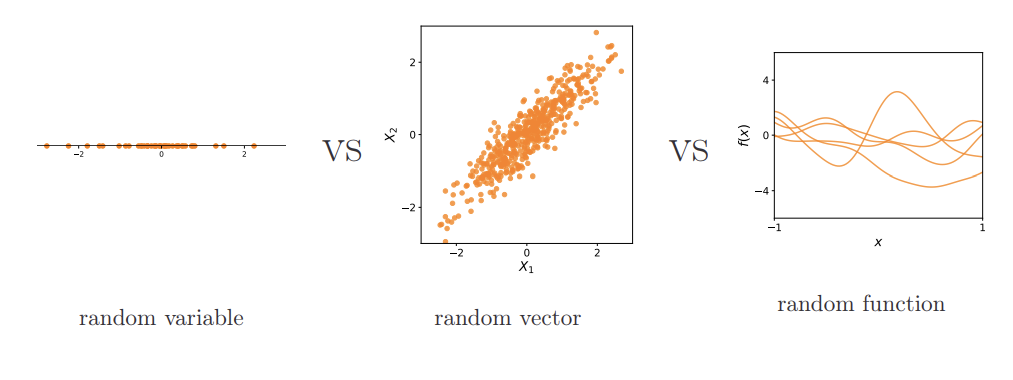
\includegraphics[scale=0.9]{Screenshot 2023-11-28 151344.png}
%     \caption{ \textcolor{red}{Screenshot noch nachbauen} Examples of a random variable, random vector and random process}
%     \label{fig:Screenshot 2023-11-28 151344.png}
% \end{figure}
% 
\begin{figure}[b]
    \centering
    %% Creator: Matplotlib, PGF backend
%%
%% To include the figure in your LaTeX document, write
%%   \input{<filename>.pgf}
%%
%% Make sure the required packages are loaded in your preamble
%%   \usepackage{pgf}
%%
%% Also ensure that all the required font packages are loaded; for instance,
%% the lmodern package is sometimes necessary when using math font.
%%   \usepackage{lmodern}
%%
%% Figures using additional raster images can only be included by \input if
%% they are in the same directory as the main LaTeX file. For loading figures
%% from other directories you can use the `import` package
%%   \usepackage{import}
%%
%% and then include the figures with
%%   \import{<path to file>}{<filename>.pgf}
%%
%% Matplotlib used the following preamble
%%   \def\mathdefault#1{#1}
%%   \everymath=\expandafter{\the\everymath\displaystyle}
%%   \usepackage[T1]{fontenc}
%%   \usepackage{siunitx}
%%   \usepackage{amssymb}
%%   \usepackage{amsmath}
%%   \makeatletter\@ifpackageloaded{underscore}{}{\usepackage[strings]{underscore}}\makeatother
%%
\begingroup%
\makeatletter%
\begin{pgfpicture}%
\pgfpathrectangle{\pgfpointorigin}{\pgfqpoint{5.788510in}{1.788748in}}%
\pgfusepath{use as bounding box, clip}%
\begin{pgfscope}%
\pgfsetbuttcap%
\pgfsetmiterjoin%
\definecolor{currentfill}{rgb}{1.000000,1.000000,1.000000}%
\pgfsetfillcolor{currentfill}%
\pgfsetlinewidth{0.000000pt}%
\definecolor{currentstroke}{rgb}{1.000000,1.000000,1.000000}%
\pgfsetstrokecolor{currentstroke}%
\pgfsetdash{}{0pt}%
\pgfpathmoveto{\pgfqpoint{0.000000in}{0.000000in}}%
\pgfpathlineto{\pgfqpoint{5.788510in}{0.000000in}}%
\pgfpathlineto{\pgfqpoint{5.788510in}{1.788748in}}%
\pgfpathlineto{\pgfqpoint{0.000000in}{1.788748in}}%
\pgfpathlineto{\pgfqpoint{0.000000in}{0.000000in}}%
\pgfpathclose%
\pgfusepath{fill}%
\end{pgfscope}%
\begin{pgfscope}%
\pgfsetbuttcap%
\pgfsetmiterjoin%
\definecolor{currentfill}{rgb}{1.000000,1.000000,1.000000}%
\pgfsetfillcolor{currentfill}%
\pgfsetlinewidth{0.000000pt}%
\definecolor{currentstroke}{rgb}{0.000000,0.000000,0.000000}%
\pgfsetstrokecolor{currentstroke}%
\pgfsetstrokeopacity{0.000000}%
\pgfsetdash{}{0pt}%
\pgfpathmoveto{\pgfqpoint{0.270378in}{0.150000in}}%
\pgfpathlineto{\pgfqpoint{1.759126in}{0.150000in}}%
\pgfpathlineto{\pgfqpoint{1.759126in}{1.638748in}}%
\pgfpathlineto{\pgfqpoint{0.270378in}{1.638748in}}%
\pgfpathlineto{\pgfqpoint{0.270378in}{0.150000in}}%
\pgfpathclose%
\pgfusepath{fill}%
\end{pgfscope}%
\begin{pgfscope}%
\pgfpathrectangle{\pgfqpoint{0.270378in}{0.150000in}}{\pgfqpoint{1.488748in}{1.488748in}}%
\pgfusepath{clip}%
\pgfsetbuttcap%
\pgfsetroundjoin%
\definecolor{currentfill}{rgb}{1.000000,0.745098,0.043137}%
\pgfsetfillcolor{currentfill}%
\pgfsetlinewidth{1.003750pt}%
\definecolor{currentstroke}{rgb}{1.000000,0.745098,0.043137}%
\pgfsetstrokecolor{currentstroke}%
\pgfsetdash{}{0pt}%
\pgfsys@defobject{currentmarker}{\pgfqpoint{-0.004910in}{-0.004910in}}{\pgfqpoint{0.004910in}{0.004910in}}{%
\pgfpathmoveto{\pgfqpoint{0.000000in}{-0.004910in}}%
\pgfpathcurveto{\pgfqpoint{0.001302in}{-0.004910in}}{\pgfqpoint{0.002551in}{-0.004393in}}{\pgfqpoint{0.003472in}{-0.003472in}}%
\pgfpathcurveto{\pgfqpoint{0.004393in}{-0.002551in}}{\pgfqpoint{0.004910in}{-0.001302in}}{\pgfqpoint{0.004910in}{0.000000in}}%
\pgfpathcurveto{\pgfqpoint{0.004910in}{0.001302in}}{\pgfqpoint{0.004393in}{0.002551in}}{\pgfqpoint{0.003472in}{0.003472in}}%
\pgfpathcurveto{\pgfqpoint{0.002551in}{0.004393in}}{\pgfqpoint{0.001302in}{0.004910in}}{\pgfqpoint{0.000000in}{0.004910in}}%
\pgfpathcurveto{\pgfqpoint{-0.001302in}{0.004910in}}{\pgfqpoint{-0.002551in}{0.004393in}}{\pgfqpoint{-0.003472in}{0.003472in}}%
\pgfpathcurveto{\pgfqpoint{-0.004393in}{0.002551in}}{\pgfqpoint{-0.004910in}{0.001302in}}{\pgfqpoint{-0.004910in}{0.000000in}}%
\pgfpathcurveto{\pgfqpoint{-0.004910in}{-0.001302in}}{\pgfqpoint{-0.004393in}{-0.002551in}}{\pgfqpoint{-0.003472in}{-0.003472in}}%
\pgfpathcurveto{\pgfqpoint{-0.002551in}{-0.004393in}}{\pgfqpoint{-0.001302in}{-0.004910in}}{\pgfqpoint{0.000000in}{-0.004910in}}%
\pgfpathlineto{\pgfqpoint{0.000000in}{-0.004910in}}%
\pgfpathclose%
\pgfusepath{stroke,fill}%
}%
\begin{pgfscope}%
\pgfsys@transformshift{0.853307in}{0.894374in}%
\pgfsys@useobject{currentmarker}{}%
\end{pgfscope}%
\begin{pgfscope}%
\pgfsys@transformshift{1.167420in}{0.894374in}%
\pgfsys@useobject{currentmarker}{}%
\end{pgfscope}%
\begin{pgfscope}%
\pgfsys@transformshift{0.912341in}{0.894374in}%
\pgfsys@useobject{currentmarker}{}%
\end{pgfscope}%
\begin{pgfscope}%
\pgfsys@transformshift{0.672276in}{0.894374in}%
\pgfsys@useobject{currentmarker}{}%
\end{pgfscope}%
\begin{pgfscope}%
\pgfsys@transformshift{1.272485in}{0.894374in}%
\pgfsys@useobject{currentmarker}{}%
\end{pgfscope}%
\begin{pgfscope}%
\pgfsys@transformshift{1.312703in}{0.894374in}%
\pgfsys@useobject{currentmarker}{}%
\end{pgfscope}%
\begin{pgfscope}%
\pgfsys@transformshift{1.120275in}{0.894374in}%
\pgfsys@useobject{currentmarker}{}%
\end{pgfscope}%
\begin{pgfscope}%
\pgfsys@transformshift{1.243541in}{0.894374in}%
\pgfsys@useobject{currentmarker}{}%
\end{pgfscope}%
\begin{pgfscope}%
\pgfsys@transformshift{1.163994in}{0.894374in}%
\pgfsys@useobject{currentmarker}{}%
\end{pgfscope}%
\begin{pgfscope}%
\pgfsys@transformshift{1.082993in}{0.894374in}%
\pgfsys@useobject{currentmarker}{}%
\end{pgfscope}%
\begin{pgfscope}%
\pgfsys@transformshift{0.999854in}{0.894374in}%
\pgfsys@useobject{currentmarker}{}%
\end{pgfscope}%
\begin{pgfscope}%
\pgfsys@transformshift{1.262962in}{0.894374in}%
\pgfsys@useobject{currentmarker}{}%
\end{pgfscope}%
\begin{pgfscope}%
\pgfsys@transformshift{1.115710in}{0.894374in}%
\pgfsys@useobject{currentmarker}{}%
\end{pgfscope}%
\begin{pgfscope}%
\pgfsys@transformshift{0.939936in}{0.894374in}%
\pgfsys@useobject{currentmarker}{}%
\end{pgfscope}%
\begin{pgfscope}%
\pgfsys@transformshift{1.264286in}{0.894374in}%
\pgfsys@useobject{currentmarker}{}%
\end{pgfscope}%
\begin{pgfscope}%
\pgfsys@transformshift{1.554554in}{0.894374in}%
\pgfsys@useobject{currentmarker}{}%
\end{pgfscope}%
\begin{pgfscope}%
\pgfsys@transformshift{0.959149in}{0.894374in}%
\pgfsys@useobject{currentmarker}{}%
\end{pgfscope}%
\begin{pgfscope}%
\pgfsys@transformshift{0.511618in}{0.894374in}%
\pgfsys@useobject{currentmarker}{}%
\end{pgfscope}%
\begin{pgfscope}%
\pgfsys@transformshift{0.864650in}{0.894374in}%
\pgfsys@useobject{currentmarker}{}%
\end{pgfscope}%
\begin{pgfscope}%
\pgfsys@transformshift{1.132848in}{0.894374in}%
\pgfsys@useobject{currentmarker}{}%
\end{pgfscope}%
\begin{pgfscope}%
\pgfsys@transformshift{0.719482in}{0.894374in}%
\pgfsys@useobject{currentmarker}{}%
\end{pgfscope}%
\begin{pgfscope}%
\pgfsys@transformshift{1.504550in}{0.894374in}%
\pgfsys@useobject{currentmarker}{}%
\end{pgfscope}%
\begin{pgfscope}%
\pgfsys@transformshift{1.065799in}{0.894374in}%
\pgfsys@useobject{currentmarker}{}%
\end{pgfscope}%
\begin{pgfscope}%
\pgfsys@transformshift{1.362636in}{0.894374in}%
\pgfsys@useobject{currentmarker}{}%
\end{pgfscope}%
\begin{pgfscope}%
\pgfsys@transformshift{0.973301in}{0.894374in}%
\pgfsys@useobject{currentmarker}{}%
\end{pgfscope}%
\begin{pgfscope}%
\pgfsys@transformshift{0.909890in}{0.894374in}%
\pgfsys@useobject{currentmarker}{}%
\end{pgfscope}%
\begin{pgfscope}%
\pgfsys@transformshift{0.963385in}{0.894374in}%
\pgfsys@useobject{currentmarker}{}%
\end{pgfscope}%
\begin{pgfscope}%
\pgfsys@transformshift{1.330969in}{0.894374in}%
\pgfsys@useobject{currentmarker}{}%
\end{pgfscope}%
\begin{pgfscope}%
\pgfsys@transformshift{1.041150in}{0.894374in}%
\pgfsys@useobject{currentmarker}{}%
\end{pgfscope}%
\begin{pgfscope}%
\pgfsys@transformshift{1.153722in}{0.894374in}%
\pgfsys@useobject{currentmarker}{}%
\end{pgfscope}%
\begin{pgfscope}%
\pgfsys@transformshift{0.992481in}{0.894374in}%
\pgfsys@useobject{currentmarker}{}%
\end{pgfscope}%
\begin{pgfscope}%
\pgfsys@transformshift{1.122912in}{0.894374in}%
\pgfsys@useobject{currentmarker}{}%
\end{pgfscope}%
\begin{pgfscope}%
\pgfsys@transformshift{0.338048in}{0.894374in}%
\pgfsys@useobject{currentmarker}{}%
\end{pgfscope}%
\begin{pgfscope}%
\pgfsys@transformshift{0.989402in}{0.894374in}%
\pgfsys@useobject{currentmarker}{}%
\end{pgfscope}%
\begin{pgfscope}%
\pgfsys@transformshift{0.642681in}{0.894374in}%
\pgfsys@useobject{currentmarker}{}%
\end{pgfscope}%
\begin{pgfscope}%
\pgfsys@transformshift{0.938698in}{0.894374in}%
\pgfsys@useobject{currentmarker}{}%
\end{pgfscope}%
\begin{pgfscope}%
\pgfsys@transformshift{1.648253in}{0.894374in}%
\pgfsys@useobject{currentmarker}{}%
\end{pgfscope}%
\begin{pgfscope}%
\pgfsys@transformshift{0.931664in}{0.894374in}%
\pgfsys@useobject{currentmarker}{}%
\end{pgfscope}%
\begin{pgfscope}%
\pgfsys@transformshift{1.105766in}{0.894374in}%
\pgfsys@useobject{currentmarker}{}%
\end{pgfscope}%
\begin{pgfscope}%
\pgfsys@transformshift{1.691455in}{0.894374in}%
\pgfsys@useobject{currentmarker}{}%
\end{pgfscope}%
\begin{pgfscope}%
\pgfsys@transformshift{1.490737in}{0.894374in}%
\pgfsys@useobject{currentmarker}{}%
\end{pgfscope}%
\begin{pgfscope}%
\pgfsys@transformshift{0.574491in}{0.894374in}%
\pgfsys@useobject{currentmarker}{}%
\end{pgfscope}%
\begin{pgfscope}%
\pgfsys@transformshift{1.437226in}{0.894374in}%
\pgfsys@useobject{currentmarker}{}%
\end{pgfscope}%
\begin{pgfscope}%
\pgfsys@transformshift{1.115643in}{0.894374in}%
\pgfsys@useobject{currentmarker}{}%
\end{pgfscope}%
\begin{pgfscope}%
\pgfsys@transformshift{1.047076in}{0.894374in}%
\pgfsys@useobject{currentmarker}{}%
\end{pgfscope}%
\begin{pgfscope}%
\pgfsys@transformshift{1.263964in}{0.894374in}%
\pgfsys@useobject{currentmarker}{}%
\end{pgfscope}%
\begin{pgfscope}%
\pgfsys@transformshift{1.019037in}{0.894374in}%
\pgfsys@useobject{currentmarker}{}%
\end{pgfscope}%
\begin{pgfscope}%
\pgfsys@transformshift{1.204106in}{0.894374in}%
\pgfsys@useobject{currentmarker}{}%
\end{pgfscope}%
\begin{pgfscope}%
\pgfsys@transformshift{1.103160in}{0.894374in}%
\pgfsys@useobject{currentmarker}{}%
\end{pgfscope}%
\begin{pgfscope}%
\pgfsys@transformshift{1.316196in}{0.894374in}%
\pgfsys@useobject{currentmarker}{}%
\end{pgfscope}%
\end{pgfscope}%
\begin{pgfscope}%
\pgfsetbuttcap%
\pgfsetmiterjoin%
\definecolor{currentfill}{rgb}{1.000000,1.000000,1.000000}%
\pgfsetfillcolor{currentfill}%
\pgfsetlinewidth{0.000000pt}%
\definecolor{currentstroke}{rgb}{0.000000,0.000000,0.000000}%
\pgfsetstrokecolor{currentstroke}%
\pgfsetstrokeopacity{0.000000}%
\pgfsetdash{}{0pt}%
\pgfpathmoveto{\pgfqpoint{2.149881in}{0.150000in}}%
\pgfpathlineto{\pgfqpoint{3.638629in}{0.150000in}}%
\pgfpathlineto{\pgfqpoint{3.638629in}{1.638748in}}%
\pgfpathlineto{\pgfqpoint{2.149881in}{1.638748in}}%
\pgfpathlineto{\pgfqpoint{2.149881in}{0.150000in}}%
\pgfpathclose%
\pgfusepath{fill}%
\end{pgfscope}%
\begin{pgfscope}%
\pgfpathrectangle{\pgfqpoint{2.149881in}{0.150000in}}{\pgfqpoint{1.488748in}{1.488748in}}%
\pgfusepath{clip}%
\pgfsetbuttcap%
\pgfsetroundjoin%
\definecolor{currentfill}{rgb}{1.000000,0.745098,0.043137}%
\pgfsetfillcolor{currentfill}%
\pgfsetlinewidth{1.003750pt}%
\definecolor{currentstroke}{rgb}{1.000000,0.745098,0.043137}%
\pgfsetstrokecolor{currentstroke}%
\pgfsetdash{}{0pt}%
\pgfsys@defobject{currentmarker}{\pgfqpoint{-0.004910in}{-0.004910in}}{\pgfqpoint{0.004910in}{0.004910in}}{%
\pgfpathmoveto{\pgfqpoint{0.000000in}{-0.004910in}}%
\pgfpathcurveto{\pgfqpoint{0.001302in}{-0.004910in}}{\pgfqpoint{0.002551in}{-0.004393in}}{\pgfqpoint{0.003472in}{-0.003472in}}%
\pgfpathcurveto{\pgfqpoint{0.004393in}{-0.002551in}}{\pgfqpoint{0.004910in}{-0.001302in}}{\pgfqpoint{0.004910in}{0.000000in}}%
\pgfpathcurveto{\pgfqpoint{0.004910in}{0.001302in}}{\pgfqpoint{0.004393in}{0.002551in}}{\pgfqpoint{0.003472in}{0.003472in}}%
\pgfpathcurveto{\pgfqpoint{0.002551in}{0.004393in}}{\pgfqpoint{0.001302in}{0.004910in}}{\pgfqpoint{0.000000in}{0.004910in}}%
\pgfpathcurveto{\pgfqpoint{-0.001302in}{0.004910in}}{\pgfqpoint{-0.002551in}{0.004393in}}{\pgfqpoint{-0.003472in}{0.003472in}}%
\pgfpathcurveto{\pgfqpoint{-0.004393in}{0.002551in}}{\pgfqpoint{-0.004910in}{0.001302in}}{\pgfqpoint{-0.004910in}{0.000000in}}%
\pgfpathcurveto{\pgfqpoint{-0.004910in}{-0.001302in}}{\pgfqpoint{-0.004393in}{-0.002551in}}{\pgfqpoint{-0.003472in}{-0.003472in}}%
\pgfpathcurveto{\pgfqpoint{-0.002551in}{-0.004393in}}{\pgfqpoint{-0.001302in}{-0.004910in}}{\pgfqpoint{0.000000in}{-0.004910in}}%
\pgfpathlineto{\pgfqpoint{0.000000in}{-0.004910in}}%
\pgfpathclose%
\pgfusepath{stroke,fill}%
}%
\begin{pgfscope}%
\pgfsys@transformshift{3.292183in}{0.820815in}%
\pgfsys@useobject{currentmarker}{}%
\end{pgfscope}%
\begin{pgfscope}%
\pgfsys@transformshift{2.766297in}{1.074182in}%
\pgfsys@useobject{currentmarker}{}%
\end{pgfscope}%
\begin{pgfscope}%
\pgfsys@transformshift{3.016164in}{0.868433in}%
\pgfsys@useobject{currentmarker}{}%
\end{pgfscope}%
\begin{pgfscope}%
\pgfsys@transformshift{3.393389in}{0.674793in}%
\pgfsys@useobject{currentmarker}{}%
\end{pgfscope}%
\begin{pgfscope}%
\pgfsys@transformshift{2.599394in}{1.158929in}%
\pgfsys@useobject{currentmarker}{}%
\end{pgfscope}%
\begin{pgfscope}%
\pgfsys@transformshift{2.698329in}{1.191369in}%
\pgfsys@useobject{currentmarker}{}%
\end{pgfscope}%
\begin{pgfscope}%
\pgfsys@transformshift{3.101029in}{1.036154in}%
\pgfsys@useobject{currentmarker}{}%
\end{pgfscope}%
\begin{pgfscope}%
\pgfsys@transformshift{2.814634in}{1.135583in}%
\pgfsys@useobject{currentmarker}{}%
\end{pgfscope}%
\begin{pgfscope}%
\pgfsys@transformshift{2.970497in}{1.071419in}%
\pgfsys@useobject{currentmarker}{}%
\end{pgfscope}%
\begin{pgfscope}%
\pgfsys@transformshift{3.199209in}{1.006082in}%
\pgfsys@useobject{currentmarker}{}%
\end{pgfscope}%
\begin{pgfscope}%
\pgfsys@transformshift{2.902039in}{0.939021in}%
\pgfsys@useobject{currentmarker}{}%
\end{pgfscope}%
\begin{pgfscope}%
\pgfsys@transformshift{2.812665in}{1.151247in}%
\pgfsys@useobject{currentmarker}{}%
\end{pgfscope}%
\begin{pgfscope}%
\pgfsys@transformshift{3.170300in}{1.032472in}%
\pgfsys@useobject{currentmarker}{}%
\end{pgfscope}%
\begin{pgfscope}%
\pgfsys@transformshift{3.124205in}{0.890691in}%
\pgfsys@useobject{currentmarker}{}%
\end{pgfscope}%
\begin{pgfscope}%
\pgfsys@transformshift{2.844550in}{1.152315in}%
\pgfsys@useobject{currentmarker}{}%
\end{pgfscope}%
\begin{pgfscope}%
\pgfsys@transformshift{2.877353in}{1.386449in}%
\pgfsys@useobject{currentmarker}{}%
\end{pgfscope}%
\begin{pgfscope}%
\pgfsys@transformshift{3.237843in}{0.906188in}%
\pgfsys@useobject{currentmarker}{}%
\end{pgfscope}%
\begin{pgfscope}%
\pgfsys@transformshift{3.271953in}{0.545204in}%
\pgfsys@useobject{currentmarker}{}%
\end{pgfscope}%
\begin{pgfscope}%
\pgfsys@transformshift{3.130046in}{0.829964in}%
\pgfsys@useobject{currentmarker}{}%
\end{pgfscope}%
\begin{pgfscope}%
\pgfsys@transformshift{2.732968in}{1.046296in}%
\pgfsys@useobject{currentmarker}{}%
\end{pgfscope}%
\begin{pgfscope}%
\pgfsys@transformshift{3.292562in}{0.712870in}%
\pgfsys@useobject{currentmarker}{}%
\end{pgfscope}%
\begin{pgfscope}%
\pgfsys@transformshift{2.482950in}{1.346115in}%
\pgfsys@useobject{currentmarker}{}%
\end{pgfscope}%
\begin{pgfscope}%
\pgfsys@transformshift{2.826043in}{0.992214in}%
\pgfsys@useobject{currentmarker}{}%
\end{pgfscope}%
\begin{pgfscope}%
\pgfsys@transformshift{2.777339in}{1.231646in}%
\pgfsys@useobject{currentmarker}{}%
\end{pgfscope}%
\begin{pgfscope}%
\pgfsys@transformshift{3.118964in}{0.917603in}%
\pgfsys@useobject{currentmarker}{}%
\end{pgfscope}%
\begin{pgfscope}%
\pgfsys@transformshift{3.099844in}{0.866455in}%
\pgfsys@useobject{currentmarker}{}%
\end{pgfscope}%
\begin{pgfscope}%
\pgfsys@transformshift{2.886776in}{0.909605in}%
\pgfsys@useobject{currentmarker}{}%
\end{pgfscope}%
\begin{pgfscope}%
\pgfsys@transformshift{2.528690in}{1.206103in}%
\pgfsys@useobject{currentmarker}{}%
\end{pgfscope}%
\begin{pgfscope}%
\pgfsys@transformshift{2.921993in}{0.972331in}%
\pgfsys@useobject{currentmarker}{}%
\end{pgfscope}%
\begin{pgfscope}%
\pgfsys@transformshift{2.820265in}{1.063134in}%
\pgfsys@useobject{currentmarker}{}%
\end{pgfscope}%
\begin{pgfscope}%
\pgfsys@transformshift{2.819231in}{0.933074in}%
\pgfsys@useobject{currentmarker}{}%
\end{pgfscope}%
\begin{pgfscope}%
\pgfsys@transformshift{2.909380in}{1.038282in}%
\pgfsys@useobject{currentmarker}{}%
\end{pgfscope}%
\begin{pgfscope}%
\pgfsys@transformshift{3.343094in}{0.405201in}%
\pgfsys@useobject{currentmarker}{}%
\end{pgfscope}%
\begin{pgfscope}%
\pgfsys@transformshift{3.210079in}{0.930591in}%
\pgfsys@useobject{currentmarker}{}%
\end{pgfscope}%
\begin{pgfscope}%
\pgfsys@transformshift{3.290044in}{0.650921in}%
\pgfsys@useobject{currentmarker}{}%
\end{pgfscope}%
\begin{pgfscope}%
\pgfsys@transformshift{2.956844in}{0.889692in}%
\pgfsys@useobject{currentmarker}{}%
\end{pgfscope}%
\begin{pgfscope}%
\pgfsys@transformshift{2.623165in}{1.462028in}%
\pgfsys@useobject{currentmarker}{}%
\end{pgfscope}%
\begin{pgfscope}%
\pgfsys@transformshift{2.891824in}{0.884019in}%
\pgfsys@useobject{currentmarker}{}%
\end{pgfscope}%
\begin{pgfscope}%
\pgfsys@transformshift{3.030991in}{1.024452in}%
\pgfsys@useobject{currentmarker}{}%
\end{pgfscope}%
\begin{pgfscope}%
\pgfsys@transformshift{2.900213in}{1.496876in}%
\pgfsys@useobject{currentmarker}{}%
\end{pgfscope}%
\begin{pgfscope}%
\pgfsys@transformshift{2.636254in}{1.334974in}%
\pgfsys@useobject{currentmarker}{}%
\end{pgfscope}%
\begin{pgfscope}%
\pgfsys@transformshift{3.274368in}{0.595918in}%
\pgfsys@useobject{currentmarker}{}%
\end{pgfscope}%
\begin{pgfscope}%
\pgfsys@transformshift{2.716049in}{1.291811in}%
\pgfsys@useobject{currentmarker}{}%
\end{pgfscope}%
\begin{pgfscope}%
\pgfsys@transformshift{2.888498in}{1.032418in}%
\pgfsys@useobject{currentmarker}{}%
\end{pgfscope}%
\begin{pgfscope}%
\pgfsys@transformshift{2.963671in}{0.977112in}%
\pgfsys@useobject{currentmarker}{}%
\end{pgfscope}%
\begin{pgfscope}%
\pgfsys@transformshift{2.966203in}{1.152056in}%
\pgfsys@useobject{currentmarker}{}%
\end{pgfscope}%
\begin{pgfscope}%
\pgfsys@transformshift{3.020282in}{0.954495in}%
\pgfsys@useobject{currentmarker}{}%
\end{pgfscope}%
\begin{pgfscope}%
\pgfsys@transformshift{3.020831in}{1.103774in}%
\pgfsys@useobject{currentmarker}{}%
\end{pgfscope}%
\begin{pgfscope}%
\pgfsys@transformshift{2.752522in}{1.022349in}%
\pgfsys@useobject{currentmarker}{}%
\end{pgfscope}%
\begin{pgfscope}%
\pgfsys@transformshift{2.841155in}{1.194187in}%
\pgfsys@useobject{currentmarker}{}%
\end{pgfscope}%
\begin{pgfscope}%
\pgfsys@transformshift{3.136736in}{0.805025in}%
\pgfsys@useobject{currentmarker}{}%
\end{pgfscope}%
\begin{pgfscope}%
\pgfsys@transformshift{2.918830in}{1.384175in}%
\pgfsys@useobject{currentmarker}{}%
\end{pgfscope}%
\begin{pgfscope}%
\pgfsys@transformshift{3.158122in}{0.516969in}%
\pgfsys@useobject{currentmarker}{}%
\end{pgfscope}%
\begin{pgfscope}%
\pgfsys@transformshift{3.150810in}{0.476784in}%
\pgfsys@useobject{currentmarker}{}%
\end{pgfscope}%
\begin{pgfscope}%
\pgfsys@transformshift{2.918541in}{0.795489in}%
\pgfsys@useobject{currentmarker}{}%
\end{pgfscope}%
\begin{pgfscope}%
\pgfsys@transformshift{2.437682in}{1.336634in}%
\pgfsys@useobject{currentmarker}{}%
\end{pgfscope}%
\begin{pgfscope}%
\pgfsys@transformshift{3.003925in}{1.039181in}%
\pgfsys@useobject{currentmarker}{}%
\end{pgfscope}%
\begin{pgfscope}%
\pgfsys@transformshift{3.398152in}{0.758225in}%
\pgfsys@useobject{currentmarker}{}%
\end{pgfscope}%
\begin{pgfscope}%
\pgfsys@transformshift{3.485491in}{0.460491in}%
\pgfsys@useobject{currentmarker}{}%
\end{pgfscope}%
\begin{pgfscope}%
\pgfsys@transformshift{2.879639in}{1.169808in}%
\pgfsys@useobject{currentmarker}{}%
\end{pgfscope}%
\begin{pgfscope}%
\pgfsys@transformshift{2.978119in}{0.986668in}%
\pgfsys@useobject{currentmarker}{}%
\end{pgfscope}%
\begin{pgfscope}%
\pgfsys@transformshift{2.438617in}{1.496893in}%
\pgfsys@useobject{currentmarker}{}%
\end{pgfscope}%
\begin{pgfscope}%
\pgfsys@transformshift{3.001535in}{1.218313in}%
\pgfsys@useobject{currentmarker}{}%
\end{pgfscope}%
\begin{pgfscope}%
\pgfsys@transformshift{2.639058in}{1.084074in}%
\pgfsys@useobject{currentmarker}{}%
\end{pgfscope}%
\begin{pgfscope}%
\pgfsys@transformshift{2.979408in}{1.121190in}%
\pgfsys@useobject{currentmarker}{}%
\end{pgfscope}%
\begin{pgfscope}%
\pgfsys@transformshift{3.176590in}{0.751090in}%
\pgfsys@useobject{currentmarker}{}%
\end{pgfscope}%
\begin{pgfscope}%
\pgfsys@transformshift{2.981850in}{1.173095in}%
\pgfsys@useobject{currentmarker}{}%
\end{pgfscope}%
\begin{pgfscope}%
\pgfsys@transformshift{3.202145in}{0.867681in}%
\pgfsys@useobject{currentmarker}{}%
\end{pgfscope}%
\begin{pgfscope}%
\pgfsys@transformshift{2.946546in}{1.141761in}%
\pgfsys@useobject{currentmarker}{}%
\end{pgfscope}%
\begin{pgfscope}%
\pgfsys@transformshift{2.948710in}{1.212875in}%
\pgfsys@useobject{currentmarker}{}%
\end{pgfscope}%
\begin{pgfscope}%
\pgfsys@transformshift{3.050329in}{0.771247in}%
\pgfsys@useobject{currentmarker}{}%
\end{pgfscope}%
\begin{pgfscope}%
\pgfsys@transformshift{3.570959in}{0.591994in}%
\pgfsys@useobject{currentmarker}{}%
\end{pgfscope}%
\begin{pgfscope}%
\pgfsys@transformshift{3.237305in}{0.991549in}%
\pgfsys@useobject{currentmarker}{}%
\end{pgfscope}%
\begin{pgfscope}%
\pgfsys@transformshift{2.670376in}{0.961162in}%
\pgfsys@useobject{currentmarker}{}%
\end{pgfscope}%
\begin{pgfscope}%
\pgfsys@transformshift{3.008122in}{1.170816in}%
\pgfsys@useobject{currentmarker}{}%
\end{pgfscope}%
\begin{pgfscope}%
\pgfsys@transformshift{3.128020in}{0.883333in}%
\pgfsys@useobject{currentmarker}{}%
\end{pgfscope}%
\begin{pgfscope}%
\pgfsys@transformshift{3.296901in}{1.044916in}%
\pgfsys@useobject{currentmarker}{}%
\end{pgfscope}%
\begin{pgfscope}%
\pgfsys@transformshift{3.022358in}{1.041996in}%
\pgfsys@useobject{currentmarker}{}%
\end{pgfscope}%
\begin{pgfscope}%
\pgfsys@transformshift{2.642266in}{1.096272in}%
\pgfsys@useobject{currentmarker}{}%
\end{pgfscope}%
\begin{pgfscope}%
\pgfsys@transformshift{2.910023in}{0.842787in}%
\pgfsys@useobject{currentmarker}{}%
\end{pgfscope}%
\begin{pgfscope}%
\pgfsys@transformshift{2.830219in}{1.434204in}%
\pgfsys@useobject{currentmarker}{}%
\end{pgfscope}%
\begin{pgfscope}%
\pgfsys@transformshift{3.055853in}{1.015857in}%
\pgfsys@useobject{currentmarker}{}%
\end{pgfscope}%
\begin{pgfscope}%
\pgfsys@transformshift{3.300423in}{0.422005in}%
\pgfsys@useobject{currentmarker}{}%
\end{pgfscope}%
\begin{pgfscope}%
\pgfsys@transformshift{3.156292in}{0.701305in}%
\pgfsys@useobject{currentmarker}{}%
\end{pgfscope}%
\begin{pgfscope}%
\pgfsys@transformshift{3.120431in}{1.027413in}%
\pgfsys@useobject{currentmarker}{}%
\end{pgfscope}%
\begin{pgfscope}%
\pgfsys@transformshift{2.826281in}{0.897525in}%
\pgfsys@useobject{currentmarker}{}%
\end{pgfscope}%
\begin{pgfscope}%
\pgfsys@transformshift{3.069099in}{1.224011in}%
\pgfsys@useobject{currentmarker}{}%
\end{pgfscope}%
\begin{pgfscope}%
\pgfsys@transformshift{2.856950in}{0.916958in}%
\pgfsys@useobject{currentmarker}{}%
\end{pgfscope}%
\begin{pgfscope}%
\pgfsys@transformshift{3.005903in}{0.783774in}%
\pgfsys@useobject{currentmarker}{}%
\end{pgfscope}%
\begin{pgfscope}%
\pgfsys@transformshift{2.590458in}{1.236556in}%
\pgfsys@useobject{currentmarker}{}%
\end{pgfscope}%
\begin{pgfscope}%
\pgfsys@transformshift{3.025202in}{0.870818in}%
\pgfsys@useobject{currentmarker}{}%
\end{pgfscope}%
\begin{pgfscope}%
\pgfsys@transformshift{2.861535in}{1.399076in}%
\pgfsys@useobject{currentmarker}{}%
\end{pgfscope}%
\begin{pgfscope}%
\pgfsys@transformshift{2.865465in}{1.046632in}%
\pgfsys@useobject{currentmarker}{}%
\end{pgfscope}%
\begin{pgfscope}%
\pgfsys@transformshift{3.291175in}{0.886398in}%
\pgfsys@useobject{currentmarker}{}%
\end{pgfscope}%
\begin{pgfscope}%
\pgfsys@transformshift{2.924942in}{0.973597in}%
\pgfsys@useobject{currentmarker}{}%
\end{pgfscope}%
\begin{pgfscope}%
\pgfsys@transformshift{3.158338in}{0.919368in}%
\pgfsys@useobject{currentmarker}{}%
\end{pgfscope}%
\begin{pgfscope}%
\pgfsys@transformshift{2.943787in}{0.803155in}%
\pgfsys@useobject{currentmarker}{}%
\end{pgfscope}%
\begin{pgfscope}%
\pgfsys@transformshift{2.821640in}{0.883277in}%
\pgfsys@useobject{currentmarker}{}%
\end{pgfscope}%
\begin{pgfscope}%
\pgfsys@transformshift{3.156815in}{0.656475in}%
\pgfsys@useobject{currentmarker}{}%
\end{pgfscope}%
\begin{pgfscope}%
\pgfsys@transformshift{2.999820in}{0.789821in}%
\pgfsys@useobject{currentmarker}{}%
\end{pgfscope}%
\begin{pgfscope}%
\pgfsys@transformshift{3.173224in}{1.095105in}%
\pgfsys@useobject{currentmarker}{}%
\end{pgfscope}%
\begin{pgfscope}%
\pgfsys@transformshift{3.070342in}{0.938471in}%
\pgfsys@useobject{currentmarker}{}%
\end{pgfscope}%
\begin{pgfscope}%
\pgfsys@transformshift{3.104600in}{0.574130in}%
\pgfsys@useobject{currentmarker}{}%
\end{pgfscope}%
\begin{pgfscope}%
\pgfsys@transformshift{2.937220in}{1.157010in}%
\pgfsys@useobject{currentmarker}{}%
\end{pgfscope}%
\begin{pgfscope}%
\pgfsys@transformshift{2.873278in}{0.765679in}%
\pgfsys@useobject{currentmarker}{}%
\end{pgfscope}%
\begin{pgfscope}%
\pgfsys@transformshift{2.984608in}{1.088477in}%
\pgfsys@useobject{currentmarker}{}%
\end{pgfscope}%
\begin{pgfscope}%
\pgfsys@transformshift{3.121201in}{0.559318in}%
\pgfsys@useobject{currentmarker}{}%
\end{pgfscope}%
\begin{pgfscope}%
\pgfsys@transformshift{2.898886in}{1.539487in}%
\pgfsys@useobject{currentmarker}{}%
\end{pgfscope}%
\begin{pgfscope}%
\pgfsys@transformshift{3.557581in}{0.830091in}%
\pgfsys@useobject{currentmarker}{}%
\end{pgfscope}%
\begin{pgfscope}%
\pgfsys@transformshift{2.854913in}{1.141458in}%
\pgfsys@useobject{currentmarker}{}%
\end{pgfscope}%
\begin{pgfscope}%
\pgfsys@transformshift{2.641077in}{1.058083in}%
\pgfsys@useobject{currentmarker}{}%
\end{pgfscope}%
\begin{pgfscope}%
\pgfsys@transformshift{3.052658in}{0.849811in}%
\pgfsys@useobject{currentmarker}{}%
\end{pgfscope}%
\begin{pgfscope}%
\pgfsys@transformshift{2.712948in}{1.135818in}%
\pgfsys@useobject{currentmarker}{}%
\end{pgfscope}%
\begin{pgfscope}%
\pgfsys@transformshift{3.025048in}{0.957884in}%
\pgfsys@useobject{currentmarker}{}%
\end{pgfscope}%
\begin{pgfscope}%
\pgfsys@transformshift{3.232194in}{0.644656in}%
\pgfsys@useobject{currentmarker}{}%
\end{pgfscope}%
\begin{pgfscope}%
\pgfsys@transformshift{3.174711in}{0.854507in}%
\pgfsys@useobject{currentmarker}{}%
\end{pgfscope}%
\begin{pgfscope}%
\pgfsys@transformshift{2.863597in}{0.880833in}%
\pgfsys@useobject{currentmarker}{}%
\end{pgfscope}%
\begin{pgfscope}%
\pgfsys@transformshift{2.810612in}{1.031985in}%
\pgfsys@useobject{currentmarker}{}%
\end{pgfscope}%
\begin{pgfscope}%
\pgfsys@transformshift{2.920240in}{1.125349in}%
\pgfsys@useobject{currentmarker}{}%
\end{pgfscope}%
\begin{pgfscope}%
\pgfsys@transformshift{3.129141in}{0.999864in}%
\pgfsys@useobject{currentmarker}{}%
\end{pgfscope}%
\begin{pgfscope}%
\pgfsys@transformshift{3.094856in}{0.893336in}%
\pgfsys@useobject{currentmarker}{}%
\end{pgfscope}%
\begin{pgfscope}%
\pgfsys@transformshift{3.004932in}{1.138651in}%
\pgfsys@useobject{currentmarker}{}%
\end{pgfscope}%
\begin{pgfscope}%
\pgfsys@transformshift{3.244151in}{0.398879in}%
\pgfsys@useobject{currentmarker}{}%
\end{pgfscope}%
\begin{pgfscope}%
\pgfsys@transformshift{2.876036in}{1.001852in}%
\pgfsys@useobject{currentmarker}{}%
\end{pgfscope}%
\begin{pgfscope}%
\pgfsys@transformshift{2.912317in}{0.933664in}%
\pgfsys@useobject{currentmarker}{}%
\end{pgfscope}%
\begin{pgfscope}%
\pgfsys@transformshift{2.942975in}{0.989561in}%
\pgfsys@useobject{currentmarker}{}%
\end{pgfscope}%
\begin{pgfscope}%
\pgfsys@transformshift{2.920816in}{1.406732in}%
\pgfsys@useobject{currentmarker}{}%
\end{pgfscope}%
\begin{pgfscope}%
\pgfsys@transformshift{3.016320in}{0.980359in}%
\pgfsys@useobject{currentmarker}{}%
\end{pgfscope}%
\begin{pgfscope}%
\pgfsys@transformshift{2.689784in}{1.199247in}%
\pgfsys@useobject{currentmarker}{}%
\end{pgfscope}%
\begin{pgfscope}%
\pgfsys@transformshift{3.102604in}{0.959324in}%
\pgfsys@useobject{currentmarker}{}%
\end{pgfscope}%
\begin{pgfscope}%
\pgfsys@transformshift{3.093733in}{0.873362in}%
\pgfsys@useobject{currentmarker}{}%
\end{pgfscope}%
\begin{pgfscope}%
\pgfsys@transformshift{3.094146in}{0.940765in}%
\pgfsys@useobject{currentmarker}{}%
\end{pgfscope}%
\begin{pgfscope}%
\pgfsys@transformshift{2.918473in}{1.085305in}%
\pgfsys@useobject{currentmarker}{}%
\end{pgfscope}%
\begin{pgfscope}%
\pgfsys@transformshift{2.963545in}{1.000984in}%
\pgfsys@useobject{currentmarker}{}%
\end{pgfscope}%
\begin{pgfscope}%
\pgfsys@transformshift{3.202927in}{0.660807in}%
\pgfsys@useobject{currentmarker}{}%
\end{pgfscope}%
\begin{pgfscope}%
\pgfsys@transformshift{3.214552in}{0.782652in}%
\pgfsys@useobject{currentmarker}{}%
\end{pgfscope}%
\begin{pgfscope}%
\pgfsys@transformshift{2.852498in}{1.165537in}%
\pgfsys@useobject{currentmarker}{}%
\end{pgfscope}%
\begin{pgfscope}%
\pgfsys@transformshift{2.979304in}{0.978036in}%
\pgfsys@useobject{currentmarker}{}%
\end{pgfscope}%
\begin{pgfscope}%
\pgfsys@transformshift{3.075529in}{1.045012in}%
\pgfsys@useobject{currentmarker}{}%
\end{pgfscope}%
\begin{pgfscope}%
\pgfsys@transformshift{2.683744in}{1.260661in}%
\pgfsys@useobject{currentmarker}{}%
\end{pgfscope}%
\begin{pgfscope}%
\pgfsys@transformshift{2.914105in}{0.960025in}%
\pgfsys@useobject{currentmarker}{}%
\end{pgfscope}%
\begin{pgfscope}%
\pgfsys@transformshift{2.739068in}{1.388912in}%
\pgfsys@useobject{currentmarker}{}%
\end{pgfscope}%
\begin{pgfscope}%
\pgfsys@transformshift{2.829750in}{1.215005in}%
\pgfsys@useobject{currentmarker}{}%
\end{pgfscope}%
\begin{pgfscope}%
\pgfsys@transformshift{2.959678in}{0.909226in}%
\pgfsys@useobject{currentmarker}{}%
\end{pgfscope}%
\begin{pgfscope}%
\pgfsys@transformshift{3.449945in}{0.564964in}%
\pgfsys@useobject{currentmarker}{}%
\end{pgfscope}%
\begin{pgfscope}%
\pgfsys@transformshift{2.869755in}{0.996159in}%
\pgfsys@useobject{currentmarker}{}%
\end{pgfscope}%
\begin{pgfscope}%
\pgfsys@transformshift{3.121885in}{1.167109in}%
\pgfsys@useobject{currentmarker}{}%
\end{pgfscope}%
\begin{pgfscope}%
\pgfsys@transformshift{2.632255in}{1.262669in}%
\pgfsys@useobject{currentmarker}{}%
\end{pgfscope}%
\begin{pgfscope}%
\pgfsys@transformshift{3.096825in}{0.679577in}%
\pgfsys@useobject{currentmarker}{}%
\end{pgfscope}%
\begin{pgfscope}%
\pgfsys@transformshift{2.843016in}{1.285787in}%
\pgfsys@useobject{currentmarker}{}%
\end{pgfscope}%
\begin{pgfscope}%
\pgfsys@transformshift{3.123207in}{0.711252in}%
\pgfsys@useobject{currentmarker}{}%
\end{pgfscope}%
\begin{pgfscope}%
\pgfsys@transformshift{2.815359in}{1.458044in}%
\pgfsys@useobject{currentmarker}{}%
\end{pgfscope}%
\begin{pgfscope}%
\pgfsys@transformshift{3.316818in}{0.898133in}%
\pgfsys@useobject{currentmarker}{}%
\end{pgfscope}%
\begin{pgfscope}%
\pgfsys@transformshift{3.065039in}{0.812145in}%
\pgfsys@useobject{currentmarker}{}%
\end{pgfscope}%
\begin{pgfscope}%
\pgfsys@transformshift{2.791945in}{1.398995in}%
\pgfsys@useobject{currentmarker}{}%
\end{pgfscope}%
\begin{pgfscope}%
\pgfsys@transformshift{3.055654in}{1.030715in}%
\pgfsys@useobject{currentmarker}{}%
\end{pgfscope}%
\begin{pgfscope}%
\pgfsys@transformshift{2.661285in}{1.213917in}%
\pgfsys@useobject{currentmarker}{}%
\end{pgfscope}%
\begin{pgfscope}%
\pgfsys@transformshift{3.013580in}{0.845917in}%
\pgfsys@useobject{currentmarker}{}%
\end{pgfscope}%
\begin{pgfscope}%
\pgfsys@transformshift{2.699226in}{1.170671in}%
\pgfsys@useobject{currentmarker}{}%
\end{pgfscope}%
\begin{pgfscope}%
\pgfsys@transformshift{3.047210in}{0.945306in}%
\pgfsys@useobject{currentmarker}{}%
\end{pgfscope}%
\begin{pgfscope}%
\pgfsys@transformshift{2.626336in}{1.088588in}%
\pgfsys@useobject{currentmarker}{}%
\end{pgfscope}%
\begin{pgfscope}%
\pgfsys@transformshift{3.058079in}{0.664534in}%
\pgfsys@useobject{currentmarker}{}%
\end{pgfscope}%
\begin{pgfscope}%
\pgfsys@transformshift{3.024086in}{1.037259in}%
\pgfsys@useobject{currentmarker}{}%
\end{pgfscope}%
\begin{pgfscope}%
\pgfsys@transformshift{2.791240in}{1.215283in}%
\pgfsys@useobject{currentmarker}{}%
\end{pgfscope}%
\begin{pgfscope}%
\pgfsys@transformshift{2.953239in}{1.288366in}%
\pgfsys@useobject{currentmarker}{}%
\end{pgfscope}%
\begin{pgfscope}%
\pgfsys@transformshift{2.646429in}{0.942844in}%
\pgfsys@useobject{currentmarker}{}%
\end{pgfscope}%
\begin{pgfscope}%
\pgfsys@transformshift{2.983775in}{0.997191in}%
\pgfsys@useobject{currentmarker}{}%
\end{pgfscope}%
\begin{pgfscope}%
\pgfsys@transformshift{3.004487in}{0.894879in}%
\pgfsys@useobject{currentmarker}{}%
\end{pgfscope}%
\begin{pgfscope}%
\pgfsys@transformshift{3.281238in}{0.869980in}%
\pgfsys@useobject{currentmarker}{}%
\end{pgfscope}%
\begin{pgfscope}%
\pgfsys@transformshift{2.871144in}{1.324557in}%
\pgfsys@useobject{currentmarker}{}%
\end{pgfscope}%
\begin{pgfscope}%
\pgfsys@transformshift{2.982777in}{0.842417in}%
\pgfsys@useobject{currentmarker}{}%
\end{pgfscope}%
\begin{pgfscope}%
\pgfsys@transformshift{3.374172in}{0.565067in}%
\pgfsys@useobject{currentmarker}{}%
\end{pgfscope}%
\begin{pgfscope}%
\pgfsys@transformshift{3.051627in}{1.214210in}%
\pgfsys@useobject{currentmarker}{}%
\end{pgfscope}%
\begin{pgfscope}%
\pgfsys@transformshift{2.677908in}{1.374981in}%
\pgfsys@useobject{currentmarker}{}%
\end{pgfscope}%
\begin{pgfscope}%
\pgfsys@transformshift{3.187682in}{0.662551in}%
\pgfsys@useobject{currentmarker}{}%
\end{pgfscope}%
\begin{pgfscope}%
\pgfsys@transformshift{3.286411in}{0.774165in}%
\pgfsys@useobject{currentmarker}{}%
\end{pgfscope}%
\begin{pgfscope}%
\pgfsys@transformshift{2.862629in}{0.890600in}%
\pgfsys@useobject{currentmarker}{}%
\end{pgfscope}%
\begin{pgfscope}%
\pgfsys@transformshift{3.041578in}{0.947571in}%
\pgfsys@useobject{currentmarker}{}%
\end{pgfscope}%
\begin{pgfscope}%
\pgfsys@transformshift{2.401452in}{1.471491in}%
\pgfsys@useobject{currentmarker}{}%
\end{pgfscope}%
\begin{pgfscope}%
\pgfsys@transformshift{3.174531in}{1.298846in}%
\pgfsys@useobject{currentmarker}{}%
\end{pgfscope}%
\begin{pgfscope}%
\pgfsys@transformshift{2.844434in}{1.255549in}%
\pgfsys@useobject{currentmarker}{}%
\end{pgfscope}%
\begin{pgfscope}%
\pgfsys@transformshift{3.234125in}{0.887545in}%
\pgfsys@useobject{currentmarker}{}%
\end{pgfscope}%
\begin{pgfscope}%
\pgfsys@transformshift{2.647015in}{1.245579in}%
\pgfsys@useobject{currentmarker}{}%
\end{pgfscope}%
\begin{pgfscope}%
\pgfsys@transformshift{3.145613in}{0.681581in}%
\pgfsys@useobject{currentmarker}{}%
\end{pgfscope}%
\begin{pgfscope}%
\pgfsys@transformshift{2.586067in}{1.485707in}%
\pgfsys@useobject{currentmarker}{}%
\end{pgfscope}%
\begin{pgfscope}%
\pgfsys@transformshift{2.910840in}{0.861979in}%
\pgfsys@useobject{currentmarker}{}%
\end{pgfscope}%
\begin{pgfscope}%
\pgfsys@transformshift{3.406288in}{0.548875in}%
\pgfsys@useobject{currentmarker}{}%
\end{pgfscope}%
\begin{pgfscope}%
\pgfsys@transformshift{3.066617in}{0.885869in}%
\pgfsys@useobject{currentmarker}{}%
\end{pgfscope}%
\begin{pgfscope}%
\pgfsys@transformshift{2.824636in}{1.200267in}%
\pgfsys@useobject{currentmarker}{}%
\end{pgfscope}%
\begin{pgfscope}%
\pgfsys@transformshift{3.125578in}{0.607552in}%
\pgfsys@useobject{currentmarker}{}%
\end{pgfscope}%
\begin{pgfscope}%
\pgfsys@transformshift{2.920466in}{0.880506in}%
\pgfsys@useobject{currentmarker}{}%
\end{pgfscope}%
\begin{pgfscope}%
\pgfsys@transformshift{3.253620in}{0.614471in}%
\pgfsys@useobject{currentmarker}{}%
\end{pgfscope}%
\begin{pgfscope}%
\pgfsys@transformshift{2.790432in}{1.130466in}%
\pgfsys@useobject{currentmarker}{}%
\end{pgfscope}%
\begin{pgfscope}%
\pgfsys@transformshift{2.851006in}{1.018205in}%
\pgfsys@useobject{currentmarker}{}%
\end{pgfscope}%
\begin{pgfscope}%
\pgfsys@transformshift{2.890346in}{1.152986in}%
\pgfsys@useobject{currentmarker}{}%
\end{pgfscope}%
\begin{pgfscope}%
\pgfsys@transformshift{3.424638in}{0.651927in}%
\pgfsys@useobject{currentmarker}{}%
\end{pgfscope}%
\begin{pgfscope}%
\pgfsys@transformshift{2.920046in}{1.052695in}%
\pgfsys@useobject{currentmarker}{}%
\end{pgfscope}%
\begin{pgfscope}%
\pgfsys@transformshift{2.835011in}{1.322858in}%
\pgfsys@useobject{currentmarker}{}%
\end{pgfscope}%
\begin{pgfscope}%
\pgfsys@transformshift{2.936000in}{1.054641in}%
\pgfsys@useobject{currentmarker}{}%
\end{pgfscope}%
\begin{pgfscope}%
\pgfsys@transformshift{3.110445in}{0.801524in}%
\pgfsys@useobject{currentmarker}{}%
\end{pgfscope}%
\begin{pgfscope}%
\pgfsys@transformshift{3.066199in}{0.799135in}%
\pgfsys@useobject{currentmarker}{}%
\end{pgfscope}%
\begin{pgfscope}%
\pgfsys@transformshift{2.935950in}{1.092062in}%
\pgfsys@useobject{currentmarker}{}%
\end{pgfscope}%
\begin{pgfscope}%
\pgfsys@transformshift{3.016239in}{1.012304in}%
\pgfsys@useobject{currentmarker}{}%
\end{pgfscope}%
\begin{pgfscope}%
\pgfsys@transformshift{3.159909in}{0.507711in}%
\pgfsys@useobject{currentmarker}{}%
\end{pgfscope}%
\begin{pgfscope}%
\pgfsys@transformshift{3.226691in}{0.584194in}%
\pgfsys@useobject{currentmarker}{}%
\end{pgfscope}%
\begin{pgfscope}%
\pgfsys@transformshift{3.241230in}{0.897990in}%
\pgfsys@useobject{currentmarker}{}%
\end{pgfscope}%
\begin{pgfscope}%
\pgfsys@transformshift{3.285832in}{1.081665in}%
\pgfsys@useobject{currentmarker}{}%
\end{pgfscope}%
\begin{pgfscope}%
\pgfsys@transformshift{2.927381in}{1.571078in}%
\pgfsys@useobject{currentmarker}{}%
\end{pgfscope}%
\begin{pgfscope}%
\pgfsys@transformshift{2.898682in}{0.828718in}%
\pgfsys@useobject{currentmarker}{}%
\end{pgfscope}%
\begin{pgfscope}%
\pgfsys@transformshift{2.861293in}{1.316472in}%
\pgfsys@useobject{currentmarker}{}%
\end{pgfscope}%
\begin{pgfscope}%
\pgfsys@transformshift{3.134296in}{0.593433in}%
\pgfsys@useobject{currentmarker}{}%
\end{pgfscope}%
\begin{pgfscope}%
\pgfsys@transformshift{3.316794in}{0.895138in}%
\pgfsys@useobject{currentmarker}{}%
\end{pgfscope}%
\begin{pgfscope}%
\pgfsys@transformshift{3.201397in}{0.783526in}%
\pgfsys@useobject{currentmarker}{}%
\end{pgfscope}%
\begin{pgfscope}%
\pgfsys@transformshift{3.149550in}{1.010088in}%
\pgfsys@useobject{currentmarker}{}%
\end{pgfscope}%
\begin{pgfscope}%
\pgfsys@transformshift{3.071829in}{1.110799in}%
\pgfsys@useobject{currentmarker}{}%
\end{pgfscope}%
\begin{pgfscope}%
\pgfsys@transformshift{3.284958in}{0.814290in}%
\pgfsys@useobject{currentmarker}{}%
\end{pgfscope}%
\begin{pgfscope}%
\pgfsys@transformshift{2.747716in}{1.041350in}%
\pgfsys@useobject{currentmarker}{}%
\end{pgfscope}%
\begin{pgfscope}%
\pgfsys@transformshift{2.964135in}{0.904984in}%
\pgfsys@useobject{currentmarker}{}%
\end{pgfscope}%
\begin{pgfscope}%
\pgfsys@transformshift{3.025203in}{1.077550in}%
\pgfsys@useobject{currentmarker}{}%
\end{pgfscope}%
\begin{pgfscope}%
\pgfsys@transformshift{2.864995in}{0.855295in}%
\pgfsys@useobject{currentmarker}{}%
\end{pgfscope}%
\begin{pgfscope}%
\pgfsys@transformshift{3.265287in}{0.807112in}%
\pgfsys@useobject{currentmarker}{}%
\end{pgfscope}%
\begin{pgfscope}%
\pgfsys@transformshift{3.150380in}{0.687340in}%
\pgfsys@useobject{currentmarker}{}%
\end{pgfscope}%
\begin{pgfscope}%
\pgfsys@transformshift{2.803474in}{1.009844in}%
\pgfsys@useobject{currentmarker}{}%
\end{pgfscope}%
\begin{pgfscope}%
\pgfsys@transformshift{2.752925in}{1.235995in}%
\pgfsys@useobject{currentmarker}{}%
\end{pgfscope}%
\begin{pgfscope}%
\pgfsys@transformshift{2.977014in}{0.821904in}%
\pgfsys@useobject{currentmarker}{}%
\end{pgfscope}%
\begin{pgfscope}%
\pgfsys@transformshift{2.816606in}{1.221421in}%
\pgfsys@useobject{currentmarker}{}%
\end{pgfscope}%
\begin{pgfscope}%
\pgfsys@transformshift{2.894225in}{0.895540in}%
\pgfsys@useobject{currentmarker}{}%
\end{pgfscope}%
\begin{pgfscope}%
\pgfsys@transformshift{2.997422in}{0.823691in}%
\pgfsys@useobject{currentmarker}{}%
\end{pgfscope}%
\begin{pgfscope}%
\pgfsys@transformshift{2.995687in}{0.694161in}%
\pgfsys@useobject{currentmarker}{}%
\end{pgfscope}%
\begin{pgfscope}%
\pgfsys@transformshift{3.289196in}{0.865126in}%
\pgfsys@useobject{currentmarker}{}%
\end{pgfscope}%
\begin{pgfscope}%
\pgfsys@transformshift{3.059483in}{0.639801in}%
\pgfsys@useobject{currentmarker}{}%
\end{pgfscope}%
\begin{pgfscope}%
\pgfsys@transformshift{3.028542in}{0.682118in}%
\pgfsys@useobject{currentmarker}{}%
\end{pgfscope}%
\begin{pgfscope}%
\pgfsys@transformshift{3.226091in}{0.731902in}%
\pgfsys@useobject{currentmarker}{}%
\end{pgfscope}%
\begin{pgfscope}%
\pgfsys@transformshift{3.101773in}{1.043266in}%
\pgfsys@useobject{currentmarker}{}%
\end{pgfscope}%
\begin{pgfscope}%
\pgfsys@transformshift{2.890276in}{0.999136in}%
\pgfsys@useobject{currentmarker}{}%
\end{pgfscope}%
\begin{pgfscope}%
\pgfsys@transformshift{3.131723in}{0.789695in}%
\pgfsys@useobject{currentmarker}{}%
\end{pgfscope}%
\begin{pgfscope}%
\pgfsys@transformshift{2.838713in}{0.747415in}%
\pgfsys@useobject{currentmarker}{}%
\end{pgfscope}%
\begin{pgfscope}%
\pgfsys@transformshift{2.928147in}{1.359986in}%
\pgfsys@useobject{currentmarker}{}%
\end{pgfscope}%
\begin{pgfscope}%
\pgfsys@transformshift{3.179841in}{0.852648in}%
\pgfsys@useobject{currentmarker}{}%
\end{pgfscope}%
\begin{pgfscope}%
\pgfsys@transformshift{3.187444in}{0.555453in}%
\pgfsys@useobject{currentmarker}{}%
\end{pgfscope}%
\begin{pgfscope}%
\pgfsys@transformshift{2.873007in}{1.205906in}%
\pgfsys@useobject{currentmarker}{}%
\end{pgfscope}%
\begin{pgfscope}%
\pgfsys@transformshift{3.145863in}{0.919401in}%
\pgfsys@useobject{currentmarker}{}%
\end{pgfscope}%
\begin{pgfscope}%
\pgfsys@transformshift{3.084058in}{1.018329in}%
\pgfsys@useobject{currentmarker}{}%
\end{pgfscope}%
\begin{pgfscope}%
\pgfsys@transformshift{2.791788in}{1.182681in}%
\pgfsys@useobject{currentmarker}{}%
\end{pgfscope}%
\begin{pgfscope}%
\pgfsys@transformshift{2.981500in}{0.811015in}%
\pgfsys@useobject{currentmarker}{}%
\end{pgfscope}%
\begin{pgfscope}%
\pgfsys@transformshift{2.994330in}{0.711549in}%
\pgfsys@useobject{currentmarker}{}%
\end{pgfscope}%
\begin{pgfscope}%
\pgfsys@transformshift{2.990715in}{1.054127in}%
\pgfsys@useobject{currentmarker}{}%
\end{pgfscope}%
\begin{pgfscope}%
\pgfsys@transformshift{2.995212in}{1.104053in}%
\pgfsys@useobject{currentmarker}{}%
\end{pgfscope}%
\begin{pgfscope}%
\pgfsys@transformshift{3.056392in}{0.825860in}%
\pgfsys@useobject{currentmarker}{}%
\end{pgfscope}%
\begin{pgfscope}%
\pgfsys@transformshift{3.327238in}{0.535627in}%
\pgfsys@useobject{currentmarker}{}%
\end{pgfscope}%
\begin{pgfscope}%
\pgfsys@transformshift{3.169416in}{1.079834in}%
\pgfsys@useobject{currentmarker}{}%
\end{pgfscope}%
\begin{pgfscope}%
\pgfsys@transformshift{3.072677in}{0.592282in}%
\pgfsys@useobject{currentmarker}{}%
\end{pgfscope}%
\begin{pgfscope}%
\pgfsys@transformshift{2.905835in}{0.975576in}%
\pgfsys@useobject{currentmarker}{}%
\end{pgfscope}%
\begin{pgfscope}%
\pgfsys@transformshift{2.870101in}{1.081041in}%
\pgfsys@useobject{currentmarker}{}%
\end{pgfscope}%
\begin{pgfscope}%
\pgfsys@transformshift{3.021668in}{0.887747in}%
\pgfsys@useobject{currentmarker}{}%
\end{pgfscope}%
\begin{pgfscope}%
\pgfsys@transformshift{2.826586in}{1.245456in}%
\pgfsys@useobject{currentmarker}{}%
\end{pgfscope}%
\begin{pgfscope}%
\pgfsys@transformshift{3.002716in}{1.107618in}%
\pgfsys@useobject{currentmarker}{}%
\end{pgfscope}%
\begin{pgfscope}%
\pgfsys@transformshift{3.173648in}{1.007282in}%
\pgfsys@useobject{currentmarker}{}%
\end{pgfscope}%
\begin{pgfscope}%
\pgfsys@transformshift{3.146638in}{0.962588in}%
\pgfsys@useobject{currentmarker}{}%
\end{pgfscope}%
\begin{pgfscope}%
\pgfsys@transformshift{2.883048in}{1.008050in}%
\pgfsys@useobject{currentmarker}{}%
\end{pgfscope}%
\begin{pgfscope}%
\pgfsys@transformshift{2.994848in}{0.740435in}%
\pgfsys@useobject{currentmarker}{}%
\end{pgfscope}%
\begin{pgfscope}%
\pgfsys@transformshift{2.217551in}{1.553487in}%
\pgfsys@useobject{currentmarker}{}%
\end{pgfscope}%
\begin{pgfscope}%
\pgfsys@transformshift{3.108308in}{0.894403in}%
\pgfsys@useobject{currentmarker}{}%
\end{pgfscope}%
\begin{pgfscope}%
\pgfsys@transformshift{2.749041in}{1.327893in}%
\pgfsys@useobject{currentmarker}{}%
\end{pgfscope}%
\begin{pgfscope}%
\pgfsys@transformshift{3.153716in}{0.898932in}%
\pgfsys@useobject{currentmarker}{}%
\end{pgfscope}%
\begin{pgfscope}%
\pgfsys@transformshift{3.072293in}{0.823237in}%
\pgfsys@useobject{currentmarker}{}%
\end{pgfscope}%
\begin{pgfscope}%
\pgfsys@transformshift{3.035683in}{0.962697in}%
\pgfsys@useobject{currentmarker}{}%
\end{pgfscope}%
\begin{pgfscope}%
\pgfsys@transformshift{2.854733in}{0.985463in}%
\pgfsys@useobject{currentmarker}{}%
\end{pgfscope}%
\begin{pgfscope}%
\pgfsys@transformshift{2.806779in}{1.083455in}%
\pgfsys@useobject{currentmarker}{}%
\end{pgfscope}%
\begin{pgfscope}%
\pgfsys@transformshift{2.981379in}{1.064423in}%
\pgfsys@useobject{currentmarker}{}%
\end{pgfscope}%
\begin{pgfscope}%
\pgfsys@transformshift{2.949546in}{1.289246in}%
\pgfsys@useobject{currentmarker}{}%
\end{pgfscope}%
\begin{pgfscope}%
\pgfsys@transformshift{2.812983in}{1.293145in}%
\pgfsys@useobject{currentmarker}{}%
\end{pgfscope}%
\begin{pgfscope}%
\pgfsys@transformshift{2.645336in}{1.309468in}%
\pgfsys@useobject{currentmarker}{}%
\end{pgfscope}%
\begin{pgfscope}%
\pgfsys@transformshift{2.918687in}{0.826539in}%
\pgfsys@useobject{currentmarker}{}%
\end{pgfscope}%
\begin{pgfscope}%
\pgfsys@transformshift{3.023696in}{1.071983in}%
\pgfsys@useobject{currentmarker}{}%
\end{pgfscope}%
\begin{pgfscope}%
\pgfsys@transformshift{3.007341in}{1.052387in}%
\pgfsys@useobject{currentmarker}{}%
\end{pgfscope}%
\begin{pgfscope}%
\pgfsys@transformshift{3.080234in}{0.942307in}%
\pgfsys@useobject{currentmarker}{}%
\end{pgfscope}%
\begin{pgfscope}%
\pgfsys@transformshift{2.672484in}{1.311777in}%
\pgfsys@useobject{currentmarker}{}%
\end{pgfscope}%
\begin{pgfscope}%
\pgfsys@transformshift{2.886710in}{0.844550in}%
\pgfsys@useobject{currentmarker}{}%
\end{pgfscope}%
\begin{pgfscope}%
\pgfsys@transformshift{2.957145in}{1.142165in}%
\pgfsys@useobject{currentmarker}{}%
\end{pgfscope}%
\begin{pgfscope}%
\pgfsys@transformshift{2.616521in}{1.491444in}%
\pgfsys@useobject{currentmarker}{}%
\end{pgfscope}%
\begin{pgfscope}%
\pgfsys@transformshift{3.227527in}{0.777477in}%
\pgfsys@useobject{currentmarker}{}%
\end{pgfscope}%
\begin{pgfscope}%
\pgfsys@transformshift{3.058283in}{0.641502in}%
\pgfsys@useobject{currentmarker}{}%
\end{pgfscope}%
\begin{pgfscope}%
\pgfsys@transformshift{2.543075in}{1.240150in}%
\pgfsys@useobject{currentmarker}{}%
\end{pgfscope}%
\begin{pgfscope}%
\pgfsys@transformshift{2.841202in}{1.104570in}%
\pgfsys@useobject{currentmarker}{}%
\end{pgfscope}%
\begin{pgfscope}%
\pgfsys@transformshift{2.903883in}{1.131914in}%
\pgfsys@useobject{currentmarker}{}%
\end{pgfscope}%
\begin{pgfscope}%
\pgfsys@transformshift{3.016160in}{0.913461in}%
\pgfsys@useobject{currentmarker}{}%
\end{pgfscope}%
\begin{pgfscope}%
\pgfsys@transformshift{3.343819in}{0.613925in}%
\pgfsys@useobject{currentmarker}{}%
\end{pgfscope}%
\begin{pgfscope}%
\pgfsys@transformshift{3.083851in}{0.910327in}%
\pgfsys@useobject{currentmarker}{}%
\end{pgfscope}%
\begin{pgfscope}%
\pgfsys@transformshift{3.082833in}{0.577260in}%
\pgfsys@useobject{currentmarker}{}%
\end{pgfscope}%
\begin{pgfscope}%
\pgfsys@transformshift{2.655315in}{0.803902in}%
\pgfsys@useobject{currentmarker}{}%
\end{pgfscope}%
\begin{pgfscope}%
\pgfsys@transformshift{3.132428in}{1.006310in}%
\pgfsys@useobject{currentmarker}{}%
\end{pgfscope}%
\begin{pgfscope}%
\pgfsys@transformshift{3.062688in}{0.978316in}%
\pgfsys@useobject{currentmarker}{}%
\end{pgfscope}%
\begin{pgfscope}%
\pgfsys@transformshift{2.685977in}{1.179315in}%
\pgfsys@useobject{currentmarker}{}%
\end{pgfscope}%
\begin{pgfscope}%
\pgfsys@transformshift{3.071020in}{0.795836in}%
\pgfsys@useobject{currentmarker}{}%
\end{pgfscope}%
\begin{pgfscope}%
\pgfsys@transformshift{2.542290in}{1.246744in}%
\pgfsys@useobject{currentmarker}{}%
\end{pgfscope}%
\begin{pgfscope}%
\pgfsys@transformshift{3.086898in}{0.896116in}%
\pgfsys@useobject{currentmarker}{}%
\end{pgfscope}%
\begin{pgfscope}%
\pgfsys@transformshift{2.958453in}{0.713218in}%
\pgfsys@useobject{currentmarker}{}%
\end{pgfscope}%
\begin{pgfscope}%
\pgfsys@transformshift{3.035796in}{1.034195in}%
\pgfsys@useobject{currentmarker}{}%
\end{pgfscope}%
\begin{pgfscope}%
\pgfsys@transformshift{2.801996in}{1.353089in}%
\pgfsys@useobject{currentmarker}{}%
\end{pgfscope}%
\begin{pgfscope}%
\pgfsys@transformshift{3.066195in}{0.970207in}%
\pgfsys@useobject{currentmarker}{}%
\end{pgfscope}%
\begin{pgfscope}%
\pgfsys@transformshift{3.104442in}{0.977244in}%
\pgfsys@useobject{currentmarker}{}%
\end{pgfscope}%
\begin{pgfscope}%
\pgfsys@transformshift{2.992001in}{0.746750in}%
\pgfsys@useobject{currentmarker}{}%
\end{pgfscope}%
\begin{pgfscope}%
\pgfsys@transformshift{3.282048in}{0.632577in}%
\pgfsys@useobject{currentmarker}{}%
\end{pgfscope}%
\begin{pgfscope}%
\pgfsys@transformshift{3.142806in}{0.666625in}%
\pgfsys@useobject{currentmarker}{}%
\end{pgfscope}%
\begin{pgfscope}%
\pgfsys@transformshift{3.016842in}{0.955939in}%
\pgfsys@useobject{currentmarker}{}%
\end{pgfscope}%
\begin{pgfscope}%
\pgfsys@transformshift{2.999787in}{0.780473in}%
\pgfsys@useobject{currentmarker}{}%
\end{pgfscope}%
\begin{pgfscope}%
\pgfsys@transformshift{2.827643in}{1.207635in}%
\pgfsys@useobject{currentmarker}{}%
\end{pgfscope}%
\begin{pgfscope}%
\pgfsys@transformshift{2.860997in}{1.050616in}%
\pgfsys@useobject{currentmarker}{}%
\end{pgfscope}%
\begin{pgfscope}%
\pgfsys@transformshift{2.761176in}{0.897790in}%
\pgfsys@useobject{currentmarker}{}%
\end{pgfscope}%
\begin{pgfscope}%
\pgfsys@transformshift{2.947267in}{1.132670in}%
\pgfsys@useobject{currentmarker}{}%
\end{pgfscope}%
\begin{pgfscope}%
\pgfsys@transformshift{3.092659in}{0.789606in}%
\pgfsys@useobject{currentmarker}{}%
\end{pgfscope}%
\begin{pgfscope}%
\pgfsys@transformshift{2.795421in}{1.217776in}%
\pgfsys@useobject{currentmarker}{}%
\end{pgfscope}%
\begin{pgfscope}%
\pgfsys@transformshift{3.047749in}{1.091251in}%
\pgfsys@useobject{currentmarker}{}%
\end{pgfscope}%
\begin{pgfscope}%
\pgfsys@transformshift{2.977999in}{0.939470in}%
\pgfsys@useobject{currentmarker}{}%
\end{pgfscope}%
\begin{pgfscope}%
\pgfsys@transformshift{2.644358in}{1.029719in}%
\pgfsys@useobject{currentmarker}{}%
\end{pgfscope}%
\begin{pgfscope}%
\pgfsys@transformshift{2.745091in}{1.221213in}%
\pgfsys@useobject{currentmarker}{}%
\end{pgfscope}%
\begin{pgfscope}%
\pgfsys@transformshift{2.984113in}{1.081003in}%
\pgfsys@useobject{currentmarker}{}%
\end{pgfscope}%
\begin{pgfscope}%
\pgfsys@transformshift{2.850224in}{1.116181in}%
\pgfsys@useobject{currentmarker}{}%
\end{pgfscope}%
\begin{pgfscope}%
\pgfsys@transformshift{2.909297in}{0.721070in}%
\pgfsys@useobject{currentmarker}{}%
\end{pgfscope}%
\begin{pgfscope}%
\pgfsys@transformshift{2.995849in}{0.843292in}%
\pgfsys@useobject{currentmarker}{}%
\end{pgfscope}%
\begin{pgfscope}%
\pgfsys@transformshift{2.732299in}{0.781870in}%
\pgfsys@useobject{currentmarker}{}%
\end{pgfscope}%
\begin{pgfscope}%
\pgfsys@transformshift{3.321596in}{0.649965in}%
\pgfsys@useobject{currentmarker}{}%
\end{pgfscope}%
\begin{pgfscope}%
\pgfsys@transformshift{2.824073in}{1.085251in}%
\pgfsys@useobject{currentmarker}{}%
\end{pgfscope}%
\begin{pgfscope}%
\pgfsys@transformshift{2.744616in}{1.252831in}%
\pgfsys@useobject{currentmarker}{}%
\end{pgfscope}%
\begin{pgfscope}%
\pgfsys@transformshift{2.895649in}{1.020958in}%
\pgfsys@useobject{currentmarker}{}%
\end{pgfscope}%
\begin{pgfscope}%
\pgfsys@transformshift{2.918302in}{1.001851in}%
\pgfsys@useobject{currentmarker}{}%
\end{pgfscope}%
\begin{pgfscope}%
\pgfsys@transformshift{3.161082in}{0.836590in}%
\pgfsys@useobject{currentmarker}{}%
\end{pgfscope}%
\begin{pgfscope}%
\pgfsys@transformshift{2.996654in}{1.016167in}%
\pgfsys@useobject{currentmarker}{}%
\end{pgfscope}%
\begin{pgfscope}%
\pgfsys@transformshift{2.993770in}{1.208911in}%
\pgfsys@useobject{currentmarker}{}%
\end{pgfscope}%
\begin{pgfscope}%
\pgfsys@transformshift{2.929759in}{1.089328in}%
\pgfsys@useobject{currentmarker}{}%
\end{pgfscope}%
\begin{pgfscope}%
\pgfsys@transformshift{2.562340in}{1.304422in}%
\pgfsys@useobject{currentmarker}{}%
\end{pgfscope}%
\begin{pgfscope}%
\pgfsys@transformshift{3.099749in}{0.753191in}%
\pgfsys@useobject{currentmarker}{}%
\end{pgfscope}%
\begin{pgfscope}%
\pgfsys@transformshift{3.096681in}{0.878377in}%
\pgfsys@useobject{currentmarker}{}%
\end{pgfscope}%
\begin{pgfscope}%
\pgfsys@transformshift{3.105511in}{1.026248in}%
\pgfsys@useobject{currentmarker}{}%
\end{pgfscope}%
\begin{pgfscope}%
\pgfsys@transformshift{2.882855in}{0.894067in}%
\pgfsys@useobject{currentmarker}{}%
\end{pgfscope}%
\begin{pgfscope}%
\pgfsys@transformshift{2.472879in}{1.377108in}%
\pgfsys@useobject{currentmarker}{}%
\end{pgfscope}%
\begin{pgfscope}%
\pgfsys@transformshift{2.824972in}{0.858208in}%
\pgfsys@useobject{currentmarker}{}%
\end{pgfscope}%
\begin{pgfscope}%
\pgfsys@transformshift{3.226503in}{0.698909in}%
\pgfsys@useobject{currentmarker}{}%
\end{pgfscope}%
\begin{pgfscope}%
\pgfsys@transformshift{2.986144in}{0.899518in}%
\pgfsys@useobject{currentmarker}{}%
\end{pgfscope}%
\begin{pgfscope}%
\pgfsys@transformshift{2.518057in}{1.301075in}%
\pgfsys@useobject{currentmarker}{}%
\end{pgfscope}%
\begin{pgfscope}%
\pgfsys@transformshift{2.539626in}{1.489981in}%
\pgfsys@useobject{currentmarker}{}%
\end{pgfscope}%
\begin{pgfscope}%
\pgfsys@transformshift{3.103134in}{1.096328in}%
\pgfsys@useobject{currentmarker}{}%
\end{pgfscope}%
\begin{pgfscope}%
\pgfsys@transformshift{2.817967in}{0.998702in}%
\pgfsys@useobject{currentmarker}{}%
\end{pgfscope}%
\begin{pgfscope}%
\pgfsys@transformshift{2.919349in}{1.178097in}%
\pgfsys@useobject{currentmarker}{}%
\end{pgfscope}%
\begin{pgfscope}%
\pgfsys@transformshift{2.852554in}{1.030327in}%
\pgfsys@useobject{currentmarker}{}%
\end{pgfscope}%
\begin{pgfscope}%
\pgfsys@transformshift{3.066724in}{0.744688in}%
\pgfsys@useobject{currentmarker}{}%
\end{pgfscope}%
\begin{pgfscope}%
\pgfsys@transformshift{2.667791in}{0.966561in}%
\pgfsys@useobject{currentmarker}{}%
\end{pgfscope}%
\begin{pgfscope}%
\pgfsys@transformshift{3.250267in}{0.682811in}%
\pgfsys@useobject{currentmarker}{}%
\end{pgfscope}%
\begin{pgfscope}%
\pgfsys@transformshift{3.181745in}{0.638187in}%
\pgfsys@useobject{currentmarker}{}%
\end{pgfscope}%
\begin{pgfscope}%
\pgfsys@transformshift{2.851867in}{0.998988in}%
\pgfsys@useobject{currentmarker}{}%
\end{pgfscope}%
\begin{pgfscope}%
\pgfsys@transformshift{3.053936in}{0.890392in}%
\pgfsys@useobject{currentmarker}{}%
\end{pgfscope}%
\begin{pgfscope}%
\pgfsys@transformshift{3.318362in}{0.441902in}%
\pgfsys@useobject{currentmarker}{}%
\end{pgfscope}%
\begin{pgfscope}%
\pgfsys@transformshift{3.098725in}{0.888289in}%
\pgfsys@useobject{currentmarker}{}%
\end{pgfscope}%
\begin{pgfscope}%
\pgfsys@transformshift{3.006676in}{0.996168in}%
\pgfsys@useobject{currentmarker}{}%
\end{pgfscope}%
\begin{pgfscope}%
\pgfsys@transformshift{2.913369in}{1.412573in}%
\pgfsys@useobject{currentmarker}{}%
\end{pgfscope}%
\begin{pgfscope}%
\pgfsys@transformshift{2.991034in}{1.289735in}%
\pgfsys@useobject{currentmarker}{}%
\end{pgfscope}%
\begin{pgfscope}%
\pgfsys@transformshift{3.036112in}{0.932132in}%
\pgfsys@useobject{currentmarker}{}%
\end{pgfscope}%
\begin{pgfscope}%
\pgfsys@transformshift{2.912964in}{1.137673in}%
\pgfsys@useobject{currentmarker}{}%
\end{pgfscope}%
\begin{pgfscope}%
\pgfsys@transformshift{3.048930in}{0.563847in}%
\pgfsys@useobject{currentmarker}{}%
\end{pgfscope}%
\begin{pgfscope}%
\pgfsys@transformshift{3.212797in}{0.881194in}%
\pgfsys@useobject{currentmarker}{}%
\end{pgfscope}%
\begin{pgfscope}%
\pgfsys@transformshift{3.273589in}{0.855321in}%
\pgfsys@useobject{currentmarker}{}%
\end{pgfscope}%
\begin{pgfscope}%
\pgfsys@transformshift{3.158506in}{0.693081in}%
\pgfsys@useobject{currentmarker}{}%
\end{pgfscope}%
\begin{pgfscope}%
\pgfsys@transformshift{3.033112in}{0.662631in}%
\pgfsys@useobject{currentmarker}{}%
\end{pgfscope}%
\begin{pgfscope}%
\pgfsys@transformshift{2.796056in}{1.306802in}%
\pgfsys@useobject{currentmarker}{}%
\end{pgfscope}%
\begin{pgfscope}%
\pgfsys@transformshift{2.924436in}{1.046861in}%
\pgfsys@useobject{currentmarker}{}%
\end{pgfscope}%
\begin{pgfscope}%
\pgfsys@transformshift{2.734863in}{1.457864in}%
\pgfsys@useobject{currentmarker}{}%
\end{pgfscope}%
\begin{pgfscope}%
\pgfsys@transformshift{3.033122in}{0.862255in}%
\pgfsys@useobject{currentmarker}{}%
\end{pgfscope}%
\begin{pgfscope}%
\pgfsys@transformshift{3.003565in}{1.060725in}%
\pgfsys@useobject{currentmarker}{}%
\end{pgfscope}%
\begin{pgfscope}%
\pgfsys@transformshift{2.820578in}{0.974261in}%
\pgfsys@useobject{currentmarker}{}%
\end{pgfscope}%
\begin{pgfscope}%
\pgfsys@transformshift{3.084468in}{0.828148in}%
\pgfsys@useobject{currentmarker}{}%
\end{pgfscope}%
\begin{pgfscope}%
\pgfsys@transformshift{3.182684in}{0.746078in}%
\pgfsys@useobject{currentmarker}{}%
\end{pgfscope}%
\begin{pgfscope}%
\pgfsys@transformshift{3.240088in}{0.693023in}%
\pgfsys@useobject{currentmarker}{}%
\end{pgfscope}%
\begin{pgfscope}%
\pgfsys@transformshift{2.850981in}{1.060437in}%
\pgfsys@useobject{currentmarker}{}%
\end{pgfscope}%
\begin{pgfscope}%
\pgfsys@transformshift{3.280528in}{0.678340in}%
\pgfsys@useobject{currentmarker}{}%
\end{pgfscope}%
\begin{pgfscope}%
\pgfsys@transformshift{2.981862in}{1.057842in}%
\pgfsys@useobject{currentmarker}{}%
\end{pgfscope}%
\begin{pgfscope}%
\pgfsys@transformshift{2.742181in}{1.019781in}%
\pgfsys@useobject{currentmarker}{}%
\end{pgfscope}%
\begin{pgfscope}%
\pgfsys@transformshift{2.946344in}{0.932454in}%
\pgfsys@useobject{currentmarker}{}%
\end{pgfscope}%
\begin{pgfscope}%
\pgfsys@transformshift{3.052191in}{1.028290in}%
\pgfsys@useobject{currentmarker}{}%
\end{pgfscope}%
\begin{pgfscope}%
\pgfsys@transformshift{2.494778in}{1.140348in}%
\pgfsys@useobject{currentmarker}{}%
\end{pgfscope}%
\begin{pgfscope}%
\pgfsys@transformshift{3.181412in}{0.912873in}%
\pgfsys@useobject{currentmarker}{}%
\end{pgfscope}%
\begin{pgfscope}%
\pgfsys@transformshift{2.956618in}{0.791702in}%
\pgfsys@useobject{currentmarker}{}%
\end{pgfscope}%
\begin{pgfscope}%
\pgfsys@transformshift{3.208178in}{0.720425in}%
\pgfsys@useobject{currentmarker}{}%
\end{pgfscope}%
\begin{pgfscope}%
\pgfsys@transformshift{3.075102in}{0.992545in}%
\pgfsys@useobject{currentmarker}{}%
\end{pgfscope}%
\begin{pgfscope}%
\pgfsys@transformshift{2.800419in}{1.066397in}%
\pgfsys@useobject{currentmarker}{}%
\end{pgfscope}%
\begin{pgfscope}%
\pgfsys@transformshift{2.563504in}{1.109795in}%
\pgfsys@useobject{currentmarker}{}%
\end{pgfscope}%
\begin{pgfscope}%
\pgfsys@transformshift{3.191964in}{1.197572in}%
\pgfsys@useobject{currentmarker}{}%
\end{pgfscope}%
\begin{pgfscope}%
\pgfsys@transformshift{2.667559in}{1.038451in}%
\pgfsys@useobject{currentmarker}{}%
\end{pgfscope}%
\begin{pgfscope}%
\pgfsys@transformshift{2.990930in}{1.042998in}%
\pgfsys@useobject{currentmarker}{}%
\end{pgfscope}%
\begin{pgfscope}%
\pgfsys@transformshift{2.800030in}{1.224102in}%
\pgfsys@useobject{currentmarker}{}%
\end{pgfscope}%
\begin{pgfscope}%
\pgfsys@transformshift{2.725123in}{1.240310in}%
\pgfsys@useobject{currentmarker}{}%
\end{pgfscope}%
\begin{pgfscope}%
\pgfsys@transformshift{2.811034in}{0.613667in}%
\pgfsys@useobject{currentmarker}{}%
\end{pgfscope}%
\begin{pgfscope}%
\pgfsys@transformshift{2.903101in}{1.206994in}%
\pgfsys@useobject{currentmarker}{}%
\end{pgfscope}%
\begin{pgfscope}%
\pgfsys@transformshift{2.585311in}{1.328221in}%
\pgfsys@useobject{currentmarker}{}%
\end{pgfscope}%
\begin{pgfscope}%
\pgfsys@transformshift{3.190923in}{0.747423in}%
\pgfsys@useobject{currentmarker}{}%
\end{pgfscope}%
\begin{pgfscope}%
\pgfsys@transformshift{2.837396in}{0.784598in}%
\pgfsys@useobject{currentmarker}{}%
\end{pgfscope}%
\begin{pgfscope}%
\pgfsys@transformshift{2.729540in}{1.227670in}%
\pgfsys@useobject{currentmarker}{}%
\end{pgfscope}%
\begin{pgfscope}%
\pgfsys@transformshift{2.763314in}{1.206741in}%
\pgfsys@useobject{currentmarker}{}%
\end{pgfscope}%
\begin{pgfscope}%
\pgfsys@transformshift{2.928682in}{1.025285in}%
\pgfsys@useobject{currentmarker}{}%
\end{pgfscope}%
\begin{pgfscope}%
\pgfsys@transformshift{2.958841in}{1.145920in}%
\pgfsys@useobject{currentmarker}{}%
\end{pgfscope}%
\begin{pgfscope}%
\pgfsys@transformshift{2.784837in}{1.150247in}%
\pgfsys@useobject{currentmarker}{}%
\end{pgfscope}%
\begin{pgfscope}%
\pgfsys@transformshift{3.225188in}{0.958202in}%
\pgfsys@useobject{currentmarker}{}%
\end{pgfscope}%
\begin{pgfscope}%
\pgfsys@transformshift{2.527150in}{1.374640in}%
\pgfsys@useobject{currentmarker}{}%
\end{pgfscope}%
\begin{pgfscope}%
\pgfsys@transformshift{3.076410in}{0.756060in}%
\pgfsys@useobject{currentmarker}{}%
\end{pgfscope}%
\begin{pgfscope}%
\pgfsys@transformshift{2.548272in}{1.096129in}%
\pgfsys@useobject{currentmarker}{}%
\end{pgfscope}%
\begin{pgfscope}%
\pgfsys@transformshift{2.856904in}{1.090838in}%
\pgfsys@useobject{currentmarker}{}%
\end{pgfscope}%
\begin{pgfscope}%
\pgfsys@transformshift{3.290171in}{0.716302in}%
\pgfsys@useobject{currentmarker}{}%
\end{pgfscope}%
\begin{pgfscope}%
\pgfsys@transformshift{3.081425in}{0.936804in}%
\pgfsys@useobject{currentmarker}{}%
\end{pgfscope}%
\begin{pgfscope}%
\pgfsys@transformshift{2.952818in}{1.224766in}%
\pgfsys@useobject{currentmarker}{}%
\end{pgfscope}%
\begin{pgfscope}%
\pgfsys@transformshift{2.996790in}{1.200327in}%
\pgfsys@useobject{currentmarker}{}%
\end{pgfscope}%
\begin{pgfscope}%
\pgfsys@transformshift{2.819071in}{1.350880in}%
\pgfsys@useobject{currentmarker}{}%
\end{pgfscope}%
\begin{pgfscope}%
\pgfsys@transformshift{2.945537in}{0.959595in}%
\pgfsys@useobject{currentmarker}{}%
\end{pgfscope}%
\begin{pgfscope}%
\pgfsys@transformshift{3.230045in}{0.592126in}%
\pgfsys@useobject{currentmarker}{}%
\end{pgfscope}%
\begin{pgfscope}%
\pgfsys@transformshift{3.012956in}{0.628213in}%
\pgfsys@useobject{currentmarker}{}%
\end{pgfscope}%
\begin{pgfscope}%
\pgfsys@transformshift{2.862770in}{1.179942in}%
\pgfsys@useobject{currentmarker}{}%
\end{pgfscope}%
\begin{pgfscope}%
\pgfsys@transformshift{3.148709in}{0.809398in}%
\pgfsys@useobject{currentmarker}{}%
\end{pgfscope}%
\begin{pgfscope}%
\pgfsys@transformshift{2.776830in}{1.276250in}%
\pgfsys@useobject{currentmarker}{}%
\end{pgfscope}%
\begin{pgfscope}%
\pgfsys@transformshift{3.099141in}{1.427570in}%
\pgfsys@useobject{currentmarker}{}%
\end{pgfscope}%
\begin{pgfscope}%
\pgfsys@transformshift{2.696227in}{1.101778in}%
\pgfsys@useobject{currentmarker}{}%
\end{pgfscope}%
\begin{pgfscope}%
\pgfsys@transformshift{3.009393in}{1.114117in}%
\pgfsys@useobject{currentmarker}{}%
\end{pgfscope}%
\begin{pgfscope}%
\pgfsys@transformshift{2.978766in}{0.861477in}%
\pgfsys@useobject{currentmarker}{}%
\end{pgfscope}%
\begin{pgfscope}%
\pgfsys@transformshift{2.810570in}{1.021682in}%
\pgfsys@useobject{currentmarker}{}%
\end{pgfscope}%
\begin{pgfscope}%
\pgfsys@transformshift{2.807648in}{1.310504in}%
\pgfsys@useobject{currentmarker}{}%
\end{pgfscope}%
\begin{pgfscope}%
\pgfsys@transformshift{2.565055in}{1.259425in}%
\pgfsys@useobject{currentmarker}{}%
\end{pgfscope}%
\begin{pgfscope}%
\pgfsys@transformshift{3.330608in}{0.710430in}%
\pgfsys@useobject{currentmarker}{}%
\end{pgfscope}%
\begin{pgfscope}%
\pgfsys@transformshift{3.141884in}{1.084774in}%
\pgfsys@useobject{currentmarker}{}%
\end{pgfscope}%
\begin{pgfscope}%
\pgfsys@transformshift{2.995713in}{0.953591in}%
\pgfsys@useobject{currentmarker}{}%
\end{pgfscope}%
\begin{pgfscope}%
\pgfsys@transformshift{3.247116in}{0.781278in}%
\pgfsys@useobject{currentmarker}{}%
\end{pgfscope}%
\begin{pgfscope}%
\pgfsys@transformshift{3.278341in}{0.580608in}%
\pgfsys@useobject{currentmarker}{}%
\end{pgfscope}%
\begin{pgfscope}%
\pgfsys@transformshift{2.844465in}{0.982626in}%
\pgfsys@useobject{currentmarker}{}%
\end{pgfscope}%
\begin{pgfscope}%
\pgfsys@transformshift{2.590869in}{1.541412in}%
\pgfsys@useobject{currentmarker}{}%
\end{pgfscope}%
\begin{pgfscope}%
\pgfsys@transformshift{2.755554in}{1.241917in}%
\pgfsys@useobject{currentmarker}{}%
\end{pgfscope}%
\begin{pgfscope}%
\pgfsys@transformshift{2.964505in}{0.855184in}%
\pgfsys@useobject{currentmarker}{}%
\end{pgfscope}%
\begin{pgfscope}%
\pgfsys@transformshift{2.675204in}{1.413633in}%
\pgfsys@useobject{currentmarker}{}%
\end{pgfscope}%
\begin{pgfscope}%
\pgfsys@transformshift{3.098941in}{0.908696in}%
\pgfsys@useobject{currentmarker}{}%
\end{pgfscope}%
\begin{pgfscope}%
\pgfsys@transformshift{2.959089in}{1.220062in}%
\pgfsys@useobject{currentmarker}{}%
\end{pgfscope}%
\begin{pgfscope}%
\pgfsys@transformshift{2.596569in}{1.312605in}%
\pgfsys@useobject{currentmarker}{}%
\end{pgfscope}%
\begin{pgfscope}%
\pgfsys@transformshift{2.991840in}{1.071949in}%
\pgfsys@useobject{currentmarker}{}%
\end{pgfscope}%
\begin{pgfscope}%
\pgfsys@transformshift{3.194473in}{0.630528in}%
\pgfsys@useobject{currentmarker}{}%
\end{pgfscope}%
\begin{pgfscope}%
\pgfsys@transformshift{3.118920in}{1.146310in}%
\pgfsys@useobject{currentmarker}{}%
\end{pgfscope}%
\begin{pgfscope}%
\pgfsys@transformshift{2.963145in}{1.117625in}%
\pgfsys@useobject{currentmarker}{}%
\end{pgfscope}%
\begin{pgfscope}%
\pgfsys@transformshift{3.074792in}{0.996672in}%
\pgfsys@useobject{currentmarker}{}%
\end{pgfscope}%
\begin{pgfscope}%
\pgfsys@transformshift{2.991234in}{0.744919in}%
\pgfsys@useobject{currentmarker}{}%
\end{pgfscope}%
\begin{pgfscope}%
\pgfsys@transformshift{2.889122in}{1.285187in}%
\pgfsys@useobject{currentmarker}{}%
\end{pgfscope}%
\begin{pgfscope}%
\pgfsys@transformshift{3.083790in}{0.830614in}%
\pgfsys@useobject{currentmarker}{}%
\end{pgfscope}%
\begin{pgfscope}%
\pgfsys@transformshift{2.425850in}{1.128301in}%
\pgfsys@useobject{currentmarker}{}%
\end{pgfscope}%
\begin{pgfscope}%
\pgfsys@transformshift{2.836986in}{0.998856in}%
\pgfsys@useobject{currentmarker}{}%
\end{pgfscope}%
\begin{pgfscope}%
\pgfsys@transformshift{3.123406in}{0.534412in}%
\pgfsys@useobject{currentmarker}{}%
\end{pgfscope}%
\begin{pgfscope}%
\pgfsys@transformshift{2.845111in}{0.891730in}%
\pgfsys@useobject{currentmarker}{}%
\end{pgfscope}%
\begin{pgfscope}%
\pgfsys@transformshift{3.314048in}{0.759197in}%
\pgfsys@useobject{currentmarker}{}%
\end{pgfscope}%
\begin{pgfscope}%
\pgfsys@transformshift{2.959722in}{0.744742in}%
\pgfsys@useobject{currentmarker}{}%
\end{pgfscope}%
\begin{pgfscope}%
\pgfsys@transformshift{3.378219in}{0.663583in}%
\pgfsys@useobject{currentmarker}{}%
\end{pgfscope}%
\begin{pgfscope}%
\pgfsys@transformshift{2.986217in}{1.138297in}%
\pgfsys@useobject{currentmarker}{}%
\end{pgfscope}%
\begin{pgfscope}%
\pgfsys@transformshift{3.118729in}{0.821711in}%
\pgfsys@useobject{currentmarker}{}%
\end{pgfscope}%
\begin{pgfscope}%
\pgfsys@transformshift{2.952154in}{0.801766in}%
\pgfsys@useobject{currentmarker}{}%
\end{pgfscope}%
\begin{pgfscope}%
\pgfsys@transformshift{3.122456in}{0.765578in}%
\pgfsys@useobject{currentmarker}{}%
\end{pgfscope}%
\begin{pgfscope}%
\pgfsys@transformshift{3.082341in}{1.088473in}%
\pgfsys@useobject{currentmarker}{}%
\end{pgfscope}%
\begin{pgfscope}%
\pgfsys@transformshift{3.025422in}{1.201698in}%
\pgfsys@useobject{currentmarker}{}%
\end{pgfscope}%
\begin{pgfscope}%
\pgfsys@transformshift{3.112862in}{1.253617in}%
\pgfsys@useobject{currentmarker}{}%
\end{pgfscope}%
\begin{pgfscope}%
\pgfsys@transformshift{3.128250in}{1.122591in}%
\pgfsys@useobject{currentmarker}{}%
\end{pgfscope}%
\begin{pgfscope}%
\pgfsys@transformshift{3.313246in}{0.820016in}%
\pgfsys@useobject{currentmarker}{}%
\end{pgfscope}%
\begin{pgfscope}%
\pgfsys@transformshift{3.020789in}{0.923511in}%
\pgfsys@useobject{currentmarker}{}%
\end{pgfscope}%
\begin{pgfscope}%
\pgfsys@transformshift{2.998140in}{1.072149in}%
\pgfsys@useobject{currentmarker}{}%
\end{pgfscope}%
\begin{pgfscope}%
\pgfsys@transformshift{3.228482in}{0.793779in}%
\pgfsys@useobject{currentmarker}{}%
\end{pgfscope}%
\begin{pgfscope}%
\pgfsys@transformshift{2.909910in}{1.148539in}%
\pgfsys@useobject{currentmarker}{}%
\end{pgfscope}%
\begin{pgfscope}%
\pgfsys@transformshift{2.730618in}{0.968269in}%
\pgfsys@useobject{currentmarker}{}%
\end{pgfscope}%
\begin{pgfscope}%
\pgfsys@transformshift{2.883045in}{1.145029in}%
\pgfsys@useobject{currentmarker}{}%
\end{pgfscope}%
\begin{pgfscope}%
\pgfsys@transformshift{3.255951in}{0.715011in}%
\pgfsys@useobject{currentmarker}{}%
\end{pgfscope}%
\begin{pgfscope}%
\pgfsys@transformshift{3.138490in}{0.923373in}%
\pgfsys@useobject{currentmarker}{}%
\end{pgfscope}%
\begin{pgfscope}%
\pgfsys@transformshift{2.958176in}{0.921464in}%
\pgfsys@useobject{currentmarker}{}%
\end{pgfscope}%
\begin{pgfscope}%
\pgfsys@transformshift{3.031799in}{0.876702in}%
\pgfsys@useobject{currentmarker}{}%
\end{pgfscope}%
\begin{pgfscope}%
\pgfsys@transformshift{2.936518in}{1.074567in}%
\pgfsys@useobject{currentmarker}{}%
\end{pgfscope}%
\begin{pgfscope}%
\pgfsys@transformshift{3.280324in}{0.909922in}%
\pgfsys@useobject{currentmarker}{}%
\end{pgfscope}%
\begin{pgfscope}%
\pgfsys@transformshift{2.586604in}{1.231642in}%
\pgfsys@useobject{currentmarker}{}%
\end{pgfscope}%
\begin{pgfscope}%
\pgfsys@transformshift{2.811461in}{0.842600in}%
\pgfsys@useobject{currentmarker}{}%
\end{pgfscope}%
\begin{pgfscope}%
\pgfsys@transformshift{3.082539in}{1.051276in}%
\pgfsys@useobject{currentmarker}{}%
\end{pgfscope}%
\begin{pgfscope}%
\pgfsys@transformshift{2.890579in}{0.833311in}%
\pgfsys@useobject{currentmarker}{}%
\end{pgfscope}%
\begin{pgfscope}%
\pgfsys@transformshift{2.869514in}{0.965930in}%
\pgfsys@useobject{currentmarker}{}%
\end{pgfscope}%
\begin{pgfscope}%
\pgfsys@transformshift{3.168501in}{0.862786in}%
\pgfsys@useobject{currentmarker}{}%
\end{pgfscope}%
\begin{pgfscope}%
\pgfsys@transformshift{3.214838in}{0.701566in}%
\pgfsys@useobject{currentmarker}{}%
\end{pgfscope}%
\begin{pgfscope}%
\pgfsys@transformshift{2.777943in}{0.814429in}%
\pgfsys@useobject{currentmarker}{}%
\end{pgfscope}%
\begin{pgfscope}%
\pgfsys@transformshift{2.593752in}{1.111814in}%
\pgfsys@useobject{currentmarker}{}%
\end{pgfscope}%
\begin{pgfscope}%
\pgfsys@transformshift{2.748534in}{1.150637in}%
\pgfsys@useobject{currentmarker}{}%
\end{pgfscope}%
\begin{pgfscope}%
\pgfsys@transformshift{3.242321in}{0.802628in}%
\pgfsys@useobject{currentmarker}{}%
\end{pgfscope}%
\begin{pgfscope}%
\pgfsys@transformshift{2.917736in}{0.966204in}%
\pgfsys@useobject{currentmarker}{}%
\end{pgfscope}%
\begin{pgfscope}%
\pgfsys@transformshift{3.122362in}{0.947179in}%
\pgfsys@useobject{currentmarker}{}%
\end{pgfscope}%
\begin{pgfscope}%
\pgfsys@transformshift{2.941725in}{0.880925in}%
\pgfsys@useobject{currentmarker}{}%
\end{pgfscope}%
\begin{pgfscope}%
\pgfsys@transformshift{3.181429in}{0.646363in}%
\pgfsys@useobject{currentmarker}{}%
\end{pgfscope}%
\begin{pgfscope}%
\pgfsys@transformshift{3.001600in}{0.699440in}%
\pgfsys@useobject{currentmarker}{}%
\end{pgfscope}%
\begin{pgfscope}%
\pgfsys@transformshift{2.967029in}{1.139926in}%
\pgfsys@useobject{currentmarker}{}%
\end{pgfscope}%
\begin{pgfscope}%
\pgfsys@transformshift{2.860507in}{1.356068in}%
\pgfsys@useobject{currentmarker}{}%
\end{pgfscope}%
\begin{pgfscope}%
\pgfsys@transformshift{2.595117in}{1.149268in}%
\pgfsys@useobject{currentmarker}{}%
\end{pgfscope}%
\begin{pgfscope}%
\pgfsys@transformshift{2.860529in}{1.026672in}%
\pgfsys@useobject{currentmarker}{}%
\end{pgfscope}%
\begin{pgfscope}%
\pgfsys@transformshift{3.281706in}{0.708068in}%
\pgfsys@useobject{currentmarker}{}%
\end{pgfscope}%
\begin{pgfscope}%
\pgfsys@transformshift{2.871386in}{1.102822in}%
\pgfsys@useobject{currentmarker}{}%
\end{pgfscope}%
\begin{pgfscope}%
\pgfsys@transformshift{2.994684in}{0.982825in}%
\pgfsys@useobject{currentmarker}{}%
\end{pgfscope}%
\begin{pgfscope}%
\pgfsys@transformshift{2.716645in}{0.942004in}%
\pgfsys@useobject{currentmarker}{}%
\end{pgfscope}%
\begin{pgfscope}%
\pgfsys@transformshift{2.936296in}{1.187091in}%
\pgfsys@useobject{currentmarker}{}%
\end{pgfscope}%
\begin{pgfscope}%
\pgfsys@transformshift{2.805858in}{1.031262in}%
\pgfsys@useobject{currentmarker}{}%
\end{pgfscope}%
\begin{pgfscope}%
\pgfsys@transformshift{3.285748in}{0.966077in}%
\pgfsys@useobject{currentmarker}{}%
\end{pgfscope}%
\begin{pgfscope}%
\pgfsys@transformshift{3.304943in}{0.691258in}%
\pgfsys@useobject{currentmarker}{}%
\end{pgfscope}%
\begin{pgfscope}%
\pgfsys@transformshift{2.967806in}{1.150905in}%
\pgfsys@useobject{currentmarker}{}%
\end{pgfscope}%
\begin{pgfscope}%
\pgfsys@transformshift{3.037318in}{0.617383in}%
\pgfsys@useobject{currentmarker}{}%
\end{pgfscope}%
\begin{pgfscope}%
\pgfsys@transformshift{3.047365in}{0.917052in}%
\pgfsys@useobject{currentmarker}{}%
\end{pgfscope}%
\begin{pgfscope}%
\pgfsys@transformshift{3.264598in}{1.073561in}%
\pgfsys@useobject{currentmarker}{}%
\end{pgfscope}%
\begin{pgfscope}%
\pgfsys@transformshift{3.071428in}{0.675223in}%
\pgfsys@useobject{currentmarker}{}%
\end{pgfscope}%
\begin{pgfscope}%
\pgfsys@transformshift{3.151581in}{0.868414in}%
\pgfsys@useobject{currentmarker}{}%
\end{pgfscope}%
\begin{pgfscope}%
\pgfsys@transformshift{2.896617in}{0.944448in}%
\pgfsys@useobject{currentmarker}{}%
\end{pgfscope}%
\begin{pgfscope}%
\pgfsys@transformshift{3.265107in}{0.429095in}%
\pgfsys@useobject{currentmarker}{}%
\end{pgfscope}%
\begin{pgfscope}%
\pgfsys@transformshift{2.526024in}{1.319192in}%
\pgfsys@useobject{currentmarker}{}%
\end{pgfscope}%
\begin{pgfscope}%
\pgfsys@transformshift{2.828300in}{1.144193in}%
\pgfsys@useobject{currentmarker}{}%
\end{pgfscope}%
\begin{pgfscope}%
\pgfsys@transformshift{2.907327in}{1.026645in}%
\pgfsys@useobject{currentmarker}{}%
\end{pgfscope}%
\begin{pgfscope}%
\pgfsys@transformshift{2.877511in}{0.813432in}%
\pgfsys@useobject{currentmarker}{}%
\end{pgfscope}%
\begin{pgfscope}%
\pgfsys@transformshift{2.925661in}{0.786022in}%
\pgfsys@useobject{currentmarker}{}%
\end{pgfscope}%
\begin{pgfscope}%
\pgfsys@transformshift{2.865891in}{0.768479in}%
\pgfsys@useobject{currentmarker}{}%
\end{pgfscope}%
\begin{pgfscope}%
\pgfsys@transformshift{2.949387in}{0.687714in}%
\pgfsys@useobject{currentmarker}{}%
\end{pgfscope}%
\begin{pgfscope}%
\pgfsys@transformshift{3.025249in}{0.843407in}%
\pgfsys@useobject{currentmarker}{}%
\end{pgfscope}%
\begin{pgfscope}%
\pgfsys@transformshift{3.447182in}{0.485826in}%
\pgfsys@useobject{currentmarker}{}%
\end{pgfscope}%
\begin{pgfscope}%
\pgfsys@transformshift{3.146412in}{0.819925in}%
\pgfsys@useobject{currentmarker}{}%
\end{pgfscope}%
\begin{pgfscope}%
\pgfsys@transformshift{3.009345in}{0.810605in}%
\pgfsys@useobject{currentmarker}{}%
\end{pgfscope}%
\begin{pgfscope}%
\pgfsys@transformshift{2.887891in}{0.806376in}%
\pgfsys@useobject{currentmarker}{}%
\end{pgfscope}%
\begin{pgfscope}%
\pgfsys@transformshift{3.015014in}{1.198582in}%
\pgfsys@useobject{currentmarker}{}%
\end{pgfscope}%
\begin{pgfscope}%
\pgfsys@transformshift{3.037281in}{1.157522in}%
\pgfsys@useobject{currentmarker}{}%
\end{pgfscope}%
\begin{pgfscope}%
\pgfsys@transformshift{2.909374in}{1.008176in}%
\pgfsys@useobject{currentmarker}{}%
\end{pgfscope}%
\begin{pgfscope}%
\pgfsys@transformshift{2.801210in}{1.077485in}%
\pgfsys@useobject{currentmarker}{}%
\end{pgfscope}%
\begin{pgfscope}%
\pgfsys@transformshift{2.786818in}{1.098394in}%
\pgfsys@useobject{currentmarker}{}%
\end{pgfscope}%
\begin{pgfscope}%
\pgfsys@transformshift{2.748041in}{1.086825in}%
\pgfsys@useobject{currentmarker}{}%
\end{pgfscope}%
\begin{pgfscope}%
\pgfsys@transformshift{2.825420in}{0.902915in}%
\pgfsys@useobject{currentmarker}{}%
\end{pgfscope}%
\begin{pgfscope}%
\pgfsys@transformshift{3.115080in}{0.958847in}%
\pgfsys@useobject{currentmarker}{}%
\end{pgfscope}%
\begin{pgfscope}%
\pgfsys@transformshift{2.654761in}{1.102781in}%
\pgfsys@useobject{currentmarker}{}%
\end{pgfscope}%
\begin{pgfscope}%
\pgfsys@transformshift{2.805163in}{0.962581in}%
\pgfsys@useobject{currentmarker}{}%
\end{pgfscope}%
\begin{pgfscope}%
\pgfsys@transformshift{2.923836in}{1.065918in}%
\pgfsys@useobject{currentmarker}{}%
\end{pgfscope}%
\begin{pgfscope}%
\pgfsys@transformshift{2.779102in}{0.876792in}%
\pgfsys@useobject{currentmarker}{}%
\end{pgfscope}%
\begin{pgfscope}%
\pgfsys@transformshift{3.118704in}{0.808923in}%
\pgfsys@useobject{currentmarker}{}%
\end{pgfscope}%
\begin{pgfscope}%
\pgfsys@transformshift{3.051456in}{0.907861in}%
\pgfsys@useobject{currentmarker}{}%
\end{pgfscope}%
\begin{pgfscope}%
\pgfsys@transformshift{2.992765in}{0.969716in}%
\pgfsys@useobject{currentmarker}{}%
\end{pgfscope}%
\begin{pgfscope}%
\pgfsys@transformshift{2.784067in}{0.963403in}%
\pgfsys@useobject{currentmarker}{}%
\end{pgfscope}%
\begin{pgfscope}%
\pgfsys@transformshift{2.711404in}{1.460403in}%
\pgfsys@useobject{currentmarker}{}%
\end{pgfscope}%
\begin{pgfscope}%
\pgfsys@transformshift{2.750421in}{1.162240in}%
\pgfsys@useobject{currentmarker}{}%
\end{pgfscope}%
\begin{pgfscope}%
\pgfsys@transformshift{2.991806in}{0.939494in}%
\pgfsys@useobject{currentmarker}{}%
\end{pgfscope}%
\begin{pgfscope}%
\pgfsys@transformshift{2.536454in}{1.164983in}%
\pgfsys@useobject{currentmarker}{}%
\end{pgfscope}%
\begin{pgfscope}%
\pgfsys@transformshift{2.925793in}{0.764505in}%
\pgfsys@useobject{currentmarker}{}%
\end{pgfscope}%
\begin{pgfscope}%
\pgfsys@transformshift{2.682552in}{1.522891in}%
\pgfsys@useobject{currentmarker}{}%
\end{pgfscope}%
\begin{pgfscope}%
\pgfsys@transformshift{3.110659in}{0.871843in}%
\pgfsys@useobject{currentmarker}{}%
\end{pgfscope}%
\begin{pgfscope}%
\pgfsys@transformshift{3.172707in}{0.578441in}%
\pgfsys@useobject{currentmarker}{}%
\end{pgfscope}%
\begin{pgfscope}%
\pgfsys@transformshift{2.792520in}{1.031858in}%
\pgfsys@useobject{currentmarker}{}%
\end{pgfscope}%
\begin{pgfscope}%
\pgfsys@transformshift{3.097138in}{0.789443in}%
\pgfsys@useobject{currentmarker}{}%
\end{pgfscope}%
\begin{pgfscope}%
\pgfsys@transformshift{2.830792in}{1.243759in}%
\pgfsys@useobject{currentmarker}{}%
\end{pgfscope}%
\begin{pgfscope}%
\pgfsys@transformshift{2.910980in}{0.882669in}%
\pgfsys@useobject{currentmarker}{}%
\end{pgfscope}%
\begin{pgfscope}%
\pgfsys@transformshift{3.331482in}{0.507156in}%
\pgfsys@useobject{currentmarker}{}%
\end{pgfscope}%
\begin{pgfscope}%
\pgfsys@transformshift{2.582691in}{1.225482in}%
\pgfsys@useobject{currentmarker}{}%
\end{pgfscope}%
\begin{pgfscope}%
\pgfsys@transformshift{2.715645in}{1.072408in}%
\pgfsys@useobject{currentmarker}{}%
\end{pgfscope}%
\begin{pgfscope}%
\pgfsys@transformshift{2.963725in}{1.089064in}%
\pgfsys@useobject{currentmarker}{}%
\end{pgfscope}%
\begin{pgfscope}%
\pgfsys@transformshift{2.870716in}{0.971846in}%
\pgfsys@useobject{currentmarker}{}%
\end{pgfscope}%
\begin{pgfscope}%
\pgfsys@transformshift{2.838970in}{1.403684in}%
\pgfsys@useobject{currentmarker}{}%
\end{pgfscope}%
\begin{pgfscope}%
\pgfsys@transformshift{2.432540in}{1.304086in}%
\pgfsys@useobject{currentmarker}{}%
\end{pgfscope}%
\begin{pgfscope}%
\pgfsys@transformshift{2.894455in}{0.778901in}%
\pgfsys@useobject{currentmarker}{}%
\end{pgfscope}%
\begin{pgfscope}%
\pgfsys@transformshift{2.674559in}{1.191057in}%
\pgfsys@useobject{currentmarker}{}%
\end{pgfscope}%
\begin{pgfscope}%
\pgfsys@transformshift{2.893450in}{1.055872in}%
\pgfsys@useobject{currentmarker}{}%
\end{pgfscope}%
\begin{pgfscope}%
\pgfsys@transformshift{2.983848in}{0.968543in}%
\pgfsys@useobject{currentmarker}{}%
\end{pgfscope}%
\begin{pgfscope}%
\pgfsys@transformshift{2.873873in}{0.776420in}%
\pgfsys@useobject{currentmarker}{}%
\end{pgfscope}%
\begin{pgfscope}%
\pgfsys@transformshift{2.947928in}{1.167941in}%
\pgfsys@useobject{currentmarker}{}%
\end{pgfscope}%
\begin{pgfscope}%
\pgfsys@transformshift{3.084264in}{1.028279in}%
\pgfsys@useobject{currentmarker}{}%
\end{pgfscope}%
\begin{pgfscope}%
\pgfsys@transformshift{3.333158in}{0.747478in}%
\pgfsys@useobject{currentmarker}{}%
\end{pgfscope}%
\begin{pgfscope}%
\pgfsys@transformshift{3.012388in}{0.817845in}%
\pgfsys@useobject{currentmarker}{}%
\end{pgfscope}%
\begin{pgfscope}%
\pgfsys@transformshift{2.981127in}{1.010505in}%
\pgfsys@useobject{currentmarker}{}%
\end{pgfscope}%
\begin{pgfscope}%
\pgfsys@transformshift{2.888912in}{0.853672in}%
\pgfsys@useobject{currentmarker}{}%
\end{pgfscope}%
\begin{pgfscope}%
\pgfsys@transformshift{3.158629in}{0.909122in}%
\pgfsys@useobject{currentmarker}{}%
\end{pgfscope}%
\begin{pgfscope}%
\pgfsys@transformshift{2.720752in}{0.988098in}%
\pgfsys@useobject{currentmarker}{}%
\end{pgfscope}%
\begin{pgfscope}%
\pgfsys@transformshift{3.099660in}{0.866496in}%
\pgfsys@useobject{currentmarker}{}%
\end{pgfscope}%
\begin{pgfscope}%
\pgfsys@transformshift{2.873039in}{1.342232in}%
\pgfsys@useobject{currentmarker}{}%
\end{pgfscope}%
\begin{pgfscope}%
\pgfsys@transformshift{2.859538in}{1.217053in}%
\pgfsys@useobject{currentmarker}{}%
\end{pgfscope}%
\begin{pgfscope}%
\pgfsys@transformshift{2.983508in}{1.049408in}%
\pgfsys@useobject{currentmarker}{}%
\end{pgfscope}%
\begin{pgfscope}%
\pgfsys@transformshift{2.654575in}{1.353725in}%
\pgfsys@useobject{currentmarker}{}%
\end{pgfscope}%
\begin{pgfscope}%
\pgfsys@transformshift{3.117475in}{1.014372in}%
\pgfsys@useobject{currentmarker}{}%
\end{pgfscope}%
\begin{pgfscope}%
\pgfsys@transformshift{3.048251in}{1.138347in}%
\pgfsys@useobject{currentmarker}{}%
\end{pgfscope}%
\begin{pgfscope}%
\pgfsys@transformshift{3.303341in}{0.463959in}%
\pgfsys@useobject{currentmarker}{}%
\end{pgfscope}%
\begin{pgfscope}%
\pgfsys@transformshift{2.961176in}{1.303173in}%
\pgfsys@useobject{currentmarker}{}%
\end{pgfscope}%
\begin{pgfscope}%
\pgfsys@transformshift{2.855212in}{0.945042in}%
\pgfsys@useobject{currentmarker}{}%
\end{pgfscope}%
\begin{pgfscope}%
\pgfsys@transformshift{2.826497in}{1.261371in}%
\pgfsys@useobject{currentmarker}{}%
\end{pgfscope}%
\begin{pgfscope}%
\pgfsys@transformshift{3.018572in}{0.753767in}%
\pgfsys@useobject{currentmarker}{}%
\end{pgfscope}%
\begin{pgfscope}%
\pgfsys@transformshift{2.837952in}{1.098441in}%
\pgfsys@useobject{currentmarker}{}%
\end{pgfscope}%
\begin{pgfscope}%
\pgfsys@transformshift{2.816273in}{1.022557in}%
\pgfsys@useobject{currentmarker}{}%
\end{pgfscope}%
\begin{pgfscope}%
\pgfsys@transformshift{3.205713in}{0.659191in}%
\pgfsys@useobject{currentmarker}{}%
\end{pgfscope}%
\begin{pgfscope}%
\pgfsys@transformshift{2.936652in}{1.212518in}%
\pgfsys@useobject{currentmarker}{}%
\end{pgfscope}%
\begin{pgfscope}%
\pgfsys@transformshift{3.021991in}{0.925150in}%
\pgfsys@useobject{currentmarker}{}%
\end{pgfscope}%
\begin{pgfscope}%
\pgfsys@transformshift{3.222022in}{0.821262in}%
\pgfsys@useobject{currentmarker}{}%
\end{pgfscope}%
\begin{pgfscope}%
\pgfsys@transformshift{3.116336in}{0.985146in}%
\pgfsys@useobject{currentmarker}{}%
\end{pgfscope}%
\begin{pgfscope}%
\pgfsys@transformshift{2.831206in}{1.026675in}%
\pgfsys@useobject{currentmarker}{}%
\end{pgfscope}%
\begin{pgfscope}%
\pgfsys@transformshift{2.869994in}{1.283781in}%
\pgfsys@useobject{currentmarker}{}%
\end{pgfscope}%
\begin{pgfscope}%
\pgfsys@transformshift{3.072117in}{0.804457in}%
\pgfsys@useobject{currentmarker}{}%
\end{pgfscope}%
\begin{pgfscope}%
\pgfsys@transformshift{3.153132in}{0.764484in}%
\pgfsys@useobject{currentmarker}{}%
\end{pgfscope}%
\begin{pgfscope}%
\pgfsys@transformshift{2.954570in}{1.050212in}%
\pgfsys@useobject{currentmarker}{}%
\end{pgfscope}%
\begin{pgfscope}%
\pgfsys@transformshift{2.464462in}{1.358957in}%
\pgfsys@useobject{currentmarker}{}%
\end{pgfscope}%
\begin{pgfscope}%
\pgfsys@transformshift{3.168975in}{0.756620in}%
\pgfsys@useobject{currentmarker}{}%
\end{pgfscope}%
\begin{pgfscope}%
\pgfsys@transformshift{2.700638in}{1.051860in}%
\pgfsys@useobject{currentmarker}{}%
\end{pgfscope}%
\begin{pgfscope}%
\pgfsys@transformshift{2.763405in}{1.267492in}%
\pgfsys@useobject{currentmarker}{}%
\end{pgfscope}%
\begin{pgfscope}%
\pgfsys@transformshift{2.742709in}{1.128496in}%
\pgfsys@useobject{currentmarker}{}%
\end{pgfscope}%
\begin{pgfscope}%
\pgfsys@transformshift{2.982631in}{0.972484in}%
\pgfsys@useobject{currentmarker}{}%
\end{pgfscope}%
\begin{pgfscope}%
\pgfsys@transformshift{3.117834in}{1.099532in}%
\pgfsys@useobject{currentmarker}{}%
\end{pgfscope}%
\begin{pgfscope}%
\pgfsys@transformshift{3.163263in}{0.663422in}%
\pgfsys@useobject{currentmarker}{}%
\end{pgfscope}%
\begin{pgfscope}%
\pgfsys@transformshift{3.274163in}{0.690289in}%
\pgfsys@useobject{currentmarker}{}%
\end{pgfscope}%
\begin{pgfscope}%
\pgfsys@transformshift{3.002860in}{0.919112in}%
\pgfsys@useobject{currentmarker}{}%
\end{pgfscope}%
\begin{pgfscope}%
\pgfsys@transformshift{2.913373in}{1.253844in}%
\pgfsys@useobject{currentmarker}{}%
\end{pgfscope}%
\begin{pgfscope}%
\pgfsys@transformshift{3.378234in}{0.671327in}%
\pgfsys@useobject{currentmarker}{}%
\end{pgfscope}%
\begin{pgfscope}%
\pgfsys@transformshift{2.856126in}{0.962723in}%
\pgfsys@useobject{currentmarker}{}%
\end{pgfscope}%
\begin{pgfscope}%
\pgfsys@transformshift{2.982794in}{0.830998in}%
\pgfsys@useobject{currentmarker}{}%
\end{pgfscope}%
\begin{pgfscope}%
\pgfsys@transformshift{2.850179in}{1.429210in}%
\pgfsys@useobject{currentmarker}{}%
\end{pgfscope}%
\begin{pgfscope}%
\pgfsys@transformshift{3.229811in}{0.904023in}%
\pgfsys@useobject{currentmarker}{}%
\end{pgfscope}%
\begin{pgfscope}%
\pgfsys@transformshift{2.984476in}{0.970474in}%
\pgfsys@useobject{currentmarker}{}%
\end{pgfscope}%
\begin{pgfscope}%
\pgfsys@transformshift{2.731536in}{1.095063in}%
\pgfsys@useobject{currentmarker}{}%
\end{pgfscope}%
\begin{pgfscope}%
\pgfsys@transformshift{2.980544in}{1.141166in}%
\pgfsys@useobject{currentmarker}{}%
\end{pgfscope}%
\begin{pgfscope}%
\pgfsys@transformshift{3.326366in}{0.641209in}%
\pgfsys@useobject{currentmarker}{}%
\end{pgfscope}%
\begin{pgfscope}%
\pgfsys@transformshift{2.723802in}{1.031295in}%
\pgfsys@useobject{currentmarker}{}%
\end{pgfscope}%
\begin{pgfscope}%
\pgfsys@transformshift{2.930878in}{1.345696in}%
\pgfsys@useobject{currentmarker}{}%
\end{pgfscope}%
\begin{pgfscope}%
\pgfsys@transformshift{2.834090in}{1.275338in}%
\pgfsys@useobject{currentmarker}{}%
\end{pgfscope}%
\begin{pgfscope}%
\pgfsys@transformshift{2.945730in}{0.846428in}%
\pgfsys@useobject{currentmarker}{}%
\end{pgfscope}%
\begin{pgfscope}%
\pgfsys@transformshift{3.034667in}{0.868445in}%
\pgfsys@useobject{currentmarker}{}%
\end{pgfscope}%
\begin{pgfscope}%
\pgfsys@transformshift{3.000650in}{0.834154in}%
\pgfsys@useobject{currentmarker}{}%
\end{pgfscope}%
\begin{pgfscope}%
\pgfsys@transformshift{2.973725in}{0.901966in}%
\pgfsys@useobject{currentmarker}{}%
\end{pgfscope}%
\begin{pgfscope}%
\pgfsys@transformshift{2.953376in}{0.772090in}%
\pgfsys@useobject{currentmarker}{}%
\end{pgfscope}%
\begin{pgfscope}%
\pgfsys@transformshift{2.995441in}{0.883818in}%
\pgfsys@useobject{currentmarker}{}%
\end{pgfscope}%
\begin{pgfscope}%
\pgfsys@transformshift{2.703427in}{1.350302in}%
\pgfsys@useobject{currentmarker}{}%
\end{pgfscope}%
\begin{pgfscope}%
\pgfsys@transformshift{2.778118in}{1.041500in}%
\pgfsys@useobject{currentmarker}{}%
\end{pgfscope}%
\begin{pgfscope}%
\pgfsys@transformshift{2.911582in}{0.875996in}%
\pgfsys@useobject{currentmarker}{}%
\end{pgfscope}%
\begin{pgfscope}%
\pgfsys@transformshift{3.256446in}{0.604925in}%
\pgfsys@useobject{currentmarker}{}%
\end{pgfscope}%
\begin{pgfscope}%
\pgfsys@transformshift{2.891715in}{0.981904in}%
\pgfsys@useobject{currentmarker}{}%
\end{pgfscope}%
\begin{pgfscope}%
\pgfsys@transformshift{3.061363in}{0.804749in}%
\pgfsys@useobject{currentmarker}{}%
\end{pgfscope}%
\begin{pgfscope}%
\pgfsys@transformshift{2.795731in}{0.834177in}%
\pgfsys@useobject{currentmarker}{}%
\end{pgfscope}%
\begin{pgfscope}%
\pgfsys@transformshift{3.113762in}{0.566082in}%
\pgfsys@useobject{currentmarker}{}%
\end{pgfscope}%
\begin{pgfscope}%
\pgfsys@transformshift{3.083820in}{0.758982in}%
\pgfsys@useobject{currentmarker}{}%
\end{pgfscope}%
\begin{pgfscope}%
\pgfsys@transformshift{3.044512in}{0.855109in}%
\pgfsys@useobject{currentmarker}{}%
\end{pgfscope}%
\begin{pgfscope}%
\pgfsys@transformshift{3.024479in}{1.139248in}%
\pgfsys@useobject{currentmarker}{}%
\end{pgfscope}%
\begin{pgfscope}%
\pgfsys@transformshift{2.991328in}{0.756459in}%
\pgfsys@useobject{currentmarker}{}%
\end{pgfscope}%
\begin{pgfscope}%
\pgfsys@transformshift{2.679041in}{1.026801in}%
\pgfsys@useobject{currentmarker}{}%
\end{pgfscope}%
\begin{pgfscope}%
\pgfsys@transformshift{2.742650in}{1.075075in}%
\pgfsys@useobject{currentmarker}{}%
\end{pgfscope}%
\begin{pgfscope}%
\pgfsys@transformshift{3.035230in}{0.613882in}%
\pgfsys@useobject{currentmarker}{}%
\end{pgfscope}%
\begin{pgfscope}%
\pgfsys@transformshift{2.986506in}{0.974006in}%
\pgfsys@useobject{currentmarker}{}%
\end{pgfscope}%
\begin{pgfscope}%
\pgfsys@transformshift{2.765590in}{1.335537in}%
\pgfsys@useobject{currentmarker}{}%
\end{pgfscope}%
\begin{pgfscope}%
\pgfsys@transformshift{3.269850in}{0.822627in}%
\pgfsys@useobject{currentmarker}{}%
\end{pgfscope}%
\begin{pgfscope}%
\pgfsys@transformshift{2.807518in}{1.080504in}%
\pgfsys@useobject{currentmarker}{}%
\end{pgfscope}%
\begin{pgfscope}%
\pgfsys@transformshift{3.551107in}{0.444075in}%
\pgfsys@useobject{currentmarker}{}%
\end{pgfscope}%
\begin{pgfscope}%
\pgfsys@transformshift{2.985090in}{0.986494in}%
\pgfsys@useobject{currentmarker}{}%
\end{pgfscope}%
\begin{pgfscope}%
\pgfsys@transformshift{2.620365in}{1.147626in}%
\pgfsys@useobject{currentmarker}{}%
\end{pgfscope}%
\begin{pgfscope}%
\pgfsys@transformshift{2.823800in}{1.141357in}%
\pgfsys@useobject{currentmarker}{}%
\end{pgfscope}%
\begin{pgfscope}%
\pgfsys@transformshift{3.231231in}{0.968261in}%
\pgfsys@useobject{currentmarker}{}%
\end{pgfscope}%
\begin{pgfscope}%
\pgfsys@transformshift{3.077881in}{1.038536in}%
\pgfsys@useobject{currentmarker}{}%
\end{pgfscope}%
\begin{pgfscope}%
\pgfsys@transformshift{3.071204in}{0.690696in}%
\pgfsys@useobject{currentmarker}{}%
\end{pgfscope}%
\begin{pgfscope}%
\pgfsys@transformshift{3.135535in}{1.034832in}%
\pgfsys@useobject{currentmarker}{}%
\end{pgfscope}%
\begin{pgfscope}%
\pgfsys@transformshift{3.132980in}{1.097270in}%
\pgfsys@useobject{currentmarker}{}%
\end{pgfscope}%
\begin{pgfscope}%
\pgfsys@transformshift{2.706523in}{1.103426in}%
\pgfsys@useobject{currentmarker}{}%
\end{pgfscope}%
\begin{pgfscope}%
\pgfsys@transformshift{2.949045in}{1.146181in}%
\pgfsys@useobject{currentmarker}{}%
\end{pgfscope}%
\begin{pgfscope}%
\pgfsys@transformshift{3.013123in}{1.071967in}%
\pgfsys@useobject{currentmarker}{}%
\end{pgfscope}%
\begin{pgfscope}%
\pgfsys@transformshift{2.979157in}{0.891502in}%
\pgfsys@useobject{currentmarker}{}%
\end{pgfscope}%
\begin{pgfscope}%
\pgfsys@transformshift{2.574456in}{1.006451in}%
\pgfsys@useobject{currentmarker}{}%
\end{pgfscope}%
\begin{pgfscope}%
\pgfsys@transformshift{2.789942in}{1.122843in}%
\pgfsys@useobject{currentmarker}{}%
\end{pgfscope}%
\begin{pgfscope}%
\pgfsys@transformshift{3.165805in}{0.785042in}%
\pgfsys@useobject{currentmarker}{}%
\end{pgfscope}%
\begin{pgfscope}%
\pgfsys@transformshift{2.928058in}{1.110533in}%
\pgfsys@useobject{currentmarker}{}%
\end{pgfscope}%
\begin{pgfscope}%
\pgfsys@transformshift{3.158960in}{1.046776in}%
\pgfsys@useobject{currentmarker}{}%
\end{pgfscope}%
\begin{pgfscope}%
\pgfsys@transformshift{3.005842in}{0.898396in}%
\pgfsys@useobject{currentmarker}{}%
\end{pgfscope}%
\begin{pgfscope}%
\pgfsys@transformshift{3.260915in}{0.683557in}%
\pgfsys@useobject{currentmarker}{}%
\end{pgfscope}%
\begin{pgfscope}%
\pgfsys@transformshift{2.970697in}{1.048486in}%
\pgfsys@useobject{currentmarker}{}%
\end{pgfscope}%
\begin{pgfscope}%
\pgfsys@transformshift{2.681149in}{1.429311in}%
\pgfsys@useobject{currentmarker}{}%
\end{pgfscope}%
\begin{pgfscope}%
\pgfsys@transformshift{3.028600in}{0.711229in}%
\pgfsys@useobject{currentmarker}{}%
\end{pgfscope}%
\begin{pgfscope}%
\pgfsys@transformshift{3.324286in}{0.662317in}%
\pgfsys@useobject{currentmarker}{}%
\end{pgfscope}%
\begin{pgfscope}%
\pgfsys@transformshift{2.601031in}{1.388189in}%
\pgfsys@useobject{currentmarker}{}%
\end{pgfscope}%
\begin{pgfscope}%
\pgfsys@transformshift{3.023766in}{0.903690in}%
\pgfsys@useobject{currentmarker}{}%
\end{pgfscope}%
\begin{pgfscope}%
\pgfsys@transformshift{3.066877in}{0.670920in}%
\pgfsys@useobject{currentmarker}{}%
\end{pgfscope}%
\begin{pgfscope}%
\pgfsys@transformshift{2.943666in}{0.874390in}%
\pgfsys@useobject{currentmarker}{}%
\end{pgfscope}%
\begin{pgfscope}%
\pgfsys@transformshift{2.738344in}{1.129880in}%
\pgfsys@useobject{currentmarker}{}%
\end{pgfscope}%
\begin{pgfscope}%
\pgfsys@transformshift{3.081828in}{1.102195in}%
\pgfsys@useobject{currentmarker}{}%
\end{pgfscope}%
\begin{pgfscope}%
\pgfsys@transformshift{3.136819in}{1.048383in}%
\pgfsys@useobject{currentmarker}{}%
\end{pgfscope}%
\begin{pgfscope}%
\pgfsys@transformshift{2.763344in}{1.255317in}%
\pgfsys@useobject{currentmarker}{}%
\end{pgfscope}%
\begin{pgfscope}%
\pgfsys@transformshift{2.698742in}{1.002394in}%
\pgfsys@useobject{currentmarker}{}%
\end{pgfscope}%
\begin{pgfscope}%
\pgfsys@transformshift{3.181610in}{0.682670in}%
\pgfsys@useobject{currentmarker}{}%
\end{pgfscope}%
\begin{pgfscope}%
\pgfsys@transformshift{2.910082in}{0.866189in}%
\pgfsys@useobject{currentmarker}{}%
\end{pgfscope}%
\begin{pgfscope}%
\pgfsys@transformshift{2.940766in}{1.019456in}%
\pgfsys@useobject{currentmarker}{}%
\end{pgfscope}%
\begin{pgfscope}%
\pgfsys@transformshift{2.703669in}{1.221957in}%
\pgfsys@useobject{currentmarker}{}%
\end{pgfscope}%
\begin{pgfscope}%
\pgfsys@transformshift{2.864334in}{0.925686in}%
\pgfsys@useobject{currentmarker}{}%
\end{pgfscope}%
\begin{pgfscope}%
\pgfsys@transformshift{2.828058in}{0.888206in}%
\pgfsys@useobject{currentmarker}{}%
\end{pgfscope}%
\begin{pgfscope}%
\pgfsys@transformshift{3.020540in}{0.956622in}%
\pgfsys@useobject{currentmarker}{}%
\end{pgfscope}%
\begin{pgfscope}%
\pgfsys@transformshift{2.937622in}{0.876471in}%
\pgfsys@useobject{currentmarker}{}%
\end{pgfscope}%
\begin{pgfscope}%
\pgfsys@transformshift{3.106653in}{1.052619in}%
\pgfsys@useobject{currentmarker}{}%
\end{pgfscope}%
\begin{pgfscope}%
\pgfsys@transformshift{2.984655in}{1.094943in}%
\pgfsys@useobject{currentmarker}{}%
\end{pgfscope}%
\begin{pgfscope}%
\pgfsys@transformshift{2.845487in}{1.221625in}%
\pgfsys@useobject{currentmarker}{}%
\end{pgfscope}%
\begin{pgfscope}%
\pgfsys@transformshift{2.852579in}{0.953938in}%
\pgfsys@useobject{currentmarker}{}%
\end{pgfscope}%
\begin{pgfscope}%
\pgfsys@transformshift{3.474291in}{0.707949in}%
\pgfsys@useobject{currentmarker}{}%
\end{pgfscope}%
\begin{pgfscope}%
\pgfsys@transformshift{2.765673in}{1.290642in}%
\pgfsys@useobject{currentmarker}{}%
\end{pgfscope}%
\begin{pgfscope}%
\pgfsys@transformshift{2.856960in}{0.695402in}%
\pgfsys@useobject{currentmarker}{}%
\end{pgfscope}%
\begin{pgfscope}%
\pgfsys@transformshift{2.998004in}{0.821886in}%
\pgfsys@useobject{currentmarker}{}%
\end{pgfscope}%
\begin{pgfscope}%
\pgfsys@transformshift{2.834471in}{0.912774in}%
\pgfsys@useobject{currentmarker}{}%
\end{pgfscope}%
\begin{pgfscope}%
\pgfsys@transformshift{2.899597in}{1.162167in}%
\pgfsys@useobject{currentmarker}{}%
\end{pgfscope}%
\begin{pgfscope}%
\pgfsys@transformshift{2.660297in}{1.199298in}%
\pgfsys@useobject{currentmarker}{}%
\end{pgfscope}%
\begin{pgfscope}%
\pgfsys@transformshift{2.513187in}{1.393382in}%
\pgfsys@useobject{currentmarker}{}%
\end{pgfscope}%
\begin{pgfscope}%
\pgfsys@transformshift{3.215647in}{0.756868in}%
\pgfsys@useobject{currentmarker}{}%
\end{pgfscope}%
\begin{pgfscope}%
\pgfsys@transformshift{2.926099in}{0.789467in}%
\pgfsys@useobject{currentmarker}{}%
\end{pgfscope}%
\begin{pgfscope}%
\pgfsys@transformshift{3.325300in}{0.426190in}%
\pgfsys@useobject{currentmarker}{}%
\end{pgfscope}%
\begin{pgfscope}%
\pgfsys@transformshift{3.059029in}{0.764517in}%
\pgfsys@useobject{currentmarker}{}%
\end{pgfscope}%
\begin{pgfscope}%
\pgfsys@transformshift{2.817248in}{1.177736in}%
\pgfsys@useobject{currentmarker}{}%
\end{pgfscope}%
\begin{pgfscope}%
\pgfsys@transformshift{2.966187in}{1.166738in}%
\pgfsys@useobject{currentmarker}{}%
\end{pgfscope}%
\begin{pgfscope}%
\pgfsys@transformshift{2.873345in}{0.932660in}%
\pgfsys@useobject{currentmarker}{}%
\end{pgfscope}%
\begin{pgfscope}%
\pgfsys@transformshift{3.262641in}{0.421997in}%
\pgfsys@useobject{currentmarker}{}%
\end{pgfscope}%
\begin{pgfscope}%
\pgfsys@transformshift{3.249548in}{0.217670in}%
\pgfsys@useobject{currentmarker}{}%
\end{pgfscope}%
\begin{pgfscope}%
\pgfsys@transformshift{2.795492in}{0.989360in}%
\pgfsys@useobject{currentmarker}{}%
\end{pgfscope}%
\begin{pgfscope}%
\pgfsys@transformshift{3.210101in}{1.038519in}%
\pgfsys@useobject{currentmarker}{}%
\end{pgfscope}%
\begin{pgfscope}%
\pgfsys@transformshift{2.728911in}{1.201401in}%
\pgfsys@useobject{currentmarker}{}%
\end{pgfscope}%
\begin{pgfscope}%
\pgfsys@transformshift{2.838560in}{1.196925in}%
\pgfsys@useobject{currentmarker}{}%
\end{pgfscope}%
\begin{pgfscope}%
\pgfsys@transformshift{2.692749in}{0.918471in}%
\pgfsys@useobject{currentmarker}{}%
\end{pgfscope}%
\begin{pgfscope}%
\pgfsys@transformshift{3.077848in}{0.970188in}%
\pgfsys@useobject{currentmarker}{}%
\end{pgfscope}%
\begin{pgfscope}%
\pgfsys@transformshift{2.954150in}{1.130169in}%
\pgfsys@useobject{currentmarker}{}%
\end{pgfscope}%
\begin{pgfscope}%
\pgfsys@transformshift{3.016013in}{1.019505in}%
\pgfsys@useobject{currentmarker}{}%
\end{pgfscope}%
\begin{pgfscope}%
\pgfsys@transformshift{2.887302in}{1.425097in}%
\pgfsys@useobject{currentmarker}{}%
\end{pgfscope}%
\begin{pgfscope}%
\pgfsys@transformshift{2.830372in}{0.983174in}%
\pgfsys@useobject{currentmarker}{}%
\end{pgfscope}%
\begin{pgfscope}%
\pgfsys@transformshift{2.732372in}{1.198231in}%
\pgfsys@useobject{currentmarker}{}%
\end{pgfscope}%
\begin{pgfscope}%
\pgfsys@transformshift{2.714703in}{0.891558in}%
\pgfsys@useobject{currentmarker}{}%
\end{pgfscope}%
\begin{pgfscope}%
\pgfsys@transformshift{3.251607in}{0.780963in}%
\pgfsys@useobject{currentmarker}{}%
\end{pgfscope}%
\begin{pgfscope}%
\pgfsys@transformshift{3.044879in}{1.005913in}%
\pgfsys@useobject{currentmarker}{}%
\end{pgfscope}%
\begin{pgfscope}%
\pgfsys@transformshift{3.096711in}{0.705272in}%
\pgfsys@useobject{currentmarker}{}%
\end{pgfscope}%
\begin{pgfscope}%
\pgfsys@transformshift{2.582566in}{1.243587in}%
\pgfsys@useobject{currentmarker}{}%
\end{pgfscope}%
\begin{pgfscope}%
\pgfsys@transformshift{3.161983in}{0.848999in}%
\pgfsys@useobject{currentmarker}{}%
\end{pgfscope}%
\begin{pgfscope}%
\pgfsys@transformshift{2.738996in}{1.054840in}%
\pgfsys@useobject{currentmarker}{}%
\end{pgfscope}%
\begin{pgfscope}%
\pgfsys@transformshift{2.822986in}{1.184158in}%
\pgfsys@useobject{currentmarker}{}%
\end{pgfscope}%
\begin{pgfscope}%
\pgfsys@transformshift{2.787749in}{1.263875in}%
\pgfsys@useobject{currentmarker}{}%
\end{pgfscope}%
\begin{pgfscope}%
\pgfsys@transformshift{3.118724in}{0.765729in}%
\pgfsys@useobject{currentmarker}{}%
\end{pgfscope}%
\begin{pgfscope}%
\pgfsys@transformshift{3.032061in}{1.113130in}%
\pgfsys@useobject{currentmarker}{}%
\end{pgfscope}%
\begin{pgfscope}%
\pgfsys@transformshift{2.719578in}{1.011365in}%
\pgfsys@useobject{currentmarker}{}%
\end{pgfscope}%
\begin{pgfscope}%
\pgfsys@transformshift{3.127596in}{0.872817in}%
\pgfsys@useobject{currentmarker}{}%
\end{pgfscope}%
\begin{pgfscope}%
\pgfsys@transformshift{2.844660in}{1.340437in}%
\pgfsys@useobject{currentmarker}{}%
\end{pgfscope}%
\begin{pgfscope}%
\pgfsys@transformshift{2.994587in}{0.930471in}%
\pgfsys@useobject{currentmarker}{}%
\end{pgfscope}%
\begin{pgfscope}%
\pgfsys@transformshift{2.910985in}{0.937103in}%
\pgfsys@useobject{currentmarker}{}%
\end{pgfscope}%
\begin{pgfscope}%
\pgfsys@transformshift{2.888043in}{1.011629in}%
\pgfsys@useobject{currentmarker}{}%
\end{pgfscope}%
\begin{pgfscope}%
\pgfsys@transformshift{2.931235in}{1.023154in}%
\pgfsys@useobject{currentmarker}{}%
\end{pgfscope}%
\begin{pgfscope}%
\pgfsys@transformshift{3.002625in}{0.882071in}%
\pgfsys@useobject{currentmarker}{}%
\end{pgfscope}%
\begin{pgfscope}%
\pgfsys@transformshift{2.917807in}{1.094439in}%
\pgfsys@useobject{currentmarker}{}%
\end{pgfscope}%
\begin{pgfscope}%
\pgfsys@transformshift{3.060553in}{0.826531in}%
\pgfsys@useobject{currentmarker}{}%
\end{pgfscope}%
\begin{pgfscope}%
\pgfsys@transformshift{2.821836in}{0.868467in}%
\pgfsys@useobject{currentmarker}{}%
\end{pgfscope}%
\begin{pgfscope}%
\pgfsys@transformshift{2.834442in}{1.236909in}%
\pgfsys@useobject{currentmarker}{}%
\end{pgfscope}%
\begin{pgfscope}%
\pgfsys@transformshift{3.035742in}{0.783597in}%
\pgfsys@useobject{currentmarker}{}%
\end{pgfscope}%
\begin{pgfscope}%
\pgfsys@transformshift{2.680941in}{1.166952in}%
\pgfsys@useobject{currentmarker}{}%
\end{pgfscope}%
\begin{pgfscope}%
\pgfsys@transformshift{3.200259in}{0.837511in}%
\pgfsys@useobject{currentmarker}{}%
\end{pgfscope}%
\begin{pgfscope}%
\pgfsys@transformshift{2.654663in}{1.126244in}%
\pgfsys@useobject{currentmarker}{}%
\end{pgfscope}%
\begin{pgfscope}%
\pgfsys@transformshift{3.084712in}{0.732964in}%
\pgfsys@useobject{currentmarker}{}%
\end{pgfscope}%
\begin{pgfscope}%
\pgfsys@transformshift{3.274629in}{0.716955in}%
\pgfsys@useobject{currentmarker}{}%
\end{pgfscope}%
\begin{pgfscope}%
\pgfsys@transformshift{3.225236in}{0.802977in}%
\pgfsys@useobject{currentmarker}{}%
\end{pgfscope}%
\begin{pgfscope}%
\pgfsys@transformshift{2.839084in}{1.092129in}%
\pgfsys@useobject{currentmarker}{}%
\end{pgfscope}%
\begin{pgfscope}%
\pgfsys@transformshift{2.719288in}{1.293464in}%
\pgfsys@useobject{currentmarker}{}%
\end{pgfscope}%
\begin{pgfscope}%
\pgfsys@transformshift{2.822372in}{0.865465in}%
\pgfsys@useobject{currentmarker}{}%
\end{pgfscope}%
\begin{pgfscope}%
\pgfsys@transformshift{2.764120in}{1.400367in}%
\pgfsys@useobject{currentmarker}{}%
\end{pgfscope}%
\begin{pgfscope}%
\pgfsys@transformshift{3.138088in}{0.869012in}%
\pgfsys@useobject{currentmarker}{}%
\end{pgfscope}%
\begin{pgfscope}%
\pgfsys@transformshift{3.119967in}{0.697552in}%
\pgfsys@useobject{currentmarker}{}%
\end{pgfscope}%
\begin{pgfscope}%
\pgfsys@transformshift{2.757015in}{1.222661in}%
\pgfsys@useobject{currentmarker}{}%
\end{pgfscope}%
\begin{pgfscope}%
\pgfsys@transformshift{2.671111in}{1.309896in}%
\pgfsys@useobject{currentmarker}{}%
\end{pgfscope}%
\begin{pgfscope}%
\pgfsys@transformshift{3.029749in}{1.079900in}%
\pgfsys@useobject{currentmarker}{}%
\end{pgfscope}%
\begin{pgfscope}%
\pgfsys@transformshift{3.043174in}{1.022571in}%
\pgfsys@useobject{currentmarker}{}%
\end{pgfscope}%
\begin{pgfscope}%
\pgfsys@transformshift{2.780220in}{1.067333in}%
\pgfsys@useobject{currentmarker}{}%
\end{pgfscope}%
\begin{pgfscope}%
\pgfsys@transformshift{2.909676in}{1.210715in}%
\pgfsys@useobject{currentmarker}{}%
\end{pgfscope}%
\begin{pgfscope}%
\pgfsys@transformshift{2.887786in}{0.982520in}%
\pgfsys@useobject{currentmarker}{}%
\end{pgfscope}%
\begin{pgfscope}%
\pgfsys@transformshift{2.980505in}{0.720528in}%
\pgfsys@useobject{currentmarker}{}%
\end{pgfscope}%
\begin{pgfscope}%
\pgfsys@transformshift{2.953028in}{1.057397in}%
\pgfsys@useobject{currentmarker}{}%
\end{pgfscope}%
\begin{pgfscope}%
\pgfsys@transformshift{3.040388in}{0.433464in}%
\pgfsys@useobject{currentmarker}{}%
\end{pgfscope}%
\begin{pgfscope}%
\pgfsys@transformshift{2.614673in}{1.387835in}%
\pgfsys@useobject{currentmarker}{}%
\end{pgfscope}%
\begin{pgfscope}%
\pgfsys@transformshift{2.846686in}{1.222798in}%
\pgfsys@useobject{currentmarker}{}%
\end{pgfscope}%
\begin{pgfscope}%
\pgfsys@transformshift{2.564689in}{1.457731in}%
\pgfsys@useobject{currentmarker}{}%
\end{pgfscope}%
\begin{pgfscope}%
\pgfsys@transformshift{2.707614in}{1.064986in}%
\pgfsys@useobject{currentmarker}{}%
\end{pgfscope}%
\begin{pgfscope}%
\pgfsys@transformshift{3.037906in}{0.876396in}%
\pgfsys@useobject{currentmarker}{}%
\end{pgfscope}%
\begin{pgfscope}%
\pgfsys@transformshift{2.755741in}{1.131685in}%
\pgfsys@useobject{currentmarker}{}%
\end{pgfscope}%
\begin{pgfscope}%
\pgfsys@transformshift{2.871688in}{1.217764in}%
\pgfsys@useobject{currentmarker}{}%
\end{pgfscope}%
\begin{pgfscope}%
\pgfsys@transformshift{3.246929in}{0.766952in}%
\pgfsys@useobject{currentmarker}{}%
\end{pgfscope}%
\begin{pgfscope}%
\pgfsys@transformshift{2.947018in}{0.949396in}%
\pgfsys@useobject{currentmarker}{}%
\end{pgfscope}%
\begin{pgfscope}%
\pgfsys@transformshift{2.809154in}{0.986507in}%
\pgfsys@useobject{currentmarker}{}%
\end{pgfscope}%
\begin{pgfscope}%
\pgfsys@transformshift{2.881146in}{1.069905in}%
\pgfsys@useobject{currentmarker}{}%
\end{pgfscope}%
\begin{pgfscope}%
\pgfsys@transformshift{2.521571in}{1.288128in}%
\pgfsys@useobject{currentmarker}{}%
\end{pgfscope}%
\begin{pgfscope}%
\pgfsys@transformshift{2.599604in}{1.347291in}%
\pgfsys@useobject{currentmarker}{}%
\end{pgfscope}%
\begin{pgfscope}%
\pgfsys@transformshift{3.325881in}{1.027950in}%
\pgfsys@useobject{currentmarker}{}%
\end{pgfscope}%
\begin{pgfscope}%
\pgfsys@transformshift{2.616547in}{1.232569in}%
\pgfsys@useobject{currentmarker}{}%
\end{pgfscope}%
\begin{pgfscope}%
\pgfsys@transformshift{2.987276in}{0.731761in}%
\pgfsys@useobject{currentmarker}{}%
\end{pgfscope}%
\begin{pgfscope}%
\pgfsys@transformshift{2.846385in}{0.779766in}%
\pgfsys@useobject{currentmarker}{}%
\end{pgfscope}%
\begin{pgfscope}%
\pgfsys@transformshift{2.943816in}{0.920953in}%
\pgfsys@useobject{currentmarker}{}%
\end{pgfscope}%
\begin{pgfscope}%
\pgfsys@transformshift{2.861421in}{1.162131in}%
\pgfsys@useobject{currentmarker}{}%
\end{pgfscope}%
\begin{pgfscope}%
\pgfsys@transformshift{2.740549in}{1.201163in}%
\pgfsys@useobject{currentmarker}{}%
\end{pgfscope}%
\begin{pgfscope}%
\pgfsys@transformshift{2.914071in}{1.177085in}%
\pgfsys@useobject{currentmarker}{}%
\end{pgfscope}%
\begin{pgfscope}%
\pgfsys@transformshift{3.269319in}{0.850515in}%
\pgfsys@useobject{currentmarker}{}%
\end{pgfscope}%
\begin{pgfscope}%
\pgfsys@transformshift{2.592563in}{0.990151in}%
\pgfsys@useobject{currentmarker}{}%
\end{pgfscope}%
\begin{pgfscope}%
\pgfsys@transformshift{3.197941in}{0.798041in}%
\pgfsys@useobject{currentmarker}{}%
\end{pgfscope}%
\begin{pgfscope}%
\pgfsys@transformshift{2.924945in}{1.238815in}%
\pgfsys@useobject{currentmarker}{}%
\end{pgfscope}%
\begin{pgfscope}%
\pgfsys@transformshift{3.086610in}{0.863210in}%
\pgfsys@useobject{currentmarker}{}%
\end{pgfscope}%
\begin{pgfscope}%
\pgfsys@transformshift{2.744278in}{1.289470in}%
\pgfsys@useobject{currentmarker}{}%
\end{pgfscope}%
\begin{pgfscope}%
\pgfsys@transformshift{2.835100in}{0.902020in}%
\pgfsys@useobject{currentmarker}{}%
\end{pgfscope}%
\begin{pgfscope}%
\pgfsys@transformshift{2.726674in}{0.913469in}%
\pgfsys@useobject{currentmarker}{}%
\end{pgfscope}%
\begin{pgfscope}%
\pgfsys@transformshift{2.909688in}{1.165538in}%
\pgfsys@useobject{currentmarker}{}%
\end{pgfscope}%
\begin{pgfscope}%
\pgfsys@transformshift{2.865826in}{1.034355in}%
\pgfsys@useobject{currentmarker}{}%
\end{pgfscope}%
\begin{pgfscope}%
\pgfsys@transformshift{2.961604in}{1.310164in}%
\pgfsys@useobject{currentmarker}{}%
\end{pgfscope}%
\begin{pgfscope}%
\pgfsys@transformshift{3.163670in}{0.730798in}%
\pgfsys@useobject{currentmarker}{}%
\end{pgfscope}%
\begin{pgfscope}%
\pgfsys@transformshift{3.156226in}{0.501105in}%
\pgfsys@useobject{currentmarker}{}%
\end{pgfscope}%
\begin{pgfscope}%
\pgfsys@transformshift{3.168734in}{0.814940in}%
\pgfsys@useobject{currentmarker}{}%
\end{pgfscope}%
\begin{pgfscope}%
\pgfsys@transformshift{2.893545in}{1.158550in}%
\pgfsys@useobject{currentmarker}{}%
\end{pgfscope}%
\begin{pgfscope}%
\pgfsys@transformshift{2.468401in}{1.182565in}%
\pgfsys@useobject{currentmarker}{}%
\end{pgfscope}%
\begin{pgfscope}%
\pgfsys@transformshift{3.192011in}{0.607664in}%
\pgfsys@useobject{currentmarker}{}%
\end{pgfscope}%
\begin{pgfscope}%
\pgfsys@transformshift{2.760984in}{1.166687in}%
\pgfsys@useobject{currentmarker}{}%
\end{pgfscope}%
\begin{pgfscope}%
\pgfsys@transformshift{2.951909in}{0.821357in}%
\pgfsys@useobject{currentmarker}{}%
\end{pgfscope}%
\end{pgfscope}%
\begin{pgfscope}%
\pgfsetbuttcap%
\pgfsetmiterjoin%
\definecolor{currentfill}{rgb}{1.000000,1.000000,1.000000}%
\pgfsetfillcolor{currentfill}%
\pgfsetlinewidth{0.000000pt}%
\definecolor{currentstroke}{rgb}{0.000000,0.000000,0.000000}%
\pgfsetstrokecolor{currentstroke}%
\pgfsetstrokeopacity{0.000000}%
\pgfsetdash{}{0pt}%
\pgfpathmoveto{\pgfqpoint{4.029384in}{0.150000in}}%
\pgfpathlineto{\pgfqpoint{5.518132in}{0.150000in}}%
\pgfpathlineto{\pgfqpoint{5.518132in}{1.638748in}}%
\pgfpathlineto{\pgfqpoint{4.029384in}{1.638748in}}%
\pgfpathlineto{\pgfqpoint{4.029384in}{0.150000in}}%
\pgfpathclose%
\pgfusepath{fill}%
\end{pgfscope}%
\begin{pgfscope}%
\pgfpathrectangle{\pgfqpoint{4.029384in}{0.150000in}}{\pgfqpoint{1.488748in}{1.488748in}}%
\pgfusepath{clip}%
\pgfsetrectcap%
\pgfsetroundjoin%
\pgfsetlinewidth{1.505625pt}%
\definecolor{currentstroke}{rgb}{1.000000,0.745098,0.043137}%
\pgfsetstrokecolor{currentstroke}%
\pgfsetdash{}{0pt}%
\pgfpathmoveto{\pgfqpoint{4.097055in}{0.312242in}}%
\pgfpathlineto{\pgfqpoint{4.113328in}{0.272494in}}%
\pgfpathlineto{\pgfqpoint{4.121465in}{0.248718in}}%
\pgfpathlineto{\pgfqpoint{4.126889in}{0.235069in}}%
\pgfpathlineto{\pgfqpoint{4.135026in}{0.223916in}}%
\pgfpathlineto{\pgfqpoint{4.143163in}{0.217670in}}%
\pgfpathlineto{\pgfqpoint{4.148587in}{0.217990in}}%
\pgfpathlineto{\pgfqpoint{4.151299in}{0.219887in}}%
\pgfpathlineto{\pgfqpoint{4.154012in}{0.223313in}}%
\pgfpathlineto{\pgfqpoint{4.162148in}{0.247896in}}%
\pgfpathlineto{\pgfqpoint{4.170285in}{0.270516in}}%
\pgfpathlineto{\pgfqpoint{4.191983in}{0.309061in}}%
\pgfpathlineto{\pgfqpoint{4.194695in}{0.310795in}}%
\pgfpathlineto{\pgfqpoint{4.229954in}{0.375309in}}%
\pgfpathlineto{\pgfqpoint{4.254365in}{0.432269in}}%
\pgfpathlineto{\pgfqpoint{4.273350in}{0.502577in}}%
\pgfpathlineto{\pgfqpoint{4.289624in}{0.574768in}}%
\pgfpathlineto{\pgfqpoint{4.295048in}{0.589440in}}%
\pgfpathlineto{\pgfqpoint{4.300473in}{0.595280in}}%
\pgfpathlineto{\pgfqpoint{4.316746in}{0.608429in}}%
\pgfpathlineto{\pgfqpoint{4.324883in}{0.611195in}}%
\pgfpathlineto{\pgfqpoint{4.330307in}{0.618323in}}%
\pgfpathlineto{\pgfqpoint{4.343868in}{0.639527in}}%
\pgfpathlineto{\pgfqpoint{4.349293in}{0.645930in}}%
\pgfpathlineto{\pgfqpoint{4.354717in}{0.665404in}}%
\pgfpathlineto{\pgfqpoint{4.384552in}{0.801555in}}%
\pgfpathlineto{\pgfqpoint{4.398113in}{0.880120in}}%
\pgfpathlineto{\pgfqpoint{4.406250in}{0.918745in}}%
\pgfpathlineto{\pgfqpoint{4.414387in}{0.957630in}}%
\pgfpathlineto{\pgfqpoint{4.425236in}{1.000538in}}%
\pgfpathlineto{\pgfqpoint{4.438797in}{1.043990in}}%
\pgfpathlineto{\pgfqpoint{4.455070in}{1.086072in}}%
\pgfpathlineto{\pgfqpoint{4.463207in}{1.099006in}}%
\pgfpathlineto{\pgfqpoint{4.468631in}{1.103967in}}%
\pgfpathlineto{\pgfqpoint{4.474056in}{1.100203in}}%
\pgfpathlineto{\pgfqpoint{4.484905in}{1.094387in}}%
\pgfpathlineto{\pgfqpoint{4.487617in}{1.093217in}}%
\pgfpathlineto{\pgfqpoint{4.493042in}{1.097726in}}%
\pgfpathlineto{\pgfqpoint{4.501178in}{1.105680in}}%
\pgfpathlineto{\pgfqpoint{4.509315in}{1.111506in}}%
\pgfpathlineto{\pgfqpoint{4.514740in}{1.120161in}}%
\pgfpathlineto{\pgfqpoint{4.520164in}{1.132046in}}%
\pgfpathlineto{\pgfqpoint{4.547286in}{1.201507in}}%
\pgfpathlineto{\pgfqpoint{4.549999in}{1.205699in}}%
\pgfpathlineto{\pgfqpoint{4.552711in}{1.207122in}}%
\pgfpathlineto{\pgfqpoint{4.555423in}{1.205178in}}%
\pgfpathlineto{\pgfqpoint{4.563560in}{1.188034in}}%
\pgfpathlineto{\pgfqpoint{4.571697in}{1.172654in}}%
\pgfpathlineto{\pgfqpoint{4.579833in}{1.160505in}}%
\pgfpathlineto{\pgfqpoint{4.585258in}{1.152768in}}%
\pgfpathlineto{\pgfqpoint{4.593394in}{1.137220in}}%
\pgfpathlineto{\pgfqpoint{4.598819in}{1.131352in}}%
\pgfpathlineto{\pgfqpoint{4.601531in}{1.129407in}}%
\pgfpathlineto{\pgfqpoint{4.612380in}{1.115101in}}%
\pgfpathlineto{\pgfqpoint{4.617805in}{1.110907in}}%
\pgfpathlineto{\pgfqpoint{4.631366in}{1.097052in}}%
\pgfpathlineto{\pgfqpoint{4.644927in}{1.079897in}}%
\pgfpathlineto{\pgfqpoint{4.658488in}{1.063150in}}%
\pgfpathlineto{\pgfqpoint{4.661200in}{1.062630in}}%
\pgfpathlineto{\pgfqpoint{4.666625in}{1.059038in}}%
\pgfpathlineto{\pgfqpoint{4.674762in}{1.056920in}}%
\pgfpathlineto{\pgfqpoint{4.682898in}{1.049101in}}%
\pgfpathlineto{\pgfqpoint{4.688323in}{1.035369in}}%
\pgfpathlineto{\pgfqpoint{4.701884in}{0.990671in}}%
\pgfpathlineto{\pgfqpoint{4.712733in}{0.953283in}}%
\pgfpathlineto{\pgfqpoint{4.720870in}{0.926945in}}%
\pgfpathlineto{\pgfqpoint{4.729006in}{0.899330in}}%
\pgfpathlineto{\pgfqpoint{4.737143in}{0.884268in}}%
\pgfpathlineto{\pgfqpoint{4.742568in}{0.879760in}}%
\pgfpathlineto{\pgfqpoint{4.747992in}{0.875836in}}%
\pgfpathlineto{\pgfqpoint{4.750704in}{0.873045in}}%
\pgfpathlineto{\pgfqpoint{4.756129in}{0.860402in}}%
\pgfpathlineto{\pgfqpoint{4.772402in}{0.811437in}}%
\pgfpathlineto{\pgfqpoint{4.791388in}{0.737688in}}%
\pgfpathlineto{\pgfqpoint{4.796812in}{0.720881in}}%
\pgfpathlineto{\pgfqpoint{4.802237in}{0.711207in}}%
\pgfpathlineto{\pgfqpoint{4.807661in}{0.701042in}}%
\pgfpathlineto{\pgfqpoint{4.815798in}{0.677160in}}%
\pgfpathlineto{\pgfqpoint{4.837496in}{0.611055in}}%
\pgfpathlineto{\pgfqpoint{4.842920in}{0.602029in}}%
\pgfpathlineto{\pgfqpoint{4.861906in}{0.575058in}}%
\pgfpathlineto{\pgfqpoint{4.864618in}{0.571263in}}%
\pgfpathlineto{\pgfqpoint{4.870043in}{0.561154in}}%
\pgfpathlineto{\pgfqpoint{4.878180in}{0.551163in}}%
\pgfpathlineto{\pgfqpoint{4.889028in}{0.526283in}}%
\pgfpathlineto{\pgfqpoint{4.894453in}{0.516652in}}%
\pgfpathlineto{\pgfqpoint{4.899877in}{0.512973in}}%
\pgfpathlineto{\pgfqpoint{4.902590in}{0.512063in}}%
\pgfpathlineto{\pgfqpoint{4.908014in}{0.514370in}}%
\pgfpathlineto{\pgfqpoint{4.910726in}{0.515759in}}%
\pgfpathlineto{\pgfqpoint{4.916151in}{0.522264in}}%
\pgfpathlineto{\pgfqpoint{4.921575in}{0.531552in}}%
\pgfpathlineto{\pgfqpoint{4.929712in}{0.556801in}}%
\pgfpathlineto{\pgfqpoint{4.945986in}{0.601667in}}%
\pgfpathlineto{\pgfqpoint{4.959547in}{0.626553in}}%
\pgfpathlineto{\pgfqpoint{4.964971in}{0.630543in}}%
\pgfpathlineto{\pgfqpoint{4.967683in}{0.630183in}}%
\pgfpathlineto{\pgfqpoint{4.973108in}{0.631684in}}%
\pgfpathlineto{\pgfqpoint{4.978532in}{0.630568in}}%
\pgfpathlineto{\pgfqpoint{4.981245in}{0.632180in}}%
\pgfpathlineto{\pgfqpoint{4.983957in}{0.631727in}}%
\pgfpathlineto{\pgfqpoint{4.989381in}{0.628182in}}%
\pgfpathlineto{\pgfqpoint{4.992094in}{0.627658in}}%
\pgfpathlineto{\pgfqpoint{4.994806in}{0.628821in}}%
\pgfpathlineto{\pgfqpoint{5.000230in}{0.636499in}}%
\pgfpathlineto{\pgfqpoint{5.002943in}{0.641214in}}%
\pgfpathlineto{\pgfqpoint{5.005655in}{0.643476in}}%
\pgfpathlineto{\pgfqpoint{5.011079in}{0.645638in}}%
\pgfpathlineto{\pgfqpoint{5.013791in}{0.647282in}}%
\pgfpathlineto{\pgfqpoint{5.019216in}{0.646134in}}%
\pgfpathlineto{\pgfqpoint{5.027353in}{0.651005in}}%
\pgfpathlineto{\pgfqpoint{5.032777in}{0.658420in}}%
\pgfpathlineto{\pgfqpoint{5.038202in}{0.670326in}}%
\pgfpathlineto{\pgfqpoint{5.046338in}{0.691109in}}%
\pgfpathlineto{\pgfqpoint{5.057187in}{0.726431in}}%
\pgfpathlineto{\pgfqpoint{5.095159in}{0.870474in}}%
\pgfpathlineto{\pgfqpoint{5.100583in}{0.889453in}}%
\pgfpathlineto{\pgfqpoint{5.108720in}{0.923601in}}%
\pgfpathlineto{\pgfqpoint{5.116857in}{0.954860in}}%
\pgfpathlineto{\pgfqpoint{5.127706in}{0.988283in}}%
\pgfpathlineto{\pgfqpoint{5.133130in}{1.000198in}}%
\pgfpathlineto{\pgfqpoint{5.135842in}{1.003174in}}%
\pgfpathlineto{\pgfqpoint{5.146691in}{1.024230in}}%
\pgfpathlineto{\pgfqpoint{5.152116in}{1.031810in}}%
\pgfpathlineto{\pgfqpoint{5.157540in}{1.034059in}}%
\pgfpathlineto{\pgfqpoint{5.162965in}{1.034098in}}%
\pgfpathlineto{\pgfqpoint{5.165677in}{1.037182in}}%
\pgfpathlineto{\pgfqpoint{5.187375in}{1.101010in}}%
\pgfpathlineto{\pgfqpoint{5.200936in}{1.150759in}}%
\pgfpathlineto{\pgfqpoint{5.206360in}{1.164963in}}%
\pgfpathlineto{\pgfqpoint{5.211785in}{1.174885in}}%
\pgfpathlineto{\pgfqpoint{5.219922in}{1.180458in}}%
\pgfpathlineto{\pgfqpoint{5.230771in}{1.180769in}}%
\pgfpathlineto{\pgfqpoint{5.233483in}{1.180403in}}%
\pgfpathlineto{\pgfqpoint{5.249756in}{1.168931in}}%
\pgfpathlineto{\pgfqpoint{5.252469in}{1.166308in}}%
\pgfpathlineto{\pgfqpoint{5.260605in}{1.152197in}}%
\pgfpathlineto{\pgfqpoint{5.276879in}{1.115380in}}%
\pgfpathlineto{\pgfqpoint{5.285015in}{1.088632in}}%
\pgfpathlineto{\pgfqpoint{5.295864in}{1.046293in}}%
\pgfpathlineto{\pgfqpoint{5.322987in}{0.959264in}}%
\pgfpathlineto{\pgfqpoint{5.328411in}{0.951172in}}%
\pgfpathlineto{\pgfqpoint{5.339260in}{0.930017in}}%
\pgfpathlineto{\pgfqpoint{5.350109in}{0.915729in}}%
\pgfpathlineto{\pgfqpoint{5.352821in}{0.913131in}}%
\pgfpathlineto{\pgfqpoint{5.358246in}{0.913985in}}%
\pgfpathlineto{\pgfqpoint{5.363670in}{0.918667in}}%
\pgfpathlineto{\pgfqpoint{5.369095in}{0.923325in}}%
\pgfpathlineto{\pgfqpoint{5.374519in}{0.928763in}}%
\pgfpathlineto{\pgfqpoint{5.379944in}{0.928157in}}%
\pgfpathlineto{\pgfqpoint{5.382656in}{0.926568in}}%
\pgfpathlineto{\pgfqpoint{5.388080in}{0.919203in}}%
\pgfpathlineto{\pgfqpoint{5.393505in}{0.918212in}}%
\pgfpathlineto{\pgfqpoint{5.396217in}{0.919281in}}%
\pgfpathlineto{\pgfqpoint{5.398929in}{0.919144in}}%
\pgfpathlineto{\pgfqpoint{5.404354in}{0.920902in}}%
\pgfpathlineto{\pgfqpoint{5.407066in}{0.920993in}}%
\pgfpathlineto{\pgfqpoint{5.409778in}{0.924218in}}%
\pgfpathlineto{\pgfqpoint{5.420627in}{0.943176in}}%
\pgfpathlineto{\pgfqpoint{5.428764in}{0.950731in}}%
\pgfpathlineto{\pgfqpoint{5.436901in}{0.952601in}}%
\pgfpathlineto{\pgfqpoint{5.439613in}{0.955215in}}%
\pgfpathlineto{\pgfqpoint{5.447750in}{0.969906in}}%
\pgfpathlineto{\pgfqpoint{5.450462in}{0.976307in}}%
\pgfpathlineto{\pgfqpoint{5.450462in}{0.976307in}}%
\pgfusepath{stroke}%
\end{pgfscope}%
\begin{pgfscope}%
\pgfpathrectangle{\pgfqpoint{4.029384in}{0.150000in}}{\pgfqpoint{1.488748in}{1.488748in}}%
\pgfusepath{clip}%
\pgfsetrectcap%
\pgfsetroundjoin%
\pgfsetlinewidth{1.505625pt}%
\definecolor{currentstroke}{rgb}{0.984314,0.337255,0.027451}%
\pgfsetstrokecolor{currentstroke}%
\pgfsetdash{}{0pt}%
\pgfpathmoveto{\pgfqpoint{4.097055in}{1.224604in}}%
\pgfpathlineto{\pgfqpoint{4.102479in}{1.230763in}}%
\pgfpathlineto{\pgfqpoint{4.105191in}{1.232199in}}%
\pgfpathlineto{\pgfqpoint{4.116040in}{1.233991in}}%
\pgfpathlineto{\pgfqpoint{4.121465in}{1.235421in}}%
\pgfpathlineto{\pgfqpoint{4.126889in}{1.237972in}}%
\pgfpathlineto{\pgfqpoint{4.129602in}{1.239204in}}%
\pgfpathlineto{\pgfqpoint{4.135026in}{1.237946in}}%
\pgfpathlineto{\pgfqpoint{4.140451in}{1.239199in}}%
\pgfpathlineto{\pgfqpoint{4.148587in}{1.238683in}}%
\pgfpathlineto{\pgfqpoint{4.154012in}{1.233392in}}%
\pgfpathlineto{\pgfqpoint{4.159436in}{1.220466in}}%
\pgfpathlineto{\pgfqpoint{4.167573in}{1.194112in}}%
\pgfpathlineto{\pgfqpoint{4.172997in}{1.179675in}}%
\pgfpathlineto{\pgfqpoint{4.178422in}{1.169307in}}%
\pgfpathlineto{\pgfqpoint{4.183846in}{1.165529in}}%
\pgfpathlineto{\pgfqpoint{4.189271in}{1.162137in}}%
\pgfpathlineto{\pgfqpoint{4.194695in}{1.150945in}}%
\pgfpathlineto{\pgfqpoint{4.208257in}{1.114553in}}%
\pgfpathlineto{\pgfqpoint{4.235379in}{1.011741in}}%
\pgfpathlineto{\pgfqpoint{4.248940in}{0.980163in}}%
\pgfpathlineto{\pgfqpoint{4.251652in}{0.976564in}}%
\pgfpathlineto{\pgfqpoint{4.265214in}{0.944685in}}%
\pgfpathlineto{\pgfqpoint{4.270638in}{0.936669in}}%
\pgfpathlineto{\pgfqpoint{4.276062in}{0.924920in}}%
\pgfpathlineto{\pgfqpoint{4.281487in}{0.913013in}}%
\pgfpathlineto{\pgfqpoint{4.300473in}{0.876549in}}%
\pgfpathlineto{\pgfqpoint{4.311322in}{0.853845in}}%
\pgfpathlineto{\pgfqpoint{4.322171in}{0.836756in}}%
\pgfpathlineto{\pgfqpoint{4.327595in}{0.826417in}}%
\pgfpathlineto{\pgfqpoint{4.338444in}{0.801751in}}%
\pgfpathlineto{\pgfqpoint{4.346581in}{0.795312in}}%
\pgfpathlineto{\pgfqpoint{4.352005in}{0.792508in}}%
\pgfpathlineto{\pgfqpoint{4.360142in}{0.796661in}}%
\pgfpathlineto{\pgfqpoint{4.376415in}{0.817518in}}%
\pgfpathlineto{\pgfqpoint{4.384552in}{0.830502in}}%
\pgfpathlineto{\pgfqpoint{4.389977in}{0.840645in}}%
\pgfpathlineto{\pgfqpoint{4.400825in}{0.875056in}}%
\pgfpathlineto{\pgfqpoint{4.406250in}{0.895539in}}%
\pgfpathlineto{\pgfqpoint{4.414387in}{0.938920in}}%
\pgfpathlineto{\pgfqpoint{4.433372in}{1.057257in}}%
\pgfpathlineto{\pgfqpoint{4.441509in}{1.092791in}}%
\pgfpathlineto{\pgfqpoint{4.452358in}{1.131068in}}%
\pgfpathlineto{\pgfqpoint{4.463207in}{1.160783in}}%
\pgfpathlineto{\pgfqpoint{4.482193in}{1.206751in}}%
\pgfpathlineto{\pgfqpoint{4.501178in}{1.264943in}}%
\pgfpathlineto{\pgfqpoint{4.512027in}{1.284484in}}%
\pgfpathlineto{\pgfqpoint{4.536437in}{1.338186in}}%
\pgfpathlineto{\pgfqpoint{4.541862in}{1.343798in}}%
\pgfpathlineto{\pgfqpoint{4.555423in}{1.350909in}}%
\pgfpathlineto{\pgfqpoint{4.566272in}{1.344153in}}%
\pgfpathlineto{\pgfqpoint{4.587970in}{1.317747in}}%
\pgfpathlineto{\pgfqpoint{4.590682in}{1.318442in}}%
\pgfpathlineto{\pgfqpoint{4.598819in}{1.329923in}}%
\pgfpathlineto{\pgfqpoint{4.615092in}{1.363517in}}%
\pgfpathlineto{\pgfqpoint{4.620517in}{1.368658in}}%
\pgfpathlineto{\pgfqpoint{4.625941in}{1.369335in}}%
\pgfpathlineto{\pgfqpoint{4.628654in}{1.367099in}}%
\pgfpathlineto{\pgfqpoint{4.639503in}{1.347481in}}%
\pgfpathlineto{\pgfqpoint{4.653064in}{1.315170in}}%
\pgfpathlineto{\pgfqpoint{4.661200in}{1.290834in}}%
\pgfpathlineto{\pgfqpoint{4.672049in}{1.274250in}}%
\pgfpathlineto{\pgfqpoint{4.688323in}{1.233748in}}%
\pgfpathlineto{\pgfqpoint{4.693747in}{1.230321in}}%
\pgfpathlineto{\pgfqpoint{4.699172in}{1.227411in}}%
\pgfpathlineto{\pgfqpoint{4.701884in}{1.227310in}}%
\pgfpathlineto{\pgfqpoint{4.707308in}{1.231832in}}%
\pgfpathlineto{\pgfqpoint{4.712733in}{1.236250in}}%
\pgfpathlineto{\pgfqpoint{4.715445in}{1.236615in}}%
\pgfpathlineto{\pgfqpoint{4.723582in}{1.244205in}}%
\pgfpathlineto{\pgfqpoint{4.729006in}{1.245608in}}%
\pgfpathlineto{\pgfqpoint{4.739855in}{1.239783in}}%
\pgfpathlineto{\pgfqpoint{4.745280in}{1.232671in}}%
\pgfpathlineto{\pgfqpoint{4.750704in}{1.224341in}}%
\pgfpathlineto{\pgfqpoint{4.764265in}{1.215751in}}%
\pgfpathlineto{\pgfqpoint{4.769690in}{1.203981in}}%
\pgfpathlineto{\pgfqpoint{4.775114in}{1.192888in}}%
\pgfpathlineto{\pgfqpoint{4.783251in}{1.179804in}}%
\pgfpathlineto{\pgfqpoint{4.785963in}{1.181258in}}%
\pgfpathlineto{\pgfqpoint{4.802237in}{1.209022in}}%
\pgfpathlineto{\pgfqpoint{4.815798in}{1.246729in}}%
\pgfpathlineto{\pgfqpoint{4.823935in}{1.273077in}}%
\pgfpathlineto{\pgfqpoint{4.834784in}{1.305012in}}%
\pgfpathlineto{\pgfqpoint{4.840208in}{1.312462in}}%
\pgfpathlineto{\pgfqpoint{4.845633in}{1.322043in}}%
\pgfpathlineto{\pgfqpoint{4.851057in}{1.334689in}}%
\pgfpathlineto{\pgfqpoint{4.864618in}{1.373915in}}%
\pgfpathlineto{\pgfqpoint{4.894453in}{1.462517in}}%
\pgfpathlineto{\pgfqpoint{4.899877in}{1.476473in}}%
\pgfpathlineto{\pgfqpoint{4.913439in}{1.500025in}}%
\pgfpathlineto{\pgfqpoint{4.918863in}{1.503727in}}%
\pgfpathlineto{\pgfqpoint{4.921575in}{1.501851in}}%
\pgfpathlineto{\pgfqpoint{4.927000in}{1.493376in}}%
\pgfpathlineto{\pgfqpoint{4.940561in}{1.453828in}}%
\pgfpathlineto{\pgfqpoint{4.959547in}{1.382806in}}%
\pgfpathlineto{\pgfqpoint{4.967683in}{1.350641in}}%
\pgfpathlineto{\pgfqpoint{4.975820in}{1.319601in}}%
\pgfpathlineto{\pgfqpoint{4.992094in}{1.253494in}}%
\pgfpathlineto{\pgfqpoint{5.016504in}{1.182754in}}%
\pgfpathlineto{\pgfqpoint{5.027353in}{1.128357in}}%
\pgfpathlineto{\pgfqpoint{5.035489in}{1.083957in}}%
\pgfpathlineto{\pgfqpoint{5.040914in}{1.055496in}}%
\pgfpathlineto{\pgfqpoint{5.049051in}{1.024385in}}%
\pgfpathlineto{\pgfqpoint{5.054475in}{1.010446in}}%
\pgfpathlineto{\pgfqpoint{5.059900in}{1.002121in}}%
\pgfpathlineto{\pgfqpoint{5.065324in}{0.996784in}}%
\pgfpathlineto{\pgfqpoint{5.068036in}{0.995919in}}%
\pgfpathlineto{\pgfqpoint{5.073461in}{0.989729in}}%
\pgfpathlineto{\pgfqpoint{5.076173in}{0.986553in}}%
\pgfpathlineto{\pgfqpoint{5.081597in}{0.984746in}}%
\pgfpathlineto{\pgfqpoint{5.089734in}{0.989659in}}%
\pgfpathlineto{\pgfqpoint{5.095159in}{0.997467in}}%
\pgfpathlineto{\pgfqpoint{5.114144in}{1.047941in}}%
\pgfpathlineto{\pgfqpoint{5.122281in}{1.061270in}}%
\pgfpathlineto{\pgfqpoint{5.146691in}{1.115427in}}%
\pgfpathlineto{\pgfqpoint{5.154828in}{1.120083in}}%
\pgfpathlineto{\pgfqpoint{5.157540in}{1.119216in}}%
\pgfpathlineto{\pgfqpoint{5.162965in}{1.113503in}}%
\pgfpathlineto{\pgfqpoint{5.176526in}{1.087426in}}%
\pgfpathlineto{\pgfqpoint{5.184663in}{1.067252in}}%
\pgfpathlineto{\pgfqpoint{5.192799in}{1.050135in}}%
\pgfpathlineto{\pgfqpoint{5.211785in}{0.994769in}}%
\pgfpathlineto{\pgfqpoint{5.217209in}{0.982188in}}%
\pgfpathlineto{\pgfqpoint{5.222634in}{0.967567in}}%
\pgfpathlineto{\pgfqpoint{5.233483in}{0.951907in}}%
\pgfpathlineto{\pgfqpoint{5.236195in}{0.950440in}}%
\pgfpathlineto{\pgfqpoint{5.238907in}{0.950798in}}%
\pgfpathlineto{\pgfqpoint{5.244332in}{0.954519in}}%
\pgfpathlineto{\pgfqpoint{5.249756in}{0.961249in}}%
\pgfpathlineto{\pgfqpoint{5.257893in}{0.963254in}}%
\pgfpathlineto{\pgfqpoint{5.260605in}{0.963542in}}%
\pgfpathlineto{\pgfqpoint{5.271454in}{0.957718in}}%
\pgfpathlineto{\pgfqpoint{5.282303in}{0.961436in}}%
\pgfpathlineto{\pgfqpoint{5.287728in}{0.965587in}}%
\pgfpathlineto{\pgfqpoint{5.293152in}{0.968194in}}%
\pgfpathlineto{\pgfqpoint{5.295864in}{0.967863in}}%
\pgfpathlineto{\pgfqpoint{5.301289in}{0.965224in}}%
\pgfpathlineto{\pgfqpoint{5.304001in}{0.967224in}}%
\pgfpathlineto{\pgfqpoint{5.309426in}{0.967093in}}%
\pgfpathlineto{\pgfqpoint{5.312138in}{0.965308in}}%
\pgfpathlineto{\pgfqpoint{5.314850in}{0.965222in}}%
\pgfpathlineto{\pgfqpoint{5.317562in}{0.966675in}}%
\pgfpathlineto{\pgfqpoint{5.320274in}{0.966548in}}%
\pgfpathlineto{\pgfqpoint{5.325699in}{0.963062in}}%
\pgfpathlineto{\pgfqpoint{5.331123in}{0.963216in}}%
\pgfpathlineto{\pgfqpoint{5.339260in}{0.966635in}}%
\pgfpathlineto{\pgfqpoint{5.344685in}{0.969400in}}%
\pgfpathlineto{\pgfqpoint{5.350109in}{0.972255in}}%
\pgfpathlineto{\pgfqpoint{5.358246in}{0.970929in}}%
\pgfpathlineto{\pgfqpoint{5.363670in}{0.973118in}}%
\pgfpathlineto{\pgfqpoint{5.366383in}{0.972624in}}%
\pgfpathlineto{\pgfqpoint{5.371807in}{0.974678in}}%
\pgfpathlineto{\pgfqpoint{5.377232in}{0.979037in}}%
\pgfpathlineto{\pgfqpoint{5.388080in}{0.991385in}}%
\pgfpathlineto{\pgfqpoint{5.390793in}{0.991327in}}%
\pgfpathlineto{\pgfqpoint{5.398929in}{0.986212in}}%
\pgfpathlineto{\pgfqpoint{5.401642in}{0.987135in}}%
\pgfpathlineto{\pgfqpoint{5.407066in}{0.993633in}}%
\pgfpathlineto{\pgfqpoint{5.412491in}{0.997984in}}%
\pgfpathlineto{\pgfqpoint{5.415203in}{0.998907in}}%
\pgfpathlineto{\pgfqpoint{5.420627in}{0.995409in}}%
\pgfpathlineto{\pgfqpoint{5.431476in}{0.982243in}}%
\pgfpathlineto{\pgfqpoint{5.439613in}{0.981110in}}%
\pgfpathlineto{\pgfqpoint{5.447750in}{0.976393in}}%
\pgfpathlineto{\pgfqpoint{5.450462in}{0.976942in}}%
\pgfpathlineto{\pgfqpoint{5.450462in}{0.976942in}}%
\pgfusepath{stroke}%
\end{pgfscope}%
\begin{pgfscope}%
\pgfpathrectangle{\pgfqpoint{4.029384in}{0.150000in}}{\pgfqpoint{1.488748in}{1.488748in}}%
\pgfusepath{clip}%
\pgfsetrectcap%
\pgfsetroundjoin%
\pgfsetlinewidth{1.505625pt}%
\definecolor{currentstroke}{rgb}{1.000000,0.000000,0.431373}%
\pgfsetstrokecolor{currentstroke}%
\pgfsetdash{}{0pt}%
\pgfpathmoveto{\pgfqpoint{4.097055in}{1.029414in}}%
\pgfpathlineto{\pgfqpoint{4.107904in}{1.010516in}}%
\pgfpathlineto{\pgfqpoint{4.113328in}{1.005016in}}%
\pgfpathlineto{\pgfqpoint{4.118753in}{1.002810in}}%
\pgfpathlineto{\pgfqpoint{4.129602in}{1.006527in}}%
\pgfpathlineto{\pgfqpoint{4.132314in}{1.009445in}}%
\pgfpathlineto{\pgfqpoint{4.140451in}{1.025733in}}%
\pgfpathlineto{\pgfqpoint{4.148587in}{1.045469in}}%
\pgfpathlineto{\pgfqpoint{4.154012in}{1.055563in}}%
\pgfpathlineto{\pgfqpoint{4.159436in}{1.063053in}}%
\pgfpathlineto{\pgfqpoint{4.164861in}{1.073260in}}%
\pgfpathlineto{\pgfqpoint{4.170285in}{1.078106in}}%
\pgfpathlineto{\pgfqpoint{4.181134in}{1.103276in}}%
\pgfpathlineto{\pgfqpoint{4.186559in}{1.110939in}}%
\pgfpathlineto{\pgfqpoint{4.194695in}{1.110364in}}%
\pgfpathlineto{\pgfqpoint{4.197408in}{1.106875in}}%
\pgfpathlineto{\pgfqpoint{4.210969in}{1.082175in}}%
\pgfpathlineto{\pgfqpoint{4.229954in}{1.047264in}}%
\pgfpathlineto{\pgfqpoint{4.240803in}{1.020448in}}%
\pgfpathlineto{\pgfqpoint{4.267926in}{0.939324in}}%
\pgfpathlineto{\pgfqpoint{4.278775in}{0.918921in}}%
\pgfpathlineto{\pgfqpoint{4.286911in}{0.905220in}}%
\pgfpathlineto{\pgfqpoint{4.289624in}{0.904323in}}%
\pgfpathlineto{\pgfqpoint{4.295048in}{0.900900in}}%
\pgfpathlineto{\pgfqpoint{4.303185in}{0.898881in}}%
\pgfpathlineto{\pgfqpoint{4.305897in}{0.896511in}}%
\pgfpathlineto{\pgfqpoint{4.308609in}{0.895761in}}%
\pgfpathlineto{\pgfqpoint{4.322171in}{0.899137in}}%
\pgfpathlineto{\pgfqpoint{4.327595in}{0.903814in}}%
\pgfpathlineto{\pgfqpoint{4.338444in}{0.913382in}}%
\pgfpathlineto{\pgfqpoint{4.352005in}{0.925570in}}%
\pgfpathlineto{\pgfqpoint{4.360142in}{0.944083in}}%
\pgfpathlineto{\pgfqpoint{4.368279in}{0.967816in}}%
\pgfpathlineto{\pgfqpoint{4.379128in}{1.015477in}}%
\pgfpathlineto{\pgfqpoint{4.387264in}{1.038419in}}%
\pgfpathlineto{\pgfqpoint{4.398113in}{1.058280in}}%
\pgfpathlineto{\pgfqpoint{4.403538in}{1.062759in}}%
\pgfpathlineto{\pgfqpoint{4.417099in}{1.081526in}}%
\pgfpathlineto{\pgfqpoint{4.419811in}{1.083666in}}%
\pgfpathlineto{\pgfqpoint{4.427948in}{1.083344in}}%
\pgfpathlineto{\pgfqpoint{4.433372in}{1.083272in}}%
\pgfpathlineto{\pgfqpoint{4.444221in}{1.081119in}}%
\pgfpathlineto{\pgfqpoint{4.457782in}{1.066960in}}%
\pgfpathlineto{\pgfqpoint{4.463207in}{1.061468in}}%
\pgfpathlineto{\pgfqpoint{4.471344in}{1.048509in}}%
\pgfpathlineto{\pgfqpoint{4.476768in}{1.043822in}}%
\pgfpathlineto{\pgfqpoint{4.487617in}{1.029543in}}%
\pgfpathlineto{\pgfqpoint{4.503891in}{1.004112in}}%
\pgfpathlineto{\pgfqpoint{4.514740in}{0.998224in}}%
\pgfpathlineto{\pgfqpoint{4.520164in}{0.993748in}}%
\pgfpathlineto{\pgfqpoint{4.528301in}{0.994974in}}%
\pgfpathlineto{\pgfqpoint{4.531013in}{0.993291in}}%
\pgfpathlineto{\pgfqpoint{4.536437in}{0.993667in}}%
\pgfpathlineto{\pgfqpoint{4.541862in}{0.991470in}}%
\pgfpathlineto{\pgfqpoint{4.547286in}{0.984080in}}%
\pgfpathlineto{\pgfqpoint{4.555423in}{0.969416in}}%
\pgfpathlineto{\pgfqpoint{4.568984in}{0.943487in}}%
\pgfpathlineto{\pgfqpoint{4.593394in}{0.864951in}}%
\pgfpathlineto{\pgfqpoint{4.598819in}{0.855986in}}%
\pgfpathlineto{\pgfqpoint{4.612380in}{0.825673in}}%
\pgfpathlineto{\pgfqpoint{4.617805in}{0.820630in}}%
\pgfpathlineto{\pgfqpoint{4.623229in}{0.819106in}}%
\pgfpathlineto{\pgfqpoint{4.625941in}{0.819827in}}%
\pgfpathlineto{\pgfqpoint{4.631366in}{0.818250in}}%
\pgfpathlineto{\pgfqpoint{4.642215in}{0.814117in}}%
\pgfpathlineto{\pgfqpoint{4.653064in}{0.817472in}}%
\pgfpathlineto{\pgfqpoint{4.658488in}{0.815779in}}%
\pgfpathlineto{\pgfqpoint{4.663913in}{0.819455in}}%
\pgfpathlineto{\pgfqpoint{4.669337in}{0.824039in}}%
\pgfpathlineto{\pgfqpoint{4.682898in}{0.847891in}}%
\pgfpathlineto{\pgfqpoint{4.691035in}{0.867093in}}%
\pgfpathlineto{\pgfqpoint{4.701884in}{0.885943in}}%
\pgfpathlineto{\pgfqpoint{4.715445in}{0.910706in}}%
\pgfpathlineto{\pgfqpoint{4.720870in}{0.919325in}}%
\pgfpathlineto{\pgfqpoint{4.729006in}{0.940637in}}%
\pgfpathlineto{\pgfqpoint{4.766978in}{1.072908in}}%
\pgfpathlineto{\pgfqpoint{4.780539in}{1.101161in}}%
\pgfpathlineto{\pgfqpoint{4.785963in}{1.103656in}}%
\pgfpathlineto{\pgfqpoint{4.788676in}{1.103332in}}%
\pgfpathlineto{\pgfqpoint{4.810374in}{1.090369in}}%
\pgfpathlineto{\pgfqpoint{4.823935in}{1.087462in}}%
\pgfpathlineto{\pgfqpoint{4.826647in}{1.087508in}}%
\pgfpathlineto{\pgfqpoint{4.829359in}{1.089145in}}%
\pgfpathlineto{\pgfqpoint{4.834784in}{1.094596in}}%
\pgfpathlineto{\pgfqpoint{4.842920in}{1.097161in}}%
\pgfpathlineto{\pgfqpoint{4.848345in}{1.103599in}}%
\pgfpathlineto{\pgfqpoint{4.870043in}{1.140363in}}%
\pgfpathlineto{\pgfqpoint{4.889028in}{1.194448in}}%
\pgfpathlineto{\pgfqpoint{4.899877in}{1.207401in}}%
\pgfpathlineto{\pgfqpoint{4.902590in}{1.208420in}}%
\pgfpathlineto{\pgfqpoint{4.905302in}{1.206840in}}%
\pgfpathlineto{\pgfqpoint{4.913439in}{1.196860in}}%
\pgfpathlineto{\pgfqpoint{4.921575in}{1.189492in}}%
\pgfpathlineto{\pgfqpoint{4.929712in}{1.174049in}}%
\pgfpathlineto{\pgfqpoint{4.935137in}{1.169806in}}%
\pgfpathlineto{\pgfqpoint{4.940561in}{1.170303in}}%
\pgfpathlineto{\pgfqpoint{4.943273in}{1.171459in}}%
\pgfpathlineto{\pgfqpoint{4.951410in}{1.179218in}}%
\pgfpathlineto{\pgfqpoint{4.956834in}{1.179974in}}%
\pgfpathlineto{\pgfqpoint{4.962259in}{1.180048in}}%
\pgfpathlineto{\pgfqpoint{4.970396in}{1.185413in}}%
\pgfpathlineto{\pgfqpoint{4.975820in}{1.184386in}}%
\pgfpathlineto{\pgfqpoint{4.986669in}{1.177267in}}%
\pgfpathlineto{\pgfqpoint{4.989381in}{1.178500in}}%
\pgfpathlineto{\pgfqpoint{4.997518in}{1.187905in}}%
\pgfpathlineto{\pgfqpoint{5.005655in}{1.195564in}}%
\pgfpathlineto{\pgfqpoint{5.008367in}{1.195343in}}%
\pgfpathlineto{\pgfqpoint{5.013791in}{1.190937in}}%
\pgfpathlineto{\pgfqpoint{5.016504in}{1.190511in}}%
\pgfpathlineto{\pgfqpoint{5.019216in}{1.191895in}}%
\pgfpathlineto{\pgfqpoint{5.024640in}{1.198719in}}%
\pgfpathlineto{\pgfqpoint{5.038202in}{1.215268in}}%
\pgfpathlineto{\pgfqpoint{5.040914in}{1.215621in}}%
\pgfpathlineto{\pgfqpoint{5.049051in}{1.222542in}}%
\pgfpathlineto{\pgfqpoint{5.051763in}{1.223125in}}%
\pgfpathlineto{\pgfqpoint{5.057187in}{1.220953in}}%
\pgfpathlineto{\pgfqpoint{5.059900in}{1.219259in}}%
\pgfpathlineto{\pgfqpoint{5.068036in}{1.219180in}}%
\pgfpathlineto{\pgfqpoint{5.073461in}{1.221261in}}%
\pgfpathlineto{\pgfqpoint{5.076173in}{1.221677in}}%
\pgfpathlineto{\pgfqpoint{5.078885in}{1.219614in}}%
\pgfpathlineto{\pgfqpoint{5.081597in}{1.218954in}}%
\pgfpathlineto{\pgfqpoint{5.087022in}{1.225139in}}%
\pgfpathlineto{\pgfqpoint{5.097871in}{1.243682in}}%
\pgfpathlineto{\pgfqpoint{5.103295in}{1.245949in}}%
\pgfpathlineto{\pgfqpoint{5.114144in}{1.243756in}}%
\pgfpathlineto{\pgfqpoint{5.116857in}{1.243824in}}%
\pgfpathlineto{\pgfqpoint{5.122281in}{1.241725in}}%
\pgfpathlineto{\pgfqpoint{5.124993in}{1.243132in}}%
\pgfpathlineto{\pgfqpoint{5.133130in}{1.254062in}}%
\pgfpathlineto{\pgfqpoint{5.135842in}{1.260342in}}%
\pgfpathlineto{\pgfqpoint{5.143979in}{1.294902in}}%
\pgfpathlineto{\pgfqpoint{5.149403in}{1.316765in}}%
\pgfpathlineto{\pgfqpoint{5.176526in}{1.419471in}}%
\pgfpathlineto{\pgfqpoint{5.192799in}{1.492983in}}%
\pgfpathlineto{\pgfqpoint{5.200936in}{1.521659in}}%
\pgfpathlineto{\pgfqpoint{5.209073in}{1.539442in}}%
\pgfpathlineto{\pgfqpoint{5.211785in}{1.541264in}}%
\pgfpathlineto{\pgfqpoint{5.222634in}{1.542794in}}%
\pgfpathlineto{\pgfqpoint{5.233483in}{1.550425in}}%
\pgfpathlineto{\pgfqpoint{5.238907in}{1.557835in}}%
\pgfpathlineto{\pgfqpoint{5.244332in}{1.566494in}}%
\pgfpathlineto{\pgfqpoint{5.249756in}{1.569247in}}%
\pgfpathlineto{\pgfqpoint{5.252469in}{1.570071in}}%
\pgfpathlineto{\pgfqpoint{5.255181in}{1.569611in}}%
\pgfpathlineto{\pgfqpoint{5.260605in}{1.571078in}}%
\pgfpathlineto{\pgfqpoint{5.263317in}{1.570692in}}%
\pgfpathlineto{\pgfqpoint{5.268742in}{1.564507in}}%
\pgfpathlineto{\pgfqpoint{5.285015in}{1.534988in}}%
\pgfpathlineto{\pgfqpoint{5.295864in}{1.514744in}}%
\pgfpathlineto{\pgfqpoint{5.301289in}{1.510896in}}%
\pgfpathlineto{\pgfqpoint{5.320274in}{1.471487in}}%
\pgfpathlineto{\pgfqpoint{5.331123in}{1.438960in}}%
\pgfpathlineto{\pgfqpoint{5.339260in}{1.419870in}}%
\pgfpathlineto{\pgfqpoint{5.347397in}{1.400278in}}%
\pgfpathlineto{\pgfqpoint{5.360958in}{1.379325in}}%
\pgfpathlineto{\pgfqpoint{5.363670in}{1.377297in}}%
\pgfpathlineto{\pgfqpoint{5.369095in}{1.370308in}}%
\pgfpathlineto{\pgfqpoint{5.382656in}{1.364992in}}%
\pgfpathlineto{\pgfqpoint{5.388080in}{1.358401in}}%
\pgfpathlineto{\pgfqpoint{5.396217in}{1.345055in}}%
\pgfpathlineto{\pgfqpoint{5.404354in}{1.336017in}}%
\pgfpathlineto{\pgfqpoint{5.409778in}{1.329148in}}%
\pgfpathlineto{\pgfqpoint{5.412491in}{1.325466in}}%
\pgfpathlineto{\pgfqpoint{5.417915in}{1.313121in}}%
\pgfpathlineto{\pgfqpoint{5.423340in}{1.309039in}}%
\pgfpathlineto{\pgfqpoint{5.426052in}{1.307401in}}%
\pgfpathlineto{\pgfqpoint{5.436901in}{1.309031in}}%
\pgfpathlineto{\pgfqpoint{5.439613in}{1.310938in}}%
\pgfpathlineto{\pgfqpoint{5.445037in}{1.320669in}}%
\pgfpathlineto{\pgfqpoint{5.450462in}{1.332373in}}%
\pgfpathlineto{\pgfqpoint{5.450462in}{1.332373in}}%
\pgfusepath{stroke}%
\end{pgfscope}%
\end{pgfpicture}%
\makeatother%
\endgroup%

    \caption{Samples drawn from a random variable, a random vector, and a random process.}
    \label{fig:random_variable_random_vector_random_process.pgf}
\end{figure}
% 
% 
\begin{definition}[Stochastic process]
    Take a probability space \((\Omega,\mathcal{A},\Prob)\) and a set of random variables \( \{ X_{t} \}_{t \in T} \), which all take values in the same measurable sample space \( (E,\mathcal{E}) \), indexed by some set $T$. 
    We call \( \{ X_{t} \}_{t \in T} \) a \textit{stochastic process}\index{random!process}.
\end{definition}
In this thesis, we will always assume that $T$ is a metric space with a group structure.
From the point of view of mappings, we have for every \( t \in T \) a measurable map
\[
    X_{t} \colon \Omega \to E,
\]
whose inverse maps $\mathcal{E}$ into $\mathcal{A}$.
Fixing a point \(  \omega \in \Omega \) in the probability space instead, we can take a different perspective and define sample paths
\begin{align*}
    X(\omega) \colon T &\to E \\*
    t &\mapsto X_{t}(\omega).
\end{align*}
But ultimately, we want to treat the stochastic process as a random variable with values in the space of functions \( E^{T} \coloneqq \{f \mid f \colon T \to E\} \).
That is,
\begin{align*}
    X \colon \Omega &\to E^{T}\\*
    w &\mapsto X(\omega).
\end{align*}
\cref{fig:random_variable_random_vector_random_process.pgf} shows an example of such random functions next to random variables and vectors.
The question arises if $X$, viewed in this way, is measurable as a map from \( (\Omega, \mathcal{A}) \) to  \( (E^{T}, \mathcal{E}^{T}) \).
As our $\sigma$-algebra \( \mathcal{E}^{T} \) we pick the $\sigma$-algebra generated by all the sets of the form \( \{ x \in E^{T} \mid x_{t} \in C \}  \) with \( t \in T \) and \( C \in \mathcal{E} \).
This is the smallest $\sigma$-algebra that makes $X$ and the projections \( \pi_{t} \colon E^{T} \to E \) with \( \pi_{t}(x)=x_{t} \) measurable~\cite[Lemma 3.2]{bovier2022stochastic}.
By the measurability of the \( X_{t} \), we have
\[
    X^{-1}(\{x \mid x_{t} \in C\}) = \{ \omega \mid X_{t}(\omega) \in C\} \in \mathcal{A}
\]
for all \( t \in T \) and \( C \in \mathcal{E} \).
Therefore 
\( X^{-1}(S)  \in \mathcal{A} \) for all $S$ from our generating set and $X$ is measurable in the desired sense.



The collection of probability distributions of the random vectors
\[
    (X_{t_{1}},\dots, X_{t_{k}})
\]
for all \( k \geq 1, t_{1}, \dots, t_{k} \in T \) is called the \textit{finite dimensional distribution}\index{finite dimensional distribution} of \( \{X_{t}\}_{t \in T} \).
We define the projections onto a finite subset \( H \subset T \) as the projections onto the vector with components in $H$
\begin{align*}
    \pi_{H} \colon E^{T} &\to E^{H}\\
    x &\mapsto (x_{h})_{h \in H}.
\end{align*}
Suppose that for each finite \( H \subset T \) there is a probability measure $\mu_{H}$ on $E^{H}$.
We say that the collection of measures \( \mu_{H}  \) is consistent if
\[
    H \subset T \text{ finite } \Leftrightarrow \mu_{H} = \mu_{T} \circ \pi_{H}^{-1}.
\]
Not every measurable stochastic process is consistent.
% We are not yet guaranteed a consistent process by the fact, that a stochastic process is measurable.
This is where the Kolmogorov extension theorem comes in.


\begin{theorem}[Kolmogorov extension theorem]~\label{thm:kolmogorov_extension_theorem}\index{Kolmogorov extension theorem}
    Given a consistent collection \( \{\mu_{H} \mid H \subset T \text{ finite}\} \) of probability measures on \( \mathbb{R}^{H} \) respectively, there exists a unique probability measure $\Prob$ on the Borel subsets of \( \mathbb{R}^{T} \) such that \( \Prob \circ \pi^{-1}_{H} = \mu_{H} \), for all finite \( H \subset T \).
    % Let $E$ be a Polish space. and let \( \mathcal{E} \coloneqq \mathcal{B}(E) \) be its Borel $\sigma$-field. Let \dots be a family of finite dimensional probability distributions on \( (E^{k}, \mathcal{E}^{k}) \) satisfying the conditions\dots. Then there exists a unique probability $P$ on \textcolor{red}{the Borel subsets of \( \mathcal{R}^{T} \)}the canonical measurable space \( (E^{T}, \mathcal{E}^{T})\) such that the coordinate process \( \{\pi_{t}\}_{t \in T} \) admits the finite distribution \dots.
\end{theorem}
We will omit the proof of this theorem and refer to standard literature such as \cite{tao2011introduction,bremaud2020probability}.
% Let us now look at some more properties of stochastic processes.
vTwo stochastic processes \( \{X(t)\}_{t \in T} \) and \( \{Y(t)\}_{t \in T'} \), defined on the same probability space, with values in \( (E,\mathcal{E}) \) and \( (E',\mathcal{E}') \) respectively, are called \textit{independent} if their $\sigma$-algebras \( \sigma(X(t); t \in T) \) and \( \sigma(Y(t); t \in T') \) are independent, so if all pairs of events, one from each of the two $\sigma$-algebras, are independent.
The probability \( \Prob_{X} \) on \( (E^{T}, \mathcal{E}^{T}) \), that is the image of $\Prob$ by \( X \colon \Omega \to E^{T} \), is called the \textit{distribution} of \( \{X(t)\}_{t \in T} \).

\begin{proposition}[\cite{bremaud2020probability}]
    For the stochatic processes \( \{X(t)\}_{t \in T} \) and \( \{Y(t)\}_{t \in T} \) to be independent, it suffices that for all \( t_{1}, \dots, t_{k} \in T \) and \( s_{1}, \dots, s_{l} \in T' \), the vectors \( (X_{t_{1}}, \dots, X_{t_{k}}) \) and \( (Y_{s_{1}}, \dots, Y_{s_{l}}) \) to be independent.
\end{proposition}
Two processes $X$ and $Y$ are said to be a \textit{version} of each other if they have the same finite dimensional distributions. 
They are said to be a \textit{modification} of each other if they are equal almost surely, that is, if \( \Prob(X_{t} = Y_{t}) = 1 \).
A measurable stochastic process \( \{X(t)\}_{t \in T} \) satisfying the condition
\[
    \E\left[ \lvert X(t) \rvert^2\right] < \infty
\]
is called a \textit{second-order} stochastic process
For such a process we can define the \textit{mean}
\[
    m(t) \coloneqq \E[X(t)]
\]
and \textit{covariance}
\[
    \Gamma(t,s) \coloneqq \Cov(X_{t},X_{s}) = \E[X(t)X(s)] - m(t)m(s).
\]
% Due to the same argument as the covariance matrix of a random vector this function is always positive semi-definite.


\begin{definition}[Gaussian Process]
    Let $T$ be an arbitrary index set. A real-valued stochastic process \( \{X_{t}\}_{t \in T} \) is called a \textit{Gaussian process}\index{Gaussian process} if for all finite \( t_{1}, \dots, t_{n} \in T \), the random vector \( (X_{t_{1}}, \dots, X_{t_{n}}) \) is Gaussian.
\end{definition}
%
\begin{theorem}[Gaussian Process]
    Let $T$ be a set and let \( C \colon T \times T \to \mathbb{R} \) define a positive-definite function,
    that is,
    \[
        \sum_{i=1}^{n} \sum_{j=1}^{n}  u_{i} u_{j} C(t_{i},t_{j}) > 0
    \]
    for all \( n \in \mathbb{N} \), \( t_{1}, \dots, t_{n} \in T \) and \( u_{1}, \dots, u_{n} \in \mathbb{R} \).
    Then there exists a unique zero mean Gaussian process with covariance $C$.
\end{theorem}
\begin{proof}
    Take an arbitrary \( n \in \mathbb{N} \) and take \( t_{1}, \dots, t_{n} \in T  \). 
    Let us construct a Gaussian vector $X$ with zero mean and covariance matrix \( \Gamma = \{C(t_{i},t_{j})\}_{1 \leq i,j \leq n} \). Since $\Gamma$ defines a positive-definite matrix, it has a Cholesky decomposition \( \Gamma = A A^{T} \). Let \( X = A Z \), where $Z$ is a vector of independent standard normal random variables. Then $X$ is a Gaussian vector with zero mean and covariance matrix $\Gamma$, as we can see from computing the characteristic function
    \[
        \varphi_{X}(u) = \E[e^{i \langle u,AZ\rangle}] = e^{-\frac{1}{2} \lVert u^{T} A \rVert^{2}}
        =e^{- \frac{1}{2} \langle u, \Gamma u \rangle}.
    \]
    To construct a Gaussian process with covariance $C$, we will use these vectors and apply \cref{thm:kolmogorov_extension_theorem}.
    For that we need to show that the set of finite dimensional distributions constructed in this way are consistent.
    As pointed out in \cite{chen2020remarks}, the projection of the Gaussian distribution on $\mathbb{R}^{n}$ with covariance matrix $\Gamma = [C(t_{i},t_{j})]_{1 \leq i,j \leq n}  \in \mathbb{R}^{n \times n}$ to the first first $n-1$ coordinates is a Gaussian distribution with covariance matrix $\Gamma = [C(t_{i},t_{j})]_{1 \leq i,j \leq n-1} \in \mathbb{R}^{(n-1)\times (n-1)}$.
    Therefore the set of finite dimensional distributions for all $n \in \mathbb{N}$ and \( t_{1}, \dots, t_{n} \in T  \) is consistent.
    And by \cref{thm:kolmogorov_extension_theorem} a zero mean Gaussian process with covariance $C$ exists and is unique. 
\end{proof}
We have seen how the Kolmogorov extension theorem can be used to construct a Gaussian process.
Of course it is also possible to construct stochastic processes with other distributions.
Markov chains would be another example. 
But Gaussian processes will suffice for our purposes, we will go into more detail about why Gaussian processes are so useful at the beginning of \cref{chap:kriging_bayes}. 
\cref{fig:gaussian_process_evaluated} shows samples drawn from a Gaussian process and a cross-section for one $x^{*} \in T$. 
This cross section illustrates, that for any given point, the paths are normally distributed.
\begin{figure}
    \centering
    %% Creator: Matplotlib, PGF backend
%%
%% To include the figure in your LaTeX document, write
%%   \input{<filename>.pgf}
%%
%% Make sure the required packages are loaded in your preamble
%%   \usepackage{pgf}
%%
%% Also ensure that all the required font packages are loaded; for instance,
%% the lmodern package is sometimes necessary when using math font.
%%   \usepackage{lmodern}
%%
%% Figures using additional raster images can only be included by \input if
%% they are in the same directory as the main LaTeX file. For loading figures
%% from other directories you can use the `import` package
%%   \usepackage{import}
%%
%% and then include the figures with
%%   \import{<path to file>}{<filename>.pgf}
%%
%% Matplotlib used the following preamble
%%   \def\mathdefault#1{#1}
%%   \everymath=\expandafter{\the\everymath\displaystyle}
%%   \usepackage[T1]{fontenc}
%%   \usepackage{siunitx}
%%   \usepackage{amssymb}
%%   \usepackage{amsmath}
%%   \makeatletter\@ifpackageloaded{underscore}{}{\usepackage[strings]{underscore}}\makeatother
%%
\begingroup%
\makeatletter%
\begin{pgfpicture}%
\pgfpathrectangle{\pgfpointorigin}{\pgfqpoint{5.788510in}{2.146498in}}%
\pgfusepath{use as bounding box, clip}%
\begin{pgfscope}%
\pgfsetbuttcap%
\pgfsetmiterjoin%
\definecolor{currentfill}{rgb}{1.000000,1.000000,1.000000}%
\pgfsetfillcolor{currentfill}%
\pgfsetlinewidth{0.000000pt}%
\definecolor{currentstroke}{rgb}{1.000000,1.000000,1.000000}%
\pgfsetstrokecolor{currentstroke}%
\pgfsetdash{}{0pt}%
\pgfpathmoveto{\pgfqpoint{0.000000in}{0.000000in}}%
\pgfpathlineto{\pgfqpoint{5.788510in}{0.000000in}}%
\pgfpathlineto{\pgfqpoint{5.788510in}{2.146498in}}%
\pgfpathlineto{\pgfqpoint{0.000000in}{2.146498in}}%
\pgfpathlineto{\pgfqpoint{0.000000in}{0.000000in}}%
\pgfpathclose%
\pgfusepath{fill}%
\end{pgfscope}%
\begin{pgfscope}%
\pgfsetbuttcap%
\pgfsetmiterjoin%
\definecolor{currentfill}{rgb}{1.000000,1.000000,1.000000}%
\pgfsetfillcolor{currentfill}%
\pgfsetlinewidth{0.000000pt}%
\definecolor{currentstroke}{rgb}{0.000000,0.000000,0.000000}%
\pgfsetstrokecolor{currentstroke}%
\pgfsetstrokeopacity{0.000000}%
\pgfsetdash{}{0pt}%
\pgfpathmoveto{\pgfqpoint{0.343926in}{0.345654in}}%
\pgfpathlineto{\pgfqpoint{2.826942in}{0.345654in}}%
\pgfpathlineto{\pgfqpoint{2.826942in}{1.996498in}}%
\pgfpathlineto{\pgfqpoint{0.343926in}{1.996498in}}%
\pgfpathlineto{\pgfqpoint{0.343926in}{0.345654in}}%
\pgfpathclose%
\pgfusepath{fill}%
\end{pgfscope}%
\begin{pgfscope}%
\definecolor{textcolor}{rgb}{0.000000,0.000000,0.000000}%
\pgfsetstrokecolor{textcolor}%
\pgfsetfillcolor{textcolor}%
\pgftext[x=1.585434in,y=0.290098in,,top]{\color{textcolor}{\rmfamily\fontsize{10.000000}{12.000000}\selectfont\catcode`\^=\active\def^{\ifmmode\sp\else\^{}\fi}\catcode`\%=\active\def%{\%}$x$}}%
\end{pgfscope}%
\begin{pgfscope}%
\definecolor{textcolor}{rgb}{0.000000,0.000000,0.000000}%
\pgfsetstrokecolor{textcolor}%
\pgfsetfillcolor{textcolor}%
\pgftext[x=0.288370in,y=1.171076in,,bottom,rotate=90.000000]{\color{textcolor}{\rmfamily\fontsize{10.000000}{12.000000}\selectfont\catcode`\^=\active\def^{\ifmmode\sp\else\^{}\fi}\catcode`\%=\active\def%{\%}$f(x)$}}%
\end{pgfscope}%
\begin{pgfscope}%
\pgfpathrectangle{\pgfqpoint{0.343926in}{0.345654in}}{\pgfqpoint{2.483017in}{1.650844in}}%
\pgfusepath{clip}%
\pgfsetrectcap%
\pgfsetroundjoin%
\pgfsetlinewidth{0.702625pt}%
\definecolor{currentstroke}{rgb}{1.000000,0.745098,0.043137}%
\pgfsetstrokecolor{currentstroke}%
\pgfsetdash{}{0pt}%
\pgfpathmoveto{\pgfqpoint{0.343926in}{0.812947in}}%
\pgfpathlineto{\pgfqpoint{0.378757in}{0.786041in}}%
\pgfpathlineto{\pgfqpoint{0.413589in}{0.756270in}}%
\pgfpathlineto{\pgfqpoint{0.463349in}{0.710427in}}%
\pgfpathlineto{\pgfqpoint{0.518085in}{0.660598in}}%
\pgfpathlineto{\pgfqpoint{0.547941in}{0.636671in}}%
\pgfpathlineto{\pgfqpoint{0.572821in}{0.619935in}}%
\pgfpathlineto{\pgfqpoint{0.592725in}{0.609254in}}%
\pgfpathlineto{\pgfqpoint{0.612629in}{0.601405in}}%
\pgfpathlineto{\pgfqpoint{0.627557in}{0.597581in}}%
\pgfpathlineto{\pgfqpoint{0.642485in}{0.595660in}}%
\pgfpathlineto{\pgfqpoint{0.657413in}{0.595747in}}%
\pgfpathlineto{\pgfqpoint{0.672341in}{0.597925in}}%
\pgfpathlineto{\pgfqpoint{0.687269in}{0.602263in}}%
\pgfpathlineto{\pgfqpoint{0.702197in}{0.608813in}}%
\pgfpathlineto{\pgfqpoint{0.717124in}{0.617611in}}%
\pgfpathlineto{\pgfqpoint{0.732052in}{0.628677in}}%
\pgfpathlineto{\pgfqpoint{0.746980in}{0.642017in}}%
\pgfpathlineto{\pgfqpoint{0.766884in}{0.663322in}}%
\pgfpathlineto{\pgfqpoint{0.786788in}{0.688577in}}%
\pgfpathlineto{\pgfqpoint{0.806692in}{0.717648in}}%
\pgfpathlineto{\pgfqpoint{0.826596in}{0.750330in}}%
\pgfpathlineto{\pgfqpoint{0.851476in}{0.795814in}}%
\pgfpathlineto{\pgfqpoint{0.881332in}{0.856162in}}%
\pgfpathlineto{\pgfqpoint{0.916164in}{0.932282in}}%
\pgfpathlineto{\pgfqpoint{1.005732in}{1.131312in}}%
\pgfpathlineto{\pgfqpoint{1.030612in}{1.180657in}}%
\pgfpathlineto{\pgfqpoint{1.055491in}{1.224864in}}%
\pgfpathlineto{\pgfqpoint{1.075395in}{1.255809in}}%
\pgfpathlineto{\pgfqpoint{1.095299in}{1.282361in}}%
\pgfpathlineto{\pgfqpoint{1.110227in}{1.299206in}}%
\pgfpathlineto{\pgfqpoint{1.125155in}{1.313325in}}%
\pgfpathlineto{\pgfqpoint{1.140083in}{1.324668in}}%
\pgfpathlineto{\pgfqpoint{1.155011in}{1.333222in}}%
\pgfpathlineto{\pgfqpoint{1.169939in}{1.339003in}}%
\pgfpathlineto{\pgfqpoint{1.184867in}{1.342055in}}%
\pgfpathlineto{\pgfqpoint{1.199795in}{1.342443in}}%
\pgfpathlineto{\pgfqpoint{1.214723in}{1.340252in}}%
\pgfpathlineto{\pgfqpoint{1.229651in}{1.335584in}}%
\pgfpathlineto{\pgfqpoint{1.244579in}{1.328549in}}%
\pgfpathlineto{\pgfqpoint{1.259507in}{1.319268in}}%
\pgfpathlineto{\pgfqpoint{1.279411in}{1.303619in}}%
\pgfpathlineto{\pgfqpoint{1.299315in}{1.284511in}}%
\pgfpathlineto{\pgfqpoint{1.319219in}{1.262261in}}%
\pgfpathlineto{\pgfqpoint{1.344099in}{1.230518in}}%
\pgfpathlineto{\pgfqpoint{1.368979in}{1.195005in}}%
\pgfpathlineto{\pgfqpoint{1.398834in}{1.148341in}}%
\pgfpathlineto{\pgfqpoint{1.438642in}{1.081231in}}%
\pgfpathlineto{\pgfqpoint{1.548114in}{0.893045in}}%
\pgfpathlineto{\pgfqpoint{1.577970in}{0.847947in}}%
\pgfpathlineto{\pgfqpoint{1.602850in}{0.814613in}}%
\pgfpathlineto{\pgfqpoint{1.622754in}{0.791326in}}%
\pgfpathlineto{\pgfqpoint{1.642658in}{0.771448in}}%
\pgfpathlineto{\pgfqpoint{1.662562in}{0.755283in}}%
\pgfpathlineto{\pgfqpoint{1.677490in}{0.745736in}}%
\pgfpathlineto{\pgfqpoint{1.692418in}{0.738471in}}%
\pgfpathlineto{\pgfqpoint{1.707346in}{0.733522in}}%
\pgfpathlineto{\pgfqpoint{1.722273in}{0.730888in}}%
\pgfpathlineto{\pgfqpoint{1.737201in}{0.730540in}}%
\pgfpathlineto{\pgfqpoint{1.752129in}{0.732412in}}%
\pgfpathlineto{\pgfqpoint{1.767057in}{0.736411in}}%
\pgfpathlineto{\pgfqpoint{1.781985in}{0.742412in}}%
\pgfpathlineto{\pgfqpoint{1.801889in}{0.753268in}}%
\pgfpathlineto{\pgfqpoint{1.821793in}{0.767002in}}%
\pgfpathlineto{\pgfqpoint{1.846673in}{0.787505in}}%
\pgfpathlineto{\pgfqpoint{1.876529in}{0.815716in}}%
\pgfpathlineto{\pgfqpoint{1.921313in}{0.861938in}}%
\pgfpathlineto{\pgfqpoint{1.981025in}{0.923369in}}%
\pgfpathlineto{\pgfqpoint{2.015857in}{0.956220in}}%
\pgfpathlineto{\pgfqpoint{2.050689in}{0.985888in}}%
\pgfpathlineto{\pgfqpoint{2.085520in}{1.012261in}}%
\pgfpathlineto{\pgfqpoint{2.120352in}{1.035640in}}%
\pgfpathlineto{\pgfqpoint{2.160160in}{1.059343in}}%
\pgfpathlineto{\pgfqpoint{2.199968in}{1.080484in}}%
\pgfpathlineto{\pgfqpoint{2.239776in}{1.099287in}}%
\pgfpathlineto{\pgfqpoint{2.274608in}{1.113421in}}%
\pgfpathlineto{\pgfqpoint{2.304464in}{1.123152in}}%
\pgfpathlineto{\pgfqpoint{2.329344in}{1.129026in}}%
\pgfpathlineto{\pgfqpoint{2.354224in}{1.132385in}}%
\pgfpathlineto{\pgfqpoint{2.374128in}{1.132992in}}%
\pgfpathlineto{\pgfqpoint{2.394032in}{1.131591in}}%
\pgfpathlineto{\pgfqpoint{2.413935in}{1.128116in}}%
\pgfpathlineto{\pgfqpoint{2.433839in}{1.122603in}}%
\pgfpathlineto{\pgfqpoint{2.458719in}{1.113086in}}%
\pgfpathlineto{\pgfqpoint{2.483599in}{1.101179in}}%
\pgfpathlineto{\pgfqpoint{2.523407in}{1.079294in}}%
\pgfpathlineto{\pgfqpoint{2.563215in}{1.057841in}}%
\pgfpathlineto{\pgfqpoint{2.588095in}{1.046791in}}%
\pgfpathlineto{\pgfqpoint{2.607999in}{1.040141in}}%
\pgfpathlineto{\pgfqpoint{2.627903in}{1.035921in}}%
\pgfpathlineto{\pgfqpoint{2.647807in}{1.034453in}}%
\pgfpathlineto{\pgfqpoint{2.662735in}{1.035272in}}%
\pgfpathlineto{\pgfqpoint{2.682639in}{1.038968in}}%
\pgfpathlineto{\pgfqpoint{2.702543in}{1.045562in}}%
\pgfpathlineto{\pgfqpoint{2.722447in}{1.054843in}}%
\pgfpathlineto{\pgfqpoint{2.742350in}{1.066478in}}%
\pgfpathlineto{\pgfqpoint{2.767230in}{1.083677in}}%
\pgfpathlineto{\pgfqpoint{2.802062in}{1.110960in}}%
\pgfpathlineto{\pgfqpoint{2.826942in}{1.131341in}}%
\pgfpathlineto{\pgfqpoint{2.826942in}{1.131341in}}%
\pgfusepath{stroke}%
\end{pgfscope}%
\begin{pgfscope}%
\pgfpathrectangle{\pgfqpoint{0.343926in}{0.345654in}}{\pgfqpoint{2.483017in}{1.650844in}}%
\pgfusepath{clip}%
\pgfsetrectcap%
\pgfsetroundjoin%
\pgfsetlinewidth{0.702625pt}%
\definecolor{currentstroke}{rgb}{0.984314,0.337255,0.027451}%
\pgfsetstrokecolor{currentstroke}%
\pgfsetdash{}{0pt}%
\pgfpathmoveto{\pgfqpoint{0.343926in}{1.047773in}}%
\pgfpathlineto{\pgfqpoint{0.468325in}{1.104625in}}%
\pgfpathlineto{\pgfqpoint{0.498181in}{1.114646in}}%
\pgfpathlineto{\pgfqpoint{0.523061in}{1.120480in}}%
\pgfpathlineto{\pgfqpoint{0.542965in}{1.123119in}}%
\pgfpathlineto{\pgfqpoint{0.562869in}{1.123721in}}%
\pgfpathlineto{\pgfqpoint{0.582773in}{1.122148in}}%
\pgfpathlineto{\pgfqpoint{0.602677in}{1.118354in}}%
\pgfpathlineto{\pgfqpoint{0.622581in}{1.112399in}}%
\pgfpathlineto{\pgfqpoint{0.647461in}{1.102199in}}%
\pgfpathlineto{\pgfqpoint{0.672341in}{1.089498in}}%
\pgfpathlineto{\pgfqpoint{0.712148in}{1.066110in}}%
\pgfpathlineto{\pgfqpoint{0.756932in}{1.039903in}}%
\pgfpathlineto{\pgfqpoint{0.781812in}{1.027489in}}%
\pgfpathlineto{\pgfqpoint{0.806692in}{1.017658in}}%
\pgfpathlineto{\pgfqpoint{0.826596in}{1.012015in}}%
\pgfpathlineto{\pgfqpoint{0.846500in}{1.008492in}}%
\pgfpathlineto{\pgfqpoint{0.866404in}{1.007084in}}%
\pgfpathlineto{\pgfqpoint{0.886308in}{1.007669in}}%
\pgfpathlineto{\pgfqpoint{0.911188in}{1.010851in}}%
\pgfpathlineto{\pgfqpoint{0.941044in}{1.017471in}}%
\pgfpathlineto{\pgfqpoint{0.980852in}{1.029162in}}%
\pgfpathlineto{\pgfqpoint{1.174915in}{1.091686in}}%
\pgfpathlineto{\pgfqpoint{1.209747in}{1.106660in}}%
\pgfpathlineto{\pgfqpoint{1.244579in}{1.124364in}}%
\pgfpathlineto{\pgfqpoint{1.279411in}{1.144571in}}%
\pgfpathlineto{\pgfqpoint{1.334147in}{1.179331in}}%
\pgfpathlineto{\pgfqpoint{1.393858in}{1.216683in}}%
\pgfpathlineto{\pgfqpoint{1.433666in}{1.238910in}}%
\pgfpathlineto{\pgfqpoint{1.473474in}{1.258474in}}%
\pgfpathlineto{\pgfqpoint{1.523234in}{1.280131in}}%
\pgfpathlineto{\pgfqpoint{1.612802in}{1.316275in}}%
\pgfpathlineto{\pgfqpoint{1.652610in}{1.330292in}}%
\pgfpathlineto{\pgfqpoint{1.677490in}{1.336855in}}%
\pgfpathlineto{\pgfqpoint{1.697394in}{1.340076in}}%
\pgfpathlineto{\pgfqpoint{1.717298in}{1.340865in}}%
\pgfpathlineto{\pgfqpoint{1.732225in}{1.339509in}}%
\pgfpathlineto{\pgfqpoint{1.747153in}{1.336224in}}%
\pgfpathlineto{\pgfqpoint{1.762081in}{1.330804in}}%
\pgfpathlineto{\pgfqpoint{1.777009in}{1.323080in}}%
\pgfpathlineto{\pgfqpoint{1.791937in}{1.312932in}}%
\pgfpathlineto{\pgfqpoint{1.806865in}{1.300294in}}%
\pgfpathlineto{\pgfqpoint{1.821793in}{1.285166in}}%
\pgfpathlineto{\pgfqpoint{1.841697in}{1.261249in}}%
\pgfpathlineto{\pgfqpoint{1.861601in}{1.233397in}}%
\pgfpathlineto{\pgfqpoint{1.886481in}{1.193965in}}%
\pgfpathlineto{\pgfqpoint{1.921313in}{1.133133in}}%
\pgfpathlineto{\pgfqpoint{1.971073in}{1.045524in}}%
\pgfpathlineto{\pgfqpoint{1.995953in}{1.006611in}}%
\pgfpathlineto{\pgfqpoint{2.015857in}{0.979913in}}%
\pgfpathlineto{\pgfqpoint{2.030785in}{0.963140in}}%
\pgfpathlineto{\pgfqpoint{2.045713in}{0.949547in}}%
\pgfpathlineto{\pgfqpoint{2.060641in}{0.939411in}}%
\pgfpathlineto{\pgfqpoint{2.075568in}{0.932927in}}%
\pgfpathlineto{\pgfqpoint{2.085520in}{0.930690in}}%
\pgfpathlineto{\pgfqpoint{2.095472in}{0.930134in}}%
\pgfpathlineto{\pgfqpoint{2.105424in}{0.931252in}}%
\pgfpathlineto{\pgfqpoint{2.115376in}{0.934016in}}%
\pgfpathlineto{\pgfqpoint{2.130304in}{0.941142in}}%
\pgfpathlineto{\pgfqpoint{2.145232in}{0.951638in}}%
\pgfpathlineto{\pgfqpoint{2.160160in}{0.965194in}}%
\pgfpathlineto{\pgfqpoint{2.175088in}{0.981427in}}%
\pgfpathlineto{\pgfqpoint{2.194992in}{1.006455in}}%
\pgfpathlineto{\pgfqpoint{2.219872in}{1.041473in}}%
\pgfpathlineto{\pgfqpoint{2.279584in}{1.127807in}}%
\pgfpathlineto{\pgfqpoint{2.299488in}{1.152825in}}%
\pgfpathlineto{\pgfqpoint{2.319392in}{1.174108in}}%
\pgfpathlineto{\pgfqpoint{2.334320in}{1.187105in}}%
\pgfpathlineto{\pgfqpoint{2.349248in}{1.197248in}}%
\pgfpathlineto{\pgfqpoint{2.364176in}{1.204341in}}%
\pgfpathlineto{\pgfqpoint{2.379104in}{1.208266in}}%
\pgfpathlineto{\pgfqpoint{2.394032in}{1.208984in}}%
\pgfpathlineto{\pgfqpoint{2.408959in}{1.206532in}}%
\pgfpathlineto{\pgfqpoint{2.423887in}{1.201015in}}%
\pgfpathlineto{\pgfqpoint{2.438815in}{1.192605in}}%
\pgfpathlineto{\pgfqpoint{2.453743in}{1.181527in}}%
\pgfpathlineto{\pgfqpoint{2.468671in}{1.168056in}}%
\pgfpathlineto{\pgfqpoint{2.488575in}{1.146908in}}%
\pgfpathlineto{\pgfqpoint{2.513455in}{1.116480in}}%
\pgfpathlineto{\pgfqpoint{2.548287in}{1.069342in}}%
\pgfpathlineto{\pgfqpoint{2.612975in}{0.980775in}}%
\pgfpathlineto{\pgfqpoint{2.642831in}{0.944228in}}%
\pgfpathlineto{\pgfqpoint{2.667711in}{0.917343in}}%
\pgfpathlineto{\pgfqpoint{2.687615in}{0.898549in}}%
\pgfpathlineto{\pgfqpoint{2.707519in}{0.882363in}}%
\pgfpathlineto{\pgfqpoint{2.727423in}{0.868904in}}%
\pgfpathlineto{\pgfqpoint{2.747326in}{0.858256in}}%
\pgfpathlineto{\pgfqpoint{2.767230in}{0.850484in}}%
\pgfpathlineto{\pgfqpoint{2.787134in}{0.845641in}}%
\pgfpathlineto{\pgfqpoint{2.802062in}{0.843966in}}%
\pgfpathlineto{\pgfqpoint{2.816990in}{0.843998in}}%
\pgfpathlineto{\pgfqpoint{2.826942in}{0.844983in}}%
\pgfpathlineto{\pgfqpoint{2.826942in}{0.844983in}}%
\pgfusepath{stroke}%
\end{pgfscope}%
\begin{pgfscope}%
\pgfpathrectangle{\pgfqpoint{0.343926in}{0.345654in}}{\pgfqpoint{2.483017in}{1.650844in}}%
\pgfusepath{clip}%
\pgfsetrectcap%
\pgfsetroundjoin%
\pgfsetlinewidth{0.702625pt}%
\definecolor{currentstroke}{rgb}{1.000000,0.000000,0.431373}%
\pgfsetstrokecolor{currentstroke}%
\pgfsetdash{}{0pt}%
\pgfpathmoveto{\pgfqpoint{0.343926in}{1.170135in}}%
\pgfpathlineto{\pgfqpoint{0.368805in}{1.176805in}}%
\pgfpathlineto{\pgfqpoint{0.388709in}{1.180131in}}%
\pgfpathlineto{\pgfqpoint{0.408613in}{1.181192in}}%
\pgfpathlineto{\pgfqpoint{0.428517in}{1.179581in}}%
\pgfpathlineto{\pgfqpoint{0.443445in}{1.176414in}}%
\pgfpathlineto{\pgfqpoint{0.458373in}{1.171452in}}%
\pgfpathlineto{\pgfqpoint{0.473301in}{1.164634in}}%
\pgfpathlineto{\pgfqpoint{0.493205in}{1.152654in}}%
\pgfpathlineto{\pgfqpoint{0.513109in}{1.137503in}}%
\pgfpathlineto{\pgfqpoint{0.533013in}{1.119504in}}%
\pgfpathlineto{\pgfqpoint{0.557893in}{1.093781in}}%
\pgfpathlineto{\pgfqpoint{0.597701in}{1.048495in}}%
\pgfpathlineto{\pgfqpoint{0.632533in}{1.009515in}}%
\pgfpathlineto{\pgfqpoint{0.657413in}{0.984975in}}%
\pgfpathlineto{\pgfqpoint{0.677317in}{0.968638in}}%
\pgfpathlineto{\pgfqpoint{0.692245in}{0.958797in}}%
\pgfpathlineto{\pgfqpoint{0.707172in}{0.951300in}}%
\pgfpathlineto{\pgfqpoint{0.722100in}{0.946330in}}%
\pgfpathlineto{\pgfqpoint{0.737028in}{0.944003in}}%
\pgfpathlineto{\pgfqpoint{0.751956in}{0.944362in}}%
\pgfpathlineto{\pgfqpoint{0.766884in}{0.947380in}}%
\pgfpathlineto{\pgfqpoint{0.781812in}{0.952960in}}%
\pgfpathlineto{\pgfqpoint{0.796740in}{0.960935in}}%
\pgfpathlineto{\pgfqpoint{0.811668in}{0.971079in}}%
\pgfpathlineto{\pgfqpoint{0.831572in}{0.987490in}}%
\pgfpathlineto{\pgfqpoint{0.856452in}{1.011523in}}%
\pgfpathlineto{\pgfqpoint{0.901236in}{1.059341in}}%
\pgfpathlineto{\pgfqpoint{0.936068in}{1.094963in}}%
\pgfpathlineto{\pgfqpoint{0.960948in}{1.116818in}}%
\pgfpathlineto{\pgfqpoint{0.980852in}{1.131129in}}%
\pgfpathlineto{\pgfqpoint{0.995780in}{1.139671in}}%
\pgfpathlineto{\pgfqpoint{1.010708in}{1.146157in}}%
\pgfpathlineto{\pgfqpoint{1.025636in}{1.150481in}}%
\pgfpathlineto{\pgfqpoint{1.040564in}{1.152587in}}%
\pgfpathlineto{\pgfqpoint{1.055491in}{1.152463in}}%
\pgfpathlineto{\pgfqpoint{1.070419in}{1.150147in}}%
\pgfpathlineto{\pgfqpoint{1.085347in}{1.145717in}}%
\pgfpathlineto{\pgfqpoint{1.100275in}{1.139287in}}%
\pgfpathlineto{\pgfqpoint{1.120179in}{1.127871in}}%
\pgfpathlineto{\pgfqpoint{1.140083in}{1.113609in}}%
\pgfpathlineto{\pgfqpoint{1.164963in}{1.092564in}}%
\pgfpathlineto{\pgfqpoint{1.194819in}{1.064065in}}%
\pgfpathlineto{\pgfqpoint{1.279411in}{0.981179in}}%
\pgfpathlineto{\pgfqpoint{1.304291in}{0.960683in}}%
\pgfpathlineto{\pgfqpoint{1.324195in}{0.946686in}}%
\pgfpathlineto{\pgfqpoint{1.344099in}{0.935190in}}%
\pgfpathlineto{\pgfqpoint{1.364003in}{0.926446in}}%
\pgfpathlineto{\pgfqpoint{1.383906in}{0.920626in}}%
\pgfpathlineto{\pgfqpoint{1.398834in}{0.918236in}}%
\pgfpathlineto{\pgfqpoint{1.413762in}{0.917550in}}%
\pgfpathlineto{\pgfqpoint{1.428690in}{0.918554in}}%
\pgfpathlineto{\pgfqpoint{1.448594in}{0.922449in}}%
\pgfpathlineto{\pgfqpoint{1.468498in}{0.929128in}}%
\pgfpathlineto{\pgfqpoint{1.488402in}{0.938383in}}%
\pgfpathlineto{\pgfqpoint{1.508306in}{0.949951in}}%
\pgfpathlineto{\pgfqpoint{1.533186in}{0.967201in}}%
\pgfpathlineto{\pgfqpoint{1.563042in}{0.991099in}}%
\pgfpathlineto{\pgfqpoint{1.602850in}{1.026317in}}%
\pgfpathlineto{\pgfqpoint{1.677490in}{1.092963in}}%
\pgfpathlineto{\pgfqpoint{1.712322in}{1.120474in}}%
\pgfpathlineto{\pgfqpoint{1.742177in}{1.140956in}}%
\pgfpathlineto{\pgfqpoint{1.767057in}{1.155547in}}%
\pgfpathlineto{\pgfqpoint{1.791937in}{1.167808in}}%
\pgfpathlineto{\pgfqpoint{1.816817in}{1.177782in}}%
\pgfpathlineto{\pgfqpoint{1.841697in}{1.185591in}}%
\pgfpathlineto{\pgfqpoint{1.871553in}{1.192351in}}%
\pgfpathlineto{\pgfqpoint{1.901409in}{1.196578in}}%
\pgfpathlineto{\pgfqpoint{1.931265in}{1.198601in}}%
\pgfpathlineto{\pgfqpoint{1.966097in}{1.198578in}}%
\pgfpathlineto{\pgfqpoint{2.005905in}{1.196011in}}%
\pgfpathlineto{\pgfqpoint{2.060641in}{1.189766in}}%
\pgfpathlineto{\pgfqpoint{2.115376in}{1.183996in}}%
\pgfpathlineto{\pgfqpoint{2.145232in}{1.183049in}}%
\pgfpathlineto{\pgfqpoint{2.170112in}{1.184421in}}%
\pgfpathlineto{\pgfqpoint{2.194992in}{1.188357in}}%
\pgfpathlineto{\pgfqpoint{2.214896in}{1.193650in}}%
\pgfpathlineto{\pgfqpoint{2.234800in}{1.200998in}}%
\pgfpathlineto{\pgfqpoint{2.254704in}{1.210429in}}%
\pgfpathlineto{\pgfqpoint{2.279584in}{1.224992in}}%
\pgfpathlineto{\pgfqpoint{2.304464in}{1.242183in}}%
\pgfpathlineto{\pgfqpoint{2.339296in}{1.269117in}}%
\pgfpathlineto{\pgfqpoint{2.389056in}{1.307682in}}%
\pgfpathlineto{\pgfqpoint{2.413935in}{1.324113in}}%
\pgfpathlineto{\pgfqpoint{2.433839in}{1.334723in}}%
\pgfpathlineto{\pgfqpoint{2.453743in}{1.342493in}}%
\pgfpathlineto{\pgfqpoint{2.468671in}{1.346207in}}%
\pgfpathlineto{\pgfqpoint{2.483599in}{1.347980in}}%
\pgfpathlineto{\pgfqpoint{2.498527in}{1.347758in}}%
\pgfpathlineto{\pgfqpoint{2.513455in}{1.345545in}}%
\pgfpathlineto{\pgfqpoint{2.528383in}{1.341404in}}%
\pgfpathlineto{\pgfqpoint{2.548287in}{1.333104in}}%
\pgfpathlineto{\pgfqpoint{2.568191in}{1.322032in}}%
\pgfpathlineto{\pgfqpoint{2.593071in}{1.305171in}}%
\pgfpathlineto{\pgfqpoint{2.627903in}{1.278323in}}%
\pgfpathlineto{\pgfqpoint{2.672687in}{1.243870in}}%
\pgfpathlineto{\pgfqpoint{2.697567in}{1.227183in}}%
\pgfpathlineto{\pgfqpoint{2.722447in}{1.213373in}}%
\pgfpathlineto{\pgfqpoint{2.742350in}{1.204720in}}%
\pgfpathlineto{\pgfqpoint{2.762254in}{1.198273in}}%
\pgfpathlineto{\pgfqpoint{2.782158in}{1.193945in}}%
\pgfpathlineto{\pgfqpoint{2.807038in}{1.191180in}}%
\pgfpathlineto{\pgfqpoint{2.826942in}{1.190686in}}%
\pgfpathlineto{\pgfqpoint{2.826942in}{1.190686in}}%
\pgfusepath{stroke}%
\end{pgfscope}%
\begin{pgfscope}%
\pgfpathrectangle{\pgfqpoint{0.343926in}{0.345654in}}{\pgfqpoint{2.483017in}{1.650844in}}%
\pgfusepath{clip}%
\pgfsetrectcap%
\pgfsetroundjoin%
\pgfsetlinewidth{0.702625pt}%
\definecolor{currentstroke}{rgb}{0.513725,0.219608,0.925490}%
\pgfsetstrokecolor{currentstroke}%
\pgfsetdash{}{0pt}%
\pgfpathmoveto{\pgfqpoint{0.343926in}{1.254199in}}%
\pgfpathlineto{\pgfqpoint{0.368805in}{1.266073in}}%
\pgfpathlineto{\pgfqpoint{0.388709in}{1.273099in}}%
\pgfpathlineto{\pgfqpoint{0.408613in}{1.277675in}}%
\pgfpathlineto{\pgfqpoint{0.428517in}{1.279687in}}%
\pgfpathlineto{\pgfqpoint{0.448421in}{1.279123in}}%
\pgfpathlineto{\pgfqpoint{0.468325in}{1.276079in}}%
\pgfpathlineto{\pgfqpoint{0.488229in}{1.270747in}}%
\pgfpathlineto{\pgfqpoint{0.513109in}{1.261301in}}%
\pgfpathlineto{\pgfqpoint{0.537989in}{1.249438in}}%
\pgfpathlineto{\pgfqpoint{0.577797in}{1.227585in}}%
\pgfpathlineto{\pgfqpoint{0.627557in}{1.200462in}}%
\pgfpathlineto{\pgfqpoint{0.657413in}{1.186968in}}%
\pgfpathlineto{\pgfqpoint{0.682293in}{1.178341in}}%
\pgfpathlineto{\pgfqpoint{0.707172in}{1.172485in}}%
\pgfpathlineto{\pgfqpoint{0.732052in}{1.169470in}}%
\pgfpathlineto{\pgfqpoint{0.756932in}{1.169062in}}%
\pgfpathlineto{\pgfqpoint{0.786788in}{1.171264in}}%
\pgfpathlineto{\pgfqpoint{0.876356in}{1.180889in}}%
\pgfpathlineto{\pgfqpoint{0.901236in}{1.179960in}}%
\pgfpathlineto{\pgfqpoint{0.921140in}{1.176978in}}%
\pgfpathlineto{\pgfqpoint{0.941044in}{1.171716in}}%
\pgfpathlineto{\pgfqpoint{0.960948in}{1.164048in}}%
\pgfpathlineto{\pgfqpoint{0.980852in}{1.153992in}}%
\pgfpathlineto{\pgfqpoint{1.000756in}{1.141718in}}%
\pgfpathlineto{\pgfqpoint{1.025636in}{1.123755in}}%
\pgfpathlineto{\pgfqpoint{1.060467in}{1.095446in}}%
\pgfpathlineto{\pgfqpoint{1.110227in}{1.055018in}}%
\pgfpathlineto{\pgfqpoint{1.135107in}{1.038019in}}%
\pgfpathlineto{\pgfqpoint{1.155011in}{1.027283in}}%
\pgfpathlineto{\pgfqpoint{1.169939in}{1.021330in}}%
\pgfpathlineto{\pgfqpoint{1.184867in}{1.017438in}}%
\pgfpathlineto{\pgfqpoint{1.199795in}{1.015792in}}%
\pgfpathlineto{\pgfqpoint{1.214723in}{1.016529in}}%
\pgfpathlineto{\pgfqpoint{1.229651in}{1.019726in}}%
\pgfpathlineto{\pgfqpoint{1.244579in}{1.025403in}}%
\pgfpathlineto{\pgfqpoint{1.259507in}{1.033518in}}%
\pgfpathlineto{\pgfqpoint{1.274435in}{1.043967in}}%
\pgfpathlineto{\pgfqpoint{1.294339in}{1.061236in}}%
\pgfpathlineto{\pgfqpoint{1.314243in}{1.081819in}}%
\pgfpathlineto{\pgfqpoint{1.339123in}{1.111150in}}%
\pgfpathlineto{\pgfqpoint{1.378931in}{1.162612in}}%
\pgfpathlineto{\pgfqpoint{1.418738in}{1.213498in}}%
\pgfpathlineto{\pgfqpoint{1.443618in}{1.242082in}}%
\pgfpathlineto{\pgfqpoint{1.463522in}{1.262100in}}%
\pgfpathlineto{\pgfqpoint{1.483426in}{1.279067in}}%
\pgfpathlineto{\pgfqpoint{1.503330in}{1.292688in}}%
\pgfpathlineto{\pgfqpoint{1.518258in}{1.300632in}}%
\pgfpathlineto{\pgfqpoint{1.533186in}{1.306639in}}%
\pgfpathlineto{\pgfqpoint{1.548114in}{1.310775in}}%
\pgfpathlineto{\pgfqpoint{1.568018in}{1.313579in}}%
\pgfpathlineto{\pgfqpoint{1.587922in}{1.313630in}}%
\pgfpathlineto{\pgfqpoint{1.607826in}{1.311388in}}%
\pgfpathlineto{\pgfqpoint{1.632706in}{1.306140in}}%
\pgfpathlineto{\pgfqpoint{1.667538in}{1.296045in}}%
\pgfpathlineto{\pgfqpoint{1.742177in}{1.273402in}}%
\pgfpathlineto{\pgfqpoint{1.781985in}{1.263993in}}%
\pgfpathlineto{\pgfqpoint{1.846673in}{1.251707in}}%
\pgfpathlineto{\pgfqpoint{1.891457in}{1.242014in}}%
\pgfpathlineto{\pgfqpoint{1.921313in}{1.233462in}}%
\pgfpathlineto{\pgfqpoint{1.951169in}{1.222611in}}%
\pgfpathlineto{\pgfqpoint{1.981025in}{1.209277in}}%
\pgfpathlineto{\pgfqpoint{2.010881in}{1.193618in}}%
\pgfpathlineto{\pgfqpoint{2.050689in}{1.169914in}}%
\pgfpathlineto{\pgfqpoint{2.199968in}{1.077231in}}%
\pgfpathlineto{\pgfqpoint{2.234800in}{1.059330in}}%
\pgfpathlineto{\pgfqpoint{2.269632in}{1.043918in}}%
\pgfpathlineto{\pgfqpoint{2.299488in}{1.033112in}}%
\pgfpathlineto{\pgfqpoint{2.324368in}{1.026172in}}%
\pgfpathlineto{\pgfqpoint{2.349248in}{1.021482in}}%
\pgfpathlineto{\pgfqpoint{2.369152in}{1.019617in}}%
\pgfpathlineto{\pgfqpoint{2.389056in}{1.019651in}}%
\pgfpathlineto{\pgfqpoint{2.408959in}{1.021773in}}%
\pgfpathlineto{\pgfqpoint{2.428863in}{1.026136in}}%
\pgfpathlineto{\pgfqpoint{2.448767in}{1.032836in}}%
\pgfpathlineto{\pgfqpoint{2.468671in}{1.041896in}}%
\pgfpathlineto{\pgfqpoint{2.488575in}{1.053250in}}%
\pgfpathlineto{\pgfqpoint{2.513455in}{1.070406in}}%
\pgfpathlineto{\pgfqpoint{2.538335in}{1.090330in}}%
\pgfpathlineto{\pgfqpoint{2.573167in}{1.121340in}}%
\pgfpathlineto{\pgfqpoint{2.632879in}{1.175277in}}%
\pgfpathlineto{\pgfqpoint{2.657759in}{1.194894in}}%
\pgfpathlineto{\pgfqpoint{2.677663in}{1.208265in}}%
\pgfpathlineto{\pgfqpoint{2.697567in}{1.219054in}}%
\pgfpathlineto{\pgfqpoint{2.717471in}{1.226873in}}%
\pgfpathlineto{\pgfqpoint{2.732399in}{1.230612in}}%
\pgfpathlineto{\pgfqpoint{2.747326in}{1.232432in}}%
\pgfpathlineto{\pgfqpoint{2.762254in}{1.232284in}}%
\pgfpathlineto{\pgfqpoint{2.777182in}{1.230149in}}%
\pgfpathlineto{\pgfqpoint{2.792110in}{1.226039in}}%
\pgfpathlineto{\pgfqpoint{2.807038in}{1.219995in}}%
\pgfpathlineto{\pgfqpoint{2.826942in}{1.209046in}}%
\pgfpathlineto{\pgfqpoint{2.826942in}{1.209046in}}%
\pgfusepath{stroke}%
\end{pgfscope}%
\begin{pgfscope}%
\pgfpathrectangle{\pgfqpoint{0.343926in}{0.345654in}}{\pgfqpoint{2.483017in}{1.650844in}}%
\pgfusepath{clip}%
\pgfsetrectcap%
\pgfsetroundjoin%
\pgfsetlinewidth{0.702625pt}%
\definecolor{currentstroke}{rgb}{0.227451,0.525490,1.000000}%
\pgfsetstrokecolor{currentstroke}%
\pgfsetdash{}{0pt}%
\pgfpathmoveto{\pgfqpoint{0.343926in}{1.444405in}}%
\pgfpathlineto{\pgfqpoint{0.388709in}{1.459208in}}%
\pgfpathlineto{\pgfqpoint{0.547941in}{1.514062in}}%
\pgfpathlineto{\pgfqpoint{0.602677in}{1.530175in}}%
\pgfpathlineto{\pgfqpoint{0.642485in}{1.539739in}}%
\pgfpathlineto{\pgfqpoint{0.672341in}{1.544926in}}%
\pgfpathlineto{\pgfqpoint{0.702197in}{1.547787in}}%
\pgfpathlineto{\pgfqpoint{0.727076in}{1.548046in}}%
\pgfpathlineto{\pgfqpoint{0.751956in}{1.546193in}}%
\pgfpathlineto{\pgfqpoint{0.776836in}{1.542203in}}%
\pgfpathlineto{\pgfqpoint{0.806692in}{1.534803in}}%
\pgfpathlineto{\pgfqpoint{0.836548in}{1.525079in}}%
\pgfpathlineto{\pgfqpoint{0.881332in}{1.507932in}}%
\pgfpathlineto{\pgfqpoint{0.941044in}{1.485139in}}%
\pgfpathlineto{\pgfqpoint{0.975876in}{1.474020in}}%
\pgfpathlineto{\pgfqpoint{1.010708in}{1.465154in}}%
\pgfpathlineto{\pgfqpoint{1.050515in}{1.457486in}}%
\pgfpathlineto{\pgfqpoint{1.125155in}{1.446279in}}%
\pgfpathlineto{\pgfqpoint{1.179891in}{1.436718in}}%
\pgfpathlineto{\pgfqpoint{1.234627in}{1.424626in}}%
\pgfpathlineto{\pgfqpoint{1.309267in}{1.408054in}}%
\pgfpathlineto{\pgfqpoint{1.344099in}{1.402987in}}%
\pgfpathlineto{\pgfqpoint{1.373955in}{1.401206in}}%
\pgfpathlineto{\pgfqpoint{1.398834in}{1.401913in}}%
\pgfpathlineto{\pgfqpoint{1.423714in}{1.404748in}}%
\pgfpathlineto{\pgfqpoint{1.448594in}{1.409636in}}%
\pgfpathlineto{\pgfqpoint{1.478450in}{1.417788in}}%
\pgfpathlineto{\pgfqpoint{1.533186in}{1.435932in}}%
\pgfpathlineto{\pgfqpoint{1.568018in}{1.446129in}}%
\pgfpathlineto{\pgfqpoint{1.592898in}{1.450883in}}%
\pgfpathlineto{\pgfqpoint{1.612802in}{1.452381in}}%
\pgfpathlineto{\pgfqpoint{1.632706in}{1.451329in}}%
\pgfpathlineto{\pgfqpoint{1.647634in}{1.448643in}}%
\pgfpathlineto{\pgfqpoint{1.662562in}{1.444205in}}%
\pgfpathlineto{\pgfqpoint{1.677490in}{1.437947in}}%
\pgfpathlineto{\pgfqpoint{1.697394in}{1.426749in}}%
\pgfpathlineto{\pgfqpoint{1.717298in}{1.412387in}}%
\pgfpathlineto{\pgfqpoint{1.737201in}{1.395122in}}%
\pgfpathlineto{\pgfqpoint{1.762081in}{1.370100in}}%
\pgfpathlineto{\pgfqpoint{1.791937in}{1.336501in}}%
\pgfpathlineto{\pgfqpoint{1.866577in}{1.250422in}}%
\pgfpathlineto{\pgfqpoint{1.891457in}{1.225803in}}%
\pgfpathlineto{\pgfqpoint{1.911361in}{1.208853in}}%
\pgfpathlineto{\pgfqpoint{1.931265in}{1.194725in}}%
\pgfpathlineto{\pgfqpoint{1.951169in}{1.183615in}}%
\pgfpathlineto{\pgfqpoint{1.971073in}{1.175565in}}%
\pgfpathlineto{\pgfqpoint{1.990977in}{1.170475in}}%
\pgfpathlineto{\pgfqpoint{2.010881in}{1.168120in}}%
\pgfpathlineto{\pgfqpoint{2.030785in}{1.168171in}}%
\pgfpathlineto{\pgfqpoint{2.055665in}{1.170996in}}%
\pgfpathlineto{\pgfqpoint{2.085520in}{1.177254in}}%
\pgfpathlineto{\pgfqpoint{2.190016in}{1.202338in}}%
\pgfpathlineto{\pgfqpoint{2.214896in}{1.204823in}}%
\pgfpathlineto{\pgfqpoint{2.239776in}{1.204741in}}%
\pgfpathlineto{\pgfqpoint{2.259680in}{1.202533in}}%
\pgfpathlineto{\pgfqpoint{2.279584in}{1.198224in}}%
\pgfpathlineto{\pgfqpoint{2.299488in}{1.191675in}}%
\pgfpathlineto{\pgfqpoint{2.319392in}{1.182802in}}%
\pgfpathlineto{\pgfqpoint{2.339296in}{1.171585in}}%
\pgfpathlineto{\pgfqpoint{2.359200in}{1.158076in}}%
\pgfpathlineto{\pgfqpoint{2.384080in}{1.138187in}}%
\pgfpathlineto{\pgfqpoint{2.408959in}{1.115411in}}%
\pgfpathlineto{\pgfqpoint{2.443791in}{1.080026in}}%
\pgfpathlineto{\pgfqpoint{2.523407in}{0.997067in}}%
\pgfpathlineto{\pgfqpoint{2.548287in}{0.974616in}}%
\pgfpathlineto{\pgfqpoint{2.573167in}{0.955375in}}%
\pgfpathlineto{\pgfqpoint{2.593071in}{0.942705in}}%
\pgfpathlineto{\pgfqpoint{2.612975in}{0.932671in}}%
\pgfpathlineto{\pgfqpoint{2.632879in}{0.925370in}}%
\pgfpathlineto{\pgfqpoint{2.652783in}{0.920812in}}%
\pgfpathlineto{\pgfqpoint{2.672687in}{0.918937in}}%
\pgfpathlineto{\pgfqpoint{2.692591in}{0.919645in}}%
\pgfpathlineto{\pgfqpoint{2.712495in}{0.922813in}}%
\pgfpathlineto{\pgfqpoint{2.732399in}{0.928325in}}%
\pgfpathlineto{\pgfqpoint{2.752302in}{0.936089in}}%
\pgfpathlineto{\pgfqpoint{2.772206in}{0.946052in}}%
\pgfpathlineto{\pgfqpoint{2.792110in}{0.958204in}}%
\pgfpathlineto{\pgfqpoint{2.812014in}{0.972575in}}%
\pgfpathlineto{\pgfqpoint{2.826942in}{0.984845in}}%
\pgfpathlineto{\pgfqpoint{2.826942in}{0.984845in}}%
\pgfusepath{stroke}%
\end{pgfscope}%
\begin{pgfscope}%
\pgfpathrectangle{\pgfqpoint{0.343926in}{0.345654in}}{\pgfqpoint{2.483017in}{1.650844in}}%
\pgfusepath{clip}%
\pgfsetrectcap%
\pgfsetroundjoin%
\pgfsetlinewidth{0.702625pt}%
\definecolor{currentstroke}{rgb}{1.000000,0.745098,0.043137}%
\pgfsetstrokecolor{currentstroke}%
\pgfsetdash{}{0pt}%
\pgfpathmoveto{\pgfqpoint{0.343926in}{1.321787in}}%
\pgfpathlineto{\pgfqpoint{0.373781in}{1.316023in}}%
\pgfpathlineto{\pgfqpoint{0.398661in}{1.308766in}}%
\pgfpathlineto{\pgfqpoint{0.418565in}{1.300867in}}%
\pgfpathlineto{\pgfqpoint{0.438469in}{1.290747in}}%
\pgfpathlineto{\pgfqpoint{0.458373in}{1.278122in}}%
\pgfpathlineto{\pgfqpoint{0.478277in}{1.262777in}}%
\pgfpathlineto{\pgfqpoint{0.498181in}{1.244592in}}%
\pgfpathlineto{\pgfqpoint{0.518085in}{1.223561in}}%
\pgfpathlineto{\pgfqpoint{0.542965in}{1.193466in}}%
\pgfpathlineto{\pgfqpoint{0.567845in}{1.159648in}}%
\pgfpathlineto{\pgfqpoint{0.597701in}{1.115355in}}%
\pgfpathlineto{\pgfqpoint{0.687269in}{0.979289in}}%
\pgfpathlineto{\pgfqpoint{0.712148in}{0.947224in}}%
\pgfpathlineto{\pgfqpoint{0.732052in}{0.925280in}}%
\pgfpathlineto{\pgfqpoint{0.746980in}{0.911418in}}%
\pgfpathlineto{\pgfqpoint{0.761908in}{0.900053in}}%
\pgfpathlineto{\pgfqpoint{0.776836in}{0.891395in}}%
\pgfpathlineto{\pgfqpoint{0.791764in}{0.885614in}}%
\pgfpathlineto{\pgfqpoint{0.806692in}{0.882844in}}%
\pgfpathlineto{\pgfqpoint{0.821620in}{0.883177in}}%
\pgfpathlineto{\pgfqpoint{0.836548in}{0.886662in}}%
\pgfpathlineto{\pgfqpoint{0.851476in}{0.893308in}}%
\pgfpathlineto{\pgfqpoint{0.866404in}{0.903081in}}%
\pgfpathlineto{\pgfqpoint{0.881332in}{0.915906in}}%
\pgfpathlineto{\pgfqpoint{0.896260in}{0.931669in}}%
\pgfpathlineto{\pgfqpoint{0.911188in}{0.950218in}}%
\pgfpathlineto{\pgfqpoint{0.931092in}{0.978955in}}%
\pgfpathlineto{\pgfqpoint{0.950996in}{1.011779in}}%
\pgfpathlineto{\pgfqpoint{0.975876in}{1.057601in}}%
\pgfpathlineto{\pgfqpoint{1.005732in}{1.117788in}}%
\pgfpathlineto{\pgfqpoint{1.115203in}{1.344956in}}%
\pgfpathlineto{\pgfqpoint{1.140083in}{1.388805in}}%
\pgfpathlineto{\pgfqpoint{1.159987in}{1.419776in}}%
\pgfpathlineto{\pgfqpoint{1.179891in}{1.446530in}}%
\pgfpathlineto{\pgfqpoint{1.194819in}{1.463586in}}%
\pgfpathlineto{\pgfqpoint{1.209747in}{1.477930in}}%
\pgfpathlineto{\pgfqpoint{1.224675in}{1.489496in}}%
\pgfpathlineto{\pgfqpoint{1.239603in}{1.498270in}}%
\pgfpathlineto{\pgfqpoint{1.254531in}{1.504292in}}%
\pgfpathlineto{\pgfqpoint{1.269459in}{1.507660in}}%
\pgfpathlineto{\pgfqpoint{1.284387in}{1.508527in}}%
\pgfpathlineto{\pgfqpoint{1.299315in}{1.507102in}}%
\pgfpathlineto{\pgfqpoint{1.314243in}{1.503645in}}%
\pgfpathlineto{\pgfqpoint{1.334147in}{1.496420in}}%
\pgfpathlineto{\pgfqpoint{1.359027in}{1.484390in}}%
\pgfpathlineto{\pgfqpoint{1.423714in}{1.450544in}}%
\pgfpathlineto{\pgfqpoint{1.443618in}{1.443186in}}%
\pgfpathlineto{\pgfqpoint{1.458546in}{1.439560in}}%
\pgfpathlineto{\pgfqpoint{1.473474in}{1.437873in}}%
\pgfpathlineto{\pgfqpoint{1.488402in}{1.438342in}}%
\pgfpathlineto{\pgfqpoint{1.503330in}{1.441122in}}%
\pgfpathlineto{\pgfqpoint{1.518258in}{1.446294in}}%
\pgfpathlineto{\pgfqpoint{1.533186in}{1.453869in}}%
\pgfpathlineto{\pgfqpoint{1.548114in}{1.463784in}}%
\pgfpathlineto{\pgfqpoint{1.563042in}{1.475909in}}%
\pgfpathlineto{\pgfqpoint{1.582946in}{1.495166in}}%
\pgfpathlineto{\pgfqpoint{1.607826in}{1.523308in}}%
\pgfpathlineto{\pgfqpoint{1.637682in}{1.561021in}}%
\pgfpathlineto{\pgfqpoint{1.697394in}{1.637666in}}%
\pgfpathlineto{\pgfqpoint{1.722273in}{1.665476in}}%
\pgfpathlineto{\pgfqpoint{1.742177in}{1.684388in}}%
\pgfpathlineto{\pgfqpoint{1.757105in}{1.696193in}}%
\pgfpathlineto{\pgfqpoint{1.772033in}{1.705705in}}%
\pgfpathlineto{\pgfqpoint{1.786961in}{1.712739in}}%
\pgfpathlineto{\pgfqpoint{1.801889in}{1.717156in}}%
\pgfpathlineto{\pgfqpoint{1.816817in}{1.718856in}}%
\pgfpathlineto{\pgfqpoint{1.831745in}{1.717784in}}%
\pgfpathlineto{\pgfqpoint{1.846673in}{1.713928in}}%
\pgfpathlineto{\pgfqpoint{1.861601in}{1.707312in}}%
\pgfpathlineto{\pgfqpoint{1.876529in}{1.698002in}}%
\pgfpathlineto{\pgfqpoint{1.891457in}{1.686100in}}%
\pgfpathlineto{\pgfqpoint{1.906385in}{1.671740in}}%
\pgfpathlineto{\pgfqpoint{1.926289in}{1.649066in}}%
\pgfpathlineto{\pgfqpoint{1.946193in}{1.622805in}}%
\pgfpathlineto{\pgfqpoint{1.971073in}{1.585792in}}%
\pgfpathlineto{\pgfqpoint{2.000929in}{1.536887in}}%
\pgfpathlineto{\pgfqpoint{2.105424in}{1.360450in}}%
\pgfpathlineto{\pgfqpoint{2.130304in}{1.324485in}}%
\pgfpathlineto{\pgfqpoint{2.150208in}{1.298888in}}%
\pgfpathlineto{\pgfqpoint{2.170112in}{1.276463in}}%
\pgfpathlineto{\pgfqpoint{2.190016in}{1.257399in}}%
\pgfpathlineto{\pgfqpoint{2.209920in}{1.241759in}}%
\pgfpathlineto{\pgfqpoint{2.229824in}{1.229474in}}%
\pgfpathlineto{\pgfqpoint{2.249728in}{1.220355in}}%
\pgfpathlineto{\pgfqpoint{2.269632in}{1.214101in}}%
\pgfpathlineto{\pgfqpoint{2.289536in}{1.210316in}}%
\pgfpathlineto{\pgfqpoint{2.314416in}{1.208327in}}%
\pgfpathlineto{\pgfqpoint{2.344272in}{1.208563in}}%
\pgfpathlineto{\pgfqpoint{2.403983in}{1.210097in}}%
\pgfpathlineto{\pgfqpoint{2.428863in}{1.208269in}}%
\pgfpathlineto{\pgfqpoint{2.448767in}{1.204768in}}%
\pgfpathlineto{\pgfqpoint{2.468671in}{1.199011in}}%
\pgfpathlineto{\pgfqpoint{2.488575in}{1.190673in}}%
\pgfpathlineto{\pgfqpoint{2.508479in}{1.179524in}}%
\pgfpathlineto{\pgfqpoint{2.528383in}{1.165434in}}%
\pgfpathlineto{\pgfqpoint{2.548287in}{1.148385in}}%
\pgfpathlineto{\pgfqpoint{2.568191in}{1.128475in}}%
\pgfpathlineto{\pgfqpoint{2.593071in}{1.099897in}}%
\pgfpathlineto{\pgfqpoint{2.617951in}{1.067854in}}%
\pgfpathlineto{\pgfqpoint{2.652783in}{1.018960in}}%
\pgfpathlineto{\pgfqpoint{2.722447in}{0.919448in}}%
\pgfpathlineto{\pgfqpoint{2.747326in}{0.887728in}}%
\pgfpathlineto{\pgfqpoint{2.767230in}{0.865190in}}%
\pgfpathlineto{\pgfqpoint{2.787134in}{0.845746in}}%
\pgfpathlineto{\pgfqpoint{2.807038in}{0.829814in}}%
\pgfpathlineto{\pgfqpoint{2.821966in}{0.820349in}}%
\pgfpathlineto{\pgfqpoint{2.826942in}{0.817684in}}%
\pgfpathlineto{\pgfqpoint{2.826942in}{0.817684in}}%
\pgfusepath{stroke}%
\end{pgfscope}%
\begin{pgfscope}%
\pgfpathrectangle{\pgfqpoint{0.343926in}{0.345654in}}{\pgfqpoint{2.483017in}{1.650844in}}%
\pgfusepath{clip}%
\pgfsetrectcap%
\pgfsetroundjoin%
\pgfsetlinewidth{0.702625pt}%
\definecolor{currentstroke}{rgb}{0.984314,0.337255,0.027451}%
\pgfsetstrokecolor{currentstroke}%
\pgfsetdash{}{0pt}%
\pgfpathmoveto{\pgfqpoint{0.343926in}{1.169529in}}%
\pgfpathlineto{\pgfqpoint{0.363829in}{1.161669in}}%
\pgfpathlineto{\pgfqpoint{0.383733in}{1.156308in}}%
\pgfpathlineto{\pgfqpoint{0.403637in}{1.153260in}}%
\pgfpathlineto{\pgfqpoint{0.423541in}{1.152205in}}%
\pgfpathlineto{\pgfqpoint{0.448421in}{1.153017in}}%
\pgfpathlineto{\pgfqpoint{0.537989in}{1.158487in}}%
\pgfpathlineto{\pgfqpoint{0.557893in}{1.156278in}}%
\pgfpathlineto{\pgfqpoint{0.577797in}{1.151540in}}%
\pgfpathlineto{\pgfqpoint{0.592725in}{1.146057in}}%
\pgfpathlineto{\pgfqpoint{0.607653in}{1.138760in}}%
\pgfpathlineto{\pgfqpoint{0.622581in}{1.129557in}}%
\pgfpathlineto{\pgfqpoint{0.642485in}{1.114256in}}%
\pgfpathlineto{\pgfqpoint{0.662389in}{1.095546in}}%
\pgfpathlineto{\pgfqpoint{0.682293in}{1.073650in}}%
\pgfpathlineto{\pgfqpoint{0.707172in}{1.042412in}}%
\pgfpathlineto{\pgfqpoint{0.737028in}{1.000726in}}%
\pgfpathlineto{\pgfqpoint{0.821620in}{0.879078in}}%
\pgfpathlineto{\pgfqpoint{0.846500in}{0.848561in}}%
\pgfpathlineto{\pgfqpoint{0.866404in}{0.827496in}}%
\pgfpathlineto{\pgfqpoint{0.886308in}{0.809906in}}%
\pgfpathlineto{\pgfqpoint{0.901236in}{0.799188in}}%
\pgfpathlineto{\pgfqpoint{0.916164in}{0.790683in}}%
\pgfpathlineto{\pgfqpoint{0.931092in}{0.784427in}}%
\pgfpathlineto{\pgfqpoint{0.946020in}{0.780415in}}%
\pgfpathlineto{\pgfqpoint{0.960948in}{0.778607in}}%
\pgfpathlineto{\pgfqpoint{0.975876in}{0.778929in}}%
\pgfpathlineto{\pgfqpoint{0.990804in}{0.781278in}}%
\pgfpathlineto{\pgfqpoint{1.005732in}{0.785531in}}%
\pgfpathlineto{\pgfqpoint{1.025636in}{0.793913in}}%
\pgfpathlineto{\pgfqpoint{1.045539in}{0.805047in}}%
\pgfpathlineto{\pgfqpoint{1.065443in}{0.818529in}}%
\pgfpathlineto{\pgfqpoint{1.090323in}{0.838038in}}%
\pgfpathlineto{\pgfqpoint{1.125155in}{0.868798in}}%
\pgfpathlineto{\pgfqpoint{1.224675in}{0.959729in}}%
\pgfpathlineto{\pgfqpoint{1.254531in}{0.982620in}}%
\pgfpathlineto{\pgfqpoint{1.279411in}{0.998704in}}%
\pgfpathlineto{\pgfqpoint{1.299315in}{1.009304in}}%
\pgfpathlineto{\pgfqpoint{1.319219in}{1.017733in}}%
\pgfpathlineto{\pgfqpoint{1.339123in}{1.023927in}}%
\pgfpathlineto{\pgfqpoint{1.359027in}{1.027898in}}%
\pgfpathlineto{\pgfqpoint{1.378931in}{1.029737in}}%
\pgfpathlineto{\pgfqpoint{1.398834in}{1.029608in}}%
\pgfpathlineto{\pgfqpoint{1.423714in}{1.027038in}}%
\pgfpathlineto{\pgfqpoint{1.453570in}{1.021196in}}%
\pgfpathlineto{\pgfqpoint{1.493378in}{1.010684in}}%
\pgfpathlineto{\pgfqpoint{1.548114in}{0.996181in}}%
\pgfpathlineto{\pgfqpoint{1.577970in}{0.990423in}}%
\pgfpathlineto{\pgfqpoint{1.607826in}{0.987165in}}%
\pgfpathlineto{\pgfqpoint{1.632706in}{0.986587in}}%
\pgfpathlineto{\pgfqpoint{1.662562in}{0.988355in}}%
\pgfpathlineto{\pgfqpoint{1.697394in}{0.993089in}}%
\pgfpathlineto{\pgfqpoint{1.781985in}{1.006424in}}%
\pgfpathlineto{\pgfqpoint{1.806865in}{1.007734in}}%
\pgfpathlineto{\pgfqpoint{1.831745in}{1.006754in}}%
\pgfpathlineto{\pgfqpoint{1.856625in}{1.003182in}}%
\pgfpathlineto{\pgfqpoint{1.881505in}{0.997000in}}%
\pgfpathlineto{\pgfqpoint{1.906385in}{0.988486in}}%
\pgfpathlineto{\pgfqpoint{1.941217in}{0.973755in}}%
\pgfpathlineto{\pgfqpoint{2.010881in}{0.943277in}}%
\pgfpathlineto{\pgfqpoint{2.035761in}{0.935200in}}%
\pgfpathlineto{\pgfqpoint{2.055665in}{0.930732in}}%
\pgfpathlineto{\pgfqpoint{2.075568in}{0.928368in}}%
\pgfpathlineto{\pgfqpoint{2.095472in}{0.928315in}}%
\pgfpathlineto{\pgfqpoint{2.115376in}{0.930682in}}%
\pgfpathlineto{\pgfqpoint{2.135280in}{0.935485in}}%
\pgfpathlineto{\pgfqpoint{2.155184in}{0.942657in}}%
\pgfpathlineto{\pgfqpoint{2.175088in}{0.952066in}}%
\pgfpathlineto{\pgfqpoint{2.199968in}{0.966690in}}%
\pgfpathlineto{\pgfqpoint{2.224848in}{0.984097in}}%
\pgfpathlineto{\pgfqpoint{2.254704in}{1.008014in}}%
\pgfpathlineto{\pgfqpoint{2.289536in}{1.039091in}}%
\pgfpathlineto{\pgfqpoint{2.339296in}{1.087128in}}%
\pgfpathlineto{\pgfqpoint{2.423887in}{1.169615in}}%
\pgfpathlineto{\pgfqpoint{2.458719in}{1.200371in}}%
\pgfpathlineto{\pgfqpoint{2.488575in}{1.223718in}}%
\pgfpathlineto{\pgfqpoint{2.513455in}{1.240424in}}%
\pgfpathlineto{\pgfqpoint{2.538335in}{1.254186in}}%
\pgfpathlineto{\pgfqpoint{2.558239in}{1.262848in}}%
\pgfpathlineto{\pgfqpoint{2.578143in}{1.269284in}}%
\pgfpathlineto{\pgfqpoint{2.598047in}{1.273422in}}%
\pgfpathlineto{\pgfqpoint{2.617951in}{1.275243in}}%
\pgfpathlineto{\pgfqpoint{2.637855in}{1.274789in}}%
\pgfpathlineto{\pgfqpoint{2.657759in}{1.272167in}}%
\pgfpathlineto{\pgfqpoint{2.677663in}{1.267544in}}%
\pgfpathlineto{\pgfqpoint{2.702543in}{1.259305in}}%
\pgfpathlineto{\pgfqpoint{2.732399in}{1.246585in}}%
\pgfpathlineto{\pgfqpoint{2.777182in}{1.224309in}}%
\pgfpathlineto{\pgfqpoint{2.821966in}{1.202506in}}%
\pgfpathlineto{\pgfqpoint{2.826942in}{1.200332in}}%
\pgfpathlineto{\pgfqpoint{2.826942in}{1.200332in}}%
\pgfusepath{stroke}%
\end{pgfscope}%
\begin{pgfscope}%
\pgfpathrectangle{\pgfqpoint{0.343926in}{0.345654in}}{\pgfqpoint{2.483017in}{1.650844in}}%
\pgfusepath{clip}%
\pgfsetrectcap%
\pgfsetroundjoin%
\pgfsetlinewidth{0.702625pt}%
\definecolor{currentstroke}{rgb}{1.000000,0.000000,0.431373}%
\pgfsetstrokecolor{currentstroke}%
\pgfsetdash{}{0pt}%
\pgfpathmoveto{\pgfqpoint{0.343926in}{1.157067in}}%
\pgfpathlineto{\pgfqpoint{0.358854in}{1.152812in}}%
\pgfpathlineto{\pgfqpoint{0.373781in}{1.146443in}}%
\pgfpathlineto{\pgfqpoint{0.388709in}{1.137941in}}%
\pgfpathlineto{\pgfqpoint{0.403637in}{1.127340in}}%
\pgfpathlineto{\pgfqpoint{0.423541in}{1.110100in}}%
\pgfpathlineto{\pgfqpoint{0.443445in}{1.089639in}}%
\pgfpathlineto{\pgfqpoint{0.468325in}{1.060283in}}%
\pgfpathlineto{\pgfqpoint{0.498181in}{1.021106in}}%
\pgfpathlineto{\pgfqpoint{0.587749in}{0.900433in}}%
\pgfpathlineto{\pgfqpoint{0.612629in}{0.871684in}}%
\pgfpathlineto{\pgfqpoint{0.632533in}{0.851449in}}%
\pgfpathlineto{\pgfqpoint{0.652437in}{0.834019in}}%
\pgfpathlineto{\pgfqpoint{0.672341in}{0.819620in}}%
\pgfpathlineto{\pgfqpoint{0.692245in}{0.808397in}}%
\pgfpathlineto{\pgfqpoint{0.707172in}{0.802111in}}%
\pgfpathlineto{\pgfqpoint{0.722100in}{0.797669in}}%
\pgfpathlineto{\pgfqpoint{0.737028in}{0.795068in}}%
\pgfpathlineto{\pgfqpoint{0.751956in}{0.794301in}}%
\pgfpathlineto{\pgfqpoint{0.766884in}{0.795350in}}%
\pgfpathlineto{\pgfqpoint{0.781812in}{0.798197in}}%
\pgfpathlineto{\pgfqpoint{0.796740in}{0.802819in}}%
\pgfpathlineto{\pgfqpoint{0.816644in}{0.811698in}}%
\pgfpathlineto{\pgfqpoint{0.836548in}{0.823619in}}%
\pgfpathlineto{\pgfqpoint{0.856452in}{0.838497in}}%
\pgfpathlineto{\pgfqpoint{0.876356in}{0.856223in}}%
\pgfpathlineto{\pgfqpoint{0.896260in}{0.876646in}}%
\pgfpathlineto{\pgfqpoint{0.921140in}{0.905651in}}%
\pgfpathlineto{\pgfqpoint{0.946020in}{0.938000in}}%
\pgfpathlineto{\pgfqpoint{0.980852in}{0.987476in}}%
\pgfpathlineto{\pgfqpoint{1.070419in}{1.118105in}}%
\pgfpathlineto{\pgfqpoint{1.095299in}{1.149556in}}%
\pgfpathlineto{\pgfqpoint{1.115203in}{1.171606in}}%
\pgfpathlineto{\pgfqpoint{1.135107in}{1.190319in}}%
\pgfpathlineto{\pgfqpoint{1.150035in}{1.201904in}}%
\pgfpathlineto{\pgfqpoint{1.164963in}{1.211236in}}%
\pgfpathlineto{\pgfqpoint{1.179891in}{1.218218in}}%
\pgfpathlineto{\pgfqpoint{1.194819in}{1.222801in}}%
\pgfpathlineto{\pgfqpoint{1.209747in}{1.224979in}}%
\pgfpathlineto{\pgfqpoint{1.224675in}{1.224793in}}%
\pgfpathlineto{\pgfqpoint{1.239603in}{1.222329in}}%
\pgfpathlineto{\pgfqpoint{1.254531in}{1.217715in}}%
\pgfpathlineto{\pgfqpoint{1.269459in}{1.211123in}}%
\pgfpathlineto{\pgfqpoint{1.289363in}{1.199621in}}%
\pgfpathlineto{\pgfqpoint{1.309267in}{1.185557in}}%
\pgfpathlineto{\pgfqpoint{1.339123in}{1.161135in}}%
\pgfpathlineto{\pgfqpoint{1.413762in}{1.097728in}}%
\pgfpathlineto{\pgfqpoint{1.438642in}{1.080633in}}%
\pgfpathlineto{\pgfqpoint{1.458546in}{1.069717in}}%
\pgfpathlineto{\pgfqpoint{1.478450in}{1.061669in}}%
\pgfpathlineto{\pgfqpoint{1.493378in}{1.057656in}}%
\pgfpathlineto{\pgfqpoint{1.508306in}{1.055426in}}%
\pgfpathlineto{\pgfqpoint{1.523234in}{1.054969in}}%
\pgfpathlineto{\pgfqpoint{1.543138in}{1.057007in}}%
\pgfpathlineto{\pgfqpoint{1.563042in}{1.061820in}}%
\pgfpathlineto{\pgfqpoint{1.582946in}{1.069015in}}%
\pgfpathlineto{\pgfqpoint{1.607826in}{1.080598in}}%
\pgfpathlineto{\pgfqpoint{1.642658in}{1.099631in}}%
\pgfpathlineto{\pgfqpoint{1.692418in}{1.126754in}}%
\pgfpathlineto{\pgfqpoint{1.717298in}{1.138051in}}%
\pgfpathlineto{\pgfqpoint{1.742177in}{1.146868in}}%
\pgfpathlineto{\pgfqpoint{1.762081in}{1.151875in}}%
\pgfpathlineto{\pgfqpoint{1.781985in}{1.154998in}}%
\pgfpathlineto{\pgfqpoint{1.806865in}{1.156374in}}%
\pgfpathlineto{\pgfqpoint{1.831745in}{1.155300in}}%
\pgfpathlineto{\pgfqpoint{1.861601in}{1.151606in}}%
\pgfpathlineto{\pgfqpoint{1.966097in}{1.135768in}}%
\pgfpathlineto{\pgfqpoint{1.995953in}{1.134965in}}%
\pgfpathlineto{\pgfqpoint{2.020833in}{1.136402in}}%
\pgfpathlineto{\pgfqpoint{2.050689in}{1.140646in}}%
\pgfpathlineto{\pgfqpoint{2.080544in}{1.147306in}}%
\pgfpathlineto{\pgfqpoint{2.115376in}{1.157344in}}%
\pgfpathlineto{\pgfqpoint{2.175088in}{1.177376in}}%
\pgfpathlineto{\pgfqpoint{2.259680in}{1.207809in}}%
\pgfpathlineto{\pgfqpoint{2.294512in}{1.222615in}}%
\pgfpathlineto{\pgfqpoint{2.319392in}{1.235224in}}%
\pgfpathlineto{\pgfqpoint{2.344272in}{1.250262in}}%
\pgfpathlineto{\pgfqpoint{2.369152in}{1.268322in}}%
\pgfpathlineto{\pgfqpoint{2.389056in}{1.285257in}}%
\pgfpathlineto{\pgfqpoint{2.413935in}{1.309757in}}%
\pgfpathlineto{\pgfqpoint{2.438815in}{1.337972in}}%
\pgfpathlineto{\pgfqpoint{2.463695in}{1.369640in}}%
\pgfpathlineto{\pgfqpoint{2.493551in}{1.411386in}}%
\pgfpathlineto{\pgfqpoint{2.543311in}{1.485922in}}%
\pgfpathlineto{\pgfqpoint{2.583119in}{1.544487in}}%
\pgfpathlineto{\pgfqpoint{2.607999in}{1.577936in}}%
\pgfpathlineto{\pgfqpoint{2.627903in}{1.601853in}}%
\pgfpathlineto{\pgfqpoint{2.647807in}{1.622551in}}%
\pgfpathlineto{\pgfqpoint{2.667711in}{1.639455in}}%
\pgfpathlineto{\pgfqpoint{2.682639in}{1.649344in}}%
\pgfpathlineto{\pgfqpoint{2.697567in}{1.656644in}}%
\pgfpathlineto{\pgfqpoint{2.712495in}{1.661215in}}%
\pgfpathlineto{\pgfqpoint{2.727423in}{1.662949in}}%
\pgfpathlineto{\pgfqpoint{2.742350in}{1.661778in}}%
\pgfpathlineto{\pgfqpoint{2.757278in}{1.657670in}}%
\pgfpathlineto{\pgfqpoint{2.772206in}{1.650636in}}%
\pgfpathlineto{\pgfqpoint{2.787134in}{1.640726in}}%
\pgfpathlineto{\pgfqpoint{2.802062in}{1.628031in}}%
\pgfpathlineto{\pgfqpoint{2.816990in}{1.612683in}}%
\pgfpathlineto{\pgfqpoint{2.826942in}{1.601060in}}%
\pgfpathlineto{\pgfqpoint{2.826942in}{1.601060in}}%
\pgfusepath{stroke}%
\end{pgfscope}%
\begin{pgfscope}%
\pgfpathrectangle{\pgfqpoint{0.343926in}{0.345654in}}{\pgfqpoint{2.483017in}{1.650844in}}%
\pgfusepath{clip}%
\pgfsetrectcap%
\pgfsetroundjoin%
\pgfsetlinewidth{0.702625pt}%
\definecolor{currentstroke}{rgb}{0.513725,0.219608,0.925490}%
\pgfsetstrokecolor{currentstroke}%
\pgfsetdash{}{0pt}%
\pgfpathmoveto{\pgfqpoint{0.343926in}{1.148877in}}%
\pgfpathlineto{\pgfqpoint{0.388709in}{1.066646in}}%
\pgfpathlineto{\pgfqpoint{0.418565in}{1.016204in}}%
\pgfpathlineto{\pgfqpoint{0.443445in}{0.978263in}}%
\pgfpathlineto{\pgfqpoint{0.468325in}{0.944849in}}%
\pgfpathlineto{\pgfqpoint{0.488229in}{0.921729in}}%
\pgfpathlineto{\pgfqpoint{0.508133in}{0.901981in}}%
\pgfpathlineto{\pgfqpoint{0.528037in}{0.885633in}}%
\pgfpathlineto{\pgfqpoint{0.547941in}{0.872604in}}%
\pgfpathlineto{\pgfqpoint{0.567845in}{0.862713in}}%
\pgfpathlineto{\pgfqpoint{0.587749in}{0.855686in}}%
\pgfpathlineto{\pgfqpoint{0.607653in}{0.851177in}}%
\pgfpathlineto{\pgfqpoint{0.627557in}{0.848790in}}%
\pgfpathlineto{\pgfqpoint{0.652437in}{0.848135in}}%
\pgfpathlineto{\pgfqpoint{0.682293in}{0.849645in}}%
\pgfpathlineto{\pgfqpoint{0.786788in}{0.857197in}}%
\pgfpathlineto{\pgfqpoint{0.821620in}{0.856227in}}%
\pgfpathlineto{\pgfqpoint{0.851476in}{0.853272in}}%
\pgfpathlineto{\pgfqpoint{0.886308in}{0.847432in}}%
\pgfpathlineto{\pgfqpoint{0.926116in}{0.838166in}}%
\pgfpathlineto{\pgfqpoint{1.035588in}{0.810277in}}%
\pgfpathlineto{\pgfqpoint{1.060467in}{0.807068in}}%
\pgfpathlineto{\pgfqpoint{1.080371in}{0.806472in}}%
\pgfpathlineto{\pgfqpoint{1.100275in}{0.808111in}}%
\pgfpathlineto{\pgfqpoint{1.120179in}{0.812424in}}%
\pgfpathlineto{\pgfqpoint{1.135107in}{0.817662in}}%
\pgfpathlineto{\pgfqpoint{1.150035in}{0.824788in}}%
\pgfpathlineto{\pgfqpoint{1.164963in}{0.833932in}}%
\pgfpathlineto{\pgfqpoint{1.179891in}{0.845192in}}%
\pgfpathlineto{\pgfqpoint{1.194819in}{0.858628in}}%
\pgfpathlineto{\pgfqpoint{1.214723in}{0.879954in}}%
\pgfpathlineto{\pgfqpoint{1.234627in}{0.905089in}}%
\pgfpathlineto{\pgfqpoint{1.254531in}{0.933781in}}%
\pgfpathlineto{\pgfqpoint{1.279411in}{0.973996in}}%
\pgfpathlineto{\pgfqpoint{1.309267in}{1.027037in}}%
\pgfpathlineto{\pgfqpoint{1.393858in}{1.181244in}}%
\pgfpathlineto{\pgfqpoint{1.418738in}{1.220026in}}%
\pgfpathlineto{\pgfqpoint{1.438642in}{1.246749in}}%
\pgfpathlineto{\pgfqpoint{1.453570in}{1.263848in}}%
\pgfpathlineto{\pgfqpoint{1.468498in}{1.278193in}}%
\pgfpathlineto{\pgfqpoint{1.483426in}{1.289651in}}%
\pgfpathlineto{\pgfqpoint{1.498354in}{1.298156in}}%
\pgfpathlineto{\pgfqpoint{1.513282in}{1.303715in}}%
\pgfpathlineto{\pgfqpoint{1.528210in}{1.306405in}}%
\pgfpathlineto{\pgfqpoint{1.543138in}{1.306365in}}%
\pgfpathlineto{\pgfqpoint{1.558066in}{1.303799in}}%
\pgfpathlineto{\pgfqpoint{1.572994in}{1.298956in}}%
\pgfpathlineto{\pgfqpoint{1.587922in}{1.292129in}}%
\pgfpathlineto{\pgfqpoint{1.607826in}{1.280501in}}%
\pgfpathlineto{\pgfqpoint{1.632706in}{1.263043in}}%
\pgfpathlineto{\pgfqpoint{1.732225in}{1.188783in}}%
\pgfpathlineto{\pgfqpoint{1.757105in}{1.174387in}}%
\pgfpathlineto{\pgfqpoint{1.781985in}{1.162700in}}%
\pgfpathlineto{\pgfqpoint{1.806865in}{1.153734in}}%
\pgfpathlineto{\pgfqpoint{1.831745in}{1.147298in}}%
\pgfpathlineto{\pgfqpoint{1.856625in}{1.143065in}}%
\pgfpathlineto{\pgfqpoint{1.886481in}{1.140336in}}%
\pgfpathlineto{\pgfqpoint{1.921313in}{1.139492in}}%
\pgfpathlineto{\pgfqpoint{1.976049in}{1.140858in}}%
\pgfpathlineto{\pgfqpoint{2.055665in}{1.142729in}}%
\pgfpathlineto{\pgfqpoint{2.105424in}{1.141347in}}%
\pgfpathlineto{\pgfqpoint{2.209920in}{1.136785in}}%
\pgfpathlineto{\pgfqpoint{2.234800in}{1.138693in}}%
\pgfpathlineto{\pgfqpoint{2.254704in}{1.142226in}}%
\pgfpathlineto{\pgfqpoint{2.274608in}{1.148043in}}%
\pgfpathlineto{\pgfqpoint{2.294512in}{1.156573in}}%
\pgfpathlineto{\pgfqpoint{2.314416in}{1.168182in}}%
\pgfpathlineto{\pgfqpoint{2.334320in}{1.183145in}}%
\pgfpathlineto{\pgfqpoint{2.354224in}{1.201617in}}%
\pgfpathlineto{\pgfqpoint{2.374128in}{1.223619in}}%
\pgfpathlineto{\pgfqpoint{2.394032in}{1.249022in}}%
\pgfpathlineto{\pgfqpoint{2.418911in}{1.285117in}}%
\pgfpathlineto{\pgfqpoint{2.443791in}{1.325203in}}%
\pgfpathlineto{\pgfqpoint{2.478623in}{1.385693in}}%
\pgfpathlineto{\pgfqpoint{2.538335in}{1.489902in}}%
\pgfpathlineto{\pgfqpoint{2.563215in}{1.528860in}}%
\pgfpathlineto{\pgfqpoint{2.583119in}{1.556443in}}%
\pgfpathlineto{\pgfqpoint{2.603023in}{1.580015in}}%
\pgfpathlineto{\pgfqpoint{2.617951in}{1.594665in}}%
\pgfpathlineto{\pgfqpoint{2.632879in}{1.606465in}}%
\pgfpathlineto{\pgfqpoint{2.647807in}{1.615237in}}%
\pgfpathlineto{\pgfqpoint{2.662735in}{1.620858in}}%
\pgfpathlineto{\pgfqpoint{2.677663in}{1.623261in}}%
\pgfpathlineto{\pgfqpoint{2.692591in}{1.622436in}}%
\pgfpathlineto{\pgfqpoint{2.707519in}{1.618437in}}%
\pgfpathlineto{\pgfqpoint{2.722447in}{1.611374in}}%
\pgfpathlineto{\pgfqpoint{2.737375in}{1.601414in}}%
\pgfpathlineto{\pgfqpoint{2.752302in}{1.588777in}}%
\pgfpathlineto{\pgfqpoint{2.772206in}{1.568231in}}%
\pgfpathlineto{\pgfqpoint{2.792110in}{1.544144in}}%
\pgfpathlineto{\pgfqpoint{2.816990in}{1.510316in}}%
\pgfpathlineto{\pgfqpoint{2.826942in}{1.495976in}}%
\pgfpathlineto{\pgfqpoint{2.826942in}{1.495976in}}%
\pgfusepath{stroke}%
\end{pgfscope}%
\begin{pgfscope}%
\pgfpathrectangle{\pgfqpoint{0.343926in}{0.345654in}}{\pgfqpoint{2.483017in}{1.650844in}}%
\pgfusepath{clip}%
\pgfsetrectcap%
\pgfsetroundjoin%
\pgfsetlinewidth{0.702625pt}%
\definecolor{currentstroke}{rgb}{0.227451,0.525490,1.000000}%
\pgfsetstrokecolor{currentstroke}%
\pgfsetdash{}{0pt}%
\pgfpathmoveto{\pgfqpoint{0.343926in}{1.018878in}}%
\pgfpathlineto{\pgfqpoint{0.378757in}{1.025922in}}%
\pgfpathlineto{\pgfqpoint{0.418565in}{1.036572in}}%
\pgfpathlineto{\pgfqpoint{0.473301in}{1.053982in}}%
\pgfpathlineto{\pgfqpoint{0.672341in}{1.121112in}}%
\pgfpathlineto{\pgfqpoint{0.712148in}{1.137875in}}%
\pgfpathlineto{\pgfqpoint{0.761908in}{1.161499in}}%
\pgfpathlineto{\pgfqpoint{0.831572in}{1.194834in}}%
\pgfpathlineto{\pgfqpoint{0.861428in}{1.206468in}}%
\pgfpathlineto{\pgfqpoint{0.886308in}{1.213727in}}%
\pgfpathlineto{\pgfqpoint{0.906212in}{1.217503in}}%
\pgfpathlineto{\pgfqpoint{0.926116in}{1.219201in}}%
\pgfpathlineto{\pgfqpoint{0.946020in}{1.218646in}}%
\pgfpathlineto{\pgfqpoint{0.965924in}{1.215743in}}%
\pgfpathlineto{\pgfqpoint{0.985828in}{1.210478in}}%
\pgfpathlineto{\pgfqpoint{1.005732in}{1.202924in}}%
\pgfpathlineto{\pgfqpoint{1.025636in}{1.193225in}}%
\pgfpathlineto{\pgfqpoint{1.050515in}{1.178395in}}%
\pgfpathlineto{\pgfqpoint{1.075395in}{1.161011in}}%
\pgfpathlineto{\pgfqpoint{1.105251in}{1.137512in}}%
\pgfpathlineto{\pgfqpoint{1.145059in}{1.103104in}}%
\pgfpathlineto{\pgfqpoint{1.209747in}{1.043523in}}%
\pgfpathlineto{\pgfqpoint{1.289363in}{0.970551in}}%
\pgfpathlineto{\pgfqpoint{1.324195in}{0.941387in}}%
\pgfpathlineto{\pgfqpoint{1.354051in}{0.919354in}}%
\pgfpathlineto{\pgfqpoint{1.378931in}{0.904032in}}%
\pgfpathlineto{\pgfqpoint{1.398834in}{0.894318in}}%
\pgfpathlineto{\pgfqpoint{1.418738in}{0.887279in}}%
\pgfpathlineto{\pgfqpoint{1.433666in}{0.883963in}}%
\pgfpathlineto{\pgfqpoint{1.448594in}{0.882462in}}%
\pgfpathlineto{\pgfqpoint{1.463522in}{0.882866in}}%
\pgfpathlineto{\pgfqpoint{1.478450in}{0.885229in}}%
\pgfpathlineto{\pgfqpoint{1.493378in}{0.889568in}}%
\pgfpathlineto{\pgfqpoint{1.508306in}{0.895859in}}%
\pgfpathlineto{\pgfqpoint{1.528210in}{0.907154in}}%
\pgfpathlineto{\pgfqpoint{1.548114in}{0.921506in}}%
\pgfpathlineto{\pgfqpoint{1.568018in}{0.938500in}}%
\pgfpathlineto{\pgfqpoint{1.592898in}{0.962643in}}%
\pgfpathlineto{\pgfqpoint{1.632706in}{1.005017in}}%
\pgfpathlineto{\pgfqpoint{1.677490in}{1.052064in}}%
\pgfpathlineto{\pgfqpoint{1.702370in}{1.075218in}}%
\pgfpathlineto{\pgfqpoint{1.722273in}{1.091247in}}%
\pgfpathlineto{\pgfqpoint{1.742177in}{1.104592in}}%
\pgfpathlineto{\pgfqpoint{1.762081in}{1.114945in}}%
\pgfpathlineto{\pgfqpoint{1.777009in}{1.120635in}}%
\pgfpathlineto{\pgfqpoint{1.791937in}{1.124507in}}%
\pgfpathlineto{\pgfqpoint{1.806865in}{1.126570in}}%
\pgfpathlineto{\pgfqpoint{1.821793in}{1.126866in}}%
\pgfpathlineto{\pgfqpoint{1.841697in}{1.124642in}}%
\pgfpathlineto{\pgfqpoint{1.861601in}{1.119658in}}%
\pgfpathlineto{\pgfqpoint{1.881505in}{1.112233in}}%
\pgfpathlineto{\pgfqpoint{1.906385in}{1.100087in}}%
\pgfpathlineto{\pgfqpoint{1.936241in}{1.082371in}}%
\pgfpathlineto{\pgfqpoint{1.981025in}{1.052423in}}%
\pgfpathlineto{\pgfqpoint{2.030785in}{1.019746in}}%
\pgfpathlineto{\pgfqpoint{2.060641in}{1.002998in}}%
\pgfpathlineto{\pgfqpoint{2.085520in}{0.991786in}}%
\pgfpathlineto{\pgfqpoint{2.105424in}{0.985054in}}%
\pgfpathlineto{\pgfqpoint{2.125328in}{0.980592in}}%
\pgfpathlineto{\pgfqpoint{2.145232in}{0.978591in}}%
\pgfpathlineto{\pgfqpoint{2.165136in}{0.979173in}}%
\pgfpathlineto{\pgfqpoint{2.185040in}{0.982375in}}%
\pgfpathlineto{\pgfqpoint{2.204944in}{0.988142in}}%
\pgfpathlineto{\pgfqpoint{2.224848in}{0.996325in}}%
\pgfpathlineto{\pgfqpoint{2.244752in}{1.006675in}}%
\pgfpathlineto{\pgfqpoint{2.269632in}{1.022143in}}%
\pgfpathlineto{\pgfqpoint{2.304464in}{1.046993in}}%
\pgfpathlineto{\pgfqpoint{2.369152in}{1.094319in}}%
\pgfpathlineto{\pgfqpoint{2.394032in}{1.109863in}}%
\pgfpathlineto{\pgfqpoint{2.418911in}{1.122566in}}%
\pgfpathlineto{\pgfqpoint{2.438815in}{1.130237in}}%
\pgfpathlineto{\pgfqpoint{2.458719in}{1.135434in}}%
\pgfpathlineto{\pgfqpoint{2.478623in}{1.138020in}}%
\pgfpathlineto{\pgfqpoint{2.498527in}{1.137950in}}%
\pgfpathlineto{\pgfqpoint{2.518431in}{1.135269in}}%
\pgfpathlineto{\pgfqpoint{2.538335in}{1.130107in}}%
\pgfpathlineto{\pgfqpoint{2.558239in}{1.122662in}}%
\pgfpathlineto{\pgfqpoint{2.583119in}{1.110545in}}%
\pgfpathlineto{\pgfqpoint{2.607999in}{1.095874in}}%
\pgfpathlineto{\pgfqpoint{2.642831in}{1.072339in}}%
\pgfpathlineto{\pgfqpoint{2.752302in}{0.995424in}}%
\pgfpathlineto{\pgfqpoint{2.782158in}{0.978062in}}%
\pgfpathlineto{\pgfqpoint{2.812014in}{0.963289in}}%
\pgfpathlineto{\pgfqpoint{2.826942in}{0.956892in}}%
\pgfpathlineto{\pgfqpoint{2.826942in}{0.956892in}}%
\pgfusepath{stroke}%
\end{pgfscope}%
\begin{pgfscope}%
\pgfpathrectangle{\pgfqpoint{0.343926in}{0.345654in}}{\pgfqpoint{2.483017in}{1.650844in}}%
\pgfusepath{clip}%
\pgfsetrectcap%
\pgfsetroundjoin%
\pgfsetlinewidth{0.702625pt}%
\definecolor{currentstroke}{rgb}{1.000000,0.745098,0.043137}%
\pgfsetstrokecolor{currentstroke}%
\pgfsetdash{}{0pt}%
\pgfpathmoveto{\pgfqpoint{0.343926in}{1.597002in}}%
\pgfpathlineto{\pgfqpoint{0.388709in}{1.581558in}}%
\pgfpathlineto{\pgfqpoint{0.418565in}{1.573579in}}%
\pgfpathlineto{\pgfqpoint{0.448421in}{1.567947in}}%
\pgfpathlineto{\pgfqpoint{0.483253in}{1.563799in}}%
\pgfpathlineto{\pgfqpoint{0.542965in}{1.557463in}}%
\pgfpathlineto{\pgfqpoint{0.567845in}{1.552471in}}%
\pgfpathlineto{\pgfqpoint{0.587749in}{1.546459in}}%
\pgfpathlineto{\pgfqpoint{0.607653in}{1.538175in}}%
\pgfpathlineto{\pgfqpoint{0.627557in}{1.527284in}}%
\pgfpathlineto{\pgfqpoint{0.647461in}{1.513580in}}%
\pgfpathlineto{\pgfqpoint{0.667365in}{1.497002in}}%
\pgfpathlineto{\pgfqpoint{0.687269in}{1.477635in}}%
\pgfpathlineto{\pgfqpoint{0.712148in}{1.449876in}}%
\pgfpathlineto{\pgfqpoint{0.742004in}{1.412363in}}%
\pgfpathlineto{\pgfqpoint{0.781812in}{1.358110in}}%
\pgfpathlineto{\pgfqpoint{0.836548in}{1.283667in}}%
\pgfpathlineto{\pgfqpoint{0.866404in}{1.246814in}}%
\pgfpathlineto{\pgfqpoint{0.891284in}{1.219480in}}%
\pgfpathlineto{\pgfqpoint{0.916164in}{1.195777in}}%
\pgfpathlineto{\pgfqpoint{0.936068in}{1.179614in}}%
\pgfpathlineto{\pgfqpoint{0.955972in}{1.165971in}}%
\pgfpathlineto{\pgfqpoint{0.975876in}{1.154782in}}%
\pgfpathlineto{\pgfqpoint{0.995780in}{1.145902in}}%
\pgfpathlineto{\pgfqpoint{1.015684in}{1.139125in}}%
\pgfpathlineto{\pgfqpoint{1.040564in}{1.133214in}}%
\pgfpathlineto{\pgfqpoint{1.065443in}{1.129609in}}%
\pgfpathlineto{\pgfqpoint{1.095299in}{1.127447in}}%
\pgfpathlineto{\pgfqpoint{1.214723in}{1.121640in}}%
\pgfpathlineto{\pgfqpoint{1.244579in}{1.116206in}}%
\pgfpathlineto{\pgfqpoint{1.269459in}{1.109383in}}%
\pgfpathlineto{\pgfqpoint{1.294339in}{1.100205in}}%
\pgfpathlineto{\pgfqpoint{1.319219in}{1.088547in}}%
\pgfpathlineto{\pgfqpoint{1.344099in}{1.074425in}}%
\pgfpathlineto{\pgfqpoint{1.373955in}{1.054509in}}%
\pgfpathlineto{\pgfqpoint{1.408786in}{1.028111in}}%
\pgfpathlineto{\pgfqpoint{1.488402in}{0.965980in}}%
\pgfpathlineto{\pgfqpoint{1.513282in}{0.950153in}}%
\pgfpathlineto{\pgfqpoint{1.533186in}{0.940107in}}%
\pgfpathlineto{\pgfqpoint{1.553090in}{0.932976in}}%
\pgfpathlineto{\pgfqpoint{1.568018in}{0.929818in}}%
\pgfpathlineto{\pgfqpoint{1.582946in}{0.928707in}}%
\pgfpathlineto{\pgfqpoint{1.597874in}{0.929748in}}%
\pgfpathlineto{\pgfqpoint{1.612802in}{0.932998in}}%
\pgfpathlineto{\pgfqpoint{1.627730in}{0.938458in}}%
\pgfpathlineto{\pgfqpoint{1.642658in}{0.946075in}}%
\pgfpathlineto{\pgfqpoint{1.657586in}{0.955738in}}%
\pgfpathlineto{\pgfqpoint{1.677490in}{0.971519in}}%
\pgfpathlineto{\pgfqpoint{1.697394in}{0.990125in}}%
\pgfpathlineto{\pgfqpoint{1.722273in}{1.016357in}}%
\pgfpathlineto{\pgfqpoint{1.816817in}{1.120185in}}%
\pgfpathlineto{\pgfqpoint{1.836721in}{1.137736in}}%
\pgfpathlineto{\pgfqpoint{1.856625in}{1.152375in}}%
\pgfpathlineto{\pgfqpoint{1.876529in}{1.163700in}}%
\pgfpathlineto{\pgfqpoint{1.891457in}{1.169853in}}%
\pgfpathlineto{\pgfqpoint{1.906385in}{1.173926in}}%
\pgfpathlineto{\pgfqpoint{1.921313in}{1.175900in}}%
\pgfpathlineto{\pgfqpoint{1.936241in}{1.175798in}}%
\pgfpathlineto{\pgfqpoint{1.951169in}{1.173677in}}%
\pgfpathlineto{\pgfqpoint{1.966097in}{1.169629in}}%
\pgfpathlineto{\pgfqpoint{1.986001in}{1.161449in}}%
\pgfpathlineto{\pgfqpoint{2.005905in}{1.150416in}}%
\pgfpathlineto{\pgfqpoint{2.025809in}{1.136944in}}%
\pgfpathlineto{\pgfqpoint{2.050689in}{1.117364in}}%
\pgfpathlineto{\pgfqpoint{2.085520in}{1.086505in}}%
\pgfpathlineto{\pgfqpoint{2.175088in}{1.004908in}}%
\pgfpathlineto{\pgfqpoint{2.204944in}{0.981833in}}%
\pgfpathlineto{\pgfqpoint{2.229824in}{0.965706in}}%
\pgfpathlineto{\pgfqpoint{2.249728in}{0.955307in}}%
\pgfpathlineto{\pgfqpoint{2.269632in}{0.947484in}}%
\pgfpathlineto{\pgfqpoint{2.289536in}{0.942552in}}%
\pgfpathlineto{\pgfqpoint{2.304464in}{0.940933in}}%
\pgfpathlineto{\pgfqpoint{2.319392in}{0.941232in}}%
\pgfpathlineto{\pgfqpoint{2.334320in}{0.943561in}}%
\pgfpathlineto{\pgfqpoint{2.349248in}{0.948024in}}%
\pgfpathlineto{\pgfqpoint{2.364176in}{0.954708in}}%
\pgfpathlineto{\pgfqpoint{2.379104in}{0.963682in}}%
\pgfpathlineto{\pgfqpoint{2.394032in}{0.974996in}}%
\pgfpathlineto{\pgfqpoint{2.408959in}{0.988676in}}%
\pgfpathlineto{\pgfqpoint{2.428863in}{1.010589in}}%
\pgfpathlineto{\pgfqpoint{2.448767in}{1.036616in}}%
\pgfpathlineto{\pgfqpoint{2.468671in}{1.066574in}}%
\pgfpathlineto{\pgfqpoint{2.488575in}{1.100176in}}%
\pgfpathlineto{\pgfqpoint{2.513455in}{1.146705in}}%
\pgfpathlineto{\pgfqpoint{2.543311in}{1.207874in}}%
\pgfpathlineto{\pgfqpoint{2.588095in}{1.306106in}}%
\pgfpathlineto{\pgfqpoint{2.642831in}{1.425544in}}%
\pgfpathlineto{\pgfqpoint{2.672687in}{1.484738in}}%
\pgfpathlineto{\pgfqpoint{2.692591in}{1.520059in}}%
\pgfpathlineto{\pgfqpoint{2.712495in}{1.551160in}}%
\pgfpathlineto{\pgfqpoint{2.727423in}{1.571291in}}%
\pgfpathlineto{\pgfqpoint{2.742350in}{1.588389in}}%
\pgfpathlineto{\pgfqpoint{2.757278in}{1.602228in}}%
\pgfpathlineto{\pgfqpoint{2.772206in}{1.612625in}}%
\pgfpathlineto{\pgfqpoint{2.787134in}{1.619442in}}%
\pgfpathlineto{\pgfqpoint{2.797086in}{1.621954in}}%
\pgfpathlineto{\pgfqpoint{2.807038in}{1.622827in}}%
\pgfpathlineto{\pgfqpoint{2.816990in}{1.622061in}}%
\pgfpathlineto{\pgfqpoint{2.826942in}{1.619669in}}%
\pgfpathlineto{\pgfqpoint{2.826942in}{1.619669in}}%
\pgfusepath{stroke}%
\end{pgfscope}%
\begin{pgfscope}%
\pgfpathrectangle{\pgfqpoint{0.343926in}{0.345654in}}{\pgfqpoint{2.483017in}{1.650844in}}%
\pgfusepath{clip}%
\pgfsetrectcap%
\pgfsetroundjoin%
\pgfsetlinewidth{0.702625pt}%
\definecolor{currentstroke}{rgb}{0.984314,0.337255,0.027451}%
\pgfsetstrokecolor{currentstroke}%
\pgfsetdash{}{0pt}%
\pgfpathmoveto{\pgfqpoint{0.343926in}{1.304528in}}%
\pgfpathlineto{\pgfqpoint{0.363829in}{1.299599in}}%
\pgfpathlineto{\pgfqpoint{0.383733in}{1.292187in}}%
\pgfpathlineto{\pgfqpoint{0.403637in}{1.282194in}}%
\pgfpathlineto{\pgfqpoint{0.423541in}{1.269640in}}%
\pgfpathlineto{\pgfqpoint{0.443445in}{1.254683in}}%
\pgfpathlineto{\pgfqpoint{0.468325in}{1.233056in}}%
\pgfpathlineto{\pgfqpoint{0.498181in}{1.203944in}}%
\pgfpathlineto{\pgfqpoint{0.577797in}{1.124251in}}%
\pgfpathlineto{\pgfqpoint{0.602677in}{1.103541in}}%
\pgfpathlineto{\pgfqpoint{0.622581in}{1.089801in}}%
\pgfpathlineto{\pgfqpoint{0.642485in}{1.079069in}}%
\pgfpathlineto{\pgfqpoint{0.657413in}{1.073204in}}%
\pgfpathlineto{\pgfqpoint{0.672341in}{1.069327in}}%
\pgfpathlineto{\pgfqpoint{0.687269in}{1.067504in}}%
\pgfpathlineto{\pgfqpoint{0.702197in}{1.067762in}}%
\pgfpathlineto{\pgfqpoint{0.717124in}{1.070093in}}%
\pgfpathlineto{\pgfqpoint{0.732052in}{1.074455in}}%
\pgfpathlineto{\pgfqpoint{0.746980in}{1.080774in}}%
\pgfpathlineto{\pgfqpoint{0.766884in}{1.092056in}}%
\pgfpathlineto{\pgfqpoint{0.786788in}{1.106302in}}%
\pgfpathlineto{\pgfqpoint{0.806692in}{1.123112in}}%
\pgfpathlineto{\pgfqpoint{0.831572in}{1.147017in}}%
\pgfpathlineto{\pgfqpoint{0.866404in}{1.184027in}}%
\pgfpathlineto{\pgfqpoint{0.931092in}{1.253904in}}%
\pgfpathlineto{\pgfqpoint{0.955972in}{1.277773in}}%
\pgfpathlineto{\pgfqpoint{0.980852in}{1.298413in}}%
\pgfpathlineto{\pgfqpoint{1.000756in}{1.312060in}}%
\pgfpathlineto{\pgfqpoint{1.020660in}{1.322832in}}%
\pgfpathlineto{\pgfqpoint{1.040564in}{1.330540in}}%
\pgfpathlineto{\pgfqpoint{1.055491in}{1.334265in}}%
\pgfpathlineto{\pgfqpoint{1.070419in}{1.336241in}}%
\pgfpathlineto{\pgfqpoint{1.090323in}{1.336256in}}%
\pgfpathlineto{\pgfqpoint{1.110227in}{1.333493in}}%
\pgfpathlineto{\pgfqpoint{1.130131in}{1.328280in}}%
\pgfpathlineto{\pgfqpoint{1.155011in}{1.318947in}}%
\pgfpathlineto{\pgfqpoint{1.184867in}{1.304833in}}%
\pgfpathlineto{\pgfqpoint{1.289363in}{1.252121in}}%
\pgfpathlineto{\pgfqpoint{1.319219in}{1.240669in}}%
\pgfpathlineto{\pgfqpoint{1.349075in}{1.231547in}}%
\pgfpathlineto{\pgfqpoint{1.383906in}{1.223415in}}%
\pgfpathlineto{\pgfqpoint{1.433666in}{1.214578in}}%
\pgfpathlineto{\pgfqpoint{1.508306in}{1.201404in}}%
\pgfpathlineto{\pgfqpoint{1.572994in}{1.187265in}}%
\pgfpathlineto{\pgfqpoint{1.627730in}{1.175865in}}%
\pgfpathlineto{\pgfqpoint{1.662562in}{1.170866in}}%
\pgfpathlineto{\pgfqpoint{1.692418in}{1.168864in}}%
\pgfpathlineto{\pgfqpoint{1.722273in}{1.169352in}}%
\pgfpathlineto{\pgfqpoint{1.752129in}{1.172394in}}%
\pgfpathlineto{\pgfqpoint{1.781985in}{1.177754in}}%
\pgfpathlineto{\pgfqpoint{1.816817in}{1.186275in}}%
\pgfpathlineto{\pgfqpoint{1.876529in}{1.203683in}}%
\pgfpathlineto{\pgfqpoint{1.946193in}{1.223387in}}%
\pgfpathlineto{\pgfqpoint{2.050689in}{1.251951in}}%
\pgfpathlineto{\pgfqpoint{2.080544in}{1.262893in}}%
\pgfpathlineto{\pgfqpoint{2.105424in}{1.274014in}}%
\pgfpathlineto{\pgfqpoint{2.130304in}{1.287307in}}%
\pgfpathlineto{\pgfqpoint{2.155184in}{1.302931in}}%
\pgfpathlineto{\pgfqpoint{2.185040in}{1.324676in}}%
\pgfpathlineto{\pgfqpoint{2.219872in}{1.353463in}}%
\pgfpathlineto{\pgfqpoint{2.319392in}{1.438827in}}%
\pgfpathlineto{\pgfqpoint{2.344272in}{1.455724in}}%
\pgfpathlineto{\pgfqpoint{2.364176in}{1.466592in}}%
\pgfpathlineto{\pgfqpoint{2.384080in}{1.474671in}}%
\pgfpathlineto{\pgfqpoint{2.399008in}{1.478715in}}%
\pgfpathlineto{\pgfqpoint{2.413935in}{1.480934in}}%
\pgfpathlineto{\pgfqpoint{2.428863in}{1.481284in}}%
\pgfpathlineto{\pgfqpoint{2.443791in}{1.479759in}}%
\pgfpathlineto{\pgfqpoint{2.458719in}{1.476395in}}%
\pgfpathlineto{\pgfqpoint{2.478623in}{1.469180in}}%
\pgfpathlineto{\pgfqpoint{2.498527in}{1.459103in}}%
\pgfpathlineto{\pgfqpoint{2.518431in}{1.446527in}}%
\pgfpathlineto{\pgfqpoint{2.543311in}{1.427960in}}%
\pgfpathlineto{\pgfqpoint{2.573167in}{1.402724in}}%
\pgfpathlineto{\pgfqpoint{2.637855in}{1.343840in}}%
\pgfpathlineto{\pgfqpoint{2.687615in}{1.299977in}}%
\pgfpathlineto{\pgfqpoint{2.737375in}{1.258999in}}%
\pgfpathlineto{\pgfqpoint{2.826942in}{1.187979in}}%
\pgfpathlineto{\pgfqpoint{2.826942in}{1.187979in}}%
\pgfusepath{stroke}%
\end{pgfscope}%
\begin{pgfscope}%
\pgfpathrectangle{\pgfqpoint{0.343926in}{0.345654in}}{\pgfqpoint{2.483017in}{1.650844in}}%
\pgfusepath{clip}%
\pgfsetrectcap%
\pgfsetroundjoin%
\pgfsetlinewidth{0.702625pt}%
\definecolor{currentstroke}{rgb}{1.000000,0.000000,0.431373}%
\pgfsetstrokecolor{currentstroke}%
\pgfsetdash{}{0pt}%
\pgfpathmoveto{\pgfqpoint{0.343926in}{1.022289in}}%
\pgfpathlineto{\pgfqpoint{0.363829in}{1.022036in}}%
\pgfpathlineto{\pgfqpoint{0.388709in}{1.024111in}}%
\pgfpathlineto{\pgfqpoint{0.418565in}{1.029373in}}%
\pgfpathlineto{\pgfqpoint{0.458373in}{1.039160in}}%
\pgfpathlineto{\pgfqpoint{0.523061in}{1.055251in}}%
\pgfpathlineto{\pgfqpoint{0.557893in}{1.061653in}}%
\pgfpathlineto{\pgfqpoint{0.597701in}{1.066731in}}%
\pgfpathlineto{\pgfqpoint{0.677317in}{1.075982in}}%
\pgfpathlineto{\pgfqpoint{0.707172in}{1.082207in}}%
\pgfpathlineto{\pgfqpoint{0.732052in}{1.089552in}}%
\pgfpathlineto{\pgfqpoint{0.756932in}{1.099111in}}%
\pgfpathlineto{\pgfqpoint{0.781812in}{1.110859in}}%
\pgfpathlineto{\pgfqpoint{0.811668in}{1.127413in}}%
\pgfpathlineto{\pgfqpoint{0.866404in}{1.161257in}}%
\pgfpathlineto{\pgfqpoint{0.901236in}{1.181608in}}%
\pgfpathlineto{\pgfqpoint{0.926116in}{1.193760in}}%
\pgfpathlineto{\pgfqpoint{0.946020in}{1.201315in}}%
\pgfpathlineto{\pgfqpoint{0.965924in}{1.206472in}}%
\pgfpathlineto{\pgfqpoint{0.985828in}{1.208862in}}%
\pgfpathlineto{\pgfqpoint{1.000756in}{1.208662in}}%
\pgfpathlineto{\pgfqpoint{1.015684in}{1.206652in}}%
\pgfpathlineto{\pgfqpoint{1.030612in}{1.202772in}}%
\pgfpathlineto{\pgfqpoint{1.045539in}{1.196993in}}%
\pgfpathlineto{\pgfqpoint{1.060467in}{1.189315in}}%
\pgfpathlineto{\pgfqpoint{1.080371in}{1.176184in}}%
\pgfpathlineto{\pgfqpoint{1.100275in}{1.159895in}}%
\pgfpathlineto{\pgfqpoint{1.120179in}{1.140692in}}%
\pgfpathlineto{\pgfqpoint{1.145059in}{1.113102in}}%
\pgfpathlineto{\pgfqpoint{1.174915in}{1.075816in}}%
\pgfpathlineto{\pgfqpoint{1.214723in}{1.021807in}}%
\pgfpathlineto{\pgfqpoint{1.274435in}{0.940867in}}%
\pgfpathlineto{\pgfqpoint{1.304291in}{0.904663in}}%
\pgfpathlineto{\pgfqpoint{1.329171in}{0.878384in}}%
\pgfpathlineto{\pgfqpoint{1.349075in}{0.860491in}}%
\pgfpathlineto{\pgfqpoint{1.368979in}{0.845716in}}%
\pgfpathlineto{\pgfqpoint{1.388882in}{0.834259in}}%
\pgfpathlineto{\pgfqpoint{1.403810in}{0.827899in}}%
\pgfpathlineto{\pgfqpoint{1.418738in}{0.823448in}}%
\pgfpathlineto{\pgfqpoint{1.433666in}{0.820859in}}%
\pgfpathlineto{\pgfqpoint{1.448594in}{0.820052in}}%
\pgfpathlineto{\pgfqpoint{1.468498in}{0.821537in}}%
\pgfpathlineto{\pgfqpoint{1.488402in}{0.825610in}}%
\pgfpathlineto{\pgfqpoint{1.508306in}{0.831822in}}%
\pgfpathlineto{\pgfqpoint{1.533186in}{0.841802in}}%
\pgfpathlineto{\pgfqpoint{1.587922in}{0.867261in}}%
\pgfpathlineto{\pgfqpoint{1.622754in}{0.881837in}}%
\pgfpathlineto{\pgfqpoint{1.647634in}{0.889811in}}%
\pgfpathlineto{\pgfqpoint{1.667538in}{0.894232in}}%
\pgfpathlineto{\pgfqpoint{1.687442in}{0.896693in}}%
\pgfpathlineto{\pgfqpoint{1.707346in}{0.897098in}}%
\pgfpathlineto{\pgfqpoint{1.727249in}{0.895456in}}%
\pgfpathlineto{\pgfqpoint{1.747153in}{0.891867in}}%
\pgfpathlineto{\pgfqpoint{1.772033in}{0.884928in}}%
\pgfpathlineto{\pgfqpoint{1.796913in}{0.875737in}}%
\pgfpathlineto{\pgfqpoint{1.831745in}{0.860261in}}%
\pgfpathlineto{\pgfqpoint{1.916337in}{0.820903in}}%
\pgfpathlineto{\pgfqpoint{1.946193in}{0.810229in}}%
\pgfpathlineto{\pgfqpoint{1.971073in}{0.803973in}}%
\pgfpathlineto{\pgfqpoint{1.990977in}{0.801143in}}%
\pgfpathlineto{\pgfqpoint{2.010881in}{0.800567in}}%
\pgfpathlineto{\pgfqpoint{2.030785in}{0.802511in}}%
\pgfpathlineto{\pgfqpoint{2.050689in}{0.807198in}}%
\pgfpathlineto{\pgfqpoint{2.070592in}{0.814788in}}%
\pgfpathlineto{\pgfqpoint{2.090496in}{0.825358in}}%
\pgfpathlineto{\pgfqpoint{2.110400in}{0.838880in}}%
\pgfpathlineto{\pgfqpoint{2.130304in}{0.855203in}}%
\pgfpathlineto{\pgfqpoint{2.155184in}{0.879087in}}%
\pgfpathlineto{\pgfqpoint{2.185040in}{0.911629in}}%
\pgfpathlineto{\pgfqpoint{2.264656in}{1.001289in}}%
\pgfpathlineto{\pgfqpoint{2.284560in}{1.019655in}}%
\pgfpathlineto{\pgfqpoint{2.304464in}{1.034659in}}%
\pgfpathlineto{\pgfqpoint{2.319392in}{1.043265in}}%
\pgfpathlineto{\pgfqpoint{2.334320in}{1.049322in}}%
\pgfpathlineto{\pgfqpoint{2.349248in}{1.052642in}}%
\pgfpathlineto{\pgfqpoint{2.364176in}{1.053106in}}%
\pgfpathlineto{\pgfqpoint{2.379104in}{1.050665in}}%
\pgfpathlineto{\pgfqpoint{2.394032in}{1.045347in}}%
\pgfpathlineto{\pgfqpoint{2.408959in}{1.037252in}}%
\pgfpathlineto{\pgfqpoint{2.423887in}{1.026550in}}%
\pgfpathlineto{\pgfqpoint{2.438815in}{1.013476in}}%
\pgfpathlineto{\pgfqpoint{2.458719in}{0.992864in}}%
\pgfpathlineto{\pgfqpoint{2.483599in}{0.963148in}}%
\pgfpathlineto{\pgfqpoint{2.523407in}{0.910725in}}%
\pgfpathlineto{\pgfqpoint{2.563215in}{0.858795in}}%
\pgfpathlineto{\pgfqpoint{2.588095in}{0.829489in}}%
\pgfpathlineto{\pgfqpoint{2.607999in}{0.808777in}}%
\pgfpathlineto{\pgfqpoint{2.627903in}{0.790937in}}%
\pgfpathlineto{\pgfqpoint{2.647807in}{0.776201in}}%
\pgfpathlineto{\pgfqpoint{2.667711in}{0.764639in}}%
\pgfpathlineto{\pgfqpoint{2.687615in}{0.756178in}}%
\pgfpathlineto{\pgfqpoint{2.707519in}{0.750629in}}%
\pgfpathlineto{\pgfqpoint{2.727423in}{0.747715in}}%
\pgfpathlineto{\pgfqpoint{2.747326in}{0.747105in}}%
\pgfpathlineto{\pgfqpoint{2.767230in}{0.748451in}}%
\pgfpathlineto{\pgfqpoint{2.792110in}{0.752370in}}%
\pgfpathlineto{\pgfqpoint{2.821966in}{0.759605in}}%
\pgfpathlineto{\pgfqpoint{2.826942in}{0.761027in}}%
\pgfpathlineto{\pgfqpoint{2.826942in}{0.761027in}}%
\pgfusepath{stroke}%
\end{pgfscope}%
\begin{pgfscope}%
\pgfpathrectangle{\pgfqpoint{0.343926in}{0.345654in}}{\pgfqpoint{2.483017in}{1.650844in}}%
\pgfusepath{clip}%
\pgfsetrectcap%
\pgfsetroundjoin%
\pgfsetlinewidth{0.702625pt}%
\definecolor{currentstroke}{rgb}{0.513725,0.219608,0.925490}%
\pgfsetstrokecolor{currentstroke}%
\pgfsetdash{}{0pt}%
\pgfpathmoveto{\pgfqpoint{0.343926in}{0.969604in}}%
\pgfpathlineto{\pgfqpoint{0.358854in}{0.967021in}}%
\pgfpathlineto{\pgfqpoint{0.373781in}{0.966715in}}%
\pgfpathlineto{\pgfqpoint{0.388709in}{0.968580in}}%
\pgfpathlineto{\pgfqpoint{0.403637in}{0.972445in}}%
\pgfpathlineto{\pgfqpoint{0.423541in}{0.980297in}}%
\pgfpathlineto{\pgfqpoint{0.443445in}{0.990586in}}%
\pgfpathlineto{\pgfqpoint{0.473301in}{1.008785in}}%
\pgfpathlineto{\pgfqpoint{0.518085in}{1.036463in}}%
\pgfpathlineto{\pgfqpoint{0.542965in}{1.049131in}}%
\pgfpathlineto{\pgfqpoint{0.562869in}{1.056861in}}%
\pgfpathlineto{\pgfqpoint{0.582773in}{1.062090in}}%
\pgfpathlineto{\pgfqpoint{0.602677in}{1.064723in}}%
\pgfpathlineto{\pgfqpoint{0.622581in}{1.064894in}}%
\pgfpathlineto{\pgfqpoint{0.642485in}{1.062955in}}%
\pgfpathlineto{\pgfqpoint{0.672341in}{1.057304in}}%
\pgfpathlineto{\pgfqpoint{0.727076in}{1.045964in}}%
\pgfpathlineto{\pgfqpoint{0.746980in}{1.044146in}}%
\pgfpathlineto{\pgfqpoint{0.766884in}{1.044718in}}%
\pgfpathlineto{\pgfqpoint{0.781812in}{1.047064in}}%
\pgfpathlineto{\pgfqpoint{0.796740in}{1.051262in}}%
\pgfpathlineto{\pgfqpoint{0.811668in}{1.057434in}}%
\pgfpathlineto{\pgfqpoint{0.826596in}{1.065646in}}%
\pgfpathlineto{\pgfqpoint{0.841524in}{1.075899in}}%
\pgfpathlineto{\pgfqpoint{0.861428in}{1.092636in}}%
\pgfpathlineto{\pgfqpoint{0.881332in}{1.112594in}}%
\pgfpathlineto{\pgfqpoint{0.906212in}{1.141358in}}%
\pgfpathlineto{\pgfqpoint{0.936068in}{1.179866in}}%
\pgfpathlineto{\pgfqpoint{1.015684in}{1.285106in}}%
\pgfpathlineto{\pgfqpoint{1.040564in}{1.313087in}}%
\pgfpathlineto{\pgfqpoint{1.060467in}{1.332239in}}%
\pgfpathlineto{\pgfqpoint{1.080371in}{1.348000in}}%
\pgfpathlineto{\pgfqpoint{1.095299in}{1.357391in}}%
\pgfpathlineto{\pgfqpoint{1.110227in}{1.364601in}}%
\pgfpathlineto{\pgfqpoint{1.125155in}{1.369591in}}%
\pgfpathlineto{\pgfqpoint{1.140083in}{1.372374in}}%
\pgfpathlineto{\pgfqpoint{1.155011in}{1.373009in}}%
\pgfpathlineto{\pgfqpoint{1.169939in}{1.371601in}}%
\pgfpathlineto{\pgfqpoint{1.184867in}{1.368299in}}%
\pgfpathlineto{\pgfqpoint{1.204771in}{1.361276in}}%
\pgfpathlineto{\pgfqpoint{1.224675in}{1.351752in}}%
\pgfpathlineto{\pgfqpoint{1.249555in}{1.337265in}}%
\pgfpathlineto{\pgfqpoint{1.299315in}{1.304628in}}%
\pgfpathlineto{\pgfqpoint{1.334147in}{1.283272in}}%
\pgfpathlineto{\pgfqpoint{1.359027in}{1.270621in}}%
\pgfpathlineto{\pgfqpoint{1.378931in}{1.262611in}}%
\pgfpathlineto{\pgfqpoint{1.398834in}{1.256688in}}%
\pgfpathlineto{\pgfqpoint{1.418738in}{1.252886in}}%
\pgfpathlineto{\pgfqpoint{1.438642in}{1.251088in}}%
\pgfpathlineto{\pgfqpoint{1.463522in}{1.251241in}}%
\pgfpathlineto{\pgfqpoint{1.493378in}{1.253855in}}%
\pgfpathlineto{\pgfqpoint{1.548114in}{1.259457in}}%
\pgfpathlineto{\pgfqpoint{1.572994in}{1.259482in}}%
\pgfpathlineto{\pgfqpoint{1.592898in}{1.257269in}}%
\pgfpathlineto{\pgfqpoint{1.612802in}{1.252573in}}%
\pgfpathlineto{\pgfqpoint{1.632706in}{1.245078in}}%
\pgfpathlineto{\pgfqpoint{1.652610in}{1.234627in}}%
\pgfpathlineto{\pgfqpoint{1.672514in}{1.221248in}}%
\pgfpathlineto{\pgfqpoint{1.692418in}{1.205157in}}%
\pgfpathlineto{\pgfqpoint{1.717298in}{1.181862in}}%
\pgfpathlineto{\pgfqpoint{1.752129in}{1.145492in}}%
\pgfpathlineto{\pgfqpoint{1.796913in}{1.098675in}}%
\pgfpathlineto{\pgfqpoint{1.821793in}{1.076076in}}%
\pgfpathlineto{\pgfqpoint{1.841697in}{1.061204in}}%
\pgfpathlineto{\pgfqpoint{1.856625in}{1.052403in}}%
\pgfpathlineto{\pgfqpoint{1.871553in}{1.045895in}}%
\pgfpathlineto{\pgfqpoint{1.886481in}{1.041865in}}%
\pgfpathlineto{\pgfqpoint{1.901409in}{1.040429in}}%
\pgfpathlineto{\pgfqpoint{1.916337in}{1.041633in}}%
\pgfpathlineto{\pgfqpoint{1.931265in}{1.045449in}}%
\pgfpathlineto{\pgfqpoint{1.946193in}{1.051776in}}%
\pgfpathlineto{\pgfqpoint{1.961121in}{1.060444in}}%
\pgfpathlineto{\pgfqpoint{1.981025in}{1.075226in}}%
\pgfpathlineto{\pgfqpoint{2.000929in}{1.093031in}}%
\pgfpathlineto{\pgfqpoint{2.030785in}{1.123523in}}%
\pgfpathlineto{\pgfqpoint{2.090496in}{1.186248in}}%
\pgfpathlineto{\pgfqpoint{2.115376in}{1.208347in}}%
\pgfpathlineto{\pgfqpoint{2.135280in}{1.222793in}}%
\pgfpathlineto{\pgfqpoint{2.150208in}{1.231377in}}%
\pgfpathlineto{\pgfqpoint{2.165136in}{1.237849in}}%
\pgfpathlineto{\pgfqpoint{2.180064in}{1.242107in}}%
\pgfpathlineto{\pgfqpoint{2.194992in}{1.244108in}}%
\pgfpathlineto{\pgfqpoint{2.209920in}{1.243867in}}%
\pgfpathlineto{\pgfqpoint{2.224848in}{1.241450in}}%
\pgfpathlineto{\pgfqpoint{2.239776in}{1.236969in}}%
\pgfpathlineto{\pgfqpoint{2.254704in}{1.230580in}}%
\pgfpathlineto{\pgfqpoint{2.274608in}{1.219421in}}%
\pgfpathlineto{\pgfqpoint{2.294512in}{1.205718in}}%
\pgfpathlineto{\pgfqpoint{2.319392in}{1.185866in}}%
\pgfpathlineto{\pgfqpoint{2.354224in}{1.154956in}}%
\pgfpathlineto{\pgfqpoint{2.433839in}{1.083267in}}%
\pgfpathlineto{\pgfqpoint{2.468671in}{1.055193in}}%
\pgfpathlineto{\pgfqpoint{2.503503in}{1.029905in}}%
\pgfpathlineto{\pgfqpoint{2.538335in}{1.007182in}}%
\pgfpathlineto{\pgfqpoint{2.578143in}{0.983844in}}%
\pgfpathlineto{\pgfqpoint{2.617951in}{0.962988in}}%
\pgfpathlineto{\pgfqpoint{2.652783in}{0.947005in}}%
\pgfpathlineto{\pgfqpoint{2.682639in}{0.935518in}}%
\pgfpathlineto{\pgfqpoint{2.707519in}{0.927986in}}%
\pgfpathlineto{\pgfqpoint{2.732399in}{0.922754in}}%
\pgfpathlineto{\pgfqpoint{2.752302in}{0.920497in}}%
\pgfpathlineto{\pgfqpoint{2.772206in}{0.920154in}}%
\pgfpathlineto{\pgfqpoint{2.792110in}{0.921867in}}%
\pgfpathlineto{\pgfqpoint{2.812014in}{0.925729in}}%
\pgfpathlineto{\pgfqpoint{2.826942in}{0.930061in}}%
\pgfpathlineto{\pgfqpoint{2.826942in}{0.930061in}}%
\pgfusepath{stroke}%
\end{pgfscope}%
\begin{pgfscope}%
\pgfpathrectangle{\pgfqpoint{0.343926in}{0.345654in}}{\pgfqpoint{2.483017in}{1.650844in}}%
\pgfusepath{clip}%
\pgfsetrectcap%
\pgfsetroundjoin%
\pgfsetlinewidth{0.702625pt}%
\definecolor{currentstroke}{rgb}{0.227451,0.525490,1.000000}%
\pgfsetstrokecolor{currentstroke}%
\pgfsetdash{}{0pt}%
\pgfpathmoveto{\pgfqpoint{0.343926in}{1.187693in}}%
\pgfpathlineto{\pgfqpoint{0.363829in}{1.208744in}}%
\pgfpathlineto{\pgfqpoint{0.383733in}{1.232684in}}%
\pgfpathlineto{\pgfqpoint{0.408613in}{1.266223in}}%
\pgfpathlineto{\pgfqpoint{0.438469in}{1.310640in}}%
\pgfpathlineto{\pgfqpoint{0.537989in}{1.463963in}}%
\pgfpathlineto{\pgfqpoint{0.562869in}{1.495830in}}%
\pgfpathlineto{\pgfqpoint{0.582773in}{1.517503in}}%
\pgfpathlineto{\pgfqpoint{0.597701in}{1.531171in}}%
\pgfpathlineto{\pgfqpoint{0.612629in}{1.542425in}}%
\pgfpathlineto{\pgfqpoint{0.627557in}{1.551140in}}%
\pgfpathlineto{\pgfqpoint{0.642485in}{1.557241in}}%
\pgfpathlineto{\pgfqpoint{0.657413in}{1.560701in}}%
\pgfpathlineto{\pgfqpoint{0.672341in}{1.561542in}}%
\pgfpathlineto{\pgfqpoint{0.687269in}{1.559830in}}%
\pgfpathlineto{\pgfqpoint{0.702197in}{1.555674in}}%
\pgfpathlineto{\pgfqpoint{0.717124in}{1.549217in}}%
\pgfpathlineto{\pgfqpoint{0.732052in}{1.540633in}}%
\pgfpathlineto{\pgfqpoint{0.751956in}{1.526220in}}%
\pgfpathlineto{\pgfqpoint{0.771860in}{1.508884in}}%
\pgfpathlineto{\pgfqpoint{0.796740in}{1.483914in}}%
\pgfpathlineto{\pgfqpoint{0.826596in}{1.450451in}}%
\pgfpathlineto{\pgfqpoint{0.871380in}{1.396334in}}%
\pgfpathlineto{\pgfqpoint{1.000756in}{1.238286in}}%
\pgfpathlineto{\pgfqpoint{1.080371in}{1.141033in}}%
\pgfpathlineto{\pgfqpoint{1.150035in}{1.051763in}}%
\pgfpathlineto{\pgfqpoint{1.204771in}{0.982340in}}%
\pgfpathlineto{\pgfqpoint{1.234627in}{0.947528in}}%
\pgfpathlineto{\pgfqpoint{1.259507in}{0.921603in}}%
\pgfpathlineto{\pgfqpoint{1.279411in}{0.903546in}}%
\pgfpathlineto{\pgfqpoint{1.299315in}{0.888349in}}%
\pgfpathlineto{\pgfqpoint{1.319219in}{0.876383in}}%
\pgfpathlineto{\pgfqpoint{1.334147in}{0.869709in}}%
\pgfpathlineto{\pgfqpoint{1.349075in}{0.865105in}}%
\pgfpathlineto{\pgfqpoint{1.364003in}{0.862623in}}%
\pgfpathlineto{\pgfqpoint{1.378931in}{0.862280in}}%
\pgfpathlineto{\pgfqpoint{1.393858in}{0.864058in}}%
\pgfpathlineto{\pgfqpoint{1.408786in}{0.867904in}}%
\pgfpathlineto{\pgfqpoint{1.423714in}{0.873735in}}%
\pgfpathlineto{\pgfqpoint{1.443618in}{0.884399in}}%
\pgfpathlineto{\pgfqpoint{1.463522in}{0.898066in}}%
\pgfpathlineto{\pgfqpoint{1.483426in}{0.914361in}}%
\pgfpathlineto{\pgfqpoint{1.508306in}{0.937818in}}%
\pgfpathlineto{\pgfqpoint{1.538162in}{0.969474in}}%
\pgfpathlineto{\pgfqpoint{1.577970in}{1.015656in}}%
\pgfpathlineto{\pgfqpoint{1.637682in}{1.089079in}}%
\pgfpathlineto{\pgfqpoint{1.747153in}{1.224008in}}%
\pgfpathlineto{\pgfqpoint{1.786961in}{1.269626in}}%
\pgfpathlineto{\pgfqpoint{1.816817in}{1.300949in}}%
\pgfpathlineto{\pgfqpoint{1.841697in}{1.324321in}}%
\pgfpathlineto{\pgfqpoint{1.866577in}{1.344510in}}%
\pgfpathlineto{\pgfqpoint{1.886481in}{1.357930in}}%
\pgfpathlineto{\pgfqpoint{1.906385in}{1.368591in}}%
\pgfpathlineto{\pgfqpoint{1.926289in}{1.376241in}}%
\pgfpathlineto{\pgfqpoint{1.941217in}{1.379889in}}%
\pgfpathlineto{\pgfqpoint{1.956145in}{1.381692in}}%
\pgfpathlineto{\pgfqpoint{1.971073in}{1.381638in}}%
\pgfpathlineto{\pgfqpoint{1.986001in}{1.379748in}}%
\pgfpathlineto{\pgfqpoint{2.000929in}{1.376083in}}%
\pgfpathlineto{\pgfqpoint{2.020833in}{1.368609in}}%
\pgfpathlineto{\pgfqpoint{2.040737in}{1.358502in}}%
\pgfpathlineto{\pgfqpoint{2.065616in}{1.342886in}}%
\pgfpathlineto{\pgfqpoint{2.100448in}{1.317583in}}%
\pgfpathlineto{\pgfqpoint{2.145232in}{1.284908in}}%
\pgfpathlineto{\pgfqpoint{2.170112in}{1.269709in}}%
\pgfpathlineto{\pgfqpoint{2.190016in}{1.260359in}}%
\pgfpathlineto{\pgfqpoint{2.204944in}{1.255427in}}%
\pgfpathlineto{\pgfqpoint{2.219872in}{1.252542in}}%
\pgfpathlineto{\pgfqpoint{2.234800in}{1.251893in}}%
\pgfpathlineto{\pgfqpoint{2.249728in}{1.253611in}}%
\pgfpathlineto{\pgfqpoint{2.264656in}{1.257770in}}%
\pgfpathlineto{\pgfqpoint{2.279584in}{1.264378in}}%
\pgfpathlineto{\pgfqpoint{2.294512in}{1.273377in}}%
\pgfpathlineto{\pgfqpoint{2.309440in}{1.284642in}}%
\pgfpathlineto{\pgfqpoint{2.329344in}{1.302846in}}%
\pgfpathlineto{\pgfqpoint{2.349248in}{1.324110in}}%
\pgfpathlineto{\pgfqpoint{2.379104in}{1.359987in}}%
\pgfpathlineto{\pgfqpoint{2.443791in}{1.439737in}}%
\pgfpathlineto{\pgfqpoint{2.463695in}{1.460724in}}%
\pgfpathlineto{\pgfqpoint{2.483599in}{1.478452in}}%
\pgfpathlineto{\pgfqpoint{2.498527in}{1.489183in}}%
\pgfpathlineto{\pgfqpoint{2.513455in}{1.497461in}}%
\pgfpathlineto{\pgfqpoint{2.528383in}{1.503129in}}%
\pgfpathlineto{\pgfqpoint{2.543311in}{1.506102in}}%
\pgfpathlineto{\pgfqpoint{2.558239in}{1.506366in}}%
\pgfpathlineto{\pgfqpoint{2.573167in}{1.503983in}}%
\pgfpathlineto{\pgfqpoint{2.588095in}{1.499083in}}%
\pgfpathlineto{\pgfqpoint{2.603023in}{1.491863in}}%
\pgfpathlineto{\pgfqpoint{2.622927in}{1.479077in}}%
\pgfpathlineto{\pgfqpoint{2.642831in}{1.463370in}}%
\pgfpathlineto{\pgfqpoint{2.672687in}{1.436238in}}%
\pgfpathlineto{\pgfqpoint{2.727423in}{1.385032in}}%
\pgfpathlineto{\pgfqpoint{2.752302in}{1.365269in}}%
\pgfpathlineto{\pgfqpoint{2.772206in}{1.352451in}}%
\pgfpathlineto{\pgfqpoint{2.787134in}{1.344940in}}%
\pgfpathlineto{\pgfqpoint{2.802062in}{1.339410in}}%
\pgfpathlineto{\pgfqpoint{2.816990in}{1.335955in}}%
\pgfpathlineto{\pgfqpoint{2.826942in}{1.334822in}}%
\pgfpathlineto{\pgfqpoint{2.826942in}{1.334822in}}%
\pgfusepath{stroke}%
\end{pgfscope}%
\begin{pgfscope}%
\pgfpathrectangle{\pgfqpoint{0.343926in}{0.345654in}}{\pgfqpoint{2.483017in}{1.650844in}}%
\pgfusepath{clip}%
\pgfsetrectcap%
\pgfsetroundjoin%
\pgfsetlinewidth{0.702625pt}%
\definecolor{currentstroke}{rgb}{1.000000,0.745098,0.043137}%
\pgfsetstrokecolor{currentstroke}%
\pgfsetdash{}{0pt}%
\pgfpathmoveto{\pgfqpoint{0.343926in}{1.323564in}}%
\pgfpathlineto{\pgfqpoint{0.358854in}{1.340238in}}%
\pgfpathlineto{\pgfqpoint{0.373781in}{1.353675in}}%
\pgfpathlineto{\pgfqpoint{0.388709in}{1.363556in}}%
\pgfpathlineto{\pgfqpoint{0.398661in}{1.368050in}}%
\pgfpathlineto{\pgfqpoint{0.408613in}{1.370810in}}%
\pgfpathlineto{\pgfqpoint{0.418565in}{1.371808in}}%
\pgfpathlineto{\pgfqpoint{0.428517in}{1.371032in}}%
\pgfpathlineto{\pgfqpoint{0.438469in}{1.368490in}}%
\pgfpathlineto{\pgfqpoint{0.448421in}{1.364206in}}%
\pgfpathlineto{\pgfqpoint{0.463349in}{1.354608in}}%
\pgfpathlineto{\pgfqpoint{0.478277in}{1.341393in}}%
\pgfpathlineto{\pgfqpoint{0.493205in}{1.324838in}}%
\pgfpathlineto{\pgfqpoint{0.508133in}{1.305284in}}%
\pgfpathlineto{\pgfqpoint{0.528037in}{1.275222in}}%
\pgfpathlineto{\pgfqpoint{0.552917in}{1.232680in}}%
\pgfpathlineto{\pgfqpoint{0.587749in}{1.167636in}}%
\pgfpathlineto{\pgfqpoint{0.642485in}{1.064702in}}%
\pgfpathlineto{\pgfqpoint{0.672341in}{1.013659in}}%
\pgfpathlineto{\pgfqpoint{0.697221in}{0.975820in}}%
\pgfpathlineto{\pgfqpoint{0.717124in}{0.949157in}}%
\pgfpathlineto{\pgfqpoint{0.737028in}{0.925940in}}%
\pgfpathlineto{\pgfqpoint{0.756932in}{0.906263in}}%
\pgfpathlineto{\pgfqpoint{0.776836in}{0.890125in}}%
\pgfpathlineto{\pgfqpoint{0.796740in}{0.877445in}}%
\pgfpathlineto{\pgfqpoint{0.816644in}{0.868092in}}%
\pgfpathlineto{\pgfqpoint{0.836548in}{0.861891in}}%
\pgfpathlineto{\pgfqpoint{0.856452in}{0.858650in}}%
\pgfpathlineto{\pgfqpoint{0.876356in}{0.858162in}}%
\pgfpathlineto{\pgfqpoint{0.896260in}{0.860218in}}%
\pgfpathlineto{\pgfqpoint{0.916164in}{0.864610in}}%
\pgfpathlineto{\pgfqpoint{0.936068in}{0.871133in}}%
\pgfpathlineto{\pgfqpoint{0.960948in}{0.881979in}}%
\pgfpathlineto{\pgfqpoint{0.985828in}{0.895458in}}%
\pgfpathlineto{\pgfqpoint{1.015684in}{0.914584in}}%
\pgfpathlineto{\pgfqpoint{1.045539in}{0.936345in}}%
\pgfpathlineto{\pgfqpoint{1.085347in}{0.968473in}}%
\pgfpathlineto{\pgfqpoint{1.135107in}{1.012056in}}%
\pgfpathlineto{\pgfqpoint{1.194819in}{1.067463in}}%
\pgfpathlineto{\pgfqpoint{1.264483in}{1.135128in}}%
\pgfpathlineto{\pgfqpoint{1.433666in}{1.301997in}}%
\pgfpathlineto{\pgfqpoint{1.463522in}{1.326898in}}%
\pgfpathlineto{\pgfqpoint{1.488402in}{1.345030in}}%
\pgfpathlineto{\pgfqpoint{1.513282in}{1.360257in}}%
\pgfpathlineto{\pgfqpoint{1.533186in}{1.370069in}}%
\pgfpathlineto{\pgfqpoint{1.553090in}{1.377602in}}%
\pgfpathlineto{\pgfqpoint{1.572994in}{1.382761in}}%
\pgfpathlineto{\pgfqpoint{1.592898in}{1.385516in}}%
\pgfpathlineto{\pgfqpoint{1.612802in}{1.385907in}}%
\pgfpathlineto{\pgfqpoint{1.632706in}{1.384049in}}%
\pgfpathlineto{\pgfqpoint{1.652610in}{1.380122in}}%
\pgfpathlineto{\pgfqpoint{1.677490in}{1.372686in}}%
\pgfpathlineto{\pgfqpoint{1.707346in}{1.360864in}}%
\pgfpathlineto{\pgfqpoint{1.747153in}{1.342209in}}%
\pgfpathlineto{\pgfqpoint{1.806865in}{1.314263in}}%
\pgfpathlineto{\pgfqpoint{1.836721in}{1.302787in}}%
\pgfpathlineto{\pgfqpoint{1.861601in}{1.295276in}}%
\pgfpathlineto{\pgfqpoint{1.886481in}{1.289850in}}%
\pgfpathlineto{\pgfqpoint{1.911361in}{1.286494in}}%
\pgfpathlineto{\pgfqpoint{1.941217in}{1.284884in}}%
\pgfpathlineto{\pgfqpoint{1.976049in}{1.285435in}}%
\pgfpathlineto{\pgfqpoint{2.070592in}{1.288517in}}%
\pgfpathlineto{\pgfqpoint{2.100448in}{1.286872in}}%
\pgfpathlineto{\pgfqpoint{2.130304in}{1.283231in}}%
\pgfpathlineto{\pgfqpoint{2.165136in}{1.276609in}}%
\pgfpathlineto{\pgfqpoint{2.209920in}{1.265449in}}%
\pgfpathlineto{\pgfqpoint{2.284560in}{1.246380in}}%
\pgfpathlineto{\pgfqpoint{2.319392in}{1.240141in}}%
\pgfpathlineto{\pgfqpoint{2.349248in}{1.237314in}}%
\pgfpathlineto{\pgfqpoint{2.374128in}{1.237153in}}%
\pgfpathlineto{\pgfqpoint{2.399008in}{1.239229in}}%
\pgfpathlineto{\pgfqpoint{2.423887in}{1.243658in}}%
\pgfpathlineto{\pgfqpoint{2.448767in}{1.250423in}}%
\pgfpathlineto{\pgfqpoint{2.473647in}{1.259332in}}%
\pgfpathlineto{\pgfqpoint{2.503503in}{1.272288in}}%
\pgfpathlineto{\pgfqpoint{2.593071in}{1.313269in}}%
\pgfpathlineto{\pgfqpoint{2.612975in}{1.319377in}}%
\pgfpathlineto{\pgfqpoint{2.632879in}{1.323104in}}%
\pgfpathlineto{\pgfqpoint{2.647807in}{1.324000in}}%
\pgfpathlineto{\pgfqpoint{2.662735in}{1.323038in}}%
\pgfpathlineto{\pgfqpoint{2.677663in}{1.320049in}}%
\pgfpathlineto{\pgfqpoint{2.692591in}{1.314902in}}%
\pgfpathlineto{\pgfqpoint{2.707519in}{1.307513in}}%
\pgfpathlineto{\pgfqpoint{2.722447in}{1.297851in}}%
\pgfpathlineto{\pgfqpoint{2.737375in}{1.285937in}}%
\pgfpathlineto{\pgfqpoint{2.757278in}{1.266690in}}%
\pgfpathlineto{\pgfqpoint{2.777182in}{1.243916in}}%
\pgfpathlineto{\pgfqpoint{2.802062in}{1.211259in}}%
\pgfpathlineto{\pgfqpoint{2.826942in}{1.175163in}}%
\pgfpathlineto{\pgfqpoint{2.826942in}{1.175163in}}%
\pgfusepath{stroke}%
\end{pgfscope}%
\begin{pgfscope}%
\pgfpathrectangle{\pgfqpoint{0.343926in}{0.345654in}}{\pgfqpoint{2.483017in}{1.650844in}}%
\pgfusepath{clip}%
\pgfsetrectcap%
\pgfsetroundjoin%
\pgfsetlinewidth{0.702625pt}%
\definecolor{currentstroke}{rgb}{0.984314,0.337255,0.027451}%
\pgfsetstrokecolor{currentstroke}%
\pgfsetdash{}{0pt}%
\pgfpathmoveto{\pgfqpoint{0.343926in}{1.087639in}}%
\pgfpathlineto{\pgfqpoint{0.443445in}{1.069449in}}%
\pgfpathlineto{\pgfqpoint{0.468325in}{1.061504in}}%
\pgfpathlineto{\pgfqpoint{0.493205in}{1.051150in}}%
\pgfpathlineto{\pgfqpoint{0.518085in}{1.038253in}}%
\pgfpathlineto{\pgfqpoint{0.542965in}{1.022920in}}%
\pgfpathlineto{\pgfqpoint{0.572821in}{1.001761in}}%
\pgfpathlineto{\pgfqpoint{0.612629in}{0.970325in}}%
\pgfpathlineto{\pgfqpoint{0.697221in}{0.902394in}}%
\pgfpathlineto{\pgfqpoint{0.727076in}{0.881508in}}%
\pgfpathlineto{\pgfqpoint{0.751956in}{0.866334in}}%
\pgfpathlineto{\pgfqpoint{0.776836in}{0.853560in}}%
\pgfpathlineto{\pgfqpoint{0.801716in}{0.843463in}}%
\pgfpathlineto{\pgfqpoint{0.821620in}{0.837464in}}%
\pgfpathlineto{\pgfqpoint{0.841524in}{0.833421in}}%
\pgfpathlineto{\pgfqpoint{0.861428in}{0.831423in}}%
\pgfpathlineto{\pgfqpoint{0.881332in}{0.831551in}}%
\pgfpathlineto{\pgfqpoint{0.901236in}{0.833880in}}%
\pgfpathlineto{\pgfqpoint{0.921140in}{0.838471in}}%
\pgfpathlineto{\pgfqpoint{0.941044in}{0.845370in}}%
\pgfpathlineto{\pgfqpoint{0.960948in}{0.854596in}}%
\pgfpathlineto{\pgfqpoint{0.980852in}{0.866136in}}%
\pgfpathlineto{\pgfqpoint{1.000756in}{0.879936in}}%
\pgfpathlineto{\pgfqpoint{1.025636in}{0.900210in}}%
\pgfpathlineto{\pgfqpoint{1.050515in}{0.923561in}}%
\pgfpathlineto{\pgfqpoint{1.080371in}{0.955064in}}%
\pgfpathlineto{\pgfqpoint{1.115203in}{0.995517in}}%
\pgfpathlineto{\pgfqpoint{1.164963in}{1.057336in}}%
\pgfpathlineto{\pgfqpoint{1.254531in}{1.168998in}}%
\pgfpathlineto{\pgfqpoint{1.294339in}{1.215180in}}%
\pgfpathlineto{\pgfqpoint{1.329171in}{1.252561in}}%
\pgfpathlineto{\pgfqpoint{1.359027in}{1.281672in}}%
\pgfpathlineto{\pgfqpoint{1.383906in}{1.303362in}}%
\pgfpathlineto{\pgfqpoint{1.408786in}{1.322239in}}%
\pgfpathlineto{\pgfqpoint{1.428690in}{1.334996in}}%
\pgfpathlineto{\pgfqpoint{1.448594in}{1.345403in}}%
\pgfpathlineto{\pgfqpoint{1.468498in}{1.353234in}}%
\pgfpathlineto{\pgfqpoint{1.488402in}{1.358294in}}%
\pgfpathlineto{\pgfqpoint{1.508306in}{1.360432in}}%
\pgfpathlineto{\pgfqpoint{1.523234in}{1.360056in}}%
\pgfpathlineto{\pgfqpoint{1.538162in}{1.357958in}}%
\pgfpathlineto{\pgfqpoint{1.553090in}{1.354136in}}%
\pgfpathlineto{\pgfqpoint{1.572994in}{1.346386in}}%
\pgfpathlineto{\pgfqpoint{1.592898in}{1.335676in}}%
\pgfpathlineto{\pgfqpoint{1.612802in}{1.322121in}}%
\pgfpathlineto{\pgfqpoint{1.632706in}{1.305862in}}%
\pgfpathlineto{\pgfqpoint{1.652610in}{1.287052in}}%
\pgfpathlineto{\pgfqpoint{1.677490in}{1.260188in}}%
\pgfpathlineto{\pgfqpoint{1.702370in}{1.229862in}}%
\pgfpathlineto{\pgfqpoint{1.727249in}{1.196325in}}%
\pgfpathlineto{\pgfqpoint{1.757105in}{1.152167in}}%
\pgfpathlineto{\pgfqpoint{1.786961in}{1.104128in}}%
\pgfpathlineto{\pgfqpoint{1.821793in}{1.043905in}}%
\pgfpathlineto{\pgfqpoint{1.871553in}{0.952722in}}%
\pgfpathlineto{\pgfqpoint{1.926289in}{0.852732in}}%
\pgfpathlineto{\pgfqpoint{1.956145in}{0.802778in}}%
\pgfpathlineto{\pgfqpoint{1.981025in}{0.766002in}}%
\pgfpathlineto{\pgfqpoint{2.000929in}{0.740878in}}%
\pgfpathlineto{\pgfqpoint{2.015857in}{0.725047in}}%
\pgfpathlineto{\pgfqpoint{2.030785in}{0.712134in}}%
\pgfpathlineto{\pgfqpoint{2.045713in}{0.702407in}}%
\pgfpathlineto{\pgfqpoint{2.060641in}{0.696099in}}%
\pgfpathlineto{\pgfqpoint{2.070592in}{0.693886in}}%
\pgfpathlineto{\pgfqpoint{2.080544in}{0.693320in}}%
\pgfpathlineto{\pgfqpoint{2.090496in}{0.694431in}}%
\pgfpathlineto{\pgfqpoint{2.100448in}{0.697240in}}%
\pgfpathlineto{\pgfqpoint{2.110400in}{0.701755in}}%
\pgfpathlineto{\pgfqpoint{2.125328in}{0.711716in}}%
\pgfpathlineto{\pgfqpoint{2.140256in}{0.725441in}}%
\pgfpathlineto{\pgfqpoint{2.155184in}{0.742807in}}%
\pgfpathlineto{\pgfqpoint{2.170112in}{0.763627in}}%
\pgfpathlineto{\pgfqpoint{2.190016in}{0.796339in}}%
\pgfpathlineto{\pgfqpoint{2.209920in}{0.834054in}}%
\pgfpathlineto{\pgfqpoint{2.234800in}{0.886933in}}%
\pgfpathlineto{\pgfqpoint{2.264656in}{0.956304in}}%
\pgfpathlineto{\pgfqpoint{2.354224in}{1.168775in}}%
\pgfpathlineto{\pgfqpoint{2.379104in}{1.220136in}}%
\pgfpathlineto{\pgfqpoint{2.399008in}{1.256611in}}%
\pgfpathlineto{\pgfqpoint{2.418911in}{1.288262in}}%
\pgfpathlineto{\pgfqpoint{2.433839in}{1.308513in}}%
\pgfpathlineto{\pgfqpoint{2.448767in}{1.325585in}}%
\pgfpathlineto{\pgfqpoint{2.463695in}{1.339359in}}%
\pgfpathlineto{\pgfqpoint{2.478623in}{1.349766in}}%
\pgfpathlineto{\pgfqpoint{2.493551in}{1.356789in}}%
\pgfpathlineto{\pgfqpoint{2.508479in}{1.360459in}}%
\pgfpathlineto{\pgfqpoint{2.523407in}{1.360861in}}%
\pgfpathlineto{\pgfqpoint{2.538335in}{1.358128in}}%
\pgfpathlineto{\pgfqpoint{2.553263in}{1.352440in}}%
\pgfpathlineto{\pgfqpoint{2.568191in}{1.344021in}}%
\pgfpathlineto{\pgfqpoint{2.583119in}{1.333134in}}%
\pgfpathlineto{\pgfqpoint{2.603023in}{1.315303in}}%
\pgfpathlineto{\pgfqpoint{2.622927in}{1.294410in}}%
\pgfpathlineto{\pgfqpoint{2.652783in}{1.259203in}}%
\pgfpathlineto{\pgfqpoint{2.727423in}{1.168642in}}%
\pgfpathlineto{\pgfqpoint{2.752302in}{1.142825in}}%
\pgfpathlineto{\pgfqpoint{2.772206in}{1.125003in}}%
\pgfpathlineto{\pgfqpoint{2.792110in}{1.110017in}}%
\pgfpathlineto{\pgfqpoint{2.812014in}{1.097974in}}%
\pgfpathlineto{\pgfqpoint{2.826942in}{1.090839in}}%
\pgfpathlineto{\pgfqpoint{2.826942in}{1.090839in}}%
\pgfusepath{stroke}%
\end{pgfscope}%
\begin{pgfscope}%
\pgfpathrectangle{\pgfqpoint{0.343926in}{0.345654in}}{\pgfqpoint{2.483017in}{1.650844in}}%
\pgfusepath{clip}%
\pgfsetrectcap%
\pgfsetroundjoin%
\pgfsetlinewidth{0.702625pt}%
\definecolor{currentstroke}{rgb}{1.000000,0.000000,0.431373}%
\pgfsetstrokecolor{currentstroke}%
\pgfsetdash{}{0pt}%
\pgfpathmoveto{\pgfqpoint{0.343926in}{1.100058in}}%
\pgfpathlineto{\pgfqpoint{0.373781in}{1.100328in}}%
\pgfpathlineto{\pgfqpoint{0.398661in}{1.098162in}}%
\pgfpathlineto{\pgfqpoint{0.418565in}{1.094058in}}%
\pgfpathlineto{\pgfqpoint{0.438469in}{1.087417in}}%
\pgfpathlineto{\pgfqpoint{0.458373in}{1.078035in}}%
\pgfpathlineto{\pgfqpoint{0.478277in}{1.065914in}}%
\pgfpathlineto{\pgfqpoint{0.498181in}{1.051267in}}%
\pgfpathlineto{\pgfqpoint{0.523061in}{1.030051in}}%
\pgfpathlineto{\pgfqpoint{0.562869in}{0.992333in}}%
\pgfpathlineto{\pgfqpoint{0.597701in}{0.959891in}}%
\pgfpathlineto{\pgfqpoint{0.622581in}{0.939685in}}%
\pgfpathlineto{\pgfqpoint{0.642485in}{0.926461in}}%
\pgfpathlineto{\pgfqpoint{0.657413in}{0.918674in}}%
\pgfpathlineto{\pgfqpoint{0.672341in}{0.912938in}}%
\pgfpathlineto{\pgfqpoint{0.687269in}{0.909391in}}%
\pgfpathlineto{\pgfqpoint{0.702197in}{0.908104in}}%
\pgfpathlineto{\pgfqpoint{0.717124in}{0.909085in}}%
\pgfpathlineto{\pgfqpoint{0.732052in}{0.912275in}}%
\pgfpathlineto{\pgfqpoint{0.746980in}{0.917553in}}%
\pgfpathlineto{\pgfqpoint{0.766884in}{0.927526in}}%
\pgfpathlineto{\pgfqpoint{0.786788in}{0.940346in}}%
\pgfpathlineto{\pgfqpoint{0.811668in}{0.959360in}}%
\pgfpathlineto{\pgfqpoint{0.851476in}{0.993295in}}%
\pgfpathlineto{\pgfqpoint{0.891284in}{1.026433in}}%
\pgfpathlineto{\pgfqpoint{0.916164in}{1.044459in}}%
\pgfpathlineto{\pgfqpoint{0.936068in}{1.056588in}}%
\pgfpathlineto{\pgfqpoint{0.955972in}{1.066271in}}%
\pgfpathlineto{\pgfqpoint{0.975876in}{1.073229in}}%
\pgfpathlineto{\pgfqpoint{0.995780in}{1.077262in}}%
\pgfpathlineto{\pgfqpoint{1.010708in}{1.078285in}}%
\pgfpathlineto{\pgfqpoint{1.025636in}{1.077548in}}%
\pgfpathlineto{\pgfqpoint{1.040564in}{1.075026in}}%
\pgfpathlineto{\pgfqpoint{1.055491in}{1.070706in}}%
\pgfpathlineto{\pgfqpoint{1.070419in}{1.064586in}}%
\pgfpathlineto{\pgfqpoint{1.090323in}{1.053638in}}%
\pgfpathlineto{\pgfqpoint{1.110227in}{1.039561in}}%
\pgfpathlineto{\pgfqpoint{1.130131in}{1.022460in}}%
\pgfpathlineto{\pgfqpoint{1.150035in}{1.002515in}}%
\pgfpathlineto{\pgfqpoint{1.174915in}{0.973991in}}%
\pgfpathlineto{\pgfqpoint{1.204771in}{0.935503in}}%
\pgfpathlineto{\pgfqpoint{1.249555in}{0.872981in}}%
\pgfpathlineto{\pgfqpoint{1.289363in}{0.818516in}}%
\pgfpathlineto{\pgfqpoint{1.314243in}{0.788097in}}%
\pgfpathlineto{\pgfqpoint{1.334147in}{0.767082in}}%
\pgfpathlineto{\pgfqpoint{1.354051in}{0.749812in}}%
\pgfpathlineto{\pgfqpoint{1.368979in}{0.739681in}}%
\pgfpathlineto{\pgfqpoint{1.383906in}{0.732185in}}%
\pgfpathlineto{\pgfqpoint{1.398834in}{0.727452in}}%
\pgfpathlineto{\pgfqpoint{1.413762in}{0.725545in}}%
\pgfpathlineto{\pgfqpoint{1.428690in}{0.726456in}}%
\pgfpathlineto{\pgfqpoint{1.443618in}{0.730107in}}%
\pgfpathlineto{\pgfqpoint{1.458546in}{0.736354in}}%
\pgfpathlineto{\pgfqpoint{1.473474in}{0.744987in}}%
\pgfpathlineto{\pgfqpoint{1.493378in}{0.759748in}}%
\pgfpathlineto{\pgfqpoint{1.513282in}{0.777527in}}%
\pgfpathlineto{\pgfqpoint{1.543138in}{0.807976in}}%
\pgfpathlineto{\pgfqpoint{1.612802in}{0.881236in}}%
\pgfpathlineto{\pgfqpoint{1.637682in}{0.903466in}}%
\pgfpathlineto{\pgfqpoint{1.657586in}{0.918642in}}%
\pgfpathlineto{\pgfqpoint{1.677490in}{0.931248in}}%
\pgfpathlineto{\pgfqpoint{1.697394in}{0.941240in}}%
\pgfpathlineto{\pgfqpoint{1.717298in}{0.948735in}}%
\pgfpathlineto{\pgfqpoint{1.737201in}{0.953988in}}%
\pgfpathlineto{\pgfqpoint{1.762081in}{0.957961in}}%
\pgfpathlineto{\pgfqpoint{1.791937in}{0.960068in}}%
\pgfpathlineto{\pgfqpoint{1.896433in}{0.964763in}}%
\pgfpathlineto{\pgfqpoint{1.931265in}{0.970086in}}%
\pgfpathlineto{\pgfqpoint{1.971073in}{0.978769in}}%
\pgfpathlineto{\pgfqpoint{2.060641in}{0.999636in}}%
\pgfpathlineto{\pgfqpoint{2.090496in}{1.003891in}}%
\pgfpathlineto{\pgfqpoint{2.120352in}{1.005738in}}%
\pgfpathlineto{\pgfqpoint{2.150208in}{1.005012in}}%
\pgfpathlineto{\pgfqpoint{2.180064in}{1.001911in}}%
\pgfpathlineto{\pgfqpoint{2.214896in}{0.995995in}}%
\pgfpathlineto{\pgfqpoint{2.334320in}{0.973486in}}%
\pgfpathlineto{\pgfqpoint{2.369152in}{0.970619in}}%
\pgfpathlineto{\pgfqpoint{2.399008in}{0.970317in}}%
\pgfpathlineto{\pgfqpoint{2.428863in}{0.972107in}}%
\pgfpathlineto{\pgfqpoint{2.458719in}{0.976074in}}%
\pgfpathlineto{\pgfqpoint{2.488575in}{0.982403in}}%
\pgfpathlineto{\pgfqpoint{2.513455in}{0.989741in}}%
\pgfpathlineto{\pgfqpoint{2.538335in}{0.999287in}}%
\pgfpathlineto{\pgfqpoint{2.563215in}{1.011426in}}%
\pgfpathlineto{\pgfqpoint{2.588095in}{1.026558in}}%
\pgfpathlineto{\pgfqpoint{2.607999in}{1.041051in}}%
\pgfpathlineto{\pgfqpoint{2.627903in}{1.057790in}}%
\pgfpathlineto{\pgfqpoint{2.652783in}{1.081900in}}%
\pgfpathlineto{\pgfqpoint{2.677663in}{1.109347in}}%
\pgfpathlineto{\pgfqpoint{2.707519in}{1.145938in}}%
\pgfpathlineto{\pgfqpoint{2.757278in}{1.211569in}}%
\pgfpathlineto{\pgfqpoint{2.797086in}{1.262335in}}%
\pgfpathlineto{\pgfqpoint{2.821966in}{1.290437in}}%
\pgfpathlineto{\pgfqpoint{2.826942in}{1.295570in}}%
\pgfpathlineto{\pgfqpoint{2.826942in}{1.295570in}}%
\pgfusepath{stroke}%
\end{pgfscope}%
\begin{pgfscope}%
\pgfpathrectangle{\pgfqpoint{0.343926in}{0.345654in}}{\pgfqpoint{2.483017in}{1.650844in}}%
\pgfusepath{clip}%
\pgfsetrectcap%
\pgfsetroundjoin%
\pgfsetlinewidth{0.702625pt}%
\definecolor{currentstroke}{rgb}{0.513725,0.219608,0.925490}%
\pgfsetstrokecolor{currentstroke}%
\pgfsetdash{}{0pt}%
\pgfpathmoveto{\pgfqpoint{0.343926in}{0.769656in}}%
\pgfpathlineto{\pgfqpoint{0.363829in}{0.790317in}}%
\pgfpathlineto{\pgfqpoint{0.383733in}{0.814605in}}%
\pgfpathlineto{\pgfqpoint{0.403637in}{0.842172in}}%
\pgfpathlineto{\pgfqpoint{0.428517in}{0.880633in}}%
\pgfpathlineto{\pgfqpoint{0.458373in}{0.931527in}}%
\pgfpathlineto{\pgfqpoint{0.498181in}{1.004884in}}%
\pgfpathlineto{\pgfqpoint{0.597701in}{1.192118in}}%
\pgfpathlineto{\pgfqpoint{0.627557in}{1.242195in}}%
\pgfpathlineto{\pgfqpoint{0.652437in}{1.279118in}}%
\pgfpathlineto{\pgfqpoint{0.672341in}{1.304553in}}%
\pgfpathlineto{\pgfqpoint{0.687269in}{1.320772in}}%
\pgfpathlineto{\pgfqpoint{0.702197in}{1.334213in}}%
\pgfpathlineto{\pgfqpoint{0.717124in}{1.344588in}}%
\pgfpathlineto{\pgfqpoint{0.732052in}{1.351625in}}%
\pgfpathlineto{\pgfqpoint{0.742004in}{1.354340in}}%
\pgfpathlineto{\pgfqpoint{0.751956in}{1.355398in}}%
\pgfpathlineto{\pgfqpoint{0.761908in}{1.354740in}}%
\pgfpathlineto{\pgfqpoint{0.771860in}{1.352320in}}%
\pgfpathlineto{\pgfqpoint{0.781812in}{1.348099in}}%
\pgfpathlineto{\pgfqpoint{0.791764in}{1.342051in}}%
\pgfpathlineto{\pgfqpoint{0.806692in}{1.329521in}}%
\pgfpathlineto{\pgfqpoint{0.821620in}{1.312850in}}%
\pgfpathlineto{\pgfqpoint{0.836548in}{1.292107in}}%
\pgfpathlineto{\pgfqpoint{0.851476in}{1.267434in}}%
\pgfpathlineto{\pgfqpoint{0.866404in}{1.239041in}}%
\pgfpathlineto{\pgfqpoint{0.886308in}{1.195891in}}%
\pgfpathlineto{\pgfqpoint{0.906212in}{1.147479in}}%
\pgfpathlineto{\pgfqpoint{0.931092in}{1.081144in}}%
\pgfpathlineto{\pgfqpoint{0.970900in}{0.967170in}}%
\pgfpathlineto{\pgfqpoint{1.020660in}{0.825580in}}%
\pgfpathlineto{\pgfqpoint{1.045539in}{0.761142in}}%
\pgfpathlineto{\pgfqpoint{1.065443in}{0.714793in}}%
\pgfpathlineto{\pgfqpoint{1.085347in}{0.674165in}}%
\pgfpathlineto{\pgfqpoint{1.100275in}{0.647953in}}%
\pgfpathlineto{\pgfqpoint{1.115203in}{0.625706in}}%
\pgfpathlineto{\pgfqpoint{1.130131in}{0.607637in}}%
\pgfpathlineto{\pgfqpoint{1.145059in}{0.593891in}}%
\pgfpathlineto{\pgfqpoint{1.155011in}{0.587170in}}%
\pgfpathlineto{\pgfqpoint{1.164963in}{0.582414in}}%
\pgfpathlineto{\pgfqpoint{1.174915in}{0.579616in}}%
\pgfpathlineto{\pgfqpoint{1.184867in}{0.578758in}}%
\pgfpathlineto{\pgfqpoint{1.194819in}{0.579808in}}%
\pgfpathlineto{\pgfqpoint{1.204771in}{0.582723in}}%
\pgfpathlineto{\pgfqpoint{1.214723in}{0.587449in}}%
\pgfpathlineto{\pgfqpoint{1.229651in}{0.597790in}}%
\pgfpathlineto{\pgfqpoint{1.244579in}{0.611798in}}%
\pgfpathlineto{\pgfqpoint{1.259507in}{0.629168in}}%
\pgfpathlineto{\pgfqpoint{1.274435in}{0.649557in}}%
\pgfpathlineto{\pgfqpoint{1.294339in}{0.680790in}}%
\pgfpathlineto{\pgfqpoint{1.319219in}{0.724992in}}%
\pgfpathlineto{\pgfqpoint{1.349075in}{0.783043in}}%
\pgfpathlineto{\pgfqpoint{1.428690in}{0.941099in}}%
\pgfpathlineto{\pgfqpoint{1.458546in}{0.994011in}}%
\pgfpathlineto{\pgfqpoint{1.483426in}{1.033355in}}%
\pgfpathlineto{\pgfqpoint{1.503330in}{1.061326in}}%
\pgfpathlineto{\pgfqpoint{1.523234in}{1.086045in}}%
\pgfpathlineto{\pgfqpoint{1.543138in}{1.107501in}}%
\pgfpathlineto{\pgfqpoint{1.563042in}{1.125775in}}%
\pgfpathlineto{\pgfqpoint{1.582946in}{1.141006in}}%
\pgfpathlineto{\pgfqpoint{1.602850in}{1.153375in}}%
\pgfpathlineto{\pgfqpoint{1.622754in}{1.163074in}}%
\pgfpathlineto{\pgfqpoint{1.642658in}{1.170288in}}%
\pgfpathlineto{\pgfqpoint{1.662562in}{1.175183in}}%
\pgfpathlineto{\pgfqpoint{1.682466in}{1.177894in}}%
\pgfpathlineto{\pgfqpoint{1.702370in}{1.178526in}}%
\pgfpathlineto{\pgfqpoint{1.722273in}{1.177161in}}%
\pgfpathlineto{\pgfqpoint{1.742177in}{1.173864in}}%
\pgfpathlineto{\pgfqpoint{1.762081in}{1.168703in}}%
\pgfpathlineto{\pgfqpoint{1.786961in}{1.159763in}}%
\pgfpathlineto{\pgfqpoint{1.811841in}{1.148289in}}%
\pgfpathlineto{\pgfqpoint{1.841697in}{1.131701in}}%
\pgfpathlineto{\pgfqpoint{1.881505in}{1.106355in}}%
\pgfpathlineto{\pgfqpoint{1.946193in}{1.064717in}}%
\pgfpathlineto{\pgfqpoint{1.971073in}{1.051217in}}%
\pgfpathlineto{\pgfqpoint{1.995953in}{1.040327in}}%
\pgfpathlineto{\pgfqpoint{2.015857in}{1.033890in}}%
\pgfpathlineto{\pgfqpoint{2.035761in}{1.029684in}}%
\pgfpathlineto{\pgfqpoint{2.055665in}{1.027774in}}%
\pgfpathlineto{\pgfqpoint{2.075568in}{1.028103in}}%
\pgfpathlineto{\pgfqpoint{2.095472in}{1.030483in}}%
\pgfpathlineto{\pgfqpoint{2.120352in}{1.035873in}}%
\pgfpathlineto{\pgfqpoint{2.150208in}{1.044791in}}%
\pgfpathlineto{\pgfqpoint{2.219872in}{1.066858in}}%
\pgfpathlineto{\pgfqpoint{2.244752in}{1.072290in}}%
\pgfpathlineto{\pgfqpoint{2.269632in}{1.075460in}}%
\pgfpathlineto{\pgfqpoint{2.294512in}{1.076222in}}%
\pgfpathlineto{\pgfqpoint{2.319392in}{1.074782in}}%
\pgfpathlineto{\pgfqpoint{2.354224in}{1.070148in}}%
\pgfpathlineto{\pgfqpoint{2.413935in}{1.061385in}}%
\pgfpathlineto{\pgfqpoint{2.438815in}{1.059922in}}%
\pgfpathlineto{\pgfqpoint{2.463695in}{1.060794in}}%
\pgfpathlineto{\pgfqpoint{2.488575in}{1.064321in}}%
\pgfpathlineto{\pgfqpoint{2.513455in}{1.070462in}}%
\pgfpathlineto{\pgfqpoint{2.543311in}{1.080671in}}%
\pgfpathlineto{\pgfqpoint{2.637855in}{1.116585in}}%
\pgfpathlineto{\pgfqpoint{2.657759in}{1.121147in}}%
\pgfpathlineto{\pgfqpoint{2.677663in}{1.123659in}}%
\pgfpathlineto{\pgfqpoint{2.697567in}{1.123881in}}%
\pgfpathlineto{\pgfqpoint{2.717471in}{1.121716in}}%
\pgfpathlineto{\pgfqpoint{2.737375in}{1.117224in}}%
\pgfpathlineto{\pgfqpoint{2.757278in}{1.110611in}}%
\pgfpathlineto{\pgfqpoint{2.782158in}{1.099897in}}%
\pgfpathlineto{\pgfqpoint{2.816990in}{1.082032in}}%
\pgfpathlineto{\pgfqpoint{2.826942in}{1.076691in}}%
\pgfpathlineto{\pgfqpoint{2.826942in}{1.076691in}}%
\pgfusepath{stroke}%
\end{pgfscope}%
\begin{pgfscope}%
\pgfpathrectangle{\pgfqpoint{0.343926in}{0.345654in}}{\pgfqpoint{2.483017in}{1.650844in}}%
\pgfusepath{clip}%
\pgfsetrectcap%
\pgfsetroundjoin%
\pgfsetlinewidth{0.702625pt}%
\definecolor{currentstroke}{rgb}{0.227451,0.525490,1.000000}%
\pgfsetstrokecolor{currentstroke}%
\pgfsetdash{}{0pt}%
\pgfpathmoveto{\pgfqpoint{0.343926in}{1.204662in}}%
\pgfpathlineto{\pgfqpoint{0.373781in}{1.182308in}}%
\pgfpathlineto{\pgfqpoint{0.398661in}{1.166013in}}%
\pgfpathlineto{\pgfqpoint{0.423541in}{1.152398in}}%
\pgfpathlineto{\pgfqpoint{0.443445in}{1.143688in}}%
\pgfpathlineto{\pgfqpoint{0.463349in}{1.137054in}}%
\pgfpathlineto{\pgfqpoint{0.483253in}{1.132577in}}%
\pgfpathlineto{\pgfqpoint{0.503157in}{1.130298in}}%
\pgfpathlineto{\pgfqpoint{0.523061in}{1.130230in}}%
\pgfpathlineto{\pgfqpoint{0.542965in}{1.132360in}}%
\pgfpathlineto{\pgfqpoint{0.562869in}{1.136649in}}%
\pgfpathlineto{\pgfqpoint{0.582773in}{1.143036in}}%
\pgfpathlineto{\pgfqpoint{0.602677in}{1.151434in}}%
\pgfpathlineto{\pgfqpoint{0.627557in}{1.164576in}}%
\pgfpathlineto{\pgfqpoint{0.652437in}{1.180362in}}%
\pgfpathlineto{\pgfqpoint{0.682293in}{1.202216in}}%
\pgfpathlineto{\pgfqpoint{0.722100in}{1.234780in}}%
\pgfpathlineto{\pgfqpoint{0.801716in}{1.301289in}}%
\pgfpathlineto{\pgfqpoint{0.831572in}{1.322848in}}%
\pgfpathlineto{\pgfqpoint{0.856452in}{1.338081in}}%
\pgfpathlineto{\pgfqpoint{0.876356in}{1.348110in}}%
\pgfpathlineto{\pgfqpoint{0.896260in}{1.356017in}}%
\pgfpathlineto{\pgfqpoint{0.916164in}{1.361685in}}%
\pgfpathlineto{\pgfqpoint{0.936068in}{1.365070in}}%
\pgfpathlineto{\pgfqpoint{0.955972in}{1.366199in}}%
\pgfpathlineto{\pgfqpoint{0.975876in}{1.365170in}}%
\pgfpathlineto{\pgfqpoint{0.995780in}{1.362145in}}%
\pgfpathlineto{\pgfqpoint{1.020660in}{1.355895in}}%
\pgfpathlineto{\pgfqpoint{1.045539in}{1.347406in}}%
\pgfpathlineto{\pgfqpoint{1.080371in}{1.332959in}}%
\pgfpathlineto{\pgfqpoint{1.164963in}{1.296380in}}%
\pgfpathlineto{\pgfqpoint{1.194819in}{1.286620in}}%
\pgfpathlineto{\pgfqpoint{1.219699in}{1.280833in}}%
\pgfpathlineto{\pgfqpoint{1.244579in}{1.277520in}}%
\pgfpathlineto{\pgfqpoint{1.269459in}{1.276827in}}%
\pgfpathlineto{\pgfqpoint{1.294339in}{1.278714in}}%
\pgfpathlineto{\pgfqpoint{1.319219in}{1.282959in}}%
\pgfpathlineto{\pgfqpoint{1.349075in}{1.290585in}}%
\pgfpathlineto{\pgfqpoint{1.388882in}{1.303379in}}%
\pgfpathlineto{\pgfqpoint{1.443618in}{1.320766in}}%
\pgfpathlineto{\pgfqpoint{1.468498in}{1.326612in}}%
\pgfpathlineto{\pgfqpoint{1.493378in}{1.330200in}}%
\pgfpathlineto{\pgfqpoint{1.513282in}{1.331083in}}%
\pgfpathlineto{\pgfqpoint{1.533186in}{1.329997in}}%
\pgfpathlineto{\pgfqpoint{1.553090in}{1.326853in}}%
\pgfpathlineto{\pgfqpoint{1.572994in}{1.321669in}}%
\pgfpathlineto{\pgfqpoint{1.597874in}{1.312523in}}%
\pgfpathlineto{\pgfqpoint{1.622754in}{1.300887in}}%
\pgfpathlineto{\pgfqpoint{1.657586in}{1.281885in}}%
\pgfpathlineto{\pgfqpoint{1.707346in}{1.254419in}}%
\pgfpathlineto{\pgfqpoint{1.732225in}{1.243126in}}%
\pgfpathlineto{\pgfqpoint{1.752129in}{1.236318in}}%
\pgfpathlineto{\pgfqpoint{1.772033in}{1.232041in}}%
\pgfpathlineto{\pgfqpoint{1.786961in}{1.230744in}}%
\pgfpathlineto{\pgfqpoint{1.801889in}{1.231226in}}%
\pgfpathlineto{\pgfqpoint{1.816817in}{1.233565in}}%
\pgfpathlineto{\pgfqpoint{1.831745in}{1.237790in}}%
\pgfpathlineto{\pgfqpoint{1.846673in}{1.243879in}}%
\pgfpathlineto{\pgfqpoint{1.866577in}{1.254759in}}%
\pgfpathlineto{\pgfqpoint{1.886481in}{1.268503in}}%
\pgfpathlineto{\pgfqpoint{1.911361in}{1.289009in}}%
\pgfpathlineto{\pgfqpoint{1.941217in}{1.316983in}}%
\pgfpathlineto{\pgfqpoint{2.015857in}{1.388550in}}%
\pgfpathlineto{\pgfqpoint{2.040737in}{1.408576in}}%
\pgfpathlineto{\pgfqpoint{2.060641in}{1.422094in}}%
\pgfpathlineto{\pgfqpoint{2.080544in}{1.433068in}}%
\pgfpathlineto{\pgfqpoint{2.100448in}{1.441342in}}%
\pgfpathlineto{\pgfqpoint{2.120352in}{1.446895in}}%
\pgfpathlineto{\pgfqpoint{2.140256in}{1.449827in}}%
\pgfpathlineto{\pgfqpoint{2.160160in}{1.450344in}}%
\pgfpathlineto{\pgfqpoint{2.180064in}{1.448741in}}%
\pgfpathlineto{\pgfqpoint{2.204944in}{1.444300in}}%
\pgfpathlineto{\pgfqpoint{2.234800in}{1.436412in}}%
\pgfpathlineto{\pgfqpoint{2.289536in}{1.418803in}}%
\pgfpathlineto{\pgfqpoint{2.344272in}{1.402138in}}%
\pgfpathlineto{\pgfqpoint{2.399008in}{1.388305in}}%
\pgfpathlineto{\pgfqpoint{2.453743in}{1.374204in}}%
\pgfpathlineto{\pgfqpoint{2.483599in}{1.364137in}}%
\pgfpathlineto{\pgfqpoint{2.508479in}{1.353384in}}%
\pgfpathlineto{\pgfqpoint{2.533359in}{1.339879in}}%
\pgfpathlineto{\pgfqpoint{2.558239in}{1.323244in}}%
\pgfpathlineto{\pgfqpoint{2.583119in}{1.303360in}}%
\pgfpathlineto{\pgfqpoint{2.607999in}{1.280412in}}%
\pgfpathlineto{\pgfqpoint{2.637855in}{1.249581in}}%
\pgfpathlineto{\pgfqpoint{2.732399in}{1.147895in}}%
\pgfpathlineto{\pgfqpoint{2.752302in}{1.130400in}}%
\pgfpathlineto{\pgfqpoint{2.772206in}{1.115771in}}%
\pgfpathlineto{\pgfqpoint{2.787134in}{1.106990in}}%
\pgfpathlineto{\pgfqpoint{2.802062in}{1.100263in}}%
\pgfpathlineto{\pgfqpoint{2.816990in}{1.095684in}}%
\pgfpathlineto{\pgfqpoint{2.826942in}{1.093841in}}%
\pgfpathlineto{\pgfqpoint{2.826942in}{1.093841in}}%
\pgfusepath{stroke}%
\end{pgfscope}%
\begin{pgfscope}%
\pgfpathrectangle{\pgfqpoint{0.343926in}{0.345654in}}{\pgfqpoint{2.483017in}{1.650844in}}%
\pgfusepath{clip}%
\pgfsetrectcap%
\pgfsetroundjoin%
\pgfsetlinewidth{0.702625pt}%
\definecolor{currentstroke}{rgb}{1.000000,0.745098,0.043137}%
\pgfsetstrokecolor{currentstroke}%
\pgfsetdash{}{0pt}%
\pgfpathmoveto{\pgfqpoint{0.343926in}{1.210345in}}%
\pgfpathlineto{\pgfqpoint{0.453397in}{1.147353in}}%
\pgfpathlineto{\pgfqpoint{0.483253in}{1.134531in}}%
\pgfpathlineto{\pgfqpoint{0.513109in}{1.124553in}}%
\pgfpathlineto{\pgfqpoint{0.542965in}{1.117089in}}%
\pgfpathlineto{\pgfqpoint{0.582773in}{1.109727in}}%
\pgfpathlineto{\pgfqpoint{0.652437in}{1.097245in}}%
\pgfpathlineto{\pgfqpoint{0.687269in}{1.088272in}}%
\pgfpathlineto{\pgfqpoint{0.722100in}{1.076607in}}%
\pgfpathlineto{\pgfqpoint{0.761908in}{1.060639in}}%
\pgfpathlineto{\pgfqpoint{0.816644in}{1.038568in}}%
\pgfpathlineto{\pgfqpoint{0.841524in}{1.030958in}}%
\pgfpathlineto{\pgfqpoint{0.861428in}{1.027069in}}%
\pgfpathlineto{\pgfqpoint{0.881332in}{1.025792in}}%
\pgfpathlineto{\pgfqpoint{0.896260in}{1.026889in}}%
\pgfpathlineto{\pgfqpoint{0.911188in}{1.029981in}}%
\pgfpathlineto{\pgfqpoint{0.926116in}{1.035244in}}%
\pgfpathlineto{\pgfqpoint{0.941044in}{1.042811in}}%
\pgfpathlineto{\pgfqpoint{0.955972in}{1.052767in}}%
\pgfpathlineto{\pgfqpoint{0.970900in}{1.065145in}}%
\pgfpathlineto{\pgfqpoint{0.985828in}{1.079921in}}%
\pgfpathlineto{\pgfqpoint{1.005732in}{1.103202in}}%
\pgfpathlineto{\pgfqpoint{1.025636in}{1.130248in}}%
\pgfpathlineto{\pgfqpoint{1.050515in}{1.168561in}}%
\pgfpathlineto{\pgfqpoint{1.080371in}{1.219408in}}%
\pgfpathlineto{\pgfqpoint{1.179891in}{1.393935in}}%
\pgfpathlineto{\pgfqpoint{1.204771in}{1.431269in}}%
\pgfpathlineto{\pgfqpoint{1.224675in}{1.457797in}}%
\pgfpathlineto{\pgfqpoint{1.244579in}{1.481007in}}%
\pgfpathlineto{\pgfqpoint{1.264483in}{1.500692in}}%
\pgfpathlineto{\pgfqpoint{1.284387in}{1.516744in}}%
\pgfpathlineto{\pgfqpoint{1.299315in}{1.526380in}}%
\pgfpathlineto{\pgfqpoint{1.314243in}{1.533965in}}%
\pgfpathlineto{\pgfqpoint{1.329171in}{1.539524in}}%
\pgfpathlineto{\pgfqpoint{1.344099in}{1.543089in}}%
\pgfpathlineto{\pgfqpoint{1.359027in}{1.544700in}}%
\pgfpathlineto{\pgfqpoint{1.373955in}{1.544398in}}%
\pgfpathlineto{\pgfqpoint{1.388882in}{1.542227in}}%
\pgfpathlineto{\pgfqpoint{1.403810in}{1.538232in}}%
\pgfpathlineto{\pgfqpoint{1.423714in}{1.530147in}}%
\pgfpathlineto{\pgfqpoint{1.443618in}{1.519016in}}%
\pgfpathlineto{\pgfqpoint{1.463522in}{1.504973in}}%
\pgfpathlineto{\pgfqpoint{1.483426in}{1.488183in}}%
\pgfpathlineto{\pgfqpoint{1.503330in}{1.468850in}}%
\pgfpathlineto{\pgfqpoint{1.528210in}{1.441508in}}%
\pgfpathlineto{\pgfqpoint{1.558066in}{1.404900in}}%
\pgfpathlineto{\pgfqpoint{1.597874in}{1.352000in}}%
\pgfpathlineto{\pgfqpoint{1.657586in}{1.272327in}}%
\pgfpathlineto{\pgfqpoint{1.687442in}{1.236412in}}%
\pgfpathlineto{\pgfqpoint{1.712322in}{1.210170in}}%
\pgfpathlineto{\pgfqpoint{1.732225in}{1.192164in}}%
\pgfpathlineto{\pgfqpoint{1.752129in}{1.177136in}}%
\pgfpathlineto{\pgfqpoint{1.772033in}{1.165268in}}%
\pgfpathlineto{\pgfqpoint{1.791937in}{1.156621in}}%
\pgfpathlineto{\pgfqpoint{1.811841in}{1.151136in}}%
\pgfpathlineto{\pgfqpoint{1.831745in}{1.148633in}}%
\pgfpathlineto{\pgfqpoint{1.851649in}{1.148821in}}%
\pgfpathlineto{\pgfqpoint{1.871553in}{1.151304in}}%
\pgfpathlineto{\pgfqpoint{1.896433in}{1.156893in}}%
\pgfpathlineto{\pgfqpoint{1.936241in}{1.168945in}}%
\pgfpathlineto{\pgfqpoint{1.976049in}{1.180442in}}%
\pgfpathlineto{\pgfqpoint{2.000929in}{1.185113in}}%
\pgfpathlineto{\pgfqpoint{2.020833in}{1.186539in}}%
\pgfpathlineto{\pgfqpoint{2.040737in}{1.185382in}}%
\pgfpathlineto{\pgfqpoint{2.055665in}{1.182581in}}%
\pgfpathlineto{\pgfqpoint{2.070592in}{1.177979in}}%
\pgfpathlineto{\pgfqpoint{2.085520in}{1.171493in}}%
\pgfpathlineto{\pgfqpoint{2.100448in}{1.163078in}}%
\pgfpathlineto{\pgfqpoint{2.120352in}{1.148865in}}%
\pgfpathlineto{\pgfqpoint{2.140256in}{1.131352in}}%
\pgfpathlineto{\pgfqpoint{2.160160in}{1.110803in}}%
\pgfpathlineto{\pgfqpoint{2.185040in}{1.081466in}}%
\pgfpathlineto{\pgfqpoint{2.214896in}{1.042313in}}%
\pgfpathlineto{\pgfqpoint{2.299488in}{0.927875in}}%
\pgfpathlineto{\pgfqpoint{2.324368in}{0.899185in}}%
\pgfpathlineto{\pgfqpoint{2.344272in}{0.879483in}}%
\pgfpathlineto{\pgfqpoint{2.364176in}{0.863200in}}%
\pgfpathlineto{\pgfqpoint{2.379104in}{0.853447in}}%
\pgfpathlineto{\pgfqpoint{2.394032in}{0.845908in}}%
\pgfpathlineto{\pgfqpoint{2.408959in}{0.840624in}}%
\pgfpathlineto{\pgfqpoint{2.423887in}{0.837588in}}%
\pgfpathlineto{\pgfqpoint{2.438815in}{0.836743in}}%
\pgfpathlineto{\pgfqpoint{2.453743in}{0.837990in}}%
\pgfpathlineto{\pgfqpoint{2.468671in}{0.841186in}}%
\pgfpathlineto{\pgfqpoint{2.488575in}{0.848170in}}%
\pgfpathlineto{\pgfqpoint{2.508479in}{0.857809in}}%
\pgfpathlineto{\pgfqpoint{2.533359in}{0.872757in}}%
\pgfpathlineto{\pgfqpoint{2.563215in}{0.893490in}}%
\pgfpathlineto{\pgfqpoint{2.667711in}{0.968719in}}%
\pgfpathlineto{\pgfqpoint{2.712495in}{0.996736in}}%
\pgfpathlineto{\pgfqpoint{2.826942in}{1.066040in}}%
\pgfpathlineto{\pgfqpoint{2.826942in}{1.066040in}}%
\pgfusepath{stroke}%
\end{pgfscope}%
\begin{pgfscope}%
\pgfpathrectangle{\pgfqpoint{0.343926in}{0.345654in}}{\pgfqpoint{2.483017in}{1.650844in}}%
\pgfusepath{clip}%
\pgfsetrectcap%
\pgfsetroundjoin%
\pgfsetlinewidth{0.702625pt}%
\definecolor{currentstroke}{rgb}{0.984314,0.337255,0.027451}%
\pgfsetstrokecolor{currentstroke}%
\pgfsetdash{}{0pt}%
\pgfpathmoveto{\pgfqpoint{0.343926in}{1.209724in}}%
\pgfpathlineto{\pgfqpoint{0.378757in}{1.249887in}}%
\pgfpathlineto{\pgfqpoint{0.408613in}{1.280710in}}%
\pgfpathlineto{\pgfqpoint{0.433493in}{1.303165in}}%
\pgfpathlineto{\pgfqpoint{0.458373in}{1.322216in}}%
\pgfpathlineto{\pgfqpoint{0.478277in}{1.334759in}}%
\pgfpathlineto{\pgfqpoint{0.498181in}{1.344726in}}%
\pgfpathlineto{\pgfqpoint{0.518085in}{1.351975in}}%
\pgfpathlineto{\pgfqpoint{0.537989in}{1.356381in}}%
\pgfpathlineto{\pgfqpoint{0.557893in}{1.357845in}}%
\pgfpathlineto{\pgfqpoint{0.572821in}{1.356967in}}%
\pgfpathlineto{\pgfqpoint{0.587749in}{1.354374in}}%
\pgfpathlineto{\pgfqpoint{0.607653in}{1.348248in}}%
\pgfpathlineto{\pgfqpoint{0.627557in}{1.339108in}}%
\pgfpathlineto{\pgfqpoint{0.647461in}{1.327054in}}%
\pgfpathlineto{\pgfqpoint{0.667365in}{1.312254in}}%
\pgfpathlineto{\pgfqpoint{0.687269in}{1.294955in}}%
\pgfpathlineto{\pgfqpoint{0.712148in}{1.270312in}}%
\pgfpathlineto{\pgfqpoint{0.742004in}{1.237374in}}%
\pgfpathlineto{\pgfqpoint{0.851476in}{1.112467in}}%
\pgfpathlineto{\pgfqpoint{0.876356in}{1.089201in}}%
\pgfpathlineto{\pgfqpoint{0.896260in}{1.073139in}}%
\pgfpathlineto{\pgfqpoint{0.916164in}{1.059560in}}%
\pgfpathlineto{\pgfqpoint{0.936068in}{1.048531in}}%
\pgfpathlineto{\pgfqpoint{0.955972in}{1.039986in}}%
\pgfpathlineto{\pgfqpoint{0.975876in}{1.033730in}}%
\pgfpathlineto{\pgfqpoint{1.000756in}{1.028639in}}%
\pgfpathlineto{\pgfqpoint{1.030612in}{1.025401in}}%
\pgfpathlineto{\pgfqpoint{1.110227in}{1.018820in}}%
\pgfpathlineto{\pgfqpoint{1.135107in}{1.013530in}}%
\pgfpathlineto{\pgfqpoint{1.155011in}{1.007267in}}%
\pgfpathlineto{\pgfqpoint{1.174915in}{0.998993in}}%
\pgfpathlineto{\pgfqpoint{1.194819in}{0.988671in}}%
\pgfpathlineto{\pgfqpoint{1.219699in}{0.973081in}}%
\pgfpathlineto{\pgfqpoint{1.249555in}{0.951217in}}%
\pgfpathlineto{\pgfqpoint{1.334147in}{0.886417in}}%
\pgfpathlineto{\pgfqpoint{1.354051in}{0.874784in}}%
\pgfpathlineto{\pgfqpoint{1.373955in}{0.866090in}}%
\pgfpathlineto{\pgfqpoint{1.388882in}{0.861897in}}%
\pgfpathlineto{\pgfqpoint{1.403810in}{0.859961in}}%
\pgfpathlineto{\pgfqpoint{1.418738in}{0.860470in}}%
\pgfpathlineto{\pgfqpoint{1.433666in}{0.863553in}}%
\pgfpathlineto{\pgfqpoint{1.448594in}{0.869282in}}%
\pgfpathlineto{\pgfqpoint{1.463522in}{0.877658in}}%
\pgfpathlineto{\pgfqpoint{1.478450in}{0.888616in}}%
\pgfpathlineto{\pgfqpoint{1.493378in}{0.902018in}}%
\pgfpathlineto{\pgfqpoint{1.513282in}{0.923323in}}%
\pgfpathlineto{\pgfqpoint{1.533186in}{0.947936in}}%
\pgfpathlineto{\pgfqpoint{1.563042in}{0.989176in}}%
\pgfpathlineto{\pgfqpoint{1.627730in}{1.081034in}}%
\pgfpathlineto{\pgfqpoint{1.647634in}{1.105663in}}%
\pgfpathlineto{\pgfqpoint{1.667538in}{1.126942in}}%
\pgfpathlineto{\pgfqpoint{1.682466in}{1.140281in}}%
\pgfpathlineto{\pgfqpoint{1.697394in}{1.151133in}}%
\pgfpathlineto{\pgfqpoint{1.712322in}{1.159362in}}%
\pgfpathlineto{\pgfqpoint{1.727249in}{1.164912in}}%
\pgfpathlineto{\pgfqpoint{1.742177in}{1.167805in}}%
\pgfpathlineto{\pgfqpoint{1.757105in}{1.168141in}}%
\pgfpathlineto{\pgfqpoint{1.772033in}{1.166090in}}%
\pgfpathlineto{\pgfqpoint{1.786961in}{1.161888in}}%
\pgfpathlineto{\pgfqpoint{1.806865in}{1.153443in}}%
\pgfpathlineto{\pgfqpoint{1.826769in}{1.142483in}}%
\pgfpathlineto{\pgfqpoint{1.856625in}{1.123237in}}%
\pgfpathlineto{\pgfqpoint{1.906385in}{1.090829in}}%
\pgfpathlineto{\pgfqpoint{1.931265in}{1.077450in}}%
\pgfpathlineto{\pgfqpoint{1.951169in}{1.069001in}}%
\pgfpathlineto{\pgfqpoint{1.971073in}{1.062830in}}%
\pgfpathlineto{\pgfqpoint{1.990977in}{1.058993in}}%
\pgfpathlineto{\pgfqpoint{2.010881in}{1.057375in}}%
\pgfpathlineto{\pgfqpoint{2.030785in}{1.057713in}}%
\pgfpathlineto{\pgfqpoint{2.055665in}{1.060294in}}%
\pgfpathlineto{\pgfqpoint{2.095472in}{1.067202in}}%
\pgfpathlineto{\pgfqpoint{2.140256in}{1.074672in}}%
\pgfpathlineto{\pgfqpoint{2.170112in}{1.077169in}}%
\pgfpathlineto{\pgfqpoint{2.194992in}{1.076925in}}%
\pgfpathlineto{\pgfqpoint{2.219872in}{1.074326in}}%
\pgfpathlineto{\pgfqpoint{2.244752in}{1.069423in}}%
\pgfpathlineto{\pgfqpoint{2.274608in}{1.060921in}}%
\pgfpathlineto{\pgfqpoint{2.309440in}{1.048496in}}%
\pgfpathlineto{\pgfqpoint{2.389056in}{1.019059in}}%
\pgfpathlineto{\pgfqpoint{2.418911in}{1.010640in}}%
\pgfpathlineto{\pgfqpoint{2.448767in}{1.004633in}}%
\pgfpathlineto{\pgfqpoint{2.478623in}{1.001110in}}%
\pgfpathlineto{\pgfqpoint{2.513455in}{0.999619in}}%
\pgfpathlineto{\pgfqpoint{2.603023in}{0.998076in}}%
\pgfpathlineto{\pgfqpoint{2.627903in}{0.994568in}}%
\pgfpathlineto{\pgfqpoint{2.647807in}{0.989680in}}%
\pgfpathlineto{\pgfqpoint{2.667711in}{0.982520in}}%
\pgfpathlineto{\pgfqpoint{2.687615in}{0.972766in}}%
\pgfpathlineto{\pgfqpoint{2.707519in}{0.960187in}}%
\pgfpathlineto{\pgfqpoint{2.727423in}{0.944662in}}%
\pgfpathlineto{\pgfqpoint{2.747326in}{0.926200in}}%
\pgfpathlineto{\pgfqpoint{2.767230in}{0.904947in}}%
\pgfpathlineto{\pgfqpoint{2.792110in}{0.874915in}}%
\pgfpathlineto{\pgfqpoint{2.821966in}{0.835004in}}%
\pgfpathlineto{\pgfqpoint{2.826942in}{0.828073in}}%
\pgfpathlineto{\pgfqpoint{2.826942in}{0.828073in}}%
\pgfusepath{stroke}%
\end{pgfscope}%
\begin{pgfscope}%
\pgfpathrectangle{\pgfqpoint{0.343926in}{0.345654in}}{\pgfqpoint{2.483017in}{1.650844in}}%
\pgfusepath{clip}%
\pgfsetrectcap%
\pgfsetroundjoin%
\pgfsetlinewidth{0.702625pt}%
\definecolor{currentstroke}{rgb}{1.000000,0.000000,0.431373}%
\pgfsetstrokecolor{currentstroke}%
\pgfsetdash{}{0pt}%
\pgfpathmoveto{\pgfqpoint{0.343926in}{1.281017in}}%
\pgfpathlineto{\pgfqpoint{0.363829in}{1.256858in}}%
\pgfpathlineto{\pgfqpoint{0.388709in}{1.223116in}}%
\pgfpathlineto{\pgfqpoint{0.423541in}{1.171747in}}%
\pgfpathlineto{\pgfqpoint{0.483253in}{1.083336in}}%
\pgfpathlineto{\pgfqpoint{0.508133in}{1.050146in}}%
\pgfpathlineto{\pgfqpoint{0.533013in}{1.020741in}}%
\pgfpathlineto{\pgfqpoint{0.552917in}{1.000467in}}%
\pgfpathlineto{\pgfqpoint{0.572821in}{0.983381in}}%
\pgfpathlineto{\pgfqpoint{0.592725in}{0.969647in}}%
\pgfpathlineto{\pgfqpoint{0.607653in}{0.961593in}}%
\pgfpathlineto{\pgfqpoint{0.622581in}{0.955471in}}%
\pgfpathlineto{\pgfqpoint{0.637509in}{0.951263in}}%
\pgfpathlineto{\pgfqpoint{0.652437in}{0.948941in}}%
\pgfpathlineto{\pgfqpoint{0.667365in}{0.948463in}}%
\pgfpathlineto{\pgfqpoint{0.682293in}{0.949784in}}%
\pgfpathlineto{\pgfqpoint{0.697221in}{0.952851in}}%
\pgfpathlineto{\pgfqpoint{0.717124in}{0.959566in}}%
\pgfpathlineto{\pgfqpoint{0.737028in}{0.969166in}}%
\pgfpathlineto{\pgfqpoint{0.756932in}{0.981518in}}%
\pgfpathlineto{\pgfqpoint{0.776836in}{0.996482in}}%
\pgfpathlineto{\pgfqpoint{0.796740in}{1.013900in}}%
\pgfpathlineto{\pgfqpoint{0.821620in}{1.038835in}}%
\pgfpathlineto{\pgfqpoint{0.846500in}{1.066854in}}%
\pgfpathlineto{\pgfqpoint{0.876356in}{1.103723in}}%
\pgfpathlineto{\pgfqpoint{0.926116in}{1.169591in}}%
\pgfpathlineto{\pgfqpoint{0.970900in}{1.228151in}}%
\pgfpathlineto{\pgfqpoint{1.000756in}{1.263603in}}%
\pgfpathlineto{\pgfqpoint{1.025636in}{1.289394in}}%
\pgfpathlineto{\pgfqpoint{1.045539in}{1.306881in}}%
\pgfpathlineto{\pgfqpoint{1.065443in}{1.321123in}}%
\pgfpathlineto{\pgfqpoint{1.080371in}{1.329477in}}%
\pgfpathlineto{\pgfqpoint{1.095299in}{1.335721in}}%
\pgfpathlineto{\pgfqpoint{1.110227in}{1.339790in}}%
\pgfpathlineto{\pgfqpoint{1.125155in}{1.341654in}}%
\pgfpathlineto{\pgfqpoint{1.140083in}{1.341323in}}%
\pgfpathlineto{\pgfqpoint{1.155011in}{1.338845in}}%
\pgfpathlineto{\pgfqpoint{1.169939in}{1.334305in}}%
\pgfpathlineto{\pgfqpoint{1.184867in}{1.327826in}}%
\pgfpathlineto{\pgfqpoint{1.204771in}{1.316452in}}%
\pgfpathlineto{\pgfqpoint{1.224675in}{1.302382in}}%
\pgfpathlineto{\pgfqpoint{1.249555in}{1.281854in}}%
\pgfpathlineto{\pgfqpoint{1.284387in}{1.249848in}}%
\pgfpathlineto{\pgfqpoint{1.334147in}{1.204088in}}%
\pgfpathlineto{\pgfqpoint{1.359027in}{1.183963in}}%
\pgfpathlineto{\pgfqpoint{1.378931in}{1.170160in}}%
\pgfpathlineto{\pgfqpoint{1.398834in}{1.158840in}}%
\pgfpathlineto{\pgfqpoint{1.418738in}{1.150286in}}%
\pgfpathlineto{\pgfqpoint{1.438642in}{1.144648in}}%
\pgfpathlineto{\pgfqpoint{1.458546in}{1.141946in}}%
\pgfpathlineto{\pgfqpoint{1.478450in}{1.142073in}}%
\pgfpathlineto{\pgfqpoint{1.498354in}{1.144806in}}%
\pgfpathlineto{\pgfqpoint{1.518258in}{1.149824in}}%
\pgfpathlineto{\pgfqpoint{1.543138in}{1.158703in}}%
\pgfpathlineto{\pgfqpoint{1.572994in}{1.172013in}}%
\pgfpathlineto{\pgfqpoint{1.667538in}{1.216482in}}%
\pgfpathlineto{\pgfqpoint{1.697394in}{1.226833in}}%
\pgfpathlineto{\pgfqpoint{1.722273in}{1.233124in}}%
\pgfpathlineto{\pgfqpoint{1.747153in}{1.237112in}}%
\pgfpathlineto{\pgfqpoint{1.772033in}{1.238770in}}%
\pgfpathlineto{\pgfqpoint{1.796913in}{1.238173in}}%
\pgfpathlineto{\pgfqpoint{1.821793in}{1.235469in}}%
\pgfpathlineto{\pgfqpoint{1.851649in}{1.229707in}}%
\pgfpathlineto{\pgfqpoint{1.881505in}{1.221523in}}%
\pgfpathlineto{\pgfqpoint{1.916337in}{1.209322in}}%
\pgfpathlineto{\pgfqpoint{1.951169in}{1.194610in}}%
\pgfpathlineto{\pgfqpoint{1.986001in}{1.177584in}}%
\pgfpathlineto{\pgfqpoint{2.020833in}{1.158296in}}%
\pgfpathlineto{\pgfqpoint{2.055665in}{1.136739in}}%
\pgfpathlineto{\pgfqpoint{2.095472in}{1.109460in}}%
\pgfpathlineto{\pgfqpoint{2.150208in}{1.068691in}}%
\pgfpathlineto{\pgfqpoint{2.199968in}{1.031998in}}%
\pgfpathlineto{\pgfqpoint{2.229824in}{1.012714in}}%
\pgfpathlineto{\pgfqpoint{2.249728in}{1.002004in}}%
\pgfpathlineto{\pgfqpoint{2.269632in}{0.993611in}}%
\pgfpathlineto{\pgfqpoint{2.289536in}{0.988024in}}%
\pgfpathlineto{\pgfqpoint{2.304464in}{0.985940in}}%
\pgfpathlineto{\pgfqpoint{2.319392in}{0.985830in}}%
\pgfpathlineto{\pgfqpoint{2.334320in}{0.987809in}}%
\pgfpathlineto{\pgfqpoint{2.349248in}{0.991948in}}%
\pgfpathlineto{\pgfqpoint{2.364176in}{0.998272in}}%
\pgfpathlineto{\pgfqpoint{2.379104in}{1.006753in}}%
\pgfpathlineto{\pgfqpoint{2.394032in}{1.017312in}}%
\pgfpathlineto{\pgfqpoint{2.413935in}{1.034388in}}%
\pgfpathlineto{\pgfqpoint{2.433839in}{1.054472in}}%
\pgfpathlineto{\pgfqpoint{2.458719in}{1.082901in}}%
\pgfpathlineto{\pgfqpoint{2.498527in}{1.132734in}}%
\pgfpathlineto{\pgfqpoint{2.543311in}{1.188193in}}%
\pgfpathlineto{\pgfqpoint{2.568191in}{1.215609in}}%
\pgfpathlineto{\pgfqpoint{2.588095in}{1.234662in}}%
\pgfpathlineto{\pgfqpoint{2.607999in}{1.250577in}}%
\pgfpathlineto{\pgfqpoint{2.622927in}{1.260207in}}%
\pgfpathlineto{\pgfqpoint{2.637855in}{1.267719in}}%
\pgfpathlineto{\pgfqpoint{2.652783in}{1.273027in}}%
\pgfpathlineto{\pgfqpoint{2.667711in}{1.276089in}}%
\pgfpathlineto{\pgfqpoint{2.682639in}{1.276896in}}%
\pgfpathlineto{\pgfqpoint{2.697567in}{1.275477in}}%
\pgfpathlineto{\pgfqpoint{2.712495in}{1.271890in}}%
\pgfpathlineto{\pgfqpoint{2.727423in}{1.266226in}}%
\pgfpathlineto{\pgfqpoint{2.742350in}{1.258602in}}%
\pgfpathlineto{\pgfqpoint{2.762254in}{1.245633in}}%
\pgfpathlineto{\pgfqpoint{2.782158in}{1.229824in}}%
\pgfpathlineto{\pgfqpoint{2.807038in}{1.206759in}}%
\pgfpathlineto{\pgfqpoint{2.826942in}{1.186280in}}%
\pgfpathlineto{\pgfqpoint{2.826942in}{1.186280in}}%
\pgfusepath{stroke}%
\end{pgfscope}%
\begin{pgfscope}%
\pgfpathrectangle{\pgfqpoint{0.343926in}{0.345654in}}{\pgfqpoint{2.483017in}{1.650844in}}%
\pgfusepath{clip}%
\pgfsetrectcap%
\pgfsetroundjoin%
\pgfsetlinewidth{0.702625pt}%
\definecolor{currentstroke}{rgb}{0.513725,0.219608,0.925490}%
\pgfsetstrokecolor{currentstroke}%
\pgfsetdash{}{0pt}%
\pgfpathmoveto{\pgfqpoint{0.343926in}{1.297987in}}%
\pgfpathlineto{\pgfqpoint{0.378757in}{1.288042in}}%
\pgfpathlineto{\pgfqpoint{0.413589in}{1.275729in}}%
\pgfpathlineto{\pgfqpoint{0.453397in}{1.259173in}}%
\pgfpathlineto{\pgfqpoint{0.572821in}{1.207165in}}%
\pgfpathlineto{\pgfqpoint{0.607653in}{1.195314in}}%
\pgfpathlineto{\pgfqpoint{0.647461in}{1.184206in}}%
\pgfpathlineto{\pgfqpoint{0.727076in}{1.163074in}}%
\pgfpathlineto{\pgfqpoint{0.751956in}{1.154012in}}%
\pgfpathlineto{\pgfqpoint{0.776836in}{1.142556in}}%
\pgfpathlineto{\pgfqpoint{0.801716in}{1.128213in}}%
\pgfpathlineto{\pgfqpoint{0.826596in}{1.110766in}}%
\pgfpathlineto{\pgfqpoint{0.851476in}{1.090336in}}%
\pgfpathlineto{\pgfqpoint{0.881332in}{1.062591in}}%
\pgfpathlineto{\pgfqpoint{0.975876in}{0.971043in}}%
\pgfpathlineto{\pgfqpoint{0.995780in}{0.955703in}}%
\pgfpathlineto{\pgfqpoint{1.015684in}{0.943221in}}%
\pgfpathlineto{\pgfqpoint{1.030612in}{0.936054in}}%
\pgfpathlineto{\pgfqpoint{1.045539in}{0.930973in}}%
\pgfpathlineto{\pgfqpoint{1.060467in}{0.928115in}}%
\pgfpathlineto{\pgfqpoint{1.075395in}{0.927578in}}%
\pgfpathlineto{\pgfqpoint{1.090323in}{0.929416in}}%
\pgfpathlineto{\pgfqpoint{1.105251in}{0.933640in}}%
\pgfpathlineto{\pgfqpoint{1.120179in}{0.940224in}}%
\pgfpathlineto{\pgfqpoint{1.135107in}{0.949105in}}%
\pgfpathlineto{\pgfqpoint{1.150035in}{0.960185in}}%
\pgfpathlineto{\pgfqpoint{1.169939in}{0.978162in}}%
\pgfpathlineto{\pgfqpoint{1.189843in}{0.999461in}}%
\pgfpathlineto{\pgfqpoint{1.214723in}{1.030106in}}%
\pgfpathlineto{\pgfqpoint{1.239603in}{1.064352in}}%
\pgfpathlineto{\pgfqpoint{1.274435in}{1.116433in}}%
\pgfpathlineto{\pgfqpoint{1.368979in}{1.260833in}}%
\pgfpathlineto{\pgfqpoint{1.398834in}{1.300924in}}%
\pgfpathlineto{\pgfqpoint{1.423714in}{1.330362in}}%
\pgfpathlineto{\pgfqpoint{1.443618in}{1.350805in}}%
\pgfpathlineto{\pgfqpoint{1.463522in}{1.368174in}}%
\pgfpathlineto{\pgfqpoint{1.483426in}{1.382254in}}%
\pgfpathlineto{\pgfqpoint{1.498354in}{1.390569in}}%
\pgfpathlineto{\pgfqpoint{1.513282in}{1.396926in}}%
\pgfpathlineto{\pgfqpoint{1.528210in}{1.401322in}}%
\pgfpathlineto{\pgfqpoint{1.543138in}{1.403783in}}%
\pgfpathlineto{\pgfqpoint{1.558066in}{1.404359in}}%
\pgfpathlineto{\pgfqpoint{1.572994in}{1.403130in}}%
\pgfpathlineto{\pgfqpoint{1.592898in}{1.398865in}}%
\pgfpathlineto{\pgfqpoint{1.612802in}{1.391890in}}%
\pgfpathlineto{\pgfqpoint{1.632706in}{1.382587in}}%
\pgfpathlineto{\pgfqpoint{1.657586in}{1.368359in}}%
\pgfpathlineto{\pgfqpoint{1.692418in}{1.345290in}}%
\pgfpathlineto{\pgfqpoint{1.762081in}{1.297892in}}%
\pgfpathlineto{\pgfqpoint{1.791937in}{1.280506in}}%
\pgfpathlineto{\pgfqpoint{1.821793in}{1.266016in}}%
\pgfpathlineto{\pgfqpoint{1.851649in}{1.254427in}}%
\pgfpathlineto{\pgfqpoint{1.886481in}{1.243693in}}%
\pgfpathlineto{\pgfqpoint{1.951169in}{1.224720in}}%
\pgfpathlineto{\pgfqpoint{1.976049in}{1.214828in}}%
\pgfpathlineto{\pgfqpoint{1.995953in}{1.204874in}}%
\pgfpathlineto{\pgfqpoint{2.015857in}{1.192699in}}%
\pgfpathlineto{\pgfqpoint{2.035761in}{1.178052in}}%
\pgfpathlineto{\pgfqpoint{2.055665in}{1.160823in}}%
\pgfpathlineto{\pgfqpoint{2.075568in}{1.141059in}}%
\pgfpathlineto{\pgfqpoint{2.100448in}{1.113120in}}%
\pgfpathlineto{\pgfqpoint{2.130304in}{1.075863in}}%
\pgfpathlineto{\pgfqpoint{2.224848in}{0.953830in}}%
\pgfpathlineto{\pgfqpoint{2.249728in}{0.927143in}}%
\pgfpathlineto{\pgfqpoint{2.269632in}{0.909003in}}%
\pgfpathlineto{\pgfqpoint{2.289536in}{0.894150in}}%
\pgfpathlineto{\pgfqpoint{2.304464in}{0.885327in}}%
\pgfpathlineto{\pgfqpoint{2.319392in}{0.878559in}}%
\pgfpathlineto{\pgfqpoint{2.334320in}{0.873863in}}%
\pgfpathlineto{\pgfqpoint{2.349248in}{0.871219in}}%
\pgfpathlineto{\pgfqpoint{2.364176in}{0.870573in}}%
\pgfpathlineto{\pgfqpoint{2.379104in}{0.871847in}}%
\pgfpathlineto{\pgfqpoint{2.394032in}{0.874942in}}%
\pgfpathlineto{\pgfqpoint{2.413935in}{0.881707in}}%
\pgfpathlineto{\pgfqpoint{2.433839in}{0.891231in}}%
\pgfpathlineto{\pgfqpoint{2.453743in}{0.903238in}}%
\pgfpathlineto{\pgfqpoint{2.478623in}{0.921355in}}%
\pgfpathlineto{\pgfqpoint{2.503503in}{0.942526in}}%
\pgfpathlineto{\pgfqpoint{2.528383in}{0.966396in}}%
\pgfpathlineto{\pgfqpoint{2.558239in}{0.998160in}}%
\pgfpathlineto{\pgfqpoint{2.593071in}{1.038823in}}%
\pgfpathlineto{\pgfqpoint{2.637855in}{1.095089in}}%
\pgfpathlineto{\pgfqpoint{2.717471in}{1.196218in}}%
\pgfpathlineto{\pgfqpoint{2.747326in}{1.230725in}}%
\pgfpathlineto{\pgfqpoint{2.777182in}{1.261650in}}%
\pgfpathlineto{\pgfqpoint{2.802062in}{1.284121in}}%
\pgfpathlineto{\pgfqpoint{2.826942in}{1.303297in}}%
\pgfpathlineto{\pgfqpoint{2.826942in}{1.303297in}}%
\pgfusepath{stroke}%
\end{pgfscope}%
\begin{pgfscope}%
\pgfpathrectangle{\pgfqpoint{0.343926in}{0.345654in}}{\pgfqpoint{2.483017in}{1.650844in}}%
\pgfusepath{clip}%
\pgfsetrectcap%
\pgfsetroundjoin%
\pgfsetlinewidth{0.702625pt}%
\definecolor{currentstroke}{rgb}{0.227451,0.525490,1.000000}%
\pgfsetstrokecolor{currentstroke}%
\pgfsetdash{}{0pt}%
\pgfpathmoveto{\pgfqpoint{0.343926in}{1.058954in}}%
\pgfpathlineto{\pgfqpoint{0.378757in}{1.069957in}}%
\pgfpathlineto{\pgfqpoint{0.413589in}{1.078804in}}%
\pgfpathlineto{\pgfqpoint{0.463349in}{1.088732in}}%
\pgfpathlineto{\pgfqpoint{0.528037in}{1.101770in}}%
\pgfpathlineto{\pgfqpoint{0.562869in}{1.111087in}}%
\pgfpathlineto{\pgfqpoint{0.597701in}{1.122790in}}%
\pgfpathlineto{\pgfqpoint{0.632533in}{1.136903in}}%
\pgfpathlineto{\pgfqpoint{0.672341in}{1.155501in}}%
\pgfpathlineto{\pgfqpoint{0.732052in}{1.186252in}}%
\pgfpathlineto{\pgfqpoint{0.796740in}{1.218933in}}%
\pgfpathlineto{\pgfqpoint{0.831572in}{1.233939in}}%
\pgfpathlineto{\pgfqpoint{0.856452in}{1.242618in}}%
\pgfpathlineto{\pgfqpoint{0.881332in}{1.249021in}}%
\pgfpathlineto{\pgfqpoint{0.901236in}{1.252162in}}%
\pgfpathlineto{\pgfqpoint{0.921140in}{1.253271in}}%
\pgfpathlineto{\pgfqpoint{0.941044in}{1.252125in}}%
\pgfpathlineto{\pgfqpoint{0.960948in}{1.248531in}}%
\pgfpathlineto{\pgfqpoint{0.980852in}{1.242338in}}%
\pgfpathlineto{\pgfqpoint{1.000756in}{1.233436in}}%
\pgfpathlineto{\pgfqpoint{1.020660in}{1.221765in}}%
\pgfpathlineto{\pgfqpoint{1.040564in}{1.207311in}}%
\pgfpathlineto{\pgfqpoint{1.060467in}{1.190108in}}%
\pgfpathlineto{\pgfqpoint{1.080371in}{1.170232in}}%
\pgfpathlineto{\pgfqpoint{1.105251in}{1.141817in}}%
\pgfpathlineto{\pgfqpoint{1.130131in}{1.109748in}}%
\pgfpathlineto{\pgfqpoint{1.159987in}{1.067073in}}%
\pgfpathlineto{\pgfqpoint{1.194819in}{1.012792in}}%
\pgfpathlineto{\pgfqpoint{1.314243in}{0.821671in}}%
\pgfpathlineto{\pgfqpoint{1.339123in}{0.788383in}}%
\pgfpathlineto{\pgfqpoint{1.359027in}{0.765153in}}%
\pgfpathlineto{\pgfqpoint{1.378931in}{0.745479in}}%
\pgfpathlineto{\pgfqpoint{1.393858in}{0.733302in}}%
\pgfpathlineto{\pgfqpoint{1.408786in}{0.723484in}}%
\pgfpathlineto{\pgfqpoint{1.423714in}{0.716124in}}%
\pgfpathlineto{\pgfqpoint{1.438642in}{0.711279in}}%
\pgfpathlineto{\pgfqpoint{1.453570in}{0.708972in}}%
\pgfpathlineto{\pgfqpoint{1.468498in}{0.709187in}}%
\pgfpathlineto{\pgfqpoint{1.483426in}{0.711871in}}%
\pgfpathlineto{\pgfqpoint{1.498354in}{0.716938in}}%
\pgfpathlineto{\pgfqpoint{1.513282in}{0.724274in}}%
\pgfpathlineto{\pgfqpoint{1.528210in}{0.733738in}}%
\pgfpathlineto{\pgfqpoint{1.548114in}{0.749385in}}%
\pgfpathlineto{\pgfqpoint{1.568018in}{0.768104in}}%
\pgfpathlineto{\pgfqpoint{1.592898in}{0.795130in}}%
\pgfpathlineto{\pgfqpoint{1.622754in}{0.831699in}}%
\pgfpathlineto{\pgfqpoint{1.657586in}{0.878204in}}%
\pgfpathlineto{\pgfqpoint{1.732225in}{0.983007in}}%
\pgfpathlineto{\pgfqpoint{1.786961in}{1.057757in}}%
\pgfpathlineto{\pgfqpoint{1.826769in}{1.108381in}}%
\pgfpathlineto{\pgfqpoint{1.861601in}{1.148806in}}%
\pgfpathlineto{\pgfqpoint{1.891457in}{1.179664in}}%
\pgfpathlineto{\pgfqpoint{1.916337in}{1.202046in}}%
\pgfpathlineto{\pgfqpoint{1.936241in}{1.217371in}}%
\pgfpathlineto{\pgfqpoint{1.956145in}{1.230088in}}%
\pgfpathlineto{\pgfqpoint{1.976049in}{1.239920in}}%
\pgfpathlineto{\pgfqpoint{1.990977in}{1.245253in}}%
\pgfpathlineto{\pgfqpoint{2.005905in}{1.248745in}}%
\pgfpathlineto{\pgfqpoint{2.020833in}{1.250339in}}%
\pgfpathlineto{\pgfqpoint{2.035761in}{1.250007in}}%
\pgfpathlineto{\pgfqpoint{2.050689in}{1.247759in}}%
\pgfpathlineto{\pgfqpoint{2.065616in}{1.243641in}}%
\pgfpathlineto{\pgfqpoint{2.085520in}{1.235402in}}%
\pgfpathlineto{\pgfqpoint{2.105424in}{1.224335in}}%
\pgfpathlineto{\pgfqpoint{2.130304in}{1.207254in}}%
\pgfpathlineto{\pgfqpoint{2.160160in}{1.183609in}}%
\pgfpathlineto{\pgfqpoint{2.214896in}{1.139566in}}%
\pgfpathlineto{\pgfqpoint{2.234800in}{1.126033in}}%
\pgfpathlineto{\pgfqpoint{2.254704in}{1.115061in}}%
\pgfpathlineto{\pgfqpoint{2.269632in}{1.108911in}}%
\pgfpathlineto{\pgfqpoint{2.284560in}{1.104795in}}%
\pgfpathlineto{\pgfqpoint{2.299488in}{1.102885in}}%
\pgfpathlineto{\pgfqpoint{2.314416in}{1.103295in}}%
\pgfpathlineto{\pgfqpoint{2.329344in}{1.106073in}}%
\pgfpathlineto{\pgfqpoint{2.344272in}{1.111205in}}%
\pgfpathlineto{\pgfqpoint{2.359200in}{1.118611in}}%
\pgfpathlineto{\pgfqpoint{2.374128in}{1.128149in}}%
\pgfpathlineto{\pgfqpoint{2.394032in}{1.143827in}}%
\pgfpathlineto{\pgfqpoint{2.413935in}{1.162314in}}%
\pgfpathlineto{\pgfqpoint{2.443791in}{1.193646in}}%
\pgfpathlineto{\pgfqpoint{2.508479in}{1.263532in}}%
\pgfpathlineto{\pgfqpoint{2.533359in}{1.286358in}}%
\pgfpathlineto{\pgfqpoint{2.553263in}{1.301520in}}%
\pgfpathlineto{\pgfqpoint{2.573167in}{1.313382in}}%
\pgfpathlineto{\pgfqpoint{2.588095in}{1.319908in}}%
\pgfpathlineto{\pgfqpoint{2.603023in}{1.324312in}}%
\pgfpathlineto{\pgfqpoint{2.617951in}{1.326569in}}%
\pgfpathlineto{\pgfqpoint{2.632879in}{1.326710in}}%
\pgfpathlineto{\pgfqpoint{2.647807in}{1.324811in}}%
\pgfpathlineto{\pgfqpoint{2.662735in}{1.320991in}}%
\pgfpathlineto{\pgfqpoint{2.682639in}{1.313186in}}%
\pgfpathlineto{\pgfqpoint{2.702543in}{1.302700in}}%
\pgfpathlineto{\pgfqpoint{2.727423in}{1.286607in}}%
\pgfpathlineto{\pgfqpoint{2.757278in}{1.264322in}}%
\pgfpathlineto{\pgfqpoint{2.826942in}{1.208921in}}%
\pgfpathlineto{\pgfqpoint{2.826942in}{1.208921in}}%
\pgfusepath{stroke}%
\end{pgfscope}%
\begin{pgfscope}%
\pgfpathrectangle{\pgfqpoint{0.343926in}{0.345654in}}{\pgfqpoint{2.483017in}{1.650844in}}%
\pgfusepath{clip}%
\pgfsetrectcap%
\pgfsetroundjoin%
\pgfsetlinewidth{0.702625pt}%
\definecolor{currentstroke}{rgb}{1.000000,0.745098,0.043137}%
\pgfsetstrokecolor{currentstroke}%
\pgfsetdash{}{0pt}%
\pgfpathmoveto{\pgfqpoint{0.343926in}{1.003149in}}%
\pgfpathlineto{\pgfqpoint{0.358854in}{0.999569in}}%
\pgfpathlineto{\pgfqpoint{0.373781in}{0.998169in}}%
\pgfpathlineto{\pgfqpoint{0.388709in}{0.999049in}}%
\pgfpathlineto{\pgfqpoint{0.403637in}{1.002253in}}%
\pgfpathlineto{\pgfqpoint{0.418565in}{1.007761in}}%
\pgfpathlineto{\pgfqpoint{0.433493in}{1.015486in}}%
\pgfpathlineto{\pgfqpoint{0.448421in}{1.025278in}}%
\pgfpathlineto{\pgfqpoint{0.468325in}{1.041176in}}%
\pgfpathlineto{\pgfqpoint{0.493205in}{1.064657in}}%
\pgfpathlineto{\pgfqpoint{0.533013in}{1.106629in}}%
\pgfpathlineto{\pgfqpoint{0.567845in}{1.142484in}}%
\pgfpathlineto{\pgfqpoint{0.587749in}{1.160464in}}%
\pgfpathlineto{\pgfqpoint{0.607653in}{1.175505in}}%
\pgfpathlineto{\pgfqpoint{0.622581in}{1.184406in}}%
\pgfpathlineto{\pgfqpoint{0.637509in}{1.190984in}}%
\pgfpathlineto{\pgfqpoint{0.652437in}{1.195050in}}%
\pgfpathlineto{\pgfqpoint{0.667365in}{1.196484in}}%
\pgfpathlineto{\pgfqpoint{0.682293in}{1.195235in}}%
\pgfpathlineto{\pgfqpoint{0.697221in}{1.191321in}}%
\pgfpathlineto{\pgfqpoint{0.712148in}{1.184832in}}%
\pgfpathlineto{\pgfqpoint{0.727076in}{1.175925in}}%
\pgfpathlineto{\pgfqpoint{0.742004in}{1.164815in}}%
\pgfpathlineto{\pgfqpoint{0.761908in}{1.147055in}}%
\pgfpathlineto{\pgfqpoint{0.786788in}{1.121225in}}%
\pgfpathlineto{\pgfqpoint{0.826596in}{1.075650in}}%
\pgfpathlineto{\pgfqpoint{0.861428in}{1.036633in}}%
\pgfpathlineto{\pgfqpoint{0.886308in}{1.011994in}}%
\pgfpathlineto{\pgfqpoint{0.906212in}{0.995300in}}%
\pgfpathlineto{\pgfqpoint{0.926116in}{0.981856in}}%
\pgfpathlineto{\pgfqpoint{0.941044in}{0.974113in}}%
\pgfpathlineto{\pgfqpoint{0.955972in}{0.968457in}}%
\pgfpathlineto{\pgfqpoint{0.970900in}{0.964897in}}%
\pgfpathlineto{\pgfqpoint{0.985828in}{0.963382in}}%
\pgfpathlineto{\pgfqpoint{1.000756in}{0.963807in}}%
\pgfpathlineto{\pgfqpoint{1.015684in}{0.966021in}}%
\pgfpathlineto{\pgfqpoint{1.035588in}{0.971419in}}%
\pgfpathlineto{\pgfqpoint{1.055491in}{0.979124in}}%
\pgfpathlineto{\pgfqpoint{1.080371in}{0.991111in}}%
\pgfpathlineto{\pgfqpoint{1.125155in}{1.015924in}}%
\pgfpathlineto{\pgfqpoint{1.174915in}{1.043004in}}%
\pgfpathlineto{\pgfqpoint{1.214723in}{1.061868in}}%
\pgfpathlineto{\pgfqpoint{1.259507in}{1.080185in}}%
\pgfpathlineto{\pgfqpoint{1.364003in}{1.121356in}}%
\pgfpathlineto{\pgfqpoint{1.433666in}{1.152587in}}%
\pgfpathlineto{\pgfqpoint{1.478450in}{1.171636in}}%
\pgfpathlineto{\pgfqpoint{1.508306in}{1.182184in}}%
\pgfpathlineto{\pgfqpoint{1.533186in}{1.188924in}}%
\pgfpathlineto{\pgfqpoint{1.558066in}{1.193351in}}%
\pgfpathlineto{\pgfqpoint{1.582946in}{1.195140in}}%
\pgfpathlineto{\pgfqpoint{1.602850in}{1.194517in}}%
\pgfpathlineto{\pgfqpoint{1.622754in}{1.191986in}}%
\pgfpathlineto{\pgfqpoint{1.642658in}{1.187503in}}%
\pgfpathlineto{\pgfqpoint{1.662562in}{1.181053in}}%
\pgfpathlineto{\pgfqpoint{1.682466in}{1.172637in}}%
\pgfpathlineto{\pgfqpoint{1.707346in}{1.159380in}}%
\pgfpathlineto{\pgfqpoint{1.732225in}{1.143143in}}%
\pgfpathlineto{\pgfqpoint{1.757105in}{1.124027in}}%
\pgfpathlineto{\pgfqpoint{1.781985in}{1.102186in}}%
\pgfpathlineto{\pgfqpoint{1.811841in}{1.072706in}}%
\pgfpathlineto{\pgfqpoint{1.846673in}{1.034542in}}%
\pgfpathlineto{\pgfqpoint{1.891457in}{0.981556in}}%
\pgfpathlineto{\pgfqpoint{1.961121in}{0.898841in}}%
\pgfpathlineto{\pgfqpoint{1.990977in}{0.866824in}}%
\pgfpathlineto{\pgfqpoint{2.015857in}{0.843148in}}%
\pgfpathlineto{\pgfqpoint{2.035761in}{0.826706in}}%
\pgfpathlineto{\pgfqpoint{2.055665in}{0.812874in}}%
\pgfpathlineto{\pgfqpoint{2.075568in}{0.801983in}}%
\pgfpathlineto{\pgfqpoint{2.090496in}{0.795934in}}%
\pgfpathlineto{\pgfqpoint{2.105424in}{0.791840in}}%
\pgfpathlineto{\pgfqpoint{2.120352in}{0.789814in}}%
\pgfpathlineto{\pgfqpoint{2.135280in}{0.789965in}}%
\pgfpathlineto{\pgfqpoint{2.150208in}{0.792390in}}%
\pgfpathlineto{\pgfqpoint{2.165136in}{0.797174in}}%
\pgfpathlineto{\pgfqpoint{2.180064in}{0.804387in}}%
\pgfpathlineto{\pgfqpoint{2.194992in}{0.814086in}}%
\pgfpathlineto{\pgfqpoint{2.209920in}{0.826303in}}%
\pgfpathlineto{\pgfqpoint{2.224848in}{0.841050in}}%
\pgfpathlineto{\pgfqpoint{2.239776in}{0.858309in}}%
\pgfpathlineto{\pgfqpoint{2.259680in}{0.885143in}}%
\pgfpathlineto{\pgfqpoint{2.279584in}{0.916153in}}%
\pgfpathlineto{\pgfqpoint{2.299488in}{0.951022in}}%
\pgfpathlineto{\pgfqpoint{2.324368in}{0.999367in}}%
\pgfpathlineto{\pgfqpoint{2.354224in}{1.062891in}}%
\pgfpathlineto{\pgfqpoint{2.399008in}{1.164469in}}%
\pgfpathlineto{\pgfqpoint{2.448767in}{1.276144in}}%
\pgfpathlineto{\pgfqpoint{2.478623in}{1.337370in}}%
\pgfpathlineto{\pgfqpoint{2.503503in}{1.382815in}}%
\pgfpathlineto{\pgfqpoint{2.523407in}{1.414635in}}%
\pgfpathlineto{\pgfqpoint{2.543311in}{1.441869in}}%
\pgfpathlineto{\pgfqpoint{2.558239in}{1.459048in}}%
\pgfpathlineto{\pgfqpoint{2.573167in}{1.473303in}}%
\pgfpathlineto{\pgfqpoint{2.588095in}{1.484553in}}%
\pgfpathlineto{\pgfqpoint{2.603023in}{1.492749in}}%
\pgfpathlineto{\pgfqpoint{2.617951in}{1.497880in}}%
\pgfpathlineto{\pgfqpoint{2.632879in}{1.499973in}}%
\pgfpathlineto{\pgfqpoint{2.647807in}{1.499086in}}%
\pgfpathlineto{\pgfqpoint{2.662735in}{1.495314in}}%
\pgfpathlineto{\pgfqpoint{2.677663in}{1.488782in}}%
\pgfpathlineto{\pgfqpoint{2.692591in}{1.479648in}}%
\pgfpathlineto{\pgfqpoint{2.707519in}{1.468102in}}%
\pgfpathlineto{\pgfqpoint{2.727423in}{1.449334in}}%
\pgfpathlineto{\pgfqpoint{2.747326in}{1.427261in}}%
\pgfpathlineto{\pgfqpoint{2.772206in}{1.396057in}}%
\pgfpathlineto{\pgfqpoint{2.807038in}{1.348285in}}%
\pgfpathlineto{\pgfqpoint{2.826942in}{1.320341in}}%
\pgfpathlineto{\pgfqpoint{2.826942in}{1.320341in}}%
\pgfusepath{stroke}%
\end{pgfscope}%
\begin{pgfscope}%
\pgfpathrectangle{\pgfqpoint{0.343926in}{0.345654in}}{\pgfqpoint{2.483017in}{1.650844in}}%
\pgfusepath{clip}%
\pgfsetrectcap%
\pgfsetroundjoin%
\pgfsetlinewidth{0.702625pt}%
\definecolor{currentstroke}{rgb}{0.984314,0.337255,0.027451}%
\pgfsetstrokecolor{currentstroke}%
\pgfsetdash{}{0pt}%
\pgfpathmoveto{\pgfqpoint{0.343926in}{1.063888in}}%
\pgfpathlineto{\pgfqpoint{0.408613in}{1.072239in}}%
\pgfpathlineto{\pgfqpoint{0.433493in}{1.077769in}}%
\pgfpathlineto{\pgfqpoint{0.458373in}{1.085666in}}%
\pgfpathlineto{\pgfqpoint{0.483253in}{1.096252in}}%
\pgfpathlineto{\pgfqpoint{0.508133in}{1.109498in}}%
\pgfpathlineto{\pgfqpoint{0.537989in}{1.128325in}}%
\pgfpathlineto{\pgfqpoint{0.592725in}{1.166689in}}%
\pgfpathlineto{\pgfqpoint{0.627557in}{1.189512in}}%
\pgfpathlineto{\pgfqpoint{0.652437in}{1.203231in}}%
\pgfpathlineto{\pgfqpoint{0.672341in}{1.212120in}}%
\pgfpathlineto{\pgfqpoint{0.692245in}{1.218964in}}%
\pgfpathlineto{\pgfqpoint{0.712148in}{1.223773in}}%
\pgfpathlineto{\pgfqpoint{0.737028in}{1.227229in}}%
\pgfpathlineto{\pgfqpoint{0.766884in}{1.228659in}}%
\pgfpathlineto{\pgfqpoint{0.826596in}{1.230462in}}%
\pgfpathlineto{\pgfqpoint{0.846500in}{1.233323in}}%
\pgfpathlineto{\pgfqpoint{0.866404in}{1.238434in}}%
\pgfpathlineto{\pgfqpoint{0.886308in}{1.246334in}}%
\pgfpathlineto{\pgfqpoint{0.901236in}{1.254334in}}%
\pgfpathlineto{\pgfqpoint{0.921140in}{1.267963in}}%
\pgfpathlineto{\pgfqpoint{0.941044in}{1.285047in}}%
\pgfpathlineto{\pgfqpoint{0.960948in}{1.305482in}}%
\pgfpathlineto{\pgfqpoint{0.980852in}{1.328981in}}%
\pgfpathlineto{\pgfqpoint{1.005732in}{1.361955in}}%
\pgfpathlineto{\pgfqpoint{1.040564in}{1.412617in}}%
\pgfpathlineto{\pgfqpoint{1.100275in}{1.500618in}}%
\pgfpathlineto{\pgfqpoint{1.125155in}{1.533390in}}%
\pgfpathlineto{\pgfqpoint{1.145059in}{1.556475in}}%
\pgfpathlineto{\pgfqpoint{1.164963in}{1.576094in}}%
\pgfpathlineto{\pgfqpoint{1.179891in}{1.588217in}}%
\pgfpathlineto{\pgfqpoint{1.194819in}{1.597921in}}%
\pgfpathlineto{\pgfqpoint{1.209747in}{1.605070in}}%
\pgfpathlineto{\pgfqpoint{1.224675in}{1.609566in}}%
\pgfpathlineto{\pgfqpoint{1.239603in}{1.611352in}}%
\pgfpathlineto{\pgfqpoint{1.254531in}{1.610409in}}%
\pgfpathlineto{\pgfqpoint{1.269459in}{1.606756in}}%
\pgfpathlineto{\pgfqpoint{1.284387in}{1.600448in}}%
\pgfpathlineto{\pgfqpoint{1.299315in}{1.591577in}}%
\pgfpathlineto{\pgfqpoint{1.314243in}{1.580266in}}%
\pgfpathlineto{\pgfqpoint{1.334147in}{1.561663in}}%
\pgfpathlineto{\pgfqpoint{1.354051in}{1.539451in}}%
\pgfpathlineto{\pgfqpoint{1.378931in}{1.507431in}}%
\pgfpathlineto{\pgfqpoint{1.408786in}{1.464365in}}%
\pgfpathlineto{\pgfqpoint{1.463522in}{1.379728in}}%
\pgfpathlineto{\pgfqpoint{1.498354in}{1.327756in}}%
\pgfpathlineto{\pgfqpoint{1.523234in}{1.293991in}}%
\pgfpathlineto{\pgfqpoint{1.548114in}{1.264291in}}%
\pgfpathlineto{\pgfqpoint{1.568018in}{1.244038in}}%
\pgfpathlineto{\pgfqpoint{1.587922in}{1.227230in}}%
\pgfpathlineto{\pgfqpoint{1.607826in}{1.214030in}}%
\pgfpathlineto{\pgfqpoint{1.622754in}{1.206520in}}%
\pgfpathlineto{\pgfqpoint{1.637682in}{1.201020in}}%
\pgfpathlineto{\pgfqpoint{1.652610in}{1.197455in}}%
\pgfpathlineto{\pgfqpoint{1.667538in}{1.195711in}}%
\pgfpathlineto{\pgfqpoint{1.687442in}{1.195970in}}%
\pgfpathlineto{\pgfqpoint{1.707346in}{1.198803in}}%
\pgfpathlineto{\pgfqpoint{1.727249in}{1.203743in}}%
\pgfpathlineto{\pgfqpoint{1.752129in}{1.212117in}}%
\pgfpathlineto{\pgfqpoint{1.791937in}{1.228230in}}%
\pgfpathlineto{\pgfqpoint{1.836721in}{1.246066in}}%
\pgfpathlineto{\pgfqpoint{1.866577in}{1.255447in}}%
\pgfpathlineto{\pgfqpoint{1.891457in}{1.260686in}}%
\pgfpathlineto{\pgfqpoint{1.911361in}{1.262773in}}%
\pgfpathlineto{\pgfqpoint{1.931265in}{1.262728in}}%
\pgfpathlineto{\pgfqpoint{1.951169in}{1.260369in}}%
\pgfpathlineto{\pgfqpoint{1.971073in}{1.255573in}}%
\pgfpathlineto{\pgfqpoint{1.990977in}{1.248280in}}%
\pgfpathlineto{\pgfqpoint{2.010881in}{1.238502in}}%
\pgfpathlineto{\pgfqpoint{2.030785in}{1.226324in}}%
\pgfpathlineto{\pgfqpoint{2.055665in}{1.207973in}}%
\pgfpathlineto{\pgfqpoint{2.080544in}{1.186575in}}%
\pgfpathlineto{\pgfqpoint{2.110400in}{1.157711in}}%
\pgfpathlineto{\pgfqpoint{2.150208in}{1.115753in}}%
\pgfpathlineto{\pgfqpoint{2.244752in}{1.014766in}}%
\pgfpathlineto{\pgfqpoint{2.284560in}{0.976318in}}%
\pgfpathlineto{\pgfqpoint{2.319392in}{0.945829in}}%
\pgfpathlineto{\pgfqpoint{2.349248in}{0.922352in}}%
\pgfpathlineto{\pgfqpoint{2.379104in}{0.901632in}}%
\pgfpathlineto{\pgfqpoint{2.403983in}{0.886749in}}%
\pgfpathlineto{\pgfqpoint{2.428863in}{0.874323in}}%
\pgfpathlineto{\pgfqpoint{2.453743in}{0.864648in}}%
\pgfpathlineto{\pgfqpoint{2.473647in}{0.859074in}}%
\pgfpathlineto{\pgfqpoint{2.493551in}{0.855546in}}%
\pgfpathlineto{\pgfqpoint{2.513455in}{0.854134in}}%
\pgfpathlineto{\pgfqpoint{2.533359in}{0.854854in}}%
\pgfpathlineto{\pgfqpoint{2.553263in}{0.857661in}}%
\pgfpathlineto{\pgfqpoint{2.573167in}{0.862447in}}%
\pgfpathlineto{\pgfqpoint{2.598047in}{0.870951in}}%
\pgfpathlineto{\pgfqpoint{2.622927in}{0.881834in}}%
\pgfpathlineto{\pgfqpoint{2.652783in}{0.897269in}}%
\pgfpathlineto{\pgfqpoint{2.702543in}{0.926078in}}%
\pgfpathlineto{\pgfqpoint{2.762254in}{0.960242in}}%
\pgfpathlineto{\pgfqpoint{2.797086in}{0.977752in}}%
\pgfpathlineto{\pgfqpoint{2.826942in}{0.990665in}}%
\pgfpathlineto{\pgfqpoint{2.826942in}{0.990665in}}%
\pgfusepath{stroke}%
\end{pgfscope}%
\begin{pgfscope}%
\pgfpathrectangle{\pgfqpoint{0.343926in}{0.345654in}}{\pgfqpoint{2.483017in}{1.650844in}}%
\pgfusepath{clip}%
\pgfsetrectcap%
\pgfsetroundjoin%
\pgfsetlinewidth{0.702625pt}%
\definecolor{currentstroke}{rgb}{1.000000,0.000000,0.431373}%
\pgfsetstrokecolor{currentstroke}%
\pgfsetdash{}{0pt}%
\pgfpathmoveto{\pgfqpoint{0.343926in}{1.510252in}}%
\pgfpathlineto{\pgfqpoint{0.363829in}{1.500586in}}%
\pgfpathlineto{\pgfqpoint{0.383733in}{1.488649in}}%
\pgfpathlineto{\pgfqpoint{0.403637in}{1.474147in}}%
\pgfpathlineto{\pgfqpoint{0.423541in}{1.456848in}}%
\pgfpathlineto{\pgfqpoint{0.443445in}{1.436605in}}%
\pgfpathlineto{\pgfqpoint{0.463349in}{1.413374in}}%
\pgfpathlineto{\pgfqpoint{0.488229in}{1.380266in}}%
\pgfpathlineto{\pgfqpoint{0.513109in}{1.343066in}}%
\pgfpathlineto{\pgfqpoint{0.542965in}{1.294133in}}%
\pgfpathlineto{\pgfqpoint{0.652437in}{1.109384in}}%
\pgfpathlineto{\pgfqpoint{0.672341in}{1.081619in}}%
\pgfpathlineto{\pgfqpoint{0.692245in}{1.057473in}}%
\pgfpathlineto{\pgfqpoint{0.712148in}{1.037474in}}%
\pgfpathlineto{\pgfqpoint{0.727076in}{1.025423in}}%
\pgfpathlineto{\pgfqpoint{0.742004in}{1.016003in}}%
\pgfpathlineto{\pgfqpoint{0.756932in}{1.009239in}}%
\pgfpathlineto{\pgfqpoint{0.771860in}{1.005092in}}%
\pgfpathlineto{\pgfqpoint{0.786788in}{1.003460in}}%
\pgfpathlineto{\pgfqpoint{0.801716in}{1.004178in}}%
\pgfpathlineto{\pgfqpoint{0.816644in}{1.007024in}}%
\pgfpathlineto{\pgfqpoint{0.836548in}{1.013648in}}%
\pgfpathlineto{\pgfqpoint{0.856452in}{1.022793in}}%
\pgfpathlineto{\pgfqpoint{0.886308in}{1.039314in}}%
\pgfpathlineto{\pgfqpoint{0.931092in}{1.064170in}}%
\pgfpathlineto{\pgfqpoint{0.950996in}{1.072940in}}%
\pgfpathlineto{\pgfqpoint{0.970900in}{1.079210in}}%
\pgfpathlineto{\pgfqpoint{0.985828in}{1.081903in}}%
\pgfpathlineto{\pgfqpoint{1.000756in}{1.082655in}}%
\pgfpathlineto{\pgfqpoint{1.015684in}{1.081326in}}%
\pgfpathlineto{\pgfqpoint{1.030612in}{1.077838in}}%
\pgfpathlineto{\pgfqpoint{1.045539in}{1.072170in}}%
\pgfpathlineto{\pgfqpoint{1.060467in}{1.064357in}}%
\pgfpathlineto{\pgfqpoint{1.075395in}{1.054490in}}%
\pgfpathlineto{\pgfqpoint{1.095299in}{1.038389in}}%
\pgfpathlineto{\pgfqpoint{1.115203in}{1.019347in}}%
\pgfpathlineto{\pgfqpoint{1.140083in}{0.992290in}}%
\pgfpathlineto{\pgfqpoint{1.174915in}{0.950727in}}%
\pgfpathlineto{\pgfqpoint{1.224675in}{0.891142in}}%
\pgfpathlineto{\pgfqpoint{1.249555in}{0.864418in}}%
\pgfpathlineto{\pgfqpoint{1.269459in}{0.845690in}}%
\pgfpathlineto{\pgfqpoint{1.289363in}{0.829914in}}%
\pgfpathlineto{\pgfqpoint{1.309267in}{0.817523in}}%
\pgfpathlineto{\pgfqpoint{1.324195in}{0.810646in}}%
\pgfpathlineto{\pgfqpoint{1.339123in}{0.805936in}}%
\pgfpathlineto{\pgfqpoint{1.354051in}{0.803434in}}%
\pgfpathlineto{\pgfqpoint{1.368979in}{0.803134in}}%
\pgfpathlineto{\pgfqpoint{1.383906in}{0.804983in}}%
\pgfpathlineto{\pgfqpoint{1.398834in}{0.808889in}}%
\pgfpathlineto{\pgfqpoint{1.413762in}{0.814713in}}%
\pgfpathlineto{\pgfqpoint{1.433666in}{0.825155in}}%
\pgfpathlineto{\pgfqpoint{1.453570in}{0.838184in}}%
\pgfpathlineto{\pgfqpoint{1.478450in}{0.857204in}}%
\pgfpathlineto{\pgfqpoint{1.518258in}{0.890965in}}%
\pgfpathlineto{\pgfqpoint{1.563042in}{0.928293in}}%
\pgfpathlineto{\pgfqpoint{1.592898in}{0.949987in}}%
\pgfpathlineto{\pgfqpoint{1.617778in}{0.965174in}}%
\pgfpathlineto{\pgfqpoint{1.642658in}{0.977500in}}%
\pgfpathlineto{\pgfqpoint{1.667538in}{0.987113in}}%
\pgfpathlineto{\pgfqpoint{1.692418in}{0.994474in}}%
\pgfpathlineto{\pgfqpoint{1.732225in}{1.003432in}}%
\pgfpathlineto{\pgfqpoint{1.777009in}{1.013553in}}%
\pgfpathlineto{\pgfqpoint{1.801889in}{1.021193in}}%
\pgfpathlineto{\pgfqpoint{1.826769in}{1.031388in}}%
\pgfpathlineto{\pgfqpoint{1.846673in}{1.041867in}}%
\pgfpathlineto{\pgfqpoint{1.866577in}{1.054721in}}%
\pgfpathlineto{\pgfqpoint{1.886481in}{1.070152in}}%
\pgfpathlineto{\pgfqpoint{1.906385in}{1.088279in}}%
\pgfpathlineto{\pgfqpoint{1.926289in}{1.109142in}}%
\pgfpathlineto{\pgfqpoint{1.951169in}{1.138996in}}%
\pgfpathlineto{\pgfqpoint{1.976049in}{1.172795in}}%
\pgfpathlineto{\pgfqpoint{2.005905in}{1.217914in}}%
\pgfpathlineto{\pgfqpoint{2.040737in}{1.275350in}}%
\pgfpathlineto{\pgfqpoint{2.140256in}{1.443830in}}%
\pgfpathlineto{\pgfqpoint{2.165136in}{1.480252in}}%
\pgfpathlineto{\pgfqpoint{2.185040in}{1.505887in}}%
\pgfpathlineto{\pgfqpoint{2.204944in}{1.527730in}}%
\pgfpathlineto{\pgfqpoint{2.219872in}{1.541293in}}%
\pgfpathlineto{\pgfqpoint{2.234800in}{1.552223in}}%
\pgfpathlineto{\pgfqpoint{2.249728in}{1.560370in}}%
\pgfpathlineto{\pgfqpoint{2.264656in}{1.565623in}}%
\pgfpathlineto{\pgfqpoint{2.279584in}{1.567925in}}%
\pgfpathlineto{\pgfqpoint{2.294512in}{1.567265in}}%
\pgfpathlineto{\pgfqpoint{2.309440in}{1.563687in}}%
\pgfpathlineto{\pgfqpoint{2.324368in}{1.557284in}}%
\pgfpathlineto{\pgfqpoint{2.339296in}{1.548202in}}%
\pgfpathlineto{\pgfqpoint{2.354224in}{1.536634in}}%
\pgfpathlineto{\pgfqpoint{2.374128in}{1.517754in}}%
\pgfpathlineto{\pgfqpoint{2.394032in}{1.495531in}}%
\pgfpathlineto{\pgfqpoint{2.418911in}{1.464185in}}%
\pgfpathlineto{\pgfqpoint{2.458719in}{1.409435in}}%
\pgfpathlineto{\pgfqpoint{2.508479in}{1.341182in}}%
\pgfpathlineto{\pgfqpoint{2.538335in}{1.304000in}}%
\pgfpathlineto{\pgfqpoint{2.563215in}{1.276359in}}%
\pgfpathlineto{\pgfqpoint{2.588095in}{1.252112in}}%
\pgfpathlineto{\pgfqpoint{2.612975in}{1.231264in}}%
\pgfpathlineto{\pgfqpoint{2.637855in}{1.213561in}}%
\pgfpathlineto{\pgfqpoint{2.662735in}{1.198571in}}%
\pgfpathlineto{\pgfqpoint{2.692591in}{1.183429in}}%
\pgfpathlineto{\pgfqpoint{2.727423in}{1.168538in}}%
\pgfpathlineto{\pgfqpoint{2.772206in}{1.151978in}}%
\pgfpathlineto{\pgfqpoint{2.826942in}{1.133696in}}%
\pgfpathlineto{\pgfqpoint{2.826942in}{1.133696in}}%
\pgfusepath{stroke}%
\end{pgfscope}%
\begin{pgfscope}%
\pgfpathrectangle{\pgfqpoint{0.343926in}{0.345654in}}{\pgfqpoint{2.483017in}{1.650844in}}%
\pgfusepath{clip}%
\pgfsetrectcap%
\pgfsetroundjoin%
\pgfsetlinewidth{0.702625pt}%
\definecolor{currentstroke}{rgb}{0.513725,0.219608,0.925490}%
\pgfsetstrokecolor{currentstroke}%
\pgfsetdash{}{0pt}%
\pgfpathmoveto{\pgfqpoint{0.343926in}{0.770269in}}%
\pgfpathlineto{\pgfqpoint{0.358854in}{0.770770in}}%
\pgfpathlineto{\pgfqpoint{0.373781in}{0.773632in}}%
\pgfpathlineto{\pgfqpoint{0.388709in}{0.778743in}}%
\pgfpathlineto{\pgfqpoint{0.403637in}{0.785961in}}%
\pgfpathlineto{\pgfqpoint{0.423541in}{0.798559in}}%
\pgfpathlineto{\pgfqpoint{0.443445in}{0.814116in}}%
\pgfpathlineto{\pgfqpoint{0.468325in}{0.836904in}}%
\pgfpathlineto{\pgfqpoint{0.498181in}{0.867645in}}%
\pgfpathlineto{\pgfqpoint{0.587749in}{0.962824in}}%
\pgfpathlineto{\pgfqpoint{0.612629in}{0.985493in}}%
\pgfpathlineto{\pgfqpoint{0.637509in}{1.005107in}}%
\pgfpathlineto{\pgfqpoint{0.657413in}{1.018338in}}%
\pgfpathlineto{\pgfqpoint{0.677317in}{1.029309in}}%
\pgfpathlineto{\pgfqpoint{0.697221in}{1.038089in}}%
\pgfpathlineto{\pgfqpoint{0.722100in}{1.046302in}}%
\pgfpathlineto{\pgfqpoint{0.746980in}{1.052091in}}%
\pgfpathlineto{\pgfqpoint{0.836548in}{1.069846in}}%
\pgfpathlineto{\pgfqpoint{0.856452in}{1.077346in}}%
\pgfpathlineto{\pgfqpoint{0.876356in}{1.087601in}}%
\pgfpathlineto{\pgfqpoint{0.891284in}{1.097432in}}%
\pgfpathlineto{\pgfqpoint{0.906212in}{1.109304in}}%
\pgfpathlineto{\pgfqpoint{0.926116in}{1.128526in}}%
\pgfpathlineto{\pgfqpoint{0.946020in}{1.151763in}}%
\pgfpathlineto{\pgfqpoint{0.965924in}{1.178983in}}%
\pgfpathlineto{\pgfqpoint{0.985828in}{1.209963in}}%
\pgfpathlineto{\pgfqpoint{1.010708in}{1.253330in}}%
\pgfpathlineto{\pgfqpoint{1.040564in}{1.310583in}}%
\pgfpathlineto{\pgfqpoint{1.140083in}{1.507060in}}%
\pgfpathlineto{\pgfqpoint{1.164963in}{1.548471in}}%
\pgfpathlineto{\pgfqpoint{1.184867in}{1.577244in}}%
\pgfpathlineto{\pgfqpoint{1.204771in}{1.601538in}}%
\pgfpathlineto{\pgfqpoint{1.219699in}{1.616566in}}%
\pgfpathlineto{\pgfqpoint{1.234627in}{1.628722in}}%
\pgfpathlineto{\pgfqpoint{1.249555in}{1.637932in}}%
\pgfpathlineto{\pgfqpoint{1.264483in}{1.644169in}}%
\pgfpathlineto{\pgfqpoint{1.279411in}{1.647447in}}%
\pgfpathlineto{\pgfqpoint{1.294339in}{1.647821in}}%
\pgfpathlineto{\pgfqpoint{1.309267in}{1.645382in}}%
\pgfpathlineto{\pgfqpoint{1.324195in}{1.640256in}}%
\pgfpathlineto{\pgfqpoint{1.339123in}{1.632597in}}%
\pgfpathlineto{\pgfqpoint{1.354051in}{1.622586in}}%
\pgfpathlineto{\pgfqpoint{1.373955in}{1.605933in}}%
\pgfpathlineto{\pgfqpoint{1.393858in}{1.585991in}}%
\pgfpathlineto{\pgfqpoint{1.418738in}{1.557315in}}%
\pgfpathlineto{\pgfqpoint{1.448594in}{1.518961in}}%
\pgfpathlineto{\pgfqpoint{1.563042in}{1.366604in}}%
\pgfpathlineto{\pgfqpoint{1.587922in}{1.338400in}}%
\pgfpathlineto{\pgfqpoint{1.612802in}{1.313332in}}%
\pgfpathlineto{\pgfqpoint{1.637682in}{1.291622in}}%
\pgfpathlineto{\pgfqpoint{1.662562in}{1.273264in}}%
\pgfpathlineto{\pgfqpoint{1.687442in}{1.258035in}}%
\pgfpathlineto{\pgfqpoint{1.712322in}{1.245524in}}%
\pgfpathlineto{\pgfqpoint{1.742177in}{1.233303in}}%
\pgfpathlineto{\pgfqpoint{1.781985in}{1.219853in}}%
\pgfpathlineto{\pgfqpoint{1.846673in}{1.198394in}}%
\pgfpathlineto{\pgfqpoint{1.881505in}{1.184383in}}%
\pgfpathlineto{\pgfqpoint{1.916337in}{1.167862in}}%
\pgfpathlineto{\pgfqpoint{1.956145in}{1.146312in}}%
\pgfpathlineto{\pgfqpoint{2.050689in}{1.093591in}}%
\pgfpathlineto{\pgfqpoint{2.080544in}{1.080213in}}%
\pgfpathlineto{\pgfqpoint{2.105424in}{1.071449in}}%
\pgfpathlineto{\pgfqpoint{2.130304in}{1.065290in}}%
\pgfpathlineto{\pgfqpoint{2.150208in}{1.062446in}}%
\pgfpathlineto{\pgfqpoint{2.170112in}{1.061568in}}%
\pgfpathlineto{\pgfqpoint{2.190016in}{1.062717in}}%
\pgfpathlineto{\pgfqpoint{2.209920in}{1.065902in}}%
\pgfpathlineto{\pgfqpoint{2.229824in}{1.071088in}}%
\pgfpathlineto{\pgfqpoint{2.254704in}{1.080244in}}%
\pgfpathlineto{\pgfqpoint{2.279584in}{1.092094in}}%
\pgfpathlineto{\pgfqpoint{2.309440in}{1.109262in}}%
\pgfpathlineto{\pgfqpoint{2.344272in}{1.132078in}}%
\pgfpathlineto{\pgfqpoint{2.418911in}{1.181772in}}%
\pgfpathlineto{\pgfqpoint{2.443791in}{1.195610in}}%
\pgfpathlineto{\pgfqpoint{2.468671in}{1.206811in}}%
\pgfpathlineto{\pgfqpoint{2.488575in}{1.213472in}}%
\pgfpathlineto{\pgfqpoint{2.508479in}{1.217838in}}%
\pgfpathlineto{\pgfqpoint{2.528383in}{1.219759in}}%
\pgfpathlineto{\pgfqpoint{2.548287in}{1.219154in}}%
\pgfpathlineto{\pgfqpoint{2.568191in}{1.216009in}}%
\pgfpathlineto{\pgfqpoint{2.588095in}{1.210363in}}%
\pgfpathlineto{\pgfqpoint{2.607999in}{1.202295in}}%
\pgfpathlineto{\pgfqpoint{2.627903in}{1.191913in}}%
\pgfpathlineto{\pgfqpoint{2.647807in}{1.179332in}}%
\pgfpathlineto{\pgfqpoint{2.672687in}{1.160697in}}%
\pgfpathlineto{\pgfqpoint{2.697567in}{1.139038in}}%
\pgfpathlineto{\pgfqpoint{2.722447in}{1.114563in}}%
\pgfpathlineto{\pgfqpoint{2.752302in}{1.081761in}}%
\pgfpathlineto{\pgfqpoint{2.782158in}{1.045585in}}%
\pgfpathlineto{\pgfqpoint{2.816990in}{0.999759in}}%
\pgfpathlineto{\pgfqpoint{2.826942in}{0.986075in}}%
\pgfpathlineto{\pgfqpoint{2.826942in}{0.986075in}}%
\pgfusepath{stroke}%
\end{pgfscope}%
\begin{pgfscope}%
\pgfpathrectangle{\pgfqpoint{0.343926in}{0.345654in}}{\pgfqpoint{2.483017in}{1.650844in}}%
\pgfusepath{clip}%
\pgfsetrectcap%
\pgfsetroundjoin%
\pgfsetlinewidth{0.702625pt}%
\definecolor{currentstroke}{rgb}{0.227451,0.525490,1.000000}%
\pgfsetstrokecolor{currentstroke}%
\pgfsetdash{}{0pt}%
\pgfpathmoveto{\pgfqpoint{0.343926in}{1.078646in}}%
\pgfpathlineto{\pgfqpoint{0.368805in}{1.073942in}}%
\pgfpathlineto{\pgfqpoint{0.393685in}{1.071469in}}%
\pgfpathlineto{\pgfqpoint{0.418565in}{1.071382in}}%
\pgfpathlineto{\pgfqpoint{0.443445in}{1.073593in}}%
\pgfpathlineto{\pgfqpoint{0.473301in}{1.078805in}}%
\pgfpathlineto{\pgfqpoint{0.513109in}{1.088481in}}%
\pgfpathlineto{\pgfqpoint{0.567845in}{1.101878in}}%
\pgfpathlineto{\pgfqpoint{0.597701in}{1.106862in}}%
\pgfpathlineto{\pgfqpoint{0.622581in}{1.108910in}}%
\pgfpathlineto{\pgfqpoint{0.647461in}{1.108731in}}%
\pgfpathlineto{\pgfqpoint{0.672341in}{1.106231in}}%
\pgfpathlineto{\pgfqpoint{0.697221in}{1.101488in}}%
\pgfpathlineto{\pgfqpoint{0.727076in}{1.093155in}}%
\pgfpathlineto{\pgfqpoint{0.756932in}{1.082477in}}%
\pgfpathlineto{\pgfqpoint{0.796740in}{1.065738in}}%
\pgfpathlineto{\pgfqpoint{0.931092in}{1.006855in}}%
\pgfpathlineto{\pgfqpoint{0.965924in}{0.995314in}}%
\pgfpathlineto{\pgfqpoint{0.995780in}{0.988063in}}%
\pgfpathlineto{\pgfqpoint{1.020660in}{0.984405in}}%
\pgfpathlineto{\pgfqpoint{1.045539in}{0.983337in}}%
\pgfpathlineto{\pgfqpoint{1.065443in}{0.984587in}}%
\pgfpathlineto{\pgfqpoint{1.085347in}{0.987865in}}%
\pgfpathlineto{\pgfqpoint{1.105251in}{0.993256in}}%
\pgfpathlineto{\pgfqpoint{1.125155in}{1.000771in}}%
\pgfpathlineto{\pgfqpoint{1.145059in}{1.010329in}}%
\pgfpathlineto{\pgfqpoint{1.169939in}{1.024857in}}%
\pgfpathlineto{\pgfqpoint{1.199795in}{1.045244in}}%
\pgfpathlineto{\pgfqpoint{1.284387in}{1.105680in}}%
\pgfpathlineto{\pgfqpoint{1.304291in}{1.116692in}}%
\pgfpathlineto{\pgfqpoint{1.324195in}{1.125135in}}%
\pgfpathlineto{\pgfqpoint{1.339123in}{1.129458in}}%
\pgfpathlineto{\pgfqpoint{1.354051in}{1.131856in}}%
\pgfpathlineto{\pgfqpoint{1.368979in}{1.132197in}}%
\pgfpathlineto{\pgfqpoint{1.383906in}{1.130401in}}%
\pgfpathlineto{\pgfqpoint{1.398834in}{1.126445in}}%
\pgfpathlineto{\pgfqpoint{1.413762in}{1.120362in}}%
\pgfpathlineto{\pgfqpoint{1.428690in}{1.112246in}}%
\pgfpathlineto{\pgfqpoint{1.448594in}{1.098525in}}%
\pgfpathlineto{\pgfqpoint{1.468498in}{1.081951in}}%
\pgfpathlineto{\pgfqpoint{1.493378in}{1.058189in}}%
\pgfpathlineto{\pgfqpoint{1.543138in}{1.006166in}}%
\pgfpathlineto{\pgfqpoint{1.572994in}{0.976317in}}%
\pgfpathlineto{\pgfqpoint{1.597874in}{0.954524in}}%
\pgfpathlineto{\pgfqpoint{1.617778in}{0.940012in}}%
\pgfpathlineto{\pgfqpoint{1.637682in}{0.928648in}}%
\pgfpathlineto{\pgfqpoint{1.652610in}{0.922422in}}%
\pgfpathlineto{\pgfqpoint{1.667538in}{0.918287in}}%
\pgfpathlineto{\pgfqpoint{1.682466in}{0.916308in}}%
\pgfpathlineto{\pgfqpoint{1.697394in}{0.916506in}}%
\pgfpathlineto{\pgfqpoint{1.712322in}{0.918862in}}%
\pgfpathlineto{\pgfqpoint{1.727249in}{0.923320in}}%
\pgfpathlineto{\pgfqpoint{1.742177in}{0.929786in}}%
\pgfpathlineto{\pgfqpoint{1.762081in}{0.941310in}}%
\pgfpathlineto{\pgfqpoint{1.781985in}{0.955803in}}%
\pgfpathlineto{\pgfqpoint{1.806865in}{0.977399in}}%
\pgfpathlineto{\pgfqpoint{1.836721in}{1.007070in}}%
\pgfpathlineto{\pgfqpoint{1.896433in}{1.071281in}}%
\pgfpathlineto{\pgfqpoint{1.931265in}{1.106756in}}%
\pgfpathlineto{\pgfqpoint{1.956145in}{1.129258in}}%
\pgfpathlineto{\pgfqpoint{1.981025in}{1.148480in}}%
\pgfpathlineto{\pgfqpoint{2.000929in}{1.161093in}}%
\pgfpathlineto{\pgfqpoint{2.020833in}{1.171026in}}%
\pgfpathlineto{\pgfqpoint{2.040737in}{1.178177in}}%
\pgfpathlineto{\pgfqpoint{2.060641in}{1.182544in}}%
\pgfpathlineto{\pgfqpoint{2.080544in}{1.184220in}}%
\pgfpathlineto{\pgfqpoint{2.100448in}{1.183389in}}%
\pgfpathlineto{\pgfqpoint{2.120352in}{1.180322in}}%
\pgfpathlineto{\pgfqpoint{2.145232in}{1.173867in}}%
\pgfpathlineto{\pgfqpoint{2.175088in}{1.163350in}}%
\pgfpathlineto{\pgfqpoint{2.264656in}{1.129110in}}%
\pgfpathlineto{\pgfqpoint{2.289536in}{1.122869in}}%
\pgfpathlineto{\pgfqpoint{2.309440in}{1.119825in}}%
\pgfpathlineto{\pgfqpoint{2.329344in}{1.118737in}}%
\pgfpathlineto{\pgfqpoint{2.349248in}{1.119695in}}%
\pgfpathlineto{\pgfqpoint{2.369152in}{1.122668in}}%
\pgfpathlineto{\pgfqpoint{2.394032in}{1.128978in}}%
\pgfpathlineto{\pgfqpoint{2.418911in}{1.137641in}}%
\pgfpathlineto{\pgfqpoint{2.458719in}{1.154339in}}%
\pgfpathlineto{\pgfqpoint{2.503503in}{1.172710in}}%
\pgfpathlineto{\pgfqpoint{2.528383in}{1.180544in}}%
\pgfpathlineto{\pgfqpoint{2.548287in}{1.184770in}}%
\pgfpathlineto{\pgfqpoint{2.568191in}{1.186769in}}%
\pgfpathlineto{\pgfqpoint{2.588095in}{1.186265in}}%
\pgfpathlineto{\pgfqpoint{2.607999in}{1.183100in}}%
\pgfpathlineto{\pgfqpoint{2.627903in}{1.177229in}}%
\pgfpathlineto{\pgfqpoint{2.647807in}{1.168719in}}%
\pgfpathlineto{\pgfqpoint{2.667711in}{1.157740in}}%
\pgfpathlineto{\pgfqpoint{2.692591in}{1.140932in}}%
\pgfpathlineto{\pgfqpoint{2.717471in}{1.121295in}}%
\pgfpathlineto{\pgfqpoint{2.752302in}{1.090439in}}%
\pgfpathlineto{\pgfqpoint{2.826942in}{1.019946in}}%
\pgfpathlineto{\pgfqpoint{2.826942in}{1.019946in}}%
\pgfusepath{stroke}%
\end{pgfscope}%
\begin{pgfscope}%
\pgfpathrectangle{\pgfqpoint{0.343926in}{0.345654in}}{\pgfqpoint{2.483017in}{1.650844in}}%
\pgfusepath{clip}%
\pgfsetrectcap%
\pgfsetroundjoin%
\pgfsetlinewidth{0.702625pt}%
\definecolor{currentstroke}{rgb}{1.000000,0.745098,0.043137}%
\pgfsetstrokecolor{currentstroke}%
\pgfsetdash{}{0pt}%
\pgfpathmoveto{\pgfqpoint{0.343926in}{0.936501in}}%
\pgfpathlineto{\pgfqpoint{0.383733in}{0.904422in}}%
\pgfpathlineto{\pgfqpoint{0.418565in}{0.878928in}}%
\pgfpathlineto{\pgfqpoint{0.443445in}{0.862928in}}%
\pgfpathlineto{\pgfqpoint{0.468325in}{0.849715in}}%
\pgfpathlineto{\pgfqpoint{0.488229in}{0.841841in}}%
\pgfpathlineto{\pgfqpoint{0.503157in}{0.837862in}}%
\pgfpathlineto{\pgfqpoint{0.518085in}{0.835772in}}%
\pgfpathlineto{\pgfqpoint{0.533013in}{0.835751in}}%
\pgfpathlineto{\pgfqpoint{0.547941in}{0.837938in}}%
\pgfpathlineto{\pgfqpoint{0.562869in}{0.842416in}}%
\pgfpathlineto{\pgfqpoint{0.577797in}{0.849208in}}%
\pgfpathlineto{\pgfqpoint{0.592725in}{0.858267in}}%
\pgfpathlineto{\pgfqpoint{0.607653in}{0.869478in}}%
\pgfpathlineto{\pgfqpoint{0.627557in}{0.887437in}}%
\pgfpathlineto{\pgfqpoint{0.652437in}{0.913819in}}%
\pgfpathlineto{\pgfqpoint{0.687269in}{0.955153in}}%
\pgfpathlineto{\pgfqpoint{0.732052in}{1.008126in}}%
\pgfpathlineto{\pgfqpoint{0.756932in}{1.033717in}}%
\pgfpathlineto{\pgfqpoint{0.776836in}{1.050783in}}%
\pgfpathlineto{\pgfqpoint{0.791764in}{1.061167in}}%
\pgfpathlineto{\pgfqpoint{0.806692in}{1.069253in}}%
\pgfpathlineto{\pgfqpoint{0.821620in}{1.074907in}}%
\pgfpathlineto{\pgfqpoint{0.836548in}{1.078055in}}%
\pgfpathlineto{\pgfqpoint{0.851476in}{1.078684in}}%
\pgfpathlineto{\pgfqpoint{0.866404in}{1.076835in}}%
\pgfpathlineto{\pgfqpoint{0.881332in}{1.072602in}}%
\pgfpathlineto{\pgfqpoint{0.896260in}{1.066117in}}%
\pgfpathlineto{\pgfqpoint{0.911188in}{1.057551in}}%
\pgfpathlineto{\pgfqpoint{0.931092in}{1.043230in}}%
\pgfpathlineto{\pgfqpoint{0.950996in}{1.026067in}}%
\pgfpathlineto{\pgfqpoint{0.975876in}{1.001436in}}%
\pgfpathlineto{\pgfqpoint{1.005732in}{0.968597in}}%
\pgfpathlineto{\pgfqpoint{1.065443in}{0.898519in}}%
\pgfpathlineto{\pgfqpoint{1.110227in}{0.847562in}}%
\pgfpathlineto{\pgfqpoint{1.145059in}{0.811511in}}%
\pgfpathlineto{\pgfqpoint{1.174915in}{0.784176in}}%
\pgfpathlineto{\pgfqpoint{1.199795in}{0.764367in}}%
\pgfpathlineto{\pgfqpoint{1.224675in}{0.747511in}}%
\pgfpathlineto{\pgfqpoint{1.249555in}{0.733742in}}%
\pgfpathlineto{\pgfqpoint{1.269459in}{0.724978in}}%
\pgfpathlineto{\pgfqpoint{1.289363in}{0.718195in}}%
\pgfpathlineto{\pgfqpoint{1.309267in}{0.713337in}}%
\pgfpathlineto{\pgfqpoint{1.334147in}{0.709851in}}%
\pgfpathlineto{\pgfqpoint{1.359027in}{0.709053in}}%
\pgfpathlineto{\pgfqpoint{1.383906in}{0.710727in}}%
\pgfpathlineto{\pgfqpoint{1.408786in}{0.714653in}}%
\pgfpathlineto{\pgfqpoint{1.433666in}{0.720624in}}%
\pgfpathlineto{\pgfqpoint{1.463522in}{0.730226in}}%
\pgfpathlineto{\pgfqpoint{1.493378in}{0.742204in}}%
\pgfpathlineto{\pgfqpoint{1.528210in}{0.758784in}}%
\pgfpathlineto{\pgfqpoint{1.568018in}{0.780502in}}%
\pgfpathlineto{\pgfqpoint{1.627730in}{0.816298in}}%
\pgfpathlineto{\pgfqpoint{1.687442in}{0.851499in}}%
\pgfpathlineto{\pgfqpoint{1.722273in}{0.869412in}}%
\pgfpathlineto{\pgfqpoint{1.752129in}{0.882133in}}%
\pgfpathlineto{\pgfqpoint{1.777009in}{0.890416in}}%
\pgfpathlineto{\pgfqpoint{1.801889in}{0.896329in}}%
\pgfpathlineto{\pgfqpoint{1.826769in}{0.899751in}}%
\pgfpathlineto{\pgfqpoint{1.851649in}{0.900714in}}%
\pgfpathlineto{\pgfqpoint{1.876529in}{0.899415in}}%
\pgfpathlineto{\pgfqpoint{1.906385in}{0.895416in}}%
\pgfpathlineto{\pgfqpoint{1.951169in}{0.886590in}}%
\pgfpathlineto{\pgfqpoint{1.990977in}{0.879180in}}%
\pgfpathlineto{\pgfqpoint{2.015857in}{0.876431in}}%
\pgfpathlineto{\pgfqpoint{2.040737in}{0.876139in}}%
\pgfpathlineto{\pgfqpoint{2.060641in}{0.878145in}}%
\pgfpathlineto{\pgfqpoint{2.080544in}{0.882429in}}%
\pgfpathlineto{\pgfqpoint{2.100448in}{0.889145in}}%
\pgfpathlineto{\pgfqpoint{2.120352in}{0.898328in}}%
\pgfpathlineto{\pgfqpoint{2.140256in}{0.909890in}}%
\pgfpathlineto{\pgfqpoint{2.165136in}{0.927365in}}%
\pgfpathlineto{\pgfqpoint{2.190016in}{0.947606in}}%
\pgfpathlineto{\pgfqpoint{2.224848in}{0.979022in}}%
\pgfpathlineto{\pgfqpoint{2.304464in}{1.052046in}}%
\pgfpathlineto{\pgfqpoint{2.334320in}{1.076111in}}%
\pgfpathlineto{\pgfqpoint{2.364176in}{1.097280in}}%
\pgfpathlineto{\pgfqpoint{2.394032in}{1.115494in}}%
\pgfpathlineto{\pgfqpoint{2.423887in}{1.131049in}}%
\pgfpathlineto{\pgfqpoint{2.458719in}{1.146498in}}%
\pgfpathlineto{\pgfqpoint{2.498527in}{1.161565in}}%
\pgfpathlineto{\pgfqpoint{2.543311in}{1.175992in}}%
\pgfpathlineto{\pgfqpoint{2.578143in}{1.185165in}}%
\pgfpathlineto{\pgfqpoint{2.607999in}{1.190983in}}%
\pgfpathlineto{\pgfqpoint{2.632879in}{1.193846in}}%
\pgfpathlineto{\pgfqpoint{2.657759in}{1.194414in}}%
\pgfpathlineto{\pgfqpoint{2.677663in}{1.192926in}}%
\pgfpathlineto{\pgfqpoint{2.697567in}{1.189514in}}%
\pgfpathlineto{\pgfqpoint{2.717471in}{1.184056in}}%
\pgfpathlineto{\pgfqpoint{2.737375in}{1.176503in}}%
\pgfpathlineto{\pgfqpoint{2.757278in}{1.166895in}}%
\pgfpathlineto{\pgfqpoint{2.782158in}{1.152204in}}%
\pgfpathlineto{\pgfqpoint{2.807038in}{1.134981in}}%
\pgfpathlineto{\pgfqpoint{2.826942in}{1.119831in}}%
\pgfpathlineto{\pgfqpoint{2.826942in}{1.119831in}}%
\pgfusepath{stroke}%
\end{pgfscope}%
\begin{pgfscope}%
\pgfpathrectangle{\pgfqpoint{0.343926in}{0.345654in}}{\pgfqpoint{2.483017in}{1.650844in}}%
\pgfusepath{clip}%
\pgfsetrectcap%
\pgfsetroundjoin%
\pgfsetlinewidth{0.702625pt}%
\definecolor{currentstroke}{rgb}{0.984314,0.337255,0.027451}%
\pgfsetstrokecolor{currentstroke}%
\pgfsetdash{}{0pt}%
\pgfpathmoveto{\pgfqpoint{0.343926in}{1.245554in}}%
\pgfpathlineto{\pgfqpoint{0.408613in}{1.182089in}}%
\pgfpathlineto{\pgfqpoint{0.438469in}{1.155814in}}%
\pgfpathlineto{\pgfqpoint{0.463349in}{1.136678in}}%
\pgfpathlineto{\pgfqpoint{0.483253in}{1.123651in}}%
\pgfpathlineto{\pgfqpoint{0.503157in}{1.112958in}}%
\pgfpathlineto{\pgfqpoint{0.523061in}{1.104812in}}%
\pgfpathlineto{\pgfqpoint{0.542965in}{1.099354in}}%
\pgfpathlineto{\pgfqpoint{0.562869in}{1.096637in}}%
\pgfpathlineto{\pgfqpoint{0.582773in}{1.096628in}}%
\pgfpathlineto{\pgfqpoint{0.602677in}{1.099206in}}%
\pgfpathlineto{\pgfqpoint{0.622581in}{1.104166in}}%
\pgfpathlineto{\pgfqpoint{0.642485in}{1.111224in}}%
\pgfpathlineto{\pgfqpoint{0.667365in}{1.122463in}}%
\pgfpathlineto{\pgfqpoint{0.697221in}{1.138434in}}%
\pgfpathlineto{\pgfqpoint{0.781812in}{1.185494in}}%
\pgfpathlineto{\pgfqpoint{0.806692in}{1.196345in}}%
\pgfpathlineto{\pgfqpoint{0.831572in}{1.204551in}}%
\pgfpathlineto{\pgfqpoint{0.851476in}{1.208865in}}%
\pgfpathlineto{\pgfqpoint{0.871380in}{1.210971in}}%
\pgfpathlineto{\pgfqpoint{0.891284in}{1.210743in}}%
\pgfpathlineto{\pgfqpoint{0.911188in}{1.208125in}}%
\pgfpathlineto{\pgfqpoint{0.931092in}{1.203118in}}%
\pgfpathlineto{\pgfqpoint{0.950996in}{1.195784in}}%
\pgfpathlineto{\pgfqpoint{0.970900in}{1.186240in}}%
\pgfpathlineto{\pgfqpoint{0.995780in}{1.171456in}}%
\pgfpathlineto{\pgfqpoint{1.020660in}{1.153903in}}%
\pgfpathlineto{\pgfqpoint{1.050515in}{1.129926in}}%
\pgfpathlineto{\pgfqpoint{1.090323in}{1.094802in}}%
\pgfpathlineto{\pgfqpoint{1.155011in}{1.037295in}}%
\pgfpathlineto{\pgfqpoint{1.184867in}{1.013877in}}%
\pgfpathlineto{\pgfqpoint{1.209747in}{0.997295in}}%
\pgfpathlineto{\pgfqpoint{1.229651in}{0.986490in}}%
\pgfpathlineto{\pgfqpoint{1.249555in}{0.978249in}}%
\pgfpathlineto{\pgfqpoint{1.269459in}{0.972868in}}%
\pgfpathlineto{\pgfqpoint{1.284387in}{0.970860in}}%
\pgfpathlineto{\pgfqpoint{1.299315in}{0.970682in}}%
\pgfpathlineto{\pgfqpoint{1.314243in}{0.972392in}}%
\pgfpathlineto{\pgfqpoint{1.329171in}{0.976029in}}%
\pgfpathlineto{\pgfqpoint{1.344099in}{0.981611in}}%
\pgfpathlineto{\pgfqpoint{1.359027in}{0.989131in}}%
\pgfpathlineto{\pgfqpoint{1.378931in}{1.002119in}}%
\pgfpathlineto{\pgfqpoint{1.398834in}{1.018372in}}%
\pgfpathlineto{\pgfqpoint{1.418738in}{1.037692in}}%
\pgfpathlineto{\pgfqpoint{1.438642in}{1.059819in}}%
\pgfpathlineto{\pgfqpoint{1.463522in}{1.090926in}}%
\pgfpathlineto{\pgfqpoint{1.493378in}{1.132297in}}%
\pgfpathlineto{\pgfqpoint{1.533186in}{1.191735in}}%
\pgfpathlineto{\pgfqpoint{1.592898in}{1.281247in}}%
\pgfpathlineto{\pgfqpoint{1.622754in}{1.321881in}}%
\pgfpathlineto{\pgfqpoint{1.647634in}{1.351727in}}%
\pgfpathlineto{\pgfqpoint{1.667538in}{1.372228in}}%
\pgfpathlineto{\pgfqpoint{1.687442in}{1.389231in}}%
\pgfpathlineto{\pgfqpoint{1.702370in}{1.399459in}}%
\pgfpathlineto{\pgfqpoint{1.717298in}{1.407388in}}%
\pgfpathlineto{\pgfqpoint{1.732225in}{1.412931in}}%
\pgfpathlineto{\pgfqpoint{1.747153in}{1.416045in}}%
\pgfpathlineto{\pgfqpoint{1.762081in}{1.416726in}}%
\pgfpathlineto{\pgfqpoint{1.777009in}{1.415014in}}%
\pgfpathlineto{\pgfqpoint{1.791937in}{1.410993in}}%
\pgfpathlineto{\pgfqpoint{1.806865in}{1.404791in}}%
\pgfpathlineto{\pgfqpoint{1.821793in}{1.396575in}}%
\pgfpathlineto{\pgfqpoint{1.841697in}{1.382849in}}%
\pgfpathlineto{\pgfqpoint{1.861601in}{1.366491in}}%
\pgfpathlineto{\pgfqpoint{1.891457in}{1.338471in}}%
\pgfpathlineto{\pgfqpoint{1.976049in}{1.255832in}}%
\pgfpathlineto{\pgfqpoint{2.000929in}{1.235698in}}%
\pgfpathlineto{\pgfqpoint{2.020833in}{1.222077in}}%
\pgfpathlineto{\pgfqpoint{2.040737in}{1.210920in}}%
\pgfpathlineto{\pgfqpoint{2.060641in}{1.202324in}}%
\pgfpathlineto{\pgfqpoint{2.080544in}{1.196271in}}%
\pgfpathlineto{\pgfqpoint{2.100448in}{1.192635in}}%
\pgfpathlineto{\pgfqpoint{2.120352in}{1.191213in}}%
\pgfpathlineto{\pgfqpoint{2.140256in}{1.191748in}}%
\pgfpathlineto{\pgfqpoint{2.165136in}{1.194733in}}%
\pgfpathlineto{\pgfqpoint{2.194992in}{1.200985in}}%
\pgfpathlineto{\pgfqpoint{2.229824in}{1.210916in}}%
\pgfpathlineto{\pgfqpoint{2.269632in}{1.224613in}}%
\pgfpathlineto{\pgfqpoint{2.319392in}{1.244244in}}%
\pgfpathlineto{\pgfqpoint{2.369152in}{1.266269in}}%
\pgfpathlineto{\pgfqpoint{2.428863in}{1.295295in}}%
\pgfpathlineto{\pgfqpoint{2.583119in}{1.371828in}}%
\pgfpathlineto{\pgfqpoint{2.692591in}{1.424877in}}%
\pgfpathlineto{\pgfqpoint{2.826942in}{1.492931in}}%
\pgfpathlineto{\pgfqpoint{2.826942in}{1.492931in}}%
\pgfusepath{stroke}%
\end{pgfscope}%
\begin{pgfscope}%
\pgfpathrectangle{\pgfqpoint{0.343926in}{0.345654in}}{\pgfqpoint{2.483017in}{1.650844in}}%
\pgfusepath{clip}%
\pgfsetrectcap%
\pgfsetroundjoin%
\pgfsetlinewidth{0.702625pt}%
\definecolor{currentstroke}{rgb}{1.000000,0.000000,0.431373}%
\pgfsetstrokecolor{currentstroke}%
\pgfsetdash{}{0pt}%
\pgfpathmoveto{\pgfqpoint{0.343926in}{1.344676in}}%
\pgfpathlineto{\pgfqpoint{0.373781in}{1.308012in}}%
\pgfpathlineto{\pgfqpoint{0.458373in}{1.200454in}}%
\pgfpathlineto{\pgfqpoint{0.483253in}{1.173721in}}%
\pgfpathlineto{\pgfqpoint{0.503157in}{1.155391in}}%
\pgfpathlineto{\pgfqpoint{0.523061in}{1.140197in}}%
\pgfpathlineto{\pgfqpoint{0.542965in}{1.128393in}}%
\pgfpathlineto{\pgfqpoint{0.557893in}{1.121847in}}%
\pgfpathlineto{\pgfqpoint{0.572821in}{1.117296in}}%
\pgfpathlineto{\pgfqpoint{0.587749in}{1.114721in}}%
\pgfpathlineto{\pgfqpoint{0.602677in}{1.114071in}}%
\pgfpathlineto{\pgfqpoint{0.617605in}{1.115272in}}%
\pgfpathlineto{\pgfqpoint{0.632533in}{1.118229in}}%
\pgfpathlineto{\pgfqpoint{0.652437in}{1.124704in}}%
\pgfpathlineto{\pgfqpoint{0.672341in}{1.133790in}}%
\pgfpathlineto{\pgfqpoint{0.692245in}{1.145150in}}%
\pgfpathlineto{\pgfqpoint{0.717124in}{1.162002in}}%
\pgfpathlineto{\pgfqpoint{0.746980in}{1.185186in}}%
\pgfpathlineto{\pgfqpoint{0.786788in}{1.219211in}}%
\pgfpathlineto{\pgfqpoint{0.926116in}{1.340776in}}%
\pgfpathlineto{\pgfqpoint{1.010708in}{1.413317in}}%
\pgfpathlineto{\pgfqpoint{1.060467in}{1.459319in}}%
\pgfpathlineto{\pgfqpoint{1.179891in}{1.572135in}}%
\pgfpathlineto{\pgfqpoint{1.204771in}{1.591862in}}%
\pgfpathlineto{\pgfqpoint{1.229651in}{1.608773in}}%
\pgfpathlineto{\pgfqpoint{1.249555in}{1.619929in}}%
\pgfpathlineto{\pgfqpoint{1.269459in}{1.628783in}}%
\pgfpathlineto{\pgfqpoint{1.289363in}{1.635242in}}%
\pgfpathlineto{\pgfqpoint{1.309267in}{1.639305in}}%
\pgfpathlineto{\pgfqpoint{1.329171in}{1.641051in}}%
\pgfpathlineto{\pgfqpoint{1.349075in}{1.640632in}}%
\pgfpathlineto{\pgfqpoint{1.368979in}{1.638257in}}%
\pgfpathlineto{\pgfqpoint{1.393858in}{1.632919in}}%
\pgfpathlineto{\pgfqpoint{1.423714in}{1.623744in}}%
\pgfpathlineto{\pgfqpoint{1.458546in}{1.610359in}}%
\pgfpathlineto{\pgfqpoint{1.508306in}{1.588558in}}%
\pgfpathlineto{\pgfqpoint{1.617778in}{1.540012in}}%
\pgfpathlineto{\pgfqpoint{1.662562in}{1.522980in}}%
\pgfpathlineto{\pgfqpoint{1.697394in}{1.512135in}}%
\pgfpathlineto{\pgfqpoint{1.727249in}{1.505123in}}%
\pgfpathlineto{\pgfqpoint{1.757105in}{1.500644in}}%
\pgfpathlineto{\pgfqpoint{1.781985in}{1.499018in}}%
\pgfpathlineto{\pgfqpoint{1.806865in}{1.499299in}}%
\pgfpathlineto{\pgfqpoint{1.836721in}{1.501882in}}%
\pgfpathlineto{\pgfqpoint{1.876529in}{1.507935in}}%
\pgfpathlineto{\pgfqpoint{1.931265in}{1.516386in}}%
\pgfpathlineto{\pgfqpoint{1.956145in}{1.518092in}}%
\pgfpathlineto{\pgfqpoint{1.976049in}{1.517632in}}%
\pgfpathlineto{\pgfqpoint{1.995953in}{1.515092in}}%
\pgfpathlineto{\pgfqpoint{2.015857in}{1.510106in}}%
\pgfpathlineto{\pgfqpoint{2.035761in}{1.502382in}}%
\pgfpathlineto{\pgfqpoint{2.055665in}{1.491712in}}%
\pgfpathlineto{\pgfqpoint{2.075568in}{1.477981in}}%
\pgfpathlineto{\pgfqpoint{2.095472in}{1.461170in}}%
\pgfpathlineto{\pgfqpoint{2.115376in}{1.441344in}}%
\pgfpathlineto{\pgfqpoint{2.135280in}{1.418651in}}%
\pgfpathlineto{\pgfqpoint{2.160160in}{1.386580in}}%
\pgfpathlineto{\pgfqpoint{2.185040in}{1.350879in}}%
\pgfpathlineto{\pgfqpoint{2.214896in}{1.304082in}}%
\pgfpathlineto{\pgfqpoint{2.249728in}{1.245371in}}%
\pgfpathlineto{\pgfqpoint{2.299488in}{1.156873in}}%
\pgfpathlineto{\pgfqpoint{2.394032in}{0.987700in}}%
\pgfpathlineto{\pgfqpoint{2.428863in}{0.929740in}}%
\pgfpathlineto{\pgfqpoint{2.458719in}{0.884109in}}%
\pgfpathlineto{\pgfqpoint{2.483599in}{0.850006in}}%
\pgfpathlineto{\pgfqpoint{2.503503in}{0.825932in}}%
\pgfpathlineto{\pgfqpoint{2.523407in}{0.805224in}}%
\pgfpathlineto{\pgfqpoint{2.543311in}{0.788353in}}%
\pgfpathlineto{\pgfqpoint{2.558239in}{0.778488in}}%
\pgfpathlineto{\pgfqpoint{2.573167in}{0.771207in}}%
\pgfpathlineto{\pgfqpoint{2.588095in}{0.766666in}}%
\pgfpathlineto{\pgfqpoint{2.603023in}{0.764996in}}%
\pgfpathlineto{\pgfqpoint{2.617951in}{0.766303in}}%
\pgfpathlineto{\pgfqpoint{2.632879in}{0.770662in}}%
\pgfpathlineto{\pgfqpoint{2.647807in}{0.778115in}}%
\pgfpathlineto{\pgfqpoint{2.662735in}{0.788668in}}%
\pgfpathlineto{\pgfqpoint{2.677663in}{0.802297in}}%
\pgfpathlineto{\pgfqpoint{2.692591in}{0.818937in}}%
\pgfpathlineto{\pgfqpoint{2.707519in}{0.838494in}}%
\pgfpathlineto{\pgfqpoint{2.727423in}{0.868884in}}%
\pgfpathlineto{\pgfqpoint{2.747326in}{0.903847in}}%
\pgfpathlineto{\pgfqpoint{2.767230in}{0.942922in}}%
\pgfpathlineto{\pgfqpoint{2.792110in}{0.996730in}}%
\pgfpathlineto{\pgfqpoint{2.821966in}{1.067029in}}%
\pgfpathlineto{\pgfqpoint{2.826942in}{1.079211in}}%
\pgfpathlineto{\pgfqpoint{2.826942in}{1.079211in}}%
\pgfusepath{stroke}%
\end{pgfscope}%
\begin{pgfscope}%
\pgfpathrectangle{\pgfqpoint{0.343926in}{0.345654in}}{\pgfqpoint{2.483017in}{1.650844in}}%
\pgfusepath{clip}%
\pgfsetrectcap%
\pgfsetroundjoin%
\pgfsetlinewidth{0.702625pt}%
\definecolor{currentstroke}{rgb}{0.513725,0.219608,0.925490}%
\pgfsetstrokecolor{currentstroke}%
\pgfsetdash{}{0pt}%
\pgfpathmoveto{\pgfqpoint{0.343926in}{1.140222in}}%
\pgfpathlineto{\pgfqpoint{0.378757in}{1.150276in}}%
\pgfpathlineto{\pgfqpoint{0.413589in}{1.162914in}}%
\pgfpathlineto{\pgfqpoint{0.448421in}{1.178109in}}%
\pgfpathlineto{\pgfqpoint{0.493205in}{1.200480in}}%
\pgfpathlineto{\pgfqpoint{0.562869in}{1.235791in}}%
\pgfpathlineto{\pgfqpoint{0.592725in}{1.248222in}}%
\pgfpathlineto{\pgfqpoint{0.617605in}{1.256091in}}%
\pgfpathlineto{\pgfqpoint{0.637509in}{1.260297in}}%
\pgfpathlineto{\pgfqpoint{0.657413in}{1.262335in}}%
\pgfpathlineto{\pgfqpoint{0.677317in}{1.261967in}}%
\pgfpathlineto{\pgfqpoint{0.697221in}{1.259012in}}%
\pgfpathlineto{\pgfqpoint{0.717124in}{1.253347in}}%
\pgfpathlineto{\pgfqpoint{0.737028in}{1.244916in}}%
\pgfpathlineto{\pgfqpoint{0.756932in}{1.233731in}}%
\pgfpathlineto{\pgfqpoint{0.776836in}{1.219876in}}%
\pgfpathlineto{\pgfqpoint{0.796740in}{1.203510in}}%
\pgfpathlineto{\pgfqpoint{0.821620in}{1.179882in}}%
\pgfpathlineto{\pgfqpoint{0.851476in}{1.147715in}}%
\pgfpathlineto{\pgfqpoint{0.891284in}{1.100683in}}%
\pgfpathlineto{\pgfqpoint{0.950996in}{1.029608in}}%
\pgfpathlineto{\pgfqpoint{0.980852in}{0.997798in}}%
\pgfpathlineto{\pgfqpoint{1.005732in}{0.974781in}}%
\pgfpathlineto{\pgfqpoint{1.025636in}{0.959151in}}%
\pgfpathlineto{\pgfqpoint{1.045539in}{0.946237in}}%
\pgfpathlineto{\pgfqpoint{1.065443in}{0.936130in}}%
\pgfpathlineto{\pgfqpoint{1.085347in}{0.928791in}}%
\pgfpathlineto{\pgfqpoint{1.105251in}{0.924058in}}%
\pgfpathlineto{\pgfqpoint{1.125155in}{0.921663in}}%
\pgfpathlineto{\pgfqpoint{1.145059in}{0.921257in}}%
\pgfpathlineto{\pgfqpoint{1.169939in}{0.922933in}}%
\pgfpathlineto{\pgfqpoint{1.204771in}{0.927920in}}%
\pgfpathlineto{\pgfqpoint{1.339123in}{0.952278in}}%
\pgfpathlineto{\pgfqpoint{1.378931in}{0.960929in}}%
\pgfpathlineto{\pgfqpoint{1.408786in}{0.969468in}}%
\pgfpathlineto{\pgfqpoint{1.438642in}{0.980490in}}%
\pgfpathlineto{\pgfqpoint{1.463522in}{0.991844in}}%
\pgfpathlineto{\pgfqpoint{1.493378in}{1.008116in}}%
\pgfpathlineto{\pgfqpoint{1.523234in}{1.027007in}}%
\pgfpathlineto{\pgfqpoint{1.563042in}{1.055237in}}%
\pgfpathlineto{\pgfqpoint{1.667538in}{1.131463in}}%
\pgfpathlineto{\pgfqpoint{1.697394in}{1.149808in}}%
\pgfpathlineto{\pgfqpoint{1.722273in}{1.162881in}}%
\pgfpathlineto{\pgfqpoint{1.747153in}{1.173599in}}%
\pgfpathlineto{\pgfqpoint{1.772033in}{1.181724in}}%
\pgfpathlineto{\pgfqpoint{1.796913in}{1.187089in}}%
\pgfpathlineto{\pgfqpoint{1.816817in}{1.189317in}}%
\pgfpathlineto{\pgfqpoint{1.836721in}{1.189666in}}%
\pgfpathlineto{\pgfqpoint{1.856625in}{1.188103in}}%
\pgfpathlineto{\pgfqpoint{1.876529in}{1.184589in}}%
\pgfpathlineto{\pgfqpoint{1.896433in}{1.179072in}}%
\pgfpathlineto{\pgfqpoint{1.916337in}{1.171475in}}%
\pgfpathlineto{\pgfqpoint{1.936241in}{1.161686in}}%
\pgfpathlineto{\pgfqpoint{1.956145in}{1.149557in}}%
\pgfpathlineto{\pgfqpoint{1.976049in}{1.134897in}}%
\pgfpathlineto{\pgfqpoint{1.995953in}{1.117483in}}%
\pgfpathlineto{\pgfqpoint{2.015857in}{1.097065in}}%
\pgfpathlineto{\pgfqpoint{2.035761in}{1.073389in}}%
\pgfpathlineto{\pgfqpoint{2.055665in}{1.046214in}}%
\pgfpathlineto{\pgfqpoint{2.075568in}{1.015347in}}%
\pgfpathlineto{\pgfqpoint{2.095472in}{0.980671in}}%
\pgfpathlineto{\pgfqpoint{2.115376in}{0.942177in}}%
\pgfpathlineto{\pgfqpoint{2.140256in}{0.888902in}}%
\pgfpathlineto{\pgfqpoint{2.165136in}{0.830485in}}%
\pgfpathlineto{\pgfqpoint{2.199968in}{0.742140in}}%
\pgfpathlineto{\pgfqpoint{2.279584in}{0.535647in}}%
\pgfpathlineto{\pgfqpoint{2.304464in}{0.478548in}}%
\pgfpathlineto{\pgfqpoint{2.324368in}{0.438274in}}%
\pgfpathlineto{\pgfqpoint{2.339296in}{0.411969in}}%
\pgfpathlineto{\pgfqpoint{2.354224in}{0.389489in}}%
\pgfpathlineto{\pgfqpoint{2.369152in}{0.371212in}}%
\pgfpathlineto{\pgfqpoint{2.384080in}{0.357460in}}%
\pgfpathlineto{\pgfqpoint{2.394032in}{0.350935in}}%
\pgfpathlineto{\pgfqpoint{2.403983in}{0.346595in}}%
\pgfpathlineto{\pgfqpoint{2.413935in}{0.344485in}}%
\pgfpathlineto{\pgfqpoint{2.423887in}{0.344634in}}%
\pgfpathlineto{\pgfqpoint{2.433839in}{0.347058in}}%
\pgfpathlineto{\pgfqpoint{2.443791in}{0.351758in}}%
\pgfpathlineto{\pgfqpoint{2.453743in}{0.358719in}}%
\pgfpathlineto{\pgfqpoint{2.463695in}{0.367915in}}%
\pgfpathlineto{\pgfqpoint{2.478623in}{0.385801in}}%
\pgfpathlineto{\pgfqpoint{2.493551in}{0.408417in}}%
\pgfpathlineto{\pgfqpoint{2.508479in}{0.435504in}}%
\pgfpathlineto{\pgfqpoint{2.523407in}{0.466743in}}%
\pgfpathlineto{\pgfqpoint{2.543311in}{0.514207in}}%
\pgfpathlineto{\pgfqpoint{2.563215in}{0.567396in}}%
\pgfpathlineto{\pgfqpoint{2.588095in}{0.640248in}}%
\pgfpathlineto{\pgfqpoint{2.622927in}{0.749983in}}%
\pgfpathlineto{\pgfqpoint{2.697567in}{0.988091in}}%
\pgfpathlineto{\pgfqpoint{2.727423in}{1.074781in}}%
\pgfpathlineto{\pgfqpoint{2.752302in}{1.140242in}}%
\pgfpathlineto{\pgfqpoint{2.772206in}{1.187412in}}%
\pgfpathlineto{\pgfqpoint{2.792110in}{1.229574in}}%
\pgfpathlineto{\pgfqpoint{2.812014in}{1.266533in}}%
\pgfpathlineto{\pgfqpoint{2.826942in}{1.290793in}}%
\pgfpathlineto{\pgfqpoint{2.826942in}{1.290793in}}%
\pgfusepath{stroke}%
\end{pgfscope}%
\begin{pgfscope}%
\pgfpathrectangle{\pgfqpoint{0.343926in}{0.345654in}}{\pgfqpoint{2.483017in}{1.650844in}}%
\pgfusepath{clip}%
\pgfsetrectcap%
\pgfsetroundjoin%
\pgfsetlinewidth{0.702625pt}%
\definecolor{currentstroke}{rgb}{0.227451,0.525490,1.000000}%
\pgfsetstrokecolor{currentstroke}%
\pgfsetdash{}{0pt}%
\pgfpathmoveto{\pgfqpoint{0.343926in}{1.296063in}}%
\pgfpathlineto{\pgfqpoint{0.368805in}{1.287325in}}%
\pgfpathlineto{\pgfqpoint{0.388709in}{1.282189in}}%
\pgfpathlineto{\pgfqpoint{0.408613in}{1.279353in}}%
\pgfpathlineto{\pgfqpoint{0.423541in}{1.279077in}}%
\pgfpathlineto{\pgfqpoint{0.438469in}{1.280632in}}%
\pgfpathlineto{\pgfqpoint{0.453397in}{1.284212in}}%
\pgfpathlineto{\pgfqpoint{0.468325in}{1.289979in}}%
\pgfpathlineto{\pgfqpoint{0.483253in}{1.298058in}}%
\pgfpathlineto{\pgfqpoint{0.498181in}{1.308527in}}%
\pgfpathlineto{\pgfqpoint{0.513109in}{1.321416in}}%
\pgfpathlineto{\pgfqpoint{0.528037in}{1.336696in}}%
\pgfpathlineto{\pgfqpoint{0.547941in}{1.360627in}}%
\pgfpathlineto{\pgfqpoint{0.567845in}{1.388260in}}%
\pgfpathlineto{\pgfqpoint{0.592725in}{1.427100in}}%
\pgfpathlineto{\pgfqpoint{0.627557in}{1.486625in}}%
\pgfpathlineto{\pgfqpoint{0.677317in}{1.571968in}}%
\pgfpathlineto{\pgfqpoint{0.702197in}{1.609870in}}%
\pgfpathlineto{\pgfqpoint{0.722100in}{1.635937in}}%
\pgfpathlineto{\pgfqpoint{0.737028in}{1.652376in}}%
\pgfpathlineto{\pgfqpoint{0.751956in}{1.665773in}}%
\pgfpathlineto{\pgfqpoint{0.766884in}{1.675861in}}%
\pgfpathlineto{\pgfqpoint{0.781812in}{1.682442in}}%
\pgfpathlineto{\pgfqpoint{0.791764in}{1.684819in}}%
\pgfpathlineto{\pgfqpoint{0.801716in}{1.685567in}}%
\pgfpathlineto{\pgfqpoint{0.811668in}{1.684685in}}%
\pgfpathlineto{\pgfqpoint{0.821620in}{1.682186in}}%
\pgfpathlineto{\pgfqpoint{0.836548in}{1.675477in}}%
\pgfpathlineto{\pgfqpoint{0.851476in}{1.665357in}}%
\pgfpathlineto{\pgfqpoint{0.866404in}{1.652050in}}%
\pgfpathlineto{\pgfqpoint{0.881332in}{1.635832in}}%
\pgfpathlineto{\pgfqpoint{0.901236in}{1.610254in}}%
\pgfpathlineto{\pgfqpoint{0.921140in}{1.580961in}}%
\pgfpathlineto{\pgfqpoint{0.950996in}{1.532149in}}%
\pgfpathlineto{\pgfqpoint{1.040564in}{1.380934in}}%
\pgfpathlineto{\pgfqpoint{1.065443in}{1.345080in}}%
\pgfpathlineto{\pgfqpoint{1.085347in}{1.320025in}}%
\pgfpathlineto{\pgfqpoint{1.105251in}{1.298697in}}%
\pgfpathlineto{\pgfqpoint{1.120179in}{1.285360in}}%
\pgfpathlineto{\pgfqpoint{1.135107in}{1.274419in}}%
\pgfpathlineto{\pgfqpoint{1.150035in}{1.265943in}}%
\pgfpathlineto{\pgfqpoint{1.164963in}{1.259963in}}%
\pgfpathlineto{\pgfqpoint{1.179891in}{1.256478in}}%
\pgfpathlineto{\pgfqpoint{1.194819in}{1.255449in}}%
\pgfpathlineto{\pgfqpoint{1.209747in}{1.256806in}}%
\pgfpathlineto{\pgfqpoint{1.224675in}{1.260442in}}%
\pgfpathlineto{\pgfqpoint{1.239603in}{1.266218in}}%
\pgfpathlineto{\pgfqpoint{1.254531in}{1.273962in}}%
\pgfpathlineto{\pgfqpoint{1.274435in}{1.286993in}}%
\pgfpathlineto{\pgfqpoint{1.294339in}{1.302595in}}%
\pgfpathlineto{\pgfqpoint{1.324195in}{1.329381in}}%
\pgfpathlineto{\pgfqpoint{1.393858in}{1.394397in}}%
\pgfpathlineto{\pgfqpoint{1.413762in}{1.410008in}}%
\pgfpathlineto{\pgfqpoint{1.433666in}{1.422884in}}%
\pgfpathlineto{\pgfqpoint{1.448594in}{1.430337in}}%
\pgfpathlineto{\pgfqpoint{1.463522in}{1.435628in}}%
\pgfpathlineto{\pgfqpoint{1.478450in}{1.438552in}}%
\pgfpathlineto{\pgfqpoint{1.493378in}{1.438951in}}%
\pgfpathlineto{\pgfqpoint{1.508306in}{1.436722in}}%
\pgfpathlineto{\pgfqpoint{1.523234in}{1.431813in}}%
\pgfpathlineto{\pgfqpoint{1.538162in}{1.424232in}}%
\pgfpathlineto{\pgfqpoint{1.553090in}{1.414044in}}%
\pgfpathlineto{\pgfqpoint{1.568018in}{1.401373in}}%
\pgfpathlineto{\pgfqpoint{1.587922in}{1.380929in}}%
\pgfpathlineto{\pgfqpoint{1.607826in}{1.356942in}}%
\pgfpathlineto{\pgfqpoint{1.632706in}{1.323025in}}%
\pgfpathlineto{\pgfqpoint{1.667538in}{1.270961in}}%
\pgfpathlineto{\pgfqpoint{1.727249in}{1.180950in}}%
\pgfpathlineto{\pgfqpoint{1.752129in}{1.147058in}}%
\pgfpathlineto{\pgfqpoint{1.777009in}{1.116886in}}%
\pgfpathlineto{\pgfqpoint{1.796913in}{1.095895in}}%
\pgfpathlineto{\pgfqpoint{1.816817in}{1.077937in}}%
\pgfpathlineto{\pgfqpoint{1.836721in}{1.063115in}}%
\pgfpathlineto{\pgfqpoint{1.856625in}{1.051439in}}%
\pgfpathlineto{\pgfqpoint{1.876529in}{1.042850in}}%
\pgfpathlineto{\pgfqpoint{1.896433in}{1.037240in}}%
\pgfpathlineto{\pgfqpoint{1.916337in}{1.034466in}}%
\pgfpathlineto{\pgfqpoint{1.936241in}{1.034364in}}%
\pgfpathlineto{\pgfqpoint{1.956145in}{1.036752in}}%
\pgfpathlineto{\pgfqpoint{1.976049in}{1.041430in}}%
\pgfpathlineto{\pgfqpoint{1.995953in}{1.048171in}}%
\pgfpathlineto{\pgfqpoint{2.020833in}{1.059092in}}%
\pgfpathlineto{\pgfqpoint{2.050689in}{1.075004in}}%
\pgfpathlineto{\pgfqpoint{2.145232in}{1.128152in}}%
\pgfpathlineto{\pgfqpoint{2.165136in}{1.135742in}}%
\pgfpathlineto{\pgfqpoint{2.185040in}{1.140616in}}%
\pgfpathlineto{\pgfqpoint{2.199968in}{1.142125in}}%
\pgfpathlineto{\pgfqpoint{2.214896in}{1.141544in}}%
\pgfpathlineto{\pgfqpoint{2.229824in}{1.138683in}}%
\pgfpathlineto{\pgfqpoint{2.244752in}{1.133399in}}%
\pgfpathlineto{\pgfqpoint{2.259680in}{1.125593in}}%
\pgfpathlineto{\pgfqpoint{2.274608in}{1.115224in}}%
\pgfpathlineto{\pgfqpoint{2.289536in}{1.102306in}}%
\pgfpathlineto{\pgfqpoint{2.304464in}{1.086913in}}%
\pgfpathlineto{\pgfqpoint{2.324368in}{1.062777in}}%
\pgfpathlineto{\pgfqpoint{2.344272in}{1.034953in}}%
\pgfpathlineto{\pgfqpoint{2.369152in}{0.995964in}}%
\pgfpathlineto{\pgfqpoint{2.403983in}{0.936323in}}%
\pgfpathlineto{\pgfqpoint{2.458719in}{0.841653in}}%
\pgfpathlineto{\pgfqpoint{2.483599in}{0.802763in}}%
\pgfpathlineto{\pgfqpoint{2.503503in}{0.775127in}}%
\pgfpathlineto{\pgfqpoint{2.523407in}{0.751348in}}%
\pgfpathlineto{\pgfqpoint{2.538335in}{0.736390in}}%
\pgfpathlineto{\pgfqpoint{2.553263in}{0.724105in}}%
\pgfpathlineto{\pgfqpoint{2.568191in}{0.714624in}}%
\pgfpathlineto{\pgfqpoint{2.583119in}{0.708026in}}%
\pgfpathlineto{\pgfqpoint{2.598047in}{0.704342in}}%
\pgfpathlineto{\pgfqpoint{2.612975in}{0.703548in}}%
\pgfpathlineto{\pgfqpoint{2.627903in}{0.705575in}}%
\pgfpathlineto{\pgfqpoint{2.642831in}{0.710307in}}%
\pgfpathlineto{\pgfqpoint{2.657759in}{0.717588in}}%
\pgfpathlineto{\pgfqpoint{2.672687in}{0.727225in}}%
\pgfpathlineto{\pgfqpoint{2.692591in}{0.743342in}}%
\pgfpathlineto{\pgfqpoint{2.712495in}{0.762630in}}%
\pgfpathlineto{\pgfqpoint{2.737375in}{0.790166in}}%
\pgfpathlineto{\pgfqpoint{2.772206in}{0.832576in}}%
\pgfpathlineto{\pgfqpoint{2.826942in}{0.899693in}}%
\pgfpathlineto{\pgfqpoint{2.826942in}{0.899693in}}%
\pgfusepath{stroke}%
\end{pgfscope}%
\begin{pgfscope}%
\pgfpathrectangle{\pgfqpoint{0.343926in}{0.345654in}}{\pgfqpoint{2.483017in}{1.650844in}}%
\pgfusepath{clip}%
\pgfsetrectcap%
\pgfsetroundjoin%
\pgfsetlinewidth{0.702625pt}%
\definecolor{currentstroke}{rgb}{1.000000,0.745098,0.043137}%
\pgfsetstrokecolor{currentstroke}%
\pgfsetdash{}{0pt}%
\pgfpathmoveto{\pgfqpoint{0.343926in}{1.118332in}}%
\pgfpathlineto{\pgfqpoint{0.383733in}{1.068667in}}%
\pgfpathlineto{\pgfqpoint{0.433493in}{1.006747in}}%
\pgfpathlineto{\pgfqpoint{0.458373in}{0.979066in}}%
\pgfpathlineto{\pgfqpoint{0.478277in}{0.959761in}}%
\pgfpathlineto{\pgfqpoint{0.498181in}{0.943695in}}%
\pgfpathlineto{\pgfqpoint{0.513109in}{0.934132in}}%
\pgfpathlineto{\pgfqpoint{0.528037in}{0.926946in}}%
\pgfpathlineto{\pgfqpoint{0.542965in}{0.922325in}}%
\pgfpathlineto{\pgfqpoint{0.557893in}{0.920419in}}%
\pgfpathlineto{\pgfqpoint{0.572821in}{0.921338in}}%
\pgfpathlineto{\pgfqpoint{0.587749in}{0.925149in}}%
\pgfpathlineto{\pgfqpoint{0.602677in}{0.931873in}}%
\pgfpathlineto{\pgfqpoint{0.617605in}{0.941486in}}%
\pgfpathlineto{\pgfqpoint{0.632533in}{0.953919in}}%
\pgfpathlineto{\pgfqpoint{0.647461in}{0.969058in}}%
\pgfpathlineto{\pgfqpoint{0.667365in}{0.993182in}}%
\pgfpathlineto{\pgfqpoint{0.687269in}{1.021370in}}%
\pgfpathlineto{\pgfqpoint{0.712148in}{1.061455in}}%
\pgfpathlineto{\pgfqpoint{0.742004in}{1.114999in}}%
\pgfpathlineto{\pgfqpoint{0.781812in}{1.191800in}}%
\pgfpathlineto{\pgfqpoint{0.846500in}{1.317101in}}%
\pgfpathlineto{\pgfqpoint{0.881332in}{1.379175in}}%
\pgfpathlineto{\pgfqpoint{0.906212in}{1.419568in}}%
\pgfpathlineto{\pgfqpoint{0.931092in}{1.456003in}}%
\pgfpathlineto{\pgfqpoint{0.955972in}{1.488009in}}%
\pgfpathlineto{\pgfqpoint{0.975876in}{1.510155in}}%
\pgfpathlineto{\pgfqpoint{0.995780in}{1.529027in}}%
\pgfpathlineto{\pgfqpoint{1.015684in}{1.544447in}}%
\pgfpathlineto{\pgfqpoint{1.030612in}{1.553645in}}%
\pgfpathlineto{\pgfqpoint{1.045539in}{1.560735in}}%
\pgfpathlineto{\pgfqpoint{1.060467in}{1.565650in}}%
\pgfpathlineto{\pgfqpoint{1.075395in}{1.568326in}}%
\pgfpathlineto{\pgfqpoint{1.090323in}{1.568705in}}%
\pgfpathlineto{\pgfqpoint{1.105251in}{1.566738in}}%
\pgfpathlineto{\pgfqpoint{1.120179in}{1.562385in}}%
\pgfpathlineto{\pgfqpoint{1.135107in}{1.555617in}}%
\pgfpathlineto{\pgfqpoint{1.150035in}{1.546423in}}%
\pgfpathlineto{\pgfqpoint{1.164963in}{1.534806in}}%
\pgfpathlineto{\pgfqpoint{1.179891in}{1.520787in}}%
\pgfpathlineto{\pgfqpoint{1.199795in}{1.498432in}}%
\pgfpathlineto{\pgfqpoint{1.219699in}{1.472035in}}%
\pgfpathlineto{\pgfqpoint{1.239603in}{1.441817in}}%
\pgfpathlineto{\pgfqpoint{1.264483in}{1.399119in}}%
\pgfpathlineto{\pgfqpoint{1.289363in}{1.351632in}}%
\pgfpathlineto{\pgfqpoint{1.319219in}{1.289607in}}%
\pgfpathlineto{\pgfqpoint{1.364003in}{1.190350in}}%
\pgfpathlineto{\pgfqpoint{1.418738in}{1.069590in}}%
\pgfpathlineto{\pgfqpoint{1.443618in}{1.019220in}}%
\pgfpathlineto{\pgfqpoint{1.468498in}{0.974100in}}%
\pgfpathlineto{\pgfqpoint{1.488402in}{0.942933in}}%
\pgfpathlineto{\pgfqpoint{1.503330in}{0.922970in}}%
\pgfpathlineto{\pgfqpoint{1.518258in}{0.906278in}}%
\pgfpathlineto{\pgfqpoint{1.533186in}{0.893127in}}%
\pgfpathlineto{\pgfqpoint{1.548114in}{0.883744in}}%
\pgfpathlineto{\pgfqpoint{1.558066in}{0.879669in}}%
\pgfpathlineto{\pgfqpoint{1.568018in}{0.877381in}}%
\pgfpathlineto{\pgfqpoint{1.577970in}{0.876905in}}%
\pgfpathlineto{\pgfqpoint{1.587922in}{0.878252in}}%
\pgfpathlineto{\pgfqpoint{1.597874in}{0.881418in}}%
\pgfpathlineto{\pgfqpoint{1.607826in}{0.886386in}}%
\pgfpathlineto{\pgfqpoint{1.622754in}{0.897147in}}%
\pgfpathlineto{\pgfqpoint{1.637682in}{0.911727in}}%
\pgfpathlineto{\pgfqpoint{1.652610in}{0.929894in}}%
\pgfpathlineto{\pgfqpoint{1.667538in}{0.951354in}}%
\pgfpathlineto{\pgfqpoint{1.687442in}{0.984468in}}%
\pgfpathlineto{\pgfqpoint{1.707346in}{1.021820in}}%
\pgfpathlineto{\pgfqpoint{1.737201in}{1.083371in}}%
\pgfpathlineto{\pgfqpoint{1.816817in}{1.251696in}}%
\pgfpathlineto{\pgfqpoint{1.841697in}{1.297386in}}%
\pgfpathlineto{\pgfqpoint{1.861601in}{1.329473in}}%
\pgfpathlineto{\pgfqpoint{1.881505in}{1.356930in}}%
\pgfpathlineto{\pgfqpoint{1.896433in}{1.374228in}}%
\pgfpathlineto{\pgfqpoint{1.911361in}{1.388574in}}%
\pgfpathlineto{\pgfqpoint{1.926289in}{1.399915in}}%
\pgfpathlineto{\pgfqpoint{1.941217in}{1.408250in}}%
\pgfpathlineto{\pgfqpoint{1.956145in}{1.413628in}}%
\pgfpathlineto{\pgfqpoint{1.971073in}{1.416140in}}%
\pgfpathlineto{\pgfqpoint{1.986001in}{1.415920in}}%
\pgfpathlineto{\pgfqpoint{2.000929in}{1.413133in}}%
\pgfpathlineto{\pgfqpoint{2.015857in}{1.407978in}}%
\pgfpathlineto{\pgfqpoint{2.030785in}{1.400674in}}%
\pgfpathlineto{\pgfqpoint{2.050689in}{1.388012in}}%
\pgfpathlineto{\pgfqpoint{2.070592in}{1.372573in}}%
\pgfpathlineto{\pgfqpoint{2.095472in}{1.350353in}}%
\pgfpathlineto{\pgfqpoint{2.135280in}{1.311095in}}%
\pgfpathlineto{\pgfqpoint{2.180064in}{1.267166in}}%
\pgfpathlineto{\pgfqpoint{2.204944in}{1.245260in}}%
\pgfpathlineto{\pgfqpoint{2.229824in}{1.226385in}}%
\pgfpathlineto{\pgfqpoint{2.249728in}{1.213977in}}%
\pgfpathlineto{\pgfqpoint{2.269632in}{1.204263in}}%
\pgfpathlineto{\pgfqpoint{2.289536in}{1.197403in}}%
\pgfpathlineto{\pgfqpoint{2.309440in}{1.193443in}}%
\pgfpathlineto{\pgfqpoint{2.329344in}{1.192314in}}%
\pgfpathlineto{\pgfqpoint{2.349248in}{1.193839in}}%
\pgfpathlineto{\pgfqpoint{2.369152in}{1.197755in}}%
\pgfpathlineto{\pgfqpoint{2.389056in}{1.203725in}}%
\pgfpathlineto{\pgfqpoint{2.413935in}{1.213505in}}%
\pgfpathlineto{\pgfqpoint{2.443791in}{1.227646in}}%
\pgfpathlineto{\pgfqpoint{2.493551in}{1.254159in}}%
\pgfpathlineto{\pgfqpoint{2.593071in}{1.310127in}}%
\pgfpathlineto{\pgfqpoint{2.632879in}{1.334761in}}%
\pgfpathlineto{\pgfqpoint{2.667711in}{1.358616in}}%
\pgfpathlineto{\pgfqpoint{2.707519in}{1.388772in}}%
\pgfpathlineto{\pgfqpoint{2.826942in}{1.482644in}}%
\pgfpathlineto{\pgfqpoint{2.826942in}{1.482644in}}%
\pgfusepath{stroke}%
\end{pgfscope}%
\begin{pgfscope}%
\pgfpathrectangle{\pgfqpoint{0.343926in}{0.345654in}}{\pgfqpoint{2.483017in}{1.650844in}}%
\pgfusepath{clip}%
\pgfsetrectcap%
\pgfsetroundjoin%
\pgfsetlinewidth{0.702625pt}%
\definecolor{currentstroke}{rgb}{0.984314,0.337255,0.027451}%
\pgfsetstrokecolor{currentstroke}%
\pgfsetdash{}{0pt}%
\pgfpathmoveto{\pgfqpoint{0.343926in}{1.100100in}}%
\pgfpathlineto{\pgfqpoint{0.363829in}{1.117786in}}%
\pgfpathlineto{\pgfqpoint{0.383733in}{1.132435in}}%
\pgfpathlineto{\pgfqpoint{0.403637in}{1.143769in}}%
\pgfpathlineto{\pgfqpoint{0.418565in}{1.150007in}}%
\pgfpathlineto{\pgfqpoint{0.433493in}{1.154294in}}%
\pgfpathlineto{\pgfqpoint{0.448421in}{1.156661in}}%
\pgfpathlineto{\pgfqpoint{0.463349in}{1.157177in}}%
\pgfpathlineto{\pgfqpoint{0.478277in}{1.155942in}}%
\pgfpathlineto{\pgfqpoint{0.498181in}{1.151792in}}%
\pgfpathlineto{\pgfqpoint{0.518085in}{1.145109in}}%
\pgfpathlineto{\pgfqpoint{0.537989in}{1.136289in}}%
\pgfpathlineto{\pgfqpoint{0.562869in}{1.122893in}}%
\pgfpathlineto{\pgfqpoint{0.597701in}{1.101126in}}%
\pgfpathlineto{\pgfqpoint{0.672341in}{1.050368in}}%
\pgfpathlineto{\pgfqpoint{0.727076in}{1.014780in}}%
\pgfpathlineto{\pgfqpoint{0.771860in}{0.988450in}}%
\pgfpathlineto{\pgfqpoint{0.806692in}{0.970435in}}%
\pgfpathlineto{\pgfqpoint{0.836548in}{0.957423in}}%
\pgfpathlineto{\pgfqpoint{0.861428in}{0.948913in}}%
\pgfpathlineto{\pgfqpoint{0.881332in}{0.944056in}}%
\pgfpathlineto{\pgfqpoint{0.901236in}{0.941291in}}%
\pgfpathlineto{\pgfqpoint{0.921140in}{0.940952in}}%
\pgfpathlineto{\pgfqpoint{0.941044in}{0.943344in}}%
\pgfpathlineto{\pgfqpoint{0.955972in}{0.947085in}}%
\pgfpathlineto{\pgfqpoint{0.970900in}{0.952583in}}%
\pgfpathlineto{\pgfqpoint{0.990804in}{0.962726in}}%
\pgfpathlineto{\pgfqpoint{1.010708in}{0.976087in}}%
\pgfpathlineto{\pgfqpoint{1.030612in}{0.992555in}}%
\pgfpathlineto{\pgfqpoint{1.050515in}{1.011889in}}%
\pgfpathlineto{\pgfqpoint{1.075395in}{1.039523in}}%
\pgfpathlineto{\pgfqpoint{1.105251in}{1.076470in}}%
\pgfpathlineto{\pgfqpoint{1.199795in}{1.196822in}}%
\pgfpathlineto{\pgfqpoint{1.224675in}{1.223043in}}%
\pgfpathlineto{\pgfqpoint{1.244579in}{1.240848in}}%
\pgfpathlineto{\pgfqpoint{1.264483in}{1.255384in}}%
\pgfpathlineto{\pgfqpoint{1.279411in}{1.263956in}}%
\pgfpathlineto{\pgfqpoint{1.294339in}{1.270441in}}%
\pgfpathlineto{\pgfqpoint{1.309267in}{1.274798in}}%
\pgfpathlineto{\pgfqpoint{1.324195in}{1.277030in}}%
\pgfpathlineto{\pgfqpoint{1.339123in}{1.277177in}}%
\pgfpathlineto{\pgfqpoint{1.354051in}{1.275322in}}%
\pgfpathlineto{\pgfqpoint{1.368979in}{1.271586in}}%
\pgfpathlineto{\pgfqpoint{1.388882in}{1.263956in}}%
\pgfpathlineto{\pgfqpoint{1.408786in}{1.253730in}}%
\pgfpathlineto{\pgfqpoint{1.433666in}{1.238160in}}%
\pgfpathlineto{\pgfqpoint{1.473474in}{1.209826in}}%
\pgfpathlineto{\pgfqpoint{1.513282in}{1.182299in}}%
\pgfpathlineto{\pgfqpoint{1.538162in}{1.168046in}}%
\pgfpathlineto{\pgfqpoint{1.558066in}{1.159306in}}%
\pgfpathlineto{\pgfqpoint{1.577970in}{1.153505in}}%
\pgfpathlineto{\pgfqpoint{1.592898in}{1.151325in}}%
\pgfpathlineto{\pgfqpoint{1.607826in}{1.151135in}}%
\pgfpathlineto{\pgfqpoint{1.622754in}{1.152993in}}%
\pgfpathlineto{\pgfqpoint{1.637682in}{1.156903in}}%
\pgfpathlineto{\pgfqpoint{1.652610in}{1.162806in}}%
\pgfpathlineto{\pgfqpoint{1.672514in}{1.173567in}}%
\pgfpathlineto{\pgfqpoint{1.692418in}{1.187219in}}%
\pgfpathlineto{\pgfqpoint{1.717298in}{1.207405in}}%
\pgfpathlineto{\pgfqpoint{1.806865in}{1.284063in}}%
\pgfpathlineto{\pgfqpoint{1.826769in}{1.296186in}}%
\pgfpathlineto{\pgfqpoint{1.841697in}{1.302946in}}%
\pgfpathlineto{\pgfqpoint{1.856625in}{1.307414in}}%
\pgfpathlineto{\pgfqpoint{1.871553in}{1.309394in}}%
\pgfpathlineto{\pgfqpoint{1.886481in}{1.308760in}}%
\pgfpathlineto{\pgfqpoint{1.901409in}{1.305458in}}%
\pgfpathlineto{\pgfqpoint{1.916337in}{1.299511in}}%
\pgfpathlineto{\pgfqpoint{1.931265in}{1.291019in}}%
\pgfpathlineto{\pgfqpoint{1.946193in}{1.280152in}}%
\pgfpathlineto{\pgfqpoint{1.966097in}{1.262389in}}%
\pgfpathlineto{\pgfqpoint{1.986001in}{1.241553in}}%
\pgfpathlineto{\pgfqpoint{2.015857in}{1.206453in}}%
\pgfpathlineto{\pgfqpoint{2.075568in}{1.134421in}}%
\pgfpathlineto{\pgfqpoint{2.100448in}{1.108469in}}%
\pgfpathlineto{\pgfqpoint{2.120352in}{1.090990in}}%
\pgfpathlineto{\pgfqpoint{2.135280in}{1.080182in}}%
\pgfpathlineto{\pgfqpoint{2.150208in}{1.071557in}}%
\pgfpathlineto{\pgfqpoint{2.165136in}{1.065244in}}%
\pgfpathlineto{\pgfqpoint{2.180064in}{1.061327in}}%
\pgfpathlineto{\pgfqpoint{2.194992in}{1.059840in}}%
\pgfpathlineto{\pgfqpoint{2.209920in}{1.060772in}}%
\pgfpathlineto{\pgfqpoint{2.224848in}{1.064074in}}%
\pgfpathlineto{\pgfqpoint{2.239776in}{1.069661in}}%
\pgfpathlineto{\pgfqpoint{2.254704in}{1.077416in}}%
\pgfpathlineto{\pgfqpoint{2.274608in}{1.090880in}}%
\pgfpathlineto{\pgfqpoint{2.294512in}{1.107549in}}%
\pgfpathlineto{\pgfqpoint{2.314416in}{1.126971in}}%
\pgfpathlineto{\pgfqpoint{2.339296in}{1.154372in}}%
\pgfpathlineto{\pgfqpoint{2.374128in}{1.196717in}}%
\pgfpathlineto{\pgfqpoint{2.458719in}{1.302022in}}%
\pgfpathlineto{\pgfqpoint{2.483599in}{1.329259in}}%
\pgfpathlineto{\pgfqpoint{2.508479in}{1.353172in}}%
\pgfpathlineto{\pgfqpoint{2.528383in}{1.369447in}}%
\pgfpathlineto{\pgfqpoint{2.548287in}{1.382894in}}%
\pgfpathlineto{\pgfqpoint{2.568191in}{1.393336in}}%
\pgfpathlineto{\pgfqpoint{2.588095in}{1.400682in}}%
\pgfpathlineto{\pgfqpoint{2.603023in}{1.404153in}}%
\pgfpathlineto{\pgfqpoint{2.617951in}{1.405906in}}%
\pgfpathlineto{\pgfqpoint{2.637855in}{1.405656in}}%
\pgfpathlineto{\pgfqpoint{2.657759in}{1.402613in}}%
\pgfpathlineto{\pgfqpoint{2.677663in}{1.396997in}}%
\pgfpathlineto{\pgfqpoint{2.697567in}{1.389063in}}%
\pgfpathlineto{\pgfqpoint{2.722447in}{1.376314in}}%
\pgfpathlineto{\pgfqpoint{2.747326in}{1.360954in}}%
\pgfpathlineto{\pgfqpoint{2.777182in}{1.339898in}}%
\pgfpathlineto{\pgfqpoint{2.821966in}{1.305088in}}%
\pgfpathlineto{\pgfqpoint{2.826942in}{1.301110in}}%
\pgfpathlineto{\pgfqpoint{2.826942in}{1.301110in}}%
\pgfusepath{stroke}%
\end{pgfscope}%
\begin{pgfscope}%
\pgfpathrectangle{\pgfqpoint{0.343926in}{0.345654in}}{\pgfqpoint{2.483017in}{1.650844in}}%
\pgfusepath{clip}%
\pgfsetrectcap%
\pgfsetroundjoin%
\pgfsetlinewidth{0.702625pt}%
\definecolor{currentstroke}{rgb}{1.000000,0.000000,0.431373}%
\pgfsetstrokecolor{currentstroke}%
\pgfsetdash{}{0pt}%
\pgfpathmoveto{\pgfqpoint{0.343926in}{1.406084in}}%
\pgfpathlineto{\pgfqpoint{0.378757in}{1.416189in}}%
\pgfpathlineto{\pgfqpoint{0.423541in}{1.429089in}}%
\pgfpathlineto{\pgfqpoint{0.448421in}{1.433811in}}%
\pgfpathlineto{\pgfqpoint{0.468325in}{1.435431in}}%
\pgfpathlineto{\pgfqpoint{0.488229in}{1.434706in}}%
\pgfpathlineto{\pgfqpoint{0.508133in}{1.431380in}}%
\pgfpathlineto{\pgfqpoint{0.528037in}{1.425341in}}%
\pgfpathlineto{\pgfqpoint{0.547941in}{1.416624in}}%
\pgfpathlineto{\pgfqpoint{0.567845in}{1.405412in}}%
\pgfpathlineto{\pgfqpoint{0.592725in}{1.388383in}}%
\pgfpathlineto{\pgfqpoint{0.622581in}{1.364734in}}%
\pgfpathlineto{\pgfqpoint{0.697221in}{1.303289in}}%
\pgfpathlineto{\pgfqpoint{0.722100in}{1.286533in}}%
\pgfpathlineto{\pgfqpoint{0.742004in}{1.275818in}}%
\pgfpathlineto{\pgfqpoint{0.761908in}{1.267981in}}%
\pgfpathlineto{\pgfqpoint{0.776836in}{1.264184in}}%
\pgfpathlineto{\pgfqpoint{0.791764in}{1.262260in}}%
\pgfpathlineto{\pgfqpoint{0.806692in}{1.262234in}}%
\pgfpathlineto{\pgfqpoint{0.821620in}{1.264078in}}%
\pgfpathlineto{\pgfqpoint{0.836548in}{1.267712in}}%
\pgfpathlineto{\pgfqpoint{0.856452in}{1.275103in}}%
\pgfpathlineto{\pgfqpoint{0.876356in}{1.284986in}}%
\pgfpathlineto{\pgfqpoint{0.901236in}{1.299951in}}%
\pgfpathlineto{\pgfqpoint{0.985828in}{1.353982in}}%
\pgfpathlineto{\pgfqpoint{1.005732in}{1.363103in}}%
\pgfpathlineto{\pgfqpoint{1.025636in}{1.369489in}}%
\pgfpathlineto{\pgfqpoint{1.040564in}{1.372203in}}%
\pgfpathlineto{\pgfqpoint{1.055491in}{1.372978in}}%
\pgfpathlineto{\pgfqpoint{1.070419in}{1.371727in}}%
\pgfpathlineto{\pgfqpoint{1.085347in}{1.368410in}}%
\pgfpathlineto{\pgfqpoint{1.100275in}{1.363042in}}%
\pgfpathlineto{\pgfqpoint{1.115203in}{1.355683in}}%
\pgfpathlineto{\pgfqpoint{1.135107in}{1.342964in}}%
\pgfpathlineto{\pgfqpoint{1.155011in}{1.327262in}}%
\pgfpathlineto{\pgfqpoint{1.179891in}{1.304159in}}%
\pgfpathlineto{\pgfqpoint{1.209747in}{1.272776in}}%
\pgfpathlineto{\pgfqpoint{1.309267in}{1.164497in}}%
\pgfpathlineto{\pgfqpoint{1.334147in}{1.141937in}}%
\pgfpathlineto{\pgfqpoint{1.359027in}{1.122709in}}%
\pgfpathlineto{\pgfqpoint{1.378931in}{1.110016in}}%
\pgfpathlineto{\pgfqpoint{1.398834in}{1.099849in}}%
\pgfpathlineto{\pgfqpoint{1.418738in}{1.092256in}}%
\pgfpathlineto{\pgfqpoint{1.438642in}{1.087214in}}%
\pgfpathlineto{\pgfqpoint{1.458546in}{1.084644in}}%
\pgfpathlineto{\pgfqpoint{1.478450in}{1.084424in}}%
\pgfpathlineto{\pgfqpoint{1.498354in}{1.086396in}}%
\pgfpathlineto{\pgfqpoint{1.518258in}{1.090380in}}%
\pgfpathlineto{\pgfqpoint{1.543138in}{1.097900in}}%
\pgfpathlineto{\pgfqpoint{1.568018in}{1.107887in}}%
\pgfpathlineto{\pgfqpoint{1.597874in}{1.122602in}}%
\pgfpathlineto{\pgfqpoint{1.632706in}{1.142750in}}%
\pgfpathlineto{\pgfqpoint{1.672514in}{1.168514in}}%
\pgfpathlineto{\pgfqpoint{1.781985in}{1.241320in}}%
\pgfpathlineto{\pgfqpoint{1.811841in}{1.257818in}}%
\pgfpathlineto{\pgfqpoint{1.836721in}{1.269235in}}%
\pgfpathlineto{\pgfqpoint{1.861601in}{1.278074in}}%
\pgfpathlineto{\pgfqpoint{1.881505in}{1.283073in}}%
\pgfpathlineto{\pgfqpoint{1.901409in}{1.286125in}}%
\pgfpathlineto{\pgfqpoint{1.921313in}{1.287213in}}%
\pgfpathlineto{\pgfqpoint{1.941217in}{1.286393in}}%
\pgfpathlineto{\pgfqpoint{1.966097in}{1.282899in}}%
\pgfpathlineto{\pgfqpoint{1.990977in}{1.277071in}}%
\pgfpathlineto{\pgfqpoint{2.020833in}{1.267824in}}%
\pgfpathlineto{\pgfqpoint{2.115376in}{1.236394in}}%
\pgfpathlineto{\pgfqpoint{2.140256in}{1.231237in}}%
\pgfpathlineto{\pgfqpoint{2.165136in}{1.228665in}}%
\pgfpathlineto{\pgfqpoint{2.185040in}{1.228804in}}%
\pgfpathlineto{\pgfqpoint{2.204944in}{1.231104in}}%
\pgfpathlineto{\pgfqpoint{2.224848in}{1.235701in}}%
\pgfpathlineto{\pgfqpoint{2.244752in}{1.242670in}}%
\pgfpathlineto{\pgfqpoint{2.264656in}{1.252026in}}%
\pgfpathlineto{\pgfqpoint{2.284560in}{1.263727in}}%
\pgfpathlineto{\pgfqpoint{2.304464in}{1.277670in}}%
\pgfpathlineto{\pgfqpoint{2.329344in}{1.298002in}}%
\pgfpathlineto{\pgfqpoint{2.354224in}{1.321143in}}%
\pgfpathlineto{\pgfqpoint{2.384080in}{1.351805in}}%
\pgfpathlineto{\pgfqpoint{2.438815in}{1.412161in}}%
\pgfpathlineto{\pgfqpoint{2.478623in}{1.454974in}}%
\pgfpathlineto{\pgfqpoint{2.508479in}{1.483790in}}%
\pgfpathlineto{\pgfqpoint{2.533359in}{1.504296in}}%
\pgfpathlineto{\pgfqpoint{2.553263in}{1.517748in}}%
\pgfpathlineto{\pgfqpoint{2.573167in}{1.528120in}}%
\pgfpathlineto{\pgfqpoint{2.588095in}{1.533661in}}%
\pgfpathlineto{\pgfqpoint{2.603023in}{1.537140in}}%
\pgfpathlineto{\pgfqpoint{2.617951in}{1.538459in}}%
\pgfpathlineto{\pgfqpoint{2.632879in}{1.537547in}}%
\pgfpathlineto{\pgfqpoint{2.647807in}{1.534366in}}%
\pgfpathlineto{\pgfqpoint{2.662735in}{1.528911in}}%
\pgfpathlineto{\pgfqpoint{2.677663in}{1.521215in}}%
\pgfpathlineto{\pgfqpoint{2.692591in}{1.511345in}}%
\pgfpathlineto{\pgfqpoint{2.712495in}{1.494993in}}%
\pgfpathlineto{\pgfqpoint{2.732399in}{1.475324in}}%
\pgfpathlineto{\pgfqpoint{2.757278in}{1.446792in}}%
\pgfpathlineto{\pgfqpoint{2.787134in}{1.408277in}}%
\pgfpathlineto{\pgfqpoint{2.826942in}{1.353470in}}%
\pgfpathlineto{\pgfqpoint{2.826942in}{1.353470in}}%
\pgfusepath{stroke}%
\end{pgfscope}%
\begin{pgfscope}%
\pgfpathrectangle{\pgfqpoint{0.343926in}{0.345654in}}{\pgfqpoint{2.483017in}{1.650844in}}%
\pgfusepath{clip}%
\pgfsetrectcap%
\pgfsetroundjoin%
\pgfsetlinewidth{0.702625pt}%
\definecolor{currentstroke}{rgb}{0.513725,0.219608,0.925490}%
\pgfsetstrokecolor{currentstroke}%
\pgfsetdash{}{0pt}%
\pgfpathmoveto{\pgfqpoint{0.343926in}{1.278725in}}%
\pgfpathlineto{\pgfqpoint{0.408613in}{1.333713in}}%
\pgfpathlineto{\pgfqpoint{0.443445in}{1.360749in}}%
\pgfpathlineto{\pgfqpoint{0.473301in}{1.381302in}}%
\pgfpathlineto{\pgfqpoint{0.498181in}{1.395870in}}%
\pgfpathlineto{\pgfqpoint{0.518085in}{1.405424in}}%
\pgfpathlineto{\pgfqpoint{0.537989in}{1.412784in}}%
\pgfpathlineto{\pgfqpoint{0.557893in}{1.417677in}}%
\pgfpathlineto{\pgfqpoint{0.577797in}{1.419876in}}%
\pgfpathlineto{\pgfqpoint{0.597701in}{1.419233in}}%
\pgfpathlineto{\pgfqpoint{0.617605in}{1.415692in}}%
\pgfpathlineto{\pgfqpoint{0.637509in}{1.409310in}}%
\pgfpathlineto{\pgfqpoint{0.657413in}{1.400260in}}%
\pgfpathlineto{\pgfqpoint{0.677317in}{1.388835in}}%
\pgfpathlineto{\pgfqpoint{0.702197in}{1.371827in}}%
\pgfpathlineto{\pgfqpoint{0.737028in}{1.344684in}}%
\pgfpathlineto{\pgfqpoint{0.801716in}{1.293241in}}%
\pgfpathlineto{\pgfqpoint{0.831572in}{1.272700in}}%
\pgfpathlineto{\pgfqpoint{0.856452in}{1.258109in}}%
\pgfpathlineto{\pgfqpoint{0.881332in}{1.245899in}}%
\pgfpathlineto{\pgfqpoint{0.911188in}{1.233971in}}%
\pgfpathlineto{\pgfqpoint{0.950996in}{1.220875in}}%
\pgfpathlineto{\pgfqpoint{0.995780in}{1.205900in}}%
\pgfpathlineto{\pgfqpoint{1.025636in}{1.193322in}}%
\pgfpathlineto{\pgfqpoint{1.050515in}{1.180225in}}%
\pgfpathlineto{\pgfqpoint{1.075395in}{1.164317in}}%
\pgfpathlineto{\pgfqpoint{1.100275in}{1.145493in}}%
\pgfpathlineto{\pgfqpoint{1.125155in}{1.123937in}}%
\pgfpathlineto{\pgfqpoint{1.155011in}{1.095092in}}%
\pgfpathlineto{\pgfqpoint{1.199795in}{1.048182in}}%
\pgfpathlineto{\pgfqpoint{1.254531in}{0.991178in}}%
\pgfpathlineto{\pgfqpoint{1.284387in}{0.963156in}}%
\pgfpathlineto{\pgfqpoint{1.309267in}{0.942625in}}%
\pgfpathlineto{\pgfqpoint{1.334147in}{0.925261in}}%
\pgfpathlineto{\pgfqpoint{1.354051in}{0.913933in}}%
\pgfpathlineto{\pgfqpoint{1.373955in}{0.905035in}}%
\pgfpathlineto{\pgfqpoint{1.393858in}{0.898626in}}%
\pgfpathlineto{\pgfqpoint{1.413762in}{0.894682in}}%
\pgfpathlineto{\pgfqpoint{1.433666in}{0.893095in}}%
\pgfpathlineto{\pgfqpoint{1.453570in}{0.893670in}}%
\pgfpathlineto{\pgfqpoint{1.478450in}{0.896988in}}%
\pgfpathlineto{\pgfqpoint{1.508306in}{0.903806in}}%
\pgfpathlineto{\pgfqpoint{1.602850in}{0.928172in}}%
\pgfpathlineto{\pgfqpoint{1.627730in}{0.930884in}}%
\pgfpathlineto{\pgfqpoint{1.647634in}{0.931028in}}%
\pgfpathlineto{\pgfqpoint{1.667538in}{0.929220in}}%
\pgfpathlineto{\pgfqpoint{1.687442in}{0.925457in}}%
\pgfpathlineto{\pgfqpoint{1.712322in}{0.918218in}}%
\pgfpathlineto{\pgfqpoint{1.737201in}{0.908673in}}%
\pgfpathlineto{\pgfqpoint{1.777009in}{0.890620in}}%
\pgfpathlineto{\pgfqpoint{1.821793in}{0.870629in}}%
\pgfpathlineto{\pgfqpoint{1.846673in}{0.861671in}}%
\pgfpathlineto{\pgfqpoint{1.871553in}{0.855247in}}%
\pgfpathlineto{\pgfqpoint{1.891457in}{0.852277in}}%
\pgfpathlineto{\pgfqpoint{1.911361in}{0.851370in}}%
\pgfpathlineto{\pgfqpoint{1.931265in}{0.852515in}}%
\pgfpathlineto{\pgfqpoint{1.951169in}{0.855579in}}%
\pgfpathlineto{\pgfqpoint{1.976049in}{0.861728in}}%
\pgfpathlineto{\pgfqpoint{2.005905in}{0.871620in}}%
\pgfpathlineto{\pgfqpoint{2.110400in}{0.909150in}}%
\pgfpathlineto{\pgfqpoint{2.140256in}{0.916412in}}%
\pgfpathlineto{\pgfqpoint{2.170112in}{0.921407in}}%
\pgfpathlineto{\pgfqpoint{2.204944in}{0.924829in}}%
\pgfpathlineto{\pgfqpoint{2.329344in}{0.933961in}}%
\pgfpathlineto{\pgfqpoint{2.359200in}{0.939734in}}%
\pgfpathlineto{\pgfqpoint{2.389056in}{0.948022in}}%
\pgfpathlineto{\pgfqpoint{2.413935in}{0.957058in}}%
\pgfpathlineto{\pgfqpoint{2.438815in}{0.968157in}}%
\pgfpathlineto{\pgfqpoint{2.463695in}{0.981418in}}%
\pgfpathlineto{\pgfqpoint{2.488575in}{0.996927in}}%
\pgfpathlineto{\pgfqpoint{2.513455in}{1.014755in}}%
\pgfpathlineto{\pgfqpoint{2.538335in}{1.034944in}}%
\pgfpathlineto{\pgfqpoint{2.568191in}{1.062250in}}%
\pgfpathlineto{\pgfqpoint{2.598047in}{1.092706in}}%
\pgfpathlineto{\pgfqpoint{2.632879in}{1.131579in}}%
\pgfpathlineto{\pgfqpoint{2.687615in}{1.196895in}}%
\pgfpathlineto{\pgfqpoint{2.742350in}{1.261295in}}%
\pgfpathlineto{\pgfqpoint{2.772206in}{1.293442in}}%
\pgfpathlineto{\pgfqpoint{2.802062in}{1.322289in}}%
\pgfpathlineto{\pgfqpoint{2.826942in}{1.343418in}}%
\pgfpathlineto{\pgfqpoint{2.826942in}{1.343418in}}%
\pgfusepath{stroke}%
\end{pgfscope}%
\begin{pgfscope}%
\pgfpathrectangle{\pgfqpoint{0.343926in}{0.345654in}}{\pgfqpoint{2.483017in}{1.650844in}}%
\pgfusepath{clip}%
\pgfsetrectcap%
\pgfsetroundjoin%
\pgfsetlinewidth{0.702625pt}%
\definecolor{currentstroke}{rgb}{0.227451,0.525490,1.000000}%
\pgfsetstrokecolor{currentstroke}%
\pgfsetdash{}{0pt}%
\pgfpathmoveto{\pgfqpoint{0.343926in}{1.303310in}}%
\pgfpathlineto{\pgfqpoint{0.358854in}{1.300050in}}%
\pgfpathlineto{\pgfqpoint{0.373781in}{1.294622in}}%
\pgfpathlineto{\pgfqpoint{0.388709in}{1.287100in}}%
\pgfpathlineto{\pgfqpoint{0.408613in}{1.273988in}}%
\pgfpathlineto{\pgfqpoint{0.428517in}{1.257629in}}%
\pgfpathlineto{\pgfqpoint{0.448421in}{1.238381in}}%
\pgfpathlineto{\pgfqpoint{0.473301in}{1.210882in}}%
\pgfpathlineto{\pgfqpoint{0.503157in}{1.173992in}}%
\pgfpathlineto{\pgfqpoint{0.542965in}{1.120774in}}%
\pgfpathlineto{\pgfqpoint{0.622581in}{1.013432in}}%
\pgfpathlineto{\pgfqpoint{0.657413in}{0.970516in}}%
\pgfpathlineto{\pgfqpoint{0.687269in}{0.936998in}}%
\pgfpathlineto{\pgfqpoint{0.717124in}{0.906923in}}%
\pgfpathlineto{\pgfqpoint{0.742004in}{0.884685in}}%
\pgfpathlineto{\pgfqpoint{0.766884in}{0.865172in}}%
\pgfpathlineto{\pgfqpoint{0.791764in}{0.848578in}}%
\pgfpathlineto{\pgfqpoint{0.811668in}{0.837589in}}%
\pgfpathlineto{\pgfqpoint{0.831572in}{0.828841in}}%
\pgfpathlineto{\pgfqpoint{0.851476in}{0.822569in}}%
\pgfpathlineto{\pgfqpoint{0.871380in}{0.819049in}}%
\pgfpathlineto{\pgfqpoint{0.886308in}{0.818390in}}%
\pgfpathlineto{\pgfqpoint{0.901236in}{0.819566in}}%
\pgfpathlineto{\pgfqpoint{0.916164in}{0.822691in}}%
\pgfpathlineto{\pgfqpoint{0.931092in}{0.827866in}}%
\pgfpathlineto{\pgfqpoint{0.946020in}{0.835164in}}%
\pgfpathlineto{\pgfqpoint{0.960948in}{0.844629in}}%
\pgfpathlineto{\pgfqpoint{0.975876in}{0.856266in}}%
\pgfpathlineto{\pgfqpoint{0.995780in}{0.875085in}}%
\pgfpathlineto{\pgfqpoint{1.015684in}{0.897457in}}%
\pgfpathlineto{\pgfqpoint{1.035588in}{0.922983in}}%
\pgfpathlineto{\pgfqpoint{1.060467in}{0.958465in}}%
\pgfpathlineto{\pgfqpoint{1.100275in}{1.020065in}}%
\pgfpathlineto{\pgfqpoint{1.145059in}{1.088833in}}%
\pgfpathlineto{\pgfqpoint{1.169939in}{1.123306in}}%
\pgfpathlineto{\pgfqpoint{1.189843in}{1.147739in}}%
\pgfpathlineto{\pgfqpoint{1.209747in}{1.168834in}}%
\pgfpathlineto{\pgfqpoint{1.229651in}{1.186324in}}%
\pgfpathlineto{\pgfqpoint{1.249555in}{1.200177in}}%
\pgfpathlineto{\pgfqpoint{1.269459in}{1.210607in}}%
\pgfpathlineto{\pgfqpoint{1.289363in}{1.218061in}}%
\pgfpathlineto{\pgfqpoint{1.309267in}{1.223187in}}%
\pgfpathlineto{\pgfqpoint{1.339123in}{1.228309in}}%
\pgfpathlineto{\pgfqpoint{1.378931in}{1.235264in}}%
\pgfpathlineto{\pgfqpoint{1.398834in}{1.240912in}}%
\pgfpathlineto{\pgfqpoint{1.418738in}{1.249124in}}%
\pgfpathlineto{\pgfqpoint{1.433666in}{1.257369in}}%
\pgfpathlineto{\pgfqpoint{1.448594in}{1.267638in}}%
\pgfpathlineto{\pgfqpoint{1.463522in}{1.280073in}}%
\pgfpathlineto{\pgfqpoint{1.483426in}{1.300126in}}%
\pgfpathlineto{\pgfqpoint{1.503330in}{1.324095in}}%
\pgfpathlineto{\pgfqpoint{1.523234in}{1.351705in}}%
\pgfpathlineto{\pgfqpoint{1.548114in}{1.390576in}}%
\pgfpathlineto{\pgfqpoint{1.577970in}{1.441769in}}%
\pgfpathlineto{\pgfqpoint{1.647634in}{1.563558in}}%
\pgfpathlineto{\pgfqpoint{1.672514in}{1.601589in}}%
\pgfpathlineto{\pgfqpoint{1.692418in}{1.627885in}}%
\pgfpathlineto{\pgfqpoint{1.707346in}{1.644676in}}%
\pgfpathlineto{\pgfqpoint{1.722273in}{1.658648in}}%
\pgfpathlineto{\pgfqpoint{1.737201in}{1.669584in}}%
\pgfpathlineto{\pgfqpoint{1.752129in}{1.677326in}}%
\pgfpathlineto{\pgfqpoint{1.767057in}{1.681783in}}%
\pgfpathlineto{\pgfqpoint{1.781985in}{1.682927in}}%
\pgfpathlineto{\pgfqpoint{1.796913in}{1.680799in}}%
\pgfpathlineto{\pgfqpoint{1.811841in}{1.675505in}}%
\pgfpathlineto{\pgfqpoint{1.826769in}{1.667213in}}%
\pgfpathlineto{\pgfqpoint{1.841697in}{1.656149in}}%
\pgfpathlineto{\pgfqpoint{1.856625in}{1.642588in}}%
\pgfpathlineto{\pgfqpoint{1.876529in}{1.621179in}}%
\pgfpathlineto{\pgfqpoint{1.901409in}{1.590271in}}%
\pgfpathlineto{\pgfqpoint{1.936241in}{1.542419in}}%
\pgfpathlineto{\pgfqpoint{1.995953in}{1.459959in}}%
\pgfpathlineto{\pgfqpoint{2.025809in}{1.422987in}}%
\pgfpathlineto{\pgfqpoint{2.050689in}{1.395409in}}%
\pgfpathlineto{\pgfqpoint{2.075568in}{1.370769in}}%
\pgfpathlineto{\pgfqpoint{2.105424in}{1.344472in}}%
\pgfpathlineto{\pgfqpoint{2.145232in}{1.312840in}}%
\pgfpathlineto{\pgfqpoint{2.209920in}{1.261734in}}%
\pgfpathlineto{\pgfqpoint{2.249728in}{1.227161in}}%
\pgfpathlineto{\pgfqpoint{2.339296in}{1.147584in}}%
\pgfpathlineto{\pgfqpoint{2.364176in}{1.129542in}}%
\pgfpathlineto{\pgfqpoint{2.384080in}{1.117876in}}%
\pgfpathlineto{\pgfqpoint{2.403983in}{1.109236in}}%
\pgfpathlineto{\pgfqpoint{2.418911in}{1.104992in}}%
\pgfpathlineto{\pgfqpoint{2.433839in}{1.102800in}}%
\pgfpathlineto{\pgfqpoint{2.448767in}{1.102732in}}%
\pgfpathlineto{\pgfqpoint{2.463695in}{1.104803in}}%
\pgfpathlineto{\pgfqpoint{2.478623in}{1.108973in}}%
\pgfpathlineto{\pgfqpoint{2.493551in}{1.115144in}}%
\pgfpathlineto{\pgfqpoint{2.513455in}{1.126224in}}%
\pgfpathlineto{\pgfqpoint{2.533359in}{1.140105in}}%
\pgfpathlineto{\pgfqpoint{2.558239in}{1.160440in}}%
\pgfpathlineto{\pgfqpoint{2.603023in}{1.200975in}}%
\pgfpathlineto{\pgfqpoint{2.637855in}{1.231057in}}%
\pgfpathlineto{\pgfqpoint{2.662735in}{1.249230in}}%
\pgfpathlineto{\pgfqpoint{2.682639in}{1.260787in}}%
\pgfpathlineto{\pgfqpoint{2.697567in}{1.267367in}}%
\pgfpathlineto{\pgfqpoint{2.712495in}{1.271971in}}%
\pgfpathlineto{\pgfqpoint{2.727423in}{1.274478in}}%
\pgfpathlineto{\pgfqpoint{2.742350in}{1.274819in}}%
\pgfpathlineto{\pgfqpoint{2.757278in}{1.272976in}}%
\pgfpathlineto{\pgfqpoint{2.772206in}{1.268977in}}%
\pgfpathlineto{\pgfqpoint{2.787134in}{1.262903in}}%
\pgfpathlineto{\pgfqpoint{2.802062in}{1.254879in}}%
\pgfpathlineto{\pgfqpoint{2.821966in}{1.241441in}}%
\pgfpathlineto{\pgfqpoint{2.826942in}{1.237644in}}%
\pgfpathlineto{\pgfqpoint{2.826942in}{1.237644in}}%
\pgfusepath{stroke}%
\end{pgfscope}%
\begin{pgfscope}%
\pgfpathrectangle{\pgfqpoint{0.343926in}{0.345654in}}{\pgfqpoint{2.483017in}{1.650844in}}%
\pgfusepath{clip}%
\pgfsetrectcap%
\pgfsetroundjoin%
\pgfsetlinewidth{0.702625pt}%
\definecolor{currentstroke}{rgb}{1.000000,0.745098,0.043137}%
\pgfsetstrokecolor{currentstroke}%
\pgfsetdash{}{0pt}%
\pgfpathmoveto{\pgfqpoint{0.343926in}{1.258020in}}%
\pgfpathlineto{\pgfqpoint{0.413589in}{1.263490in}}%
\pgfpathlineto{\pgfqpoint{0.443445in}{1.263854in}}%
\pgfpathlineto{\pgfqpoint{0.468325in}{1.262297in}}%
\pgfpathlineto{\pgfqpoint{0.493205in}{1.258432in}}%
\pgfpathlineto{\pgfqpoint{0.513109in}{1.253297in}}%
\pgfpathlineto{\pgfqpoint{0.533013in}{1.246058in}}%
\pgfpathlineto{\pgfqpoint{0.552917in}{1.236492in}}%
\pgfpathlineto{\pgfqpoint{0.572821in}{1.224432in}}%
\pgfpathlineto{\pgfqpoint{0.592725in}{1.209790in}}%
\pgfpathlineto{\pgfqpoint{0.612629in}{1.192567in}}%
\pgfpathlineto{\pgfqpoint{0.637509in}{1.167569in}}%
\pgfpathlineto{\pgfqpoint{0.662389in}{1.139129in}}%
\pgfpathlineto{\pgfqpoint{0.692245in}{1.101426in}}%
\pgfpathlineto{\pgfqpoint{0.746980in}{1.027445in}}%
\pgfpathlineto{\pgfqpoint{0.786788in}{0.975430in}}%
\pgfpathlineto{\pgfqpoint{0.811668in}{0.946070in}}%
\pgfpathlineto{\pgfqpoint{0.836548in}{0.920347in}}%
\pgfpathlineto{\pgfqpoint{0.856452in}{0.902948in}}%
\pgfpathlineto{\pgfqpoint{0.876356in}{0.888740in}}%
\pgfpathlineto{\pgfqpoint{0.891284in}{0.880333in}}%
\pgfpathlineto{\pgfqpoint{0.906212in}{0.873942in}}%
\pgfpathlineto{\pgfqpoint{0.921140in}{0.869622in}}%
\pgfpathlineto{\pgfqpoint{0.936068in}{0.867406in}}%
\pgfpathlineto{\pgfqpoint{0.950996in}{0.867310in}}%
\pgfpathlineto{\pgfqpoint{0.965924in}{0.869332in}}%
\pgfpathlineto{\pgfqpoint{0.980852in}{0.873457in}}%
\pgfpathlineto{\pgfqpoint{0.995780in}{0.879656in}}%
\pgfpathlineto{\pgfqpoint{1.010708in}{0.887886in}}%
\pgfpathlineto{\pgfqpoint{1.030612in}{0.901925in}}%
\pgfpathlineto{\pgfqpoint{1.050515in}{0.919312in}}%
\pgfpathlineto{\pgfqpoint{1.070419in}{0.939837in}}%
\pgfpathlineto{\pgfqpoint{1.090323in}{0.963235in}}%
\pgfpathlineto{\pgfqpoint{1.115203in}{0.996030in}}%
\pgfpathlineto{\pgfqpoint{1.145059in}{1.039560in}}%
\pgfpathlineto{\pgfqpoint{1.184867in}{1.102015in}}%
\pgfpathlineto{\pgfqpoint{1.249555in}{1.203566in}}%
\pgfpathlineto{\pgfqpoint{1.279411in}{1.245984in}}%
\pgfpathlineto{\pgfqpoint{1.304291in}{1.277571in}}%
\pgfpathlineto{\pgfqpoint{1.329171in}{1.305078in}}%
\pgfpathlineto{\pgfqpoint{1.349075in}{1.323903in}}%
\pgfpathlineto{\pgfqpoint{1.368979in}{1.339831in}}%
\pgfpathlineto{\pgfqpoint{1.388882in}{1.352901in}}%
\pgfpathlineto{\pgfqpoint{1.408786in}{1.363239in}}%
\pgfpathlineto{\pgfqpoint{1.428690in}{1.371032in}}%
\pgfpathlineto{\pgfqpoint{1.448594in}{1.376505in}}%
\pgfpathlineto{\pgfqpoint{1.468498in}{1.379903in}}%
\pgfpathlineto{\pgfqpoint{1.493378in}{1.381587in}}%
\pgfpathlineto{\pgfqpoint{1.518258in}{1.380794in}}%
\pgfpathlineto{\pgfqpoint{1.543138in}{1.377822in}}%
\pgfpathlineto{\pgfqpoint{1.568018in}{1.372853in}}%
\pgfpathlineto{\pgfqpoint{1.592898in}{1.365960in}}%
\pgfpathlineto{\pgfqpoint{1.617778in}{1.357133in}}%
\pgfpathlineto{\pgfqpoint{1.642658in}{1.346320in}}%
\pgfpathlineto{\pgfqpoint{1.672514in}{1.330659in}}%
\pgfpathlineto{\pgfqpoint{1.702370in}{1.312078in}}%
\pgfpathlineto{\pgfqpoint{1.732225in}{1.290741in}}%
\pgfpathlineto{\pgfqpoint{1.767057in}{1.262828in}}%
\pgfpathlineto{\pgfqpoint{1.806865in}{1.227890in}}%
\pgfpathlineto{\pgfqpoint{1.861601in}{1.176661in}}%
\pgfpathlineto{\pgfqpoint{1.936241in}{1.103703in}}%
\pgfpathlineto{\pgfqpoint{1.995953in}{1.042388in}}%
\pgfpathlineto{\pgfqpoint{2.130304in}{0.901366in}}%
\pgfpathlineto{\pgfqpoint{2.155184in}{0.880180in}}%
\pgfpathlineto{\pgfqpoint{2.175088in}{0.866071in}}%
\pgfpathlineto{\pgfqpoint{2.194992in}{0.855107in}}%
\pgfpathlineto{\pgfqpoint{2.209920in}{0.849268in}}%
\pgfpathlineto{\pgfqpoint{2.224848in}{0.845688in}}%
\pgfpathlineto{\pgfqpoint{2.239776in}{0.844529in}}%
\pgfpathlineto{\pgfqpoint{2.254704in}{0.845913in}}%
\pgfpathlineto{\pgfqpoint{2.269632in}{0.849919in}}%
\pgfpathlineto{\pgfqpoint{2.284560in}{0.856579in}}%
\pgfpathlineto{\pgfqpoint{2.299488in}{0.865877in}}%
\pgfpathlineto{\pgfqpoint{2.314416in}{0.877749in}}%
\pgfpathlineto{\pgfqpoint{2.329344in}{0.892085in}}%
\pgfpathlineto{\pgfqpoint{2.349248in}{0.914762in}}%
\pgfpathlineto{\pgfqpoint{2.369152in}{0.941071in}}%
\pgfpathlineto{\pgfqpoint{2.394032in}{0.978195in}}%
\pgfpathlineto{\pgfqpoint{2.423887in}{1.027282in}}%
\pgfpathlineto{\pgfqpoint{2.488575in}{1.140111in}}%
\pgfpathlineto{\pgfqpoint{2.528383in}{1.206584in}}%
\pgfpathlineto{\pgfqpoint{2.558239in}{1.252053in}}%
\pgfpathlineto{\pgfqpoint{2.583119in}{1.286173in}}%
\pgfpathlineto{\pgfqpoint{2.607999in}{1.316426in}}%
\pgfpathlineto{\pgfqpoint{2.632879in}{1.342575in}}%
\pgfpathlineto{\pgfqpoint{2.652783in}{1.360472in}}%
\pgfpathlineto{\pgfqpoint{2.672687in}{1.375680in}}%
\pgfpathlineto{\pgfqpoint{2.692591in}{1.388231in}}%
\pgfpathlineto{\pgfqpoint{2.712495in}{1.398186in}}%
\pgfpathlineto{\pgfqpoint{2.732399in}{1.405623in}}%
\pgfpathlineto{\pgfqpoint{2.752302in}{1.410640in}}%
\pgfpathlineto{\pgfqpoint{2.772206in}{1.413349in}}%
\pgfpathlineto{\pgfqpoint{2.792110in}{1.413879in}}%
\pgfpathlineto{\pgfqpoint{2.812014in}{1.412376in}}%
\pgfpathlineto{\pgfqpoint{2.826942in}{1.410012in}}%
\pgfpathlineto{\pgfqpoint{2.826942in}{1.410012in}}%
\pgfusepath{stroke}%
\end{pgfscope}%
\begin{pgfscope}%
\pgfpathrectangle{\pgfqpoint{0.343926in}{0.345654in}}{\pgfqpoint{2.483017in}{1.650844in}}%
\pgfusepath{clip}%
\pgfsetrectcap%
\pgfsetroundjoin%
\pgfsetlinewidth{0.702625pt}%
\definecolor{currentstroke}{rgb}{0.984314,0.337255,0.027451}%
\pgfsetstrokecolor{currentstroke}%
\pgfsetdash{}{0pt}%
\pgfpathmoveto{\pgfqpoint{0.343926in}{0.774852in}}%
\pgfpathlineto{\pgfqpoint{0.358854in}{0.773323in}}%
\pgfpathlineto{\pgfqpoint{0.373781in}{0.774705in}}%
\pgfpathlineto{\pgfqpoint{0.388709in}{0.778942in}}%
\pgfpathlineto{\pgfqpoint{0.403637in}{0.785921in}}%
\pgfpathlineto{\pgfqpoint{0.418565in}{0.795483in}}%
\pgfpathlineto{\pgfqpoint{0.433493in}{0.807421in}}%
\pgfpathlineto{\pgfqpoint{0.453397in}{0.826603in}}%
\pgfpathlineto{\pgfqpoint{0.473301in}{0.848890in}}%
\pgfpathlineto{\pgfqpoint{0.498181in}{0.879960in}}%
\pgfpathlineto{\pgfqpoint{0.547941in}{0.946860in}}%
\pgfpathlineto{\pgfqpoint{0.582773in}{0.992293in}}%
\pgfpathlineto{\pgfqpoint{0.612629in}{1.027437in}}%
\pgfpathlineto{\pgfqpoint{0.637509in}{1.053032in}}%
\pgfpathlineto{\pgfqpoint{0.662389in}{1.074912in}}%
\pgfpathlineto{\pgfqpoint{0.682293in}{1.089771in}}%
\pgfpathlineto{\pgfqpoint{0.707172in}{1.105350in}}%
\pgfpathlineto{\pgfqpoint{0.732052in}{1.118184in}}%
\pgfpathlineto{\pgfqpoint{0.761908in}{1.131071in}}%
\pgfpathlineto{\pgfqpoint{0.960948in}{1.208901in}}%
\pgfpathlineto{\pgfqpoint{0.980852in}{1.213425in}}%
\pgfpathlineto{\pgfqpoint{1.000756in}{1.215657in}}%
\pgfpathlineto{\pgfqpoint{1.020660in}{1.215115in}}%
\pgfpathlineto{\pgfqpoint{1.035588in}{1.212645in}}%
\pgfpathlineto{\pgfqpoint{1.050515in}{1.208261in}}%
\pgfpathlineto{\pgfqpoint{1.065443in}{1.201878in}}%
\pgfpathlineto{\pgfqpoint{1.080371in}{1.193457in}}%
\pgfpathlineto{\pgfqpoint{1.095299in}{1.183006in}}%
\pgfpathlineto{\pgfqpoint{1.115203in}{1.166021in}}%
\pgfpathlineto{\pgfqpoint{1.135107in}{1.145806in}}%
\pgfpathlineto{\pgfqpoint{1.159987in}{1.116631in}}%
\pgfpathlineto{\pgfqpoint{1.189843in}{1.077328in}}%
\pgfpathlineto{\pgfqpoint{1.284387in}{0.948341in}}%
\pgfpathlineto{\pgfqpoint{1.304291in}{0.925584in}}%
\pgfpathlineto{\pgfqpoint{1.324195in}{0.905963in}}%
\pgfpathlineto{\pgfqpoint{1.339123in}{0.893667in}}%
\pgfpathlineto{\pgfqpoint{1.354051in}{0.883690in}}%
\pgfpathlineto{\pgfqpoint{1.368979in}{0.876218in}}%
\pgfpathlineto{\pgfqpoint{1.383906in}{0.871399in}}%
\pgfpathlineto{\pgfqpoint{1.398834in}{0.869338in}}%
\pgfpathlineto{\pgfqpoint{1.413762in}{0.870100in}}%
\pgfpathlineto{\pgfqpoint{1.428690in}{0.873698in}}%
\pgfpathlineto{\pgfqpoint{1.443618in}{0.880099in}}%
\pgfpathlineto{\pgfqpoint{1.458546in}{0.889216in}}%
\pgfpathlineto{\pgfqpoint{1.473474in}{0.900911in}}%
\pgfpathlineto{\pgfqpoint{1.488402in}{0.914995in}}%
\pgfpathlineto{\pgfqpoint{1.508306in}{0.937070in}}%
\pgfpathlineto{\pgfqpoint{1.533186in}{0.968967in}}%
\pgfpathlineto{\pgfqpoint{1.563042in}{1.011406in}}%
\pgfpathlineto{\pgfqpoint{1.622754in}{1.097793in}}%
\pgfpathlineto{\pgfqpoint{1.647634in}{1.129685in}}%
\pgfpathlineto{\pgfqpoint{1.667538in}{1.151904in}}%
\pgfpathlineto{\pgfqpoint{1.687442in}{1.170570in}}%
\pgfpathlineto{\pgfqpoint{1.702370in}{1.181995in}}%
\pgfpathlineto{\pgfqpoint{1.717298in}{1.191105in}}%
\pgfpathlineto{\pgfqpoint{1.732225in}{1.197865in}}%
\pgfpathlineto{\pgfqpoint{1.747153in}{1.202301in}}%
\pgfpathlineto{\pgfqpoint{1.762081in}{1.204495in}}%
\pgfpathlineto{\pgfqpoint{1.777009in}{1.204578in}}%
\pgfpathlineto{\pgfqpoint{1.791937in}{1.202727in}}%
\pgfpathlineto{\pgfqpoint{1.811841in}{1.197622in}}%
\pgfpathlineto{\pgfqpoint{1.831745in}{1.190036in}}%
\pgfpathlineto{\pgfqpoint{1.856625in}{1.178025in}}%
\pgfpathlineto{\pgfqpoint{1.901409in}{1.153093in}}%
\pgfpathlineto{\pgfqpoint{1.941217in}{1.131854in}}%
\pgfpathlineto{\pgfqpoint{1.966097in}{1.120749in}}%
\pgfpathlineto{\pgfqpoint{1.990977in}{1.112074in}}%
\pgfpathlineto{\pgfqpoint{2.010881in}{1.107166in}}%
\pgfpathlineto{\pgfqpoint{2.030785in}{1.104205in}}%
\pgfpathlineto{\pgfqpoint{2.050689in}{1.103258in}}%
\pgfpathlineto{\pgfqpoint{2.070592in}{1.104340in}}%
\pgfpathlineto{\pgfqpoint{2.090496in}{1.107426in}}%
\pgfpathlineto{\pgfqpoint{2.110400in}{1.112457in}}%
\pgfpathlineto{\pgfqpoint{2.135280in}{1.121338in}}%
\pgfpathlineto{\pgfqpoint{2.160160in}{1.132871in}}%
\pgfpathlineto{\pgfqpoint{2.185040in}{1.146727in}}%
\pgfpathlineto{\pgfqpoint{2.214896in}{1.165816in}}%
\pgfpathlineto{\pgfqpoint{2.259680in}{1.197419in}}%
\pgfpathlineto{\pgfqpoint{2.309440in}{1.231985in}}%
\pgfpathlineto{\pgfqpoint{2.334320in}{1.246965in}}%
\pgfpathlineto{\pgfqpoint{2.359200in}{1.259234in}}%
\pgfpathlineto{\pgfqpoint{2.379104in}{1.266575in}}%
\pgfpathlineto{\pgfqpoint{2.399008in}{1.271380in}}%
\pgfpathlineto{\pgfqpoint{2.418911in}{1.273455in}}%
\pgfpathlineto{\pgfqpoint{2.438815in}{1.272737in}}%
\pgfpathlineto{\pgfqpoint{2.458719in}{1.269319in}}%
\pgfpathlineto{\pgfqpoint{2.478623in}{1.263455in}}%
\pgfpathlineto{\pgfqpoint{2.503503in}{1.253335in}}%
\pgfpathlineto{\pgfqpoint{2.538335in}{1.236091in}}%
\pgfpathlineto{\pgfqpoint{2.578143in}{1.216791in}}%
\pgfpathlineto{\pgfqpoint{2.598047in}{1.209301in}}%
\pgfpathlineto{\pgfqpoint{2.617951in}{1.204330in}}%
\pgfpathlineto{\pgfqpoint{2.632879in}{1.202676in}}%
\pgfpathlineto{\pgfqpoint{2.647807in}{1.203067in}}%
\pgfpathlineto{\pgfqpoint{2.662735in}{1.205679in}}%
\pgfpathlineto{\pgfqpoint{2.677663in}{1.210617in}}%
\pgfpathlineto{\pgfqpoint{2.692591in}{1.217913in}}%
\pgfpathlineto{\pgfqpoint{2.707519in}{1.227519in}}%
\pgfpathlineto{\pgfqpoint{2.722447in}{1.239306in}}%
\pgfpathlineto{\pgfqpoint{2.742350in}{1.258041in}}%
\pgfpathlineto{\pgfqpoint{2.767230in}{1.285297in}}%
\pgfpathlineto{\pgfqpoint{2.812014in}{1.339412in}}%
\pgfpathlineto{\pgfqpoint{2.826942in}{1.357111in}}%
\pgfpathlineto{\pgfqpoint{2.826942in}{1.357111in}}%
\pgfusepath{stroke}%
\end{pgfscope}%
\begin{pgfscope}%
\pgfpathrectangle{\pgfqpoint{0.343926in}{0.345654in}}{\pgfqpoint{2.483017in}{1.650844in}}%
\pgfusepath{clip}%
\pgfsetrectcap%
\pgfsetroundjoin%
\pgfsetlinewidth{0.702625pt}%
\definecolor{currentstroke}{rgb}{1.000000,0.000000,0.431373}%
\pgfsetstrokecolor{currentstroke}%
\pgfsetdash{}{0pt}%
\pgfpathmoveto{\pgfqpoint{0.343926in}{0.987625in}}%
\pgfpathlineto{\pgfqpoint{0.373781in}{1.027614in}}%
\pgfpathlineto{\pgfqpoint{0.398661in}{1.057544in}}%
\pgfpathlineto{\pgfqpoint{0.418565in}{1.078695in}}%
\pgfpathlineto{\pgfqpoint{0.438469in}{1.097029in}}%
\pgfpathlineto{\pgfqpoint{0.458373in}{1.112334in}}%
\pgfpathlineto{\pgfqpoint{0.478277in}{1.124507in}}%
\pgfpathlineto{\pgfqpoint{0.498181in}{1.133559in}}%
\pgfpathlineto{\pgfqpoint{0.518085in}{1.139615in}}%
\pgfpathlineto{\pgfqpoint{0.537989in}{1.142917in}}%
\pgfpathlineto{\pgfqpoint{0.557893in}{1.143818in}}%
\pgfpathlineto{\pgfqpoint{0.582773in}{1.142269in}}%
\pgfpathlineto{\pgfqpoint{0.617605in}{1.137076in}}%
\pgfpathlineto{\pgfqpoint{0.662389in}{1.130303in}}%
\pgfpathlineto{\pgfqpoint{0.687269in}{1.129068in}}%
\pgfpathlineto{\pgfqpoint{0.707172in}{1.130454in}}%
\pgfpathlineto{\pgfqpoint{0.727076in}{1.134548in}}%
\pgfpathlineto{\pgfqpoint{0.742004in}{1.139675in}}%
\pgfpathlineto{\pgfqpoint{0.756932in}{1.146738in}}%
\pgfpathlineto{\pgfqpoint{0.771860in}{1.155853in}}%
\pgfpathlineto{\pgfqpoint{0.786788in}{1.167094in}}%
\pgfpathlineto{\pgfqpoint{0.806692in}{1.185447in}}%
\pgfpathlineto{\pgfqpoint{0.826596in}{1.207608in}}%
\pgfpathlineto{\pgfqpoint{0.846500in}{1.233422in}}%
\pgfpathlineto{\pgfqpoint{0.866404in}{1.262616in}}%
\pgfpathlineto{\pgfqpoint{0.891284in}{1.303280in}}%
\pgfpathlineto{\pgfqpoint{0.921140in}{1.356952in}}%
\pgfpathlineto{\pgfqpoint{0.960948in}{1.433641in}}%
\pgfpathlineto{\pgfqpoint{1.025636in}{1.558853in}}%
\pgfpathlineto{\pgfqpoint{1.055491in}{1.612027in}}%
\pgfpathlineto{\pgfqpoint{1.080371in}{1.652244in}}%
\pgfpathlineto{\pgfqpoint{1.105251in}{1.687792in}}%
\pgfpathlineto{\pgfqpoint{1.125155in}{1.712362in}}%
\pgfpathlineto{\pgfqpoint{1.145059in}{1.733148in}}%
\pgfpathlineto{\pgfqpoint{1.159987in}{1.746094in}}%
\pgfpathlineto{\pgfqpoint{1.174915in}{1.756675in}}%
\pgfpathlineto{\pgfqpoint{1.189843in}{1.764817in}}%
\pgfpathlineto{\pgfqpoint{1.204771in}{1.770467in}}%
\pgfpathlineto{\pgfqpoint{1.219699in}{1.773585in}}%
\pgfpathlineto{\pgfqpoint{1.234627in}{1.774152in}}%
\pgfpathlineto{\pgfqpoint{1.249555in}{1.772164in}}%
\pgfpathlineto{\pgfqpoint{1.264483in}{1.767638in}}%
\pgfpathlineto{\pgfqpoint{1.279411in}{1.760607in}}%
\pgfpathlineto{\pgfqpoint{1.294339in}{1.751128in}}%
\pgfpathlineto{\pgfqpoint{1.309267in}{1.739279in}}%
\pgfpathlineto{\pgfqpoint{1.329171in}{1.719970in}}%
\pgfpathlineto{\pgfqpoint{1.349075in}{1.696932in}}%
\pgfpathlineto{\pgfqpoint{1.368979in}{1.670547in}}%
\pgfpathlineto{\pgfqpoint{1.393858in}{1.633558in}}%
\pgfpathlineto{\pgfqpoint{1.423714in}{1.584686in}}%
\pgfpathlineto{\pgfqpoint{1.473474in}{1.497764in}}%
\pgfpathlineto{\pgfqpoint{1.518258in}{1.420933in}}%
\pgfpathlineto{\pgfqpoint{1.548114in}{1.373981in}}%
\pgfpathlineto{\pgfqpoint{1.572994in}{1.338824in}}%
\pgfpathlineto{\pgfqpoint{1.597874in}{1.307928in}}%
\pgfpathlineto{\pgfqpoint{1.617778in}{1.286486in}}%
\pgfpathlineto{\pgfqpoint{1.637682in}{1.267969in}}%
\pgfpathlineto{\pgfqpoint{1.657586in}{1.252257in}}%
\pgfpathlineto{\pgfqpoint{1.677490in}{1.239117in}}%
\pgfpathlineto{\pgfqpoint{1.702370in}{1.225794in}}%
\pgfpathlineto{\pgfqpoint{1.727249in}{1.215156in}}%
\pgfpathlineto{\pgfqpoint{1.762081in}{1.203023in}}%
\pgfpathlineto{\pgfqpoint{1.826769in}{1.181176in}}%
\pgfpathlineto{\pgfqpoint{1.856625in}{1.168462in}}%
\pgfpathlineto{\pgfqpoint{1.881505in}{1.155763in}}%
\pgfpathlineto{\pgfqpoint{1.906385in}{1.140950in}}%
\pgfpathlineto{\pgfqpoint{1.936241in}{1.120405in}}%
\pgfpathlineto{\pgfqpoint{1.966097in}{1.097131in}}%
\pgfpathlineto{\pgfqpoint{2.000929in}{1.067234in}}%
\pgfpathlineto{\pgfqpoint{2.055665in}{1.016766in}}%
\pgfpathlineto{\pgfqpoint{2.125328in}{0.952893in}}%
\pgfpathlineto{\pgfqpoint{2.160160in}{0.924133in}}%
\pgfpathlineto{\pgfqpoint{2.185040in}{0.906053in}}%
\pgfpathlineto{\pgfqpoint{2.209920in}{0.890752in}}%
\pgfpathlineto{\pgfqpoint{2.229824in}{0.880967in}}%
\pgfpathlineto{\pgfqpoint{2.249728in}{0.873743in}}%
\pgfpathlineto{\pgfqpoint{2.269632in}{0.869406in}}%
\pgfpathlineto{\pgfqpoint{2.284560in}{0.868224in}}%
\pgfpathlineto{\pgfqpoint{2.299488in}{0.868927in}}%
\pgfpathlineto{\pgfqpoint{2.314416in}{0.871591in}}%
\pgfpathlineto{\pgfqpoint{2.329344in}{0.876257in}}%
\pgfpathlineto{\pgfqpoint{2.344272in}{0.882933in}}%
\pgfpathlineto{\pgfqpoint{2.359200in}{0.891590in}}%
\pgfpathlineto{\pgfqpoint{2.379104in}{0.906086in}}%
\pgfpathlineto{\pgfqpoint{2.399008in}{0.923691in}}%
\pgfpathlineto{\pgfqpoint{2.423887in}{0.949437in}}%
\pgfpathlineto{\pgfqpoint{2.453743in}{0.984423in}}%
\pgfpathlineto{\pgfqpoint{2.553263in}{1.105851in}}%
\pgfpathlineto{\pgfqpoint{2.578143in}{1.131278in}}%
\pgfpathlineto{\pgfqpoint{2.603023in}{1.153213in}}%
\pgfpathlineto{\pgfqpoint{2.622927in}{1.168145in}}%
\pgfpathlineto{\pgfqpoint{2.647807in}{1.183730in}}%
\pgfpathlineto{\pgfqpoint{2.672687in}{1.196424in}}%
\pgfpathlineto{\pgfqpoint{2.702543in}{1.209056in}}%
\pgfpathlineto{\pgfqpoint{2.767230in}{1.235215in}}%
\pgfpathlineto{\pgfqpoint{2.792110in}{1.247859in}}%
\pgfpathlineto{\pgfqpoint{2.816990in}{1.263150in}}%
\pgfpathlineto{\pgfqpoint{2.826942in}{1.270102in}}%
\pgfpathlineto{\pgfqpoint{2.826942in}{1.270102in}}%
\pgfusepath{stroke}%
\end{pgfscope}%
\begin{pgfscope}%
\pgfpathrectangle{\pgfqpoint{0.343926in}{0.345654in}}{\pgfqpoint{2.483017in}{1.650844in}}%
\pgfusepath{clip}%
\pgfsetrectcap%
\pgfsetroundjoin%
\pgfsetlinewidth{0.702625pt}%
\definecolor{currentstroke}{rgb}{0.513725,0.219608,0.925490}%
\pgfsetstrokecolor{currentstroke}%
\pgfsetdash{}{0pt}%
\pgfpathmoveto{\pgfqpoint{0.343926in}{1.171015in}}%
\pgfpathlineto{\pgfqpoint{0.368805in}{1.163881in}}%
\pgfpathlineto{\pgfqpoint{0.393685in}{1.159342in}}%
\pgfpathlineto{\pgfqpoint{0.418565in}{1.157064in}}%
\pgfpathlineto{\pgfqpoint{0.448421in}{1.156728in}}%
\pgfpathlineto{\pgfqpoint{0.483253in}{1.158725in}}%
\pgfpathlineto{\pgfqpoint{0.528037in}{1.163667in}}%
\pgfpathlineto{\pgfqpoint{0.582773in}{1.171908in}}%
\pgfpathlineto{\pgfqpoint{0.652437in}{1.184846in}}%
\pgfpathlineto{\pgfqpoint{0.722100in}{1.197570in}}%
\pgfpathlineto{\pgfqpoint{0.756932in}{1.201498in}}%
\pgfpathlineto{\pgfqpoint{0.781812in}{1.202368in}}%
\pgfpathlineto{\pgfqpoint{0.806692in}{1.201175in}}%
\pgfpathlineto{\pgfqpoint{0.831572in}{1.197674in}}%
\pgfpathlineto{\pgfqpoint{0.856452in}{1.191811in}}%
\pgfpathlineto{\pgfqpoint{0.881332in}{1.183774in}}%
\pgfpathlineto{\pgfqpoint{0.911188in}{1.171892in}}%
\pgfpathlineto{\pgfqpoint{0.990804in}{1.138455in}}%
\pgfpathlineto{\pgfqpoint{1.015684in}{1.131378in}}%
\pgfpathlineto{\pgfqpoint{1.035588in}{1.128174in}}%
\pgfpathlineto{\pgfqpoint{1.055491in}{1.127687in}}%
\pgfpathlineto{\pgfqpoint{1.070419in}{1.129354in}}%
\pgfpathlineto{\pgfqpoint{1.085347in}{1.132919in}}%
\pgfpathlineto{\pgfqpoint{1.100275in}{1.138477in}}%
\pgfpathlineto{\pgfqpoint{1.115203in}{1.146088in}}%
\pgfpathlineto{\pgfqpoint{1.130131in}{1.155764in}}%
\pgfpathlineto{\pgfqpoint{1.150035in}{1.171819in}}%
\pgfpathlineto{\pgfqpoint{1.169939in}{1.191284in}}%
\pgfpathlineto{\pgfqpoint{1.189843in}{1.213823in}}%
\pgfpathlineto{\pgfqpoint{1.214723in}{1.245602in}}%
\pgfpathlineto{\pgfqpoint{1.244579in}{1.287499in}}%
\pgfpathlineto{\pgfqpoint{1.329171in}{1.408831in}}%
\pgfpathlineto{\pgfqpoint{1.354051in}{1.439964in}}%
\pgfpathlineto{\pgfqpoint{1.378931in}{1.467267in}}%
\pgfpathlineto{\pgfqpoint{1.398834in}{1.486010in}}%
\pgfpathlineto{\pgfqpoint{1.418738in}{1.501889in}}%
\pgfpathlineto{\pgfqpoint{1.438642in}{1.514952in}}%
\pgfpathlineto{\pgfqpoint{1.458546in}{1.525369in}}%
\pgfpathlineto{\pgfqpoint{1.478450in}{1.533410in}}%
\pgfpathlineto{\pgfqpoint{1.503330in}{1.540638in}}%
\pgfpathlineto{\pgfqpoint{1.528210in}{1.545406in}}%
\pgfpathlineto{\pgfqpoint{1.558066in}{1.548860in}}%
\pgfpathlineto{\pgfqpoint{1.597874in}{1.551120in}}%
\pgfpathlineto{\pgfqpoint{1.642658in}{1.551494in}}%
\pgfpathlineto{\pgfqpoint{1.677490in}{1.549645in}}%
\pgfpathlineto{\pgfqpoint{1.702370in}{1.546379in}}%
\pgfpathlineto{\pgfqpoint{1.727249in}{1.540733in}}%
\pgfpathlineto{\pgfqpoint{1.747153in}{1.534009in}}%
\pgfpathlineto{\pgfqpoint{1.767057in}{1.524925in}}%
\pgfpathlineto{\pgfqpoint{1.786961in}{1.513146in}}%
\pgfpathlineto{\pgfqpoint{1.806865in}{1.498399in}}%
\pgfpathlineto{\pgfqpoint{1.826769in}{1.480483in}}%
\pgfpathlineto{\pgfqpoint{1.846673in}{1.459288in}}%
\pgfpathlineto{\pgfqpoint{1.866577in}{1.434805in}}%
\pgfpathlineto{\pgfqpoint{1.886481in}{1.407137in}}%
\pgfpathlineto{\pgfqpoint{1.911361in}{1.368405in}}%
\pgfpathlineto{\pgfqpoint{1.936241in}{1.325694in}}%
\pgfpathlineto{\pgfqpoint{1.971073in}{1.261009in}}%
\pgfpathlineto{\pgfqpoint{2.055665in}{1.100404in}}%
\pgfpathlineto{\pgfqpoint{2.080544in}{1.058487in}}%
\pgfpathlineto{\pgfqpoint{2.100448in}{1.028528in}}%
\pgfpathlineto{\pgfqpoint{2.120352in}{1.002451in}}%
\pgfpathlineto{\pgfqpoint{2.135280in}{0.985769in}}%
\pgfpathlineto{\pgfqpoint{2.150208in}{0.971755in}}%
\pgfpathlineto{\pgfqpoint{2.165136in}{0.960541in}}%
\pgfpathlineto{\pgfqpoint{2.180064in}{0.952204in}}%
\pgfpathlineto{\pgfqpoint{2.194992in}{0.946767in}}%
\pgfpathlineto{\pgfqpoint{2.209920in}{0.944195in}}%
\pgfpathlineto{\pgfqpoint{2.224848in}{0.944393in}}%
\pgfpathlineto{\pgfqpoint{2.239776in}{0.947212in}}%
\pgfpathlineto{\pgfqpoint{2.254704in}{0.952447in}}%
\pgfpathlineto{\pgfqpoint{2.269632in}{0.959843in}}%
\pgfpathlineto{\pgfqpoint{2.289536in}{0.972550in}}%
\pgfpathlineto{\pgfqpoint{2.314416in}{0.991869in}}%
\pgfpathlineto{\pgfqpoint{2.354224in}{1.026672in}}%
\pgfpathlineto{\pgfqpoint{2.389056in}{1.056265in}}%
\pgfpathlineto{\pgfqpoint{2.413935in}{1.074501in}}%
\pgfpathlineto{\pgfqpoint{2.433839in}{1.086469in}}%
\pgfpathlineto{\pgfqpoint{2.453743in}{1.095695in}}%
\pgfpathlineto{\pgfqpoint{2.473647in}{1.101993in}}%
\pgfpathlineto{\pgfqpoint{2.493551in}{1.105363in}}%
\pgfpathlineto{\pgfqpoint{2.513455in}{1.105985in}}%
\pgfpathlineto{\pgfqpoint{2.533359in}{1.104195in}}%
\pgfpathlineto{\pgfqpoint{2.558239in}{1.099282in}}%
\pgfpathlineto{\pgfqpoint{2.593071in}{1.089411in}}%
\pgfpathlineto{\pgfqpoint{2.642831in}{1.075122in}}%
\pgfpathlineto{\pgfqpoint{2.667711in}{1.070170in}}%
\pgfpathlineto{\pgfqpoint{2.692591in}{1.067647in}}%
\pgfpathlineto{\pgfqpoint{2.712495in}{1.067618in}}%
\pgfpathlineto{\pgfqpoint{2.732399in}{1.069399in}}%
\pgfpathlineto{\pgfqpoint{2.757278in}{1.074017in}}%
\pgfpathlineto{\pgfqpoint{2.782158in}{1.080908in}}%
\pgfpathlineto{\pgfqpoint{2.816990in}{1.093267in}}%
\pgfpathlineto{\pgfqpoint{2.826942in}{1.097159in}}%
\pgfpathlineto{\pgfqpoint{2.826942in}{1.097159in}}%
\pgfusepath{stroke}%
\end{pgfscope}%
\begin{pgfscope}%
\pgfpathrectangle{\pgfqpoint{0.343926in}{0.345654in}}{\pgfqpoint{2.483017in}{1.650844in}}%
\pgfusepath{clip}%
\pgfsetrectcap%
\pgfsetroundjoin%
\pgfsetlinewidth{0.702625pt}%
\definecolor{currentstroke}{rgb}{0.227451,0.525490,1.000000}%
\pgfsetstrokecolor{currentstroke}%
\pgfsetdash{}{0pt}%
\pgfpathmoveto{\pgfqpoint{0.343926in}{1.139559in}}%
\pgfpathlineto{\pgfqpoint{0.373781in}{1.190820in}}%
\pgfpathlineto{\pgfqpoint{0.458373in}{1.340737in}}%
\pgfpathlineto{\pgfqpoint{0.478277in}{1.371158in}}%
\pgfpathlineto{\pgfqpoint{0.498181in}{1.397789in}}%
\pgfpathlineto{\pgfqpoint{0.513109in}{1.414820in}}%
\pgfpathlineto{\pgfqpoint{0.528037in}{1.429036in}}%
\pgfpathlineto{\pgfqpoint{0.542965in}{1.440235in}}%
\pgfpathlineto{\pgfqpoint{0.557893in}{1.448272in}}%
\pgfpathlineto{\pgfqpoint{0.572821in}{1.453069in}}%
\pgfpathlineto{\pgfqpoint{0.587749in}{1.454611in}}%
\pgfpathlineto{\pgfqpoint{0.602677in}{1.452950in}}%
\pgfpathlineto{\pgfqpoint{0.617605in}{1.448203in}}%
\pgfpathlineto{\pgfqpoint{0.632533in}{1.440550in}}%
\pgfpathlineto{\pgfqpoint{0.647461in}{1.430226in}}%
\pgfpathlineto{\pgfqpoint{0.662389in}{1.417524in}}%
\pgfpathlineto{\pgfqpoint{0.682293in}{1.397479in}}%
\pgfpathlineto{\pgfqpoint{0.707172in}{1.368720in}}%
\pgfpathlineto{\pgfqpoint{0.791764in}{1.266117in}}%
\pgfpathlineto{\pgfqpoint{0.811668in}{1.246634in}}%
\pgfpathlineto{\pgfqpoint{0.831572in}{1.230741in}}%
\pgfpathlineto{\pgfqpoint{0.846500in}{1.221568in}}%
\pgfpathlineto{\pgfqpoint{0.861428in}{1.214984in}}%
\pgfpathlineto{\pgfqpoint{0.876356in}{1.211140in}}%
\pgfpathlineto{\pgfqpoint{0.891284in}{1.210127in}}%
\pgfpathlineto{\pgfqpoint{0.906212in}{1.211976in}}%
\pgfpathlineto{\pgfqpoint{0.921140in}{1.216657in}}%
\pgfpathlineto{\pgfqpoint{0.936068in}{1.224082in}}%
\pgfpathlineto{\pgfqpoint{0.950996in}{1.234106in}}%
\pgfpathlineto{\pgfqpoint{0.965924in}{1.246531in}}%
\pgfpathlineto{\pgfqpoint{0.985828in}{1.266399in}}%
\pgfpathlineto{\pgfqpoint{1.005732in}{1.289386in}}%
\pgfpathlineto{\pgfqpoint{1.035588in}{1.327894in}}%
\pgfpathlineto{\pgfqpoint{1.105251in}{1.419909in}}%
\pgfpathlineto{\pgfqpoint{1.125155in}{1.442339in}}%
\pgfpathlineto{\pgfqpoint{1.145059in}{1.461363in}}%
\pgfpathlineto{\pgfqpoint{1.159987in}{1.472920in}}%
\pgfpathlineto{\pgfqpoint{1.174915in}{1.481832in}}%
\pgfpathlineto{\pgfqpoint{1.189843in}{1.487861in}}%
\pgfpathlineto{\pgfqpoint{1.204771in}{1.490822in}}%
\pgfpathlineto{\pgfqpoint{1.219699in}{1.490586in}}%
\pgfpathlineto{\pgfqpoint{1.234627in}{1.487084in}}%
\pgfpathlineto{\pgfqpoint{1.249555in}{1.480310in}}%
\pgfpathlineto{\pgfqpoint{1.264483in}{1.470321in}}%
\pgfpathlineto{\pgfqpoint{1.279411in}{1.457239in}}%
\pgfpathlineto{\pgfqpoint{1.294339in}{1.441250in}}%
\pgfpathlineto{\pgfqpoint{1.314243in}{1.415841in}}%
\pgfpathlineto{\pgfqpoint{1.334147in}{1.386447in}}%
\pgfpathlineto{\pgfqpoint{1.359027in}{1.345480in}}%
\pgfpathlineto{\pgfqpoint{1.453570in}{1.183805in}}%
\pgfpathlineto{\pgfqpoint{1.473474in}{1.156347in}}%
\pgfpathlineto{\pgfqpoint{1.488402in}{1.138763in}}%
\pgfpathlineto{\pgfqpoint{1.503330in}{1.124143in}}%
\pgfpathlineto{\pgfqpoint{1.518258in}{1.112769in}}%
\pgfpathlineto{\pgfqpoint{1.533186in}{1.104850in}}%
\pgfpathlineto{\pgfqpoint{1.543138in}{1.101558in}}%
\pgfpathlineto{\pgfqpoint{1.553090in}{1.099882in}}%
\pgfpathlineto{\pgfqpoint{1.563042in}{1.099825in}}%
\pgfpathlineto{\pgfqpoint{1.572994in}{1.101374in}}%
\pgfpathlineto{\pgfqpoint{1.582946in}{1.104499in}}%
\pgfpathlineto{\pgfqpoint{1.597874in}{1.112039in}}%
\pgfpathlineto{\pgfqpoint{1.612802in}{1.122804in}}%
\pgfpathlineto{\pgfqpoint{1.627730in}{1.136502in}}%
\pgfpathlineto{\pgfqpoint{1.647634in}{1.158711in}}%
\pgfpathlineto{\pgfqpoint{1.667538in}{1.184513in}}%
\pgfpathlineto{\pgfqpoint{1.697394in}{1.227503in}}%
\pgfpathlineto{\pgfqpoint{1.752129in}{1.307598in}}%
\pgfpathlineto{\pgfqpoint{1.777009in}{1.339452in}}%
\pgfpathlineto{\pgfqpoint{1.796913in}{1.361151in}}%
\pgfpathlineto{\pgfqpoint{1.811841in}{1.374768in}}%
\pgfpathlineto{\pgfqpoint{1.826769in}{1.385873in}}%
\pgfpathlineto{\pgfqpoint{1.841697in}{1.394324in}}%
\pgfpathlineto{\pgfqpoint{1.856625in}{1.400044in}}%
\pgfpathlineto{\pgfqpoint{1.871553in}{1.403017in}}%
\pgfpathlineto{\pgfqpoint{1.886481in}{1.403283in}}%
\pgfpathlineto{\pgfqpoint{1.901409in}{1.400933in}}%
\pgfpathlineto{\pgfqpoint{1.916337in}{1.396101in}}%
\pgfpathlineto{\pgfqpoint{1.931265in}{1.388958in}}%
\pgfpathlineto{\pgfqpoint{1.946193in}{1.379705in}}%
\pgfpathlineto{\pgfqpoint{1.966097in}{1.364464in}}%
\pgfpathlineto{\pgfqpoint{1.986001in}{1.346413in}}%
\pgfpathlineto{\pgfqpoint{2.010881in}{1.320752in}}%
\pgfpathlineto{\pgfqpoint{2.045713in}{1.280931in}}%
\pgfpathlineto{\pgfqpoint{2.165136in}{1.140198in}}%
\pgfpathlineto{\pgfqpoint{2.194992in}{1.109620in}}%
\pgfpathlineto{\pgfqpoint{2.219872in}{1.086776in}}%
\pgfpathlineto{\pgfqpoint{2.244752in}{1.066742in}}%
\pgfpathlineto{\pgfqpoint{2.269632in}{1.049856in}}%
\pgfpathlineto{\pgfqpoint{2.289536in}{1.038802in}}%
\pgfpathlineto{\pgfqpoint{2.309440in}{1.030044in}}%
\pgfpathlineto{\pgfqpoint{2.329344in}{1.023638in}}%
\pgfpathlineto{\pgfqpoint{2.349248in}{1.019591in}}%
\pgfpathlineto{\pgfqpoint{2.369152in}{1.017851in}}%
\pgfpathlineto{\pgfqpoint{2.389056in}{1.018303in}}%
\pgfpathlineto{\pgfqpoint{2.408959in}{1.020764in}}%
\pgfpathlineto{\pgfqpoint{2.433839in}{1.026286in}}%
\pgfpathlineto{\pgfqpoint{2.463695in}{1.035676in}}%
\pgfpathlineto{\pgfqpoint{2.513455in}{1.054593in}}%
\pgfpathlineto{\pgfqpoint{2.553263in}{1.068745in}}%
\pgfpathlineto{\pgfqpoint{2.578143in}{1.075486in}}%
\pgfpathlineto{\pgfqpoint{2.603023in}{1.079765in}}%
\pgfpathlineto{\pgfqpoint{2.622927in}{1.081071in}}%
\pgfpathlineto{\pgfqpoint{2.642831in}{1.080320in}}%
\pgfpathlineto{\pgfqpoint{2.662735in}{1.077466in}}%
\pgfpathlineto{\pgfqpoint{2.682639in}{1.072574in}}%
\pgfpathlineto{\pgfqpoint{2.707519in}{1.063880in}}%
\pgfpathlineto{\pgfqpoint{2.737375in}{1.050471in}}%
\pgfpathlineto{\pgfqpoint{2.826942in}{1.005955in}}%
\pgfpathlineto{\pgfqpoint{2.826942in}{1.005955in}}%
\pgfusepath{stroke}%
\end{pgfscope}%
\begin{pgfscope}%
\pgfpathrectangle{\pgfqpoint{0.343926in}{0.345654in}}{\pgfqpoint{2.483017in}{1.650844in}}%
\pgfusepath{clip}%
\pgfsetrectcap%
\pgfsetroundjoin%
\pgfsetlinewidth{0.702625pt}%
\definecolor{currentstroke}{rgb}{1.000000,0.745098,0.043137}%
\pgfsetstrokecolor{currentstroke}%
\pgfsetdash{}{0pt}%
\pgfpathmoveto{\pgfqpoint{0.343926in}{1.154064in}}%
\pgfpathlineto{\pgfqpoint{0.358854in}{1.146251in}}%
\pgfpathlineto{\pgfqpoint{0.373781in}{1.140571in}}%
\pgfpathlineto{\pgfqpoint{0.388709in}{1.137083in}}%
\pgfpathlineto{\pgfqpoint{0.403637in}{1.135807in}}%
\pgfpathlineto{\pgfqpoint{0.418565in}{1.136729in}}%
\pgfpathlineto{\pgfqpoint{0.433493in}{1.139802in}}%
\pgfpathlineto{\pgfqpoint{0.448421in}{1.144943in}}%
\pgfpathlineto{\pgfqpoint{0.463349in}{1.152044in}}%
\pgfpathlineto{\pgfqpoint{0.483253in}{1.164313in}}%
\pgfpathlineto{\pgfqpoint{0.503157in}{1.179406in}}%
\pgfpathlineto{\pgfqpoint{0.528037in}{1.201508in}}%
\pgfpathlineto{\pgfqpoint{0.557893in}{1.231330in}}%
\pgfpathlineto{\pgfqpoint{0.637509in}{1.312838in}}%
\pgfpathlineto{\pgfqpoint{0.662389in}{1.334180in}}%
\pgfpathlineto{\pgfqpoint{0.682293in}{1.348496in}}%
\pgfpathlineto{\pgfqpoint{0.702197in}{1.359888in}}%
\pgfpathlineto{\pgfqpoint{0.717124in}{1.366315in}}%
\pgfpathlineto{\pgfqpoint{0.732052in}{1.370824in}}%
\pgfpathlineto{\pgfqpoint{0.746980in}{1.373366in}}%
\pgfpathlineto{\pgfqpoint{0.761908in}{1.373937in}}%
\pgfpathlineto{\pgfqpoint{0.776836in}{1.372578in}}%
\pgfpathlineto{\pgfqpoint{0.791764in}{1.369371in}}%
\pgfpathlineto{\pgfqpoint{0.811668in}{1.362443in}}%
\pgfpathlineto{\pgfqpoint{0.831572in}{1.352856in}}%
\pgfpathlineto{\pgfqpoint{0.856452in}{1.337909in}}%
\pgfpathlineto{\pgfqpoint{0.891284in}{1.313563in}}%
\pgfpathlineto{\pgfqpoint{0.941044in}{1.278315in}}%
\pgfpathlineto{\pgfqpoint{0.965924in}{1.263292in}}%
\pgfpathlineto{\pgfqpoint{0.985828in}{1.253553in}}%
\pgfpathlineto{\pgfqpoint{1.005732in}{1.246341in}}%
\pgfpathlineto{\pgfqpoint{1.025636in}{1.242000in}}%
\pgfpathlineto{\pgfqpoint{1.040564in}{1.240766in}}%
\pgfpathlineto{\pgfqpoint{1.055491in}{1.241316in}}%
\pgfpathlineto{\pgfqpoint{1.070419in}{1.243646in}}%
\pgfpathlineto{\pgfqpoint{1.090323in}{1.249423in}}%
\pgfpathlineto{\pgfqpoint{1.110227in}{1.258012in}}%
\pgfpathlineto{\pgfqpoint{1.130131in}{1.269011in}}%
\pgfpathlineto{\pgfqpoint{1.155011in}{1.285315in}}%
\pgfpathlineto{\pgfqpoint{1.234627in}{1.340597in}}%
\pgfpathlineto{\pgfqpoint{1.254531in}{1.350896in}}%
\pgfpathlineto{\pgfqpoint{1.269459in}{1.356702in}}%
\pgfpathlineto{\pgfqpoint{1.284387in}{1.360555in}}%
\pgfpathlineto{\pgfqpoint{1.299315in}{1.362229in}}%
\pgfpathlineto{\pgfqpoint{1.314243in}{1.361553in}}%
\pgfpathlineto{\pgfqpoint{1.329171in}{1.358419in}}%
\pgfpathlineto{\pgfqpoint{1.344099in}{1.352787in}}%
\pgfpathlineto{\pgfqpoint{1.359027in}{1.344686in}}%
\pgfpathlineto{\pgfqpoint{1.373955in}{1.334218in}}%
\pgfpathlineto{\pgfqpoint{1.393858in}{1.316885in}}%
\pgfpathlineto{\pgfqpoint{1.413762in}{1.296238in}}%
\pgfpathlineto{\pgfqpoint{1.438642in}{1.266937in}}%
\pgfpathlineto{\pgfqpoint{1.528210in}{1.156823in}}%
\pgfpathlineto{\pgfqpoint{1.548114in}{1.137222in}}%
\pgfpathlineto{\pgfqpoint{1.568018in}{1.121077in}}%
\pgfpathlineto{\pgfqpoint{1.582946in}{1.111537in}}%
\pgfpathlineto{\pgfqpoint{1.597874in}{1.104357in}}%
\pgfpathlineto{\pgfqpoint{1.612802in}{1.099611in}}%
\pgfpathlineto{\pgfqpoint{1.627730in}{1.097313in}}%
\pgfpathlineto{\pgfqpoint{1.642658in}{1.097422in}}%
\pgfpathlineto{\pgfqpoint{1.657586in}{1.099841in}}%
\pgfpathlineto{\pgfqpoint{1.672514in}{1.104426in}}%
\pgfpathlineto{\pgfqpoint{1.687442in}{1.110995in}}%
\pgfpathlineto{\pgfqpoint{1.707346in}{1.122458in}}%
\pgfpathlineto{\pgfqpoint{1.727249in}{1.136471in}}%
\pgfpathlineto{\pgfqpoint{1.752129in}{1.156599in}}%
\pgfpathlineto{\pgfqpoint{1.806865in}{1.205027in}}%
\pgfpathlineto{\pgfqpoint{1.841697in}{1.234064in}}%
\pgfpathlineto{\pgfqpoint{1.866577in}{1.251985in}}%
\pgfpathlineto{\pgfqpoint{1.886481in}{1.263970in}}%
\pgfpathlineto{\pgfqpoint{1.906385in}{1.273495in}}%
\pgfpathlineto{\pgfqpoint{1.926289in}{1.280303in}}%
\pgfpathlineto{\pgfqpoint{1.946193in}{1.284227in}}%
\pgfpathlineto{\pgfqpoint{1.961121in}{1.285223in}}%
\pgfpathlineto{\pgfqpoint{1.976049in}{1.284542in}}%
\pgfpathlineto{\pgfqpoint{1.995953in}{1.281060in}}%
\pgfpathlineto{\pgfqpoint{2.015857in}{1.274740in}}%
\pgfpathlineto{\pgfqpoint{2.035761in}{1.265742in}}%
\pgfpathlineto{\pgfqpoint{2.055665in}{1.254276in}}%
\pgfpathlineto{\pgfqpoint{2.080544in}{1.236830in}}%
\pgfpathlineto{\pgfqpoint{2.105424in}{1.216370in}}%
\pgfpathlineto{\pgfqpoint{2.135280in}{1.188474in}}%
\pgfpathlineto{\pgfqpoint{2.165136in}{1.157554in}}%
\pgfpathlineto{\pgfqpoint{2.199968in}{1.118323in}}%
\pgfpathlineto{\pgfqpoint{2.239776in}{1.070007in}}%
\pgfpathlineto{\pgfqpoint{2.289536in}{1.005569in}}%
\pgfpathlineto{\pgfqpoint{2.379104in}{0.887929in}}%
\pgfpathlineto{\pgfqpoint{2.408959in}{0.852995in}}%
\pgfpathlineto{\pgfqpoint{2.433839in}{0.827636in}}%
\pgfpathlineto{\pgfqpoint{2.453743in}{0.810571in}}%
\pgfpathlineto{\pgfqpoint{2.473647in}{0.796919in}}%
\pgfpathlineto{\pgfqpoint{2.488575in}{0.789182in}}%
\pgfpathlineto{\pgfqpoint{2.503503in}{0.783755in}}%
\pgfpathlineto{\pgfqpoint{2.518431in}{0.780746in}}%
\pgfpathlineto{\pgfqpoint{2.533359in}{0.780221in}}%
\pgfpathlineto{\pgfqpoint{2.548287in}{0.782203in}}%
\pgfpathlineto{\pgfqpoint{2.563215in}{0.786663in}}%
\pgfpathlineto{\pgfqpoint{2.578143in}{0.793528in}}%
\pgfpathlineto{\pgfqpoint{2.593071in}{0.802676in}}%
\pgfpathlineto{\pgfqpoint{2.612975in}{0.818134in}}%
\pgfpathlineto{\pgfqpoint{2.632879in}{0.836854in}}%
\pgfpathlineto{\pgfqpoint{2.657759in}{0.863921in}}%
\pgfpathlineto{\pgfqpoint{2.687615in}{0.900022in}}%
\pgfpathlineto{\pgfqpoint{2.767230in}{0.998499in}}%
\pgfpathlineto{\pgfqpoint{2.797086in}{1.030723in}}%
\pgfpathlineto{\pgfqpoint{2.821966in}{1.054234in}}%
\pgfpathlineto{\pgfqpoint{2.826942in}{1.058548in}}%
\pgfpathlineto{\pgfqpoint{2.826942in}{1.058548in}}%
\pgfusepath{stroke}%
\end{pgfscope}%
\begin{pgfscope}%
\pgfpathrectangle{\pgfqpoint{0.343926in}{0.345654in}}{\pgfqpoint{2.483017in}{1.650844in}}%
\pgfusepath{clip}%
\pgfsetrectcap%
\pgfsetroundjoin%
\pgfsetlinewidth{0.702625pt}%
\definecolor{currentstroke}{rgb}{0.984314,0.337255,0.027451}%
\pgfsetstrokecolor{currentstroke}%
\pgfsetdash{}{0pt}%
\pgfpathmoveto{\pgfqpoint{0.343926in}{1.493208in}}%
\pgfpathlineto{\pgfqpoint{0.403637in}{1.511527in}}%
\pgfpathlineto{\pgfqpoint{0.453397in}{1.527698in}}%
\pgfpathlineto{\pgfqpoint{0.488229in}{1.541096in}}%
\pgfpathlineto{\pgfqpoint{0.523061in}{1.556728in}}%
\pgfpathlineto{\pgfqpoint{0.562869in}{1.577232in}}%
\pgfpathlineto{\pgfqpoint{0.622581in}{1.611211in}}%
\pgfpathlineto{\pgfqpoint{0.672341in}{1.638672in}}%
\pgfpathlineto{\pgfqpoint{0.702197in}{1.652752in}}%
\pgfpathlineto{\pgfqpoint{0.727076in}{1.662165in}}%
\pgfpathlineto{\pgfqpoint{0.746980in}{1.667747in}}%
\pgfpathlineto{\pgfqpoint{0.766884in}{1.671294in}}%
\pgfpathlineto{\pgfqpoint{0.786788in}{1.672561in}}%
\pgfpathlineto{\pgfqpoint{0.806692in}{1.671341in}}%
\pgfpathlineto{\pgfqpoint{0.826596in}{1.667478in}}%
\pgfpathlineto{\pgfqpoint{0.846500in}{1.660863in}}%
\pgfpathlineto{\pgfqpoint{0.866404in}{1.651440in}}%
\pgfpathlineto{\pgfqpoint{0.886308in}{1.639199in}}%
\pgfpathlineto{\pgfqpoint{0.906212in}{1.624180in}}%
\pgfpathlineto{\pgfqpoint{0.926116in}{1.606456in}}%
\pgfpathlineto{\pgfqpoint{0.946020in}{1.586135in}}%
\pgfpathlineto{\pgfqpoint{0.970900in}{1.557285in}}%
\pgfpathlineto{\pgfqpoint{0.995780in}{1.524880in}}%
\pgfpathlineto{\pgfqpoint{1.025636in}{1.481763in}}%
\pgfpathlineto{\pgfqpoint{1.055491in}{1.434624in}}%
\pgfpathlineto{\pgfqpoint{1.090323in}{1.375499in}}%
\pgfpathlineto{\pgfqpoint{1.140083in}{1.286009in}}%
\pgfpathlineto{\pgfqpoint{1.209747in}{1.160530in}}%
\pgfpathlineto{\pgfqpoint{1.239603in}{1.110959in}}%
\pgfpathlineto{\pgfqpoint{1.264483in}{1.073393in}}%
\pgfpathlineto{\pgfqpoint{1.289363in}{1.040233in}}%
\pgfpathlineto{\pgfqpoint{1.309267in}{1.017418in}}%
\pgfpathlineto{\pgfqpoint{1.329171in}{0.998245in}}%
\pgfpathlineto{\pgfqpoint{1.344099in}{0.986376in}}%
\pgfpathlineto{\pgfqpoint{1.359027in}{0.976704in}}%
\pgfpathlineto{\pgfqpoint{1.373955in}{0.969217in}}%
\pgfpathlineto{\pgfqpoint{1.388882in}{0.963862in}}%
\pgfpathlineto{\pgfqpoint{1.403810in}{0.960537in}}%
\pgfpathlineto{\pgfqpoint{1.418738in}{0.959098in}}%
\pgfpathlineto{\pgfqpoint{1.438642in}{0.959792in}}%
\pgfpathlineto{\pgfqpoint{1.458546in}{0.962978in}}%
\pgfpathlineto{\pgfqpoint{1.483426in}{0.969523in}}%
\pgfpathlineto{\pgfqpoint{1.528210in}{0.984530in}}%
\pgfpathlineto{\pgfqpoint{1.563042in}{0.995112in}}%
\pgfpathlineto{\pgfqpoint{1.587922in}{1.000321in}}%
\pgfpathlineto{\pgfqpoint{1.607826in}{1.002525in}}%
\pgfpathlineto{\pgfqpoint{1.627730in}{1.002765in}}%
\pgfpathlineto{\pgfqpoint{1.647634in}{1.000987in}}%
\pgfpathlineto{\pgfqpoint{1.667538in}{0.997274in}}%
\pgfpathlineto{\pgfqpoint{1.692418in}{0.990237in}}%
\pgfpathlineto{\pgfqpoint{1.722273in}{0.979126in}}%
\pgfpathlineto{\pgfqpoint{1.821793in}{0.939043in}}%
\pgfpathlineto{\pgfqpoint{1.846673in}{0.932383in}}%
\pgfpathlineto{\pgfqpoint{1.871553in}{0.928163in}}%
\pgfpathlineto{\pgfqpoint{1.896433in}{0.926583in}}%
\pgfpathlineto{\pgfqpoint{1.921313in}{0.927643in}}%
\pgfpathlineto{\pgfqpoint{1.946193in}{0.931171in}}%
\pgfpathlineto{\pgfqpoint{1.971073in}{0.936869in}}%
\pgfpathlineto{\pgfqpoint{2.000929in}{0.946053in}}%
\pgfpathlineto{\pgfqpoint{2.035761in}{0.959194in}}%
\pgfpathlineto{\pgfqpoint{2.080544in}{0.978671in}}%
\pgfpathlineto{\pgfqpoint{2.130304in}{1.002720in}}%
\pgfpathlineto{\pgfqpoint{2.180064in}{1.029250in}}%
\pgfpathlineto{\pgfqpoint{2.229824in}{1.058400in}}%
\pgfpathlineto{\pgfqpoint{2.319392in}{1.111653in}}%
\pgfpathlineto{\pgfqpoint{2.344272in}{1.123652in}}%
\pgfpathlineto{\pgfqpoint{2.364176in}{1.131275in}}%
\pgfpathlineto{\pgfqpoint{2.384080in}{1.136638in}}%
\pgfpathlineto{\pgfqpoint{2.403983in}{1.139322in}}%
\pgfpathlineto{\pgfqpoint{2.418911in}{1.139371in}}%
\pgfpathlineto{\pgfqpoint{2.433839in}{1.137622in}}%
\pgfpathlineto{\pgfqpoint{2.448767in}{1.134022in}}%
\pgfpathlineto{\pgfqpoint{2.463695in}{1.128569in}}%
\pgfpathlineto{\pgfqpoint{2.483599in}{1.118524in}}%
\pgfpathlineto{\pgfqpoint{2.503503in}{1.105591in}}%
\pgfpathlineto{\pgfqpoint{2.528383in}{1.086115in}}%
\pgfpathlineto{\pgfqpoint{2.563215in}{1.055118in}}%
\pgfpathlineto{\pgfqpoint{2.603023in}{1.019795in}}%
\pgfpathlineto{\pgfqpoint{2.627903in}{1.000939in}}%
\pgfpathlineto{\pgfqpoint{2.647807in}{0.989034in}}%
\pgfpathlineto{\pgfqpoint{2.662735in}{0.982444in}}%
\pgfpathlineto{\pgfqpoint{2.677663in}{0.978129in}}%
\pgfpathlineto{\pgfqpoint{2.692591in}{0.976267in}}%
\pgfpathlineto{\pgfqpoint{2.707519in}{0.976965in}}%
\pgfpathlineto{\pgfqpoint{2.722447in}{0.980264in}}%
\pgfpathlineto{\pgfqpoint{2.737375in}{0.986132in}}%
\pgfpathlineto{\pgfqpoint{2.752302in}{0.994471in}}%
\pgfpathlineto{\pgfqpoint{2.767230in}{1.005126in}}%
\pgfpathlineto{\pgfqpoint{2.787134in}{1.022564in}}%
\pgfpathlineto{\pgfqpoint{2.807038in}{1.043125in}}%
\pgfpathlineto{\pgfqpoint{2.826942in}{1.066107in}}%
\pgfpathlineto{\pgfqpoint{2.826942in}{1.066107in}}%
\pgfusepath{stroke}%
\end{pgfscope}%
\begin{pgfscope}%
\pgfpathrectangle{\pgfqpoint{0.343926in}{0.345654in}}{\pgfqpoint{2.483017in}{1.650844in}}%
\pgfusepath{clip}%
\pgfsetrectcap%
\pgfsetroundjoin%
\pgfsetlinewidth{0.702625pt}%
\definecolor{currentstroke}{rgb}{1.000000,0.000000,0.431373}%
\pgfsetstrokecolor{currentstroke}%
\pgfsetdash{}{0pt}%
\pgfpathmoveto{\pgfqpoint{0.343926in}{1.429648in}}%
\pgfpathlineto{\pgfqpoint{0.373781in}{1.457071in}}%
\pgfpathlineto{\pgfqpoint{0.403637in}{1.481632in}}%
\pgfpathlineto{\pgfqpoint{0.433493in}{1.503476in}}%
\pgfpathlineto{\pgfqpoint{0.468325in}{1.526070in}}%
\pgfpathlineto{\pgfqpoint{0.513109in}{1.552056in}}%
\pgfpathlineto{\pgfqpoint{0.642485in}{1.625188in}}%
\pgfpathlineto{\pgfqpoint{0.707172in}{1.662360in}}%
\pgfpathlineto{\pgfqpoint{0.737028in}{1.677278in}}%
\pgfpathlineto{\pgfqpoint{0.761908in}{1.687541in}}%
\pgfpathlineto{\pgfqpoint{0.786788in}{1.695163in}}%
\pgfpathlineto{\pgfqpoint{0.806692in}{1.698978in}}%
\pgfpathlineto{\pgfqpoint{0.826596in}{1.700506in}}%
\pgfpathlineto{\pgfqpoint{0.846500in}{1.699565in}}%
\pgfpathlineto{\pgfqpoint{0.866404in}{1.696035in}}%
\pgfpathlineto{\pgfqpoint{0.886308in}{1.689853in}}%
\pgfpathlineto{\pgfqpoint{0.906212in}{1.681012in}}%
\pgfpathlineto{\pgfqpoint{0.926116in}{1.669546in}}%
\pgfpathlineto{\pgfqpoint{0.946020in}{1.655519in}}%
\pgfpathlineto{\pgfqpoint{0.965924in}{1.639013in}}%
\pgfpathlineto{\pgfqpoint{0.990804in}{1.615025in}}%
\pgfpathlineto{\pgfqpoint{1.015684in}{1.587449in}}%
\pgfpathlineto{\pgfqpoint{1.040564in}{1.556407in}}%
\pgfpathlineto{\pgfqpoint{1.065443in}{1.521990in}}%
\pgfpathlineto{\pgfqpoint{1.095299in}{1.476357in}}%
\pgfpathlineto{\pgfqpoint{1.125155in}{1.426199in}}%
\pgfpathlineto{\pgfqpoint{1.155011in}{1.371904in}}%
\pgfpathlineto{\pgfqpoint{1.194819in}{1.294318in}}%
\pgfpathlineto{\pgfqpoint{1.304291in}{1.076501in}}%
\pgfpathlineto{\pgfqpoint{1.329171in}{1.033595in}}%
\pgfpathlineto{\pgfqpoint{1.349075in}{1.003087in}}%
\pgfpathlineto{\pgfqpoint{1.368979in}{0.976712in}}%
\pgfpathlineto{\pgfqpoint{1.383906in}{0.960013in}}%
\pgfpathlineto{\pgfqpoint{1.398834in}{0.946204in}}%
\pgfpathlineto{\pgfqpoint{1.413762in}{0.935467in}}%
\pgfpathlineto{\pgfqpoint{1.428690in}{0.927940in}}%
\pgfpathlineto{\pgfqpoint{1.443618in}{0.923711in}}%
\pgfpathlineto{\pgfqpoint{1.458546in}{0.922815in}}%
\pgfpathlineto{\pgfqpoint{1.473474in}{0.925229in}}%
\pgfpathlineto{\pgfqpoint{1.488402in}{0.930876in}}%
\pgfpathlineto{\pgfqpoint{1.503330in}{0.939621in}}%
\pgfpathlineto{\pgfqpoint{1.518258in}{0.951274in}}%
\pgfpathlineto{\pgfqpoint{1.533186in}{0.965594in}}%
\pgfpathlineto{\pgfqpoint{1.553090in}{0.988337in}}%
\pgfpathlineto{\pgfqpoint{1.572994in}{1.014524in}}%
\pgfpathlineto{\pgfqpoint{1.602850in}{1.058336in}}%
\pgfpathlineto{\pgfqpoint{1.687442in}{1.186734in}}%
\pgfpathlineto{\pgfqpoint{1.712322in}{1.219114in}}%
\pgfpathlineto{\pgfqpoint{1.732225in}{1.241774in}}%
\pgfpathlineto{\pgfqpoint{1.752129in}{1.261190in}}%
\pgfpathlineto{\pgfqpoint{1.772033in}{1.277199in}}%
\pgfpathlineto{\pgfqpoint{1.791937in}{1.289800in}}%
\pgfpathlineto{\pgfqpoint{1.811841in}{1.299138in}}%
\pgfpathlineto{\pgfqpoint{1.831745in}{1.305494in}}%
\pgfpathlineto{\pgfqpoint{1.851649in}{1.309261in}}%
\pgfpathlineto{\pgfqpoint{1.871553in}{1.310918in}}%
\pgfpathlineto{\pgfqpoint{1.896433in}{1.310854in}}%
\pgfpathlineto{\pgfqpoint{1.990977in}{1.307738in}}%
\pgfpathlineto{\pgfqpoint{2.015857in}{1.310550in}}%
\pgfpathlineto{\pgfqpoint{2.035761in}{1.314735in}}%
\pgfpathlineto{\pgfqpoint{2.055665in}{1.320761in}}%
\pgfpathlineto{\pgfqpoint{2.080544in}{1.330859in}}%
\pgfpathlineto{\pgfqpoint{2.105424in}{1.343562in}}%
\pgfpathlineto{\pgfqpoint{2.135280in}{1.361558in}}%
\pgfpathlineto{\pgfqpoint{2.180064in}{1.391726in}}%
\pgfpathlineto{\pgfqpoint{2.229824in}{1.424756in}}%
\pgfpathlineto{\pgfqpoint{2.259680in}{1.441913in}}%
\pgfpathlineto{\pgfqpoint{2.284560in}{1.453706in}}%
\pgfpathlineto{\pgfqpoint{2.309440in}{1.462683in}}%
\pgfpathlineto{\pgfqpoint{2.329344in}{1.467562in}}%
\pgfpathlineto{\pgfqpoint{2.349248in}{1.470207in}}%
\pgfpathlineto{\pgfqpoint{2.369152in}{1.470468in}}%
\pgfpathlineto{\pgfqpoint{2.389056in}{1.468213in}}%
\pgfpathlineto{\pgfqpoint{2.408959in}{1.463326in}}%
\pgfpathlineto{\pgfqpoint{2.428863in}{1.455700in}}%
\pgfpathlineto{\pgfqpoint{2.448767in}{1.445249in}}%
\pgfpathlineto{\pgfqpoint{2.468671in}{1.431910in}}%
\pgfpathlineto{\pgfqpoint{2.488575in}{1.415659in}}%
\pgfpathlineto{\pgfqpoint{2.508479in}{1.396523in}}%
\pgfpathlineto{\pgfqpoint{2.528383in}{1.374594in}}%
\pgfpathlineto{\pgfqpoint{2.553263in}{1.343518in}}%
\pgfpathlineto{\pgfqpoint{2.578143in}{1.308868in}}%
\pgfpathlineto{\pgfqpoint{2.607999in}{1.263621in}}%
\pgfpathlineto{\pgfqpoint{2.722447in}{1.084990in}}%
\pgfpathlineto{\pgfqpoint{2.747326in}{1.052223in}}%
\pgfpathlineto{\pgfqpoint{2.767230in}{1.028991in}}%
\pgfpathlineto{\pgfqpoint{2.787134in}{1.008694in}}%
\pgfpathlineto{\pgfqpoint{2.807038in}{0.991467in}}%
\pgfpathlineto{\pgfqpoint{2.826942in}{0.977326in}}%
\pgfpathlineto{\pgfqpoint{2.826942in}{0.977326in}}%
\pgfusepath{stroke}%
\end{pgfscope}%
\begin{pgfscope}%
\pgfpathrectangle{\pgfqpoint{0.343926in}{0.345654in}}{\pgfqpoint{2.483017in}{1.650844in}}%
\pgfusepath{clip}%
\pgfsetrectcap%
\pgfsetroundjoin%
\pgfsetlinewidth{0.702625pt}%
\definecolor{currentstroke}{rgb}{0.513725,0.219608,0.925490}%
\pgfsetstrokecolor{currentstroke}%
\pgfsetdash{}{0pt}%
\pgfpathmoveto{\pgfqpoint{0.343926in}{1.336068in}}%
\pgfpathlineto{\pgfqpoint{0.393685in}{1.318687in}}%
\pgfpathlineto{\pgfqpoint{0.448421in}{1.299242in}}%
\pgfpathlineto{\pgfqpoint{0.478277in}{1.286523in}}%
\pgfpathlineto{\pgfqpoint{0.508133in}{1.271381in}}%
\pgfpathlineto{\pgfqpoint{0.537989in}{1.253491in}}%
\pgfpathlineto{\pgfqpoint{0.567845in}{1.232953in}}%
\pgfpathlineto{\pgfqpoint{0.602677in}{1.206329in}}%
\pgfpathlineto{\pgfqpoint{0.722100in}{1.112183in}}%
\pgfpathlineto{\pgfqpoint{0.751956in}{1.092328in}}%
\pgfpathlineto{\pgfqpoint{0.781812in}{1.074970in}}%
\pgfpathlineto{\pgfqpoint{0.811668in}{1.060208in}}%
\pgfpathlineto{\pgfqpoint{0.841524in}{1.047979in}}%
\pgfpathlineto{\pgfqpoint{0.871380in}{1.038124in}}%
\pgfpathlineto{\pgfqpoint{0.901236in}{1.030448in}}%
\pgfpathlineto{\pgfqpoint{0.936068in}{1.023968in}}%
\pgfpathlineto{\pgfqpoint{0.970900in}{1.019797in}}%
\pgfpathlineto{\pgfqpoint{1.010708in}{1.017218in}}%
\pgfpathlineto{\pgfqpoint{1.130131in}{1.011307in}}%
\pgfpathlineto{\pgfqpoint{1.159987in}{1.006751in}}%
\pgfpathlineto{\pgfqpoint{1.189843in}{0.999853in}}%
\pgfpathlineto{\pgfqpoint{1.219699in}{0.990480in}}%
\pgfpathlineto{\pgfqpoint{1.254531in}{0.976787in}}%
\pgfpathlineto{\pgfqpoint{1.359027in}{0.932970in}}%
\pgfpathlineto{\pgfqpoint{1.378931in}{0.927891in}}%
\pgfpathlineto{\pgfqpoint{1.398834in}{0.925120in}}%
\pgfpathlineto{\pgfqpoint{1.413762in}{0.924857in}}%
\pgfpathlineto{\pgfqpoint{1.428690in}{0.926360in}}%
\pgfpathlineto{\pgfqpoint{1.443618in}{0.929794in}}%
\pgfpathlineto{\pgfqpoint{1.458546in}{0.935289in}}%
\pgfpathlineto{\pgfqpoint{1.473474in}{0.942939in}}%
\pgfpathlineto{\pgfqpoint{1.488402in}{0.952798in}}%
\pgfpathlineto{\pgfqpoint{1.503330in}{0.964873in}}%
\pgfpathlineto{\pgfqpoint{1.523234in}{0.984345in}}%
\pgfpathlineto{\pgfqpoint{1.543138in}{1.007452in}}%
\pgfpathlineto{\pgfqpoint{1.563042in}{1.033816in}}%
\pgfpathlineto{\pgfqpoint{1.587922in}{1.070556in}}%
\pgfpathlineto{\pgfqpoint{1.622754in}{1.126768in}}%
\pgfpathlineto{\pgfqpoint{1.692418in}{1.241111in}}%
\pgfpathlineto{\pgfqpoint{1.722273in}{1.285073in}}%
\pgfpathlineto{\pgfqpoint{1.747153in}{1.317620in}}%
\pgfpathlineto{\pgfqpoint{1.772033in}{1.345993in}}%
\pgfpathlineto{\pgfqpoint{1.791937in}{1.365668in}}%
\pgfpathlineto{\pgfqpoint{1.816817in}{1.386752in}}%
\pgfpathlineto{\pgfqpoint{1.841697in}{1.404507in}}%
\pgfpathlineto{\pgfqpoint{1.871553in}{1.422553in}}%
\pgfpathlineto{\pgfqpoint{1.911361in}{1.443582in}}%
\pgfpathlineto{\pgfqpoint{1.986001in}{1.482787in}}%
\pgfpathlineto{\pgfqpoint{2.085520in}{1.537291in}}%
\pgfpathlineto{\pgfqpoint{2.110400in}{1.547810in}}%
\pgfpathlineto{\pgfqpoint{2.130304in}{1.554185in}}%
\pgfpathlineto{\pgfqpoint{2.150208in}{1.558303in}}%
\pgfpathlineto{\pgfqpoint{2.170112in}{1.559807in}}%
\pgfpathlineto{\pgfqpoint{2.185040in}{1.559044in}}%
\pgfpathlineto{\pgfqpoint{2.199968in}{1.556557in}}%
\pgfpathlineto{\pgfqpoint{2.214896in}{1.552285in}}%
\pgfpathlineto{\pgfqpoint{2.229824in}{1.546197in}}%
\pgfpathlineto{\pgfqpoint{2.249728in}{1.535263in}}%
\pgfpathlineto{\pgfqpoint{2.269632in}{1.521203in}}%
\pgfpathlineto{\pgfqpoint{2.289536in}{1.504216in}}%
\pgfpathlineto{\pgfqpoint{2.309440in}{1.484598in}}%
\pgfpathlineto{\pgfqpoint{2.334320in}{1.456978in}}%
\pgfpathlineto{\pgfqpoint{2.369152in}{1.414252in}}%
\pgfpathlineto{\pgfqpoint{2.443791in}{1.320462in}}%
\pgfpathlineto{\pgfqpoint{2.468671in}{1.292873in}}%
\pgfpathlineto{\pgfqpoint{2.488575in}{1.273399in}}%
\pgfpathlineto{\pgfqpoint{2.508479in}{1.256717in}}%
\pgfpathlineto{\pgfqpoint{2.528383in}{1.243169in}}%
\pgfpathlineto{\pgfqpoint{2.543311in}{1.235205in}}%
\pgfpathlineto{\pgfqpoint{2.558239in}{1.229182in}}%
\pgfpathlineto{\pgfqpoint{2.573167in}{1.225109in}}%
\pgfpathlineto{\pgfqpoint{2.588095in}{1.222951in}}%
\pgfpathlineto{\pgfqpoint{2.603023in}{1.222634in}}%
\pgfpathlineto{\pgfqpoint{2.622927in}{1.224876in}}%
\pgfpathlineto{\pgfqpoint{2.642831in}{1.229820in}}%
\pgfpathlineto{\pgfqpoint{2.662735in}{1.236998in}}%
\pgfpathlineto{\pgfqpoint{2.687615in}{1.248264in}}%
\pgfpathlineto{\pgfqpoint{2.772206in}{1.289247in}}%
\pgfpathlineto{\pgfqpoint{2.792110in}{1.295677in}}%
\pgfpathlineto{\pgfqpoint{2.812014in}{1.299576in}}%
\pgfpathlineto{\pgfqpoint{2.826942in}{1.300522in}}%
\pgfpathlineto{\pgfqpoint{2.826942in}{1.300522in}}%
\pgfusepath{stroke}%
\end{pgfscope}%
\begin{pgfscope}%
\pgfpathrectangle{\pgfqpoint{0.343926in}{0.345654in}}{\pgfqpoint{2.483017in}{1.650844in}}%
\pgfusepath{clip}%
\pgfsetrectcap%
\pgfsetroundjoin%
\pgfsetlinewidth{0.702625pt}%
\definecolor{currentstroke}{rgb}{0.227451,0.525490,1.000000}%
\pgfsetstrokecolor{currentstroke}%
\pgfsetdash{}{0pt}%
\pgfpathmoveto{\pgfqpoint{0.343926in}{1.103782in}}%
\pgfpathlineto{\pgfqpoint{0.463349in}{0.934976in}}%
\pgfpathlineto{\pgfqpoint{0.488229in}{0.905180in}}%
\pgfpathlineto{\pgfqpoint{0.508133in}{0.884224in}}%
\pgfpathlineto{\pgfqpoint{0.528037in}{0.866319in}}%
\pgfpathlineto{\pgfqpoint{0.547941in}{0.851853in}}%
\pgfpathlineto{\pgfqpoint{0.562869in}{0.843444in}}%
\pgfpathlineto{\pgfqpoint{0.577797in}{0.837230in}}%
\pgfpathlineto{\pgfqpoint{0.592725in}{0.833264in}}%
\pgfpathlineto{\pgfqpoint{0.607653in}{0.831560in}}%
\pgfpathlineto{\pgfqpoint{0.622581in}{0.832087in}}%
\pgfpathlineto{\pgfqpoint{0.637509in}{0.834775in}}%
\pgfpathlineto{\pgfqpoint{0.652437in}{0.839510in}}%
\pgfpathlineto{\pgfqpoint{0.672341in}{0.848734in}}%
\pgfpathlineto{\pgfqpoint{0.692245in}{0.860853in}}%
\pgfpathlineto{\pgfqpoint{0.717124in}{0.879215in}}%
\pgfpathlineto{\pgfqpoint{0.746980in}{0.904347in}}%
\pgfpathlineto{\pgfqpoint{0.826596in}{0.973075in}}%
\pgfpathlineto{\pgfqpoint{0.856452in}{0.995391in}}%
\pgfpathlineto{\pgfqpoint{0.886308in}{1.015075in}}%
\pgfpathlineto{\pgfqpoint{0.926116in}{1.038242in}}%
\pgfpathlineto{\pgfqpoint{0.995780in}{1.077972in}}%
\pgfpathlineto{\pgfqpoint{1.025636in}{1.097605in}}%
\pgfpathlineto{\pgfqpoint{1.055491in}{1.119629in}}%
\pgfpathlineto{\pgfqpoint{1.090323in}{1.148041in}}%
\pgfpathlineto{\pgfqpoint{1.219699in}{1.257096in}}%
\pgfpathlineto{\pgfqpoint{1.279411in}{1.301297in}}%
\pgfpathlineto{\pgfqpoint{1.319219in}{1.331727in}}%
\pgfpathlineto{\pgfqpoint{1.349075in}{1.357164in}}%
\pgfpathlineto{\pgfqpoint{1.378931in}{1.385899in}}%
\pgfpathlineto{\pgfqpoint{1.408786in}{1.418202in}}%
\pgfpathlineto{\pgfqpoint{1.443618in}{1.459614in}}%
\pgfpathlineto{\pgfqpoint{1.518258in}{1.549863in}}%
\pgfpathlineto{\pgfqpoint{1.543138in}{1.575534in}}%
\pgfpathlineto{\pgfqpoint{1.563042in}{1.592885in}}%
\pgfpathlineto{\pgfqpoint{1.582946in}{1.606781in}}%
\pgfpathlineto{\pgfqpoint{1.597874in}{1.614676in}}%
\pgfpathlineto{\pgfqpoint{1.612802in}{1.620273in}}%
\pgfpathlineto{\pgfqpoint{1.627730in}{1.623518in}}%
\pgfpathlineto{\pgfqpoint{1.642658in}{1.624416in}}%
\pgfpathlineto{\pgfqpoint{1.657586in}{1.623035in}}%
\pgfpathlineto{\pgfqpoint{1.672514in}{1.619499in}}%
\pgfpathlineto{\pgfqpoint{1.687442in}{1.613985in}}%
\pgfpathlineto{\pgfqpoint{1.707346in}{1.603949in}}%
\pgfpathlineto{\pgfqpoint{1.727249in}{1.591432in}}%
\pgfpathlineto{\pgfqpoint{1.757105in}{1.569580in}}%
\pgfpathlineto{\pgfqpoint{1.821793in}{1.520603in}}%
\pgfpathlineto{\pgfqpoint{1.846673in}{1.504892in}}%
\pgfpathlineto{\pgfqpoint{1.866577in}{1.494572in}}%
\pgfpathlineto{\pgfqpoint{1.886481in}{1.486531in}}%
\pgfpathlineto{\pgfqpoint{1.906385in}{1.480860in}}%
\pgfpathlineto{\pgfqpoint{1.926289in}{1.477485in}}%
\pgfpathlineto{\pgfqpoint{1.946193in}{1.476179in}}%
\pgfpathlineto{\pgfqpoint{1.971073in}{1.476875in}}%
\pgfpathlineto{\pgfqpoint{2.010881in}{1.480917in}}%
\pgfpathlineto{\pgfqpoint{2.045713in}{1.483847in}}%
\pgfpathlineto{\pgfqpoint{2.065616in}{1.483745in}}%
\pgfpathlineto{\pgfqpoint{2.085520in}{1.481510in}}%
\pgfpathlineto{\pgfqpoint{2.105424in}{1.476546in}}%
\pgfpathlineto{\pgfqpoint{2.120352in}{1.470733in}}%
\pgfpathlineto{\pgfqpoint{2.135280in}{1.462948in}}%
\pgfpathlineto{\pgfqpoint{2.150208in}{1.453079in}}%
\pgfpathlineto{\pgfqpoint{2.165136in}{1.441067in}}%
\pgfpathlineto{\pgfqpoint{2.185040in}{1.421714in}}%
\pgfpathlineto{\pgfqpoint{2.204944in}{1.398684in}}%
\pgfpathlineto{\pgfqpoint{2.224848in}{1.372283in}}%
\pgfpathlineto{\pgfqpoint{2.249728in}{1.335260in}}%
\pgfpathlineto{\pgfqpoint{2.279584in}{1.286537in}}%
\pgfpathlineto{\pgfqpoint{2.369152in}{1.137030in}}%
\pgfpathlineto{\pgfqpoint{2.394032in}{1.101137in}}%
\pgfpathlineto{\pgfqpoint{2.413935in}{1.075734in}}%
\pgfpathlineto{\pgfqpoint{2.433839in}{1.053694in}}%
\pgfpathlineto{\pgfqpoint{2.453743in}{1.035265in}}%
\pgfpathlineto{\pgfqpoint{2.473647in}{1.020562in}}%
\pgfpathlineto{\pgfqpoint{2.488575in}{1.011977in}}%
\pgfpathlineto{\pgfqpoint{2.503503in}{1.005443in}}%
\pgfpathlineto{\pgfqpoint{2.518431in}{1.000887in}}%
\pgfpathlineto{\pgfqpoint{2.533359in}{0.998212in}}%
\pgfpathlineto{\pgfqpoint{2.548287in}{0.997307in}}%
\pgfpathlineto{\pgfqpoint{2.568191in}{0.998631in}}%
\pgfpathlineto{\pgfqpoint{2.588095in}{1.002554in}}%
\pgfpathlineto{\pgfqpoint{2.607999in}{1.008744in}}%
\pgfpathlineto{\pgfqpoint{2.632879in}{1.019172in}}%
\pgfpathlineto{\pgfqpoint{2.657759in}{1.032007in}}%
\pgfpathlineto{\pgfqpoint{2.692591in}{1.052882in}}%
\pgfpathlineto{\pgfqpoint{2.757278in}{1.095481in}}%
\pgfpathlineto{\pgfqpoint{2.797086in}{1.120257in}}%
\pgfpathlineto{\pgfqpoint{2.826942in}{1.136152in}}%
\pgfpathlineto{\pgfqpoint{2.826942in}{1.136152in}}%
\pgfusepath{stroke}%
\end{pgfscope}%
\begin{pgfscope}%
\pgfpathrectangle{\pgfqpoint{0.343926in}{0.345654in}}{\pgfqpoint{2.483017in}{1.650844in}}%
\pgfusepath{clip}%
\pgfsetrectcap%
\pgfsetroundjoin%
\pgfsetlinewidth{0.702625pt}%
\definecolor{currentstroke}{rgb}{1.000000,0.745098,0.043137}%
\pgfsetstrokecolor{currentstroke}%
\pgfsetdash{}{0pt}%
\pgfpathmoveto{\pgfqpoint{0.343926in}{1.014970in}}%
\pgfpathlineto{\pgfqpoint{0.368805in}{0.988187in}}%
\pgfpathlineto{\pgfqpoint{0.393685in}{0.964649in}}%
\pgfpathlineto{\pgfqpoint{0.413589in}{0.948480in}}%
\pgfpathlineto{\pgfqpoint{0.433493in}{0.934828in}}%
\pgfpathlineto{\pgfqpoint{0.453397in}{0.923741in}}%
\pgfpathlineto{\pgfqpoint{0.473301in}{0.915189in}}%
\pgfpathlineto{\pgfqpoint{0.493205in}{0.909077in}}%
\pgfpathlineto{\pgfqpoint{0.513109in}{0.905265in}}%
\pgfpathlineto{\pgfqpoint{0.533013in}{0.903579in}}%
\pgfpathlineto{\pgfqpoint{0.552917in}{0.903825in}}%
\pgfpathlineto{\pgfqpoint{0.577797in}{0.906544in}}%
\pgfpathlineto{\pgfqpoint{0.602677in}{0.911585in}}%
\pgfpathlineto{\pgfqpoint{0.632533in}{0.920202in}}%
\pgfpathlineto{\pgfqpoint{0.662389in}{0.931123in}}%
\pgfpathlineto{\pgfqpoint{0.697221in}{0.946234in}}%
\pgfpathlineto{\pgfqpoint{0.737028in}{0.966149in}}%
\pgfpathlineto{\pgfqpoint{0.776836in}{0.988769in}}%
\pgfpathlineto{\pgfqpoint{0.811668in}{1.011061in}}%
\pgfpathlineto{\pgfqpoint{0.846500in}{1.036200in}}%
\pgfpathlineto{\pgfqpoint{0.876356in}{1.060428in}}%
\pgfpathlineto{\pgfqpoint{0.906212in}{1.087373in}}%
\pgfpathlineto{\pgfqpoint{0.941044in}{1.122166in}}%
\pgfpathlineto{\pgfqpoint{0.980852in}{1.165337in}}%
\pgfpathlineto{\pgfqpoint{1.045539in}{1.236115in}}%
\pgfpathlineto{\pgfqpoint{1.070419in}{1.260354in}}%
\pgfpathlineto{\pgfqpoint{1.090323in}{1.277331in}}%
\pgfpathlineto{\pgfqpoint{1.110227in}{1.291560in}}%
\pgfpathlineto{\pgfqpoint{1.130131in}{1.302573in}}%
\pgfpathlineto{\pgfqpoint{1.145059in}{1.308508in}}%
\pgfpathlineto{\pgfqpoint{1.159987in}{1.312347in}}%
\pgfpathlineto{\pgfqpoint{1.174915in}{1.314051in}}%
\pgfpathlineto{\pgfqpoint{1.189843in}{1.313643in}}%
\pgfpathlineto{\pgfqpoint{1.204771in}{1.311202in}}%
\pgfpathlineto{\pgfqpoint{1.219699in}{1.306869in}}%
\pgfpathlineto{\pgfqpoint{1.239603in}{1.298487in}}%
\pgfpathlineto{\pgfqpoint{1.259507in}{1.287681in}}%
\pgfpathlineto{\pgfqpoint{1.289363in}{1.268514in}}%
\pgfpathlineto{\pgfqpoint{1.344099in}{1.232419in}}%
\pgfpathlineto{\pgfqpoint{1.368979in}{1.219144in}}%
\pgfpathlineto{\pgfqpoint{1.388882in}{1.211094in}}%
\pgfpathlineto{\pgfqpoint{1.408786in}{1.205745in}}%
\pgfpathlineto{\pgfqpoint{1.428690in}{1.203278in}}%
\pgfpathlineto{\pgfqpoint{1.448594in}{1.203670in}}%
\pgfpathlineto{\pgfqpoint{1.468498in}{1.206697in}}%
\pgfpathlineto{\pgfqpoint{1.488402in}{1.211948in}}%
\pgfpathlineto{\pgfqpoint{1.513282in}{1.220762in}}%
\pgfpathlineto{\pgfqpoint{1.582946in}{1.246947in}}%
\pgfpathlineto{\pgfqpoint{1.602850in}{1.251450in}}%
\pgfpathlineto{\pgfqpoint{1.622754in}{1.253329in}}%
\pgfpathlineto{\pgfqpoint{1.637682in}{1.252687in}}%
\pgfpathlineto{\pgfqpoint{1.652610in}{1.250093in}}%
\pgfpathlineto{\pgfqpoint{1.667538in}{1.245432in}}%
\pgfpathlineto{\pgfqpoint{1.682466in}{1.238641in}}%
\pgfpathlineto{\pgfqpoint{1.697394in}{1.229718in}}%
\pgfpathlineto{\pgfqpoint{1.712322in}{1.218716in}}%
\pgfpathlineto{\pgfqpoint{1.732225in}{1.201009in}}%
\pgfpathlineto{\pgfqpoint{1.752129in}{1.180200in}}%
\pgfpathlineto{\pgfqpoint{1.777009in}{1.150645in}}%
\pgfpathlineto{\pgfqpoint{1.811841in}{1.104983in}}%
\pgfpathlineto{\pgfqpoint{1.871553in}{1.025734in}}%
\pgfpathlineto{\pgfqpoint{1.896433in}{0.996257in}}%
\pgfpathlineto{\pgfqpoint{1.916337in}{0.975433in}}%
\pgfpathlineto{\pgfqpoint{1.936241in}{0.957602in}}%
\pgfpathlineto{\pgfqpoint{1.956145in}{0.943147in}}%
\pgfpathlineto{\pgfqpoint{1.971073in}{0.934687in}}%
\pgfpathlineto{\pgfqpoint{1.986001in}{0.928352in}}%
\pgfpathlineto{\pgfqpoint{2.000929in}{0.924183in}}%
\pgfpathlineto{\pgfqpoint{2.015857in}{0.922185in}}%
\pgfpathlineto{\pgfqpoint{2.030785in}{0.922338in}}%
\pgfpathlineto{\pgfqpoint{2.045713in}{0.924595in}}%
\pgfpathlineto{\pgfqpoint{2.060641in}{0.928886in}}%
\pgfpathlineto{\pgfqpoint{2.075568in}{0.935123in}}%
\pgfpathlineto{\pgfqpoint{2.095472in}{0.946282in}}%
\pgfpathlineto{\pgfqpoint{2.115376in}{0.960428in}}%
\pgfpathlineto{\pgfqpoint{2.135280in}{0.977245in}}%
\pgfpathlineto{\pgfqpoint{2.160160in}{1.001502in}}%
\pgfpathlineto{\pgfqpoint{2.190016in}{1.034415in}}%
\pgfpathlineto{\pgfqpoint{2.224848in}{1.076406in}}%
\pgfpathlineto{\pgfqpoint{2.319392in}{1.192628in}}%
\pgfpathlineto{\pgfqpoint{2.349248in}{1.224557in}}%
\pgfpathlineto{\pgfqpoint{2.374128in}{1.247618in}}%
\pgfpathlineto{\pgfqpoint{2.394032in}{1.263248in}}%
\pgfpathlineto{\pgfqpoint{2.413935in}{1.276063in}}%
\pgfpathlineto{\pgfqpoint{2.433839in}{1.285850in}}%
\pgfpathlineto{\pgfqpoint{2.448767in}{1.291123in}}%
\pgfpathlineto{\pgfqpoint{2.463695in}{1.294597in}}%
\pgfpathlineto{\pgfqpoint{2.478623in}{1.296280in}}%
\pgfpathlineto{\pgfqpoint{2.493551in}{1.296212in}}%
\pgfpathlineto{\pgfqpoint{2.513455in}{1.293516in}}%
\pgfpathlineto{\pgfqpoint{2.533359in}{1.288067in}}%
\pgfpathlineto{\pgfqpoint{2.553263in}{1.280187in}}%
\pgfpathlineto{\pgfqpoint{2.578143in}{1.267515in}}%
\pgfpathlineto{\pgfqpoint{2.607999in}{1.249342in}}%
\pgfpathlineto{\pgfqpoint{2.702543in}{1.188751in}}%
\pgfpathlineto{\pgfqpoint{2.727423in}{1.176332in}}%
\pgfpathlineto{\pgfqpoint{2.752302in}{1.166732in}}%
\pgfpathlineto{\pgfqpoint{2.772206in}{1.161368in}}%
\pgfpathlineto{\pgfqpoint{2.792110in}{1.158210in}}%
\pgfpathlineto{\pgfqpoint{2.812014in}{1.157313in}}%
\pgfpathlineto{\pgfqpoint{2.826942in}{1.158116in}}%
\pgfpathlineto{\pgfqpoint{2.826942in}{1.158116in}}%
\pgfusepath{stroke}%
\end{pgfscope}%
\begin{pgfscope}%
\pgfpathrectangle{\pgfqpoint{0.343926in}{0.345654in}}{\pgfqpoint{2.483017in}{1.650844in}}%
\pgfusepath{clip}%
\pgfsetrectcap%
\pgfsetroundjoin%
\pgfsetlinewidth{0.702625pt}%
\definecolor{currentstroke}{rgb}{0.984314,0.337255,0.027451}%
\pgfsetstrokecolor{currentstroke}%
\pgfsetdash{}{0pt}%
\pgfpathmoveto{\pgfqpoint{0.343926in}{1.507008in}}%
\pgfpathlineto{\pgfqpoint{0.373781in}{1.515438in}}%
\pgfpathlineto{\pgfqpoint{0.413589in}{1.524104in}}%
\pgfpathlineto{\pgfqpoint{0.503157in}{1.542343in}}%
\pgfpathlineto{\pgfqpoint{0.537989in}{1.552122in}}%
\pgfpathlineto{\pgfqpoint{0.577797in}{1.565660in}}%
\pgfpathlineto{\pgfqpoint{0.647461in}{1.590210in}}%
\pgfpathlineto{\pgfqpoint{0.672341in}{1.596643in}}%
\pgfpathlineto{\pgfqpoint{0.692245in}{1.599920in}}%
\pgfpathlineto{\pgfqpoint{0.712148in}{1.601073in}}%
\pgfpathlineto{\pgfqpoint{0.732052in}{1.599744in}}%
\pgfpathlineto{\pgfqpoint{0.751956in}{1.595665in}}%
\pgfpathlineto{\pgfqpoint{0.771860in}{1.588681in}}%
\pgfpathlineto{\pgfqpoint{0.791764in}{1.578757in}}%
\pgfpathlineto{\pgfqpoint{0.811668in}{1.565981in}}%
\pgfpathlineto{\pgfqpoint{0.831572in}{1.550561in}}%
\pgfpathlineto{\pgfqpoint{0.856452in}{1.528048in}}%
\pgfpathlineto{\pgfqpoint{0.886308in}{1.497353in}}%
\pgfpathlineto{\pgfqpoint{0.931092in}{1.447196in}}%
\pgfpathlineto{\pgfqpoint{0.980852in}{1.391844in}}%
\pgfpathlineto{\pgfqpoint{1.010708in}{1.361586in}}%
\pgfpathlineto{\pgfqpoint{1.035588in}{1.339086in}}%
\pgfpathlineto{\pgfqpoint{1.060467in}{1.319538in}}%
\pgfpathlineto{\pgfqpoint{1.085347in}{1.303213in}}%
\pgfpathlineto{\pgfqpoint{1.105251in}{1.292549in}}%
\pgfpathlineto{\pgfqpoint{1.125155in}{1.283992in}}%
\pgfpathlineto{\pgfqpoint{1.145059in}{1.277446in}}%
\pgfpathlineto{\pgfqpoint{1.169939in}{1.271838in}}%
\pgfpathlineto{\pgfqpoint{1.194819in}{1.268646in}}%
\pgfpathlineto{\pgfqpoint{1.224675in}{1.267113in}}%
\pgfpathlineto{\pgfqpoint{1.304291in}{1.264528in}}%
\pgfpathlineto{\pgfqpoint{1.329171in}{1.260473in}}%
\pgfpathlineto{\pgfqpoint{1.349075in}{1.254933in}}%
\pgfpathlineto{\pgfqpoint{1.368979in}{1.246873in}}%
\pgfpathlineto{\pgfqpoint{1.388882in}{1.235926in}}%
\pgfpathlineto{\pgfqpoint{1.408786in}{1.221817in}}%
\pgfpathlineto{\pgfqpoint{1.428690in}{1.204373in}}%
\pgfpathlineto{\pgfqpoint{1.448594in}{1.183537in}}%
\pgfpathlineto{\pgfqpoint{1.468498in}{1.159371in}}%
\pgfpathlineto{\pgfqpoint{1.488402in}{1.132052in}}%
\pgfpathlineto{\pgfqpoint{1.513282in}{1.093912in}}%
\pgfpathlineto{\pgfqpoint{1.543138in}{1.043322in}}%
\pgfpathlineto{\pgfqpoint{1.582946in}{0.970449in}}%
\pgfpathlineto{\pgfqpoint{1.662562in}{0.822993in}}%
\pgfpathlineto{\pgfqpoint{1.692418in}{0.772727in}}%
\pgfpathlineto{\pgfqpoint{1.717298in}{0.734732in}}%
\pgfpathlineto{\pgfqpoint{1.742177in}{0.701028in}}%
\pgfpathlineto{\pgfqpoint{1.762081in}{0.677536in}}%
\pgfpathlineto{\pgfqpoint{1.781985in}{0.657380in}}%
\pgfpathlineto{\pgfqpoint{1.801889in}{0.640744in}}%
\pgfpathlineto{\pgfqpoint{1.816817in}{0.630666in}}%
\pgfpathlineto{\pgfqpoint{1.831745in}{0.622698in}}%
\pgfpathlineto{\pgfqpoint{1.846673in}{0.616885in}}%
\pgfpathlineto{\pgfqpoint{1.861601in}{0.613262in}}%
\pgfpathlineto{\pgfqpoint{1.876529in}{0.611861in}}%
\pgfpathlineto{\pgfqpoint{1.891457in}{0.612709in}}%
\pgfpathlineto{\pgfqpoint{1.906385in}{0.615832in}}%
\pgfpathlineto{\pgfqpoint{1.921313in}{0.621250in}}%
\pgfpathlineto{\pgfqpoint{1.936241in}{0.628980in}}%
\pgfpathlineto{\pgfqpoint{1.951169in}{0.639031in}}%
\pgfpathlineto{\pgfqpoint{1.966097in}{0.651404in}}%
\pgfpathlineto{\pgfqpoint{1.981025in}{0.666089in}}%
\pgfpathlineto{\pgfqpoint{2.000929in}{0.689217in}}%
\pgfpathlineto{\pgfqpoint{2.020833in}{0.716293in}}%
\pgfpathlineto{\pgfqpoint{2.040737in}{0.747129in}}%
\pgfpathlineto{\pgfqpoint{2.065616in}{0.790540in}}%
\pgfpathlineto{\pgfqpoint{2.090496in}{0.838657in}}%
\pgfpathlineto{\pgfqpoint{2.120352in}{0.901224in}}%
\pgfpathlineto{\pgfqpoint{2.175088in}{1.022730in}}%
\pgfpathlineto{\pgfqpoint{2.219872in}{1.119773in}}%
\pgfpathlineto{\pgfqpoint{2.249728in}{1.178889in}}%
\pgfpathlineto{\pgfqpoint{2.274608in}{1.223018in}}%
\pgfpathlineto{\pgfqpoint{2.294512in}{1.254339in}}%
\pgfpathlineto{\pgfqpoint{2.314416in}{1.281808in}}%
\pgfpathlineto{\pgfqpoint{2.334320in}{1.305286in}}%
\pgfpathlineto{\pgfqpoint{2.354224in}{1.324766in}}%
\pgfpathlineto{\pgfqpoint{2.374128in}{1.340368in}}%
\pgfpathlineto{\pgfqpoint{2.394032in}{1.352319in}}%
\pgfpathlineto{\pgfqpoint{2.413935in}{1.360935in}}%
\pgfpathlineto{\pgfqpoint{2.433839in}{1.366589in}}%
\pgfpathlineto{\pgfqpoint{2.453743in}{1.369695in}}%
\pgfpathlineto{\pgfqpoint{2.473647in}{1.370678in}}%
\pgfpathlineto{\pgfqpoint{2.498527in}{1.369554in}}%
\pgfpathlineto{\pgfqpoint{2.528383in}{1.365729in}}%
\pgfpathlineto{\pgfqpoint{2.568191in}{1.358171in}}%
\pgfpathlineto{\pgfqpoint{2.692591in}{1.330659in}}%
\pgfpathlineto{\pgfqpoint{2.777182in}{1.310864in}}%
\pgfpathlineto{\pgfqpoint{2.821966in}{1.298255in}}%
\pgfpathlineto{\pgfqpoint{2.826942in}{1.296711in}}%
\pgfpathlineto{\pgfqpoint{2.826942in}{1.296711in}}%
\pgfusepath{stroke}%
\end{pgfscope}%
\begin{pgfscope}%
\pgfpathrectangle{\pgfqpoint{0.343926in}{0.345654in}}{\pgfqpoint{2.483017in}{1.650844in}}%
\pgfusepath{clip}%
\pgfsetrectcap%
\pgfsetroundjoin%
\pgfsetlinewidth{0.702625pt}%
\definecolor{currentstroke}{rgb}{1.000000,0.000000,0.431373}%
\pgfsetstrokecolor{currentstroke}%
\pgfsetdash{}{0pt}%
\pgfpathmoveto{\pgfqpoint{0.343926in}{0.765010in}}%
\pgfpathlineto{\pgfqpoint{0.358854in}{0.779564in}}%
\pgfpathlineto{\pgfqpoint{0.373781in}{0.797318in}}%
\pgfpathlineto{\pgfqpoint{0.393685in}{0.825277in}}%
\pgfpathlineto{\pgfqpoint{0.413589in}{0.857177in}}%
\pgfpathlineto{\pgfqpoint{0.443445in}{0.909983in}}%
\pgfpathlineto{\pgfqpoint{0.518085in}{1.045503in}}%
\pgfpathlineto{\pgfqpoint{0.542965in}{1.085308in}}%
\pgfpathlineto{\pgfqpoint{0.562869in}{1.113589in}}%
\pgfpathlineto{\pgfqpoint{0.582773in}{1.138205in}}%
\pgfpathlineto{\pgfqpoint{0.602677in}{1.158863in}}%
\pgfpathlineto{\pgfqpoint{0.617605in}{1.171664in}}%
\pgfpathlineto{\pgfqpoint{0.632533in}{1.182140in}}%
\pgfpathlineto{\pgfqpoint{0.647461in}{1.190317in}}%
\pgfpathlineto{\pgfqpoint{0.662389in}{1.196253in}}%
\pgfpathlineto{\pgfqpoint{0.677317in}{1.200036in}}%
\pgfpathlineto{\pgfqpoint{0.692245in}{1.201773in}}%
\pgfpathlineto{\pgfqpoint{0.707172in}{1.201594in}}%
\pgfpathlineto{\pgfqpoint{0.722100in}{1.199640in}}%
\pgfpathlineto{\pgfqpoint{0.742004in}{1.194536in}}%
\pgfpathlineto{\pgfqpoint{0.761908in}{1.186922in}}%
\pgfpathlineto{\pgfqpoint{0.786788in}{1.174453in}}%
\pgfpathlineto{\pgfqpoint{0.811668in}{1.159398in}}%
\pgfpathlineto{\pgfqpoint{0.846500in}{1.135342in}}%
\pgfpathlineto{\pgfqpoint{0.960948in}{1.052881in}}%
\pgfpathlineto{\pgfqpoint{0.990804in}{1.035338in}}%
\pgfpathlineto{\pgfqpoint{1.015684in}{1.023163in}}%
\pgfpathlineto{\pgfqpoint{1.040564in}{1.013571in}}%
\pgfpathlineto{\pgfqpoint{1.065443in}{1.006791in}}%
\pgfpathlineto{\pgfqpoint{1.085347in}{1.003474in}}%
\pgfpathlineto{\pgfqpoint{1.105251in}{1.002038in}}%
\pgfpathlineto{\pgfqpoint{1.125155in}{1.002440in}}%
\pgfpathlineto{\pgfqpoint{1.150035in}{1.005393in}}%
\pgfpathlineto{\pgfqpoint{1.174915in}{1.010837in}}%
\pgfpathlineto{\pgfqpoint{1.199795in}{1.018475in}}%
\pgfpathlineto{\pgfqpoint{1.229651in}{1.030091in}}%
\pgfpathlineto{\pgfqpoint{1.264483in}{1.046399in}}%
\pgfpathlineto{\pgfqpoint{1.299315in}{1.065126in}}%
\pgfpathlineto{\pgfqpoint{1.339123in}{1.089150in}}%
\pgfpathlineto{\pgfqpoint{1.378931in}{1.115998in}}%
\pgfpathlineto{\pgfqpoint{1.418738in}{1.145853in}}%
\pgfpathlineto{\pgfqpoint{1.458546in}{1.178614in}}%
\pgfpathlineto{\pgfqpoint{1.533186in}{1.244088in}}%
\pgfpathlineto{\pgfqpoint{1.568018in}{1.272876in}}%
\pgfpathlineto{\pgfqpoint{1.592898in}{1.290904in}}%
\pgfpathlineto{\pgfqpoint{1.612802in}{1.303023in}}%
\pgfpathlineto{\pgfqpoint{1.632706in}{1.312514in}}%
\pgfpathlineto{\pgfqpoint{1.647634in}{1.317593in}}%
\pgfpathlineto{\pgfqpoint{1.662562in}{1.320697in}}%
\pgfpathlineto{\pgfqpoint{1.677490in}{1.321638in}}%
\pgfpathlineto{\pgfqpoint{1.692418in}{1.320255in}}%
\pgfpathlineto{\pgfqpoint{1.707346in}{1.316418in}}%
\pgfpathlineto{\pgfqpoint{1.722273in}{1.310031in}}%
\pgfpathlineto{\pgfqpoint{1.737201in}{1.301041in}}%
\pgfpathlineto{\pgfqpoint{1.752129in}{1.289437in}}%
\pgfpathlineto{\pgfqpoint{1.767057in}{1.275258in}}%
\pgfpathlineto{\pgfqpoint{1.786961in}{1.252510in}}%
\pgfpathlineto{\pgfqpoint{1.806865in}{1.225704in}}%
\pgfpathlineto{\pgfqpoint{1.826769in}{1.195358in}}%
\pgfpathlineto{\pgfqpoint{1.851649in}{1.153486in}}%
\pgfpathlineto{\pgfqpoint{1.891457in}{1.081313in}}%
\pgfpathlineto{\pgfqpoint{1.936241in}{1.001220in}}%
\pgfpathlineto{\pgfqpoint{1.961121in}{0.961405in}}%
\pgfpathlineto{\pgfqpoint{1.981025in}{0.933612in}}%
\pgfpathlineto{\pgfqpoint{1.995953in}{0.915686in}}%
\pgfpathlineto{\pgfqpoint{2.010881in}{0.900592in}}%
\pgfpathlineto{\pgfqpoint{2.025809in}{0.888565in}}%
\pgfpathlineto{\pgfqpoint{2.040737in}{0.879777in}}%
\pgfpathlineto{\pgfqpoint{2.055665in}{0.874335in}}%
\pgfpathlineto{\pgfqpoint{2.070592in}{0.872280in}}%
\pgfpathlineto{\pgfqpoint{2.085520in}{0.873586in}}%
\pgfpathlineto{\pgfqpoint{2.100448in}{0.878164in}}%
\pgfpathlineto{\pgfqpoint{2.115376in}{0.885868in}}%
\pgfpathlineto{\pgfqpoint{2.130304in}{0.896501in}}%
\pgfpathlineto{\pgfqpoint{2.145232in}{0.909822in}}%
\pgfpathlineto{\pgfqpoint{2.165136in}{0.931285in}}%
\pgfpathlineto{\pgfqpoint{2.185040in}{0.956317in}}%
\pgfpathlineto{\pgfqpoint{2.209920in}{0.991479in}}%
\pgfpathlineto{\pgfqpoint{2.244752in}{1.045317in}}%
\pgfpathlineto{\pgfqpoint{2.334320in}{1.186253in}}%
\pgfpathlineto{\pgfqpoint{2.364176in}{1.228657in}}%
\pgfpathlineto{\pgfqpoint{2.394032in}{1.267105in}}%
\pgfpathlineto{\pgfqpoint{2.418911in}{1.295680in}}%
\pgfpathlineto{\pgfqpoint{2.443791in}{1.320822in}}%
\pgfpathlineto{\pgfqpoint{2.468671in}{1.342329in}}%
\pgfpathlineto{\pgfqpoint{2.488575in}{1.356813in}}%
\pgfpathlineto{\pgfqpoint{2.508479in}{1.368820in}}%
\pgfpathlineto{\pgfqpoint{2.528383in}{1.378318in}}%
\pgfpathlineto{\pgfqpoint{2.548287in}{1.385300in}}%
\pgfpathlineto{\pgfqpoint{2.568191in}{1.389782in}}%
\pgfpathlineto{\pgfqpoint{2.588095in}{1.391805in}}%
\pgfpathlineto{\pgfqpoint{2.607999in}{1.391434in}}%
\pgfpathlineto{\pgfqpoint{2.627903in}{1.388751in}}%
\pgfpathlineto{\pgfqpoint{2.647807in}{1.383858in}}%
\pgfpathlineto{\pgfqpoint{2.667711in}{1.376872in}}%
\pgfpathlineto{\pgfqpoint{2.692591in}{1.365395in}}%
\pgfpathlineto{\pgfqpoint{2.717471in}{1.351136in}}%
\pgfpathlineto{\pgfqpoint{2.742350in}{1.334418in}}%
\pgfpathlineto{\pgfqpoint{2.772206in}{1.311642in}}%
\pgfpathlineto{\pgfqpoint{2.812014in}{1.277981in}}%
\pgfpathlineto{\pgfqpoint{2.826942in}{1.264805in}}%
\pgfpathlineto{\pgfqpoint{2.826942in}{1.264805in}}%
\pgfusepath{stroke}%
\end{pgfscope}%
\begin{pgfscope}%
\pgfpathrectangle{\pgfqpoint{0.343926in}{0.345654in}}{\pgfqpoint{2.483017in}{1.650844in}}%
\pgfusepath{clip}%
\pgfsetrectcap%
\pgfsetroundjoin%
\pgfsetlinewidth{0.702625pt}%
\definecolor{currentstroke}{rgb}{0.513725,0.219608,0.925490}%
\pgfsetstrokecolor{currentstroke}%
\pgfsetdash{}{0pt}%
\pgfpathmoveto{\pgfqpoint{0.343926in}{1.133316in}}%
\pgfpathlineto{\pgfqpoint{0.388709in}{1.085881in}}%
\pgfpathlineto{\pgfqpoint{0.443445in}{1.028352in}}%
\pgfpathlineto{\pgfqpoint{0.478277in}{0.995170in}}%
\pgfpathlineto{\pgfqpoint{0.508133in}{0.969969in}}%
\pgfpathlineto{\pgfqpoint{0.537989in}{0.948098in}}%
\pgfpathlineto{\pgfqpoint{0.562869in}{0.932416in}}%
\pgfpathlineto{\pgfqpoint{0.592725in}{0.916446in}}%
\pgfpathlineto{\pgfqpoint{0.622581in}{0.903218in}}%
\pgfpathlineto{\pgfqpoint{0.652437in}{0.892270in}}%
\pgfpathlineto{\pgfqpoint{0.687269in}{0.881748in}}%
\pgfpathlineto{\pgfqpoint{0.732052in}{0.870735in}}%
\pgfpathlineto{\pgfqpoint{0.786788in}{0.859646in}}%
\pgfpathlineto{\pgfqpoint{0.846500in}{0.849635in}}%
\pgfpathlineto{\pgfqpoint{0.891284in}{0.844131in}}%
\pgfpathlineto{\pgfqpoint{0.926116in}{0.841929in}}%
\pgfpathlineto{\pgfqpoint{0.955972in}{0.842171in}}%
\pgfpathlineto{\pgfqpoint{0.980852in}{0.844290in}}%
\pgfpathlineto{\pgfqpoint{1.005732in}{0.848456in}}%
\pgfpathlineto{\pgfqpoint{1.030612in}{0.854893in}}%
\pgfpathlineto{\pgfqpoint{1.055491in}{0.863748in}}%
\pgfpathlineto{\pgfqpoint{1.080371in}{0.875073in}}%
\pgfpathlineto{\pgfqpoint{1.105251in}{0.888824in}}%
\pgfpathlineto{\pgfqpoint{1.130131in}{0.904861in}}%
\pgfpathlineto{\pgfqpoint{1.159987in}{0.926800in}}%
\pgfpathlineto{\pgfqpoint{1.194819in}{0.955410in}}%
\pgfpathlineto{\pgfqpoint{1.244579in}{0.999741in}}%
\pgfpathlineto{\pgfqpoint{1.309267in}{1.057156in}}%
\pgfpathlineto{\pgfqpoint{1.339123in}{1.080884in}}%
\pgfpathlineto{\pgfqpoint{1.364003in}{1.098204in}}%
\pgfpathlineto{\pgfqpoint{1.388882in}{1.112680in}}%
\pgfpathlineto{\pgfqpoint{1.408786in}{1.121898in}}%
\pgfpathlineto{\pgfqpoint{1.428690in}{1.128836in}}%
\pgfpathlineto{\pgfqpoint{1.448594in}{1.133416in}}%
\pgfpathlineto{\pgfqpoint{1.468498in}{1.135661in}}%
\pgfpathlineto{\pgfqpoint{1.488402in}{1.135701in}}%
\pgfpathlineto{\pgfqpoint{1.508306in}{1.133779in}}%
\pgfpathlineto{\pgfqpoint{1.533186in}{1.129161in}}%
\pgfpathlineto{\pgfqpoint{1.572994in}{1.118841in}}%
\pgfpathlineto{\pgfqpoint{1.612802in}{1.108867in}}%
\pgfpathlineto{\pgfqpoint{1.637682in}{1.104883in}}%
\pgfpathlineto{\pgfqpoint{1.657586in}{1.103772in}}%
\pgfpathlineto{\pgfqpoint{1.677490in}{1.104945in}}%
\pgfpathlineto{\pgfqpoint{1.697394in}{1.108671in}}%
\pgfpathlineto{\pgfqpoint{1.717298in}{1.115076in}}%
\pgfpathlineto{\pgfqpoint{1.737201in}{1.124122in}}%
\pgfpathlineto{\pgfqpoint{1.757105in}{1.135614in}}%
\pgfpathlineto{\pgfqpoint{1.781985in}{1.152865in}}%
\pgfpathlineto{\pgfqpoint{1.816817in}{1.180558in}}%
\pgfpathlineto{\pgfqpoint{1.866577in}{1.220722in}}%
\pgfpathlineto{\pgfqpoint{1.891457in}{1.237920in}}%
\pgfpathlineto{\pgfqpoint{1.911361in}{1.249059in}}%
\pgfpathlineto{\pgfqpoint{1.931265in}{1.257244in}}%
\pgfpathlineto{\pgfqpoint{1.946193in}{1.261166in}}%
\pgfpathlineto{\pgfqpoint{1.961121in}{1.263030in}}%
\pgfpathlineto{\pgfqpoint{1.976049in}{1.262749in}}%
\pgfpathlineto{\pgfqpoint{1.990977in}{1.260284in}}%
\pgfpathlineto{\pgfqpoint{2.005905in}{1.255651in}}%
\pgfpathlineto{\pgfqpoint{2.020833in}{1.248915in}}%
\pgfpathlineto{\pgfqpoint{2.035761in}{1.240193in}}%
\pgfpathlineto{\pgfqpoint{2.055665in}{1.225759in}}%
\pgfpathlineto{\pgfqpoint{2.075568in}{1.208577in}}%
\pgfpathlineto{\pgfqpoint{2.100448in}{1.184156in}}%
\pgfpathlineto{\pgfqpoint{2.145232in}{1.136044in}}%
\pgfpathlineto{\pgfqpoint{2.185040in}{1.094408in}}%
\pgfpathlineto{\pgfqpoint{2.209920in}{1.071414in}}%
\pgfpathlineto{\pgfqpoint{2.229824in}{1.055572in}}%
\pgfpathlineto{\pgfqpoint{2.249728in}{1.042450in}}%
\pgfpathlineto{\pgfqpoint{2.269632in}{1.032336in}}%
\pgfpathlineto{\pgfqpoint{2.284560in}{1.026829in}}%
\pgfpathlineto{\pgfqpoint{2.299488in}{1.023135in}}%
\pgfpathlineto{\pgfqpoint{2.314416in}{1.021244in}}%
\pgfpathlineto{\pgfqpoint{2.329344in}{1.021111in}}%
\pgfpathlineto{\pgfqpoint{2.349248in}{1.023539in}}%
\pgfpathlineto{\pgfqpoint{2.369152in}{1.028716in}}%
\pgfpathlineto{\pgfqpoint{2.389056in}{1.036342in}}%
\pgfpathlineto{\pgfqpoint{2.413935in}{1.048803in}}%
\pgfpathlineto{\pgfqpoint{2.438815in}{1.063883in}}%
\pgfpathlineto{\pgfqpoint{2.468671in}{1.084525in}}%
\pgfpathlineto{\pgfqpoint{2.508479in}{1.114851in}}%
\pgfpathlineto{\pgfqpoint{2.563215in}{1.159456in}}%
\pgfpathlineto{\pgfqpoint{2.622927in}{1.210980in}}%
\pgfpathlineto{\pgfqpoint{2.672687in}{1.257023in}}%
\pgfpathlineto{\pgfqpoint{2.722447in}{1.306495in}}%
\pgfpathlineto{\pgfqpoint{2.826942in}{1.414986in}}%
\pgfpathlineto{\pgfqpoint{2.826942in}{1.414986in}}%
\pgfusepath{stroke}%
\end{pgfscope}%
\begin{pgfscope}%
\pgfpathrectangle{\pgfqpoint{0.343926in}{0.345654in}}{\pgfqpoint{2.483017in}{1.650844in}}%
\pgfusepath{clip}%
\pgfsetrectcap%
\pgfsetroundjoin%
\pgfsetlinewidth{0.702625pt}%
\definecolor{currentstroke}{rgb}{0.227451,0.525490,1.000000}%
\pgfsetstrokecolor{currentstroke}%
\pgfsetdash{}{0pt}%
\pgfpathmoveto{\pgfqpoint{0.343926in}{1.184149in}}%
\pgfpathlineto{\pgfqpoint{0.383733in}{1.248557in}}%
\pgfpathlineto{\pgfqpoint{0.458373in}{1.371501in}}%
\pgfpathlineto{\pgfqpoint{0.483253in}{1.408287in}}%
\pgfpathlineto{\pgfqpoint{0.503157in}{1.434588in}}%
\pgfpathlineto{\pgfqpoint{0.523061in}{1.457407in}}%
\pgfpathlineto{\pgfqpoint{0.542965in}{1.476194in}}%
\pgfpathlineto{\pgfqpoint{0.557893in}{1.487381in}}%
\pgfpathlineto{\pgfqpoint{0.572821in}{1.495934in}}%
\pgfpathlineto{\pgfqpoint{0.587749in}{1.501778in}}%
\pgfpathlineto{\pgfqpoint{0.602677in}{1.504885in}}%
\pgfpathlineto{\pgfqpoint{0.617605in}{1.505280in}}%
\pgfpathlineto{\pgfqpoint{0.632533in}{1.503035in}}%
\pgfpathlineto{\pgfqpoint{0.647461in}{1.498265in}}%
\pgfpathlineto{\pgfqpoint{0.662389in}{1.491131in}}%
\pgfpathlineto{\pgfqpoint{0.677317in}{1.481826in}}%
\pgfpathlineto{\pgfqpoint{0.697221in}{1.466433in}}%
\pgfpathlineto{\pgfqpoint{0.717124in}{1.448175in}}%
\pgfpathlineto{\pgfqpoint{0.742004in}{1.422301in}}%
\pgfpathlineto{\pgfqpoint{0.781812in}{1.376849in}}%
\pgfpathlineto{\pgfqpoint{0.841524in}{1.308533in}}%
\pgfpathlineto{\pgfqpoint{0.871380in}{1.277649in}}%
\pgfpathlineto{\pgfqpoint{0.901236in}{1.250173in}}%
\pgfpathlineto{\pgfqpoint{0.926116in}{1.230108in}}%
\pgfpathlineto{\pgfqpoint{0.950996in}{1.212549in}}%
\pgfpathlineto{\pgfqpoint{0.980852in}{1.194398in}}%
\pgfpathlineto{\pgfqpoint{1.015684in}{1.176284in}}%
\pgfpathlineto{\pgfqpoint{1.135107in}{1.117615in}}%
\pgfpathlineto{\pgfqpoint{1.164963in}{1.098608in}}%
\pgfpathlineto{\pgfqpoint{1.189843in}{1.080304in}}%
\pgfpathlineto{\pgfqpoint{1.214723in}{1.059545in}}%
\pgfpathlineto{\pgfqpoint{1.244579in}{1.031352in}}%
\pgfpathlineto{\pgfqpoint{1.274435in}{0.999837in}}%
\pgfpathlineto{\pgfqpoint{1.309267in}{0.959669in}}%
\pgfpathlineto{\pgfqpoint{1.364003in}{0.892479in}}%
\pgfpathlineto{\pgfqpoint{1.423714in}{0.820156in}}%
\pgfpathlineto{\pgfqpoint{1.458546in}{0.781185in}}%
\pgfpathlineto{\pgfqpoint{1.493378in}{0.745634in}}%
\pgfpathlineto{\pgfqpoint{1.523234in}{0.718108in}}%
\pgfpathlineto{\pgfqpoint{1.553090in}{0.693311in}}%
\pgfpathlineto{\pgfqpoint{1.582946in}{0.671241in}}%
\pgfpathlineto{\pgfqpoint{1.612802in}{0.652070in}}%
\pgfpathlineto{\pgfqpoint{1.637682in}{0.638663in}}%
\pgfpathlineto{\pgfqpoint{1.657586in}{0.629985in}}%
\pgfpathlineto{\pgfqpoint{1.677490in}{0.623532in}}%
\pgfpathlineto{\pgfqpoint{1.697394in}{0.619776in}}%
\pgfpathlineto{\pgfqpoint{1.712322in}{0.619059in}}%
\pgfpathlineto{\pgfqpoint{1.727249in}{0.620420in}}%
\pgfpathlineto{\pgfqpoint{1.742177in}{0.624122in}}%
\pgfpathlineto{\pgfqpoint{1.757105in}{0.630430in}}%
\pgfpathlineto{\pgfqpoint{1.772033in}{0.639598in}}%
\pgfpathlineto{\pgfqpoint{1.786961in}{0.651865in}}%
\pgfpathlineto{\pgfqpoint{1.801889in}{0.667438in}}%
\pgfpathlineto{\pgfqpoint{1.816817in}{0.686490in}}%
\pgfpathlineto{\pgfqpoint{1.831745in}{0.709141in}}%
\pgfpathlineto{\pgfqpoint{1.846673in}{0.735460in}}%
\pgfpathlineto{\pgfqpoint{1.861601in}{0.765450in}}%
\pgfpathlineto{\pgfqpoint{1.881505in}{0.811023in}}%
\pgfpathlineto{\pgfqpoint{1.901409in}{0.862640in}}%
\pgfpathlineto{\pgfqpoint{1.926289in}{0.934738in}}%
\pgfpathlineto{\pgfqpoint{1.956145in}{1.030108in}}%
\pgfpathlineto{\pgfqpoint{2.000929in}{1.183020in}}%
\pgfpathlineto{\pgfqpoint{2.045713in}{1.333348in}}%
\pgfpathlineto{\pgfqpoint{2.070592in}{1.409358in}}%
\pgfpathlineto{\pgfqpoint{2.090496in}{1.463836in}}%
\pgfpathlineto{\pgfqpoint{2.110400in}{1.511291in}}%
\pgfpathlineto{\pgfqpoint{2.125328in}{1.541614in}}%
\pgfpathlineto{\pgfqpoint{2.140256in}{1.567003in}}%
\pgfpathlineto{\pgfqpoint{2.155184in}{1.587177in}}%
\pgfpathlineto{\pgfqpoint{2.165136in}{1.597631in}}%
\pgfpathlineto{\pgfqpoint{2.175088in}{1.605649in}}%
\pgfpathlineto{\pgfqpoint{2.185040in}{1.611219in}}%
\pgfpathlineto{\pgfqpoint{2.194992in}{1.614347in}}%
\pgfpathlineto{\pgfqpoint{2.204944in}{1.615060in}}%
\pgfpathlineto{\pgfqpoint{2.214896in}{1.613405in}}%
\pgfpathlineto{\pgfqpoint{2.224848in}{1.609447in}}%
\pgfpathlineto{\pgfqpoint{2.234800in}{1.603268in}}%
\pgfpathlineto{\pgfqpoint{2.244752in}{1.594968in}}%
\pgfpathlineto{\pgfqpoint{2.259680in}{1.578799in}}%
\pgfpathlineto{\pgfqpoint{2.274608in}{1.558572in}}%
\pgfpathlineto{\pgfqpoint{2.289536in}{1.534796in}}%
\pgfpathlineto{\pgfqpoint{2.309440in}{1.498544in}}%
\pgfpathlineto{\pgfqpoint{2.334320in}{1.447912in}}%
\pgfpathlineto{\pgfqpoint{2.428863in}{1.248342in}}%
\pgfpathlineto{\pgfqpoint{2.448767in}{1.212992in}}%
\pgfpathlineto{\pgfqpoint{2.468671in}{1.181926in}}%
\pgfpathlineto{\pgfqpoint{2.488575in}{1.155614in}}%
\pgfpathlineto{\pgfqpoint{2.503503in}{1.139165in}}%
\pgfpathlineto{\pgfqpoint{2.518431in}{1.125576in}}%
\pgfpathlineto{\pgfqpoint{2.533359in}{1.114822in}}%
\pgfpathlineto{\pgfqpoint{2.548287in}{1.106826in}}%
\pgfpathlineto{\pgfqpoint{2.563215in}{1.101465in}}%
\pgfpathlineto{\pgfqpoint{2.578143in}{1.098574in}}%
\pgfpathlineto{\pgfqpoint{2.593071in}{1.097961in}}%
\pgfpathlineto{\pgfqpoint{2.607999in}{1.099407in}}%
\pgfpathlineto{\pgfqpoint{2.627903in}{1.104135in}}%
\pgfpathlineto{\pgfqpoint{2.647807in}{1.111538in}}%
\pgfpathlineto{\pgfqpoint{2.672687in}{1.123697in}}%
\pgfpathlineto{\pgfqpoint{2.702543in}{1.141209in}}%
\pgfpathlineto{\pgfqpoint{2.747326in}{1.170459in}}%
\pgfpathlineto{\pgfqpoint{2.826942in}{1.223344in}}%
\pgfpathlineto{\pgfqpoint{2.826942in}{1.223344in}}%
\pgfusepath{stroke}%
\end{pgfscope}%
\begin{pgfscope}%
\pgfpathrectangle{\pgfqpoint{0.343926in}{0.345654in}}{\pgfqpoint{2.483017in}{1.650844in}}%
\pgfusepath{clip}%
\pgfsetrectcap%
\pgfsetroundjoin%
\pgfsetlinewidth{0.702625pt}%
\definecolor{currentstroke}{rgb}{1.000000,0.745098,0.043137}%
\pgfsetstrokecolor{currentstroke}%
\pgfsetdash{}{0pt}%
\pgfpathmoveto{\pgfqpoint{0.343926in}{1.440444in}}%
\pgfpathlineto{\pgfqpoint{0.358854in}{1.435327in}}%
\pgfpathlineto{\pgfqpoint{0.373781in}{1.427676in}}%
\pgfpathlineto{\pgfqpoint{0.388709in}{1.417414in}}%
\pgfpathlineto{\pgfqpoint{0.403637in}{1.404508in}}%
\pgfpathlineto{\pgfqpoint{0.418565in}{1.388967in}}%
\pgfpathlineto{\pgfqpoint{0.438469in}{1.364250in}}%
\pgfpathlineto{\pgfqpoint{0.458373in}{1.335193in}}%
\pgfpathlineto{\pgfqpoint{0.478277in}{1.302158in}}%
\pgfpathlineto{\pgfqpoint{0.503157in}{1.255980in}}%
\pgfpathlineto{\pgfqpoint{0.533013in}{1.194832in}}%
\pgfpathlineto{\pgfqpoint{0.572821in}{1.106994in}}%
\pgfpathlineto{\pgfqpoint{0.657413in}{0.918147in}}%
\pgfpathlineto{\pgfqpoint{0.687269in}{0.857436in}}%
\pgfpathlineto{\pgfqpoint{0.712148in}{0.811387in}}%
\pgfpathlineto{\pgfqpoint{0.737028in}{0.770495in}}%
\pgfpathlineto{\pgfqpoint{0.756932in}{0.742097in}}%
\pgfpathlineto{\pgfqpoint{0.776836in}{0.717995in}}%
\pgfpathlineto{\pgfqpoint{0.791764in}{0.702968in}}%
\pgfpathlineto{\pgfqpoint{0.806692in}{0.690716in}}%
\pgfpathlineto{\pgfqpoint{0.821620in}{0.681361in}}%
\pgfpathlineto{\pgfqpoint{0.836548in}{0.675002in}}%
\pgfpathlineto{\pgfqpoint{0.851476in}{0.671710in}}%
\pgfpathlineto{\pgfqpoint{0.866404in}{0.671529in}}%
\pgfpathlineto{\pgfqpoint{0.881332in}{0.674468in}}%
\pgfpathlineto{\pgfqpoint{0.896260in}{0.680498in}}%
\pgfpathlineto{\pgfqpoint{0.911188in}{0.689556in}}%
\pgfpathlineto{\pgfqpoint{0.926116in}{0.701540in}}%
\pgfpathlineto{\pgfqpoint{0.941044in}{0.716307in}}%
\pgfpathlineto{\pgfqpoint{0.955972in}{0.733681in}}%
\pgfpathlineto{\pgfqpoint{0.975876in}{0.760529in}}%
\pgfpathlineto{\pgfqpoint{0.995780in}{0.791045in}}%
\pgfpathlineto{\pgfqpoint{1.020660in}{0.833335in}}%
\pgfpathlineto{\pgfqpoint{1.055491in}{0.897750in}}%
\pgfpathlineto{\pgfqpoint{1.140083in}{1.057448in}}%
\pgfpathlineto{\pgfqpoint{1.169939in}{1.108315in}}%
\pgfpathlineto{\pgfqpoint{1.194819in}{1.146718in}}%
\pgfpathlineto{\pgfqpoint{1.219699in}{1.180918in}}%
\pgfpathlineto{\pgfqpoint{1.239603in}{1.205005in}}%
\pgfpathlineto{\pgfqpoint{1.259507in}{1.226055in}}%
\pgfpathlineto{\pgfqpoint{1.279411in}{1.244000in}}%
\pgfpathlineto{\pgfqpoint{1.299315in}{1.258816in}}%
\pgfpathlineto{\pgfqpoint{1.319219in}{1.270512in}}%
\pgfpathlineto{\pgfqpoint{1.339123in}{1.279127in}}%
\pgfpathlineto{\pgfqpoint{1.359027in}{1.284730in}}%
\pgfpathlineto{\pgfqpoint{1.378931in}{1.287421in}}%
\pgfpathlineto{\pgfqpoint{1.398834in}{1.287329in}}%
\pgfpathlineto{\pgfqpoint{1.418738in}{1.284618in}}%
\pgfpathlineto{\pgfqpoint{1.438642in}{1.279486in}}%
\pgfpathlineto{\pgfqpoint{1.458546in}{1.272167in}}%
\pgfpathlineto{\pgfqpoint{1.483426in}{1.260347in}}%
\pgfpathlineto{\pgfqpoint{1.508306in}{1.246108in}}%
\pgfpathlineto{\pgfqpoint{1.543138in}{1.223328in}}%
\pgfpathlineto{\pgfqpoint{1.647634in}{1.152323in}}%
\pgfpathlineto{\pgfqpoint{1.677490in}{1.135774in}}%
\pgfpathlineto{\pgfqpoint{1.702370in}{1.124354in}}%
\pgfpathlineto{\pgfqpoint{1.727249in}{1.115376in}}%
\pgfpathlineto{\pgfqpoint{1.752129in}{1.108969in}}%
\pgfpathlineto{\pgfqpoint{1.777009in}{1.105121in}}%
\pgfpathlineto{\pgfqpoint{1.801889in}{1.103678in}}%
\pgfpathlineto{\pgfqpoint{1.826769in}{1.104355in}}%
\pgfpathlineto{\pgfqpoint{1.856625in}{1.107401in}}%
\pgfpathlineto{\pgfqpoint{1.896433in}{1.113860in}}%
\pgfpathlineto{\pgfqpoint{1.971073in}{1.126502in}}%
\pgfpathlineto{\pgfqpoint{2.005905in}{1.130042in}}%
\pgfpathlineto{\pgfqpoint{2.040737in}{1.131182in}}%
\pgfpathlineto{\pgfqpoint{2.075568in}{1.129829in}}%
\pgfpathlineto{\pgfqpoint{2.110400in}{1.126212in}}%
\pgfpathlineto{\pgfqpoint{2.150208in}{1.119775in}}%
\pgfpathlineto{\pgfqpoint{2.194992in}{1.110103in}}%
\pgfpathlineto{\pgfqpoint{2.234800in}{1.099400in}}%
\pgfpathlineto{\pgfqpoint{2.274608in}{1.086335in}}%
\pgfpathlineto{\pgfqpoint{2.309440in}{1.072525in}}%
\pgfpathlineto{\pgfqpoint{2.344272in}{1.056201in}}%
\pgfpathlineto{\pgfqpoint{2.379104in}{1.037388in}}%
\pgfpathlineto{\pgfqpoint{2.423887in}{1.010340in}}%
\pgfpathlineto{\pgfqpoint{2.503503in}{0.961287in}}%
\pgfpathlineto{\pgfqpoint{2.533359in}{0.945611in}}%
\pgfpathlineto{\pgfqpoint{2.558239in}{0.934821in}}%
\pgfpathlineto{\pgfqpoint{2.583119in}{0.926600in}}%
\pgfpathlineto{\pgfqpoint{2.603023in}{0.922100in}}%
\pgfpathlineto{\pgfqpoint{2.622927in}{0.919550in}}%
\pgfpathlineto{\pgfqpoint{2.642831in}{0.918965in}}%
\pgfpathlineto{\pgfqpoint{2.662735in}{0.920277in}}%
\pgfpathlineto{\pgfqpoint{2.687615in}{0.924351in}}%
\pgfpathlineto{\pgfqpoint{2.712495in}{0.930703in}}%
\pgfpathlineto{\pgfqpoint{2.747326in}{0.942275in}}%
\pgfpathlineto{\pgfqpoint{2.826942in}{0.971202in}}%
\pgfpathlineto{\pgfqpoint{2.826942in}{0.971202in}}%
\pgfusepath{stroke}%
\end{pgfscope}%
\begin{pgfscope}%
\pgfpathrectangle{\pgfqpoint{0.343926in}{0.345654in}}{\pgfqpoint{2.483017in}{1.650844in}}%
\pgfusepath{clip}%
\pgfsetrectcap%
\pgfsetroundjoin%
\pgfsetlinewidth{0.702625pt}%
\definecolor{currentstroke}{rgb}{0.984314,0.337255,0.027451}%
\pgfsetstrokecolor{currentstroke}%
\pgfsetdash{}{0pt}%
\pgfpathmoveto{\pgfqpoint{0.343926in}{1.430658in}}%
\pgfpathlineto{\pgfqpoint{0.383733in}{1.416277in}}%
\pgfpathlineto{\pgfqpoint{0.408613in}{1.409442in}}%
\pgfpathlineto{\pgfqpoint{0.433493in}{1.404961in}}%
\pgfpathlineto{\pgfqpoint{0.458373in}{1.403163in}}%
\pgfpathlineto{\pgfqpoint{0.483253in}{1.404129in}}%
\pgfpathlineto{\pgfqpoint{0.508133in}{1.407692in}}%
\pgfpathlineto{\pgfqpoint{0.533013in}{1.413438in}}%
\pgfpathlineto{\pgfqpoint{0.567845in}{1.423928in}}%
\pgfpathlineto{\pgfqpoint{0.627557in}{1.442436in}}%
\pgfpathlineto{\pgfqpoint{0.652437in}{1.447938in}}%
\pgfpathlineto{\pgfqpoint{0.677317in}{1.451030in}}%
\pgfpathlineto{\pgfqpoint{0.697221in}{1.451437in}}%
\pgfpathlineto{\pgfqpoint{0.717124in}{1.449874in}}%
\pgfpathlineto{\pgfqpoint{0.737028in}{1.446363in}}%
\pgfpathlineto{\pgfqpoint{0.761908in}{1.439488in}}%
\pgfpathlineto{\pgfqpoint{0.791764in}{1.428415in}}%
\pgfpathlineto{\pgfqpoint{0.876356in}{1.394415in}}%
\pgfpathlineto{\pgfqpoint{0.901236in}{1.388026in}}%
\pgfpathlineto{\pgfqpoint{0.921140in}{1.385172in}}%
\pgfpathlineto{\pgfqpoint{0.941044in}{1.384567in}}%
\pgfpathlineto{\pgfqpoint{0.960948in}{1.386262in}}%
\pgfpathlineto{\pgfqpoint{0.980852in}{1.390134in}}%
\pgfpathlineto{\pgfqpoint{1.005732in}{1.397569in}}%
\pgfpathlineto{\pgfqpoint{1.040564in}{1.411058in}}%
\pgfpathlineto{\pgfqpoint{1.080371in}{1.426592in}}%
\pgfpathlineto{\pgfqpoint{1.100275in}{1.432528in}}%
\pgfpathlineto{\pgfqpoint{1.120179in}{1.436164in}}%
\pgfpathlineto{\pgfqpoint{1.135107in}{1.436928in}}%
\pgfpathlineto{\pgfqpoint{1.150035in}{1.435693in}}%
\pgfpathlineto{\pgfqpoint{1.164963in}{1.432215in}}%
\pgfpathlineto{\pgfqpoint{1.179891in}{1.426301in}}%
\pgfpathlineto{\pgfqpoint{1.194819in}{1.417809in}}%
\pgfpathlineto{\pgfqpoint{1.209747in}{1.406658in}}%
\pgfpathlineto{\pgfqpoint{1.224675in}{1.392829in}}%
\pgfpathlineto{\pgfqpoint{1.239603in}{1.376369in}}%
\pgfpathlineto{\pgfqpoint{1.259507in}{1.350529in}}%
\pgfpathlineto{\pgfqpoint{1.279411in}{1.320647in}}%
\pgfpathlineto{\pgfqpoint{1.304291in}{1.278562in}}%
\pgfpathlineto{\pgfqpoint{1.334147in}{1.223184in}}%
\pgfpathlineto{\pgfqpoint{1.408786in}{1.082004in}}%
\pgfpathlineto{\pgfqpoint{1.433666in}{1.040738in}}%
\pgfpathlineto{\pgfqpoint{1.453570in}{1.011754in}}%
\pgfpathlineto{\pgfqpoint{1.473474in}{0.987047in}}%
\pgfpathlineto{\pgfqpoint{1.488402in}{0.971609in}}%
\pgfpathlineto{\pgfqpoint{1.503330in}{0.958970in}}%
\pgfpathlineto{\pgfqpoint{1.518258in}{0.949199in}}%
\pgfpathlineto{\pgfqpoint{1.533186in}{0.942310in}}%
\pgfpathlineto{\pgfqpoint{1.548114in}{0.938258in}}%
\pgfpathlineto{\pgfqpoint{1.563042in}{0.936951in}}%
\pgfpathlineto{\pgfqpoint{1.577970in}{0.938247in}}%
\pgfpathlineto{\pgfqpoint{1.592898in}{0.941968in}}%
\pgfpathlineto{\pgfqpoint{1.607826in}{0.947900in}}%
\pgfpathlineto{\pgfqpoint{1.627730in}{0.958835in}}%
\pgfpathlineto{\pgfqpoint{1.647634in}{0.972668in}}%
\pgfpathlineto{\pgfqpoint{1.672514in}{0.993067in}}%
\pgfpathlineto{\pgfqpoint{1.707346in}{1.025258in}}%
\pgfpathlineto{\pgfqpoint{1.791937in}{1.105130in}}%
\pgfpathlineto{\pgfqpoint{1.821793in}{1.130029in}}%
\pgfpathlineto{\pgfqpoint{1.851649in}{1.152226in}}%
\pgfpathlineto{\pgfqpoint{1.881505in}{1.171630in}}%
\pgfpathlineto{\pgfqpoint{1.911361in}{1.188423in}}%
\pgfpathlineto{\pgfqpoint{1.946193in}{1.205244in}}%
\pgfpathlineto{\pgfqpoint{1.986001in}{1.221885in}}%
\pgfpathlineto{\pgfqpoint{2.095472in}{1.266011in}}%
\pgfpathlineto{\pgfqpoint{2.130304in}{1.283472in}}%
\pgfpathlineto{\pgfqpoint{2.160160in}{1.300978in}}%
\pgfpathlineto{\pgfqpoint{2.190016in}{1.321215in}}%
\pgfpathlineto{\pgfqpoint{2.219872in}{1.344326in}}%
\pgfpathlineto{\pgfqpoint{2.249728in}{1.370170in}}%
\pgfpathlineto{\pgfqpoint{2.289536in}{1.408009in}}%
\pgfpathlineto{\pgfqpoint{2.374128in}{1.490438in}}%
\pgfpathlineto{\pgfqpoint{2.399008in}{1.511312in}}%
\pgfpathlineto{\pgfqpoint{2.418911in}{1.525617in}}%
\pgfpathlineto{\pgfqpoint{2.438815in}{1.537223in}}%
\pgfpathlineto{\pgfqpoint{2.453743in}{1.543863in}}%
\pgfpathlineto{\pgfqpoint{2.468671in}{1.548533in}}%
\pgfpathlineto{\pgfqpoint{2.483599in}{1.551082in}}%
\pgfpathlineto{\pgfqpoint{2.498527in}{1.551390in}}%
\pgfpathlineto{\pgfqpoint{2.513455in}{1.549377in}}%
\pgfpathlineto{\pgfqpoint{2.528383in}{1.545005in}}%
\pgfpathlineto{\pgfqpoint{2.543311in}{1.538279in}}%
\pgfpathlineto{\pgfqpoint{2.558239in}{1.529249in}}%
\pgfpathlineto{\pgfqpoint{2.573167in}{1.518013in}}%
\pgfpathlineto{\pgfqpoint{2.593071in}{1.499855in}}%
\pgfpathlineto{\pgfqpoint{2.612975in}{1.478492in}}%
\pgfpathlineto{\pgfqpoint{2.637855in}{1.448171in}}%
\pgfpathlineto{\pgfqpoint{2.672687in}{1.401416in}}%
\pgfpathlineto{\pgfqpoint{2.732399in}{1.320622in}}%
\pgfpathlineto{\pgfqpoint{2.757278in}{1.290730in}}%
\pgfpathlineto{\pgfqpoint{2.777182in}{1.269684in}}%
\pgfpathlineto{\pgfqpoint{2.797086in}{1.251704in}}%
\pgfpathlineto{\pgfqpoint{2.816990in}{1.237126in}}%
\pgfpathlineto{\pgfqpoint{2.826942in}{1.231179in}}%
\pgfpathlineto{\pgfqpoint{2.826942in}{1.231179in}}%
\pgfusepath{stroke}%
\end{pgfscope}%
\begin{pgfscope}%
\pgfpathrectangle{\pgfqpoint{0.343926in}{0.345654in}}{\pgfqpoint{2.483017in}{1.650844in}}%
\pgfusepath{clip}%
\pgfsetrectcap%
\pgfsetroundjoin%
\pgfsetlinewidth{0.702625pt}%
\definecolor{currentstroke}{rgb}{1.000000,0.000000,0.431373}%
\pgfsetstrokecolor{currentstroke}%
\pgfsetdash{}{0pt}%
\pgfpathmoveto{\pgfqpoint{0.343926in}{1.506095in}}%
\pgfpathlineto{\pgfqpoint{0.363829in}{1.480767in}}%
\pgfpathlineto{\pgfqpoint{0.383733in}{1.452167in}}%
\pgfpathlineto{\pgfqpoint{0.408613in}{1.412455in}}%
\pgfpathlineto{\pgfqpoint{0.438469in}{1.360287in}}%
\pgfpathlineto{\pgfqpoint{0.488229in}{1.267499in}}%
\pgfpathlineto{\pgfqpoint{0.537989in}{1.175711in}}%
\pgfpathlineto{\pgfqpoint{0.567845in}{1.124759in}}%
\pgfpathlineto{\pgfqpoint{0.592725in}{1.085964in}}%
\pgfpathlineto{\pgfqpoint{0.617605in}{1.051087in}}%
\pgfpathlineto{\pgfqpoint{0.642485in}{1.020405in}}%
\pgfpathlineto{\pgfqpoint{0.667365in}{0.993932in}}%
\pgfpathlineto{\pgfqpoint{0.692245in}{0.971439in}}%
\pgfpathlineto{\pgfqpoint{0.717124in}{0.952486in}}%
\pgfpathlineto{\pgfqpoint{0.742004in}{0.936469in}}%
\pgfpathlineto{\pgfqpoint{0.771860in}{0.920124in}}%
\pgfpathlineto{\pgfqpoint{0.816644in}{0.898783in}}%
\pgfpathlineto{\pgfqpoint{0.876356in}{0.870266in}}%
\pgfpathlineto{\pgfqpoint{0.916164in}{0.848613in}}%
\pgfpathlineto{\pgfqpoint{0.960948in}{0.821443in}}%
\pgfpathlineto{\pgfqpoint{1.030612in}{0.778675in}}%
\pgfpathlineto{\pgfqpoint{1.055491in}{0.765775in}}%
\pgfpathlineto{\pgfqpoint{1.080371in}{0.755507in}}%
\pgfpathlineto{\pgfqpoint{1.100275in}{0.749765in}}%
\pgfpathlineto{\pgfqpoint{1.120179in}{0.746653in}}%
\pgfpathlineto{\pgfqpoint{1.135107in}{0.746250in}}%
\pgfpathlineto{\pgfqpoint{1.150035in}{0.747628in}}%
\pgfpathlineto{\pgfqpoint{1.164963in}{0.750870in}}%
\pgfpathlineto{\pgfqpoint{1.179891in}{0.756025in}}%
\pgfpathlineto{\pgfqpoint{1.194819in}{0.763108in}}%
\pgfpathlineto{\pgfqpoint{1.214723in}{0.775510in}}%
\pgfpathlineto{\pgfqpoint{1.234627in}{0.791144in}}%
\pgfpathlineto{\pgfqpoint{1.254531in}{0.809748in}}%
\pgfpathlineto{\pgfqpoint{1.279411in}{0.836607in}}%
\pgfpathlineto{\pgfqpoint{1.309267in}{0.872885in}}%
\pgfpathlineto{\pgfqpoint{1.359027in}{0.938096in}}%
\pgfpathlineto{\pgfqpoint{1.398834in}{0.988871in}}%
\pgfpathlineto{\pgfqpoint{1.423714in}{1.017600in}}%
\pgfpathlineto{\pgfqpoint{1.448594in}{1.042783in}}%
\pgfpathlineto{\pgfqpoint{1.468498in}{1.059830in}}%
\pgfpathlineto{\pgfqpoint{1.488402in}{1.073793in}}%
\pgfpathlineto{\pgfqpoint{1.508306in}{1.084489in}}%
\pgfpathlineto{\pgfqpoint{1.523234in}{1.090325in}}%
\pgfpathlineto{\pgfqpoint{1.538162in}{1.094307in}}%
\pgfpathlineto{\pgfqpoint{1.553090in}{1.096494in}}%
\pgfpathlineto{\pgfqpoint{1.572994in}{1.096790in}}%
\pgfpathlineto{\pgfqpoint{1.592898in}{1.094395in}}%
\pgfpathlineto{\pgfqpoint{1.612802in}{1.089731in}}%
\pgfpathlineto{\pgfqpoint{1.637682in}{1.081473in}}%
\pgfpathlineto{\pgfqpoint{1.677490in}{1.065221in}}%
\pgfpathlineto{\pgfqpoint{1.722273in}{1.047357in}}%
\pgfpathlineto{\pgfqpoint{1.747153in}{1.039561in}}%
\pgfpathlineto{\pgfqpoint{1.772033in}{1.034122in}}%
\pgfpathlineto{\pgfqpoint{1.796913in}{1.031374in}}%
\pgfpathlineto{\pgfqpoint{1.821793in}{1.031354in}}%
\pgfpathlineto{\pgfqpoint{1.846673in}{1.033826in}}%
\pgfpathlineto{\pgfqpoint{1.876529in}{1.039424in}}%
\pgfpathlineto{\pgfqpoint{1.916337in}{1.049586in}}%
\pgfpathlineto{\pgfqpoint{1.990977in}{1.069019in}}%
\pgfpathlineto{\pgfqpoint{2.040737in}{1.079086in}}%
\pgfpathlineto{\pgfqpoint{2.100448in}{1.091071in}}%
\pgfpathlineto{\pgfqpoint{2.130304in}{1.099483in}}%
\pgfpathlineto{\pgfqpoint{2.155184in}{1.108850in}}%
\pgfpathlineto{\pgfqpoint{2.180064in}{1.120907in}}%
\pgfpathlineto{\pgfqpoint{2.204944in}{1.135938in}}%
\pgfpathlineto{\pgfqpoint{2.229824in}{1.153958in}}%
\pgfpathlineto{\pgfqpoint{2.254704in}{1.174693in}}%
\pgfpathlineto{\pgfqpoint{2.284560in}{1.202393in}}%
\pgfpathlineto{\pgfqpoint{2.399008in}{1.312245in}}%
\pgfpathlineto{\pgfqpoint{2.423887in}{1.331849in}}%
\pgfpathlineto{\pgfqpoint{2.448767in}{1.348776in}}%
\pgfpathlineto{\pgfqpoint{2.473647in}{1.362881in}}%
\pgfpathlineto{\pgfqpoint{2.498527in}{1.374180in}}%
\pgfpathlineto{\pgfqpoint{2.523407in}{1.382798in}}%
\pgfpathlineto{\pgfqpoint{2.548287in}{1.388903in}}%
\pgfpathlineto{\pgfqpoint{2.573167in}{1.392639in}}%
\pgfpathlineto{\pgfqpoint{2.598047in}{1.394088in}}%
\pgfpathlineto{\pgfqpoint{2.622927in}{1.393248in}}%
\pgfpathlineto{\pgfqpoint{2.647807in}{1.390046in}}%
\pgfpathlineto{\pgfqpoint{2.672687in}{1.384378in}}%
\pgfpathlineto{\pgfqpoint{2.697567in}{1.376169in}}%
\pgfpathlineto{\pgfqpoint{2.722447in}{1.365443in}}%
\pgfpathlineto{\pgfqpoint{2.747326in}{1.352380in}}%
\pgfpathlineto{\pgfqpoint{2.777182in}{1.334180in}}%
\pgfpathlineto{\pgfqpoint{2.826942in}{1.300751in}}%
\pgfpathlineto{\pgfqpoint{2.826942in}{1.300751in}}%
\pgfusepath{stroke}%
\end{pgfscope}%
\begin{pgfscope}%
\pgfpathrectangle{\pgfqpoint{0.343926in}{0.345654in}}{\pgfqpoint{2.483017in}{1.650844in}}%
\pgfusepath{clip}%
\pgfsetrectcap%
\pgfsetroundjoin%
\pgfsetlinewidth{0.702625pt}%
\definecolor{currentstroke}{rgb}{0.513725,0.219608,0.925490}%
\pgfsetstrokecolor{currentstroke}%
\pgfsetdash{}{0pt}%
\pgfpathmoveto{\pgfqpoint{0.343926in}{1.259296in}}%
\pgfpathlineto{\pgfqpoint{0.378757in}{1.307132in}}%
\pgfpathlineto{\pgfqpoint{0.403637in}{1.337519in}}%
\pgfpathlineto{\pgfqpoint{0.423541in}{1.358792in}}%
\pgfpathlineto{\pgfqpoint{0.443445in}{1.377023in}}%
\pgfpathlineto{\pgfqpoint{0.463349in}{1.392086in}}%
\pgfpathlineto{\pgfqpoint{0.483253in}{1.404030in}}%
\pgfpathlineto{\pgfqpoint{0.503157in}{1.413070in}}%
\pgfpathlineto{\pgfqpoint{0.523061in}{1.419557in}}%
\pgfpathlineto{\pgfqpoint{0.542965in}{1.423942in}}%
\pgfpathlineto{\pgfqpoint{0.567845in}{1.427243in}}%
\pgfpathlineto{\pgfqpoint{0.607653in}{1.429831in}}%
\pgfpathlineto{\pgfqpoint{0.667365in}{1.433697in}}%
\pgfpathlineto{\pgfqpoint{0.712148in}{1.439146in}}%
\pgfpathlineto{\pgfqpoint{0.811668in}{1.452597in}}%
\pgfpathlineto{\pgfqpoint{0.841524in}{1.453919in}}%
\pgfpathlineto{\pgfqpoint{0.871380in}{1.452946in}}%
\pgfpathlineto{\pgfqpoint{0.896260in}{1.450162in}}%
\pgfpathlineto{\pgfqpoint{0.921140in}{1.445465in}}%
\pgfpathlineto{\pgfqpoint{0.946020in}{1.438757in}}%
\pgfpathlineto{\pgfqpoint{0.970900in}{1.429914in}}%
\pgfpathlineto{\pgfqpoint{0.995780in}{1.418753in}}%
\pgfpathlineto{\pgfqpoint{1.020660in}{1.405028in}}%
\pgfpathlineto{\pgfqpoint{1.045539in}{1.388446in}}%
\pgfpathlineto{\pgfqpoint{1.070419in}{1.368707in}}%
\pgfpathlineto{\pgfqpoint{1.095299in}{1.345555in}}%
\pgfpathlineto{\pgfqpoint{1.120179in}{1.318849in}}%
\pgfpathlineto{\pgfqpoint{1.145059in}{1.288611in}}%
\pgfpathlineto{\pgfqpoint{1.169939in}{1.255081in}}%
\pgfpathlineto{\pgfqpoint{1.199795in}{1.211187in}}%
\pgfpathlineto{\pgfqpoint{1.244579in}{1.140678in}}%
\pgfpathlineto{\pgfqpoint{1.299315in}{1.055030in}}%
\pgfpathlineto{\pgfqpoint{1.329171in}{1.012882in}}%
\pgfpathlineto{\pgfqpoint{1.354051in}{0.982177in}}%
\pgfpathlineto{\pgfqpoint{1.373955in}{0.961270in}}%
\pgfpathlineto{\pgfqpoint{1.393858in}{0.944105in}}%
\pgfpathlineto{\pgfqpoint{1.408786in}{0.933897in}}%
\pgfpathlineto{\pgfqpoint{1.423714in}{0.926089in}}%
\pgfpathlineto{\pgfqpoint{1.438642in}{0.920743in}}%
\pgfpathlineto{\pgfqpoint{1.453570in}{0.917874in}}%
\pgfpathlineto{\pgfqpoint{1.468498in}{0.917453in}}%
\pgfpathlineto{\pgfqpoint{1.483426in}{0.919404in}}%
\pgfpathlineto{\pgfqpoint{1.498354in}{0.923604in}}%
\pgfpathlineto{\pgfqpoint{1.513282in}{0.929884in}}%
\pgfpathlineto{\pgfqpoint{1.533186in}{0.941118in}}%
\pgfpathlineto{\pgfqpoint{1.553090in}{0.955048in}}%
\pgfpathlineto{\pgfqpoint{1.577970in}{0.975133in}}%
\pgfpathlineto{\pgfqpoint{1.647634in}{1.033688in}}%
\pgfpathlineto{\pgfqpoint{1.667538in}{1.047317in}}%
\pgfpathlineto{\pgfqpoint{1.687442in}{1.058141in}}%
\pgfpathlineto{\pgfqpoint{1.702370in}{1.064052in}}%
\pgfpathlineto{\pgfqpoint{1.717298in}{1.067850in}}%
\pgfpathlineto{\pgfqpoint{1.732225in}{1.069398in}}%
\pgfpathlineto{\pgfqpoint{1.747153in}{1.068619in}}%
\pgfpathlineto{\pgfqpoint{1.762081in}{1.065495in}}%
\pgfpathlineto{\pgfqpoint{1.777009in}{1.060072in}}%
\pgfpathlineto{\pgfqpoint{1.791937in}{1.052453in}}%
\pgfpathlineto{\pgfqpoint{1.811841in}{1.039157in}}%
\pgfpathlineto{\pgfqpoint{1.831745in}{1.022736in}}%
\pgfpathlineto{\pgfqpoint{1.856625in}{0.998747in}}%
\pgfpathlineto{\pgfqpoint{1.891457in}{0.961082in}}%
\pgfpathlineto{\pgfqpoint{1.961121in}{0.884382in}}%
\pgfpathlineto{\pgfqpoint{1.990977in}{0.855057in}}%
\pgfpathlineto{\pgfqpoint{2.020833in}{0.829049in}}%
\pgfpathlineto{\pgfqpoint{2.050689in}{0.806390in}}%
\pgfpathlineto{\pgfqpoint{2.080544in}{0.786697in}}%
\pgfpathlineto{\pgfqpoint{2.115376in}{0.766694in}}%
\pgfpathlineto{\pgfqpoint{2.155184in}{0.746732in}}%
\pgfpathlineto{\pgfqpoint{2.194992in}{0.729341in}}%
\pgfpathlineto{\pgfqpoint{2.229824in}{0.716585in}}%
\pgfpathlineto{\pgfqpoint{2.259680in}{0.708185in}}%
\pgfpathlineto{\pgfqpoint{2.284560in}{0.703557in}}%
\pgfpathlineto{\pgfqpoint{2.304464in}{0.701746in}}%
\pgfpathlineto{\pgfqpoint{2.324368in}{0.701860in}}%
\pgfpathlineto{\pgfqpoint{2.344272in}{0.704089in}}%
\pgfpathlineto{\pgfqpoint{2.364176in}{0.708577in}}%
\pgfpathlineto{\pgfqpoint{2.384080in}{0.715416in}}%
\pgfpathlineto{\pgfqpoint{2.403983in}{0.724640in}}%
\pgfpathlineto{\pgfqpoint{2.423887in}{0.736229in}}%
\pgfpathlineto{\pgfqpoint{2.443791in}{0.750112in}}%
\pgfpathlineto{\pgfqpoint{2.468671in}{0.770514in}}%
\pgfpathlineto{\pgfqpoint{2.493551in}{0.794018in}}%
\pgfpathlineto{\pgfqpoint{2.523407in}{0.825799in}}%
\pgfpathlineto{\pgfqpoint{2.553263in}{0.860804in}}%
\pgfpathlineto{\pgfqpoint{2.593071in}{0.911148in}}%
\pgfpathlineto{\pgfqpoint{2.732399in}{1.091702in}}%
\pgfpathlineto{\pgfqpoint{2.762254in}{1.125110in}}%
\pgfpathlineto{\pgfqpoint{2.787134in}{1.150154in}}%
\pgfpathlineto{\pgfqpoint{2.812014in}{1.172369in}}%
\pgfpathlineto{\pgfqpoint{2.826942in}{1.184295in}}%
\pgfpathlineto{\pgfqpoint{2.826942in}{1.184295in}}%
\pgfusepath{stroke}%
\end{pgfscope}%
\begin{pgfscope}%
\pgfpathrectangle{\pgfqpoint{0.343926in}{0.345654in}}{\pgfqpoint{2.483017in}{1.650844in}}%
\pgfusepath{clip}%
\pgfsetrectcap%
\pgfsetroundjoin%
\pgfsetlinewidth{0.702625pt}%
\definecolor{currentstroke}{rgb}{0.227451,0.525490,1.000000}%
\pgfsetstrokecolor{currentstroke}%
\pgfsetdash{}{0pt}%
\pgfpathmoveto{\pgfqpoint{0.343926in}{1.420606in}}%
\pgfpathlineto{\pgfqpoint{0.373781in}{1.402428in}}%
\pgfpathlineto{\pgfqpoint{0.403637in}{1.381779in}}%
\pgfpathlineto{\pgfqpoint{0.438469in}{1.355082in}}%
\pgfpathlineto{\pgfqpoint{0.483253in}{1.317720in}}%
\pgfpathlineto{\pgfqpoint{0.612629in}{1.207347in}}%
\pgfpathlineto{\pgfqpoint{0.642485in}{1.185445in}}%
\pgfpathlineto{\pgfqpoint{0.672341in}{1.166409in}}%
\pgfpathlineto{\pgfqpoint{0.697221in}{1.153243in}}%
\pgfpathlineto{\pgfqpoint{0.722100in}{1.142928in}}%
\pgfpathlineto{\pgfqpoint{0.742004in}{1.136948in}}%
\pgfpathlineto{\pgfqpoint{0.761908in}{1.133133in}}%
\pgfpathlineto{\pgfqpoint{0.781812in}{1.131574in}}%
\pgfpathlineto{\pgfqpoint{0.801716in}{1.132316in}}%
\pgfpathlineto{\pgfqpoint{0.821620in}{1.135347in}}%
\pgfpathlineto{\pgfqpoint{0.841524in}{1.140587in}}%
\pgfpathlineto{\pgfqpoint{0.861428in}{1.147882in}}%
\pgfpathlineto{\pgfqpoint{0.886308in}{1.159530in}}%
\pgfpathlineto{\pgfqpoint{0.916164in}{1.176366in}}%
\pgfpathlineto{\pgfqpoint{1.015684in}{1.235626in}}%
\pgfpathlineto{\pgfqpoint{1.035588in}{1.244194in}}%
\pgfpathlineto{\pgfqpoint{1.055491in}{1.250588in}}%
\pgfpathlineto{\pgfqpoint{1.075395in}{1.254500in}}%
\pgfpathlineto{\pgfqpoint{1.095299in}{1.255741in}}%
\pgfpathlineto{\pgfqpoint{1.115203in}{1.254257in}}%
\pgfpathlineto{\pgfqpoint{1.135107in}{1.250132in}}%
\pgfpathlineto{\pgfqpoint{1.155011in}{1.243588in}}%
\pgfpathlineto{\pgfqpoint{1.179891in}{1.232545in}}%
\pgfpathlineto{\pgfqpoint{1.209747in}{1.216314in}}%
\pgfpathlineto{\pgfqpoint{1.284387in}{1.173704in}}%
\pgfpathlineto{\pgfqpoint{1.309267in}{1.162687in}}%
\pgfpathlineto{\pgfqpoint{1.329171in}{1.156069in}}%
\pgfpathlineto{\pgfqpoint{1.349075in}{1.151733in}}%
\pgfpathlineto{\pgfqpoint{1.368979in}{1.149868in}}%
\pgfpathlineto{\pgfqpoint{1.388882in}{1.150544in}}%
\pgfpathlineto{\pgfqpoint{1.408786in}{1.153722in}}%
\pgfpathlineto{\pgfqpoint{1.428690in}{1.159255in}}%
\pgfpathlineto{\pgfqpoint{1.448594in}{1.166907in}}%
\pgfpathlineto{\pgfqpoint{1.473474in}{1.178970in}}%
\pgfpathlineto{\pgfqpoint{1.503330in}{1.196134in}}%
\pgfpathlineto{\pgfqpoint{1.612802in}{1.262563in}}%
\pgfpathlineto{\pgfqpoint{1.642658in}{1.276464in}}%
\pgfpathlineto{\pgfqpoint{1.667538in}{1.285604in}}%
\pgfpathlineto{\pgfqpoint{1.692418in}{1.292349in}}%
\pgfpathlineto{\pgfqpoint{1.717298in}{1.296668in}}%
\pgfpathlineto{\pgfqpoint{1.742177in}{1.298629in}}%
\pgfpathlineto{\pgfqpoint{1.767057in}{1.298366in}}%
\pgfpathlineto{\pgfqpoint{1.791937in}{1.296050in}}%
\pgfpathlineto{\pgfqpoint{1.821793in}{1.290816in}}%
\pgfpathlineto{\pgfqpoint{1.851649in}{1.283186in}}%
\pgfpathlineto{\pgfqpoint{1.881505in}{1.273428in}}%
\pgfpathlineto{\pgfqpoint{1.916337in}{1.259667in}}%
\pgfpathlineto{\pgfqpoint{1.956145in}{1.241245in}}%
\pgfpathlineto{\pgfqpoint{2.000929in}{1.217783in}}%
\pgfpathlineto{\pgfqpoint{2.065616in}{1.180937in}}%
\pgfpathlineto{\pgfqpoint{2.125328in}{1.147471in}}%
\pgfpathlineto{\pgfqpoint{2.160160in}{1.130235in}}%
\pgfpathlineto{\pgfqpoint{2.190016in}{1.117942in}}%
\pgfpathlineto{\pgfqpoint{2.214896in}{1.110068in}}%
\pgfpathlineto{\pgfqpoint{2.239776in}{1.104844in}}%
\pgfpathlineto{\pgfqpoint{2.259680in}{1.102859in}}%
\pgfpathlineto{\pgfqpoint{2.279584in}{1.103024in}}%
\pgfpathlineto{\pgfqpoint{2.299488in}{1.105484in}}%
\pgfpathlineto{\pgfqpoint{2.319392in}{1.110333in}}%
\pgfpathlineto{\pgfqpoint{2.339296in}{1.117605in}}%
\pgfpathlineto{\pgfqpoint{2.359200in}{1.127269in}}%
\pgfpathlineto{\pgfqpoint{2.379104in}{1.139222in}}%
\pgfpathlineto{\pgfqpoint{2.403983in}{1.157106in}}%
\pgfpathlineto{\pgfqpoint{2.428863in}{1.177772in}}%
\pgfpathlineto{\pgfqpoint{2.463695in}{1.210034in}}%
\pgfpathlineto{\pgfqpoint{2.538335in}{1.281029in}}%
\pgfpathlineto{\pgfqpoint{2.563215in}{1.301273in}}%
\pgfpathlineto{\pgfqpoint{2.583119in}{1.314897in}}%
\pgfpathlineto{\pgfqpoint{2.603023in}{1.325630in}}%
\pgfpathlineto{\pgfqpoint{2.617951in}{1.331476in}}%
\pgfpathlineto{\pgfqpoint{2.632879in}{1.335228in}}%
\pgfpathlineto{\pgfqpoint{2.647807in}{1.336736in}}%
\pgfpathlineto{\pgfqpoint{2.662735in}{1.335885in}}%
\pgfpathlineto{\pgfqpoint{2.677663in}{1.332604in}}%
\pgfpathlineto{\pgfqpoint{2.692591in}{1.326866in}}%
\pgfpathlineto{\pgfqpoint{2.707519in}{1.318697in}}%
\pgfpathlineto{\pgfqpoint{2.722447in}{1.308173in}}%
\pgfpathlineto{\pgfqpoint{2.742350in}{1.290709in}}%
\pgfpathlineto{\pgfqpoint{2.762254in}{1.269744in}}%
\pgfpathlineto{\pgfqpoint{2.787134in}{1.239550in}}%
\pgfpathlineto{\pgfqpoint{2.816990in}{1.199439in}}%
\pgfpathlineto{\pgfqpoint{2.826942in}{1.185599in}}%
\pgfpathlineto{\pgfqpoint{2.826942in}{1.185599in}}%
\pgfusepath{stroke}%
\end{pgfscope}%
\begin{pgfscope}%
\pgfpathrectangle{\pgfqpoint{0.343926in}{0.345654in}}{\pgfqpoint{2.483017in}{1.650844in}}%
\pgfusepath{clip}%
\pgfsetrectcap%
\pgfsetroundjoin%
\pgfsetlinewidth{0.702625pt}%
\definecolor{currentstroke}{rgb}{1.000000,0.745098,0.043137}%
\pgfsetstrokecolor{currentstroke}%
\pgfsetdash{}{0pt}%
\pgfpathmoveto{\pgfqpoint{0.343926in}{0.990455in}}%
\pgfpathlineto{\pgfqpoint{0.368805in}{0.983318in}}%
\pgfpathlineto{\pgfqpoint{0.388709in}{0.979721in}}%
\pgfpathlineto{\pgfqpoint{0.408613in}{0.978104in}}%
\pgfpathlineto{\pgfqpoint{0.428517in}{0.978460in}}%
\pgfpathlineto{\pgfqpoint{0.448421in}{0.980693in}}%
\pgfpathlineto{\pgfqpoint{0.473301in}{0.985849in}}%
\pgfpathlineto{\pgfqpoint{0.503157in}{0.994846in}}%
\pgfpathlineto{\pgfqpoint{0.537989in}{1.007897in}}%
\pgfpathlineto{\pgfqpoint{0.627557in}{1.042595in}}%
\pgfpathlineto{\pgfqpoint{0.662389in}{1.052969in}}%
\pgfpathlineto{\pgfqpoint{0.692245in}{1.059729in}}%
\pgfpathlineto{\pgfqpoint{0.727076in}{1.065267in}}%
\pgfpathlineto{\pgfqpoint{0.771860in}{1.069746in}}%
\pgfpathlineto{\pgfqpoint{0.846500in}{1.076655in}}%
\pgfpathlineto{\pgfqpoint{0.881332in}{1.082331in}}%
\pgfpathlineto{\pgfqpoint{0.911188in}{1.089290in}}%
\pgfpathlineto{\pgfqpoint{0.941044in}{1.098291in}}%
\pgfpathlineto{\pgfqpoint{0.975876in}{1.111008in}}%
\pgfpathlineto{\pgfqpoint{1.080371in}{1.151378in}}%
\pgfpathlineto{\pgfqpoint{1.105251in}{1.157995in}}%
\pgfpathlineto{\pgfqpoint{1.130131in}{1.162264in}}%
\pgfpathlineto{\pgfqpoint{1.150035in}{1.163735in}}%
\pgfpathlineto{\pgfqpoint{1.169939in}{1.163368in}}%
\pgfpathlineto{\pgfqpoint{1.189843in}{1.161158in}}%
\pgfpathlineto{\pgfqpoint{1.214723in}{1.155959in}}%
\pgfpathlineto{\pgfqpoint{1.239603in}{1.148435in}}%
\pgfpathlineto{\pgfqpoint{1.274435in}{1.135211in}}%
\pgfpathlineto{\pgfqpoint{1.339123in}{1.109795in}}%
\pgfpathlineto{\pgfqpoint{1.364003in}{1.102539in}}%
\pgfpathlineto{\pgfqpoint{1.383906in}{1.098642in}}%
\pgfpathlineto{\pgfqpoint{1.403810in}{1.096792in}}%
\pgfpathlineto{\pgfqpoint{1.423714in}{1.097202in}}%
\pgfpathlineto{\pgfqpoint{1.443618in}{1.099961in}}%
\pgfpathlineto{\pgfqpoint{1.463522in}{1.105028in}}%
\pgfpathlineto{\pgfqpoint{1.483426in}{1.112224in}}%
\pgfpathlineto{\pgfqpoint{1.508306in}{1.123733in}}%
\pgfpathlineto{\pgfqpoint{1.543138in}{1.142951in}}%
\pgfpathlineto{\pgfqpoint{1.597874in}{1.173734in}}%
\pgfpathlineto{\pgfqpoint{1.622754in}{1.185128in}}%
\pgfpathlineto{\pgfqpoint{1.642658in}{1.192114in}}%
\pgfpathlineto{\pgfqpoint{1.662562in}{1.196821in}}%
\pgfpathlineto{\pgfqpoint{1.682466in}{1.199039in}}%
\pgfpathlineto{\pgfqpoint{1.702370in}{1.198715in}}%
\pgfpathlineto{\pgfqpoint{1.722273in}{1.195956in}}%
\pgfpathlineto{\pgfqpoint{1.742177in}{1.191022in}}%
\pgfpathlineto{\pgfqpoint{1.767057in}{1.182408in}}%
\pgfpathlineto{\pgfqpoint{1.801889in}{1.167604in}}%
\pgfpathlineto{\pgfqpoint{1.851649in}{1.146570in}}%
\pgfpathlineto{\pgfqpoint{1.876529in}{1.138408in}}%
\pgfpathlineto{\pgfqpoint{1.901409in}{1.132832in}}%
\pgfpathlineto{\pgfqpoint{1.921313in}{1.130494in}}%
\pgfpathlineto{\pgfqpoint{1.941217in}{1.130086in}}%
\pgfpathlineto{\pgfqpoint{1.966097in}{1.132110in}}%
\pgfpathlineto{\pgfqpoint{1.990977in}{1.136496in}}%
\pgfpathlineto{\pgfqpoint{2.025809in}{1.145273in}}%
\pgfpathlineto{\pgfqpoint{2.100448in}{1.165142in}}%
\pgfpathlineto{\pgfqpoint{2.130304in}{1.170588in}}%
\pgfpathlineto{\pgfqpoint{2.160160in}{1.173912in}}%
\pgfpathlineto{\pgfqpoint{2.194992in}{1.175417in}}%
\pgfpathlineto{\pgfqpoint{2.254704in}{1.175053in}}%
\pgfpathlineto{\pgfqpoint{2.299488in}{1.175720in}}%
\pgfpathlineto{\pgfqpoint{2.334320in}{1.178240in}}%
\pgfpathlineto{\pgfqpoint{2.374128in}{1.183377in}}%
\pgfpathlineto{\pgfqpoint{2.453743in}{1.194662in}}%
\pgfpathlineto{\pgfqpoint{2.478623in}{1.195648in}}%
\pgfpathlineto{\pgfqpoint{2.498527in}{1.194557in}}%
\pgfpathlineto{\pgfqpoint{2.518431in}{1.191338in}}%
\pgfpathlineto{\pgfqpoint{2.538335in}{1.185609in}}%
\pgfpathlineto{\pgfqpoint{2.558239in}{1.177061in}}%
\pgfpathlineto{\pgfqpoint{2.578143in}{1.165470in}}%
\pgfpathlineto{\pgfqpoint{2.598047in}{1.150724in}}%
\pgfpathlineto{\pgfqpoint{2.617951in}{1.132835in}}%
\pgfpathlineto{\pgfqpoint{2.637855in}{1.111956in}}%
\pgfpathlineto{\pgfqpoint{2.662735in}{1.082117in}}%
\pgfpathlineto{\pgfqpoint{2.692591in}{1.042046in}}%
\pgfpathlineto{\pgfqpoint{2.787134in}{0.910764in}}%
\pgfpathlineto{\pgfqpoint{2.807038in}{0.887962in}}%
\pgfpathlineto{\pgfqpoint{2.826942in}{0.868564in}}%
\pgfpathlineto{\pgfqpoint{2.826942in}{0.868564in}}%
\pgfusepath{stroke}%
\end{pgfscope}%
\begin{pgfscope}%
\pgfpathrectangle{\pgfqpoint{0.343926in}{0.345654in}}{\pgfqpoint{2.483017in}{1.650844in}}%
\pgfusepath{clip}%
\pgfsetrectcap%
\pgfsetroundjoin%
\pgfsetlinewidth{0.702625pt}%
\definecolor{currentstroke}{rgb}{0.984314,0.337255,0.027451}%
\pgfsetstrokecolor{currentstroke}%
\pgfsetdash{}{0pt}%
\pgfpathmoveto{\pgfqpoint{0.343926in}{1.733703in}}%
\pgfpathlineto{\pgfqpoint{0.373781in}{1.817167in}}%
\pgfpathlineto{\pgfqpoint{0.398661in}{1.880085in}}%
\pgfpathlineto{\pgfqpoint{0.418565in}{1.924026in}}%
\pgfpathlineto{\pgfqpoint{0.433493in}{1.952409in}}%
\pgfpathlineto{\pgfqpoint{0.448421in}{1.976366in}}%
\pgfpathlineto{\pgfqpoint{0.463349in}{1.995523in}}%
\pgfpathlineto{\pgfqpoint{0.474529in}{2.006498in}}%
\pgfpathmoveto{\pgfqpoint{0.545848in}{2.006498in}}%
\pgfpathlineto{\pgfqpoint{0.552917in}{2.000037in}}%
\pgfpathlineto{\pgfqpoint{0.567845in}{1.982664in}}%
\pgfpathlineto{\pgfqpoint{0.582773in}{1.960687in}}%
\pgfpathlineto{\pgfqpoint{0.597701in}{1.934474in}}%
\pgfpathlineto{\pgfqpoint{0.617605in}{1.893657in}}%
\pgfpathlineto{\pgfqpoint{0.637509in}{1.847137in}}%
\pgfpathlineto{\pgfqpoint{0.662389in}{1.782724in}}%
\pgfpathlineto{\pgfqpoint{0.697221in}{1.684957in}}%
\pgfpathlineto{\pgfqpoint{0.781812in}{1.443545in}}%
\pgfpathlineto{\pgfqpoint{0.811668in}{1.366344in}}%
\pgfpathlineto{\pgfqpoint{0.836548in}{1.307750in}}%
\pgfpathlineto{\pgfqpoint{0.861428in}{1.255282in}}%
\pgfpathlineto{\pgfqpoint{0.881332in}{1.218157in}}%
\pgfpathlineto{\pgfqpoint{0.901236in}{1.185621in}}%
\pgfpathlineto{\pgfqpoint{0.921140in}{1.157867in}}%
\pgfpathlineto{\pgfqpoint{0.936068in}{1.140272in}}%
\pgfpathlineto{\pgfqpoint{0.950996in}{1.125476in}}%
\pgfpathlineto{\pgfqpoint{0.965924in}{1.113490in}}%
\pgfpathlineto{\pgfqpoint{0.980852in}{1.104306in}}%
\pgfpathlineto{\pgfqpoint{0.995780in}{1.097888in}}%
\pgfpathlineto{\pgfqpoint{1.010708in}{1.094173in}}%
\pgfpathlineto{\pgfqpoint{1.025636in}{1.093068in}}%
\pgfpathlineto{\pgfqpoint{1.040564in}{1.094449in}}%
\pgfpathlineto{\pgfqpoint{1.055491in}{1.098158in}}%
\pgfpathlineto{\pgfqpoint{1.070419in}{1.104003in}}%
\pgfpathlineto{\pgfqpoint{1.090323in}{1.114722in}}%
\pgfpathlineto{\pgfqpoint{1.110227in}{1.128208in}}%
\pgfpathlineto{\pgfqpoint{1.135107in}{1.147863in}}%
\pgfpathlineto{\pgfqpoint{1.219699in}{1.217657in}}%
\pgfpathlineto{\pgfqpoint{1.239603in}{1.230335in}}%
\pgfpathlineto{\pgfqpoint{1.259507in}{1.240277in}}%
\pgfpathlineto{\pgfqpoint{1.274435in}{1.245708in}}%
\pgfpathlineto{\pgfqpoint{1.289363in}{1.249298in}}%
\pgfpathlineto{\pgfqpoint{1.304291in}{1.251020in}}%
\pgfpathlineto{\pgfqpoint{1.319219in}{1.250909in}}%
\pgfpathlineto{\pgfqpoint{1.339123in}{1.248090in}}%
\pgfpathlineto{\pgfqpoint{1.359027in}{1.242587in}}%
\pgfpathlineto{\pgfqpoint{1.383906in}{1.232789in}}%
\pgfpathlineto{\pgfqpoint{1.418738in}{1.216063in}}%
\pgfpathlineto{\pgfqpoint{1.458546in}{1.197419in}}%
\pgfpathlineto{\pgfqpoint{1.483426in}{1.188441in}}%
\pgfpathlineto{\pgfqpoint{1.503330in}{1.183637in}}%
\pgfpathlineto{\pgfqpoint{1.523234in}{1.181343in}}%
\pgfpathlineto{\pgfqpoint{1.543138in}{1.181728in}}%
\pgfpathlineto{\pgfqpoint{1.563042in}{1.184780in}}%
\pgfpathlineto{\pgfqpoint{1.582946in}{1.190307in}}%
\pgfpathlineto{\pgfqpoint{1.602850in}{1.197962in}}%
\pgfpathlineto{\pgfqpoint{1.627730in}{1.209802in}}%
\pgfpathlineto{\pgfqpoint{1.677490in}{1.236861in}}%
\pgfpathlineto{\pgfqpoint{1.712322in}{1.254677in}}%
\pgfpathlineto{\pgfqpoint{1.737201in}{1.265295in}}%
\pgfpathlineto{\pgfqpoint{1.762081in}{1.273581in}}%
\pgfpathlineto{\pgfqpoint{1.786961in}{1.279377in}}%
\pgfpathlineto{\pgfqpoint{1.811841in}{1.282828in}}%
\pgfpathlineto{\pgfqpoint{1.841697in}{1.284450in}}%
\pgfpathlineto{\pgfqpoint{1.881505in}{1.284032in}}%
\pgfpathlineto{\pgfqpoint{1.941217in}{1.283275in}}%
\pgfpathlineto{\pgfqpoint{1.976049in}{1.285264in}}%
\pgfpathlineto{\pgfqpoint{2.005905in}{1.289133in}}%
\pgfpathlineto{\pgfqpoint{2.035761in}{1.295059in}}%
\pgfpathlineto{\pgfqpoint{2.070592in}{1.304226in}}%
\pgfpathlineto{\pgfqpoint{2.120352in}{1.319988in}}%
\pgfpathlineto{\pgfqpoint{2.185040in}{1.340417in}}%
\pgfpathlineto{\pgfqpoint{2.219872in}{1.348942in}}%
\pgfpathlineto{\pgfqpoint{2.249728in}{1.353715in}}%
\pgfpathlineto{\pgfqpoint{2.274608in}{1.355405in}}%
\pgfpathlineto{\pgfqpoint{2.299488in}{1.354674in}}%
\pgfpathlineto{\pgfqpoint{2.324368in}{1.351282in}}%
\pgfpathlineto{\pgfqpoint{2.344272in}{1.346550in}}%
\pgfpathlineto{\pgfqpoint{2.369152in}{1.338065in}}%
\pgfpathlineto{\pgfqpoint{2.394032in}{1.326774in}}%
\pgfpathlineto{\pgfqpoint{2.418911in}{1.312835in}}%
\pgfpathlineto{\pgfqpoint{2.443791in}{1.296517in}}%
\pgfpathlineto{\pgfqpoint{2.473647in}{1.274314in}}%
\pgfpathlineto{\pgfqpoint{2.513455in}{1.241557in}}%
\pgfpathlineto{\pgfqpoint{2.617951in}{1.153605in}}%
\pgfpathlineto{\pgfqpoint{2.647807in}{1.132111in}}%
\pgfpathlineto{\pgfqpoint{2.672687in}{1.116650in}}%
\pgfpathlineto{\pgfqpoint{2.697567in}{1.103900in}}%
\pgfpathlineto{\pgfqpoint{2.717471in}{1.095912in}}%
\pgfpathlineto{\pgfqpoint{2.737375in}{1.090064in}}%
\pgfpathlineto{\pgfqpoint{2.757278in}{1.086466in}}%
\pgfpathlineto{\pgfqpoint{2.777182in}{1.085174in}}%
\pgfpathlineto{\pgfqpoint{2.797086in}{1.086175in}}%
\pgfpathlineto{\pgfqpoint{2.816990in}{1.089379in}}%
\pgfpathlineto{\pgfqpoint{2.826942in}{1.091756in}}%
\pgfpathlineto{\pgfqpoint{2.826942in}{1.091756in}}%
\pgfusepath{stroke}%
\end{pgfscope}%
\begin{pgfscope}%
\pgfpathrectangle{\pgfqpoint{0.343926in}{0.345654in}}{\pgfqpoint{2.483017in}{1.650844in}}%
\pgfusepath{clip}%
\pgfsetrectcap%
\pgfsetroundjoin%
\pgfsetlinewidth{0.702625pt}%
\definecolor{currentstroke}{rgb}{1.000000,0.000000,0.431373}%
\pgfsetstrokecolor{currentstroke}%
\pgfsetdash{}{0pt}%
\pgfpathmoveto{\pgfqpoint{0.343926in}{0.890902in}}%
\pgfpathlineto{\pgfqpoint{0.373781in}{0.857648in}}%
\pgfpathlineto{\pgfqpoint{0.398661in}{0.832794in}}%
\pgfpathlineto{\pgfqpoint{0.423541in}{0.810810in}}%
\pgfpathlineto{\pgfqpoint{0.448421in}{0.791861in}}%
\pgfpathlineto{\pgfqpoint{0.473301in}{0.776065in}}%
\pgfpathlineto{\pgfqpoint{0.493205in}{0.765763in}}%
\pgfpathlineto{\pgfqpoint{0.513109in}{0.757592in}}%
\pgfpathlineto{\pgfqpoint{0.533013in}{0.751610in}}%
\pgfpathlineto{\pgfqpoint{0.552917in}{0.747883in}}%
\pgfpathlineto{\pgfqpoint{0.572821in}{0.746482in}}%
\pgfpathlineto{\pgfqpoint{0.592725in}{0.747469in}}%
\pgfpathlineto{\pgfqpoint{0.612629in}{0.750895in}}%
\pgfpathlineto{\pgfqpoint{0.632533in}{0.756782in}}%
\pgfpathlineto{\pgfqpoint{0.652437in}{0.765112in}}%
\pgfpathlineto{\pgfqpoint{0.672341in}{0.775822in}}%
\pgfpathlineto{\pgfqpoint{0.692245in}{0.788797in}}%
\pgfpathlineto{\pgfqpoint{0.717124in}{0.807938in}}%
\pgfpathlineto{\pgfqpoint{0.742004in}{0.829917in}}%
\pgfpathlineto{\pgfqpoint{0.771860in}{0.859307in}}%
\pgfpathlineto{\pgfqpoint{0.811668in}{0.902020in}}%
\pgfpathlineto{\pgfqpoint{0.891284in}{0.992012in}}%
\pgfpathlineto{\pgfqpoint{0.970900in}{1.080479in}}%
\pgfpathlineto{\pgfqpoint{1.030612in}{1.143856in}}%
\pgfpathlineto{\pgfqpoint{1.075395in}{1.188379in}}%
\pgfpathlineto{\pgfqpoint{1.110227in}{1.219811in}}%
\pgfpathlineto{\pgfqpoint{1.140083in}{1.243434in}}%
\pgfpathlineto{\pgfqpoint{1.164963in}{1.260117in}}%
\pgfpathlineto{\pgfqpoint{1.184867in}{1.271181in}}%
\pgfpathlineto{\pgfqpoint{1.204771in}{1.280036in}}%
\pgfpathlineto{\pgfqpoint{1.224675in}{1.286595in}}%
\pgfpathlineto{\pgfqpoint{1.244579in}{1.290859in}}%
\pgfpathlineto{\pgfqpoint{1.264483in}{1.292928in}}%
\pgfpathlineto{\pgfqpoint{1.284387in}{1.293002in}}%
\pgfpathlineto{\pgfqpoint{1.309267in}{1.290748in}}%
\pgfpathlineto{\pgfqpoint{1.339123in}{1.285631in}}%
\pgfpathlineto{\pgfqpoint{1.408786in}{1.272324in}}%
\pgfpathlineto{\pgfqpoint{1.433666in}{1.270179in}}%
\pgfpathlineto{\pgfqpoint{1.453570in}{1.270374in}}%
\pgfpathlineto{\pgfqpoint{1.473474in}{1.272595in}}%
\pgfpathlineto{\pgfqpoint{1.493378in}{1.277037in}}%
\pgfpathlineto{\pgfqpoint{1.513282in}{1.283792in}}%
\pgfpathlineto{\pgfqpoint{1.533186in}{1.292841in}}%
\pgfpathlineto{\pgfqpoint{1.553090in}{1.304063in}}%
\pgfpathlineto{\pgfqpoint{1.577970in}{1.320811in}}%
\pgfpathlineto{\pgfqpoint{1.607826in}{1.344095in}}%
\pgfpathlineto{\pgfqpoint{1.647634in}{1.378408in}}%
\pgfpathlineto{\pgfqpoint{1.707346in}{1.429978in}}%
\pgfpathlineto{\pgfqpoint{1.737201in}{1.452884in}}%
\pgfpathlineto{\pgfqpoint{1.762081in}{1.469423in}}%
\pgfpathlineto{\pgfqpoint{1.786961in}{1.483143in}}%
\pgfpathlineto{\pgfqpoint{1.806865in}{1.491865in}}%
\pgfpathlineto{\pgfqpoint{1.826769in}{1.498471in}}%
\pgfpathlineto{\pgfqpoint{1.846673in}{1.502915in}}%
\pgfpathlineto{\pgfqpoint{1.866577in}{1.505207in}}%
\pgfpathlineto{\pgfqpoint{1.886481in}{1.505411in}}%
\pgfpathlineto{\pgfqpoint{1.906385in}{1.503643in}}%
\pgfpathlineto{\pgfqpoint{1.931265in}{1.498914in}}%
\pgfpathlineto{\pgfqpoint{1.956145in}{1.491788in}}%
\pgfpathlineto{\pgfqpoint{1.986001in}{1.480804in}}%
\pgfpathlineto{\pgfqpoint{2.030785in}{1.461500in}}%
\pgfpathlineto{\pgfqpoint{2.090496in}{1.435909in}}%
\pgfpathlineto{\pgfqpoint{2.125328in}{1.423435in}}%
\pgfpathlineto{\pgfqpoint{2.160160in}{1.413585in}}%
\pgfpathlineto{\pgfqpoint{2.194992in}{1.406261in}}%
\pgfpathlineto{\pgfqpoint{2.239776in}{1.399464in}}%
\pgfpathlineto{\pgfqpoint{2.334320in}{1.385939in}}%
\pgfpathlineto{\pgfqpoint{2.379104in}{1.376629in}}%
\pgfpathlineto{\pgfqpoint{2.423887in}{1.364835in}}%
\pgfpathlineto{\pgfqpoint{2.468671in}{1.350740in}}%
\pgfpathlineto{\pgfqpoint{2.513455in}{1.334327in}}%
\pgfpathlineto{\pgfqpoint{2.553263in}{1.317441in}}%
\pgfpathlineto{\pgfqpoint{2.593071in}{1.297980in}}%
\pgfpathlineto{\pgfqpoint{2.632879in}{1.275875in}}%
\pgfpathlineto{\pgfqpoint{2.687615in}{1.242483in}}%
\pgfpathlineto{\pgfqpoint{2.742350in}{1.209701in}}%
\pgfpathlineto{\pgfqpoint{2.772206in}{1.194294in}}%
\pgfpathlineto{\pgfqpoint{2.797086in}{1.183751in}}%
\pgfpathlineto{\pgfqpoint{2.821966in}{1.175811in}}%
\pgfpathlineto{\pgfqpoint{2.826942in}{1.174567in}}%
\pgfpathlineto{\pgfqpoint{2.826942in}{1.174567in}}%
\pgfusepath{stroke}%
\end{pgfscope}%
\begin{pgfscope}%
\pgfpathrectangle{\pgfqpoint{0.343926in}{0.345654in}}{\pgfqpoint{2.483017in}{1.650844in}}%
\pgfusepath{clip}%
\pgfsetrectcap%
\pgfsetroundjoin%
\pgfsetlinewidth{0.702625pt}%
\definecolor{currentstroke}{rgb}{0.513725,0.219608,0.925490}%
\pgfsetstrokecolor{currentstroke}%
\pgfsetdash{}{0pt}%
\pgfpathmoveto{\pgfqpoint{0.343926in}{1.042397in}}%
\pgfpathlineto{\pgfqpoint{0.373781in}{1.039027in}}%
\pgfpathlineto{\pgfqpoint{0.403637in}{1.033596in}}%
\pgfpathlineto{\pgfqpoint{0.433493in}{1.026144in}}%
\pgfpathlineto{\pgfqpoint{0.468325in}{1.015123in}}%
\pgfpathlineto{\pgfqpoint{0.508133in}{1.000138in}}%
\pgfpathlineto{\pgfqpoint{0.602677in}{0.963241in}}%
\pgfpathlineto{\pgfqpoint{0.632533in}{0.954710in}}%
\pgfpathlineto{\pgfqpoint{0.657413in}{0.950068in}}%
\pgfpathlineto{\pgfqpoint{0.677317in}{0.948395in}}%
\pgfpathlineto{\pgfqpoint{0.697221in}{0.948841in}}%
\pgfpathlineto{\pgfqpoint{0.717124in}{0.951660in}}%
\pgfpathlineto{\pgfqpoint{0.737028in}{0.957073in}}%
\pgfpathlineto{\pgfqpoint{0.756932in}{0.965255in}}%
\pgfpathlineto{\pgfqpoint{0.776836in}{0.976329in}}%
\pgfpathlineto{\pgfqpoint{0.796740in}{0.990354in}}%
\pgfpathlineto{\pgfqpoint{0.816644in}{1.007310in}}%
\pgfpathlineto{\pgfqpoint{0.836548in}{1.027088in}}%
\pgfpathlineto{\pgfqpoint{0.861428in}{1.055449in}}%
\pgfpathlineto{\pgfqpoint{0.886308in}{1.087237in}}%
\pgfpathlineto{\pgfqpoint{0.921140in}{1.135702in}}%
\pgfpathlineto{\pgfqpoint{0.985828in}{1.226913in}}%
\pgfpathlineto{\pgfqpoint{1.010708in}{1.258039in}}%
\pgfpathlineto{\pgfqpoint{1.030612in}{1.279852in}}%
\pgfpathlineto{\pgfqpoint{1.050515in}{1.298258in}}%
\pgfpathlineto{\pgfqpoint{1.065443in}{1.309539in}}%
\pgfpathlineto{\pgfqpoint{1.080371in}{1.318497in}}%
\pgfpathlineto{\pgfqpoint{1.095299in}{1.325051in}}%
\pgfpathlineto{\pgfqpoint{1.110227in}{1.329180in}}%
\pgfpathlineto{\pgfqpoint{1.125155in}{1.330928in}}%
\pgfpathlineto{\pgfqpoint{1.140083in}{1.330399in}}%
\pgfpathlineto{\pgfqpoint{1.155011in}{1.327754in}}%
\pgfpathlineto{\pgfqpoint{1.169939in}{1.323212in}}%
\pgfpathlineto{\pgfqpoint{1.189843in}{1.314666in}}%
\pgfpathlineto{\pgfqpoint{1.214723in}{1.301027in}}%
\pgfpathlineto{\pgfqpoint{1.299315in}{1.251105in}}%
\pgfpathlineto{\pgfqpoint{1.319219in}{1.243056in}}%
\pgfpathlineto{\pgfqpoint{1.339123in}{1.237737in}}%
\pgfpathlineto{\pgfqpoint{1.354051in}{1.235786in}}%
\pgfpathlineto{\pgfqpoint{1.368979in}{1.235714in}}%
\pgfpathlineto{\pgfqpoint{1.383906in}{1.237589in}}%
\pgfpathlineto{\pgfqpoint{1.398834in}{1.241430in}}%
\pgfpathlineto{\pgfqpoint{1.413762in}{1.247214in}}%
\pgfpathlineto{\pgfqpoint{1.433666in}{1.257827in}}%
\pgfpathlineto{\pgfqpoint{1.453570in}{1.271514in}}%
\pgfpathlineto{\pgfqpoint{1.473474in}{1.287915in}}%
\pgfpathlineto{\pgfqpoint{1.498354in}{1.311553in}}%
\pgfpathlineto{\pgfqpoint{1.528210in}{1.343187in}}%
\pgfpathlineto{\pgfqpoint{1.612802in}{1.435485in}}%
\pgfpathlineto{\pgfqpoint{1.637682in}{1.458510in}}%
\pgfpathlineto{\pgfqpoint{1.657586in}{1.474147in}}%
\pgfpathlineto{\pgfqpoint{1.677490in}{1.486740in}}%
\pgfpathlineto{\pgfqpoint{1.692418in}{1.493906in}}%
\pgfpathlineto{\pgfqpoint{1.707346in}{1.498934in}}%
\pgfpathlineto{\pgfqpoint{1.722273in}{1.501689in}}%
\pgfpathlineto{\pgfqpoint{1.737201in}{1.502075in}}%
\pgfpathlineto{\pgfqpoint{1.752129in}{1.500038in}}%
\pgfpathlineto{\pgfqpoint{1.767057in}{1.495570in}}%
\pgfpathlineto{\pgfqpoint{1.781985in}{1.488716in}}%
\pgfpathlineto{\pgfqpoint{1.796913in}{1.479573in}}%
\pgfpathlineto{\pgfqpoint{1.816817in}{1.464095in}}%
\pgfpathlineto{\pgfqpoint{1.836721in}{1.445334in}}%
\pgfpathlineto{\pgfqpoint{1.861601in}{1.418296in}}%
\pgfpathlineto{\pgfqpoint{1.901409in}{1.370564in}}%
\pgfpathlineto{\pgfqpoint{1.941217in}{1.323742in}}%
\pgfpathlineto{\pgfqpoint{1.966097in}{1.298044in}}%
\pgfpathlineto{\pgfqpoint{1.986001in}{1.280577in}}%
\pgfpathlineto{\pgfqpoint{2.005905in}{1.266353in}}%
\pgfpathlineto{\pgfqpoint{2.020833in}{1.257952in}}%
\pgfpathlineto{\pgfqpoint{2.035761in}{1.251500in}}%
\pgfpathlineto{\pgfqpoint{2.050689in}{1.246916in}}%
\pgfpathlineto{\pgfqpoint{2.070592in}{1.243432in}}%
\pgfpathlineto{\pgfqpoint{2.090496in}{1.242421in}}%
\pgfpathlineto{\pgfqpoint{2.115376in}{1.243494in}}%
\pgfpathlineto{\pgfqpoint{2.170112in}{1.246733in}}%
\pgfpathlineto{\pgfqpoint{2.190016in}{1.245356in}}%
\pgfpathlineto{\pgfqpoint{2.209920in}{1.241365in}}%
\pgfpathlineto{\pgfqpoint{2.224848in}{1.236312in}}%
\pgfpathlineto{\pgfqpoint{2.239776in}{1.229313in}}%
\pgfpathlineto{\pgfqpoint{2.254704in}{1.220284in}}%
\pgfpathlineto{\pgfqpoint{2.274608in}{1.205093in}}%
\pgfpathlineto{\pgfqpoint{2.294512in}{1.186495in}}%
\pgfpathlineto{\pgfqpoint{2.314416in}{1.164918in}}%
\pgfpathlineto{\pgfqpoint{2.339296in}{1.134727in}}%
\pgfpathlineto{\pgfqpoint{2.428863in}{1.021464in}}%
\pgfpathlineto{\pgfqpoint{2.448767in}{1.000923in}}%
\pgfpathlineto{\pgfqpoint{2.468671in}{0.983747in}}%
\pgfpathlineto{\pgfqpoint{2.483599in}{0.973392in}}%
\pgfpathlineto{\pgfqpoint{2.498527in}{0.965377in}}%
\pgfpathlineto{\pgfqpoint{2.513455in}{0.959795in}}%
\pgfpathlineto{\pgfqpoint{2.528383in}{0.956680in}}%
\pgfpathlineto{\pgfqpoint{2.543311in}{0.956009in}}%
\pgfpathlineto{\pgfqpoint{2.558239in}{0.957709in}}%
\pgfpathlineto{\pgfqpoint{2.573167in}{0.961661in}}%
\pgfpathlineto{\pgfqpoint{2.588095in}{0.967708in}}%
\pgfpathlineto{\pgfqpoint{2.607999in}{0.978705in}}%
\pgfpathlineto{\pgfqpoint{2.627903in}{0.992602in}}%
\pgfpathlineto{\pgfqpoint{2.652783in}{1.013267in}}%
\pgfpathlineto{\pgfqpoint{2.682639in}{1.041620in}}%
\pgfpathlineto{\pgfqpoint{2.722447in}{1.083144in}}%
\pgfpathlineto{\pgfqpoint{2.792110in}{1.160009in}}%
\pgfpathlineto{\pgfqpoint{2.826942in}{1.198836in}}%
\pgfpathlineto{\pgfqpoint{2.826942in}{1.198836in}}%
\pgfusepath{stroke}%
\end{pgfscope}%
\begin{pgfscope}%
\pgfpathrectangle{\pgfqpoint{0.343926in}{0.345654in}}{\pgfqpoint{2.483017in}{1.650844in}}%
\pgfusepath{clip}%
\pgfsetrectcap%
\pgfsetroundjoin%
\pgfsetlinewidth{0.702625pt}%
\definecolor{currentstroke}{rgb}{0.227451,0.525490,1.000000}%
\pgfsetstrokecolor{currentstroke}%
\pgfsetdash{}{0pt}%
\pgfpathmoveto{\pgfqpoint{0.343926in}{1.334692in}}%
\pgfpathlineto{\pgfqpoint{0.368805in}{1.340858in}}%
\pgfpathlineto{\pgfqpoint{0.393685in}{1.344775in}}%
\pgfpathlineto{\pgfqpoint{0.413589in}{1.345982in}}%
\pgfpathlineto{\pgfqpoint{0.433493in}{1.345211in}}%
\pgfpathlineto{\pgfqpoint{0.453397in}{1.342221in}}%
\pgfpathlineto{\pgfqpoint{0.473301in}{1.336776in}}%
\pgfpathlineto{\pgfqpoint{0.493205in}{1.328667in}}%
\pgfpathlineto{\pgfqpoint{0.513109in}{1.317715in}}%
\pgfpathlineto{\pgfqpoint{0.533013in}{1.303793in}}%
\pgfpathlineto{\pgfqpoint{0.552917in}{1.286832in}}%
\pgfpathlineto{\pgfqpoint{0.572821in}{1.266836in}}%
\pgfpathlineto{\pgfqpoint{0.592725in}{1.243888in}}%
\pgfpathlineto{\pgfqpoint{0.617605in}{1.211315in}}%
\pgfpathlineto{\pgfqpoint{0.642485in}{1.174909in}}%
\pgfpathlineto{\pgfqpoint{0.672341in}{1.127157in}}%
\pgfpathlineto{\pgfqpoint{0.717124in}{1.050429in}}%
\pgfpathlineto{\pgfqpoint{0.776836in}{0.947861in}}%
\pgfpathlineto{\pgfqpoint{0.806692in}{0.900486in}}%
\pgfpathlineto{\pgfqpoint{0.831572in}{0.864600in}}%
\pgfpathlineto{\pgfqpoint{0.856452in}{0.832851in}}%
\pgfpathlineto{\pgfqpoint{0.876356in}{0.810906in}}%
\pgfpathlineto{\pgfqpoint{0.896260in}{0.792359in}}%
\pgfpathlineto{\pgfqpoint{0.916164in}{0.777460in}}%
\pgfpathlineto{\pgfqpoint{0.931092in}{0.768796in}}%
\pgfpathlineto{\pgfqpoint{0.946020in}{0.762353in}}%
\pgfpathlineto{\pgfqpoint{0.960948in}{0.758171in}}%
\pgfpathlineto{\pgfqpoint{0.975876in}{0.756269in}}%
\pgfpathlineto{\pgfqpoint{0.990804in}{0.756644in}}%
\pgfpathlineto{\pgfqpoint{1.005732in}{0.759271in}}%
\pgfpathlineto{\pgfqpoint{1.020660in}{0.764099in}}%
\pgfpathlineto{\pgfqpoint{1.035588in}{0.771053in}}%
\pgfpathlineto{\pgfqpoint{1.050515in}{0.780034in}}%
\pgfpathlineto{\pgfqpoint{1.070419in}{0.794937in}}%
\pgfpathlineto{\pgfqpoint{1.090323in}{0.812848in}}%
\pgfpathlineto{\pgfqpoint{1.115203in}{0.838798in}}%
\pgfpathlineto{\pgfqpoint{1.145059in}{0.873856in}}%
\pgfpathlineto{\pgfqpoint{1.194819in}{0.936966in}}%
\pgfpathlineto{\pgfqpoint{1.239603in}{0.992814in}}%
\pgfpathlineto{\pgfqpoint{1.269459in}{1.026952in}}%
\pgfpathlineto{\pgfqpoint{1.299315in}{1.057461in}}%
\pgfpathlineto{\pgfqpoint{1.324195in}{1.079750in}}%
\pgfpathlineto{\pgfqpoint{1.349075in}{1.099102in}}%
\pgfpathlineto{\pgfqpoint{1.373955in}{1.115586in}}%
\pgfpathlineto{\pgfqpoint{1.398834in}{1.129349in}}%
\pgfpathlineto{\pgfqpoint{1.423714in}{1.140545in}}%
\pgfpathlineto{\pgfqpoint{1.448594in}{1.149285in}}%
\pgfpathlineto{\pgfqpoint{1.473474in}{1.155595in}}%
\pgfpathlineto{\pgfqpoint{1.498354in}{1.159409in}}%
\pgfpathlineto{\pgfqpoint{1.523234in}{1.160589in}}%
\pgfpathlineto{\pgfqpoint{1.543138in}{1.159528in}}%
\pgfpathlineto{\pgfqpoint{1.563042in}{1.156610in}}%
\pgfpathlineto{\pgfqpoint{1.582946in}{1.151808in}}%
\pgfpathlineto{\pgfqpoint{1.607826in}{1.143215in}}%
\pgfpathlineto{\pgfqpoint{1.632706in}{1.131980in}}%
\pgfpathlineto{\pgfqpoint{1.662562in}{1.115679in}}%
\pgfpathlineto{\pgfqpoint{1.712322in}{1.084977in}}%
\pgfpathlineto{\pgfqpoint{1.752129in}{1.061489in}}%
\pgfpathlineto{\pgfqpoint{1.777009in}{1.049182in}}%
\pgfpathlineto{\pgfqpoint{1.796913in}{1.041312in}}%
\pgfpathlineto{\pgfqpoint{1.816817in}{1.035537in}}%
\pgfpathlineto{\pgfqpoint{1.836721in}{1.032063in}}%
\pgfpathlineto{\pgfqpoint{1.856625in}{1.030996in}}%
\pgfpathlineto{\pgfqpoint{1.876529in}{1.032341in}}%
\pgfpathlineto{\pgfqpoint{1.896433in}{1.036018in}}%
\pgfpathlineto{\pgfqpoint{1.916337in}{1.041877in}}%
\pgfpathlineto{\pgfqpoint{1.941217in}{1.051964in}}%
\pgfpathlineto{\pgfqpoint{1.966097in}{1.064707in}}%
\pgfpathlineto{\pgfqpoint{1.995953in}{1.082879in}}%
\pgfpathlineto{\pgfqpoint{2.030785in}{1.107202in}}%
\pgfpathlineto{\pgfqpoint{2.070592in}{1.138142in}}%
\pgfpathlineto{\pgfqpoint{2.115376in}{1.176094in}}%
\pgfpathlineto{\pgfqpoint{2.165136in}{1.221541in}}%
\pgfpathlineto{\pgfqpoint{2.219872in}{1.274888in}}%
\pgfpathlineto{\pgfqpoint{2.294512in}{1.351364in}}%
\pgfpathlineto{\pgfqpoint{2.389056in}{1.448064in}}%
\pgfpathlineto{\pgfqpoint{2.438815in}{1.495527in}}%
\pgfpathlineto{\pgfqpoint{2.478623in}{1.530542in}}%
\pgfpathlineto{\pgfqpoint{2.518431in}{1.562493in}}%
\pgfpathlineto{\pgfqpoint{2.558239in}{1.591311in}}%
\pgfpathlineto{\pgfqpoint{2.598047in}{1.617162in}}%
\pgfpathlineto{\pgfqpoint{2.637855in}{1.640222in}}%
\pgfpathlineto{\pgfqpoint{2.672687in}{1.658034in}}%
\pgfpathlineto{\pgfqpoint{2.707519in}{1.673230in}}%
\pgfpathlineto{\pgfqpoint{2.737375in}{1.683614in}}%
\pgfpathlineto{\pgfqpoint{2.762254in}{1.689932in}}%
\pgfpathlineto{\pgfqpoint{2.787134in}{1.693702in}}%
\pgfpathlineto{\pgfqpoint{2.807038in}{1.694629in}}%
\pgfpathlineto{\pgfqpoint{2.826942in}{1.693519in}}%
\pgfpathlineto{\pgfqpoint{2.826942in}{1.693519in}}%
\pgfusepath{stroke}%
\end{pgfscope}%
\begin{pgfscope}%
\pgfpathrectangle{\pgfqpoint{0.343926in}{0.345654in}}{\pgfqpoint{2.483017in}{1.650844in}}%
\pgfusepath{clip}%
\pgfsetrectcap%
\pgfsetroundjoin%
\pgfsetlinewidth{0.702625pt}%
\definecolor{currentstroke}{rgb}{1.000000,0.745098,0.043137}%
\pgfsetstrokecolor{currentstroke}%
\pgfsetdash{}{0pt}%
\pgfpathmoveto{\pgfqpoint{0.343926in}{1.200745in}}%
\pgfpathlineto{\pgfqpoint{0.363829in}{1.185896in}}%
\pgfpathlineto{\pgfqpoint{0.383733in}{1.167944in}}%
\pgfpathlineto{\pgfqpoint{0.408613in}{1.141955in}}%
\pgfpathlineto{\pgfqpoint{0.438469in}{1.107088in}}%
\pgfpathlineto{\pgfqpoint{0.528037in}{0.999191in}}%
\pgfpathlineto{\pgfqpoint{0.552917in}{0.973794in}}%
\pgfpathlineto{\pgfqpoint{0.572821in}{0.956339in}}%
\pgfpathlineto{\pgfqpoint{0.592725in}{0.941927in}}%
\pgfpathlineto{\pgfqpoint{0.607653in}{0.933349in}}%
\pgfpathlineto{\pgfqpoint{0.622581in}{0.926832in}}%
\pgfpathlineto{\pgfqpoint{0.637509in}{0.922483in}}%
\pgfpathlineto{\pgfqpoint{0.652437in}{0.920377in}}%
\pgfpathlineto{\pgfqpoint{0.667365in}{0.920563in}}%
\pgfpathlineto{\pgfqpoint{0.682293in}{0.923061in}}%
\pgfpathlineto{\pgfqpoint{0.697221in}{0.927862in}}%
\pgfpathlineto{\pgfqpoint{0.712148in}{0.934930in}}%
\pgfpathlineto{\pgfqpoint{0.727076in}{0.944201in}}%
\pgfpathlineto{\pgfqpoint{0.742004in}{0.955585in}}%
\pgfpathlineto{\pgfqpoint{0.761908in}{0.973852in}}%
\pgfpathlineto{\pgfqpoint{0.781812in}{0.995337in}}%
\pgfpathlineto{\pgfqpoint{0.806692in}{1.026111in}}%
\pgfpathlineto{\pgfqpoint{0.836548in}{1.067580in}}%
\pgfpathlineto{\pgfqpoint{0.876356in}{1.127656in}}%
\pgfpathlineto{\pgfqpoint{0.941044in}{1.226041in}}%
\pgfpathlineto{\pgfqpoint{0.970900in}{1.267330in}}%
\pgfpathlineto{\pgfqpoint{0.995780in}{1.298094in}}%
\pgfpathlineto{\pgfqpoint{1.015684in}{1.319795in}}%
\pgfpathlineto{\pgfqpoint{1.035588in}{1.338598in}}%
\pgfpathlineto{\pgfqpoint{1.055491in}{1.354300in}}%
\pgfpathlineto{\pgfqpoint{1.075395in}{1.366774in}}%
\pgfpathlineto{\pgfqpoint{1.095299in}{1.375953in}}%
\pgfpathlineto{\pgfqpoint{1.110227in}{1.380667in}}%
\pgfpathlineto{\pgfqpoint{1.125155in}{1.383530in}}%
\pgfpathlineto{\pgfqpoint{1.140083in}{1.384560in}}%
\pgfpathlineto{\pgfqpoint{1.155011in}{1.383780in}}%
\pgfpathlineto{\pgfqpoint{1.169939in}{1.381215in}}%
\pgfpathlineto{\pgfqpoint{1.184867in}{1.376891in}}%
\pgfpathlineto{\pgfqpoint{1.204771in}{1.368433in}}%
\pgfpathlineto{\pgfqpoint{1.224675in}{1.356960in}}%
\pgfpathlineto{\pgfqpoint{1.244579in}{1.342545in}}%
\pgfpathlineto{\pgfqpoint{1.264483in}{1.325294in}}%
\pgfpathlineto{\pgfqpoint{1.284387in}{1.305356in}}%
\pgfpathlineto{\pgfqpoint{1.309267in}{1.276998in}}%
\pgfpathlineto{\pgfqpoint{1.339123in}{1.238789in}}%
\pgfpathlineto{\pgfqpoint{1.378931in}{1.183457in}}%
\pgfpathlineto{\pgfqpoint{1.428690in}{1.114780in}}%
\pgfpathlineto{\pgfqpoint{1.453570in}{1.084150in}}%
\pgfpathlineto{\pgfqpoint{1.473474in}{1.062805in}}%
\pgfpathlineto{\pgfqpoint{1.493378in}{1.044979in}}%
\pgfpathlineto{\pgfqpoint{1.508306in}{1.034227in}}%
\pgfpathlineto{\pgfqpoint{1.523234in}{1.025883in}}%
\pgfpathlineto{\pgfqpoint{1.538162in}{1.020021in}}%
\pgfpathlineto{\pgfqpoint{1.553090in}{1.016643in}}%
\pgfpathlineto{\pgfqpoint{1.568018in}{1.015676in}}%
\pgfpathlineto{\pgfqpoint{1.582946in}{1.016974in}}%
\pgfpathlineto{\pgfqpoint{1.597874in}{1.020323in}}%
\pgfpathlineto{\pgfqpoint{1.617778in}{1.027490in}}%
\pgfpathlineto{\pgfqpoint{1.642658in}{1.039652in}}%
\pgfpathlineto{\pgfqpoint{1.722273in}{1.082066in}}%
\pgfpathlineto{\pgfqpoint{1.742177in}{1.088877in}}%
\pgfpathlineto{\pgfqpoint{1.757105in}{1.092117in}}%
\pgfpathlineto{\pgfqpoint{1.772033in}{1.093563in}}%
\pgfpathlineto{\pgfqpoint{1.786961in}{1.093115in}}%
\pgfpathlineto{\pgfqpoint{1.801889in}{1.090739in}}%
\pgfpathlineto{\pgfqpoint{1.816817in}{1.086468in}}%
\pgfpathlineto{\pgfqpoint{1.836721in}{1.078002in}}%
\pgfpathlineto{\pgfqpoint{1.856625in}{1.066735in}}%
\pgfpathlineto{\pgfqpoint{1.881505in}{1.049551in}}%
\pgfpathlineto{\pgfqpoint{1.916337in}{1.022097in}}%
\pgfpathlineto{\pgfqpoint{1.961121in}{0.986930in}}%
\pgfpathlineto{\pgfqpoint{1.986001in}{0.970221in}}%
\pgfpathlineto{\pgfqpoint{2.005905in}{0.959310in}}%
\pgfpathlineto{\pgfqpoint{2.025809in}{0.951021in}}%
\pgfpathlineto{\pgfqpoint{2.045713in}{0.945577in}}%
\pgfpathlineto{\pgfqpoint{2.065616in}{0.943007in}}%
\pgfpathlineto{\pgfqpoint{2.085520in}{0.943142in}}%
\pgfpathlineto{\pgfqpoint{2.105424in}{0.945613in}}%
\pgfpathlineto{\pgfqpoint{2.130304in}{0.951142in}}%
\pgfpathlineto{\pgfqpoint{2.199968in}{0.968718in}}%
\pgfpathlineto{\pgfqpoint{2.219872in}{0.970556in}}%
\pgfpathlineto{\pgfqpoint{2.234800in}{0.970051in}}%
\pgfpathlineto{\pgfqpoint{2.249728in}{0.967614in}}%
\pgfpathlineto{\pgfqpoint{2.264656in}{0.963015in}}%
\pgfpathlineto{\pgfqpoint{2.279584in}{0.956087in}}%
\pgfpathlineto{\pgfqpoint{2.294512in}{0.946731in}}%
\pgfpathlineto{\pgfqpoint{2.309440in}{0.934922in}}%
\pgfpathlineto{\pgfqpoint{2.324368in}{0.920709in}}%
\pgfpathlineto{\pgfqpoint{2.344272in}{0.898235in}}%
\pgfpathlineto{\pgfqpoint{2.364176in}{0.872185in}}%
\pgfpathlineto{\pgfqpoint{2.389056in}{0.835634in}}%
\pgfpathlineto{\pgfqpoint{2.428863in}{0.771978in}}%
\pgfpathlineto{\pgfqpoint{2.468671in}{0.709071in}}%
\pgfpathlineto{\pgfqpoint{2.493551in}{0.673883in}}%
\pgfpathlineto{\pgfqpoint{2.513455in}{0.649606in}}%
\pgfpathlineto{\pgfqpoint{2.528383in}{0.634238in}}%
\pgfpathlineto{\pgfqpoint{2.543311in}{0.621664in}}%
\pgfpathlineto{\pgfqpoint{2.558239in}{0.612157in}}%
\pgfpathlineto{\pgfqpoint{2.573167in}{0.605941in}}%
\pgfpathlineto{\pgfqpoint{2.583119in}{0.603708in}}%
\pgfpathlineto{\pgfqpoint{2.593071in}{0.603048in}}%
\pgfpathlineto{\pgfqpoint{2.603023in}{0.603982in}}%
\pgfpathlineto{\pgfqpoint{2.612975in}{0.606522in}}%
\pgfpathlineto{\pgfqpoint{2.622927in}{0.610664in}}%
\pgfpathlineto{\pgfqpoint{2.637855in}{0.619849in}}%
\pgfpathlineto{\pgfqpoint{2.652783in}{0.632505in}}%
\pgfpathlineto{\pgfqpoint{2.667711in}{0.648471in}}%
\pgfpathlineto{\pgfqpoint{2.682639in}{0.667525in}}%
\pgfpathlineto{\pgfqpoint{2.702543in}{0.697254in}}%
\pgfpathlineto{\pgfqpoint{2.722447in}{0.731200in}}%
\pgfpathlineto{\pgfqpoint{2.747326in}{0.778173in}}%
\pgfpathlineto{\pgfqpoint{2.787134in}{0.859171in}}%
\pgfpathlineto{\pgfqpoint{2.826942in}{0.940104in}}%
\pgfpathlineto{\pgfqpoint{2.826942in}{0.940104in}}%
\pgfusepath{stroke}%
\end{pgfscope}%
\begin{pgfscope}%
\pgfpathrectangle{\pgfqpoint{0.343926in}{0.345654in}}{\pgfqpoint{2.483017in}{1.650844in}}%
\pgfusepath{clip}%
\pgfsetrectcap%
\pgfsetroundjoin%
\pgfsetlinewidth{0.702625pt}%
\definecolor{currentstroke}{rgb}{0.984314,0.337255,0.027451}%
\pgfsetstrokecolor{currentstroke}%
\pgfsetdash{}{0pt}%
\pgfpathmoveto{\pgfqpoint{0.343926in}{1.327271in}}%
\pgfpathlineto{\pgfqpoint{0.378757in}{1.287094in}}%
\pgfpathlineto{\pgfqpoint{0.438469in}{1.217812in}}%
\pgfpathlineto{\pgfqpoint{0.463349in}{1.192050in}}%
\pgfpathlineto{\pgfqpoint{0.488229in}{1.169404in}}%
\pgfpathlineto{\pgfqpoint{0.508133in}{1.153866in}}%
\pgfpathlineto{\pgfqpoint{0.528037in}{1.140749in}}%
\pgfpathlineto{\pgfqpoint{0.547941in}{1.130043in}}%
\pgfpathlineto{\pgfqpoint{0.567845in}{1.121634in}}%
\pgfpathlineto{\pgfqpoint{0.587749in}{1.115322in}}%
\pgfpathlineto{\pgfqpoint{0.612629in}{1.109976in}}%
\pgfpathlineto{\pgfqpoint{0.637509in}{1.106890in}}%
\pgfpathlineto{\pgfqpoint{0.672341in}{1.105146in}}%
\pgfpathlineto{\pgfqpoint{0.791764in}{1.102105in}}%
\pgfpathlineto{\pgfqpoint{0.826596in}{1.097804in}}%
\pgfpathlineto{\pgfqpoint{0.861428in}{1.091105in}}%
\pgfpathlineto{\pgfqpoint{0.901236in}{1.080886in}}%
\pgfpathlineto{\pgfqpoint{0.985828in}{1.057683in}}%
\pgfpathlineto{\pgfqpoint{1.010708in}{1.053608in}}%
\pgfpathlineto{\pgfqpoint{1.030612in}{1.052373in}}%
\pgfpathlineto{\pgfqpoint{1.050515in}{1.053453in}}%
\pgfpathlineto{\pgfqpoint{1.070419in}{1.057287in}}%
\pgfpathlineto{\pgfqpoint{1.085347in}{1.062196in}}%
\pgfpathlineto{\pgfqpoint{1.100275in}{1.068990in}}%
\pgfpathlineto{\pgfqpoint{1.115203in}{1.077756in}}%
\pgfpathlineto{\pgfqpoint{1.130131in}{1.088543in}}%
\pgfpathlineto{\pgfqpoint{1.150035in}{1.106075in}}%
\pgfpathlineto{\pgfqpoint{1.169939in}{1.127095in}}%
\pgfpathlineto{\pgfqpoint{1.189843in}{1.151344in}}%
\pgfpathlineto{\pgfqpoint{1.214723in}{1.185575in}}%
\pgfpathlineto{\pgfqpoint{1.244579in}{1.230960in}}%
\pgfpathlineto{\pgfqpoint{1.334147in}{1.371266in}}%
\pgfpathlineto{\pgfqpoint{1.359027in}{1.404349in}}%
\pgfpathlineto{\pgfqpoint{1.378931in}{1.427078in}}%
\pgfpathlineto{\pgfqpoint{1.398834in}{1.445853in}}%
\pgfpathlineto{\pgfqpoint{1.413762in}{1.457072in}}%
\pgfpathlineto{\pgfqpoint{1.428690in}{1.465689in}}%
\pgfpathlineto{\pgfqpoint{1.443618in}{1.471631in}}%
\pgfpathlineto{\pgfqpoint{1.458546in}{1.474879in}}%
\pgfpathlineto{\pgfqpoint{1.473474in}{1.475471in}}%
\pgfpathlineto{\pgfqpoint{1.488402in}{1.473501in}}%
\pgfpathlineto{\pgfqpoint{1.503330in}{1.469117in}}%
\pgfpathlineto{\pgfqpoint{1.518258in}{1.462518in}}%
\pgfpathlineto{\pgfqpoint{1.538162in}{1.450698in}}%
\pgfpathlineto{\pgfqpoint{1.558066in}{1.436048in}}%
\pgfpathlineto{\pgfqpoint{1.582946in}{1.414919in}}%
\pgfpathlineto{\pgfqpoint{1.672514in}{1.335791in}}%
\pgfpathlineto{\pgfqpoint{1.697394in}{1.318618in}}%
\pgfpathlineto{\pgfqpoint{1.717298in}{1.307558in}}%
\pgfpathlineto{\pgfqpoint{1.737201in}{1.299107in}}%
\pgfpathlineto{\pgfqpoint{1.757105in}{1.293345in}}%
\pgfpathlineto{\pgfqpoint{1.777009in}{1.290243in}}%
\pgfpathlineto{\pgfqpoint{1.796913in}{1.289691in}}%
\pgfpathlineto{\pgfqpoint{1.816817in}{1.291519in}}%
\pgfpathlineto{\pgfqpoint{1.836721in}{1.295529in}}%
\pgfpathlineto{\pgfqpoint{1.856625in}{1.301517in}}%
\pgfpathlineto{\pgfqpoint{1.881505in}{1.311486in}}%
\pgfpathlineto{\pgfqpoint{1.906385in}{1.323914in}}%
\pgfpathlineto{\pgfqpoint{1.936241in}{1.341700in}}%
\pgfpathlineto{\pgfqpoint{1.966097in}{1.362255in}}%
\pgfpathlineto{\pgfqpoint{2.000929in}{1.389183in}}%
\pgfpathlineto{\pgfqpoint{2.045713in}{1.426979in}}%
\pgfpathlineto{\pgfqpoint{2.105424in}{1.477493in}}%
\pgfpathlineto{\pgfqpoint{2.135280in}{1.499748in}}%
\pgfpathlineto{\pgfqpoint{2.160160in}{1.515324in}}%
\pgfpathlineto{\pgfqpoint{2.180064in}{1.525299in}}%
\pgfpathlineto{\pgfqpoint{2.199968in}{1.532747in}}%
\pgfpathlineto{\pgfqpoint{2.219872in}{1.537490in}}%
\pgfpathlineto{\pgfqpoint{2.239776in}{1.539481in}}%
\pgfpathlineto{\pgfqpoint{2.259680in}{1.538808in}}%
\pgfpathlineto{\pgfqpoint{2.279584in}{1.535695in}}%
\pgfpathlineto{\pgfqpoint{2.299488in}{1.530489in}}%
\pgfpathlineto{\pgfqpoint{2.324368in}{1.521727in}}%
\pgfpathlineto{\pgfqpoint{2.364176in}{1.504931in}}%
\pgfpathlineto{\pgfqpoint{2.408959in}{1.486618in}}%
\pgfpathlineto{\pgfqpoint{2.438815in}{1.477102in}}%
\pgfpathlineto{\pgfqpoint{2.463695in}{1.471559in}}%
\pgfpathlineto{\pgfqpoint{2.488575in}{1.468316in}}%
\pgfpathlineto{\pgfqpoint{2.513455in}{1.467176in}}%
\pgfpathlineto{\pgfqpoint{2.548287in}{1.468193in}}%
\pgfpathlineto{\pgfqpoint{2.627903in}{1.471951in}}%
\pgfpathlineto{\pgfqpoint{2.652783in}{1.470525in}}%
\pgfpathlineto{\pgfqpoint{2.677663in}{1.466793in}}%
\pgfpathlineto{\pgfqpoint{2.702543in}{1.460417in}}%
\pgfpathlineto{\pgfqpoint{2.727423in}{1.451297in}}%
\pgfpathlineto{\pgfqpoint{2.752302in}{1.439573in}}%
\pgfpathlineto{\pgfqpoint{2.782158in}{1.422632in}}%
\pgfpathlineto{\pgfqpoint{2.826942in}{1.393789in}}%
\pgfpathlineto{\pgfqpoint{2.826942in}{1.393789in}}%
\pgfusepath{stroke}%
\end{pgfscope}%
\begin{pgfscope}%
\pgfpathrectangle{\pgfqpoint{0.343926in}{0.345654in}}{\pgfqpoint{2.483017in}{1.650844in}}%
\pgfusepath{clip}%
\pgfsetrectcap%
\pgfsetroundjoin%
\pgfsetlinewidth{0.702625pt}%
\definecolor{currentstroke}{rgb}{1.000000,0.000000,0.431373}%
\pgfsetstrokecolor{currentstroke}%
\pgfsetdash{}{0pt}%
\pgfpathmoveto{\pgfqpoint{0.343926in}{0.885843in}}%
\pgfpathlineto{\pgfqpoint{0.363829in}{0.879397in}}%
\pgfpathlineto{\pgfqpoint{0.378757in}{0.876620in}}%
\pgfpathlineto{\pgfqpoint{0.393685in}{0.875610in}}%
\pgfpathlineto{\pgfqpoint{0.408613in}{0.876332in}}%
\pgfpathlineto{\pgfqpoint{0.428517in}{0.879858in}}%
\pgfpathlineto{\pgfqpoint{0.448421in}{0.886052in}}%
\pgfpathlineto{\pgfqpoint{0.468325in}{0.894523in}}%
\pgfpathlineto{\pgfqpoint{0.493205in}{0.907567in}}%
\pgfpathlineto{\pgfqpoint{0.533013in}{0.931481in}}%
\pgfpathlineto{\pgfqpoint{0.572821in}{0.954957in}}%
\pgfpathlineto{\pgfqpoint{0.597701in}{0.967472in}}%
\pgfpathlineto{\pgfqpoint{0.622581in}{0.977341in}}%
\pgfpathlineto{\pgfqpoint{0.642485in}{0.982968in}}%
\pgfpathlineto{\pgfqpoint{0.662389in}{0.986411in}}%
\pgfpathlineto{\pgfqpoint{0.682293in}{0.987632in}}%
\pgfpathlineto{\pgfqpoint{0.702197in}{0.986682in}}%
\pgfpathlineto{\pgfqpoint{0.722100in}{0.983685in}}%
\pgfpathlineto{\pgfqpoint{0.746980in}{0.977325in}}%
\pgfpathlineto{\pgfqpoint{0.771860in}{0.968433in}}%
\pgfpathlineto{\pgfqpoint{0.801716in}{0.954982in}}%
\pgfpathlineto{\pgfqpoint{0.831572in}{0.939082in}}%
\pgfpathlineto{\pgfqpoint{0.866404in}{0.918128in}}%
\pgfpathlineto{\pgfqpoint{0.911188in}{0.888471in}}%
\pgfpathlineto{\pgfqpoint{1.015684in}{0.817919in}}%
\pgfpathlineto{\pgfqpoint{1.045539in}{0.801516in}}%
\pgfpathlineto{\pgfqpoint{1.070419in}{0.790767in}}%
\pgfpathlineto{\pgfqpoint{1.090323in}{0.784619in}}%
\pgfpathlineto{\pgfqpoint{1.110227in}{0.781037in}}%
\pgfpathlineto{\pgfqpoint{1.125155in}{0.780225in}}%
\pgfpathlineto{\pgfqpoint{1.140083in}{0.781144in}}%
\pgfpathlineto{\pgfqpoint{1.155011in}{0.783882in}}%
\pgfpathlineto{\pgfqpoint{1.169939in}{0.788502in}}%
\pgfpathlineto{\pgfqpoint{1.184867in}{0.795040in}}%
\pgfpathlineto{\pgfqpoint{1.199795in}{0.803505in}}%
\pgfpathlineto{\pgfqpoint{1.219699in}{0.817751in}}%
\pgfpathlineto{\pgfqpoint{1.239603in}{0.835259in}}%
\pgfpathlineto{\pgfqpoint{1.259507in}{0.855819in}}%
\pgfpathlineto{\pgfqpoint{1.284387in}{0.885371in}}%
\pgfpathlineto{\pgfqpoint{1.309267in}{0.918544in}}%
\pgfpathlineto{\pgfqpoint{1.339123in}{0.961987in}}%
\pgfpathlineto{\pgfqpoint{1.388882in}{1.039256in}}%
\pgfpathlineto{\pgfqpoint{1.453570in}{1.139186in}}%
\pgfpathlineto{\pgfqpoint{1.488402in}{1.189096in}}%
\pgfpathlineto{\pgfqpoint{1.523234in}{1.234928in}}%
\pgfpathlineto{\pgfqpoint{1.553090in}{1.270702in}}%
\pgfpathlineto{\pgfqpoint{1.582946in}{1.303313in}}%
\pgfpathlineto{\pgfqpoint{1.612802in}{1.333028in}}%
\pgfpathlineto{\pgfqpoint{1.647634in}{1.364510in}}%
\pgfpathlineto{\pgfqpoint{1.682466in}{1.393080in}}%
\pgfpathlineto{\pgfqpoint{1.722273in}{1.422630in}}%
\pgfpathlineto{\pgfqpoint{1.757105in}{1.445849in}}%
\pgfpathlineto{\pgfqpoint{1.791937in}{1.466338in}}%
\pgfpathlineto{\pgfqpoint{1.821793in}{1.481316in}}%
\pgfpathlineto{\pgfqpoint{1.846673in}{1.491626in}}%
\pgfpathlineto{\pgfqpoint{1.871553in}{1.499635in}}%
\pgfpathlineto{\pgfqpoint{1.896433in}{1.505029in}}%
\pgfpathlineto{\pgfqpoint{1.916337in}{1.507255in}}%
\pgfpathlineto{\pgfqpoint{1.936241in}{1.507467in}}%
\pgfpathlineto{\pgfqpoint{1.956145in}{1.505538in}}%
\pgfpathlineto{\pgfqpoint{1.976049in}{1.501368in}}%
\pgfpathlineto{\pgfqpoint{1.995953in}{1.494887in}}%
\pgfpathlineto{\pgfqpoint{2.015857in}{1.486060in}}%
\pgfpathlineto{\pgfqpoint{2.035761in}{1.474899in}}%
\pgfpathlineto{\pgfqpoint{2.055665in}{1.461463in}}%
\pgfpathlineto{\pgfqpoint{2.080544in}{1.441643in}}%
\pgfpathlineto{\pgfqpoint{2.105424in}{1.418790in}}%
\pgfpathlineto{\pgfqpoint{2.135280in}{1.388047in}}%
\pgfpathlineto{\pgfqpoint{2.175088in}{1.343238in}}%
\pgfpathlineto{\pgfqpoint{2.249728in}{1.258054in}}%
\pgfpathlineto{\pgfqpoint{2.279584in}{1.227745in}}%
\pgfpathlineto{\pgfqpoint{2.304464in}{1.205697in}}%
\pgfpathlineto{\pgfqpoint{2.324368in}{1.190661in}}%
\pgfpathlineto{\pgfqpoint{2.344272in}{1.178262in}}%
\pgfpathlineto{\pgfqpoint{2.364176in}{1.168731in}}%
\pgfpathlineto{\pgfqpoint{2.384080in}{1.162232in}}%
\pgfpathlineto{\pgfqpoint{2.399008in}{1.159404in}}%
\pgfpathlineto{\pgfqpoint{2.413935in}{1.158342in}}%
\pgfpathlineto{\pgfqpoint{2.428863in}{1.159029in}}%
\pgfpathlineto{\pgfqpoint{2.448767in}{1.162590in}}%
\pgfpathlineto{\pgfqpoint{2.468671in}{1.169010in}}%
\pgfpathlineto{\pgfqpoint{2.488575in}{1.178037in}}%
\pgfpathlineto{\pgfqpoint{2.508479in}{1.189345in}}%
\pgfpathlineto{\pgfqpoint{2.533359in}{1.206078in}}%
\pgfpathlineto{\pgfqpoint{2.568191in}{1.232721in}}%
\pgfpathlineto{\pgfqpoint{2.632879in}{1.283356in}}%
\pgfpathlineto{\pgfqpoint{2.657759in}{1.300211in}}%
\pgfpathlineto{\pgfqpoint{2.682639in}{1.314270in}}%
\pgfpathlineto{\pgfqpoint{2.702543in}{1.323067in}}%
\pgfpathlineto{\pgfqpoint{2.722447in}{1.329430in}}%
\pgfpathlineto{\pgfqpoint{2.742350in}{1.333222in}}%
\pgfpathlineto{\pgfqpoint{2.762254in}{1.334407in}}%
\pgfpathlineto{\pgfqpoint{2.782158in}{1.333037in}}%
\pgfpathlineto{\pgfqpoint{2.802062in}{1.329253in}}%
\pgfpathlineto{\pgfqpoint{2.821966in}{1.323269in}}%
\pgfpathlineto{\pgfqpoint{2.826942in}{1.321460in}}%
\pgfpathlineto{\pgfqpoint{2.826942in}{1.321460in}}%
\pgfusepath{stroke}%
\end{pgfscope}%
\begin{pgfscope}%
\pgfpathrectangle{\pgfqpoint{0.343926in}{0.345654in}}{\pgfqpoint{2.483017in}{1.650844in}}%
\pgfusepath{clip}%
\pgfsetrectcap%
\pgfsetroundjoin%
\pgfsetlinewidth{0.702625pt}%
\definecolor{currentstroke}{rgb}{0.513725,0.219608,0.925490}%
\pgfsetstrokecolor{currentstroke}%
\pgfsetdash{}{0pt}%
\pgfpathmoveto{\pgfqpoint{0.343926in}{1.313553in}}%
\pgfpathlineto{\pgfqpoint{0.373781in}{1.323438in}}%
\pgfpathlineto{\pgfqpoint{0.398661in}{1.329431in}}%
\pgfpathlineto{\pgfqpoint{0.423541in}{1.332839in}}%
\pgfpathlineto{\pgfqpoint{0.448421in}{1.333513in}}%
\pgfpathlineto{\pgfqpoint{0.473301in}{1.331658in}}%
\pgfpathlineto{\pgfqpoint{0.503157in}{1.326858in}}%
\pgfpathlineto{\pgfqpoint{0.587749in}{1.311055in}}%
\pgfpathlineto{\pgfqpoint{0.607653in}{1.309951in}}%
\pgfpathlineto{\pgfqpoint{0.627557in}{1.310835in}}%
\pgfpathlineto{\pgfqpoint{0.647461in}{1.314051in}}%
\pgfpathlineto{\pgfqpoint{0.667365in}{1.319834in}}%
\pgfpathlineto{\pgfqpoint{0.687269in}{1.328297in}}%
\pgfpathlineto{\pgfqpoint{0.707172in}{1.339424in}}%
\pgfpathlineto{\pgfqpoint{0.727076in}{1.353072in}}%
\pgfpathlineto{\pgfqpoint{0.751956in}{1.373254in}}%
\pgfpathlineto{\pgfqpoint{0.781812in}{1.400999in}}%
\pgfpathlineto{\pgfqpoint{0.881332in}{1.497508in}}%
\pgfpathlineto{\pgfqpoint{0.901236in}{1.512890in}}%
\pgfpathlineto{\pgfqpoint{0.921140in}{1.525629in}}%
\pgfpathlineto{\pgfqpoint{0.941044in}{1.535281in}}%
\pgfpathlineto{\pgfqpoint{0.955972in}{1.540281in}}%
\pgfpathlineto{\pgfqpoint{0.970900in}{1.543235in}}%
\pgfpathlineto{\pgfqpoint{0.985828in}{1.544067in}}%
\pgfpathlineto{\pgfqpoint{1.000756in}{1.542734in}}%
\pgfpathlineto{\pgfqpoint{1.015684in}{1.539225in}}%
\pgfpathlineto{\pgfqpoint{1.030612in}{1.533565in}}%
\pgfpathlineto{\pgfqpoint{1.045539in}{1.525807in}}%
\pgfpathlineto{\pgfqpoint{1.060467in}{1.516035in}}%
\pgfpathlineto{\pgfqpoint{1.080371in}{1.500069in}}%
\pgfpathlineto{\pgfqpoint{1.100275in}{1.481053in}}%
\pgfpathlineto{\pgfqpoint{1.125155in}{1.453606in}}%
\pgfpathlineto{\pgfqpoint{1.155011in}{1.416476in}}%
\pgfpathlineto{\pgfqpoint{1.194819in}{1.362698in}}%
\pgfpathlineto{\pgfqpoint{1.259507in}{1.275051in}}%
\pgfpathlineto{\pgfqpoint{1.289363in}{1.238353in}}%
\pgfpathlineto{\pgfqpoint{1.314243in}{1.210881in}}%
\pgfpathlineto{\pgfqpoint{1.339123in}{1.186737in}}%
\pgfpathlineto{\pgfqpoint{1.364003in}{1.166169in}}%
\pgfpathlineto{\pgfqpoint{1.383906in}{1.152318in}}%
\pgfpathlineto{\pgfqpoint{1.403810in}{1.140709in}}%
\pgfpathlineto{\pgfqpoint{1.423714in}{1.131201in}}%
\pgfpathlineto{\pgfqpoint{1.448594in}{1.121975in}}%
\pgfpathlineto{\pgfqpoint{1.473474in}{1.115287in}}%
\pgfpathlineto{\pgfqpoint{1.503330in}{1.109965in}}%
\pgfpathlineto{\pgfqpoint{1.533186in}{1.106936in}}%
\pgfpathlineto{\pgfqpoint{1.568018in}{1.105682in}}%
\pgfpathlineto{\pgfqpoint{1.602850in}{1.106700in}}%
\pgfpathlineto{\pgfqpoint{1.632706in}{1.109683in}}%
\pgfpathlineto{\pgfqpoint{1.657586in}{1.114086in}}%
\pgfpathlineto{\pgfqpoint{1.682466in}{1.120696in}}%
\pgfpathlineto{\pgfqpoint{1.707346in}{1.129976in}}%
\pgfpathlineto{\pgfqpoint{1.727249in}{1.139614in}}%
\pgfpathlineto{\pgfqpoint{1.747153in}{1.151405in}}%
\pgfpathlineto{\pgfqpoint{1.767057in}{1.165455in}}%
\pgfpathlineto{\pgfqpoint{1.786961in}{1.181782in}}%
\pgfpathlineto{\pgfqpoint{1.811841in}{1.205267in}}%
\pgfpathlineto{\pgfqpoint{1.836721in}{1.231799in}}%
\pgfpathlineto{\pgfqpoint{1.871553in}{1.272796in}}%
\pgfpathlineto{\pgfqpoint{1.956145in}{1.375188in}}%
\pgfpathlineto{\pgfqpoint{1.981025in}{1.401076in}}%
\pgfpathlineto{\pgfqpoint{2.000929in}{1.418995in}}%
\pgfpathlineto{\pgfqpoint{2.020833in}{1.433931in}}%
\pgfpathlineto{\pgfqpoint{2.040737in}{1.445526in}}%
\pgfpathlineto{\pgfqpoint{2.055665in}{1.451876in}}%
\pgfpathlineto{\pgfqpoint{2.070592in}{1.456141in}}%
\pgfpathlineto{\pgfqpoint{2.085520in}{1.458294in}}%
\pgfpathlineto{\pgfqpoint{2.100448in}{1.458342in}}%
\pgfpathlineto{\pgfqpoint{2.115376in}{1.456321in}}%
\pgfpathlineto{\pgfqpoint{2.130304in}{1.452296in}}%
\pgfpathlineto{\pgfqpoint{2.145232in}{1.446349in}}%
\pgfpathlineto{\pgfqpoint{2.165136in}{1.435611in}}%
\pgfpathlineto{\pgfqpoint{2.185040in}{1.421912in}}%
\pgfpathlineto{\pgfqpoint{2.204944in}{1.405542in}}%
\pgfpathlineto{\pgfqpoint{2.229824in}{1.381767in}}%
\pgfpathlineto{\pgfqpoint{2.254704in}{1.354827in}}%
\pgfpathlineto{\pgfqpoint{2.284560in}{1.319070in}}%
\pgfpathlineto{\pgfqpoint{2.319392in}{1.273795in}}%
\pgfpathlineto{\pgfqpoint{2.433839in}{1.120886in}}%
\pgfpathlineto{\pgfqpoint{2.458719in}{1.093080in}}%
\pgfpathlineto{\pgfqpoint{2.478623in}{1.074078in}}%
\pgfpathlineto{\pgfqpoint{2.498527in}{1.058659in}}%
\pgfpathlineto{\pgfqpoint{2.513455in}{1.049810in}}%
\pgfpathlineto{\pgfqpoint{2.528383in}{1.043539in}}%
\pgfpathlineto{\pgfqpoint{2.543311in}{1.040032in}}%
\pgfpathlineto{\pgfqpoint{2.558239in}{1.039436in}}%
\pgfpathlineto{\pgfqpoint{2.573167in}{1.041846in}}%
\pgfpathlineto{\pgfqpoint{2.588095in}{1.047302in}}%
\pgfpathlineto{\pgfqpoint{2.603023in}{1.055786in}}%
\pgfpathlineto{\pgfqpoint{2.617951in}{1.067217in}}%
\pgfpathlineto{\pgfqpoint{2.632879in}{1.081455in}}%
\pgfpathlineto{\pgfqpoint{2.647807in}{1.098299in}}%
\pgfpathlineto{\pgfqpoint{2.667711in}{1.124363in}}%
\pgfpathlineto{\pgfqpoint{2.692591in}{1.161667in}}%
\pgfpathlineto{\pgfqpoint{2.722447in}{1.211065in}}%
\pgfpathlineto{\pgfqpoint{2.792110in}{1.328035in}}%
\pgfpathlineto{\pgfqpoint{2.816990in}{1.364579in}}%
\pgfpathlineto{\pgfqpoint{2.826942in}{1.377823in}}%
\pgfpathlineto{\pgfqpoint{2.826942in}{1.377823in}}%
\pgfusepath{stroke}%
\end{pgfscope}%
\begin{pgfscope}%
\pgfpathrectangle{\pgfqpoint{0.343926in}{0.345654in}}{\pgfqpoint{2.483017in}{1.650844in}}%
\pgfusepath{clip}%
\pgfsetrectcap%
\pgfsetroundjoin%
\pgfsetlinewidth{0.702625pt}%
\definecolor{currentstroke}{rgb}{0.227451,0.525490,1.000000}%
\pgfsetstrokecolor{currentstroke}%
\pgfsetdash{}{0pt}%
\pgfpathmoveto{\pgfqpoint{0.343926in}{0.956123in}}%
\pgfpathlineto{\pgfqpoint{0.398661in}{1.029169in}}%
\pgfpathlineto{\pgfqpoint{0.463349in}{1.111493in}}%
\pgfpathlineto{\pgfqpoint{0.702197in}{1.409390in}}%
\pgfpathlineto{\pgfqpoint{0.742004in}{1.454056in}}%
\pgfpathlineto{\pgfqpoint{0.776836in}{1.489979in}}%
\pgfpathlineto{\pgfqpoint{0.806692in}{1.518005in}}%
\pgfpathlineto{\pgfqpoint{0.836548in}{1.543160in}}%
\pgfpathlineto{\pgfqpoint{0.866404in}{1.565136in}}%
\pgfpathlineto{\pgfqpoint{0.891284in}{1.580779in}}%
\pgfpathlineto{\pgfqpoint{0.916164in}{1.593763in}}%
\pgfpathlineto{\pgfqpoint{0.941044in}{1.603846in}}%
\pgfpathlineto{\pgfqpoint{0.960948in}{1.609649in}}%
\pgfpathlineto{\pgfqpoint{0.980852in}{1.613289in}}%
\pgfpathlineto{\pgfqpoint{1.000756in}{1.614623in}}%
\pgfpathlineto{\pgfqpoint{1.020660in}{1.613514in}}%
\pgfpathlineto{\pgfqpoint{1.040564in}{1.609829in}}%
\pgfpathlineto{\pgfqpoint{1.060467in}{1.603453in}}%
\pgfpathlineto{\pgfqpoint{1.080371in}{1.594294in}}%
\pgfpathlineto{\pgfqpoint{1.100275in}{1.582291in}}%
\pgfpathlineto{\pgfqpoint{1.120179in}{1.567423in}}%
\pgfpathlineto{\pgfqpoint{1.140083in}{1.549721in}}%
\pgfpathlineto{\pgfqpoint{1.159987in}{1.529276in}}%
\pgfpathlineto{\pgfqpoint{1.184867in}{1.500103in}}%
\pgfpathlineto{\pgfqpoint{1.209747in}{1.467348in}}%
\pgfpathlineto{\pgfqpoint{1.239603in}{1.424212in}}%
\pgfpathlineto{\pgfqpoint{1.284387in}{1.354663in}}%
\pgfpathlineto{\pgfqpoint{1.344099in}{1.261935in}}%
\pgfpathlineto{\pgfqpoint{1.373955in}{1.219652in}}%
\pgfpathlineto{\pgfqpoint{1.398834in}{1.188127in}}%
\pgfpathlineto{\pgfqpoint{1.418738in}{1.165911in}}%
\pgfpathlineto{\pgfqpoint{1.438642in}{1.146712in}}%
\pgfpathlineto{\pgfqpoint{1.458546in}{1.130760in}}%
\pgfpathlineto{\pgfqpoint{1.478450in}{1.118187in}}%
\pgfpathlineto{\pgfqpoint{1.493378in}{1.111000in}}%
\pgfpathlineto{\pgfqpoint{1.508306in}{1.105713in}}%
\pgfpathlineto{\pgfqpoint{1.523234in}{1.102270in}}%
\pgfpathlineto{\pgfqpoint{1.538162in}{1.100587in}}%
\pgfpathlineto{\pgfqpoint{1.558066in}{1.100880in}}%
\pgfpathlineto{\pgfqpoint{1.577970in}{1.103754in}}%
\pgfpathlineto{\pgfqpoint{1.597874in}{1.108798in}}%
\pgfpathlineto{\pgfqpoint{1.622754in}{1.117450in}}%
\pgfpathlineto{\pgfqpoint{1.657586in}{1.132205in}}%
\pgfpathlineto{\pgfqpoint{1.717298in}{1.157933in}}%
\pgfpathlineto{\pgfqpoint{1.747153in}{1.168368in}}%
\pgfpathlineto{\pgfqpoint{1.777009in}{1.176257in}}%
\pgfpathlineto{\pgfqpoint{1.806865in}{1.181592in}}%
\pgfpathlineto{\pgfqpoint{1.841697in}{1.185333in}}%
\pgfpathlineto{\pgfqpoint{1.911361in}{1.191738in}}%
\pgfpathlineto{\pgfqpoint{1.936241in}{1.196367in}}%
\pgfpathlineto{\pgfqpoint{1.961121in}{1.203491in}}%
\pgfpathlineto{\pgfqpoint{1.981025in}{1.211396in}}%
\pgfpathlineto{\pgfqpoint{2.000929in}{1.221491in}}%
\pgfpathlineto{\pgfqpoint{2.020833in}{1.233876in}}%
\pgfpathlineto{\pgfqpoint{2.040737in}{1.248533in}}%
\pgfpathlineto{\pgfqpoint{2.065616in}{1.269831in}}%
\pgfpathlineto{\pgfqpoint{2.095472in}{1.299023in}}%
\pgfpathlineto{\pgfqpoint{2.135280in}{1.341721in}}%
\pgfpathlineto{\pgfqpoint{2.185040in}{1.394777in}}%
\pgfpathlineto{\pgfqpoint{2.209920in}{1.418322in}}%
\pgfpathlineto{\pgfqpoint{2.229824in}{1.434606in}}%
\pgfpathlineto{\pgfqpoint{2.249728in}{1.448007in}}%
\pgfpathlineto{\pgfqpoint{2.264656in}{1.455866in}}%
\pgfpathlineto{\pgfqpoint{2.279584in}{1.461650in}}%
\pgfpathlineto{\pgfqpoint{2.294512in}{1.465220in}}%
\pgfpathlineto{\pgfqpoint{2.309440in}{1.466471in}}%
\pgfpathlineto{\pgfqpoint{2.324368in}{1.465340in}}%
\pgfpathlineto{\pgfqpoint{2.339296in}{1.461805in}}%
\pgfpathlineto{\pgfqpoint{2.354224in}{1.455888in}}%
\pgfpathlineto{\pgfqpoint{2.369152in}{1.447653in}}%
\pgfpathlineto{\pgfqpoint{2.384080in}{1.437211in}}%
\pgfpathlineto{\pgfqpoint{2.403983in}{1.420123in}}%
\pgfpathlineto{\pgfqpoint{2.423887in}{1.399862in}}%
\pgfpathlineto{\pgfqpoint{2.448767in}{1.370986in}}%
\pgfpathlineto{\pgfqpoint{2.483599in}{1.326459in}}%
\pgfpathlineto{\pgfqpoint{2.533359in}{1.262513in}}%
\pgfpathlineto{\pgfqpoint{2.558239in}{1.233994in}}%
\pgfpathlineto{\pgfqpoint{2.578143in}{1.214214in}}%
\pgfpathlineto{\pgfqpoint{2.598047in}{1.197826in}}%
\pgfpathlineto{\pgfqpoint{2.612975in}{1.188067in}}%
\pgfpathlineto{\pgfqpoint{2.627903in}{1.180654in}}%
\pgfpathlineto{\pgfqpoint{2.642831in}{1.175685in}}%
\pgfpathlineto{\pgfqpoint{2.657759in}{1.173203in}}%
\pgfpathlineto{\pgfqpoint{2.672687in}{1.173192in}}%
\pgfpathlineto{\pgfqpoint{2.687615in}{1.175580in}}%
\pgfpathlineto{\pgfqpoint{2.702543in}{1.180240in}}%
\pgfpathlineto{\pgfqpoint{2.717471in}{1.186995in}}%
\pgfpathlineto{\pgfqpoint{2.737375in}{1.198871in}}%
\pgfpathlineto{\pgfqpoint{2.757278in}{1.213448in}}%
\pgfpathlineto{\pgfqpoint{2.782158in}{1.234383in}}%
\pgfpathlineto{\pgfqpoint{2.826942in}{1.275207in}}%
\pgfpathlineto{\pgfqpoint{2.826942in}{1.275207in}}%
\pgfusepath{stroke}%
\end{pgfscope}%
\begin{pgfscope}%
\pgfpathrectangle{\pgfqpoint{0.343926in}{0.345654in}}{\pgfqpoint{2.483017in}{1.650844in}}%
\pgfusepath{clip}%
\pgfsetrectcap%
\pgfsetroundjoin%
\pgfsetlinewidth{0.702625pt}%
\definecolor{currentstroke}{rgb}{1.000000,0.745098,0.043137}%
\pgfsetstrokecolor{currentstroke}%
\pgfsetdash{}{0pt}%
\pgfpathmoveto{\pgfqpoint{0.343926in}{1.038839in}}%
\pgfpathlineto{\pgfqpoint{0.358854in}{1.044221in}}%
\pgfpathlineto{\pgfqpoint{0.378757in}{1.054053in}}%
\pgfpathlineto{\pgfqpoint{0.398661in}{1.066433in}}%
\pgfpathlineto{\pgfqpoint{0.423541in}{1.084568in}}%
\pgfpathlineto{\pgfqpoint{0.468325in}{1.120775in}}%
\pgfpathlineto{\pgfqpoint{0.508133in}{1.151806in}}%
\pgfpathlineto{\pgfqpoint{0.533013in}{1.168563in}}%
\pgfpathlineto{\pgfqpoint{0.552917in}{1.179805in}}%
\pgfpathlineto{\pgfqpoint{0.572821in}{1.188767in}}%
\pgfpathlineto{\pgfqpoint{0.592725in}{1.195207in}}%
\pgfpathlineto{\pgfqpoint{0.612629in}{1.198961in}}%
\pgfpathlineto{\pgfqpoint{0.632533in}{1.199933in}}%
\pgfpathlineto{\pgfqpoint{0.652437in}{1.198086in}}%
\pgfpathlineto{\pgfqpoint{0.672341in}{1.193436in}}%
\pgfpathlineto{\pgfqpoint{0.692245in}{1.186046in}}%
\pgfpathlineto{\pgfqpoint{0.712148in}{1.176023in}}%
\pgfpathlineto{\pgfqpoint{0.732052in}{1.163515in}}%
\pgfpathlineto{\pgfqpoint{0.751956in}{1.148718in}}%
\pgfpathlineto{\pgfqpoint{0.776836in}{1.127374in}}%
\pgfpathlineto{\pgfqpoint{0.806692in}{1.098366in}}%
\pgfpathlineto{\pgfqpoint{0.846500in}{1.055981in}}%
\pgfpathlineto{\pgfqpoint{0.911188in}{0.986486in}}%
\pgfpathlineto{\pgfqpoint{0.941044in}{0.957797in}}%
\pgfpathlineto{\pgfqpoint{0.965924in}{0.936895in}}%
\pgfpathlineto{\pgfqpoint{0.985828in}{0.922552in}}%
\pgfpathlineto{\pgfqpoint{1.005732in}{0.910527in}}%
\pgfpathlineto{\pgfqpoint{1.025636in}{0.900911in}}%
\pgfpathlineto{\pgfqpoint{1.045539in}{0.893697in}}%
\pgfpathlineto{\pgfqpoint{1.065443in}{0.888789in}}%
\pgfpathlineto{\pgfqpoint{1.085347in}{0.886016in}}%
\pgfpathlineto{\pgfqpoint{1.110227in}{0.885194in}}%
\pgfpathlineto{\pgfqpoint{1.135107in}{0.886808in}}%
\pgfpathlineto{\pgfqpoint{1.164963in}{0.891181in}}%
\pgfpathlineto{\pgfqpoint{1.199795in}{0.898561in}}%
\pgfpathlineto{\pgfqpoint{1.249555in}{0.911635in}}%
\pgfpathlineto{\pgfqpoint{1.299315in}{0.927045in}}%
\pgfpathlineto{\pgfqpoint{1.339123in}{0.941744in}}%
\pgfpathlineto{\pgfqpoint{1.373955in}{0.957135in}}%
\pgfpathlineto{\pgfqpoint{1.403810in}{0.972620in}}%
\pgfpathlineto{\pgfqpoint{1.433666in}{0.990349in}}%
\pgfpathlineto{\pgfqpoint{1.468498in}{1.013661in}}%
\pgfpathlineto{\pgfqpoint{1.513282in}{1.046635in}}%
\pgfpathlineto{\pgfqpoint{1.587922in}{1.102256in}}%
\pgfpathlineto{\pgfqpoint{1.617778in}{1.121985in}}%
\pgfpathlineto{\pgfqpoint{1.647634in}{1.138946in}}%
\pgfpathlineto{\pgfqpoint{1.672514in}{1.150493in}}%
\pgfpathlineto{\pgfqpoint{1.697394in}{1.159429in}}%
\pgfpathlineto{\pgfqpoint{1.722273in}{1.165670in}}%
\pgfpathlineto{\pgfqpoint{1.747153in}{1.169289in}}%
\pgfpathlineto{\pgfqpoint{1.772033in}{1.170509in}}%
\pgfpathlineto{\pgfqpoint{1.801889in}{1.169324in}}%
\pgfpathlineto{\pgfqpoint{1.836721in}{1.165360in}}%
\pgfpathlineto{\pgfqpoint{1.926289in}{1.153453in}}%
\pgfpathlineto{\pgfqpoint{1.951169in}{1.152566in}}%
\pgfpathlineto{\pgfqpoint{1.976049in}{1.153847in}}%
\pgfpathlineto{\pgfqpoint{1.995953in}{1.156801in}}%
\pgfpathlineto{\pgfqpoint{2.015857in}{1.161752in}}%
\pgfpathlineto{\pgfqpoint{2.035761in}{1.168933in}}%
\pgfpathlineto{\pgfqpoint{2.055665in}{1.178542in}}%
\pgfpathlineto{\pgfqpoint{2.075568in}{1.190731in}}%
\pgfpathlineto{\pgfqpoint{2.095472in}{1.205590in}}%
\pgfpathlineto{\pgfqpoint{2.115376in}{1.223131in}}%
\pgfpathlineto{\pgfqpoint{2.135280in}{1.243274in}}%
\pgfpathlineto{\pgfqpoint{2.160160in}{1.271812in}}%
\pgfpathlineto{\pgfqpoint{2.190016in}{1.310115in}}%
\pgfpathlineto{\pgfqpoint{2.234800in}{1.372241in}}%
\pgfpathlineto{\pgfqpoint{2.274608in}{1.426546in}}%
\pgfpathlineto{\pgfqpoint{2.299488in}{1.457091in}}%
\pgfpathlineto{\pgfqpoint{2.319392in}{1.478372in}}%
\pgfpathlineto{\pgfqpoint{2.339296in}{1.496065in}}%
\pgfpathlineto{\pgfqpoint{2.354224in}{1.506605in}}%
\pgfpathlineto{\pgfqpoint{2.369152in}{1.514572in}}%
\pgfpathlineto{\pgfqpoint{2.384080in}{1.519809in}}%
\pgfpathlineto{\pgfqpoint{2.399008in}{1.522218in}}%
\pgfpathlineto{\pgfqpoint{2.413935in}{1.521758in}}%
\pgfpathlineto{\pgfqpoint{2.428863in}{1.518450in}}%
\pgfpathlineto{\pgfqpoint{2.443791in}{1.512374in}}%
\pgfpathlineto{\pgfqpoint{2.458719in}{1.503670in}}%
\pgfpathlineto{\pgfqpoint{2.473647in}{1.492528in}}%
\pgfpathlineto{\pgfqpoint{2.493551in}{1.474296in}}%
\pgfpathlineto{\pgfqpoint{2.513455in}{1.452830in}}%
\pgfpathlineto{\pgfqpoint{2.538335in}{1.422618in}}%
\pgfpathlineto{\pgfqpoint{2.583119in}{1.363665in}}%
\pgfpathlineto{\pgfqpoint{2.622927in}{1.312654in}}%
\pgfpathlineto{\pgfqpoint{2.647807in}{1.284110in}}%
\pgfpathlineto{\pgfqpoint{2.667711in}{1.264032in}}%
\pgfpathlineto{\pgfqpoint{2.687615in}{1.246864in}}%
\pgfpathlineto{\pgfqpoint{2.707519in}{1.232896in}}%
\pgfpathlineto{\pgfqpoint{2.727423in}{1.222299in}}%
\pgfpathlineto{\pgfqpoint{2.742350in}{1.216595in}}%
\pgfpathlineto{\pgfqpoint{2.757278in}{1.212788in}}%
\pgfpathlineto{\pgfqpoint{2.772206in}{1.210817in}}%
\pgfpathlineto{\pgfqpoint{2.787134in}{1.210584in}}%
\pgfpathlineto{\pgfqpoint{2.807038in}{1.212742in}}%
\pgfpathlineto{\pgfqpoint{2.826942in}{1.217347in}}%
\pgfpathlineto{\pgfqpoint{2.826942in}{1.217347in}}%
\pgfusepath{stroke}%
\end{pgfscope}%
\begin{pgfscope}%
\pgfpathrectangle{\pgfqpoint{0.343926in}{0.345654in}}{\pgfqpoint{2.483017in}{1.650844in}}%
\pgfusepath{clip}%
\pgfsetrectcap%
\pgfsetroundjoin%
\pgfsetlinewidth{0.702625pt}%
\definecolor{currentstroke}{rgb}{0.984314,0.337255,0.027451}%
\pgfsetstrokecolor{currentstroke}%
\pgfsetdash{}{0pt}%
\pgfpathmoveto{\pgfqpoint{0.343926in}{1.226980in}}%
\pgfpathlineto{\pgfqpoint{0.363829in}{1.227509in}}%
\pgfpathlineto{\pgfqpoint{0.388709in}{1.225674in}}%
\pgfpathlineto{\pgfqpoint{0.423541in}{1.220443in}}%
\pgfpathlineto{\pgfqpoint{0.463349in}{1.214621in}}%
\pgfpathlineto{\pgfqpoint{0.488229in}{1.213168in}}%
\pgfpathlineto{\pgfqpoint{0.508133in}{1.214073in}}%
\pgfpathlineto{\pgfqpoint{0.528037in}{1.217257in}}%
\pgfpathlineto{\pgfqpoint{0.547941in}{1.222997in}}%
\pgfpathlineto{\pgfqpoint{0.567845in}{1.231427in}}%
\pgfpathlineto{\pgfqpoint{0.587749in}{1.242536in}}%
\pgfpathlineto{\pgfqpoint{0.607653in}{1.256166in}}%
\pgfpathlineto{\pgfqpoint{0.632533in}{1.276290in}}%
\pgfpathlineto{\pgfqpoint{0.662389in}{1.303852in}}%
\pgfpathlineto{\pgfqpoint{0.766884in}{1.404143in}}%
\pgfpathlineto{\pgfqpoint{0.791764in}{1.423641in}}%
\pgfpathlineto{\pgfqpoint{0.816644in}{1.440291in}}%
\pgfpathlineto{\pgfqpoint{0.841524in}{1.454050in}}%
\pgfpathlineto{\pgfqpoint{0.866404in}{1.465147in}}%
\pgfpathlineto{\pgfqpoint{0.896260in}{1.475579in}}%
\pgfpathlineto{\pgfqpoint{0.931092in}{1.485033in}}%
\pgfpathlineto{\pgfqpoint{1.179891in}{1.544060in}}%
\pgfpathlineto{\pgfqpoint{1.214723in}{1.549069in}}%
\pgfpathlineto{\pgfqpoint{1.249555in}{1.552031in}}%
\pgfpathlineto{\pgfqpoint{1.289363in}{1.553010in}}%
\pgfpathlineto{\pgfqpoint{1.329171in}{1.551669in}}%
\pgfpathlineto{\pgfqpoint{1.368979in}{1.548107in}}%
\pgfpathlineto{\pgfqpoint{1.403810in}{1.542911in}}%
\pgfpathlineto{\pgfqpoint{1.433666in}{1.536438in}}%
\pgfpathlineto{\pgfqpoint{1.458546in}{1.529164in}}%
\pgfpathlineto{\pgfqpoint{1.483426in}{1.519710in}}%
\pgfpathlineto{\pgfqpoint{1.508306in}{1.507577in}}%
\pgfpathlineto{\pgfqpoint{1.528210in}{1.495599in}}%
\pgfpathlineto{\pgfqpoint{1.548114in}{1.481334in}}%
\pgfpathlineto{\pgfqpoint{1.568018in}{1.464568in}}%
\pgfpathlineto{\pgfqpoint{1.587922in}{1.445135in}}%
\pgfpathlineto{\pgfqpoint{1.607826in}{1.422933in}}%
\pgfpathlineto{\pgfqpoint{1.627730in}{1.397933in}}%
\pgfpathlineto{\pgfqpoint{1.652610in}{1.362846in}}%
\pgfpathlineto{\pgfqpoint{1.677490in}{1.323789in}}%
\pgfpathlineto{\pgfqpoint{1.707346in}{1.272419in}}%
\pgfpathlineto{\pgfqpoint{1.742177in}{1.207888in}}%
\pgfpathlineto{\pgfqpoint{1.846673in}{1.010231in}}%
\pgfpathlineto{\pgfqpoint{1.876529in}{0.960258in}}%
\pgfpathlineto{\pgfqpoint{1.901409in}{0.923101in}}%
\pgfpathlineto{\pgfqpoint{1.921313in}{0.896898in}}%
\pgfpathlineto{\pgfqpoint{1.941217in}{0.874213in}}%
\pgfpathlineto{\pgfqpoint{1.961121in}{0.855339in}}%
\pgfpathlineto{\pgfqpoint{1.976049in}{0.843827in}}%
\pgfpathlineto{\pgfqpoint{1.990977in}{0.834662in}}%
\pgfpathlineto{\pgfqpoint{2.005905in}{0.827898in}}%
\pgfpathlineto{\pgfqpoint{2.020833in}{0.823565in}}%
\pgfpathlineto{\pgfqpoint{2.035761in}{0.821671in}}%
\pgfpathlineto{\pgfqpoint{2.050689in}{0.822204in}}%
\pgfpathlineto{\pgfqpoint{2.065616in}{0.825133in}}%
\pgfpathlineto{\pgfqpoint{2.080544in}{0.830405in}}%
\pgfpathlineto{\pgfqpoint{2.095472in}{0.837952in}}%
\pgfpathlineto{\pgfqpoint{2.110400in}{0.847688in}}%
\pgfpathlineto{\pgfqpoint{2.130304in}{0.863897in}}%
\pgfpathlineto{\pgfqpoint{2.150208in}{0.883538in}}%
\pgfpathlineto{\pgfqpoint{2.170112in}{0.906292in}}%
\pgfpathlineto{\pgfqpoint{2.194992in}{0.938566in}}%
\pgfpathlineto{\pgfqpoint{2.224848in}{0.981875in}}%
\pgfpathlineto{\pgfqpoint{2.259680in}{1.036756in}}%
\pgfpathlineto{\pgfqpoint{2.339296in}{1.164322in}}%
\pgfpathlineto{\pgfqpoint{2.364176in}{1.199791in}}%
\pgfpathlineto{\pgfqpoint{2.384080in}{1.224986in}}%
\pgfpathlineto{\pgfqpoint{2.403983in}{1.246584in}}%
\pgfpathlineto{\pgfqpoint{2.418911in}{1.260021in}}%
\pgfpathlineto{\pgfqpoint{2.433839in}{1.270809in}}%
\pgfpathlineto{\pgfqpoint{2.448767in}{1.278730in}}%
\pgfpathlineto{\pgfqpoint{2.463695in}{1.283609in}}%
\pgfpathlineto{\pgfqpoint{2.478623in}{1.285317in}}%
\pgfpathlineto{\pgfqpoint{2.493551in}{1.283781in}}%
\pgfpathlineto{\pgfqpoint{2.508479in}{1.278987in}}%
\pgfpathlineto{\pgfqpoint{2.523407in}{1.270982in}}%
\pgfpathlineto{\pgfqpoint{2.538335in}{1.259877in}}%
\pgfpathlineto{\pgfqpoint{2.553263in}{1.245846in}}%
\pgfpathlineto{\pgfqpoint{2.568191in}{1.229120in}}%
\pgfpathlineto{\pgfqpoint{2.588095in}{1.203128in}}%
\pgfpathlineto{\pgfqpoint{2.612975in}{1.165864in}}%
\pgfpathlineto{\pgfqpoint{2.642831in}{1.116563in}}%
\pgfpathlineto{\pgfqpoint{2.707519in}{1.008075in}}%
\pgfpathlineto{\pgfqpoint{2.732399in}{0.971051in}}%
\pgfpathlineto{\pgfqpoint{2.752302in}{0.944930in}}%
\pgfpathlineto{\pgfqpoint{2.772206in}{0.922536in}}%
\pgfpathlineto{\pgfqpoint{2.787134in}{0.908437in}}%
\pgfpathlineto{\pgfqpoint{2.802062in}{0.896782in}}%
\pgfpathlineto{\pgfqpoint{2.816990in}{0.887639in}}%
\pgfpathlineto{\pgfqpoint{2.826942in}{0.882952in}}%
\pgfpathlineto{\pgfqpoint{2.826942in}{0.882952in}}%
\pgfusepath{stroke}%
\end{pgfscope}%
\begin{pgfscope}%
\pgfpathrectangle{\pgfqpoint{0.343926in}{0.345654in}}{\pgfqpoint{2.483017in}{1.650844in}}%
\pgfusepath{clip}%
\pgfsetrectcap%
\pgfsetroundjoin%
\pgfsetlinewidth{0.702625pt}%
\definecolor{currentstroke}{rgb}{1.000000,0.000000,0.431373}%
\pgfsetstrokecolor{currentstroke}%
\pgfsetdash{}{0pt}%
\pgfpathmoveto{\pgfqpoint{0.343926in}{1.328608in}}%
\pgfpathlineto{\pgfqpoint{0.368805in}{1.365553in}}%
\pgfpathlineto{\pgfqpoint{0.388709in}{1.391592in}}%
\pgfpathlineto{\pgfqpoint{0.408613in}{1.413932in}}%
\pgfpathlineto{\pgfqpoint{0.423541in}{1.427984in}}%
\pgfpathlineto{\pgfqpoint{0.438469in}{1.439540in}}%
\pgfpathlineto{\pgfqpoint{0.453397in}{1.448472in}}%
\pgfpathlineto{\pgfqpoint{0.468325in}{1.454684in}}%
\pgfpathlineto{\pgfqpoint{0.483253in}{1.458117in}}%
\pgfpathlineto{\pgfqpoint{0.498181in}{1.458749in}}%
\pgfpathlineto{\pgfqpoint{0.513109in}{1.456594in}}%
\pgfpathlineto{\pgfqpoint{0.528037in}{1.451708in}}%
\pgfpathlineto{\pgfqpoint{0.542965in}{1.444181in}}%
\pgfpathlineto{\pgfqpoint{0.557893in}{1.434141in}}%
\pgfpathlineto{\pgfqpoint{0.572821in}{1.421749in}}%
\pgfpathlineto{\pgfqpoint{0.592725in}{1.401904in}}%
\pgfpathlineto{\pgfqpoint{0.612629in}{1.378750in}}%
\pgfpathlineto{\pgfqpoint{0.637509in}{1.346066in}}%
\pgfpathlineto{\pgfqpoint{0.667365in}{1.303020in}}%
\pgfpathlineto{\pgfqpoint{0.761908in}{1.163090in}}%
\pgfpathlineto{\pgfqpoint{0.791764in}{1.124552in}}%
\pgfpathlineto{\pgfqpoint{0.816644in}{1.096324in}}%
\pgfpathlineto{\pgfqpoint{0.836548in}{1.076663in}}%
\pgfpathlineto{\pgfqpoint{0.856452in}{1.059797in}}%
\pgfpathlineto{\pgfqpoint{0.876356in}{1.045835in}}%
\pgfpathlineto{\pgfqpoint{0.896260in}{1.034823in}}%
\pgfpathlineto{\pgfqpoint{0.916164in}{1.026742in}}%
\pgfpathlineto{\pgfqpoint{0.936068in}{1.021519in}}%
\pgfpathlineto{\pgfqpoint{0.955972in}{1.019021in}}%
\pgfpathlineto{\pgfqpoint{0.975876in}{1.019066in}}%
\pgfpathlineto{\pgfqpoint{0.995780in}{1.021424in}}%
\pgfpathlineto{\pgfqpoint{1.015684in}{1.025824in}}%
\pgfpathlineto{\pgfqpoint{1.040564in}{1.033730in}}%
\pgfpathlineto{\pgfqpoint{1.070419in}{1.045890in}}%
\pgfpathlineto{\pgfqpoint{1.115203in}{1.067225in}}%
\pgfpathlineto{\pgfqpoint{1.184867in}{1.100665in}}%
\pgfpathlineto{\pgfqpoint{1.224675in}{1.117129in}}%
\pgfpathlineto{\pgfqpoint{1.264483in}{1.130942in}}%
\pgfpathlineto{\pgfqpoint{1.304291in}{1.142285in}}%
\pgfpathlineto{\pgfqpoint{1.349075in}{1.152685in}}%
\pgfpathlineto{\pgfqpoint{1.403810in}{1.162919in}}%
\pgfpathlineto{\pgfqpoint{1.468498in}{1.172642in}}%
\pgfpathlineto{\pgfqpoint{1.563042in}{1.186648in}}%
\pgfpathlineto{\pgfqpoint{1.602850in}{1.195126in}}%
\pgfpathlineto{\pgfqpoint{1.637682in}{1.205094in}}%
\pgfpathlineto{\pgfqpoint{1.667538in}{1.215956in}}%
\pgfpathlineto{\pgfqpoint{1.697394in}{1.229088in}}%
\pgfpathlineto{\pgfqpoint{1.732225in}{1.247129in}}%
\pgfpathlineto{\pgfqpoint{1.772033in}{1.270652in}}%
\pgfpathlineto{\pgfqpoint{1.841697in}{1.315315in}}%
\pgfpathlineto{\pgfqpoint{1.891457in}{1.345820in}}%
\pgfpathlineto{\pgfqpoint{1.926289in}{1.364449in}}%
\pgfpathlineto{\pgfqpoint{1.956145in}{1.377697in}}%
\pgfpathlineto{\pgfqpoint{1.981025in}{1.386341in}}%
\pgfpathlineto{\pgfqpoint{2.005905in}{1.392458in}}%
\pgfpathlineto{\pgfqpoint{2.025809in}{1.395336in}}%
\pgfpathlineto{\pgfqpoint{2.045713in}{1.396286in}}%
\pgfpathlineto{\pgfqpoint{2.065616in}{1.395214in}}%
\pgfpathlineto{\pgfqpoint{2.085520in}{1.392052in}}%
\pgfpathlineto{\pgfqpoint{2.105424in}{1.386775in}}%
\pgfpathlineto{\pgfqpoint{2.125328in}{1.379396in}}%
\pgfpathlineto{\pgfqpoint{2.145232in}{1.369974in}}%
\pgfpathlineto{\pgfqpoint{2.170112in}{1.355489in}}%
\pgfpathlineto{\pgfqpoint{2.194992in}{1.338287in}}%
\pgfpathlineto{\pgfqpoint{2.224848in}{1.314639in}}%
\pgfpathlineto{\pgfqpoint{2.259680in}{1.284016in}}%
\pgfpathlineto{\pgfqpoint{2.379104in}{1.175704in}}%
\pgfpathlineto{\pgfqpoint{2.408959in}{1.152859in}}%
\pgfpathlineto{\pgfqpoint{2.433839in}{1.136351in}}%
\pgfpathlineto{\pgfqpoint{2.458719in}{1.122545in}}%
\pgfpathlineto{\pgfqpoint{2.478623in}{1.113664in}}%
\pgfpathlineto{\pgfqpoint{2.498527in}{1.106866in}}%
\pgfpathlineto{\pgfqpoint{2.518431in}{1.102276in}}%
\pgfpathlineto{\pgfqpoint{2.538335in}{1.100006in}}%
\pgfpathlineto{\pgfqpoint{2.558239in}{1.100142in}}%
\pgfpathlineto{\pgfqpoint{2.578143in}{1.102753in}}%
\pgfpathlineto{\pgfqpoint{2.598047in}{1.107877in}}%
\pgfpathlineto{\pgfqpoint{2.617951in}{1.115522in}}%
\pgfpathlineto{\pgfqpoint{2.637855in}{1.125655in}}%
\pgfpathlineto{\pgfqpoint{2.657759in}{1.138199in}}%
\pgfpathlineto{\pgfqpoint{2.677663in}{1.153029in}}%
\pgfpathlineto{\pgfqpoint{2.702543in}{1.174496in}}%
\pgfpathlineto{\pgfqpoint{2.732399in}{1.203896in}}%
\pgfpathlineto{\pgfqpoint{2.767230in}{1.241796in}}%
\pgfpathlineto{\pgfqpoint{2.826942in}{1.309517in}}%
\pgfpathlineto{\pgfqpoint{2.826942in}{1.309517in}}%
\pgfusepath{stroke}%
\end{pgfscope}%
\begin{pgfscope}%
\pgfpathrectangle{\pgfqpoint{0.343926in}{0.345654in}}{\pgfqpoint{2.483017in}{1.650844in}}%
\pgfusepath{clip}%
\pgfsetrectcap%
\pgfsetroundjoin%
\pgfsetlinewidth{0.702625pt}%
\definecolor{currentstroke}{rgb}{0.513725,0.219608,0.925490}%
\pgfsetstrokecolor{currentstroke}%
\pgfsetdash{}{0pt}%
\pgfpathmoveto{\pgfqpoint{0.343926in}{1.474679in}}%
\pgfpathlineto{\pgfqpoint{0.383733in}{1.543624in}}%
\pgfpathlineto{\pgfqpoint{0.408613in}{1.581895in}}%
\pgfpathlineto{\pgfqpoint{0.428517in}{1.608036in}}%
\pgfpathlineto{\pgfqpoint{0.443445in}{1.624328in}}%
\pgfpathlineto{\pgfqpoint{0.458373in}{1.637321in}}%
\pgfpathlineto{\pgfqpoint{0.473301in}{1.646652in}}%
\pgfpathlineto{\pgfqpoint{0.483253in}{1.650684in}}%
\pgfpathlineto{\pgfqpoint{0.493205in}{1.652875in}}%
\pgfpathlineto{\pgfqpoint{0.503157in}{1.653164in}}%
\pgfpathlineto{\pgfqpoint{0.513109in}{1.651503in}}%
\pgfpathlineto{\pgfqpoint{0.523061in}{1.647860in}}%
\pgfpathlineto{\pgfqpoint{0.533013in}{1.642219in}}%
\pgfpathlineto{\pgfqpoint{0.542965in}{1.634582in}}%
\pgfpathlineto{\pgfqpoint{0.557893in}{1.619423in}}%
\pgfpathlineto{\pgfqpoint{0.572821in}{1.599941in}}%
\pgfpathlineto{\pgfqpoint{0.587749in}{1.576346in}}%
\pgfpathlineto{\pgfqpoint{0.602677in}{1.548929in}}%
\pgfpathlineto{\pgfqpoint{0.622581in}{1.507061in}}%
\pgfpathlineto{\pgfqpoint{0.642485in}{1.460084in}}%
\pgfpathlineto{\pgfqpoint{0.672341in}{1.382693in}}%
\pgfpathlineto{\pgfqpoint{0.766884in}{1.130333in}}%
\pgfpathlineto{\pgfqpoint{0.791764in}{1.073394in}}%
\pgfpathlineto{\pgfqpoint{0.811668in}{1.033008in}}%
\pgfpathlineto{\pgfqpoint{0.831572in}{0.997705in}}%
\pgfpathlineto{\pgfqpoint{0.851476in}{0.967695in}}%
\pgfpathlineto{\pgfqpoint{0.866404in}{0.948662in}}%
\pgfpathlineto{\pgfqpoint{0.881332in}{0.932528in}}%
\pgfpathlineto{\pgfqpoint{0.896260in}{0.919163in}}%
\pgfpathlineto{\pgfqpoint{0.911188in}{0.908394in}}%
\pgfpathlineto{\pgfqpoint{0.926116in}{0.900014in}}%
\pgfpathlineto{\pgfqpoint{0.941044in}{0.893795in}}%
\pgfpathlineto{\pgfqpoint{0.955972in}{0.889495in}}%
\pgfpathlineto{\pgfqpoint{0.975876in}{0.886325in}}%
\pgfpathlineto{\pgfqpoint{0.995780in}{0.885571in}}%
\pgfpathlineto{\pgfqpoint{1.020660in}{0.887246in}}%
\pgfpathlineto{\pgfqpoint{1.050515in}{0.891977in}}%
\pgfpathlineto{\pgfqpoint{1.090323in}{0.901099in}}%
\pgfpathlineto{\pgfqpoint{1.155011in}{0.918901in}}%
\pgfpathlineto{\pgfqpoint{1.219699in}{0.936260in}}%
\pgfpathlineto{\pgfqpoint{1.254531in}{0.943404in}}%
\pgfpathlineto{\pgfqpoint{1.279411in}{0.946631in}}%
\pgfpathlineto{\pgfqpoint{1.304291in}{0.947685in}}%
\pgfpathlineto{\pgfqpoint{1.324195in}{0.946616in}}%
\pgfpathlineto{\pgfqpoint{1.344099in}{0.943603in}}%
\pgfpathlineto{\pgfqpoint{1.364003in}{0.938492in}}%
\pgfpathlineto{\pgfqpoint{1.383906in}{0.931217in}}%
\pgfpathlineto{\pgfqpoint{1.403810in}{0.921826in}}%
\pgfpathlineto{\pgfqpoint{1.428690in}{0.907395in}}%
\pgfpathlineto{\pgfqpoint{1.458546in}{0.887033in}}%
\pgfpathlineto{\pgfqpoint{1.528210in}{0.837334in}}%
\pgfpathlineto{\pgfqpoint{1.548114in}{0.826009in}}%
\pgfpathlineto{\pgfqpoint{1.568018in}{0.817492in}}%
\pgfpathlineto{\pgfqpoint{1.582946in}{0.813426in}}%
\pgfpathlineto{\pgfqpoint{1.597874in}{0.811683in}}%
\pgfpathlineto{\pgfqpoint{1.612802in}{0.812519in}}%
\pgfpathlineto{\pgfqpoint{1.627730in}{0.816133in}}%
\pgfpathlineto{\pgfqpoint{1.642658in}{0.822667in}}%
\pgfpathlineto{\pgfqpoint{1.657586in}{0.832189in}}%
\pgfpathlineto{\pgfqpoint{1.672514in}{0.844695in}}%
\pgfpathlineto{\pgfqpoint{1.687442in}{0.860100in}}%
\pgfpathlineto{\pgfqpoint{1.702370in}{0.878240in}}%
\pgfpathlineto{\pgfqpoint{1.722273in}{0.906255in}}%
\pgfpathlineto{\pgfqpoint{1.747153in}{0.946294in}}%
\pgfpathlineto{\pgfqpoint{1.781985in}{1.008083in}}%
\pgfpathlineto{\pgfqpoint{1.826769in}{1.087515in}}%
\pgfpathlineto{\pgfqpoint{1.851649in}{1.126533in}}%
\pgfpathlineto{\pgfqpoint{1.871553in}{1.152977in}}%
\pgfpathlineto{\pgfqpoint{1.886481in}{1.169303in}}%
\pgfpathlineto{\pgfqpoint{1.901409in}{1.182195in}}%
\pgfpathlineto{\pgfqpoint{1.916337in}{1.191348in}}%
\pgfpathlineto{\pgfqpoint{1.926289in}{1.195260in}}%
\pgfpathlineto{\pgfqpoint{1.936241in}{1.197369in}}%
\pgfpathlineto{\pgfqpoint{1.946193in}{1.197650in}}%
\pgfpathlineto{\pgfqpoint{1.956145in}{1.196100in}}%
\pgfpathlineto{\pgfqpoint{1.966097in}{1.192734in}}%
\pgfpathlineto{\pgfqpoint{1.976049in}{1.187585in}}%
\pgfpathlineto{\pgfqpoint{1.990977in}{1.176639in}}%
\pgfpathlineto{\pgfqpoint{2.005905in}{1.162058in}}%
\pgfpathlineto{\pgfqpoint{2.020833in}{1.144176in}}%
\pgfpathlineto{\pgfqpoint{2.040737in}{1.115913in}}%
\pgfpathlineto{\pgfqpoint{2.060641in}{1.083644in}}%
\pgfpathlineto{\pgfqpoint{2.090496in}{1.030503in}}%
\pgfpathlineto{\pgfqpoint{2.145232in}{0.931750in}}%
\pgfpathlineto{\pgfqpoint{2.170112in}{0.891810in}}%
\pgfpathlineto{\pgfqpoint{2.190016in}{0.863887in}}%
\pgfpathlineto{\pgfqpoint{2.209920in}{0.840254in}}%
\pgfpathlineto{\pgfqpoint{2.224848in}{0.825597in}}%
\pgfpathlineto{\pgfqpoint{2.239776in}{0.813671in}}%
\pgfpathlineto{\pgfqpoint{2.254704in}{0.804492in}}%
\pgfpathlineto{\pgfqpoint{2.269632in}{0.798008in}}%
\pgfpathlineto{\pgfqpoint{2.284560in}{0.794112in}}%
\pgfpathlineto{\pgfqpoint{2.299488in}{0.792644in}}%
\pgfpathlineto{\pgfqpoint{2.314416in}{0.793403in}}%
\pgfpathlineto{\pgfqpoint{2.329344in}{0.796154in}}%
\pgfpathlineto{\pgfqpoint{2.349248in}{0.802476in}}%
\pgfpathlineto{\pgfqpoint{2.369152in}{0.811235in}}%
\pgfpathlineto{\pgfqpoint{2.394032in}{0.824609in}}%
\pgfpathlineto{\pgfqpoint{2.443791in}{0.854843in}}%
\pgfpathlineto{\pgfqpoint{2.483599in}{0.877856in}}%
\pgfpathlineto{\pgfqpoint{2.513455in}{0.892410in}}%
\pgfpathlineto{\pgfqpoint{2.538335in}{0.902151in}}%
\pgfpathlineto{\pgfqpoint{2.563215in}{0.909538in}}%
\pgfpathlineto{\pgfqpoint{2.588095in}{0.914632in}}%
\pgfpathlineto{\pgfqpoint{2.617951in}{0.918116in}}%
\pgfpathlineto{\pgfqpoint{2.652783in}{0.919645in}}%
\pgfpathlineto{\pgfqpoint{2.717471in}{0.921649in}}%
\pgfpathlineto{\pgfqpoint{2.742350in}{0.924552in}}%
\pgfpathlineto{\pgfqpoint{2.767230in}{0.929815in}}%
\pgfpathlineto{\pgfqpoint{2.787134in}{0.936135in}}%
\pgfpathlineto{\pgfqpoint{2.807038in}{0.944580in}}%
\pgfpathlineto{\pgfqpoint{2.826942in}{0.955281in}}%
\pgfpathlineto{\pgfqpoint{2.826942in}{0.955281in}}%
\pgfusepath{stroke}%
\end{pgfscope}%
\begin{pgfscope}%
\pgfpathrectangle{\pgfqpoint{0.343926in}{0.345654in}}{\pgfqpoint{2.483017in}{1.650844in}}%
\pgfusepath{clip}%
\pgfsetrectcap%
\pgfsetroundjoin%
\pgfsetlinewidth{0.702625pt}%
\definecolor{currentstroke}{rgb}{0.227451,0.525490,1.000000}%
\pgfsetstrokecolor{currentstroke}%
\pgfsetdash{}{0pt}%
\pgfpathmoveto{\pgfqpoint{0.343926in}{0.990613in}}%
\pgfpathlineto{\pgfqpoint{0.363829in}{0.981570in}}%
\pgfpathlineto{\pgfqpoint{0.383733in}{0.974742in}}%
\pgfpathlineto{\pgfqpoint{0.403637in}{0.970376in}}%
\pgfpathlineto{\pgfqpoint{0.423541in}{0.968653in}}%
\pgfpathlineto{\pgfqpoint{0.443445in}{0.969671in}}%
\pgfpathlineto{\pgfqpoint{0.463349in}{0.973447in}}%
\pgfpathlineto{\pgfqpoint{0.483253in}{0.979908in}}%
\pgfpathlineto{\pgfqpoint{0.503157in}{0.988893in}}%
\pgfpathlineto{\pgfqpoint{0.523061in}{1.000165in}}%
\pgfpathlineto{\pgfqpoint{0.547941in}{1.017002in}}%
\pgfpathlineto{\pgfqpoint{0.577797in}{1.040296in}}%
\pgfpathlineto{\pgfqpoint{0.622581in}{1.078788in}}%
\pgfpathlineto{\pgfqpoint{0.687269in}{1.134435in}}%
\pgfpathlineto{\pgfqpoint{0.727076in}{1.165481in}}%
\pgfpathlineto{\pgfqpoint{0.761908in}{1.189954in}}%
\pgfpathlineto{\pgfqpoint{0.801716in}{1.215208in}}%
\pgfpathlineto{\pgfqpoint{0.861428in}{1.249913in}}%
\pgfpathlineto{\pgfqpoint{0.941044in}{1.296395in}}%
\pgfpathlineto{\pgfqpoint{0.995780in}{1.331015in}}%
\pgfpathlineto{\pgfqpoint{1.159987in}{1.437418in}}%
\pgfpathlineto{\pgfqpoint{1.199795in}{1.459418in}}%
\pgfpathlineto{\pgfqpoint{1.239603in}{1.479028in}}%
\pgfpathlineto{\pgfqpoint{1.284387in}{1.498514in}}%
\pgfpathlineto{\pgfqpoint{1.339123in}{1.519629in}}%
\pgfpathlineto{\pgfqpoint{1.403810in}{1.542127in}}%
\pgfpathlineto{\pgfqpoint{1.448594in}{1.555739in}}%
\pgfpathlineto{\pgfqpoint{1.478450in}{1.562958in}}%
\pgfpathlineto{\pgfqpoint{1.503330in}{1.567047in}}%
\pgfpathlineto{\pgfqpoint{1.523234in}{1.568538in}}%
\pgfpathlineto{\pgfqpoint{1.543138in}{1.567984in}}%
\pgfpathlineto{\pgfqpoint{1.563042in}{1.564925in}}%
\pgfpathlineto{\pgfqpoint{1.577970in}{1.560709in}}%
\pgfpathlineto{\pgfqpoint{1.592898in}{1.554634in}}%
\pgfpathlineto{\pgfqpoint{1.607826in}{1.546530in}}%
\pgfpathlineto{\pgfqpoint{1.622754in}{1.536247in}}%
\pgfpathlineto{\pgfqpoint{1.637682in}{1.523669in}}%
\pgfpathlineto{\pgfqpoint{1.652610in}{1.508719in}}%
\pgfpathlineto{\pgfqpoint{1.672514in}{1.485055in}}%
\pgfpathlineto{\pgfqpoint{1.692418in}{1.457213in}}%
\pgfpathlineto{\pgfqpoint{1.712322in}{1.425464in}}%
\pgfpathlineto{\pgfqpoint{1.737201in}{1.381014in}}%
\pgfpathlineto{\pgfqpoint{1.767057in}{1.322497in}}%
\pgfpathlineto{\pgfqpoint{1.846673in}{1.162879in}}%
\pgfpathlineto{\pgfqpoint{1.871553in}{1.119939in}}%
\pgfpathlineto{\pgfqpoint{1.891457in}{1.090322in}}%
\pgfpathlineto{\pgfqpoint{1.906385in}{1.071379in}}%
\pgfpathlineto{\pgfqpoint{1.921313in}{1.055515in}}%
\pgfpathlineto{\pgfqpoint{1.936241in}{1.042900in}}%
\pgfpathlineto{\pgfqpoint{1.951169in}{1.033635in}}%
\pgfpathlineto{\pgfqpoint{1.966097in}{1.027741in}}%
\pgfpathlineto{\pgfqpoint{1.981025in}{1.025172in}}%
\pgfpathlineto{\pgfqpoint{1.995953in}{1.025810in}}%
\pgfpathlineto{\pgfqpoint{2.010881in}{1.029477in}}%
\pgfpathlineto{\pgfqpoint{2.025809in}{1.035941in}}%
\pgfpathlineto{\pgfqpoint{2.040737in}{1.044926in}}%
\pgfpathlineto{\pgfqpoint{2.060641in}{1.060287in}}%
\pgfpathlineto{\pgfqpoint{2.080544in}{1.078772in}}%
\pgfpathlineto{\pgfqpoint{2.105424in}{1.104998in}}%
\pgfpathlineto{\pgfqpoint{2.160160in}{1.167446in}}%
\pgfpathlineto{\pgfqpoint{2.194992in}{1.205190in}}%
\pgfpathlineto{\pgfqpoint{2.219872in}{1.229168in}}%
\pgfpathlineto{\pgfqpoint{2.244752in}{1.249800in}}%
\pgfpathlineto{\pgfqpoint{2.264656in}{1.263566in}}%
\pgfpathlineto{\pgfqpoint{2.284560in}{1.274751in}}%
\pgfpathlineto{\pgfqpoint{2.304464in}{1.283330in}}%
\pgfpathlineto{\pgfqpoint{2.324368in}{1.289376in}}%
\pgfpathlineto{\pgfqpoint{2.344272in}{1.293055in}}%
\pgfpathlineto{\pgfqpoint{2.364176in}{1.294624in}}%
\pgfpathlineto{\pgfqpoint{2.389056in}{1.294131in}}%
\pgfpathlineto{\pgfqpoint{2.418911in}{1.291010in}}%
\pgfpathlineto{\pgfqpoint{2.498527in}{1.281078in}}%
\pgfpathlineto{\pgfqpoint{2.523407in}{1.281000in}}%
\pgfpathlineto{\pgfqpoint{2.543311in}{1.282903in}}%
\pgfpathlineto{\pgfqpoint{2.563215in}{1.286840in}}%
\pgfpathlineto{\pgfqpoint{2.583119in}{1.292981in}}%
\pgfpathlineto{\pgfqpoint{2.603023in}{1.301396in}}%
\pgfpathlineto{\pgfqpoint{2.622927in}{1.312062in}}%
\pgfpathlineto{\pgfqpoint{2.647807in}{1.328376in}}%
\pgfpathlineto{\pgfqpoint{2.672687in}{1.347615in}}%
\pgfpathlineto{\pgfqpoint{2.702543in}{1.373751in}}%
\pgfpathlineto{\pgfqpoint{2.747326in}{1.416554in}}%
\pgfpathlineto{\pgfqpoint{2.797086in}{1.463866in}}%
\pgfpathlineto{\pgfqpoint{2.826942in}{1.489319in}}%
\pgfpathlineto{\pgfqpoint{2.826942in}{1.489319in}}%
\pgfusepath{stroke}%
\end{pgfscope}%
\begin{pgfscope}%
\pgfpathrectangle{\pgfqpoint{0.343926in}{0.345654in}}{\pgfqpoint{2.483017in}{1.650844in}}%
\pgfusepath{clip}%
\pgfsetrectcap%
\pgfsetroundjoin%
\pgfsetlinewidth{0.702625pt}%
\definecolor{currentstroke}{rgb}{1.000000,0.745098,0.043137}%
\pgfsetstrokecolor{currentstroke}%
\pgfsetdash{}{0pt}%
\pgfpathmoveto{\pgfqpoint{0.343926in}{1.227245in}}%
\pgfpathlineto{\pgfqpoint{0.373781in}{1.231985in}}%
\pgfpathlineto{\pgfqpoint{0.403637in}{1.234511in}}%
\pgfpathlineto{\pgfqpoint{0.443445in}{1.235282in}}%
\pgfpathlineto{\pgfqpoint{0.552917in}{1.235499in}}%
\pgfpathlineto{\pgfqpoint{0.602677in}{1.239021in}}%
\pgfpathlineto{\pgfqpoint{0.682293in}{1.245157in}}%
\pgfpathlineto{\pgfqpoint{0.717124in}{1.245190in}}%
\pgfpathlineto{\pgfqpoint{0.746980in}{1.242916in}}%
\pgfpathlineto{\pgfqpoint{0.776836in}{1.238276in}}%
\pgfpathlineto{\pgfqpoint{0.806692in}{1.231356in}}%
\pgfpathlineto{\pgfqpoint{0.841524in}{1.220896in}}%
\pgfpathlineto{\pgfqpoint{0.891284in}{1.203239in}}%
\pgfpathlineto{\pgfqpoint{0.970900in}{1.174868in}}%
\pgfpathlineto{\pgfqpoint{1.010708in}{1.163018in}}%
\pgfpathlineto{\pgfqpoint{1.045539in}{1.154681in}}%
\pgfpathlineto{\pgfqpoint{1.080371in}{1.148612in}}%
\pgfpathlineto{\pgfqpoint{1.110227in}{1.145490in}}%
\pgfpathlineto{\pgfqpoint{1.140083in}{1.144546in}}%
\pgfpathlineto{\pgfqpoint{1.169939in}{1.145983in}}%
\pgfpathlineto{\pgfqpoint{1.199795in}{1.149888in}}%
\pgfpathlineto{\pgfqpoint{1.229651in}{1.156129in}}%
\pgfpathlineto{\pgfqpoint{1.264483in}{1.165746in}}%
\pgfpathlineto{\pgfqpoint{1.344099in}{1.189100in}}%
\pgfpathlineto{\pgfqpoint{1.368979in}{1.193686in}}%
\pgfpathlineto{\pgfqpoint{1.388882in}{1.195404in}}%
\pgfpathlineto{\pgfqpoint{1.408786in}{1.194989in}}%
\pgfpathlineto{\pgfqpoint{1.428690in}{1.192171in}}%
\pgfpathlineto{\pgfqpoint{1.448594in}{1.186801in}}%
\pgfpathlineto{\pgfqpoint{1.468498in}{1.178876in}}%
\pgfpathlineto{\pgfqpoint{1.488402in}{1.168552in}}%
\pgfpathlineto{\pgfqpoint{1.513282in}{1.152770in}}%
\pgfpathlineto{\pgfqpoint{1.543138in}{1.130927in}}%
\pgfpathlineto{\pgfqpoint{1.597874in}{1.090166in}}%
\pgfpathlineto{\pgfqpoint{1.617778in}{1.077772in}}%
\pgfpathlineto{\pgfqpoint{1.637682in}{1.067968in}}%
\pgfpathlineto{\pgfqpoint{1.652610in}{1.062761in}}%
\pgfpathlineto{\pgfqpoint{1.667538in}{1.059698in}}%
\pgfpathlineto{\pgfqpoint{1.682466in}{1.059006in}}%
\pgfpathlineto{\pgfqpoint{1.697394in}{1.060863in}}%
\pgfpathlineto{\pgfqpoint{1.712322in}{1.065392in}}%
\pgfpathlineto{\pgfqpoint{1.727249in}{1.072656in}}%
\pgfpathlineto{\pgfqpoint{1.742177in}{1.082661in}}%
\pgfpathlineto{\pgfqpoint{1.757105in}{1.095349in}}%
\pgfpathlineto{\pgfqpoint{1.772033in}{1.110604in}}%
\pgfpathlineto{\pgfqpoint{1.791937in}{1.134637in}}%
\pgfpathlineto{\pgfqpoint{1.811841in}{1.162378in}}%
\pgfpathlineto{\pgfqpoint{1.836721in}{1.201219in}}%
\pgfpathlineto{\pgfqpoint{1.871553in}{1.260521in}}%
\pgfpathlineto{\pgfqpoint{1.931265in}{1.362948in}}%
\pgfpathlineto{\pgfqpoint{1.956145in}{1.401420in}}%
\pgfpathlineto{\pgfqpoint{1.976049in}{1.429027in}}%
\pgfpathlineto{\pgfqpoint{1.995953in}{1.453265in}}%
\pgfpathlineto{\pgfqpoint{2.015857in}{1.473789in}}%
\pgfpathlineto{\pgfqpoint{2.035761in}{1.490421in}}%
\pgfpathlineto{\pgfqpoint{2.050689in}{1.500326in}}%
\pgfpathlineto{\pgfqpoint{2.065616in}{1.508081in}}%
\pgfpathlineto{\pgfqpoint{2.080544in}{1.513784in}}%
\pgfpathlineto{\pgfqpoint{2.095472in}{1.517571in}}%
\pgfpathlineto{\pgfqpoint{2.115376in}{1.519937in}}%
\pgfpathlineto{\pgfqpoint{2.135280in}{1.519668in}}%
\pgfpathlineto{\pgfqpoint{2.155184in}{1.517273in}}%
\pgfpathlineto{\pgfqpoint{2.180064in}{1.512072in}}%
\pgfpathlineto{\pgfqpoint{2.214896in}{1.502299in}}%
\pgfpathlineto{\pgfqpoint{2.304464in}{1.473712in}}%
\pgfpathlineto{\pgfqpoint{2.354224in}{1.456321in}}%
\pgfpathlineto{\pgfqpoint{2.389056in}{1.441628in}}%
\pgfpathlineto{\pgfqpoint{2.418911in}{1.426384in}}%
\pgfpathlineto{\pgfqpoint{2.448767in}{1.408235in}}%
\pgfpathlineto{\pgfqpoint{2.478623in}{1.387153in}}%
\pgfpathlineto{\pgfqpoint{2.513455in}{1.359400in}}%
\pgfpathlineto{\pgfqpoint{2.568191in}{1.311985in}}%
\pgfpathlineto{\pgfqpoint{2.617951in}{1.269622in}}%
\pgfpathlineto{\pgfqpoint{2.652783in}{1.242857in}}%
\pgfpathlineto{\pgfqpoint{2.682639in}{1.222663in}}%
\pgfpathlineto{\pgfqpoint{2.712495in}{1.205217in}}%
\pgfpathlineto{\pgfqpoint{2.742350in}{1.190355in}}%
\pgfpathlineto{\pgfqpoint{2.777182in}{1.175641in}}%
\pgfpathlineto{\pgfqpoint{2.826942in}{1.157330in}}%
\pgfpathlineto{\pgfqpoint{2.826942in}{1.157330in}}%
\pgfusepath{stroke}%
\end{pgfscope}%
\begin{pgfscope}%
\pgfpathrectangle{\pgfqpoint{0.343926in}{0.345654in}}{\pgfqpoint{2.483017in}{1.650844in}}%
\pgfusepath{clip}%
\pgfsetrectcap%
\pgfsetroundjoin%
\pgfsetlinewidth{0.702625pt}%
\definecolor{currentstroke}{rgb}{0.984314,0.337255,0.027451}%
\pgfsetstrokecolor{currentstroke}%
\pgfsetdash{}{0pt}%
\pgfpathmoveto{\pgfqpoint{0.343926in}{1.540603in}}%
\pgfpathlineto{\pgfqpoint{0.373781in}{1.522340in}}%
\pgfpathlineto{\pgfqpoint{0.403637in}{1.501285in}}%
\pgfpathlineto{\pgfqpoint{0.438469in}{1.473545in}}%
\pgfpathlineto{\pgfqpoint{0.478277in}{1.438630in}}%
\pgfpathlineto{\pgfqpoint{0.607653in}{1.321841in}}%
\pgfpathlineto{\pgfqpoint{0.642485in}{1.294697in}}%
\pgfpathlineto{\pgfqpoint{0.672341in}{1.274041in}}%
\pgfpathlineto{\pgfqpoint{0.702197in}{1.256030in}}%
\pgfpathlineto{\pgfqpoint{0.732052in}{1.240754in}}%
\pgfpathlineto{\pgfqpoint{0.761908in}{1.228194in}}%
\pgfpathlineto{\pgfqpoint{0.791764in}{1.218236in}}%
\pgfpathlineto{\pgfqpoint{0.821620in}{1.210665in}}%
\pgfpathlineto{\pgfqpoint{0.856452in}{1.204409in}}%
\pgfpathlineto{\pgfqpoint{0.896260in}{1.199744in}}%
\pgfpathlineto{\pgfqpoint{0.995780in}{1.189692in}}%
\pgfpathlineto{\pgfqpoint{1.025636in}{1.184128in}}%
\pgfpathlineto{\pgfqpoint{1.055491in}{1.176337in}}%
\pgfpathlineto{\pgfqpoint{1.085347in}{1.166107in}}%
\pgfpathlineto{\pgfqpoint{1.115203in}{1.153603in}}%
\pgfpathlineto{\pgfqpoint{1.159987in}{1.131990in}}%
\pgfpathlineto{\pgfqpoint{1.209747in}{1.108225in}}%
\pgfpathlineto{\pgfqpoint{1.234627in}{1.098587in}}%
\pgfpathlineto{\pgfqpoint{1.254531in}{1.092858in}}%
\pgfpathlineto{\pgfqpoint{1.274435in}{1.089424in}}%
\pgfpathlineto{\pgfqpoint{1.294339in}{1.088730in}}%
\pgfpathlineto{\pgfqpoint{1.309267in}{1.090237in}}%
\pgfpathlineto{\pgfqpoint{1.324195in}{1.093621in}}%
\pgfpathlineto{\pgfqpoint{1.339123in}{1.098975in}}%
\pgfpathlineto{\pgfqpoint{1.354051in}{1.106349in}}%
\pgfpathlineto{\pgfqpoint{1.368979in}{1.115755in}}%
\pgfpathlineto{\pgfqpoint{1.388882in}{1.131401in}}%
\pgfpathlineto{\pgfqpoint{1.408786in}{1.150413in}}%
\pgfpathlineto{\pgfqpoint{1.428690in}{1.172471in}}%
\pgfpathlineto{\pgfqpoint{1.453570in}{1.203642in}}%
\pgfpathlineto{\pgfqpoint{1.483426in}{1.244841in}}%
\pgfpathlineto{\pgfqpoint{1.563042in}{1.357286in}}%
\pgfpathlineto{\pgfqpoint{1.587922in}{1.387492in}}%
\pgfpathlineto{\pgfqpoint{1.607826in}{1.408219in}}%
\pgfpathlineto{\pgfqpoint{1.627730in}{1.425197in}}%
\pgfpathlineto{\pgfqpoint{1.642658in}{1.435139in}}%
\pgfpathlineto{\pgfqpoint{1.657586in}{1.442481in}}%
\pgfpathlineto{\pgfqpoint{1.672514in}{1.447078in}}%
\pgfpathlineto{\pgfqpoint{1.687442in}{1.448833in}}%
\pgfpathlineto{\pgfqpoint{1.702370in}{1.447695in}}%
\pgfpathlineto{\pgfqpoint{1.717298in}{1.443667in}}%
\pgfpathlineto{\pgfqpoint{1.732225in}{1.436804in}}%
\pgfpathlineto{\pgfqpoint{1.747153in}{1.427215in}}%
\pgfpathlineto{\pgfqpoint{1.762081in}{1.415060in}}%
\pgfpathlineto{\pgfqpoint{1.781985in}{1.395233in}}%
\pgfpathlineto{\pgfqpoint{1.801889in}{1.371848in}}%
\pgfpathlineto{\pgfqpoint{1.826769in}{1.338763in}}%
\pgfpathlineto{\pgfqpoint{1.866577in}{1.280891in}}%
\pgfpathlineto{\pgfqpoint{1.911361in}{1.216427in}}%
\pgfpathlineto{\pgfqpoint{1.936241in}{1.184245in}}%
\pgfpathlineto{\pgfqpoint{1.956145in}{1.161488in}}%
\pgfpathlineto{\pgfqpoint{1.976049in}{1.141879in}}%
\pgfpathlineto{\pgfqpoint{1.995953in}{1.125684in}}%
\pgfpathlineto{\pgfqpoint{2.015857in}{1.112977in}}%
\pgfpathlineto{\pgfqpoint{2.035761in}{1.103647in}}%
\pgfpathlineto{\pgfqpoint{2.055665in}{1.097415in}}%
\pgfpathlineto{\pgfqpoint{2.075568in}{1.093854in}}%
\pgfpathlineto{\pgfqpoint{2.095472in}{1.092420in}}%
\pgfpathlineto{\pgfqpoint{2.125328in}{1.092900in}}%
\pgfpathlineto{\pgfqpoint{2.190016in}{1.095396in}}%
\pgfpathlineto{\pgfqpoint{2.214896in}{1.093881in}}%
\pgfpathlineto{\pgfqpoint{2.239776in}{1.089981in}}%
\pgfpathlineto{\pgfqpoint{2.264656in}{1.083526in}}%
\pgfpathlineto{\pgfqpoint{2.289536in}{1.074707in}}%
\pgfpathlineto{\pgfqpoint{2.319392in}{1.061760in}}%
\pgfpathlineto{\pgfqpoint{2.399008in}{1.025778in}}%
\pgfpathlineto{\pgfqpoint{2.423887in}{1.017841in}}%
\pgfpathlineto{\pgfqpoint{2.443791in}{1.013667in}}%
\pgfpathlineto{\pgfqpoint{2.463695in}{1.011749in}}%
\pgfpathlineto{\pgfqpoint{2.483599in}{1.012260in}}%
\pgfpathlineto{\pgfqpoint{2.503503in}{1.015258in}}%
\pgfpathlineto{\pgfqpoint{2.523407in}{1.020676in}}%
\pgfpathlineto{\pgfqpoint{2.543311in}{1.028338in}}%
\pgfpathlineto{\pgfqpoint{2.568191in}{1.040646in}}%
\pgfpathlineto{\pgfqpoint{2.598047in}{1.058473in}}%
\pgfpathlineto{\pgfqpoint{2.647807in}{1.091832in}}%
\pgfpathlineto{\pgfqpoint{2.692591in}{1.120995in}}%
\pgfpathlineto{\pgfqpoint{2.722447in}{1.137952in}}%
\pgfpathlineto{\pgfqpoint{2.752302in}{1.152127in}}%
\pgfpathlineto{\pgfqpoint{2.782158in}{1.163387in}}%
\pgfpathlineto{\pgfqpoint{2.812014in}{1.172116in}}%
\pgfpathlineto{\pgfqpoint{2.826942in}{1.175784in}}%
\pgfpathlineto{\pgfqpoint{2.826942in}{1.175784in}}%
\pgfusepath{stroke}%
\end{pgfscope}%
\begin{pgfscope}%
\pgfpathrectangle{\pgfqpoint{0.343926in}{0.345654in}}{\pgfqpoint{2.483017in}{1.650844in}}%
\pgfusepath{clip}%
\pgfsetrectcap%
\pgfsetroundjoin%
\pgfsetlinewidth{0.702625pt}%
\definecolor{currentstroke}{rgb}{1.000000,0.000000,0.431373}%
\pgfsetstrokecolor{currentstroke}%
\pgfsetdash{}{0pt}%
\pgfpathmoveto{\pgfqpoint{0.343926in}{1.246871in}}%
\pgfpathlineto{\pgfqpoint{0.378757in}{1.235429in}}%
\pgfpathlineto{\pgfqpoint{0.408613in}{1.228193in}}%
\pgfpathlineto{\pgfqpoint{0.438469in}{1.223485in}}%
\pgfpathlineto{\pgfqpoint{0.473301in}{1.220628in}}%
\pgfpathlineto{\pgfqpoint{0.557893in}{1.215688in}}%
\pgfpathlineto{\pgfqpoint{0.582773in}{1.211502in}}%
\pgfpathlineto{\pgfqpoint{0.607653in}{1.204789in}}%
\pgfpathlineto{\pgfqpoint{0.627557in}{1.197277in}}%
\pgfpathlineto{\pgfqpoint{0.647461in}{1.187715in}}%
\pgfpathlineto{\pgfqpoint{0.667365in}{1.176077in}}%
\pgfpathlineto{\pgfqpoint{0.692245in}{1.158752in}}%
\pgfpathlineto{\pgfqpoint{0.717124in}{1.138724in}}%
\pgfpathlineto{\pgfqpoint{0.751956in}{1.107362in}}%
\pgfpathlineto{\pgfqpoint{0.836548in}{1.028961in}}%
\pgfpathlineto{\pgfqpoint{0.861428in}{1.009445in}}%
\pgfpathlineto{\pgfqpoint{0.881332in}{0.996159in}}%
\pgfpathlineto{\pgfqpoint{0.901236in}{0.985389in}}%
\pgfpathlineto{\pgfqpoint{0.921140in}{0.977485in}}%
\pgfpathlineto{\pgfqpoint{0.936068in}{0.973611in}}%
\pgfpathlineto{\pgfqpoint{0.950996in}{0.971600in}}%
\pgfpathlineto{\pgfqpoint{0.965924in}{0.971516in}}%
\pgfpathlineto{\pgfqpoint{0.980852in}{0.973393in}}%
\pgfpathlineto{\pgfqpoint{0.995780in}{0.977234in}}%
\pgfpathlineto{\pgfqpoint{1.010708in}{0.983008in}}%
\pgfpathlineto{\pgfqpoint{1.030612in}{0.993598in}}%
\pgfpathlineto{\pgfqpoint{1.050515in}{1.007261in}}%
\pgfpathlineto{\pgfqpoint{1.070419in}{1.023650in}}%
\pgfpathlineto{\pgfqpoint{1.095299in}{1.047291in}}%
\pgfpathlineto{\pgfqpoint{1.125155in}{1.078915in}}%
\pgfpathlineto{\pgfqpoint{1.209747in}{1.171037in}}%
\pgfpathlineto{\pgfqpoint{1.234627in}{1.194515in}}%
\pgfpathlineto{\pgfqpoint{1.259507in}{1.214967in}}%
\pgfpathlineto{\pgfqpoint{1.279411in}{1.228890in}}%
\pgfpathlineto{\pgfqpoint{1.299315in}{1.240560in}}%
\pgfpathlineto{\pgfqpoint{1.319219in}{1.249999in}}%
\pgfpathlineto{\pgfqpoint{1.339123in}{1.257311in}}%
\pgfpathlineto{\pgfqpoint{1.359027in}{1.262657in}}%
\pgfpathlineto{\pgfqpoint{1.383906in}{1.266880in}}%
\pgfpathlineto{\pgfqpoint{1.408786in}{1.268771in}}%
\pgfpathlineto{\pgfqpoint{1.438642in}{1.268542in}}%
\pgfpathlineto{\pgfqpoint{1.473474in}{1.265622in}}%
\pgfpathlineto{\pgfqpoint{1.513282in}{1.259760in}}%
\pgfpathlineto{\pgfqpoint{1.568018in}{1.249031in}}%
\pgfpathlineto{\pgfqpoint{1.642658in}{1.234295in}}%
\pgfpathlineto{\pgfqpoint{1.677490in}{1.229969in}}%
\pgfpathlineto{\pgfqpoint{1.702370in}{1.228879in}}%
\pgfpathlineto{\pgfqpoint{1.727249in}{1.229973in}}%
\pgfpathlineto{\pgfqpoint{1.752129in}{1.233624in}}%
\pgfpathlineto{\pgfqpoint{1.772033in}{1.238553in}}%
\pgfpathlineto{\pgfqpoint{1.796913in}{1.247294in}}%
\pgfpathlineto{\pgfqpoint{1.821793in}{1.258795in}}%
\pgfpathlineto{\pgfqpoint{1.846673in}{1.272722in}}%
\pgfpathlineto{\pgfqpoint{1.881505in}{1.295196in}}%
\pgfpathlineto{\pgfqpoint{1.956145in}{1.345007in}}%
\pgfpathlineto{\pgfqpoint{1.981025in}{1.358690in}}%
\pgfpathlineto{\pgfqpoint{2.000929in}{1.367593in}}%
\pgfpathlineto{\pgfqpoint{2.020833in}{1.374342in}}%
\pgfpathlineto{\pgfqpoint{2.040737in}{1.378746in}}%
\pgfpathlineto{\pgfqpoint{2.060641in}{1.380734in}}%
\pgfpathlineto{\pgfqpoint{2.080544in}{1.380368in}}%
\pgfpathlineto{\pgfqpoint{2.100448in}{1.377832in}}%
\pgfpathlineto{\pgfqpoint{2.125328in}{1.372066in}}%
\pgfpathlineto{\pgfqpoint{2.155184in}{1.362364in}}%
\pgfpathlineto{\pgfqpoint{2.254704in}{1.326897in}}%
\pgfpathlineto{\pgfqpoint{2.284560in}{1.320064in}}%
\pgfpathlineto{\pgfqpoint{2.309440in}{1.316532in}}%
\pgfpathlineto{\pgfqpoint{2.339296in}{1.314807in}}%
\pgfpathlineto{\pgfqpoint{2.369152in}{1.315407in}}%
\pgfpathlineto{\pgfqpoint{2.408959in}{1.318650in}}%
\pgfpathlineto{\pgfqpoint{2.518431in}{1.329142in}}%
\pgfpathlineto{\pgfqpoint{2.563215in}{1.330336in}}%
\pgfpathlineto{\pgfqpoint{2.607999in}{1.329220in}}%
\pgfpathlineto{\pgfqpoint{2.667711in}{1.325268in}}%
\pgfpathlineto{\pgfqpoint{2.747326in}{1.320002in}}%
\pgfpathlineto{\pgfqpoint{2.792110in}{1.319464in}}%
\pgfpathlineto{\pgfqpoint{2.826942in}{1.320965in}}%
\pgfpathlineto{\pgfqpoint{2.826942in}{1.320965in}}%
\pgfusepath{stroke}%
\end{pgfscope}%
\begin{pgfscope}%
\pgfpathrectangle{\pgfqpoint{0.343926in}{0.345654in}}{\pgfqpoint{2.483017in}{1.650844in}}%
\pgfusepath{clip}%
\pgfsetrectcap%
\pgfsetroundjoin%
\pgfsetlinewidth{0.702625pt}%
\definecolor{currentstroke}{rgb}{0.513725,0.219608,0.925490}%
\pgfsetstrokecolor{currentstroke}%
\pgfsetdash{}{0pt}%
\pgfpathmoveto{\pgfqpoint{0.343926in}{0.956395in}}%
\pgfpathlineto{\pgfqpoint{0.378757in}{0.961223in}}%
\pgfpathlineto{\pgfqpoint{0.408613in}{0.967446in}}%
\pgfpathlineto{\pgfqpoint{0.438469in}{0.976115in}}%
\pgfpathlineto{\pgfqpoint{0.468325in}{0.987453in}}%
\pgfpathlineto{\pgfqpoint{0.498181in}{1.001286in}}%
\pgfpathlineto{\pgfqpoint{0.537989in}{1.022506in}}%
\pgfpathlineto{\pgfqpoint{0.607653in}{1.060080in}}%
\pgfpathlineto{\pgfqpoint{0.637509in}{1.073237in}}%
\pgfpathlineto{\pgfqpoint{0.662389in}{1.081803in}}%
\pgfpathlineto{\pgfqpoint{0.687269in}{1.087839in}}%
\pgfpathlineto{\pgfqpoint{0.712148in}{1.091219in}}%
\pgfpathlineto{\pgfqpoint{0.737028in}{1.092012in}}%
\pgfpathlineto{\pgfqpoint{0.761908in}{1.090445in}}%
\pgfpathlineto{\pgfqpoint{0.791764in}{1.085958in}}%
\pgfpathlineto{\pgfqpoint{0.826596in}{1.078114in}}%
\pgfpathlineto{\pgfqpoint{0.950996in}{1.047130in}}%
\pgfpathlineto{\pgfqpoint{0.980852in}{1.043149in}}%
\pgfpathlineto{\pgfqpoint{1.010708in}{1.041663in}}%
\pgfpathlineto{\pgfqpoint{1.035588in}{1.042563in}}%
\pgfpathlineto{\pgfqpoint{1.060467in}{1.045527in}}%
\pgfpathlineto{\pgfqpoint{1.085347in}{1.050614in}}%
\pgfpathlineto{\pgfqpoint{1.110227in}{1.057852in}}%
\pgfpathlineto{\pgfqpoint{1.135107in}{1.067261in}}%
\pgfpathlineto{\pgfqpoint{1.159987in}{1.078877in}}%
\pgfpathlineto{\pgfqpoint{1.184867in}{1.092773in}}%
\pgfpathlineto{\pgfqpoint{1.209747in}{1.109060in}}%
\pgfpathlineto{\pgfqpoint{1.234627in}{1.127881in}}%
\pgfpathlineto{\pgfqpoint{1.259507in}{1.149382in}}%
\pgfpathlineto{\pgfqpoint{1.284387in}{1.173675in}}%
\pgfpathlineto{\pgfqpoint{1.309267in}{1.200779in}}%
\pgfpathlineto{\pgfqpoint{1.339123in}{1.236835in}}%
\pgfpathlineto{\pgfqpoint{1.373955in}{1.283000in}}%
\pgfpathlineto{\pgfqpoint{1.438642in}{1.374206in}}%
\pgfpathlineto{\pgfqpoint{1.473474in}{1.421170in}}%
\pgfpathlineto{\pgfqpoint{1.498354in}{1.451425in}}%
\pgfpathlineto{\pgfqpoint{1.518258in}{1.472756in}}%
\pgfpathlineto{\pgfqpoint{1.538162in}{1.490955in}}%
\pgfpathlineto{\pgfqpoint{1.558066in}{1.505584in}}%
\pgfpathlineto{\pgfqpoint{1.572994in}{1.514011in}}%
\pgfpathlineto{\pgfqpoint{1.587922in}{1.520152in}}%
\pgfpathlineto{\pgfqpoint{1.602850in}{1.523960in}}%
\pgfpathlineto{\pgfqpoint{1.617778in}{1.525429in}}%
\pgfpathlineto{\pgfqpoint{1.632706in}{1.524599in}}%
\pgfpathlineto{\pgfqpoint{1.647634in}{1.521551in}}%
\pgfpathlineto{\pgfqpoint{1.662562in}{1.516402in}}%
\pgfpathlineto{\pgfqpoint{1.677490in}{1.509304in}}%
\pgfpathlineto{\pgfqpoint{1.697394in}{1.497124in}}%
\pgfpathlineto{\pgfqpoint{1.717298in}{1.482285in}}%
\pgfpathlineto{\pgfqpoint{1.742177in}{1.460807in}}%
\pgfpathlineto{\pgfqpoint{1.777009in}{1.427158in}}%
\pgfpathlineto{\pgfqpoint{1.871553in}{1.333526in}}%
\pgfpathlineto{\pgfqpoint{1.901409in}{1.307484in}}%
\pgfpathlineto{\pgfqpoint{1.931265in}{1.284270in}}%
\pgfpathlineto{\pgfqpoint{1.961121in}{1.264218in}}%
\pgfpathlineto{\pgfqpoint{1.986001in}{1.250104in}}%
\pgfpathlineto{\pgfqpoint{2.010881in}{1.238508in}}%
\pgfpathlineto{\pgfqpoint{2.035761in}{1.229595in}}%
\pgfpathlineto{\pgfqpoint{2.055665in}{1.224524in}}%
\pgfpathlineto{\pgfqpoint{2.075568in}{1.221395in}}%
\pgfpathlineto{\pgfqpoint{2.095472in}{1.220303in}}%
\pgfpathlineto{\pgfqpoint{2.115376in}{1.221328in}}%
\pgfpathlineto{\pgfqpoint{2.135280in}{1.224515in}}%
\pgfpathlineto{\pgfqpoint{2.155184in}{1.229869in}}%
\pgfpathlineto{\pgfqpoint{2.175088in}{1.237336in}}%
\pgfpathlineto{\pgfqpoint{2.199968in}{1.249453in}}%
\pgfpathlineto{\pgfqpoint{2.224848in}{1.264299in}}%
\pgfpathlineto{\pgfqpoint{2.254704in}{1.284937in}}%
\pgfpathlineto{\pgfqpoint{2.304464in}{1.322907in}}%
\pgfpathlineto{\pgfqpoint{2.349248in}{1.356080in}}%
\pgfpathlineto{\pgfqpoint{2.374128in}{1.372172in}}%
\pgfpathlineto{\pgfqpoint{2.399008in}{1.385600in}}%
\pgfpathlineto{\pgfqpoint{2.418911in}{1.393974in}}%
\pgfpathlineto{\pgfqpoint{2.438815in}{1.399931in}}%
\pgfpathlineto{\pgfqpoint{2.458719in}{1.403236in}}%
\pgfpathlineto{\pgfqpoint{2.478623in}{1.403705in}}%
\pgfpathlineto{\pgfqpoint{2.493551in}{1.402112in}}%
\pgfpathlineto{\pgfqpoint{2.508479in}{1.398803in}}%
\pgfpathlineto{\pgfqpoint{2.523407in}{1.393749in}}%
\pgfpathlineto{\pgfqpoint{2.543311in}{1.384267in}}%
\pgfpathlineto{\pgfqpoint{2.563215in}{1.371637in}}%
\pgfpathlineto{\pgfqpoint{2.583119in}{1.355880in}}%
\pgfpathlineto{\pgfqpoint{2.603023in}{1.337048in}}%
\pgfpathlineto{\pgfqpoint{2.622927in}{1.315232in}}%
\pgfpathlineto{\pgfqpoint{2.642831in}{1.290565in}}%
\pgfpathlineto{\pgfqpoint{2.667711in}{1.256010in}}%
\pgfpathlineto{\pgfqpoint{2.692591in}{1.217789in}}%
\pgfpathlineto{\pgfqpoint{2.722447in}{1.168030in}}%
\pgfpathlineto{\pgfqpoint{2.772206in}{1.079711in}}%
\pgfpathlineto{\pgfqpoint{2.821966in}{0.992632in}}%
\pgfpathlineto{\pgfqpoint{2.826942in}{0.984390in}}%
\pgfpathlineto{\pgfqpoint{2.826942in}{0.984390in}}%
\pgfusepath{stroke}%
\end{pgfscope}%
\begin{pgfscope}%
\pgfpathrectangle{\pgfqpoint{0.343926in}{0.345654in}}{\pgfqpoint{2.483017in}{1.650844in}}%
\pgfusepath{clip}%
\pgfsetrectcap%
\pgfsetroundjoin%
\pgfsetlinewidth{0.702625pt}%
\definecolor{currentstroke}{rgb}{0.227451,0.525490,1.000000}%
\pgfsetstrokecolor{currentstroke}%
\pgfsetdash{}{0pt}%
\pgfpathmoveto{\pgfqpoint{0.343926in}{1.309878in}}%
\pgfpathlineto{\pgfqpoint{0.388709in}{1.358092in}}%
\pgfpathlineto{\pgfqpoint{0.418565in}{1.386954in}}%
\pgfpathlineto{\pgfqpoint{0.443445in}{1.407910in}}%
\pgfpathlineto{\pgfqpoint{0.463349in}{1.422192in}}%
\pgfpathlineto{\pgfqpoint{0.483253in}{1.433982in}}%
\pgfpathlineto{\pgfqpoint{0.503157in}{1.443082in}}%
\pgfpathlineto{\pgfqpoint{0.523061in}{1.449357in}}%
\pgfpathlineto{\pgfqpoint{0.542965in}{1.452741in}}%
\pgfpathlineto{\pgfqpoint{0.562869in}{1.453234in}}%
\pgfpathlineto{\pgfqpoint{0.582773in}{1.450901in}}%
\pgfpathlineto{\pgfqpoint{0.602677in}{1.445862in}}%
\pgfpathlineto{\pgfqpoint{0.622581in}{1.438293in}}%
\pgfpathlineto{\pgfqpoint{0.642485in}{1.428414in}}%
\pgfpathlineto{\pgfqpoint{0.667365in}{1.413210in}}%
\pgfpathlineto{\pgfqpoint{0.692245in}{1.395361in}}%
\pgfpathlineto{\pgfqpoint{0.722100in}{1.371295in}}%
\pgfpathlineto{\pgfqpoint{0.766884in}{1.331974in}}%
\pgfpathlineto{\pgfqpoint{0.846500in}{1.261610in}}%
\pgfpathlineto{\pgfqpoint{0.886308in}{1.229763in}}%
\pgfpathlineto{\pgfqpoint{0.921140in}{1.204808in}}%
\pgfpathlineto{\pgfqpoint{0.955972in}{1.182827in}}%
\pgfpathlineto{\pgfqpoint{0.990804in}{1.163830in}}%
\pgfpathlineto{\pgfqpoint{1.020660in}{1.149875in}}%
\pgfpathlineto{\pgfqpoint{1.050515in}{1.138083in}}%
\pgfpathlineto{\pgfqpoint{1.080371in}{1.128621in}}%
\pgfpathlineto{\pgfqpoint{1.105251in}{1.122778in}}%
\pgfpathlineto{\pgfqpoint{1.130131in}{1.119146in}}%
\pgfpathlineto{\pgfqpoint{1.150035in}{1.118122in}}%
\pgfpathlineto{\pgfqpoint{1.169939in}{1.119039in}}%
\pgfpathlineto{\pgfqpoint{1.189843in}{1.122146in}}%
\pgfpathlineto{\pgfqpoint{1.209747in}{1.127671in}}%
\pgfpathlineto{\pgfqpoint{1.229651in}{1.135782in}}%
\pgfpathlineto{\pgfqpoint{1.249555in}{1.146562in}}%
\pgfpathlineto{\pgfqpoint{1.269459in}{1.159980in}}%
\pgfpathlineto{\pgfqpoint{1.289363in}{1.175860in}}%
\pgfpathlineto{\pgfqpoint{1.314243in}{1.198651in}}%
\pgfpathlineto{\pgfqpoint{1.349075in}{1.234153in}}%
\pgfpathlineto{\pgfqpoint{1.393858in}{1.280018in}}%
\pgfpathlineto{\pgfqpoint{1.418738in}{1.302195in}}%
\pgfpathlineto{\pgfqpoint{1.438642in}{1.316710in}}%
\pgfpathlineto{\pgfqpoint{1.453570in}{1.325179in}}%
\pgfpathlineto{\pgfqpoint{1.468498in}{1.331253in}}%
\pgfpathlineto{\pgfqpoint{1.483426in}{1.334703in}}%
\pgfpathlineto{\pgfqpoint{1.498354in}{1.335364in}}%
\pgfpathlineto{\pgfqpoint{1.513282in}{1.333143in}}%
\pgfpathlineto{\pgfqpoint{1.528210in}{1.328020in}}%
\pgfpathlineto{\pgfqpoint{1.543138in}{1.320048in}}%
\pgfpathlineto{\pgfqpoint{1.558066in}{1.309351in}}%
\pgfpathlineto{\pgfqpoint{1.572994in}{1.296114in}}%
\pgfpathlineto{\pgfqpoint{1.592898in}{1.274941in}}%
\pgfpathlineto{\pgfqpoint{1.612802in}{1.250380in}}%
\pgfpathlineto{\pgfqpoint{1.637682in}{1.216117in}}%
\pgfpathlineto{\pgfqpoint{1.677490in}{1.156861in}}%
\pgfpathlineto{\pgfqpoint{1.727249in}{1.083383in}}%
\pgfpathlineto{\pgfqpoint{1.757105in}{1.043383in}}%
\pgfpathlineto{\pgfqpoint{1.781985in}{1.013783in}}%
\pgfpathlineto{\pgfqpoint{1.801889in}{0.993020in}}%
\pgfpathlineto{\pgfqpoint{1.821793in}{0.975133in}}%
\pgfpathlineto{\pgfqpoint{1.841697in}{0.960334in}}%
\pgfpathlineto{\pgfqpoint{1.861601in}{0.948800in}}%
\pgfpathlineto{\pgfqpoint{1.876529in}{0.942380in}}%
\pgfpathlineto{\pgfqpoint{1.891457in}{0.937929in}}%
\pgfpathlineto{\pgfqpoint{1.906385in}{0.935487in}}%
\pgfpathlineto{\pgfqpoint{1.921313in}{0.935081in}}%
\pgfpathlineto{\pgfqpoint{1.936241in}{0.936726in}}%
\pgfpathlineto{\pgfqpoint{1.951169in}{0.940416in}}%
\pgfpathlineto{\pgfqpoint{1.966097in}{0.946131in}}%
\pgfpathlineto{\pgfqpoint{1.981025in}{0.953829in}}%
\pgfpathlineto{\pgfqpoint{2.000929in}{0.967064in}}%
\pgfpathlineto{\pgfqpoint{2.020833in}{0.983500in}}%
\pgfpathlineto{\pgfqpoint{2.040737in}{1.002863in}}%
\pgfpathlineto{\pgfqpoint{2.065616in}{1.030673in}}%
\pgfpathlineto{\pgfqpoint{2.090496in}{1.061788in}}%
\pgfpathlineto{\pgfqpoint{2.125328in}{1.109321in}}%
\pgfpathlineto{\pgfqpoint{2.244752in}{1.277184in}}%
\pgfpathlineto{\pgfqpoint{2.274608in}{1.313398in}}%
\pgfpathlineto{\pgfqpoint{2.299488in}{1.340097in}}%
\pgfpathlineto{\pgfqpoint{2.319392in}{1.358795in}}%
\pgfpathlineto{\pgfqpoint{2.339296in}{1.374883in}}%
\pgfpathlineto{\pgfqpoint{2.359200in}{1.388191in}}%
\pgfpathlineto{\pgfqpoint{2.379104in}{1.398610in}}%
\pgfpathlineto{\pgfqpoint{2.399008in}{1.406103in}}%
\pgfpathlineto{\pgfqpoint{2.418911in}{1.410713in}}%
\pgfpathlineto{\pgfqpoint{2.438815in}{1.412563in}}%
\pgfpathlineto{\pgfqpoint{2.458719in}{1.411865in}}%
\pgfpathlineto{\pgfqpoint{2.478623in}{1.408904in}}%
\pgfpathlineto{\pgfqpoint{2.503503in}{1.402570in}}%
\pgfpathlineto{\pgfqpoint{2.533359in}{1.392183in}}%
\pgfpathlineto{\pgfqpoint{2.642831in}{1.350554in}}%
\pgfpathlineto{\pgfqpoint{2.672687in}{1.342848in}}%
\pgfpathlineto{\pgfqpoint{2.702543in}{1.337287in}}%
\pgfpathlineto{\pgfqpoint{2.747326in}{1.331541in}}%
\pgfpathlineto{\pgfqpoint{2.792110in}{1.325291in}}%
\pgfpathlineto{\pgfqpoint{2.816990in}{1.319690in}}%
\pgfpathlineto{\pgfqpoint{2.826942in}{1.316744in}}%
\pgfpathlineto{\pgfqpoint{2.826942in}{1.316744in}}%
\pgfusepath{stroke}%
\end{pgfscope}%
\begin{pgfscope}%
\pgfpathrectangle{\pgfqpoint{0.343926in}{0.345654in}}{\pgfqpoint{2.483017in}{1.650844in}}%
\pgfusepath{clip}%
\pgfsetbuttcap%
\pgfsetroundjoin%
\pgfsetlinewidth{0.803000pt}%
\definecolor{currentstroke}{rgb}{0.000000,0.000000,0.000000}%
\pgfsetstrokecolor{currentstroke}%
\pgfsetdash{{2.960000pt}{1.280000pt}}{0.000000pt}%
\pgfpathmoveto{\pgfqpoint{2.330339in}{0.335654in}}%
\pgfpathlineto{\pgfqpoint{2.330339in}{2.006498in}}%
\pgfusepath{stroke}%
\end{pgfscope}%
\begin{pgfscope}%
\pgfpathrectangle{\pgfqpoint{0.343926in}{0.345654in}}{\pgfqpoint{2.483017in}{1.650844in}}%
\pgfusepath{clip}%
\pgfsetbuttcap%
\pgfsetroundjoin%
\definecolor{currentfill}{rgb}{0.000000,0.000000,0.000000}%
\pgfsetfillcolor{currentfill}%
\pgfsetlinewidth{1.003750pt}%
\definecolor{currentstroke}{rgb}{0.000000,0.000000,0.000000}%
\pgfsetstrokecolor{currentstroke}%
\pgfsetdash{}{0pt}%
\pgfsys@defobject{currentmarker}{\pgfqpoint{0.000000in}{-0.041667in}}{\pgfqpoint{0.000000in}{0.041667in}}{%
\pgfpathmoveto{\pgfqpoint{0.000000in}{-0.041667in}}%
\pgfpathlineto{\pgfqpoint{0.000000in}{0.041667in}}%
\pgfusepath{stroke,fill}%
}%
\begin{pgfscope}%
\pgfsys@transformshift{2.330339in}{3.234630in}%
\pgfsys@useobject{currentmarker}{}%
\end{pgfscope}%
\end{pgfscope}%
\begin{pgfscope}%
\pgfsetrectcap%
\pgfsetmiterjoin%
\pgfsetlinewidth{0.803000pt}%
\definecolor{currentstroke}{rgb}{0.000000,0.000000,0.000000}%
\pgfsetstrokecolor{currentstroke}%
\pgfsetdash{}{0pt}%
\pgfpathmoveto{\pgfqpoint{0.343926in}{0.345654in}}%
\pgfpathlineto{\pgfqpoint{0.343926in}{1.996498in}}%
\pgfusepath{stroke}%
\end{pgfscope}%
\begin{pgfscope}%
\pgfsetrectcap%
\pgfsetmiterjoin%
\pgfsetlinewidth{0.803000pt}%
\definecolor{currentstroke}{rgb}{0.000000,0.000000,0.000000}%
\pgfsetstrokecolor{currentstroke}%
\pgfsetdash{}{0pt}%
\pgfpathmoveto{\pgfqpoint{2.826942in}{0.345654in}}%
\pgfpathlineto{\pgfqpoint{2.826942in}{1.996498in}}%
\pgfusepath{stroke}%
\end{pgfscope}%
\begin{pgfscope}%
\pgfsetrectcap%
\pgfsetmiterjoin%
\pgfsetlinewidth{0.803000pt}%
\definecolor{currentstroke}{rgb}{0.000000,0.000000,0.000000}%
\pgfsetstrokecolor{currentstroke}%
\pgfsetdash{}{0pt}%
\pgfpathmoveto{\pgfqpoint{0.343926in}{0.345654in}}%
\pgfpathlineto{\pgfqpoint{2.826942in}{0.345654in}}%
\pgfusepath{stroke}%
\end{pgfscope}%
\begin{pgfscope}%
\pgfsetrectcap%
\pgfsetmiterjoin%
\pgfsetlinewidth{0.803000pt}%
\definecolor{currentstroke}{rgb}{0.000000,0.000000,0.000000}%
\pgfsetstrokecolor{currentstroke}%
\pgfsetdash{}{0pt}%
\pgfpathmoveto{\pgfqpoint{0.343926in}{1.996498in}}%
\pgfpathlineto{\pgfqpoint{2.826942in}{1.996498in}}%
\pgfusepath{stroke}%
\end{pgfscope}%
\begin{pgfscope}%
\definecolor{textcolor}{rgb}{0.000000,0.000000,0.000000}%
\pgfsetstrokecolor{textcolor}%
\pgfsetfillcolor{textcolor}%
\pgftext[x=2.330339in,y=0.242476in,,]{\color{textcolor}{\rmfamily\fontsize{10.000000}{12.000000}\selectfont\catcode`\^=\active\def^{\ifmmode\sp\else\^{}\fi}\catcode`\%=\active\def%{\%}$x^*$}}%
\end{pgfscope}%
\begin{pgfscope}%
\pgfsetbuttcap%
\pgfsetmiterjoin%
\definecolor{currentfill}{rgb}{1.000000,1.000000,1.000000}%
\pgfsetfillcolor{currentfill}%
\pgfsetlinewidth{0.000000pt}%
\definecolor{currentstroke}{rgb}{0.000000,0.000000,0.000000}%
\pgfsetstrokecolor{currentstroke}%
\pgfsetstrokeopacity{0.000000}%
\pgfsetdash{}{0pt}%
\pgfpathmoveto{\pgfqpoint{3.155493in}{0.345654in}}%
\pgfpathlineto{\pgfqpoint{5.638510in}{0.345654in}}%
\pgfpathlineto{\pgfqpoint{5.638510in}{1.996498in}}%
\pgfpathlineto{\pgfqpoint{3.155493in}{1.996498in}}%
\pgfpathlineto{\pgfqpoint{3.155493in}{0.345654in}}%
\pgfpathclose%
\pgfusepath{fill}%
\end{pgfscope}%
\begin{pgfscope}%
\pgfpathrectangle{\pgfqpoint{3.155493in}{0.345654in}}{\pgfqpoint{2.483017in}{1.650844in}}%
\pgfusepath{clip}%
\pgfsetbuttcap%
\pgfsetroundjoin%
\definecolor{currentfill}{rgb}{1.000000,0.745098,0.043137}%
\pgfsetfillcolor{currentfill}%
\pgfsetlinewidth{1.003750pt}%
\definecolor{currentstroke}{rgb}{1.000000,0.745098,0.043137}%
\pgfsetstrokecolor{currentstroke}%
\pgfsetdash{}{0pt}%
\pgfpathmoveto{\pgfqpoint{4.335089in}{0.412187in}}%
\pgfpathcurveto{\pgfqpoint{4.337344in}{0.412187in}}{\pgfqpoint{4.339508in}{0.413083in}}{\pgfqpoint{4.341103in}{0.414678in}}%
\pgfpathcurveto{\pgfqpoint{4.342698in}{0.416273in}}{\pgfqpoint{4.343594in}{0.418437in}}{\pgfqpoint{4.343594in}{0.420692in}}%
\pgfpathcurveto{\pgfqpoint{4.343594in}{0.422948in}}{\pgfqpoint{4.342698in}{0.425111in}}{\pgfqpoint{4.341103in}{0.426706in}}%
\pgfpathcurveto{\pgfqpoint{4.339508in}{0.428301in}}{\pgfqpoint{4.337344in}{0.429197in}}{\pgfqpoint{4.335089in}{0.429197in}}%
\pgfpathcurveto{\pgfqpoint{4.332833in}{0.429197in}}{\pgfqpoint{4.330669in}{0.428301in}}{\pgfqpoint{4.329075in}{0.426706in}}%
\pgfpathcurveto{\pgfqpoint{4.327480in}{0.425111in}}{\pgfqpoint{4.326583in}{0.422948in}}{\pgfqpoint{4.326583in}{0.420692in}}%
\pgfpathcurveto{\pgfqpoint{4.326583in}{0.418437in}}{\pgfqpoint{4.327480in}{0.416273in}}{\pgfqpoint{4.329075in}{0.414678in}}%
\pgfpathcurveto{\pgfqpoint{4.330669in}{0.413083in}}{\pgfqpoint{4.332833in}{0.412187in}}{\pgfqpoint{4.335089in}{0.412187in}}%
\pgfpathlineto{\pgfqpoint{4.335089in}{0.412187in}}%
\pgfpathclose%
\pgfusepath{stroke,fill}%
\end{pgfscope}%
\begin{pgfscope}%
\pgfpathrectangle{\pgfqpoint{3.155493in}{0.345654in}}{\pgfqpoint{2.483017in}{1.650844in}}%
\pgfusepath{clip}%
\pgfsetbuttcap%
\pgfsetroundjoin%
\definecolor{currentfill}{rgb}{0.984314,0.337255,0.027451}%
\pgfsetfillcolor{currentfill}%
\pgfsetlinewidth{1.003750pt}%
\definecolor{currentstroke}{rgb}{0.984314,0.337255,0.027451}%
\pgfsetstrokecolor{currentstroke}%
\pgfsetdash{}{0pt}%
\pgfpathmoveto{\pgfqpoint{4.421111in}{0.412187in}}%
\pgfpathcurveto{\pgfqpoint{4.423366in}{0.412187in}}{\pgfqpoint{4.425530in}{0.413083in}}{\pgfqpoint{4.427125in}{0.414678in}}%
\pgfpathcurveto{\pgfqpoint{4.428720in}{0.416273in}}{\pgfqpoint{4.429616in}{0.418437in}}{\pgfqpoint{4.429616in}{0.420692in}}%
\pgfpathcurveto{\pgfqpoint{4.429616in}{0.422948in}}{\pgfqpoint{4.428720in}{0.425111in}}{\pgfqpoint{4.427125in}{0.426706in}}%
\pgfpathcurveto{\pgfqpoint{4.425530in}{0.428301in}}{\pgfqpoint{4.423366in}{0.429197in}}{\pgfqpoint{4.421111in}{0.429197in}}%
\pgfpathcurveto{\pgfqpoint{4.418855in}{0.429197in}}{\pgfqpoint{4.416692in}{0.428301in}}{\pgfqpoint{4.415097in}{0.426706in}}%
\pgfpathcurveto{\pgfqpoint{4.413502in}{0.425111in}}{\pgfqpoint{4.412606in}{0.422948in}}{\pgfqpoint{4.412606in}{0.420692in}}%
\pgfpathcurveto{\pgfqpoint{4.412606in}{0.418437in}}{\pgfqpoint{4.413502in}{0.416273in}}{\pgfqpoint{4.415097in}{0.414678in}}%
\pgfpathcurveto{\pgfqpoint{4.416692in}{0.413083in}}{\pgfqpoint{4.418855in}{0.412187in}}{\pgfqpoint{4.421111in}{0.412187in}}%
\pgfpathlineto{\pgfqpoint{4.421111in}{0.412187in}}%
\pgfpathclose%
\pgfusepath{stroke,fill}%
\end{pgfscope}%
\begin{pgfscope}%
\pgfpathrectangle{\pgfqpoint{3.155493in}{0.345654in}}{\pgfqpoint{2.483017in}{1.650844in}}%
\pgfusepath{clip}%
\pgfsetbuttcap%
\pgfsetroundjoin%
\definecolor{currentfill}{rgb}{1.000000,0.000000,0.431373}%
\pgfsetfillcolor{currentfill}%
\pgfsetlinewidth{1.003750pt}%
\definecolor{currentstroke}{rgb}{1.000000,0.000000,0.431373}%
\pgfsetstrokecolor{currentstroke}%
\pgfsetdash{}{0pt}%
\pgfpathmoveto{\pgfqpoint{4.538507in}{0.412187in}}%
\pgfpathcurveto{\pgfqpoint{4.540763in}{0.412187in}}{\pgfqpoint{4.542926in}{0.413083in}}{\pgfqpoint{4.544521in}{0.414678in}}%
\pgfpathcurveto{\pgfqpoint{4.546116in}{0.416273in}}{\pgfqpoint{4.547012in}{0.418437in}}{\pgfqpoint{4.547012in}{0.420692in}}%
\pgfpathcurveto{\pgfqpoint{4.547012in}{0.422948in}}{\pgfqpoint{4.546116in}{0.425111in}}{\pgfqpoint{4.544521in}{0.426706in}}%
\pgfpathcurveto{\pgfqpoint{4.542926in}{0.428301in}}{\pgfqpoint{4.540763in}{0.429197in}}{\pgfqpoint{4.538507in}{0.429197in}}%
\pgfpathcurveto{\pgfqpoint{4.536252in}{0.429197in}}{\pgfqpoint{4.534088in}{0.428301in}}{\pgfqpoint{4.532493in}{0.426706in}}%
\pgfpathcurveto{\pgfqpoint{4.530898in}{0.425111in}}{\pgfqpoint{4.530002in}{0.422948in}}{\pgfqpoint{4.530002in}{0.420692in}}%
\pgfpathcurveto{\pgfqpoint{4.530002in}{0.418437in}}{\pgfqpoint{4.530898in}{0.416273in}}{\pgfqpoint{4.532493in}{0.414678in}}%
\pgfpathcurveto{\pgfqpoint{4.534088in}{0.413083in}}{\pgfqpoint{4.536252in}{0.412187in}}{\pgfqpoint{4.538507in}{0.412187in}}%
\pgfpathlineto{\pgfqpoint{4.538507in}{0.412187in}}%
\pgfpathclose%
\pgfusepath{stroke,fill}%
\end{pgfscope}%
\begin{pgfscope}%
\pgfpathrectangle{\pgfqpoint{3.155493in}{0.345654in}}{\pgfqpoint{2.483017in}{1.650844in}}%
\pgfusepath{clip}%
\pgfsetbuttcap%
\pgfsetroundjoin%
\definecolor{currentfill}{rgb}{0.513725,0.219608,0.925490}%
\pgfsetfillcolor{currentfill}%
\pgfsetlinewidth{1.003750pt}%
\definecolor{currentstroke}{rgb}{0.513725,0.219608,0.925490}%
\pgfsetstrokecolor{currentstroke}%
\pgfsetdash{}{0pt}%
\pgfpathmoveto{\pgfqpoint{4.175793in}{0.412187in}}%
\pgfpathcurveto{\pgfqpoint{4.178049in}{0.412187in}}{\pgfqpoint{4.180212in}{0.413083in}}{\pgfqpoint{4.181807in}{0.414678in}}%
\pgfpathcurveto{\pgfqpoint{4.183402in}{0.416273in}}{\pgfqpoint{4.184298in}{0.418437in}}{\pgfqpoint{4.184298in}{0.420692in}}%
\pgfpathcurveto{\pgfqpoint{4.184298in}{0.422948in}}{\pgfqpoint{4.183402in}{0.425111in}}{\pgfqpoint{4.181807in}{0.426706in}}%
\pgfpathcurveto{\pgfqpoint{4.180212in}{0.428301in}}{\pgfqpoint{4.178049in}{0.429197in}}{\pgfqpoint{4.175793in}{0.429197in}}%
\pgfpathcurveto{\pgfqpoint{4.173538in}{0.429197in}}{\pgfqpoint{4.171374in}{0.428301in}}{\pgfqpoint{4.169779in}{0.426706in}}%
\pgfpathcurveto{\pgfqpoint{4.168184in}{0.425111in}}{\pgfqpoint{4.167288in}{0.422948in}}{\pgfqpoint{4.167288in}{0.420692in}}%
\pgfpathcurveto{\pgfqpoint{4.167288in}{0.418437in}}{\pgfqpoint{4.168184in}{0.416273in}}{\pgfqpoint{4.169779in}{0.414678in}}%
\pgfpathcurveto{\pgfqpoint{4.171374in}{0.413083in}}{\pgfqpoint{4.173538in}{0.412187in}}{\pgfqpoint{4.175793in}{0.412187in}}%
\pgfpathlineto{\pgfqpoint{4.175793in}{0.412187in}}%
\pgfpathclose%
\pgfusepath{stroke,fill}%
\end{pgfscope}%
\begin{pgfscope}%
\pgfpathrectangle{\pgfqpoint{3.155493in}{0.345654in}}{\pgfqpoint{2.483017in}{1.650844in}}%
\pgfusepath{clip}%
\pgfsetbuttcap%
\pgfsetroundjoin%
\definecolor{currentfill}{rgb}{0.227451,0.525490,1.000000}%
\pgfsetfillcolor{currentfill}%
\pgfsetlinewidth{1.003750pt}%
\definecolor{currentstroke}{rgb}{0.227451,0.525490,1.000000}%
\pgfsetstrokecolor{currentstroke}%
\pgfsetdash{}{0pt}%
\pgfpathmoveto{\pgfqpoint{4.402314in}{0.412187in}}%
\pgfpathcurveto{\pgfqpoint{4.404569in}{0.412187in}}{\pgfqpoint{4.406733in}{0.413083in}}{\pgfqpoint{4.408328in}{0.414678in}}%
\pgfpathcurveto{\pgfqpoint{4.409923in}{0.416273in}}{\pgfqpoint{4.410819in}{0.418437in}}{\pgfqpoint{4.410819in}{0.420692in}}%
\pgfpathcurveto{\pgfqpoint{4.410819in}{0.422948in}}{\pgfqpoint{4.409923in}{0.425111in}}{\pgfqpoint{4.408328in}{0.426706in}}%
\pgfpathcurveto{\pgfqpoint{4.406733in}{0.428301in}}{\pgfqpoint{4.404569in}{0.429197in}}{\pgfqpoint{4.402314in}{0.429197in}}%
\pgfpathcurveto{\pgfqpoint{4.400058in}{0.429197in}}{\pgfqpoint{4.397894in}{0.428301in}}{\pgfqpoint{4.396299in}{0.426706in}}%
\pgfpathcurveto{\pgfqpoint{4.394705in}{0.425111in}}{\pgfqpoint{4.393808in}{0.422948in}}{\pgfqpoint{4.393808in}{0.420692in}}%
\pgfpathcurveto{\pgfqpoint{4.393808in}{0.418437in}}{\pgfqpoint{4.394705in}{0.416273in}}{\pgfqpoint{4.396299in}{0.414678in}}%
\pgfpathcurveto{\pgfqpoint{4.397894in}{0.413083in}}{\pgfqpoint{4.400058in}{0.412187in}}{\pgfqpoint{4.402314in}{0.412187in}}%
\pgfpathlineto{\pgfqpoint{4.402314in}{0.412187in}}%
\pgfpathclose%
\pgfusepath{stroke,fill}%
\end{pgfscope}%
\begin{pgfscope}%
\pgfpathrectangle{\pgfqpoint{3.155493in}{0.345654in}}{\pgfqpoint{2.483017in}{1.650844in}}%
\pgfusepath{clip}%
\pgfsetbuttcap%
\pgfsetroundjoin%
\definecolor{currentfill}{rgb}{1.000000,0.745098,0.043137}%
\pgfsetfillcolor{currentfill}%
\pgfsetlinewidth{1.003750pt}%
\definecolor{currentstroke}{rgb}{1.000000,0.745098,0.043137}%
\pgfsetstrokecolor{currentstroke}%
\pgfsetdash{}{0pt}%
\pgfpathmoveto{\pgfqpoint{4.452951in}{0.412187in}}%
\pgfpathcurveto{\pgfqpoint{4.455207in}{0.412187in}}{\pgfqpoint{4.457370in}{0.413083in}}{\pgfqpoint{4.458965in}{0.414678in}}%
\pgfpathcurveto{\pgfqpoint{4.460560in}{0.416273in}}{\pgfqpoint{4.461456in}{0.418437in}}{\pgfqpoint{4.461456in}{0.420692in}}%
\pgfpathcurveto{\pgfqpoint{4.461456in}{0.422948in}}{\pgfqpoint{4.460560in}{0.425111in}}{\pgfqpoint{4.458965in}{0.426706in}}%
\pgfpathcurveto{\pgfqpoint{4.457370in}{0.428301in}}{\pgfqpoint{4.455207in}{0.429197in}}{\pgfqpoint{4.452951in}{0.429197in}}%
\pgfpathcurveto{\pgfqpoint{4.450695in}{0.429197in}}{\pgfqpoint{4.448532in}{0.428301in}}{\pgfqpoint{4.446937in}{0.426706in}}%
\pgfpathcurveto{\pgfqpoint{4.445342in}{0.425111in}}{\pgfqpoint{4.444446in}{0.422948in}}{\pgfqpoint{4.444446in}{0.420692in}}%
\pgfpathcurveto{\pgfqpoint{4.444446in}{0.418437in}}{\pgfqpoint{4.445342in}{0.416273in}}{\pgfqpoint{4.446937in}{0.414678in}}%
\pgfpathcurveto{\pgfqpoint{4.448532in}{0.413083in}}{\pgfqpoint{4.450695in}{0.412187in}}{\pgfqpoint{4.452951in}{0.412187in}}%
\pgfpathlineto{\pgfqpoint{4.452951in}{0.412187in}}%
\pgfpathclose%
\pgfusepath{stroke,fill}%
\end{pgfscope}%
\begin{pgfscope}%
\pgfpathrectangle{\pgfqpoint{3.155493in}{0.345654in}}{\pgfqpoint{2.483017in}{1.650844in}}%
\pgfusepath{clip}%
\pgfsetbuttcap%
\pgfsetroundjoin%
\definecolor{currentfill}{rgb}{0.984314,0.337255,0.027451}%
\pgfsetfillcolor{currentfill}%
\pgfsetlinewidth{1.003750pt}%
\definecolor{currentstroke}{rgb}{0.984314,0.337255,0.027451}%
\pgfsetstrokecolor{currentstroke}%
\pgfsetdash{}{0pt}%
\pgfpathmoveto{\pgfqpoint{4.263345in}{0.412187in}}%
\pgfpathcurveto{\pgfqpoint{4.265601in}{0.412187in}}{\pgfqpoint{4.267764in}{0.413083in}}{\pgfqpoint{4.269359in}{0.414678in}}%
\pgfpathcurveto{\pgfqpoint{4.270954in}{0.416273in}}{\pgfqpoint{4.271850in}{0.418437in}}{\pgfqpoint{4.271850in}{0.420692in}}%
\pgfpathcurveto{\pgfqpoint{4.271850in}{0.422948in}}{\pgfqpoint{4.270954in}{0.425111in}}{\pgfqpoint{4.269359in}{0.426706in}}%
\pgfpathcurveto{\pgfqpoint{4.267764in}{0.428301in}}{\pgfqpoint{4.265601in}{0.429197in}}{\pgfqpoint{4.263345in}{0.429197in}}%
\pgfpathcurveto{\pgfqpoint{4.261089in}{0.429197in}}{\pgfqpoint{4.258926in}{0.428301in}}{\pgfqpoint{4.257331in}{0.426706in}}%
\pgfpathcurveto{\pgfqpoint{4.255736in}{0.425111in}}{\pgfqpoint{4.254840in}{0.422948in}}{\pgfqpoint{4.254840in}{0.420692in}}%
\pgfpathcurveto{\pgfqpoint{4.254840in}{0.418437in}}{\pgfqpoint{4.255736in}{0.416273in}}{\pgfqpoint{4.257331in}{0.414678in}}%
\pgfpathcurveto{\pgfqpoint{4.258926in}{0.413083in}}{\pgfqpoint{4.261089in}{0.412187in}}{\pgfqpoint{4.263345in}{0.412187in}}%
\pgfpathlineto{\pgfqpoint{4.263345in}{0.412187in}}%
\pgfpathclose%
\pgfusepath{stroke,fill}%
\end{pgfscope}%
\begin{pgfscope}%
\pgfpathrectangle{\pgfqpoint{3.155493in}{0.345654in}}{\pgfqpoint{2.483017in}{1.650844in}}%
\pgfusepath{clip}%
\pgfsetbuttcap%
\pgfsetroundjoin%
\definecolor{currentfill}{rgb}{1.000000,0.000000,0.431373}%
\pgfsetfillcolor{currentfill}%
\pgfsetlinewidth{1.003750pt}%
\definecolor{currentstroke}{rgb}{1.000000,0.000000,0.431373}%
\pgfsetstrokecolor{currentstroke}%
\pgfsetdash{}{0pt}%
\pgfpathmoveto{\pgfqpoint{4.506558in}{0.412187in}}%
\pgfpathcurveto{\pgfqpoint{4.508814in}{0.412187in}}{\pgfqpoint{4.510977in}{0.413083in}}{\pgfqpoint{4.512572in}{0.414678in}}%
\pgfpathcurveto{\pgfqpoint{4.514167in}{0.416273in}}{\pgfqpoint{4.515063in}{0.418437in}}{\pgfqpoint{4.515063in}{0.420692in}}%
\pgfpathcurveto{\pgfqpoint{4.515063in}{0.422948in}}{\pgfqpoint{4.514167in}{0.425111in}}{\pgfqpoint{4.512572in}{0.426706in}}%
\pgfpathcurveto{\pgfqpoint{4.510977in}{0.428301in}}{\pgfqpoint{4.508814in}{0.429197in}}{\pgfqpoint{4.506558in}{0.429197in}}%
\pgfpathcurveto{\pgfqpoint{4.504302in}{0.429197in}}{\pgfqpoint{4.502139in}{0.428301in}}{\pgfqpoint{4.500544in}{0.426706in}}%
\pgfpathcurveto{\pgfqpoint{4.498949in}{0.425111in}}{\pgfqpoint{4.498053in}{0.422948in}}{\pgfqpoint{4.498053in}{0.420692in}}%
\pgfpathcurveto{\pgfqpoint{4.498053in}{0.418437in}}{\pgfqpoint{4.498949in}{0.416273in}}{\pgfqpoint{4.500544in}{0.414678in}}%
\pgfpathcurveto{\pgfqpoint{4.502139in}{0.413083in}}{\pgfqpoint{4.504302in}{0.412187in}}{\pgfqpoint{4.506558in}{0.412187in}}%
\pgfpathlineto{\pgfqpoint{4.506558in}{0.412187in}}%
\pgfpathclose%
\pgfusepath{stroke,fill}%
\end{pgfscope}%
\begin{pgfscope}%
\pgfpathrectangle{\pgfqpoint{3.155493in}{0.345654in}}{\pgfqpoint{2.483017in}{1.650844in}}%
\pgfusepath{clip}%
\pgfsetbuttcap%
\pgfsetroundjoin%
\definecolor{currentfill}{rgb}{0.513725,0.219608,0.925490}%
\pgfsetfillcolor{currentfill}%
\pgfsetlinewidth{1.003750pt}%
\definecolor{currentstroke}{rgb}{0.513725,0.219608,0.925490}%
\pgfsetstrokecolor{currentstroke}%
\pgfsetdash{}{0pt}%
\pgfpathmoveto{\pgfqpoint{4.415154in}{0.412187in}}%
\pgfpathcurveto{\pgfqpoint{4.417410in}{0.412187in}}{\pgfqpoint{4.419573in}{0.413083in}}{\pgfqpoint{4.421168in}{0.414678in}}%
\pgfpathcurveto{\pgfqpoint{4.422763in}{0.416273in}}{\pgfqpoint{4.423659in}{0.418437in}}{\pgfqpoint{4.423659in}{0.420692in}}%
\pgfpathcurveto{\pgfqpoint{4.423659in}{0.422948in}}{\pgfqpoint{4.422763in}{0.425111in}}{\pgfqpoint{4.421168in}{0.426706in}}%
\pgfpathcurveto{\pgfqpoint{4.419573in}{0.428301in}}{\pgfqpoint{4.417410in}{0.429197in}}{\pgfqpoint{4.415154in}{0.429197in}}%
\pgfpathcurveto{\pgfqpoint{4.412899in}{0.429197in}}{\pgfqpoint{4.410735in}{0.428301in}}{\pgfqpoint{4.409140in}{0.426706in}}%
\pgfpathcurveto{\pgfqpoint{4.407545in}{0.425111in}}{\pgfqpoint{4.406649in}{0.422948in}}{\pgfqpoint{4.406649in}{0.420692in}}%
\pgfpathcurveto{\pgfqpoint{4.406649in}{0.418437in}}{\pgfqpoint{4.407545in}{0.416273in}}{\pgfqpoint{4.409140in}{0.414678in}}%
\pgfpathcurveto{\pgfqpoint{4.410735in}{0.413083in}}{\pgfqpoint{4.412899in}{0.412187in}}{\pgfqpoint{4.415154in}{0.412187in}}%
\pgfpathlineto{\pgfqpoint{4.415154in}{0.412187in}}%
\pgfpathclose%
\pgfusepath{stroke,fill}%
\end{pgfscope}%
\begin{pgfscope}%
\pgfpathrectangle{\pgfqpoint{3.155493in}{0.345654in}}{\pgfqpoint{2.483017in}{1.650844in}}%
\pgfusepath{clip}%
\pgfsetbuttcap%
\pgfsetroundjoin%
\definecolor{currentfill}{rgb}{0.227451,0.525490,1.000000}%
\pgfsetfillcolor{currentfill}%
\pgfsetlinewidth{1.003750pt}%
\definecolor{currentstroke}{rgb}{0.227451,0.525490,1.000000}%
\pgfsetstrokecolor{currentstroke}%
\pgfsetdash{}{0pt}%
\pgfpathmoveto{\pgfqpoint{4.244084in}{0.412187in}}%
\pgfpathcurveto{\pgfqpoint{4.246340in}{0.412187in}}{\pgfqpoint{4.248503in}{0.413083in}}{\pgfqpoint{4.250098in}{0.414678in}}%
\pgfpathcurveto{\pgfqpoint{4.251693in}{0.416273in}}{\pgfqpoint{4.252589in}{0.418437in}}{\pgfqpoint{4.252589in}{0.420692in}}%
\pgfpathcurveto{\pgfqpoint{4.252589in}{0.422948in}}{\pgfqpoint{4.251693in}{0.425111in}}{\pgfqpoint{4.250098in}{0.426706in}}%
\pgfpathcurveto{\pgfqpoint{4.248503in}{0.428301in}}{\pgfqpoint{4.246340in}{0.429197in}}{\pgfqpoint{4.244084in}{0.429197in}}%
\pgfpathcurveto{\pgfqpoint{4.241829in}{0.429197in}}{\pgfqpoint{4.239665in}{0.428301in}}{\pgfqpoint{4.238070in}{0.426706in}}%
\pgfpathcurveto{\pgfqpoint{4.236475in}{0.425111in}}{\pgfqpoint{4.235579in}{0.422948in}}{\pgfqpoint{4.235579in}{0.420692in}}%
\pgfpathcurveto{\pgfqpoint{4.235579in}{0.418437in}}{\pgfqpoint{4.236475in}{0.416273in}}{\pgfqpoint{4.238070in}{0.414678in}}%
\pgfpathcurveto{\pgfqpoint{4.239665in}{0.413083in}}{\pgfqpoint{4.241829in}{0.412187in}}{\pgfqpoint{4.244084in}{0.412187in}}%
\pgfpathlineto{\pgfqpoint{4.244084in}{0.412187in}}%
\pgfpathclose%
\pgfusepath{stroke,fill}%
\end{pgfscope}%
\begin{pgfscope}%
\pgfpathrectangle{\pgfqpoint{3.155493in}{0.345654in}}{\pgfqpoint{2.483017in}{1.650844in}}%
\pgfusepath{clip}%
\pgfsetbuttcap%
\pgfsetroundjoin%
\definecolor{currentfill}{rgb}{1.000000,0.745098,0.043137}%
\pgfsetfillcolor{currentfill}%
\pgfsetlinewidth{1.003750pt}%
\definecolor{currentstroke}{rgb}{1.000000,0.745098,0.043137}%
\pgfsetstrokecolor{currentstroke}%
\pgfsetdash{}{0pt}%
\pgfpathmoveto{\pgfqpoint{4.054800in}{0.412187in}}%
\pgfpathcurveto{\pgfqpoint{4.057055in}{0.412187in}}{\pgfqpoint{4.059219in}{0.413083in}}{\pgfqpoint{4.060814in}{0.414678in}}%
\pgfpathcurveto{\pgfqpoint{4.062409in}{0.416273in}}{\pgfqpoint{4.063305in}{0.418437in}}{\pgfqpoint{4.063305in}{0.420692in}}%
\pgfpathcurveto{\pgfqpoint{4.063305in}{0.422948in}}{\pgfqpoint{4.062409in}{0.425111in}}{\pgfqpoint{4.060814in}{0.426706in}}%
\pgfpathcurveto{\pgfqpoint{4.059219in}{0.428301in}}{\pgfqpoint{4.057055in}{0.429197in}}{\pgfqpoint{4.054800in}{0.429197in}}%
\pgfpathcurveto{\pgfqpoint{4.052544in}{0.429197in}}{\pgfqpoint{4.050381in}{0.428301in}}{\pgfqpoint{4.048786in}{0.426706in}}%
\pgfpathcurveto{\pgfqpoint{4.047191in}{0.425111in}}{\pgfqpoint{4.046295in}{0.422948in}}{\pgfqpoint{4.046295in}{0.420692in}}%
\pgfpathcurveto{\pgfqpoint{4.046295in}{0.418437in}}{\pgfqpoint{4.047191in}{0.416273in}}{\pgfqpoint{4.048786in}{0.414678in}}%
\pgfpathcurveto{\pgfqpoint{4.050381in}{0.413083in}}{\pgfqpoint{4.052544in}{0.412187in}}{\pgfqpoint{4.054800in}{0.412187in}}%
\pgfpathlineto{\pgfqpoint{4.054800in}{0.412187in}}%
\pgfpathclose%
\pgfusepath{stroke,fill}%
\end{pgfscope}%
\begin{pgfscope}%
\pgfpathrectangle{\pgfqpoint{3.155493in}{0.345654in}}{\pgfqpoint{2.483017in}{1.650844in}}%
\pgfusepath{clip}%
\pgfsetbuttcap%
\pgfsetroundjoin%
\definecolor{currentfill}{rgb}{0.984314,0.337255,0.027451}%
\pgfsetfillcolor{currentfill}%
\pgfsetlinewidth{1.003750pt}%
\definecolor{currentstroke}{rgb}{0.984314,0.337255,0.027451}%
\pgfsetstrokecolor{currentstroke}%
\pgfsetdash{}{0pt}%
\pgfpathmoveto{\pgfqpoint{4.815573in}{0.412187in}}%
\pgfpathcurveto{\pgfqpoint{4.817829in}{0.412187in}}{\pgfqpoint{4.819992in}{0.413083in}}{\pgfqpoint{4.821587in}{0.414678in}}%
\pgfpathcurveto{\pgfqpoint{4.823182in}{0.416273in}}{\pgfqpoint{4.824078in}{0.418437in}}{\pgfqpoint{4.824078in}{0.420692in}}%
\pgfpathcurveto{\pgfqpoint{4.824078in}{0.422948in}}{\pgfqpoint{4.823182in}{0.425111in}}{\pgfqpoint{4.821587in}{0.426706in}}%
\pgfpathcurveto{\pgfqpoint{4.819992in}{0.428301in}}{\pgfqpoint{4.817829in}{0.429197in}}{\pgfqpoint{4.815573in}{0.429197in}}%
\pgfpathcurveto{\pgfqpoint{4.813318in}{0.429197in}}{\pgfqpoint{4.811154in}{0.428301in}}{\pgfqpoint{4.809559in}{0.426706in}}%
\pgfpathcurveto{\pgfqpoint{4.807964in}{0.425111in}}{\pgfqpoint{4.807068in}{0.422948in}}{\pgfqpoint{4.807068in}{0.420692in}}%
\pgfpathcurveto{\pgfqpoint{4.807068in}{0.418437in}}{\pgfqpoint{4.807964in}{0.416273in}}{\pgfqpoint{4.809559in}{0.414678in}}%
\pgfpathcurveto{\pgfqpoint{4.811154in}{0.413083in}}{\pgfqpoint{4.813318in}{0.412187in}}{\pgfqpoint{4.815573in}{0.412187in}}%
\pgfpathlineto{\pgfqpoint{4.815573in}{0.412187in}}%
\pgfpathclose%
\pgfusepath{stroke,fill}%
\end{pgfscope}%
\begin{pgfscope}%
\pgfpathrectangle{\pgfqpoint{3.155493in}{0.345654in}}{\pgfqpoint{2.483017in}{1.650844in}}%
\pgfusepath{clip}%
\pgfsetbuttcap%
\pgfsetroundjoin%
\definecolor{currentfill}{rgb}{1.000000,0.000000,0.431373}%
\pgfsetfillcolor{currentfill}%
\pgfsetlinewidth{1.003750pt}%
\definecolor{currentstroke}{rgb}{1.000000,0.000000,0.431373}%
\pgfsetstrokecolor{currentstroke}%
\pgfsetdash{}{0pt}%
\pgfpathmoveto{\pgfqpoint{4.213873in}{0.412187in}}%
\pgfpathcurveto{\pgfqpoint{4.216128in}{0.412187in}}{\pgfqpoint{4.218292in}{0.413083in}}{\pgfqpoint{4.219887in}{0.414678in}}%
\pgfpathcurveto{\pgfqpoint{4.221482in}{0.416273in}}{\pgfqpoint{4.222378in}{0.418437in}}{\pgfqpoint{4.222378in}{0.420692in}}%
\pgfpathcurveto{\pgfqpoint{4.222378in}{0.422948in}}{\pgfqpoint{4.221482in}{0.425111in}}{\pgfqpoint{4.219887in}{0.426706in}}%
\pgfpathcurveto{\pgfqpoint{4.218292in}{0.428301in}}{\pgfqpoint{4.216128in}{0.429197in}}{\pgfqpoint{4.213873in}{0.429197in}}%
\pgfpathcurveto{\pgfqpoint{4.211617in}{0.429197in}}{\pgfqpoint{4.209454in}{0.428301in}}{\pgfqpoint{4.207859in}{0.426706in}}%
\pgfpathcurveto{\pgfqpoint{4.206264in}{0.425111in}}{\pgfqpoint{4.205368in}{0.422948in}}{\pgfqpoint{4.205368in}{0.420692in}}%
\pgfpathcurveto{\pgfqpoint{4.205368in}{0.418437in}}{\pgfqpoint{4.206264in}{0.416273in}}{\pgfqpoint{4.207859in}{0.414678in}}%
\pgfpathcurveto{\pgfqpoint{4.209454in}{0.413083in}}{\pgfqpoint{4.211617in}{0.412187in}}{\pgfqpoint{4.213873in}{0.412187in}}%
\pgfpathlineto{\pgfqpoint{4.213873in}{0.412187in}}%
\pgfpathclose%
\pgfusepath{stroke,fill}%
\end{pgfscope}%
\begin{pgfscope}%
\pgfpathrectangle{\pgfqpoint{3.155493in}{0.345654in}}{\pgfqpoint{2.483017in}{1.650844in}}%
\pgfusepath{clip}%
\pgfsetbuttcap%
\pgfsetroundjoin%
\definecolor{currentfill}{rgb}{0.513725,0.219608,0.925490}%
\pgfsetfillcolor{currentfill}%
\pgfsetlinewidth{1.003750pt}%
\definecolor{currentstroke}{rgb}{0.513725,0.219608,0.925490}%
\pgfsetstrokecolor{currentstroke}%
\pgfsetdash{}{0pt}%
\pgfpathmoveto{\pgfqpoint{4.399786in}{0.412187in}}%
\pgfpathcurveto{\pgfqpoint{4.402042in}{0.412187in}}{\pgfqpoint{4.404206in}{0.413083in}}{\pgfqpoint{4.405801in}{0.414678in}}%
\pgfpathcurveto{\pgfqpoint{4.407395in}{0.416273in}}{\pgfqpoint{4.408292in}{0.418437in}}{\pgfqpoint{4.408292in}{0.420692in}}%
\pgfpathcurveto{\pgfqpoint{4.408292in}{0.422948in}}{\pgfqpoint{4.407395in}{0.425111in}}{\pgfqpoint{4.405801in}{0.426706in}}%
\pgfpathcurveto{\pgfqpoint{4.404206in}{0.428301in}}{\pgfqpoint{4.402042in}{0.429197in}}{\pgfqpoint{4.399786in}{0.429197in}}%
\pgfpathcurveto{\pgfqpoint{4.397531in}{0.429197in}}{\pgfqpoint{4.395367in}{0.428301in}}{\pgfqpoint{4.393772in}{0.426706in}}%
\pgfpathcurveto{\pgfqpoint{4.392177in}{0.425111in}}{\pgfqpoint{4.391281in}{0.422948in}}{\pgfqpoint{4.391281in}{0.420692in}}%
\pgfpathcurveto{\pgfqpoint{4.391281in}{0.418437in}}{\pgfqpoint{4.392177in}{0.416273in}}{\pgfqpoint{4.393772in}{0.414678in}}%
\pgfpathcurveto{\pgfqpoint{4.395367in}{0.413083in}}{\pgfqpoint{4.397531in}{0.412187in}}{\pgfqpoint{4.399786in}{0.412187in}}%
\pgfpathlineto{\pgfqpoint{4.399786in}{0.412187in}}%
\pgfpathclose%
\pgfusepath{stroke,fill}%
\end{pgfscope}%
\begin{pgfscope}%
\pgfpathrectangle{\pgfqpoint{3.155493in}{0.345654in}}{\pgfqpoint{2.483017in}{1.650844in}}%
\pgfusepath{clip}%
\pgfsetbuttcap%
\pgfsetroundjoin%
\definecolor{currentfill}{rgb}{0.227451,0.525490,1.000000}%
\pgfsetfillcolor{currentfill}%
\pgfsetlinewidth{1.003750pt}%
\definecolor{currentstroke}{rgb}{0.227451,0.525490,1.000000}%
\pgfsetstrokecolor{currentstroke}%
\pgfsetdash{}{0pt}%
\pgfpathmoveto{\pgfqpoint{4.602802in}{0.412187in}}%
\pgfpathcurveto{\pgfqpoint{4.605058in}{0.412187in}}{\pgfqpoint{4.607221in}{0.413083in}}{\pgfqpoint{4.608816in}{0.414678in}}%
\pgfpathcurveto{\pgfqpoint{4.610411in}{0.416273in}}{\pgfqpoint{4.611308in}{0.418437in}}{\pgfqpoint{4.611308in}{0.420692in}}%
\pgfpathcurveto{\pgfqpoint{4.611308in}{0.422948in}}{\pgfqpoint{4.610411in}{0.425111in}}{\pgfqpoint{4.608816in}{0.426706in}}%
\pgfpathcurveto{\pgfqpoint{4.607221in}{0.428301in}}{\pgfqpoint{4.605058in}{0.429197in}}{\pgfqpoint{4.602802in}{0.429197in}}%
\pgfpathcurveto{\pgfqpoint{4.600547in}{0.429197in}}{\pgfqpoint{4.598383in}{0.428301in}}{\pgfqpoint{4.596788in}{0.426706in}}%
\pgfpathcurveto{\pgfqpoint{4.595193in}{0.425111in}}{\pgfqpoint{4.594297in}{0.422948in}}{\pgfqpoint{4.594297in}{0.420692in}}%
\pgfpathcurveto{\pgfqpoint{4.594297in}{0.418437in}}{\pgfqpoint{4.595193in}{0.416273in}}{\pgfqpoint{4.596788in}{0.414678in}}%
\pgfpathcurveto{\pgfqpoint{4.598383in}{0.413083in}}{\pgfqpoint{4.600547in}{0.412187in}}{\pgfqpoint{4.602802in}{0.412187in}}%
\pgfpathlineto{\pgfqpoint{4.602802in}{0.412187in}}%
\pgfpathclose%
\pgfusepath{stroke,fill}%
\end{pgfscope}%
\begin{pgfscope}%
\pgfpathrectangle{\pgfqpoint{3.155493in}{0.345654in}}{\pgfqpoint{2.483017in}{1.650844in}}%
\pgfusepath{clip}%
\pgfsetbuttcap%
\pgfsetroundjoin%
\definecolor{currentfill}{rgb}{1.000000,0.745098,0.043137}%
\pgfsetfillcolor{currentfill}%
\pgfsetlinewidth{1.003750pt}%
\definecolor{currentstroke}{rgb}{1.000000,0.745098,0.043137}%
\pgfsetstrokecolor{currentstroke}%
\pgfsetdash{}{0pt}%
\pgfpathmoveto{\pgfqpoint{4.498256in}{0.412187in}}%
\pgfpathcurveto{\pgfqpoint{4.500512in}{0.412187in}}{\pgfqpoint{4.502675in}{0.413083in}}{\pgfqpoint{4.504270in}{0.414678in}}%
\pgfpathcurveto{\pgfqpoint{4.505865in}{0.416273in}}{\pgfqpoint{4.506761in}{0.418437in}}{\pgfqpoint{4.506761in}{0.420692in}}%
\pgfpathcurveto{\pgfqpoint{4.506761in}{0.422948in}}{\pgfqpoint{4.505865in}{0.425111in}}{\pgfqpoint{4.504270in}{0.426706in}}%
\pgfpathcurveto{\pgfqpoint{4.502675in}{0.428301in}}{\pgfqpoint{4.500512in}{0.429197in}}{\pgfqpoint{4.498256in}{0.429197in}}%
\pgfpathcurveto{\pgfqpoint{4.496000in}{0.429197in}}{\pgfqpoint{4.493837in}{0.428301in}}{\pgfqpoint{4.492242in}{0.426706in}}%
\pgfpathcurveto{\pgfqpoint{4.490647in}{0.425111in}}{\pgfqpoint{4.489751in}{0.422948in}}{\pgfqpoint{4.489751in}{0.420692in}}%
\pgfpathcurveto{\pgfqpoint{4.489751in}{0.418437in}}{\pgfqpoint{4.490647in}{0.416273in}}{\pgfqpoint{4.492242in}{0.414678in}}%
\pgfpathcurveto{\pgfqpoint{4.493837in}{0.413083in}}{\pgfqpoint{4.496000in}{0.412187in}}{\pgfqpoint{4.498256in}{0.412187in}}%
\pgfpathlineto{\pgfqpoint{4.498256in}{0.412187in}}%
\pgfpathclose%
\pgfusepath{stroke,fill}%
\end{pgfscope}%
\begin{pgfscope}%
\pgfpathrectangle{\pgfqpoint{3.155493in}{0.345654in}}{\pgfqpoint{2.483017in}{1.650844in}}%
\pgfusepath{clip}%
\pgfsetbuttcap%
\pgfsetroundjoin%
\definecolor{currentfill}{rgb}{0.984314,0.337255,0.027451}%
\pgfsetfillcolor{currentfill}%
\pgfsetlinewidth{1.003750pt}%
\definecolor{currentstroke}{rgb}{0.984314,0.337255,0.027451}%
\pgfsetstrokecolor{currentstroke}%
\pgfsetdash{}{0pt}%
\pgfpathmoveto{\pgfqpoint{4.326259in}{0.412187in}}%
\pgfpathcurveto{\pgfqpoint{4.328515in}{0.412187in}}{\pgfqpoint{4.330678in}{0.413083in}}{\pgfqpoint{4.332273in}{0.414678in}}%
\pgfpathcurveto{\pgfqpoint{4.333868in}{0.416273in}}{\pgfqpoint{4.334764in}{0.418437in}}{\pgfqpoint{4.334764in}{0.420692in}}%
\pgfpathcurveto{\pgfqpoint{4.334764in}{0.422948in}}{\pgfqpoint{4.333868in}{0.425111in}}{\pgfqpoint{4.332273in}{0.426706in}}%
\pgfpathcurveto{\pgfqpoint{4.330678in}{0.428301in}}{\pgfqpoint{4.328515in}{0.429197in}}{\pgfqpoint{4.326259in}{0.429197in}}%
\pgfpathcurveto{\pgfqpoint{4.324003in}{0.429197in}}{\pgfqpoint{4.321840in}{0.428301in}}{\pgfqpoint{4.320245in}{0.426706in}}%
\pgfpathcurveto{\pgfqpoint{4.318650in}{0.425111in}}{\pgfqpoint{4.317754in}{0.422948in}}{\pgfqpoint{4.317754in}{0.420692in}}%
\pgfpathcurveto{\pgfqpoint{4.317754in}{0.418437in}}{\pgfqpoint{4.318650in}{0.416273in}}{\pgfqpoint{4.320245in}{0.414678in}}%
\pgfpathcurveto{\pgfqpoint{4.321840in}{0.413083in}}{\pgfqpoint{4.324003in}{0.412187in}}{\pgfqpoint{4.326259in}{0.412187in}}%
\pgfpathlineto{\pgfqpoint{4.326259in}{0.412187in}}%
\pgfpathclose%
\pgfusepath{stroke,fill}%
\end{pgfscope}%
\begin{pgfscope}%
\pgfpathrectangle{\pgfqpoint{3.155493in}{0.345654in}}{\pgfqpoint{2.483017in}{1.650844in}}%
\pgfusepath{clip}%
\pgfsetbuttcap%
\pgfsetroundjoin%
\definecolor{currentfill}{rgb}{1.000000,0.000000,0.431373}%
\pgfsetfillcolor{currentfill}%
\pgfsetlinewidth{1.003750pt}%
\definecolor{currentstroke}{rgb}{1.000000,0.000000,0.431373}%
\pgfsetstrokecolor{currentstroke}%
\pgfsetdash{}{0pt}%
\pgfpathmoveto{\pgfqpoint{4.099809in}{0.412187in}}%
\pgfpathcurveto{\pgfqpoint{4.102065in}{0.412187in}}{\pgfqpoint{4.104228in}{0.413083in}}{\pgfqpoint{4.105823in}{0.414678in}}%
\pgfpathcurveto{\pgfqpoint{4.107418in}{0.416273in}}{\pgfqpoint{4.108314in}{0.418437in}}{\pgfqpoint{4.108314in}{0.420692in}}%
\pgfpathcurveto{\pgfqpoint{4.108314in}{0.422948in}}{\pgfqpoint{4.107418in}{0.425111in}}{\pgfqpoint{4.105823in}{0.426706in}}%
\pgfpathcurveto{\pgfqpoint{4.104228in}{0.428301in}}{\pgfqpoint{4.102065in}{0.429197in}}{\pgfqpoint{4.099809in}{0.429197in}}%
\pgfpathcurveto{\pgfqpoint{4.097554in}{0.429197in}}{\pgfqpoint{4.095390in}{0.428301in}}{\pgfqpoint{4.093795in}{0.426706in}}%
\pgfpathcurveto{\pgfqpoint{4.092200in}{0.425111in}}{\pgfqpoint{4.091304in}{0.422948in}}{\pgfqpoint{4.091304in}{0.420692in}}%
\pgfpathcurveto{\pgfqpoint{4.091304in}{0.418437in}}{\pgfqpoint{4.092200in}{0.416273in}}{\pgfqpoint{4.093795in}{0.414678in}}%
\pgfpathcurveto{\pgfqpoint{4.095390in}{0.413083in}}{\pgfqpoint{4.097554in}{0.412187in}}{\pgfqpoint{4.099809in}{0.412187in}}%
\pgfpathlineto{\pgfqpoint{4.099809in}{0.412187in}}%
\pgfpathclose%
\pgfusepath{stroke,fill}%
\end{pgfscope}%
\begin{pgfscope}%
\pgfpathrectangle{\pgfqpoint{3.155493in}{0.345654in}}{\pgfqpoint{2.483017in}{1.650844in}}%
\pgfusepath{clip}%
\pgfsetbuttcap%
\pgfsetroundjoin%
\definecolor{currentfill}{rgb}{0.513725,0.219608,0.925490}%
\pgfsetfillcolor{currentfill}%
\pgfsetlinewidth{1.003750pt}%
\definecolor{currentstroke}{rgb}{0.513725,0.219608,0.925490}%
\pgfsetstrokecolor{currentstroke}%
\pgfsetdash{}{0pt}%
\pgfpathmoveto{\pgfqpoint{4.249600in}{0.412187in}}%
\pgfpathcurveto{\pgfqpoint{4.251856in}{0.412187in}}{\pgfqpoint{4.254019in}{0.413083in}}{\pgfqpoint{4.255614in}{0.414678in}}%
\pgfpathcurveto{\pgfqpoint{4.257209in}{0.416273in}}{\pgfqpoint{4.258105in}{0.418437in}}{\pgfqpoint{4.258105in}{0.420692in}}%
\pgfpathcurveto{\pgfqpoint{4.258105in}{0.422948in}}{\pgfqpoint{4.257209in}{0.425111in}}{\pgfqpoint{4.255614in}{0.426706in}}%
\pgfpathcurveto{\pgfqpoint{4.254019in}{0.428301in}}{\pgfqpoint{4.251856in}{0.429197in}}{\pgfqpoint{4.249600in}{0.429197in}}%
\pgfpathcurveto{\pgfqpoint{4.247344in}{0.429197in}}{\pgfqpoint{4.245181in}{0.428301in}}{\pgfqpoint{4.243586in}{0.426706in}}%
\pgfpathcurveto{\pgfqpoint{4.241991in}{0.425111in}}{\pgfqpoint{4.241095in}{0.422948in}}{\pgfqpoint{4.241095in}{0.420692in}}%
\pgfpathcurveto{\pgfqpoint{4.241095in}{0.418437in}}{\pgfqpoint{4.241991in}{0.416273in}}{\pgfqpoint{4.243586in}{0.414678in}}%
\pgfpathcurveto{\pgfqpoint{4.245181in}{0.413083in}}{\pgfqpoint{4.247344in}{0.412187in}}{\pgfqpoint{4.249600in}{0.412187in}}%
\pgfpathlineto{\pgfqpoint{4.249600in}{0.412187in}}%
\pgfpathclose%
\pgfusepath{stroke,fill}%
\end{pgfscope}%
\begin{pgfscope}%
\pgfpathrectangle{\pgfqpoint{3.155493in}{0.345654in}}{\pgfqpoint{2.483017in}{1.650844in}}%
\pgfusepath{clip}%
\pgfsetbuttcap%
\pgfsetroundjoin%
\definecolor{currentfill}{rgb}{0.227451,0.525490,1.000000}%
\pgfsetfillcolor{currentfill}%
\pgfsetlinewidth{1.003750pt}%
\definecolor{currentstroke}{rgb}{0.227451,0.525490,1.000000}%
\pgfsetstrokecolor{currentstroke}%
\pgfsetdash{}{0pt}%
\pgfpathmoveto{\pgfqpoint{4.748760in}{0.412187in}}%
\pgfpathcurveto{\pgfqpoint{4.751016in}{0.412187in}}{\pgfqpoint{4.753180in}{0.413083in}}{\pgfqpoint{4.754775in}{0.414678in}}%
\pgfpathcurveto{\pgfqpoint{4.756369in}{0.416273in}}{\pgfqpoint{4.757266in}{0.418437in}}{\pgfqpoint{4.757266in}{0.420692in}}%
\pgfpathcurveto{\pgfqpoint{4.757266in}{0.422948in}}{\pgfqpoint{4.756369in}{0.425111in}}{\pgfqpoint{4.754775in}{0.426706in}}%
\pgfpathcurveto{\pgfqpoint{4.753180in}{0.428301in}}{\pgfqpoint{4.751016in}{0.429197in}}{\pgfqpoint{4.748760in}{0.429197in}}%
\pgfpathcurveto{\pgfqpoint{4.746505in}{0.429197in}}{\pgfqpoint{4.744341in}{0.428301in}}{\pgfqpoint{4.742746in}{0.426706in}}%
\pgfpathcurveto{\pgfqpoint{4.741151in}{0.425111in}}{\pgfqpoint{4.740255in}{0.422948in}}{\pgfqpoint{4.740255in}{0.420692in}}%
\pgfpathcurveto{\pgfqpoint{4.740255in}{0.418437in}}{\pgfqpoint{4.741151in}{0.416273in}}{\pgfqpoint{4.742746in}{0.414678in}}%
\pgfpathcurveto{\pgfqpoint{4.744341in}{0.413083in}}{\pgfqpoint{4.746505in}{0.412187in}}{\pgfqpoint{4.748760in}{0.412187in}}%
\pgfpathlineto{\pgfqpoint{4.748760in}{0.412187in}}%
\pgfpathclose%
\pgfusepath{stroke,fill}%
\end{pgfscope}%
\begin{pgfscope}%
\pgfpathrectangle{\pgfqpoint{3.155493in}{0.345654in}}{\pgfqpoint{2.483017in}{1.650844in}}%
\pgfusepath{clip}%
\pgfsetbuttcap%
\pgfsetroundjoin%
\definecolor{currentfill}{rgb}{1.000000,0.745098,0.043137}%
\pgfsetfillcolor{currentfill}%
\pgfsetlinewidth{1.003750pt}%
\definecolor{currentstroke}{rgb}{1.000000,0.745098,0.043137}%
\pgfsetstrokecolor{currentstroke}%
\pgfsetdash{}{0pt}%
\pgfpathmoveto{\pgfqpoint{3.972635in}{0.412187in}}%
\pgfpathcurveto{\pgfqpoint{3.974891in}{0.412187in}}{\pgfqpoint{3.977054in}{0.413083in}}{\pgfqpoint{3.978649in}{0.414678in}}%
\pgfpathcurveto{\pgfqpoint{3.980244in}{0.416273in}}{\pgfqpoint{3.981140in}{0.418437in}}{\pgfqpoint{3.981140in}{0.420692in}}%
\pgfpathcurveto{\pgfqpoint{3.981140in}{0.422948in}}{\pgfqpoint{3.980244in}{0.425111in}}{\pgfqpoint{3.978649in}{0.426706in}}%
\pgfpathcurveto{\pgfqpoint{3.977054in}{0.428301in}}{\pgfqpoint{3.974891in}{0.429197in}}{\pgfqpoint{3.972635in}{0.429197in}}%
\pgfpathcurveto{\pgfqpoint{3.970379in}{0.429197in}}{\pgfqpoint{3.968216in}{0.428301in}}{\pgfqpoint{3.966621in}{0.426706in}}%
\pgfpathcurveto{\pgfqpoint{3.965026in}{0.425111in}}{\pgfqpoint{3.964130in}{0.422948in}}{\pgfqpoint{3.964130in}{0.420692in}}%
\pgfpathcurveto{\pgfqpoint{3.964130in}{0.418437in}}{\pgfqpoint{3.965026in}{0.416273in}}{\pgfqpoint{3.966621in}{0.414678in}}%
\pgfpathcurveto{\pgfqpoint{3.968216in}{0.413083in}}{\pgfqpoint{3.970379in}{0.412187in}}{\pgfqpoint{3.972635in}{0.412187in}}%
\pgfpathlineto{\pgfqpoint{3.972635in}{0.412187in}}%
\pgfpathclose%
\pgfusepath{stroke,fill}%
\end{pgfscope}%
\begin{pgfscope}%
\pgfpathrectangle{\pgfqpoint{3.155493in}{0.345654in}}{\pgfqpoint{2.483017in}{1.650844in}}%
\pgfusepath{clip}%
\pgfsetbuttcap%
\pgfsetroundjoin%
\definecolor{currentfill}{rgb}{0.984314,0.337255,0.027451}%
\pgfsetfillcolor{currentfill}%
\pgfsetlinewidth{1.003750pt}%
\definecolor{currentstroke}{rgb}{0.984314,0.337255,0.027451}%
\pgfsetstrokecolor{currentstroke}%
\pgfsetdash{}{0pt}%
\pgfpathmoveto{\pgfqpoint{4.198164in}{0.412187in}}%
\pgfpathcurveto{\pgfqpoint{4.200420in}{0.412187in}}{\pgfqpoint{4.202583in}{0.413083in}}{\pgfqpoint{4.204178in}{0.414678in}}%
\pgfpathcurveto{\pgfqpoint{4.205773in}{0.416273in}}{\pgfqpoint{4.206670in}{0.418437in}}{\pgfqpoint{4.206670in}{0.420692in}}%
\pgfpathcurveto{\pgfqpoint{4.206670in}{0.422948in}}{\pgfqpoint{4.205773in}{0.425111in}}{\pgfqpoint{4.204178in}{0.426706in}}%
\pgfpathcurveto{\pgfqpoint{4.202583in}{0.428301in}}{\pgfqpoint{4.200420in}{0.429197in}}{\pgfqpoint{4.198164in}{0.429197in}}%
\pgfpathcurveto{\pgfqpoint{4.195909in}{0.429197in}}{\pgfqpoint{4.193745in}{0.428301in}}{\pgfqpoint{4.192150in}{0.426706in}}%
\pgfpathcurveto{\pgfqpoint{4.190555in}{0.425111in}}{\pgfqpoint{4.189659in}{0.422948in}}{\pgfqpoint{4.189659in}{0.420692in}}%
\pgfpathcurveto{\pgfqpoint{4.189659in}{0.418437in}}{\pgfqpoint{4.190555in}{0.416273in}}{\pgfqpoint{4.192150in}{0.414678in}}%
\pgfpathcurveto{\pgfqpoint{4.193745in}{0.413083in}}{\pgfqpoint{4.195909in}{0.412187in}}{\pgfqpoint{4.198164in}{0.412187in}}%
\pgfpathlineto{\pgfqpoint{4.198164in}{0.412187in}}%
\pgfpathclose%
\pgfusepath{stroke,fill}%
\end{pgfscope}%
\begin{pgfscope}%
\pgfpathrectangle{\pgfqpoint{3.155493in}{0.345654in}}{\pgfqpoint{2.483017in}{1.650844in}}%
\pgfusepath{clip}%
\pgfsetbuttcap%
\pgfsetroundjoin%
\definecolor{currentfill}{rgb}{1.000000,0.000000,0.431373}%
\pgfsetfillcolor{currentfill}%
\pgfsetlinewidth{1.003750pt}%
\definecolor{currentstroke}{rgb}{1.000000,0.000000,0.431373}%
\pgfsetstrokecolor{currentstroke}%
\pgfsetdash{}{0pt}%
\pgfpathmoveto{\pgfqpoint{4.121352in}{0.412187in}}%
\pgfpathcurveto{\pgfqpoint{4.123608in}{0.412187in}}{\pgfqpoint{4.125771in}{0.413083in}}{\pgfqpoint{4.127366in}{0.414678in}}%
\pgfpathcurveto{\pgfqpoint{4.128961in}{0.416273in}}{\pgfqpoint{4.129857in}{0.418437in}}{\pgfqpoint{4.129857in}{0.420692in}}%
\pgfpathcurveto{\pgfqpoint{4.129857in}{0.422948in}}{\pgfqpoint{4.128961in}{0.425111in}}{\pgfqpoint{4.127366in}{0.426706in}}%
\pgfpathcurveto{\pgfqpoint{4.125771in}{0.428301in}}{\pgfqpoint{4.123608in}{0.429197in}}{\pgfqpoint{4.121352in}{0.429197in}}%
\pgfpathcurveto{\pgfqpoint{4.119097in}{0.429197in}}{\pgfqpoint{4.116933in}{0.428301in}}{\pgfqpoint{4.115338in}{0.426706in}}%
\pgfpathcurveto{\pgfqpoint{4.113743in}{0.425111in}}{\pgfqpoint{4.112847in}{0.422948in}}{\pgfqpoint{4.112847in}{0.420692in}}%
\pgfpathcurveto{\pgfqpoint{4.112847in}{0.418437in}}{\pgfqpoint{4.113743in}{0.416273in}}{\pgfqpoint{4.115338in}{0.414678in}}%
\pgfpathcurveto{\pgfqpoint{4.116933in}{0.413083in}}{\pgfqpoint{4.119097in}{0.412187in}}{\pgfqpoint{4.121352in}{0.412187in}}%
\pgfpathlineto{\pgfqpoint{4.121352in}{0.412187in}}%
\pgfpathclose%
\pgfusepath{stroke,fill}%
\end{pgfscope}%
\begin{pgfscope}%
\pgfpathrectangle{\pgfqpoint{3.155493in}{0.345654in}}{\pgfqpoint{2.483017in}{1.650844in}}%
\pgfusepath{clip}%
\pgfsetbuttcap%
\pgfsetroundjoin%
\definecolor{currentfill}{rgb}{0.513725,0.219608,0.925490}%
\pgfsetfillcolor{currentfill}%
\pgfsetlinewidth{1.003750pt}%
\definecolor{currentstroke}{rgb}{0.513725,0.219608,0.925490}%
\pgfsetstrokecolor{currentstroke}%
\pgfsetdash{}{0pt}%
\pgfpathmoveto{\pgfqpoint{3.949967in}{0.412187in}}%
\pgfpathcurveto{\pgfqpoint{3.952223in}{0.412187in}}{\pgfqpoint{3.954386in}{0.413083in}}{\pgfqpoint{3.955981in}{0.414678in}}%
\pgfpathcurveto{\pgfqpoint{3.957576in}{0.416273in}}{\pgfqpoint{3.958472in}{0.418437in}}{\pgfqpoint{3.958472in}{0.420692in}}%
\pgfpathcurveto{\pgfqpoint{3.958472in}{0.422948in}}{\pgfqpoint{3.957576in}{0.425111in}}{\pgfqpoint{3.955981in}{0.426706in}}%
\pgfpathcurveto{\pgfqpoint{3.954386in}{0.428301in}}{\pgfqpoint{3.952223in}{0.429197in}}{\pgfqpoint{3.949967in}{0.429197in}}%
\pgfpathcurveto{\pgfqpoint{3.947711in}{0.429197in}}{\pgfqpoint{3.945548in}{0.428301in}}{\pgfqpoint{3.943953in}{0.426706in}}%
\pgfpathcurveto{\pgfqpoint{3.942358in}{0.425111in}}{\pgfqpoint{3.941462in}{0.422948in}}{\pgfqpoint{3.941462in}{0.420692in}}%
\pgfpathcurveto{\pgfqpoint{3.941462in}{0.418437in}}{\pgfqpoint{3.942358in}{0.416273in}}{\pgfqpoint{3.943953in}{0.414678in}}%
\pgfpathcurveto{\pgfqpoint{3.945548in}{0.413083in}}{\pgfqpoint{3.947711in}{0.412187in}}{\pgfqpoint{3.949967in}{0.412187in}}%
\pgfpathlineto{\pgfqpoint{3.949967in}{0.412187in}}%
\pgfpathclose%
\pgfusepath{stroke,fill}%
\end{pgfscope}%
\begin{pgfscope}%
\pgfpathrectangle{\pgfqpoint{3.155493in}{0.345654in}}{\pgfqpoint{2.483017in}{1.650844in}}%
\pgfusepath{clip}%
\pgfsetbuttcap%
\pgfsetroundjoin%
\definecolor{currentfill}{rgb}{0.227451,0.525490,1.000000}%
\pgfsetfillcolor{currentfill}%
\pgfsetlinewidth{1.003750pt}%
\definecolor{currentstroke}{rgb}{0.227451,0.525490,1.000000}%
\pgfsetstrokecolor{currentstroke}%
\pgfsetdash{}{0pt}%
\pgfpathmoveto{\pgfqpoint{4.301415in}{0.412187in}}%
\pgfpathcurveto{\pgfqpoint{4.303671in}{0.412187in}}{\pgfqpoint{4.305834in}{0.413083in}}{\pgfqpoint{4.307429in}{0.414678in}}%
\pgfpathcurveto{\pgfqpoint{4.309024in}{0.416273in}}{\pgfqpoint{4.309920in}{0.418437in}}{\pgfqpoint{4.309920in}{0.420692in}}%
\pgfpathcurveto{\pgfqpoint{4.309920in}{0.422948in}}{\pgfqpoint{4.309024in}{0.425111in}}{\pgfqpoint{4.307429in}{0.426706in}}%
\pgfpathcurveto{\pgfqpoint{4.305834in}{0.428301in}}{\pgfqpoint{4.303671in}{0.429197in}}{\pgfqpoint{4.301415in}{0.429197in}}%
\pgfpathcurveto{\pgfqpoint{4.299160in}{0.429197in}}{\pgfqpoint{4.296996in}{0.428301in}}{\pgfqpoint{4.295401in}{0.426706in}}%
\pgfpathcurveto{\pgfqpoint{4.293806in}{0.425111in}}{\pgfqpoint{4.292910in}{0.422948in}}{\pgfqpoint{4.292910in}{0.420692in}}%
\pgfpathcurveto{\pgfqpoint{4.292910in}{0.418437in}}{\pgfqpoint{4.293806in}{0.416273in}}{\pgfqpoint{4.295401in}{0.414678in}}%
\pgfpathcurveto{\pgfqpoint{4.296996in}{0.413083in}}{\pgfqpoint{4.299160in}{0.412187in}}{\pgfqpoint{4.301415in}{0.412187in}}%
\pgfpathlineto{\pgfqpoint{4.301415in}{0.412187in}}%
\pgfpathclose%
\pgfusepath{stroke,fill}%
\end{pgfscope}%
\begin{pgfscope}%
\pgfpathrectangle{\pgfqpoint{3.155493in}{0.345654in}}{\pgfqpoint{2.483017in}{1.650844in}}%
\pgfusepath{clip}%
\pgfsetbuttcap%
\pgfsetroundjoin%
\definecolor{currentfill}{rgb}{1.000000,0.745098,0.043137}%
\pgfsetfillcolor{currentfill}%
\pgfsetlinewidth{1.003750pt}%
\definecolor{currentstroke}{rgb}{1.000000,0.745098,0.043137}%
\pgfsetstrokecolor{currentstroke}%
\pgfsetdash{}{0pt}%
\pgfpathmoveto{\pgfqpoint{4.169721in}{0.412187in}}%
\pgfpathcurveto{\pgfqpoint{4.171977in}{0.412187in}}{\pgfqpoint{4.174140in}{0.413083in}}{\pgfqpoint{4.175735in}{0.414678in}}%
\pgfpathcurveto{\pgfqpoint{4.177330in}{0.416273in}}{\pgfqpoint{4.178226in}{0.418437in}}{\pgfqpoint{4.178226in}{0.420692in}}%
\pgfpathcurveto{\pgfqpoint{4.178226in}{0.422948in}}{\pgfqpoint{4.177330in}{0.425111in}}{\pgfqpoint{4.175735in}{0.426706in}}%
\pgfpathcurveto{\pgfqpoint{4.174140in}{0.428301in}}{\pgfqpoint{4.171977in}{0.429197in}}{\pgfqpoint{4.169721in}{0.429197in}}%
\pgfpathcurveto{\pgfqpoint{4.167465in}{0.429197in}}{\pgfqpoint{4.165302in}{0.428301in}}{\pgfqpoint{4.163707in}{0.426706in}}%
\pgfpathcurveto{\pgfqpoint{4.162112in}{0.425111in}}{\pgfqpoint{4.161216in}{0.422948in}}{\pgfqpoint{4.161216in}{0.420692in}}%
\pgfpathcurveto{\pgfqpoint{4.161216in}{0.418437in}}{\pgfqpoint{4.162112in}{0.416273in}}{\pgfqpoint{4.163707in}{0.414678in}}%
\pgfpathcurveto{\pgfqpoint{4.165302in}{0.413083in}}{\pgfqpoint{4.167465in}{0.412187in}}{\pgfqpoint{4.169721in}{0.412187in}}%
\pgfpathlineto{\pgfqpoint{4.169721in}{0.412187in}}%
\pgfpathclose%
\pgfusepath{stroke,fill}%
\end{pgfscope}%
\begin{pgfscope}%
\pgfpathrectangle{\pgfqpoint{3.155493in}{0.345654in}}{\pgfqpoint{2.483017in}{1.650844in}}%
\pgfusepath{clip}%
\pgfsetbuttcap%
\pgfsetroundjoin%
\definecolor{currentfill}{rgb}{0.984314,0.337255,0.027451}%
\pgfsetfillcolor{currentfill}%
\pgfsetlinewidth{1.003750pt}%
\definecolor{currentstroke}{rgb}{0.984314,0.337255,0.027451}%
\pgfsetstrokecolor{currentstroke}%
\pgfsetdash{}{0pt}%
\pgfpathmoveto{\pgfqpoint{4.040067in}{0.412187in}}%
\pgfpathcurveto{\pgfqpoint{4.042323in}{0.412187in}}{\pgfqpoint{4.044486in}{0.413083in}}{\pgfqpoint{4.046081in}{0.414678in}}%
\pgfpathcurveto{\pgfqpoint{4.047676in}{0.416273in}}{\pgfqpoint{4.048572in}{0.418437in}}{\pgfqpoint{4.048572in}{0.420692in}}%
\pgfpathcurveto{\pgfqpoint{4.048572in}{0.422948in}}{\pgfqpoint{4.047676in}{0.425111in}}{\pgfqpoint{4.046081in}{0.426706in}}%
\pgfpathcurveto{\pgfqpoint{4.044486in}{0.428301in}}{\pgfqpoint{4.042323in}{0.429197in}}{\pgfqpoint{4.040067in}{0.429197in}}%
\pgfpathcurveto{\pgfqpoint{4.037812in}{0.429197in}}{\pgfqpoint{4.035648in}{0.428301in}}{\pgfqpoint{4.034053in}{0.426706in}}%
\pgfpathcurveto{\pgfqpoint{4.032458in}{0.425111in}}{\pgfqpoint{4.031562in}{0.422948in}}{\pgfqpoint{4.031562in}{0.420692in}}%
\pgfpathcurveto{\pgfqpoint{4.031562in}{0.418437in}}{\pgfqpoint{4.032458in}{0.416273in}}{\pgfqpoint{4.034053in}{0.414678in}}%
\pgfpathcurveto{\pgfqpoint{4.035648in}{0.413083in}}{\pgfqpoint{4.037812in}{0.412187in}}{\pgfqpoint{4.040067in}{0.412187in}}%
\pgfpathlineto{\pgfqpoint{4.040067in}{0.412187in}}%
\pgfpathclose%
\pgfusepath{stroke,fill}%
\end{pgfscope}%
\begin{pgfscope}%
\pgfpathrectangle{\pgfqpoint{3.155493in}{0.345654in}}{\pgfqpoint{2.483017in}{1.650844in}}%
\pgfusepath{clip}%
\pgfsetbuttcap%
\pgfsetroundjoin%
\definecolor{currentfill}{rgb}{1.000000,0.000000,0.431373}%
\pgfsetfillcolor{currentfill}%
\pgfsetlinewidth{1.003750pt}%
\definecolor{currentstroke}{rgb}{1.000000,0.000000,0.431373}%
\pgfsetstrokecolor{currentstroke}%
\pgfsetdash{}{0pt}%
\pgfpathmoveto{\pgfqpoint{4.969218in}{0.412187in}}%
\pgfpathcurveto{\pgfqpoint{4.971474in}{0.412187in}}{\pgfqpoint{4.973637in}{0.413083in}}{\pgfqpoint{4.975232in}{0.414678in}}%
\pgfpathcurveto{\pgfqpoint{4.976827in}{0.416273in}}{\pgfqpoint{4.977723in}{0.418437in}}{\pgfqpoint{4.977723in}{0.420692in}}%
\pgfpathcurveto{\pgfqpoint{4.977723in}{0.422948in}}{\pgfqpoint{4.976827in}{0.425111in}}{\pgfqpoint{4.975232in}{0.426706in}}%
\pgfpathcurveto{\pgfqpoint{4.973637in}{0.428301in}}{\pgfqpoint{4.971474in}{0.429197in}}{\pgfqpoint{4.969218in}{0.429197in}}%
\pgfpathcurveto{\pgfqpoint{4.966962in}{0.429197in}}{\pgfqpoint{4.964799in}{0.428301in}}{\pgfqpoint{4.963204in}{0.426706in}}%
\pgfpathcurveto{\pgfqpoint{4.961609in}{0.425111in}}{\pgfqpoint{4.960713in}{0.422948in}}{\pgfqpoint{4.960713in}{0.420692in}}%
\pgfpathcurveto{\pgfqpoint{4.960713in}{0.418437in}}{\pgfqpoint{4.961609in}{0.416273in}}{\pgfqpoint{4.963204in}{0.414678in}}%
\pgfpathcurveto{\pgfqpoint{4.964799in}{0.413083in}}{\pgfqpoint{4.966962in}{0.412187in}}{\pgfqpoint{4.969218in}{0.412187in}}%
\pgfpathlineto{\pgfqpoint{4.969218in}{0.412187in}}%
\pgfpathclose%
\pgfusepath{stroke,fill}%
\end{pgfscope}%
\begin{pgfscope}%
\pgfpathrectangle{\pgfqpoint{3.155493in}{0.345654in}}{\pgfqpoint{2.483017in}{1.650844in}}%
\pgfusepath{clip}%
\pgfsetbuttcap%
\pgfsetroundjoin%
\definecolor{currentfill}{rgb}{0.513725,0.219608,0.925490}%
\pgfsetfillcolor{currentfill}%
\pgfsetlinewidth{1.003750pt}%
\definecolor{currentstroke}{rgb}{0.513725,0.219608,0.925490}%
\pgfsetstrokecolor{currentstroke}%
\pgfsetdash{}{0pt}%
\pgfpathmoveto{\pgfqpoint{4.328232in}{0.412187in}}%
\pgfpathcurveto{\pgfqpoint{4.330487in}{0.412187in}}{\pgfqpoint{4.332651in}{0.413083in}}{\pgfqpoint{4.334246in}{0.414678in}}%
\pgfpathcurveto{\pgfqpoint{4.335841in}{0.416273in}}{\pgfqpoint{4.336737in}{0.418437in}}{\pgfqpoint{4.336737in}{0.420692in}}%
\pgfpathcurveto{\pgfqpoint{4.336737in}{0.422948in}}{\pgfqpoint{4.335841in}{0.425111in}}{\pgfqpoint{4.334246in}{0.426706in}}%
\pgfpathcurveto{\pgfqpoint{4.332651in}{0.428301in}}{\pgfqpoint{4.330487in}{0.429197in}}{\pgfqpoint{4.328232in}{0.429197in}}%
\pgfpathcurveto{\pgfqpoint{4.325976in}{0.429197in}}{\pgfqpoint{4.323813in}{0.428301in}}{\pgfqpoint{4.322218in}{0.426706in}}%
\pgfpathcurveto{\pgfqpoint{4.320623in}{0.425111in}}{\pgfqpoint{4.319726in}{0.422948in}}{\pgfqpoint{4.319726in}{0.420692in}}%
\pgfpathcurveto{\pgfqpoint{4.319726in}{0.418437in}}{\pgfqpoint{4.320623in}{0.416273in}}{\pgfqpoint{4.322218in}{0.414678in}}%
\pgfpathcurveto{\pgfqpoint{4.323813in}{0.413083in}}{\pgfqpoint{4.325976in}{0.412187in}}{\pgfqpoint{4.328232in}{0.412187in}}%
\pgfpathlineto{\pgfqpoint{4.328232in}{0.412187in}}%
\pgfpathclose%
\pgfusepath{stroke,fill}%
\end{pgfscope}%
\begin{pgfscope}%
\pgfpathrectangle{\pgfqpoint{3.155493in}{0.345654in}}{\pgfqpoint{2.483017in}{1.650844in}}%
\pgfusepath{clip}%
\pgfsetbuttcap%
\pgfsetroundjoin%
\definecolor{currentfill}{rgb}{0.227451,0.525490,1.000000}%
\pgfsetfillcolor{currentfill}%
\pgfsetlinewidth{1.003750pt}%
\definecolor{currentstroke}{rgb}{0.227451,0.525490,1.000000}%
\pgfsetstrokecolor{currentstroke}%
\pgfsetdash{}{0pt}%
\pgfpathmoveto{\pgfqpoint{4.318350in}{0.412187in}}%
\pgfpathcurveto{\pgfqpoint{4.320605in}{0.412187in}}{\pgfqpoint{4.322769in}{0.413083in}}{\pgfqpoint{4.324364in}{0.414678in}}%
\pgfpathcurveto{\pgfqpoint{4.325959in}{0.416273in}}{\pgfqpoint{4.326855in}{0.418437in}}{\pgfqpoint{4.326855in}{0.420692in}}%
\pgfpathcurveto{\pgfqpoint{4.326855in}{0.422948in}}{\pgfqpoint{4.325959in}{0.425111in}}{\pgfqpoint{4.324364in}{0.426706in}}%
\pgfpathcurveto{\pgfqpoint{4.322769in}{0.428301in}}{\pgfqpoint{4.320605in}{0.429197in}}{\pgfqpoint{4.318350in}{0.429197in}}%
\pgfpathcurveto{\pgfqpoint{4.316094in}{0.429197in}}{\pgfqpoint{4.313931in}{0.428301in}}{\pgfqpoint{4.312336in}{0.426706in}}%
\pgfpathcurveto{\pgfqpoint{4.310741in}{0.425111in}}{\pgfqpoint{4.309845in}{0.422948in}}{\pgfqpoint{4.309845in}{0.420692in}}%
\pgfpathcurveto{\pgfqpoint{4.309845in}{0.418437in}}{\pgfqpoint{4.310741in}{0.416273in}}{\pgfqpoint{4.312336in}{0.414678in}}%
\pgfpathcurveto{\pgfqpoint{4.313931in}{0.413083in}}{\pgfqpoint{4.316094in}{0.412187in}}{\pgfqpoint{4.318350in}{0.412187in}}%
\pgfpathlineto{\pgfqpoint{4.318350in}{0.412187in}}%
\pgfpathclose%
\pgfusepath{stroke,fill}%
\end{pgfscope}%
\begin{pgfscope}%
\pgfpathrectangle{\pgfqpoint{3.155493in}{0.345654in}}{\pgfqpoint{2.483017in}{1.650844in}}%
\pgfusepath{clip}%
\pgfsetbuttcap%
\pgfsetroundjoin%
\definecolor{currentfill}{rgb}{1.000000,0.745098,0.043137}%
\pgfsetfillcolor{currentfill}%
\pgfsetlinewidth{1.003750pt}%
\definecolor{currentstroke}{rgb}{1.000000,0.745098,0.043137}%
\pgfsetstrokecolor{currentstroke}%
\pgfsetdash{}{0pt}%
\pgfpathmoveto{\pgfqpoint{4.254166in}{0.412187in}}%
\pgfpathcurveto{\pgfqpoint{4.256422in}{0.412187in}}{\pgfqpoint{4.258586in}{0.413083in}}{\pgfqpoint{4.260181in}{0.414678in}}%
\pgfpathcurveto{\pgfqpoint{4.261775in}{0.416273in}}{\pgfqpoint{4.262672in}{0.418437in}}{\pgfqpoint{4.262672in}{0.420692in}}%
\pgfpathcurveto{\pgfqpoint{4.262672in}{0.422948in}}{\pgfqpoint{4.261775in}{0.425111in}}{\pgfqpoint{4.260181in}{0.426706in}}%
\pgfpathcurveto{\pgfqpoint{4.258586in}{0.428301in}}{\pgfqpoint{4.256422in}{0.429197in}}{\pgfqpoint{4.254166in}{0.429197in}}%
\pgfpathcurveto{\pgfqpoint{4.251911in}{0.429197in}}{\pgfqpoint{4.249747in}{0.428301in}}{\pgfqpoint{4.248152in}{0.426706in}}%
\pgfpathcurveto{\pgfqpoint{4.246557in}{0.425111in}}{\pgfqpoint{4.245661in}{0.422948in}}{\pgfqpoint{4.245661in}{0.420692in}}%
\pgfpathcurveto{\pgfqpoint{4.245661in}{0.418437in}}{\pgfqpoint{4.246557in}{0.416273in}}{\pgfqpoint{4.248152in}{0.414678in}}%
\pgfpathcurveto{\pgfqpoint{4.249747in}{0.413083in}}{\pgfqpoint{4.251911in}{0.412187in}}{\pgfqpoint{4.254166in}{0.412187in}}%
\pgfpathlineto{\pgfqpoint{4.254166in}{0.412187in}}%
\pgfpathclose%
\pgfusepath{stroke,fill}%
\end{pgfscope}%
\begin{pgfscope}%
\pgfpathrectangle{\pgfqpoint{3.155493in}{0.345654in}}{\pgfqpoint{2.483017in}{1.650844in}}%
\pgfusepath{clip}%
\pgfsetbuttcap%
\pgfsetroundjoin%
\definecolor{currentfill}{rgb}{0.984314,0.337255,0.027451}%
\pgfsetfillcolor{currentfill}%
\pgfsetlinewidth{1.003750pt}%
\definecolor{currentstroke}{rgb}{0.984314,0.337255,0.027451}%
\pgfsetstrokecolor{currentstroke}%
\pgfsetdash{}{0pt}%
\pgfpathmoveto{\pgfqpoint{4.516629in}{0.412187in}}%
\pgfpathcurveto{\pgfqpoint{4.518885in}{0.412187in}}{\pgfqpoint{4.521048in}{0.413083in}}{\pgfqpoint{4.522643in}{0.414678in}}%
\pgfpathcurveto{\pgfqpoint{4.524238in}{0.416273in}}{\pgfqpoint{4.525134in}{0.418437in}}{\pgfqpoint{4.525134in}{0.420692in}}%
\pgfpathcurveto{\pgfqpoint{4.525134in}{0.422948in}}{\pgfqpoint{4.524238in}{0.425111in}}{\pgfqpoint{4.522643in}{0.426706in}}%
\pgfpathcurveto{\pgfqpoint{4.521048in}{0.428301in}}{\pgfqpoint{4.518885in}{0.429197in}}{\pgfqpoint{4.516629in}{0.429197in}}%
\pgfpathcurveto{\pgfqpoint{4.514374in}{0.429197in}}{\pgfqpoint{4.512210in}{0.428301in}}{\pgfqpoint{4.510615in}{0.426706in}}%
\pgfpathcurveto{\pgfqpoint{4.509020in}{0.425111in}}{\pgfqpoint{4.508124in}{0.422948in}}{\pgfqpoint{4.508124in}{0.420692in}}%
\pgfpathcurveto{\pgfqpoint{4.508124in}{0.418437in}}{\pgfqpoint{4.509020in}{0.416273in}}{\pgfqpoint{4.510615in}{0.414678in}}%
\pgfpathcurveto{\pgfqpoint{4.512210in}{0.413083in}}{\pgfqpoint{4.514374in}{0.412187in}}{\pgfqpoint{4.516629in}{0.412187in}}%
\pgfpathlineto{\pgfqpoint{4.516629in}{0.412187in}}%
\pgfpathclose%
\pgfusepath{stroke,fill}%
\end{pgfscope}%
\begin{pgfscope}%
\pgfpathrectangle{\pgfqpoint{3.155493in}{0.345654in}}{\pgfqpoint{2.483017in}{1.650844in}}%
\pgfusepath{clip}%
\pgfsetbuttcap%
\pgfsetroundjoin%
\definecolor{currentfill}{rgb}{1.000000,0.000000,0.431373}%
\pgfsetfillcolor{currentfill}%
\pgfsetlinewidth{1.003750pt}%
\definecolor{currentstroke}{rgb}{1.000000,0.000000,0.431373}%
\pgfsetstrokecolor{currentstroke}%
\pgfsetdash{}{0pt}%
\pgfpathmoveto{\pgfqpoint{4.280668in}{0.412187in}}%
\pgfpathcurveto{\pgfqpoint{4.282923in}{0.412187in}}{\pgfqpoint{4.285087in}{0.413083in}}{\pgfqpoint{4.286682in}{0.414678in}}%
\pgfpathcurveto{\pgfqpoint{4.288277in}{0.416273in}}{\pgfqpoint{4.289173in}{0.418437in}}{\pgfqpoint{4.289173in}{0.420692in}}%
\pgfpathcurveto{\pgfqpoint{4.289173in}{0.422948in}}{\pgfqpoint{4.288277in}{0.425111in}}{\pgfqpoint{4.286682in}{0.426706in}}%
\pgfpathcurveto{\pgfqpoint{4.285087in}{0.428301in}}{\pgfqpoint{4.282923in}{0.429197in}}{\pgfqpoint{4.280668in}{0.429197in}}%
\pgfpathcurveto{\pgfqpoint{4.278412in}{0.429197in}}{\pgfqpoint{4.276248in}{0.428301in}}{\pgfqpoint{4.274654in}{0.426706in}}%
\pgfpathcurveto{\pgfqpoint{4.273059in}{0.425111in}}{\pgfqpoint{4.272162in}{0.422948in}}{\pgfqpoint{4.272162in}{0.420692in}}%
\pgfpathcurveto{\pgfqpoint{4.272162in}{0.418437in}}{\pgfqpoint{4.273059in}{0.416273in}}{\pgfqpoint{4.274654in}{0.414678in}}%
\pgfpathcurveto{\pgfqpoint{4.276248in}{0.413083in}}{\pgfqpoint{4.278412in}{0.412187in}}{\pgfqpoint{4.280668in}{0.412187in}}%
\pgfpathlineto{\pgfqpoint{4.280668in}{0.412187in}}%
\pgfpathclose%
\pgfusepath{stroke,fill}%
\end{pgfscope}%
\begin{pgfscope}%
\pgfpathrectangle{\pgfqpoint{3.155493in}{0.345654in}}{\pgfqpoint{2.483017in}{1.650844in}}%
\pgfusepath{clip}%
\pgfsetbuttcap%
\pgfsetroundjoin%
\definecolor{currentfill}{rgb}{0.513725,0.219608,0.925490}%
\pgfsetfillcolor{currentfill}%
\pgfsetlinewidth{1.003750pt}%
\definecolor{currentstroke}{rgb}{0.513725,0.219608,0.925490}%
\pgfsetstrokecolor{currentstroke}%
\pgfsetdash{}{0pt}%
\pgfpathmoveto{\pgfqpoint{3.267817in}{0.412187in}}%
\pgfpathcurveto{\pgfqpoint{3.270073in}{0.412187in}}{\pgfqpoint{3.272236in}{0.413083in}}{\pgfqpoint{3.273831in}{0.414678in}}%
\pgfpathcurveto{\pgfqpoint{3.275426in}{0.416273in}}{\pgfqpoint{3.276322in}{0.418437in}}{\pgfqpoint{3.276322in}{0.420692in}}%
\pgfpathcurveto{\pgfqpoint{3.276322in}{0.422948in}}{\pgfqpoint{3.275426in}{0.425111in}}{\pgfqpoint{3.273831in}{0.426706in}}%
\pgfpathcurveto{\pgfqpoint{3.272236in}{0.428301in}}{\pgfqpoint{3.270073in}{0.429197in}}{\pgfqpoint{3.267817in}{0.429197in}}%
\pgfpathcurveto{\pgfqpoint{3.265561in}{0.429197in}}{\pgfqpoint{3.263398in}{0.428301in}}{\pgfqpoint{3.261803in}{0.426706in}}%
\pgfpathcurveto{\pgfqpoint{3.260208in}{0.425111in}}{\pgfqpoint{3.259312in}{0.422948in}}{\pgfqpoint{3.259312in}{0.420692in}}%
\pgfpathcurveto{\pgfqpoint{3.259312in}{0.418437in}}{\pgfqpoint{3.260208in}{0.416273in}}{\pgfqpoint{3.261803in}{0.414678in}}%
\pgfpathcurveto{\pgfqpoint{3.263398in}{0.413083in}}{\pgfqpoint{3.265561in}{0.412187in}}{\pgfqpoint{3.267817in}{0.412187in}}%
\pgfpathlineto{\pgfqpoint{3.267817in}{0.412187in}}%
\pgfpathclose%
\pgfusepath{stroke,fill}%
\end{pgfscope}%
\begin{pgfscope}%
\pgfpathrectangle{\pgfqpoint{3.155493in}{0.345654in}}{\pgfqpoint{2.483017in}{1.650844in}}%
\pgfusepath{clip}%
\pgfsetbuttcap%
\pgfsetroundjoin%
\definecolor{currentfill}{rgb}{0.227451,0.525490,1.000000}%
\pgfsetfillcolor{currentfill}%
\pgfsetlinewidth{1.003750pt}%
\definecolor{currentstroke}{rgb}{0.227451,0.525490,1.000000}%
\pgfsetstrokecolor{currentstroke}%
\pgfsetdash{}{0pt}%
\pgfpathmoveto{\pgfqpoint{4.213825in}{0.412187in}}%
\pgfpathcurveto{\pgfqpoint{4.216081in}{0.412187in}}{\pgfqpoint{4.218244in}{0.413083in}}{\pgfqpoint{4.219839in}{0.414678in}}%
\pgfpathcurveto{\pgfqpoint{4.221434in}{0.416273in}}{\pgfqpoint{4.222331in}{0.418437in}}{\pgfqpoint{4.222331in}{0.420692in}}%
\pgfpathcurveto{\pgfqpoint{4.222331in}{0.422948in}}{\pgfqpoint{4.221434in}{0.425111in}}{\pgfqpoint{4.219839in}{0.426706in}}%
\pgfpathcurveto{\pgfqpoint{4.218244in}{0.428301in}}{\pgfqpoint{4.216081in}{0.429197in}}{\pgfqpoint{4.213825in}{0.429197in}}%
\pgfpathcurveto{\pgfqpoint{4.211570in}{0.429197in}}{\pgfqpoint{4.209406in}{0.428301in}}{\pgfqpoint{4.207811in}{0.426706in}}%
\pgfpathcurveto{\pgfqpoint{4.206216in}{0.425111in}}{\pgfqpoint{4.205320in}{0.422948in}}{\pgfqpoint{4.205320in}{0.420692in}}%
\pgfpathcurveto{\pgfqpoint{4.205320in}{0.418437in}}{\pgfqpoint{4.206216in}{0.416273in}}{\pgfqpoint{4.207811in}{0.414678in}}%
\pgfpathcurveto{\pgfqpoint{4.209406in}{0.413083in}}{\pgfqpoint{4.211570in}{0.412187in}}{\pgfqpoint{4.213825in}{0.412187in}}%
\pgfpathlineto{\pgfqpoint{4.213825in}{0.412187in}}%
\pgfpathclose%
\pgfusepath{stroke,fill}%
\end{pgfscope}%
\begin{pgfscope}%
\pgfpathrectangle{\pgfqpoint{3.155493in}{0.345654in}}{\pgfqpoint{2.483017in}{1.650844in}}%
\pgfusepath{clip}%
\pgfsetbuttcap%
\pgfsetroundjoin%
\definecolor{currentfill}{rgb}{1.000000,0.745098,0.043137}%
\pgfsetfillcolor{currentfill}%
\pgfsetlinewidth{1.003750pt}%
\definecolor{currentstroke}{rgb}{1.000000,0.745098,0.043137}%
\pgfsetstrokecolor{currentstroke}%
\pgfsetdash{}{0pt}%
\pgfpathmoveto{\pgfqpoint{4.429158in}{0.412187in}}%
\pgfpathcurveto{\pgfqpoint{4.431414in}{0.412187in}}{\pgfqpoint{4.433577in}{0.413083in}}{\pgfqpoint{4.435172in}{0.414678in}}%
\pgfpathcurveto{\pgfqpoint{4.436767in}{0.416273in}}{\pgfqpoint{4.437663in}{0.418437in}}{\pgfqpoint{4.437663in}{0.420692in}}%
\pgfpathcurveto{\pgfqpoint{4.437663in}{0.422948in}}{\pgfqpoint{4.436767in}{0.425111in}}{\pgfqpoint{4.435172in}{0.426706in}}%
\pgfpathcurveto{\pgfqpoint{4.433577in}{0.428301in}}{\pgfqpoint{4.431414in}{0.429197in}}{\pgfqpoint{4.429158in}{0.429197in}}%
\pgfpathcurveto{\pgfqpoint{4.426902in}{0.429197in}}{\pgfqpoint{4.424739in}{0.428301in}}{\pgfqpoint{4.423144in}{0.426706in}}%
\pgfpathcurveto{\pgfqpoint{4.421549in}{0.425111in}}{\pgfqpoint{4.420653in}{0.422948in}}{\pgfqpoint{4.420653in}{0.420692in}}%
\pgfpathcurveto{\pgfqpoint{4.420653in}{0.418437in}}{\pgfqpoint{4.421549in}{0.416273in}}{\pgfqpoint{4.423144in}{0.414678in}}%
\pgfpathcurveto{\pgfqpoint{4.424739in}{0.413083in}}{\pgfqpoint{4.426902in}{0.412187in}}{\pgfqpoint{4.429158in}{0.412187in}}%
\pgfpathlineto{\pgfqpoint{4.429158in}{0.412187in}}%
\pgfpathclose%
\pgfusepath{stroke,fill}%
\end{pgfscope}%
\begin{pgfscope}%
\pgfpathrectangle{\pgfqpoint{3.155493in}{0.345654in}}{\pgfqpoint{2.483017in}{1.650844in}}%
\pgfusepath{clip}%
\pgfsetbuttcap%
\pgfsetroundjoin%
\definecolor{currentfill}{rgb}{0.984314,0.337255,0.027451}%
\pgfsetfillcolor{currentfill}%
\pgfsetlinewidth{1.003750pt}%
\definecolor{currentstroke}{rgb}{0.984314,0.337255,0.027451}%
\pgfsetstrokecolor{currentstroke}%
\pgfsetdash{}{0pt}%
\pgfpathmoveto{\pgfqpoint{4.363282in}{0.412187in}}%
\pgfpathcurveto{\pgfqpoint{4.365537in}{0.412187in}}{\pgfqpoint{4.367701in}{0.413083in}}{\pgfqpoint{4.369296in}{0.414678in}}%
\pgfpathcurveto{\pgfqpoint{4.370891in}{0.416273in}}{\pgfqpoint{4.371787in}{0.418437in}}{\pgfqpoint{4.371787in}{0.420692in}}%
\pgfpathcurveto{\pgfqpoint{4.371787in}{0.422948in}}{\pgfqpoint{4.370891in}{0.425111in}}{\pgfqpoint{4.369296in}{0.426706in}}%
\pgfpathcurveto{\pgfqpoint{4.367701in}{0.428301in}}{\pgfqpoint{4.365537in}{0.429197in}}{\pgfqpoint{4.363282in}{0.429197in}}%
\pgfpathcurveto{\pgfqpoint{4.361026in}{0.429197in}}{\pgfqpoint{4.358863in}{0.428301in}}{\pgfqpoint{4.357268in}{0.426706in}}%
\pgfpathcurveto{\pgfqpoint{4.355673in}{0.425111in}}{\pgfqpoint{4.354777in}{0.422948in}}{\pgfqpoint{4.354777in}{0.420692in}}%
\pgfpathcurveto{\pgfqpoint{4.354777in}{0.418437in}}{\pgfqpoint{4.355673in}{0.416273in}}{\pgfqpoint{4.357268in}{0.414678in}}%
\pgfpathcurveto{\pgfqpoint{4.358863in}{0.413083in}}{\pgfqpoint{4.361026in}{0.412187in}}{\pgfqpoint{4.363282in}{0.412187in}}%
\pgfpathlineto{\pgfqpoint{4.363282in}{0.412187in}}%
\pgfpathclose%
\pgfusepath{stroke,fill}%
\end{pgfscope}%
\begin{pgfscope}%
\pgfpathrectangle{\pgfqpoint{3.155493in}{0.345654in}}{\pgfqpoint{2.483017in}{1.650844in}}%
\pgfusepath{clip}%
\pgfsetbuttcap%
\pgfsetroundjoin%
\definecolor{currentfill}{rgb}{1.000000,0.000000,0.431373}%
\pgfsetfillcolor{currentfill}%
\pgfsetlinewidth{1.003750pt}%
\definecolor{currentstroke}{rgb}{1.000000,0.000000,0.431373}%
\pgfsetstrokecolor{currentstroke}%
\pgfsetdash{}{0pt}%
\pgfpathmoveto{\pgfqpoint{4.594558in}{0.412187in}}%
\pgfpathcurveto{\pgfqpoint{4.596814in}{0.412187in}}{\pgfqpoint{4.598977in}{0.413083in}}{\pgfqpoint{4.600572in}{0.414678in}}%
\pgfpathcurveto{\pgfqpoint{4.602167in}{0.416273in}}{\pgfqpoint{4.603063in}{0.418437in}}{\pgfqpoint{4.603063in}{0.420692in}}%
\pgfpathcurveto{\pgfqpoint{4.603063in}{0.422948in}}{\pgfqpoint{4.602167in}{0.425111in}}{\pgfqpoint{4.600572in}{0.426706in}}%
\pgfpathcurveto{\pgfqpoint{4.598977in}{0.428301in}}{\pgfqpoint{4.596814in}{0.429197in}}{\pgfqpoint{4.594558in}{0.429197in}}%
\pgfpathcurveto{\pgfqpoint{4.592303in}{0.429197in}}{\pgfqpoint{4.590139in}{0.428301in}}{\pgfqpoint{4.588544in}{0.426706in}}%
\pgfpathcurveto{\pgfqpoint{4.586949in}{0.425111in}}{\pgfqpoint{4.586053in}{0.422948in}}{\pgfqpoint{4.586053in}{0.420692in}}%
\pgfpathcurveto{\pgfqpoint{4.586053in}{0.418437in}}{\pgfqpoint{4.586949in}{0.416273in}}{\pgfqpoint{4.588544in}{0.414678in}}%
\pgfpathcurveto{\pgfqpoint{4.590139in}{0.413083in}}{\pgfqpoint{4.592303in}{0.412187in}}{\pgfqpoint{4.594558in}{0.412187in}}%
\pgfpathlineto{\pgfqpoint{4.594558in}{0.412187in}}%
\pgfpathclose%
\pgfusepath{stroke,fill}%
\end{pgfscope}%
\begin{pgfscope}%
\pgfpathrectangle{\pgfqpoint{3.155493in}{0.345654in}}{\pgfqpoint{2.483017in}{1.650844in}}%
\pgfusepath{clip}%
\pgfsetbuttcap%
\pgfsetroundjoin%
\definecolor{currentfill}{rgb}{0.513725,0.219608,0.925490}%
\pgfsetfillcolor{currentfill}%
\pgfsetlinewidth{1.003750pt}%
\definecolor{currentstroke}{rgb}{0.513725,0.219608,0.925490}%
\pgfsetstrokecolor{currentstroke}%
\pgfsetdash{}{0pt}%
\pgfpathmoveto{\pgfqpoint{4.041569in}{0.412187in}}%
\pgfpathcurveto{\pgfqpoint{4.043824in}{0.412187in}}{\pgfqpoint{4.045988in}{0.413083in}}{\pgfqpoint{4.047583in}{0.414678in}}%
\pgfpathcurveto{\pgfqpoint{4.049178in}{0.416273in}}{\pgfqpoint{4.050074in}{0.418437in}}{\pgfqpoint{4.050074in}{0.420692in}}%
\pgfpathcurveto{\pgfqpoint{4.050074in}{0.422948in}}{\pgfqpoint{4.049178in}{0.425111in}}{\pgfqpoint{4.047583in}{0.426706in}}%
\pgfpathcurveto{\pgfqpoint{4.045988in}{0.428301in}}{\pgfqpoint{4.043824in}{0.429197in}}{\pgfqpoint{4.041569in}{0.429197in}}%
\pgfpathcurveto{\pgfqpoint{4.039313in}{0.429197in}}{\pgfqpoint{4.037149in}{0.428301in}}{\pgfqpoint{4.035554in}{0.426706in}}%
\pgfpathcurveto{\pgfqpoint{4.033960in}{0.425111in}}{\pgfqpoint{4.033063in}{0.422948in}}{\pgfqpoint{4.033063in}{0.420692in}}%
\pgfpathcurveto{\pgfqpoint{4.033063in}{0.418437in}}{\pgfqpoint{4.033960in}{0.416273in}}{\pgfqpoint{4.035554in}{0.414678in}}%
\pgfpathcurveto{\pgfqpoint{4.037149in}{0.413083in}}{\pgfqpoint{4.039313in}{0.412187in}}{\pgfqpoint{4.041569in}{0.412187in}}%
\pgfpathlineto{\pgfqpoint{4.041569in}{0.412187in}}%
\pgfpathclose%
\pgfusepath{stroke,fill}%
\end{pgfscope}%
\begin{pgfscope}%
\pgfpathrectangle{\pgfqpoint{3.155493in}{0.345654in}}{\pgfqpoint{2.483017in}{1.650844in}}%
\pgfusepath{clip}%
\pgfsetbuttcap%
\pgfsetroundjoin%
\definecolor{currentfill}{rgb}{0.227451,0.525490,1.000000}%
\pgfsetfillcolor{currentfill}%
\pgfsetlinewidth{1.003750pt}%
\definecolor{currentstroke}{rgb}{0.227451,0.525490,1.000000}%
\pgfsetstrokecolor{currentstroke}%
\pgfsetdash{}{0pt}%
\pgfpathmoveto{\pgfqpoint{4.367652in}{0.412187in}}%
\pgfpathcurveto{\pgfqpoint{4.369907in}{0.412187in}}{\pgfqpoint{4.372071in}{0.413083in}}{\pgfqpoint{4.373666in}{0.414678in}}%
\pgfpathcurveto{\pgfqpoint{4.375261in}{0.416273in}}{\pgfqpoint{4.376157in}{0.418437in}}{\pgfqpoint{4.376157in}{0.420692in}}%
\pgfpathcurveto{\pgfqpoint{4.376157in}{0.422948in}}{\pgfqpoint{4.375261in}{0.425111in}}{\pgfqpoint{4.373666in}{0.426706in}}%
\pgfpathcurveto{\pgfqpoint{4.372071in}{0.428301in}}{\pgfqpoint{4.369907in}{0.429197in}}{\pgfqpoint{4.367652in}{0.429197in}}%
\pgfpathcurveto{\pgfqpoint{4.365396in}{0.429197in}}{\pgfqpoint{4.363233in}{0.428301in}}{\pgfqpoint{4.361638in}{0.426706in}}%
\pgfpathcurveto{\pgfqpoint{4.360043in}{0.425111in}}{\pgfqpoint{4.359147in}{0.422948in}}{\pgfqpoint{4.359147in}{0.420692in}}%
\pgfpathcurveto{\pgfqpoint{4.359147in}{0.418437in}}{\pgfqpoint{4.360043in}{0.416273in}}{\pgfqpoint{4.361638in}{0.414678in}}%
\pgfpathcurveto{\pgfqpoint{4.363233in}{0.413083in}}{\pgfqpoint{4.365396in}{0.412187in}}{\pgfqpoint{4.367652in}{0.412187in}}%
\pgfpathlineto{\pgfqpoint{4.367652in}{0.412187in}}%
\pgfpathclose%
\pgfusepath{stroke,fill}%
\end{pgfscope}%
\begin{pgfscope}%
\pgfpathrectangle{\pgfqpoint{3.155493in}{0.345654in}}{\pgfqpoint{2.483017in}{1.650844in}}%
\pgfusepath{clip}%
\pgfsetbuttcap%
\pgfsetroundjoin%
\definecolor{currentfill}{rgb}{1.000000,0.745098,0.043137}%
\pgfsetfillcolor{currentfill}%
\pgfsetlinewidth{1.003750pt}%
\definecolor{currentstroke}{rgb}{1.000000,0.745098,0.043137}%
\pgfsetstrokecolor{currentstroke}%
\pgfsetdash{}{0pt}%
\pgfpathmoveto{\pgfqpoint{3.985348in}{0.412187in}}%
\pgfpathcurveto{\pgfqpoint{3.987603in}{0.412187in}}{\pgfqpoint{3.989767in}{0.413083in}}{\pgfqpoint{3.991362in}{0.414678in}}%
\pgfpathcurveto{\pgfqpoint{3.992957in}{0.416273in}}{\pgfqpoint{3.993853in}{0.418437in}}{\pgfqpoint{3.993853in}{0.420692in}}%
\pgfpathcurveto{\pgfqpoint{3.993853in}{0.422948in}}{\pgfqpoint{3.992957in}{0.425111in}}{\pgfqpoint{3.991362in}{0.426706in}}%
\pgfpathcurveto{\pgfqpoint{3.989767in}{0.428301in}}{\pgfqpoint{3.987603in}{0.429197in}}{\pgfqpoint{3.985348in}{0.429197in}}%
\pgfpathcurveto{\pgfqpoint{3.983092in}{0.429197in}}{\pgfqpoint{3.980929in}{0.428301in}}{\pgfqpoint{3.979334in}{0.426706in}}%
\pgfpathcurveto{\pgfqpoint{3.977739in}{0.425111in}}{\pgfqpoint{3.976843in}{0.422948in}}{\pgfqpoint{3.976843in}{0.420692in}}%
\pgfpathcurveto{\pgfqpoint{3.976843in}{0.418437in}}{\pgfqpoint{3.977739in}{0.416273in}}{\pgfqpoint{3.979334in}{0.414678in}}%
\pgfpathcurveto{\pgfqpoint{3.980929in}{0.413083in}}{\pgfqpoint{3.983092in}{0.412187in}}{\pgfqpoint{3.985348in}{0.412187in}}%
\pgfpathlineto{\pgfqpoint{3.985348in}{0.412187in}}%
\pgfpathclose%
\pgfusepath{stroke,fill}%
\end{pgfscope}%
\begin{pgfscope}%
\pgfpathrectangle{\pgfqpoint{3.155493in}{0.345654in}}{\pgfqpoint{2.483017in}{1.650844in}}%
\pgfusepath{clip}%
\pgfsetbuttcap%
\pgfsetroundjoin%
\definecolor{currentfill}{rgb}{0.984314,0.337255,0.027451}%
\pgfsetfillcolor{currentfill}%
\pgfsetlinewidth{1.003750pt}%
\definecolor{currentstroke}{rgb}{0.984314,0.337255,0.027451}%
\pgfsetstrokecolor{currentstroke}%
\pgfsetdash{}{0pt}%
\pgfpathmoveto{\pgfqpoint{4.511146in}{0.412187in}}%
\pgfpathcurveto{\pgfqpoint{4.513402in}{0.412187in}}{\pgfqpoint{4.515565in}{0.413083in}}{\pgfqpoint{4.517160in}{0.414678in}}%
\pgfpathcurveto{\pgfqpoint{4.518755in}{0.416273in}}{\pgfqpoint{4.519651in}{0.418437in}}{\pgfqpoint{4.519651in}{0.420692in}}%
\pgfpathcurveto{\pgfqpoint{4.519651in}{0.422948in}}{\pgfqpoint{4.518755in}{0.425111in}}{\pgfqpoint{4.517160in}{0.426706in}}%
\pgfpathcurveto{\pgfqpoint{4.515565in}{0.428301in}}{\pgfqpoint{4.513402in}{0.429197in}}{\pgfqpoint{4.511146in}{0.429197in}}%
\pgfpathcurveto{\pgfqpoint{4.508891in}{0.429197in}}{\pgfqpoint{4.506727in}{0.428301in}}{\pgfqpoint{4.505132in}{0.426706in}}%
\pgfpathcurveto{\pgfqpoint{4.503537in}{0.425111in}}{\pgfqpoint{4.502641in}{0.422948in}}{\pgfqpoint{4.502641in}{0.420692in}}%
\pgfpathcurveto{\pgfqpoint{4.502641in}{0.418437in}}{\pgfqpoint{4.503537in}{0.416273in}}{\pgfqpoint{4.505132in}{0.414678in}}%
\pgfpathcurveto{\pgfqpoint{4.506727in}{0.413083in}}{\pgfqpoint{4.508891in}{0.412187in}}{\pgfqpoint{4.511146in}{0.412187in}}%
\pgfpathlineto{\pgfqpoint{4.511146in}{0.412187in}}%
\pgfpathclose%
\pgfusepath{stroke,fill}%
\end{pgfscope}%
\begin{pgfscope}%
\pgfpathrectangle{\pgfqpoint{3.155493in}{0.345654in}}{\pgfqpoint{2.483017in}{1.650844in}}%
\pgfusepath{clip}%
\pgfsetbuttcap%
\pgfsetroundjoin%
\definecolor{currentfill}{rgb}{1.000000,0.000000,0.431373}%
\pgfsetfillcolor{currentfill}%
\pgfsetlinewidth{1.003750pt}%
\definecolor{currentstroke}{rgb}{1.000000,0.000000,0.431373}%
\pgfsetstrokecolor{currentstroke}%
\pgfsetdash{}{0pt}%
\pgfpathmoveto{\pgfqpoint{3.956580in}{0.412187in}}%
\pgfpathcurveto{\pgfqpoint{3.958835in}{0.412187in}}{\pgfqpoint{3.960999in}{0.413083in}}{\pgfqpoint{3.962594in}{0.414678in}}%
\pgfpathcurveto{\pgfqpoint{3.964189in}{0.416273in}}{\pgfqpoint{3.965085in}{0.418437in}}{\pgfqpoint{3.965085in}{0.420692in}}%
\pgfpathcurveto{\pgfqpoint{3.965085in}{0.422948in}}{\pgfqpoint{3.964189in}{0.425111in}}{\pgfqpoint{3.962594in}{0.426706in}}%
\pgfpathcurveto{\pgfqpoint{3.960999in}{0.428301in}}{\pgfqpoint{3.958835in}{0.429197in}}{\pgfqpoint{3.956580in}{0.429197in}}%
\pgfpathcurveto{\pgfqpoint{3.954324in}{0.429197in}}{\pgfqpoint{3.952161in}{0.428301in}}{\pgfqpoint{3.950566in}{0.426706in}}%
\pgfpathcurveto{\pgfqpoint{3.948971in}{0.425111in}}{\pgfqpoint{3.948075in}{0.422948in}}{\pgfqpoint{3.948075in}{0.420692in}}%
\pgfpathcurveto{\pgfqpoint{3.948075in}{0.418437in}}{\pgfqpoint{3.948971in}{0.416273in}}{\pgfqpoint{3.950566in}{0.414678in}}%
\pgfpathcurveto{\pgfqpoint{3.952161in}{0.413083in}}{\pgfqpoint{3.954324in}{0.412187in}}{\pgfqpoint{3.956580in}{0.412187in}}%
\pgfpathlineto{\pgfqpoint{3.956580in}{0.412187in}}%
\pgfpathclose%
\pgfusepath{stroke,fill}%
\end{pgfscope}%
\begin{pgfscope}%
\pgfpathrectangle{\pgfqpoint{3.155493in}{0.345654in}}{\pgfqpoint{2.483017in}{1.650844in}}%
\pgfusepath{clip}%
\pgfsetbuttcap%
\pgfsetroundjoin%
\definecolor{currentfill}{rgb}{0.513725,0.219608,0.925490}%
\pgfsetfillcolor{currentfill}%
\pgfsetlinewidth{1.003750pt}%
\definecolor{currentstroke}{rgb}{0.513725,0.219608,0.925490}%
\pgfsetstrokecolor{currentstroke}%
\pgfsetdash{}{0pt}%
\pgfpathmoveto{\pgfqpoint{4.153239in}{0.412187in}}%
\pgfpathcurveto{\pgfqpoint{4.155494in}{0.412187in}}{\pgfqpoint{4.157658in}{0.413083in}}{\pgfqpoint{4.159253in}{0.414678in}}%
\pgfpathcurveto{\pgfqpoint{4.160848in}{0.416273in}}{\pgfqpoint{4.161744in}{0.418437in}}{\pgfqpoint{4.161744in}{0.420692in}}%
\pgfpathcurveto{\pgfqpoint{4.161744in}{0.422948in}}{\pgfqpoint{4.160848in}{0.425111in}}{\pgfqpoint{4.159253in}{0.426706in}}%
\pgfpathcurveto{\pgfqpoint{4.157658in}{0.428301in}}{\pgfqpoint{4.155494in}{0.429197in}}{\pgfqpoint{4.153239in}{0.429197in}}%
\pgfpathcurveto{\pgfqpoint{4.150983in}{0.429197in}}{\pgfqpoint{4.148820in}{0.428301in}}{\pgfqpoint{4.147225in}{0.426706in}}%
\pgfpathcurveto{\pgfqpoint{4.145630in}{0.425111in}}{\pgfqpoint{4.144733in}{0.422948in}}{\pgfqpoint{4.144733in}{0.420692in}}%
\pgfpathcurveto{\pgfqpoint{4.144733in}{0.418437in}}{\pgfqpoint{4.145630in}{0.416273in}}{\pgfqpoint{4.147225in}{0.414678in}}%
\pgfpathcurveto{\pgfqpoint{4.148820in}{0.413083in}}{\pgfqpoint{4.150983in}{0.412187in}}{\pgfqpoint{4.153239in}{0.412187in}}%
\pgfpathlineto{\pgfqpoint{4.153239in}{0.412187in}}%
\pgfpathclose%
\pgfusepath{stroke,fill}%
\end{pgfscope}%
\begin{pgfscope}%
\pgfpathrectangle{\pgfqpoint{3.155493in}{0.345654in}}{\pgfqpoint{2.483017in}{1.650844in}}%
\pgfusepath{clip}%
\pgfsetbuttcap%
\pgfsetroundjoin%
\definecolor{currentfill}{rgb}{0.227451,0.525490,1.000000}%
\pgfsetfillcolor{currentfill}%
\pgfsetlinewidth{1.003750pt}%
\definecolor{currentstroke}{rgb}{0.227451,0.525490,1.000000}%
\pgfsetstrokecolor{currentstroke}%
\pgfsetdash{}{0pt}%
\pgfpathmoveto{\pgfqpoint{4.173389in}{0.412187in}}%
\pgfpathcurveto{\pgfqpoint{4.175645in}{0.412187in}}{\pgfqpoint{4.177808in}{0.413083in}}{\pgfqpoint{4.179403in}{0.414678in}}%
\pgfpathcurveto{\pgfqpoint{4.180998in}{0.416273in}}{\pgfqpoint{4.181894in}{0.418437in}}{\pgfqpoint{4.181894in}{0.420692in}}%
\pgfpathcurveto{\pgfqpoint{4.181894in}{0.422948in}}{\pgfqpoint{4.180998in}{0.425111in}}{\pgfqpoint{4.179403in}{0.426706in}}%
\pgfpathcurveto{\pgfqpoint{4.177808in}{0.428301in}}{\pgfqpoint{4.175645in}{0.429197in}}{\pgfqpoint{4.173389in}{0.429197in}}%
\pgfpathcurveto{\pgfqpoint{4.171134in}{0.429197in}}{\pgfqpoint{4.168970in}{0.428301in}}{\pgfqpoint{4.167375in}{0.426706in}}%
\pgfpathcurveto{\pgfqpoint{4.165780in}{0.425111in}}{\pgfqpoint{4.164884in}{0.422948in}}{\pgfqpoint{4.164884in}{0.420692in}}%
\pgfpathcurveto{\pgfqpoint{4.164884in}{0.418437in}}{\pgfqpoint{4.165780in}{0.416273in}}{\pgfqpoint{4.167375in}{0.414678in}}%
\pgfpathcurveto{\pgfqpoint{4.168970in}{0.413083in}}{\pgfqpoint{4.171134in}{0.412187in}}{\pgfqpoint{4.173389in}{0.412187in}}%
\pgfpathlineto{\pgfqpoint{4.173389in}{0.412187in}}%
\pgfpathclose%
\pgfusepath{stroke,fill}%
\end{pgfscope}%
\begin{pgfscope}%
\pgfpathrectangle{\pgfqpoint{3.155493in}{0.345654in}}{\pgfqpoint{2.483017in}{1.650844in}}%
\pgfusepath{clip}%
\pgfsetbuttcap%
\pgfsetroundjoin%
\definecolor{currentfill}{rgb}{1.000000,0.745098,0.043137}%
\pgfsetfillcolor{currentfill}%
\pgfsetlinewidth{1.003750pt}%
\definecolor{currentstroke}{rgb}{1.000000,0.745098,0.043137}%
\pgfsetstrokecolor{currentstroke}%
\pgfsetdash{}{0pt}%
\pgfpathmoveto{\pgfqpoint{4.058129in}{0.412187in}}%
\pgfpathcurveto{\pgfqpoint{4.060384in}{0.412187in}}{\pgfqpoint{4.062548in}{0.413083in}}{\pgfqpoint{4.064143in}{0.414678in}}%
\pgfpathcurveto{\pgfqpoint{4.065738in}{0.416273in}}{\pgfqpoint{4.066634in}{0.418437in}}{\pgfqpoint{4.066634in}{0.420692in}}%
\pgfpathcurveto{\pgfqpoint{4.066634in}{0.422948in}}{\pgfqpoint{4.065738in}{0.425111in}}{\pgfqpoint{4.064143in}{0.426706in}}%
\pgfpathcurveto{\pgfqpoint{4.062548in}{0.428301in}}{\pgfqpoint{4.060384in}{0.429197in}}{\pgfqpoint{4.058129in}{0.429197in}}%
\pgfpathcurveto{\pgfqpoint{4.055873in}{0.429197in}}{\pgfqpoint{4.053710in}{0.428301in}}{\pgfqpoint{4.052115in}{0.426706in}}%
\pgfpathcurveto{\pgfqpoint{4.050520in}{0.425111in}}{\pgfqpoint{4.049624in}{0.422948in}}{\pgfqpoint{4.049624in}{0.420692in}}%
\pgfpathcurveto{\pgfqpoint{4.049624in}{0.418437in}}{\pgfqpoint{4.050520in}{0.416273in}}{\pgfqpoint{4.052115in}{0.414678in}}%
\pgfpathcurveto{\pgfqpoint{4.053710in}{0.413083in}}{\pgfqpoint{4.055873in}{0.412187in}}{\pgfqpoint{4.058129in}{0.412187in}}%
\pgfpathlineto{\pgfqpoint{4.058129in}{0.412187in}}%
\pgfpathclose%
\pgfusepath{stroke,fill}%
\end{pgfscope}%
\begin{pgfscope}%
\pgfpathrectangle{\pgfqpoint{3.155493in}{0.345654in}}{\pgfqpoint{2.483017in}{1.650844in}}%
\pgfusepath{clip}%
\pgfsetbuttcap%
\pgfsetroundjoin%
\definecolor{currentfill}{rgb}{0.984314,0.337255,0.027451}%
\pgfsetfillcolor{currentfill}%
\pgfsetlinewidth{1.003750pt}%
\definecolor{currentstroke}{rgb}{0.984314,0.337255,0.027451}%
\pgfsetstrokecolor{currentstroke}%
\pgfsetdash{}{0pt}%
\pgfpathmoveto{\pgfqpoint{4.318882in}{0.412187in}}%
\pgfpathcurveto{\pgfqpoint{4.321137in}{0.412187in}}{\pgfqpoint{4.323301in}{0.413083in}}{\pgfqpoint{4.324896in}{0.414678in}}%
\pgfpathcurveto{\pgfqpoint{4.326491in}{0.416273in}}{\pgfqpoint{4.327387in}{0.418437in}}{\pgfqpoint{4.327387in}{0.420692in}}%
\pgfpathcurveto{\pgfqpoint{4.327387in}{0.422948in}}{\pgfqpoint{4.326491in}{0.425111in}}{\pgfqpoint{4.324896in}{0.426706in}}%
\pgfpathcurveto{\pgfqpoint{4.323301in}{0.428301in}}{\pgfqpoint{4.321137in}{0.429197in}}{\pgfqpoint{4.318882in}{0.429197in}}%
\pgfpathcurveto{\pgfqpoint{4.316626in}{0.429197in}}{\pgfqpoint{4.314462in}{0.428301in}}{\pgfqpoint{4.312868in}{0.426706in}}%
\pgfpathcurveto{\pgfqpoint{4.311273in}{0.425111in}}{\pgfqpoint{4.310376in}{0.422948in}}{\pgfqpoint{4.310376in}{0.420692in}}%
\pgfpathcurveto{\pgfqpoint{4.310376in}{0.418437in}}{\pgfqpoint{4.311273in}{0.416273in}}{\pgfqpoint{4.312868in}{0.414678in}}%
\pgfpathcurveto{\pgfqpoint{4.314462in}{0.413083in}}{\pgfqpoint{4.316626in}{0.412187in}}{\pgfqpoint{4.318882in}{0.412187in}}%
\pgfpathlineto{\pgfqpoint{4.318882in}{0.412187in}}%
\pgfpathclose%
\pgfusepath{stroke,fill}%
\end{pgfscope}%
\begin{pgfscope}%
\pgfpathrectangle{\pgfqpoint{3.155493in}{0.345654in}}{\pgfqpoint{2.483017in}{1.650844in}}%
\pgfusepath{clip}%
\pgfsetbuttcap%
\pgfsetroundjoin%
\definecolor{currentfill}{rgb}{1.000000,0.000000,0.431373}%
\pgfsetfillcolor{currentfill}%
\pgfsetlinewidth{1.003750pt}%
\definecolor{currentstroke}{rgb}{1.000000,0.000000,0.431373}%
\pgfsetstrokecolor{currentstroke}%
\pgfsetdash{}{0pt}%
\pgfpathmoveto{\pgfqpoint{4.844263in}{0.412187in}}%
\pgfpathcurveto{\pgfqpoint{4.846518in}{0.412187in}}{\pgfqpoint{4.848682in}{0.413083in}}{\pgfqpoint{4.850277in}{0.414678in}}%
\pgfpathcurveto{\pgfqpoint{4.851872in}{0.416273in}}{\pgfqpoint{4.852768in}{0.418437in}}{\pgfqpoint{4.852768in}{0.420692in}}%
\pgfpathcurveto{\pgfqpoint{4.852768in}{0.422948in}}{\pgfqpoint{4.851872in}{0.425111in}}{\pgfqpoint{4.850277in}{0.426706in}}%
\pgfpathcurveto{\pgfqpoint{4.848682in}{0.428301in}}{\pgfqpoint{4.846518in}{0.429197in}}{\pgfqpoint{4.844263in}{0.429197in}}%
\pgfpathcurveto{\pgfqpoint{4.842007in}{0.429197in}}{\pgfqpoint{4.839843in}{0.428301in}}{\pgfqpoint{4.838249in}{0.426706in}}%
\pgfpathcurveto{\pgfqpoint{4.836654in}{0.425111in}}{\pgfqpoint{4.835757in}{0.422948in}}{\pgfqpoint{4.835757in}{0.420692in}}%
\pgfpathcurveto{\pgfqpoint{4.835757in}{0.418437in}}{\pgfqpoint{4.836654in}{0.416273in}}{\pgfqpoint{4.838249in}{0.414678in}}%
\pgfpathcurveto{\pgfqpoint{4.839843in}{0.413083in}}{\pgfqpoint{4.842007in}{0.412187in}}{\pgfqpoint{4.844263in}{0.412187in}}%
\pgfpathlineto{\pgfqpoint{4.844263in}{0.412187in}}%
\pgfpathclose%
\pgfusepath{stroke,fill}%
\end{pgfscope}%
\begin{pgfscope}%
\pgfpathrectangle{\pgfqpoint{3.155493in}{0.345654in}}{\pgfqpoint{2.483017in}{1.650844in}}%
\pgfusepath{clip}%
\pgfsetbuttcap%
\pgfsetroundjoin%
\definecolor{currentfill}{rgb}{0.513725,0.219608,0.925490}%
\pgfsetfillcolor{currentfill}%
\pgfsetlinewidth{1.003750pt}%
\definecolor{currentstroke}{rgb}{0.513725,0.219608,0.925490}%
\pgfsetstrokecolor{currentstroke}%
\pgfsetdash{}{0pt}%
\pgfpathmoveto{\pgfqpoint{4.827025in}{0.412187in}}%
\pgfpathcurveto{\pgfqpoint{4.829280in}{0.412187in}}{\pgfqpoint{4.831444in}{0.413083in}}{\pgfqpoint{4.833039in}{0.414678in}}%
\pgfpathcurveto{\pgfqpoint{4.834634in}{0.416273in}}{\pgfqpoint{4.835530in}{0.418437in}}{\pgfqpoint{4.835530in}{0.420692in}}%
\pgfpathcurveto{\pgfqpoint{4.835530in}{0.422948in}}{\pgfqpoint{4.834634in}{0.425111in}}{\pgfqpoint{4.833039in}{0.426706in}}%
\pgfpathcurveto{\pgfqpoint{4.831444in}{0.428301in}}{\pgfqpoint{4.829280in}{0.429197in}}{\pgfqpoint{4.827025in}{0.429197in}}%
\pgfpathcurveto{\pgfqpoint{4.824769in}{0.429197in}}{\pgfqpoint{4.822606in}{0.428301in}}{\pgfqpoint{4.821011in}{0.426706in}}%
\pgfpathcurveto{\pgfqpoint{4.819416in}{0.425111in}}{\pgfqpoint{4.818520in}{0.422948in}}{\pgfqpoint{4.818520in}{0.420692in}}%
\pgfpathcurveto{\pgfqpoint{4.818520in}{0.418437in}}{\pgfqpoint{4.819416in}{0.416273in}}{\pgfqpoint{4.821011in}{0.414678in}}%
\pgfpathcurveto{\pgfqpoint{4.822606in}{0.413083in}}{\pgfqpoint{4.824769in}{0.412187in}}{\pgfqpoint{4.827025in}{0.412187in}}%
\pgfpathlineto{\pgfqpoint{4.827025in}{0.412187in}}%
\pgfpathclose%
\pgfusepath{stroke,fill}%
\end{pgfscope}%
\begin{pgfscope}%
\pgfpathrectangle{\pgfqpoint{3.155493in}{0.345654in}}{\pgfqpoint{2.483017in}{1.650844in}}%
\pgfusepath{clip}%
\pgfsetbuttcap%
\pgfsetroundjoin%
\definecolor{currentfill}{rgb}{0.227451,0.525490,1.000000}%
\pgfsetfillcolor{currentfill}%
\pgfsetlinewidth{1.003750pt}%
\definecolor{currentstroke}{rgb}{0.227451,0.525490,1.000000}%
\pgfsetstrokecolor{currentstroke}%
\pgfsetdash{}{0pt}%
\pgfpathmoveto{\pgfqpoint{4.430117in}{0.412187in}}%
\pgfpathcurveto{\pgfqpoint{4.432372in}{0.412187in}}{\pgfqpoint{4.434536in}{0.413083in}}{\pgfqpoint{4.436131in}{0.414678in}}%
\pgfpathcurveto{\pgfqpoint{4.437726in}{0.416273in}}{\pgfqpoint{4.438622in}{0.418437in}}{\pgfqpoint{4.438622in}{0.420692in}}%
\pgfpathcurveto{\pgfqpoint{4.438622in}{0.422948in}}{\pgfqpoint{4.437726in}{0.425111in}}{\pgfqpoint{4.436131in}{0.426706in}}%
\pgfpathcurveto{\pgfqpoint{4.434536in}{0.428301in}}{\pgfqpoint{4.432372in}{0.429197in}}{\pgfqpoint{4.430117in}{0.429197in}}%
\pgfpathcurveto{\pgfqpoint{4.427861in}{0.429197in}}{\pgfqpoint{4.425698in}{0.428301in}}{\pgfqpoint{4.424103in}{0.426706in}}%
\pgfpathcurveto{\pgfqpoint{4.422508in}{0.425111in}}{\pgfqpoint{4.421612in}{0.422948in}}{\pgfqpoint{4.421612in}{0.420692in}}%
\pgfpathcurveto{\pgfqpoint{4.421612in}{0.418437in}}{\pgfqpoint{4.422508in}{0.416273in}}{\pgfqpoint{4.424103in}{0.414678in}}%
\pgfpathcurveto{\pgfqpoint{4.425698in}{0.413083in}}{\pgfqpoint{4.427861in}{0.412187in}}{\pgfqpoint{4.430117in}{0.412187in}}%
\pgfpathlineto{\pgfqpoint{4.430117in}{0.412187in}}%
\pgfpathclose%
\pgfusepath{stroke,fill}%
\end{pgfscope}%
\begin{pgfscope}%
\pgfpathrectangle{\pgfqpoint{3.155493in}{0.345654in}}{\pgfqpoint{2.483017in}{1.650844in}}%
\pgfusepath{clip}%
\pgfsetbuttcap%
\pgfsetroundjoin%
\definecolor{currentfill}{rgb}{1.000000,0.745098,0.043137}%
\pgfsetfillcolor{currentfill}%
\pgfsetlinewidth{1.003750pt}%
\definecolor{currentstroke}{rgb}{1.000000,0.745098,0.043137}%
\pgfsetstrokecolor{currentstroke}%
\pgfsetdash{}{0pt}%
\pgfpathmoveto{\pgfqpoint{4.454194in}{0.412187in}}%
\pgfpathcurveto{\pgfqpoint{4.456450in}{0.412187in}}{\pgfqpoint{4.458613in}{0.413083in}}{\pgfqpoint{4.460208in}{0.414678in}}%
\pgfpathcurveto{\pgfqpoint{4.461803in}{0.416273in}}{\pgfqpoint{4.462699in}{0.418437in}}{\pgfqpoint{4.462699in}{0.420692in}}%
\pgfpathcurveto{\pgfqpoint{4.462699in}{0.422948in}}{\pgfqpoint{4.461803in}{0.425111in}}{\pgfqpoint{4.460208in}{0.426706in}}%
\pgfpathcurveto{\pgfqpoint{4.458613in}{0.428301in}}{\pgfqpoint{4.456450in}{0.429197in}}{\pgfqpoint{4.454194in}{0.429197in}}%
\pgfpathcurveto{\pgfqpoint{4.451938in}{0.429197in}}{\pgfqpoint{4.449775in}{0.428301in}}{\pgfqpoint{4.448180in}{0.426706in}}%
\pgfpathcurveto{\pgfqpoint{4.446585in}{0.425111in}}{\pgfqpoint{4.445689in}{0.422948in}}{\pgfqpoint{4.445689in}{0.420692in}}%
\pgfpathcurveto{\pgfqpoint{4.445689in}{0.418437in}}{\pgfqpoint{4.446585in}{0.416273in}}{\pgfqpoint{4.448180in}{0.414678in}}%
\pgfpathcurveto{\pgfqpoint{4.449775in}{0.413083in}}{\pgfqpoint{4.451938in}{0.412187in}}{\pgfqpoint{4.454194in}{0.412187in}}%
\pgfpathlineto{\pgfqpoint{4.454194in}{0.412187in}}%
\pgfpathclose%
\pgfusepath{stroke,fill}%
\end{pgfscope}%
\begin{pgfscope}%
\pgfpathrectangle{\pgfqpoint{3.155493in}{0.345654in}}{\pgfqpoint{2.483017in}{1.650844in}}%
\pgfusepath{clip}%
\pgfsetbuttcap%
\pgfsetroundjoin%
\definecolor{currentfill}{rgb}{0.984314,0.337255,0.027451}%
\pgfsetfillcolor{currentfill}%
\pgfsetlinewidth{1.003750pt}%
\definecolor{currentstroke}{rgb}{0.984314,0.337255,0.027451}%
\pgfsetstrokecolor{currentstroke}%
\pgfsetdash{}{0pt}%
\pgfpathmoveto{\pgfqpoint{4.598866in}{0.412187in}}%
\pgfpathcurveto{\pgfqpoint{4.601121in}{0.412187in}}{\pgfqpoint{4.603285in}{0.413083in}}{\pgfqpoint{4.604880in}{0.414678in}}%
\pgfpathcurveto{\pgfqpoint{4.606475in}{0.416273in}}{\pgfqpoint{4.607371in}{0.418437in}}{\pgfqpoint{4.607371in}{0.420692in}}%
\pgfpathcurveto{\pgfqpoint{4.607371in}{0.422948in}}{\pgfqpoint{4.606475in}{0.425111in}}{\pgfqpoint{4.604880in}{0.426706in}}%
\pgfpathcurveto{\pgfqpoint{4.603285in}{0.428301in}}{\pgfqpoint{4.601121in}{0.429197in}}{\pgfqpoint{4.598866in}{0.429197in}}%
\pgfpathcurveto{\pgfqpoint{4.596610in}{0.429197in}}{\pgfqpoint{4.594447in}{0.428301in}}{\pgfqpoint{4.592852in}{0.426706in}}%
\pgfpathcurveto{\pgfqpoint{4.591257in}{0.425111in}}{\pgfqpoint{4.590360in}{0.422948in}}{\pgfqpoint{4.590360in}{0.420692in}}%
\pgfpathcurveto{\pgfqpoint{4.590360in}{0.418437in}}{\pgfqpoint{4.591257in}{0.416273in}}{\pgfqpoint{4.592852in}{0.414678in}}%
\pgfpathcurveto{\pgfqpoint{4.594447in}{0.413083in}}{\pgfqpoint{4.596610in}{0.412187in}}{\pgfqpoint{4.598866in}{0.412187in}}%
\pgfpathlineto{\pgfqpoint{4.598866in}{0.412187in}}%
\pgfpathclose%
\pgfusepath{stroke,fill}%
\end{pgfscope}%
\begin{pgfscope}%
\pgfpathrectangle{\pgfqpoint{3.155493in}{0.345654in}}{\pgfqpoint{2.483017in}{1.650844in}}%
\pgfusepath{clip}%
\pgfsetbuttcap%
\pgfsetroundjoin%
\definecolor{currentfill}{rgb}{1.000000,0.000000,0.431373}%
\pgfsetfillcolor{currentfill}%
\pgfsetlinewidth{1.003750pt}%
\definecolor{currentstroke}{rgb}{1.000000,0.000000,0.431373}%
\pgfsetstrokecolor{currentstroke}%
\pgfsetdash{}{0pt}%
\pgfpathmoveto{\pgfqpoint{4.419830in}{0.412187in}}%
\pgfpathcurveto{\pgfqpoint{4.422086in}{0.412187in}}{\pgfqpoint{4.424249in}{0.413083in}}{\pgfqpoint{4.425844in}{0.414678in}}%
\pgfpathcurveto{\pgfqpoint{4.427439in}{0.416273in}}{\pgfqpoint{4.428335in}{0.418437in}}{\pgfqpoint{4.428335in}{0.420692in}}%
\pgfpathcurveto{\pgfqpoint{4.428335in}{0.422948in}}{\pgfqpoint{4.427439in}{0.425111in}}{\pgfqpoint{4.425844in}{0.426706in}}%
\pgfpathcurveto{\pgfqpoint{4.424249in}{0.428301in}}{\pgfqpoint{4.422086in}{0.429197in}}{\pgfqpoint{4.419830in}{0.429197in}}%
\pgfpathcurveto{\pgfqpoint{4.417574in}{0.429197in}}{\pgfqpoint{4.415411in}{0.428301in}}{\pgfqpoint{4.413816in}{0.426706in}}%
\pgfpathcurveto{\pgfqpoint{4.412221in}{0.425111in}}{\pgfqpoint{4.411325in}{0.422948in}}{\pgfqpoint{4.411325in}{0.420692in}}%
\pgfpathcurveto{\pgfqpoint{4.411325in}{0.418437in}}{\pgfqpoint{4.412221in}{0.416273in}}{\pgfqpoint{4.413816in}{0.414678in}}%
\pgfpathcurveto{\pgfqpoint{4.415411in}{0.413083in}}{\pgfqpoint{4.417574in}{0.412187in}}{\pgfqpoint{4.419830in}{0.412187in}}%
\pgfpathlineto{\pgfqpoint{4.419830in}{0.412187in}}%
\pgfpathclose%
\pgfusepath{stroke,fill}%
\end{pgfscope}%
\begin{pgfscope}%
\pgfpathrectangle{\pgfqpoint{3.155493in}{0.345654in}}{\pgfqpoint{2.483017in}{1.650844in}}%
\pgfusepath{clip}%
\pgfsetbuttcap%
\pgfsetroundjoin%
\definecolor{currentfill}{rgb}{0.513725,0.219608,0.925490}%
\pgfsetfillcolor{currentfill}%
\pgfsetlinewidth{1.003750pt}%
\definecolor{currentstroke}{rgb}{0.513725,0.219608,0.925490}%
\pgfsetstrokecolor{currentstroke}%
\pgfsetdash{}{0pt}%
\pgfpathmoveto{\pgfqpoint{4.171945in}{0.412187in}}%
\pgfpathcurveto{\pgfqpoint{4.174200in}{0.412187in}}{\pgfqpoint{4.176364in}{0.413083in}}{\pgfqpoint{4.177959in}{0.414678in}}%
\pgfpathcurveto{\pgfqpoint{4.179554in}{0.416273in}}{\pgfqpoint{4.180450in}{0.418437in}}{\pgfqpoint{4.180450in}{0.420692in}}%
\pgfpathcurveto{\pgfqpoint{4.180450in}{0.422948in}}{\pgfqpoint{4.179554in}{0.425111in}}{\pgfqpoint{4.177959in}{0.426706in}}%
\pgfpathcurveto{\pgfqpoint{4.176364in}{0.428301in}}{\pgfqpoint{4.174200in}{0.429197in}}{\pgfqpoint{4.171945in}{0.429197in}}%
\pgfpathcurveto{\pgfqpoint{4.169689in}{0.429197in}}{\pgfqpoint{4.167526in}{0.428301in}}{\pgfqpoint{4.165931in}{0.426706in}}%
\pgfpathcurveto{\pgfqpoint{4.164336in}{0.425111in}}{\pgfqpoint{4.163440in}{0.422948in}}{\pgfqpoint{4.163440in}{0.420692in}}%
\pgfpathcurveto{\pgfqpoint{4.163440in}{0.418437in}}{\pgfqpoint{4.164336in}{0.416273in}}{\pgfqpoint{4.165931in}{0.414678in}}%
\pgfpathcurveto{\pgfqpoint{4.167526in}{0.413083in}}{\pgfqpoint{4.169689in}{0.412187in}}{\pgfqpoint{4.171945in}{0.412187in}}%
\pgfpathlineto{\pgfqpoint{4.171945in}{0.412187in}}%
\pgfpathclose%
\pgfusepath{stroke,fill}%
\end{pgfscope}%
\begin{pgfscope}%
\pgfpathrectangle{\pgfqpoint{3.155493in}{0.345654in}}{\pgfqpoint{2.483017in}{1.650844in}}%
\pgfusepath{clip}%
\pgfsetbuttcap%
\pgfsetroundjoin%
\definecolor{currentfill}{rgb}{0.227451,0.525490,1.000000}%
\pgfsetfillcolor{currentfill}%
\pgfsetlinewidth{1.003750pt}%
\definecolor{currentstroke}{rgb}{0.227451,0.525490,1.000000}%
\pgfsetstrokecolor{currentstroke}%
\pgfsetdash{}{0pt}%
\pgfpathmoveto{\pgfqpoint{4.813388in}{0.412187in}}%
\pgfpathcurveto{\pgfqpoint{4.815643in}{0.412187in}}{\pgfqpoint{4.817807in}{0.413083in}}{\pgfqpoint{4.819402in}{0.414678in}}%
\pgfpathcurveto{\pgfqpoint{4.820997in}{0.416273in}}{\pgfqpoint{4.821893in}{0.418437in}}{\pgfqpoint{4.821893in}{0.420692in}}%
\pgfpathcurveto{\pgfqpoint{4.821893in}{0.422948in}}{\pgfqpoint{4.820997in}{0.425111in}}{\pgfqpoint{4.819402in}{0.426706in}}%
\pgfpathcurveto{\pgfqpoint{4.817807in}{0.428301in}}{\pgfqpoint{4.815643in}{0.429197in}}{\pgfqpoint{4.813388in}{0.429197in}}%
\pgfpathcurveto{\pgfqpoint{4.811132in}{0.429197in}}{\pgfqpoint{4.808969in}{0.428301in}}{\pgfqpoint{4.807374in}{0.426706in}}%
\pgfpathcurveto{\pgfqpoint{4.805779in}{0.425111in}}{\pgfqpoint{4.804883in}{0.422948in}}{\pgfqpoint{4.804883in}{0.420692in}}%
\pgfpathcurveto{\pgfqpoint{4.804883in}{0.418437in}}{\pgfqpoint{4.805779in}{0.416273in}}{\pgfqpoint{4.807374in}{0.414678in}}%
\pgfpathcurveto{\pgfqpoint{4.808969in}{0.413083in}}{\pgfqpoint{4.811132in}{0.412187in}}{\pgfqpoint{4.813388in}{0.412187in}}%
\pgfpathlineto{\pgfqpoint{4.813388in}{0.412187in}}%
\pgfpathclose%
\pgfusepath{stroke,fill}%
\end{pgfscope}%
\begin{pgfscope}%
\pgfpathrectangle{\pgfqpoint{3.155493in}{0.345654in}}{\pgfqpoint{2.483017in}{1.650844in}}%
\pgfusepath{clip}%
\pgfsetbuttcap%
\pgfsetroundjoin%
\definecolor{currentfill}{rgb}{1.000000,0.745098,0.043137}%
\pgfsetfillcolor{currentfill}%
\pgfsetlinewidth{1.003750pt}%
\definecolor{currentstroke}{rgb}{1.000000,0.745098,0.043137}%
\pgfsetstrokecolor{currentstroke}%
\pgfsetdash{}{0pt}%
\pgfpathmoveto{\pgfqpoint{4.231630in}{0.412187in}}%
\pgfpathcurveto{\pgfqpoint{4.233885in}{0.412187in}}{\pgfqpoint{4.236049in}{0.413083in}}{\pgfqpoint{4.237644in}{0.414678in}}%
\pgfpathcurveto{\pgfqpoint{4.239239in}{0.416273in}}{\pgfqpoint{4.240135in}{0.418437in}}{\pgfqpoint{4.240135in}{0.420692in}}%
\pgfpathcurveto{\pgfqpoint{4.240135in}{0.422948in}}{\pgfqpoint{4.239239in}{0.425111in}}{\pgfqpoint{4.237644in}{0.426706in}}%
\pgfpathcurveto{\pgfqpoint{4.236049in}{0.428301in}}{\pgfqpoint{4.233885in}{0.429197in}}{\pgfqpoint{4.231630in}{0.429197in}}%
\pgfpathcurveto{\pgfqpoint{4.229374in}{0.429197in}}{\pgfqpoint{4.227211in}{0.428301in}}{\pgfqpoint{4.225616in}{0.426706in}}%
\pgfpathcurveto{\pgfqpoint{4.224021in}{0.425111in}}{\pgfqpoint{4.223125in}{0.422948in}}{\pgfqpoint{4.223125in}{0.420692in}}%
\pgfpathcurveto{\pgfqpoint{4.223125in}{0.418437in}}{\pgfqpoint{4.224021in}{0.416273in}}{\pgfqpoint{4.225616in}{0.414678in}}%
\pgfpathcurveto{\pgfqpoint{4.227211in}{0.413083in}}{\pgfqpoint{4.229374in}{0.412187in}}{\pgfqpoint{4.231630in}{0.412187in}}%
\pgfpathlineto{\pgfqpoint{4.231630in}{0.412187in}}%
\pgfpathclose%
\pgfusepath{stroke,fill}%
\end{pgfscope}%
\begin{pgfscope}%
\pgfpathrectangle{\pgfqpoint{3.155493in}{0.345654in}}{\pgfqpoint{2.483017in}{1.650844in}}%
\pgfusepath{clip}%
\pgfsetbuttcap%
\pgfsetroundjoin%
\definecolor{currentfill}{rgb}{0.984314,0.337255,0.027451}%
\pgfsetfillcolor{currentfill}%
\pgfsetlinewidth{1.003750pt}%
\definecolor{currentstroke}{rgb}{0.984314,0.337255,0.027451}%
\pgfsetstrokecolor{currentstroke}%
\pgfsetdash{}{0pt}%
\pgfpathmoveto{\pgfqpoint{4.820468in}{0.412187in}}%
\pgfpathcurveto{\pgfqpoint{4.822724in}{0.412187in}}{\pgfqpoint{4.824887in}{0.413083in}}{\pgfqpoint{4.826482in}{0.414678in}}%
\pgfpathcurveto{\pgfqpoint{4.828077in}{0.416273in}}{\pgfqpoint{4.828973in}{0.418437in}}{\pgfqpoint{4.828973in}{0.420692in}}%
\pgfpathcurveto{\pgfqpoint{4.828973in}{0.422948in}}{\pgfqpoint{4.828077in}{0.425111in}}{\pgfqpoint{4.826482in}{0.426706in}}%
\pgfpathcurveto{\pgfqpoint{4.824887in}{0.428301in}}{\pgfqpoint{4.822724in}{0.429197in}}{\pgfqpoint{4.820468in}{0.429197in}}%
\pgfpathcurveto{\pgfqpoint{4.818212in}{0.429197in}}{\pgfqpoint{4.816049in}{0.428301in}}{\pgfqpoint{4.814454in}{0.426706in}}%
\pgfpathcurveto{\pgfqpoint{4.812859in}{0.425111in}}{\pgfqpoint{4.811963in}{0.422948in}}{\pgfqpoint{4.811963in}{0.420692in}}%
\pgfpathcurveto{\pgfqpoint{4.811963in}{0.418437in}}{\pgfqpoint{4.812859in}{0.416273in}}{\pgfqpoint{4.814454in}{0.414678in}}%
\pgfpathcurveto{\pgfqpoint{4.816049in}{0.413083in}}{\pgfqpoint{4.818212in}{0.412187in}}{\pgfqpoint{4.820468in}{0.412187in}}%
\pgfpathlineto{\pgfqpoint{4.820468in}{0.412187in}}%
\pgfpathclose%
\pgfusepath{stroke,fill}%
\end{pgfscope}%
\begin{pgfscope}%
\pgfpathrectangle{\pgfqpoint{3.155493in}{0.345654in}}{\pgfqpoint{2.483017in}{1.650844in}}%
\pgfusepath{clip}%
\pgfsetbuttcap%
\pgfsetroundjoin%
\definecolor{currentfill}{rgb}{1.000000,0.000000,0.431373}%
\pgfsetfillcolor{currentfill}%
\pgfsetlinewidth{1.003750pt}%
\definecolor{currentstroke}{rgb}{1.000000,0.000000,0.431373}%
\pgfsetstrokecolor{currentstroke}%
\pgfsetdash{}{0pt}%
\pgfpathmoveto{\pgfqpoint{4.518506in}{0.412187in}}%
\pgfpathcurveto{\pgfqpoint{4.520761in}{0.412187in}}{\pgfqpoint{4.522925in}{0.413083in}}{\pgfqpoint{4.524520in}{0.414678in}}%
\pgfpathcurveto{\pgfqpoint{4.526115in}{0.416273in}}{\pgfqpoint{4.527011in}{0.418437in}}{\pgfqpoint{4.527011in}{0.420692in}}%
\pgfpathcurveto{\pgfqpoint{4.527011in}{0.422948in}}{\pgfqpoint{4.526115in}{0.425111in}}{\pgfqpoint{4.524520in}{0.426706in}}%
\pgfpathcurveto{\pgfqpoint{4.522925in}{0.428301in}}{\pgfqpoint{4.520761in}{0.429197in}}{\pgfqpoint{4.518506in}{0.429197in}}%
\pgfpathcurveto{\pgfqpoint{4.516250in}{0.429197in}}{\pgfqpoint{4.514086in}{0.428301in}}{\pgfqpoint{4.512492in}{0.426706in}}%
\pgfpathcurveto{\pgfqpoint{4.510897in}{0.425111in}}{\pgfqpoint{4.510000in}{0.422948in}}{\pgfqpoint{4.510000in}{0.420692in}}%
\pgfpathcurveto{\pgfqpoint{4.510000in}{0.418437in}}{\pgfqpoint{4.510897in}{0.416273in}}{\pgfqpoint{4.512492in}{0.414678in}}%
\pgfpathcurveto{\pgfqpoint{4.514086in}{0.413083in}}{\pgfqpoint{4.516250in}{0.412187in}}{\pgfqpoint{4.518506in}{0.412187in}}%
\pgfpathlineto{\pgfqpoint{4.518506in}{0.412187in}}%
\pgfpathclose%
\pgfusepath{stroke,fill}%
\end{pgfscope}%
\begin{pgfscope}%
\pgfpathrectangle{\pgfqpoint{3.155493in}{0.345654in}}{\pgfqpoint{2.483017in}{1.650844in}}%
\pgfusepath{clip}%
\pgfsetbuttcap%
\pgfsetroundjoin%
\definecolor{currentfill}{rgb}{0.513725,0.219608,0.925490}%
\pgfsetfillcolor{currentfill}%
\pgfsetlinewidth{1.003750pt}%
\definecolor{currentstroke}{rgb}{0.513725,0.219608,0.925490}%
\pgfsetstrokecolor{currentstroke}%
\pgfsetdash{}{0pt}%
\pgfpathmoveto{\pgfqpoint{3.692523in}{0.412187in}}%
\pgfpathcurveto{\pgfqpoint{3.694778in}{0.412187in}}{\pgfqpoint{3.696942in}{0.413083in}}{\pgfqpoint{3.698537in}{0.414678in}}%
\pgfpathcurveto{\pgfqpoint{3.700132in}{0.416273in}}{\pgfqpoint{3.701028in}{0.418437in}}{\pgfqpoint{3.701028in}{0.420692in}}%
\pgfpathcurveto{\pgfqpoint{3.701028in}{0.422948in}}{\pgfqpoint{3.700132in}{0.425111in}}{\pgfqpoint{3.698537in}{0.426706in}}%
\pgfpathcurveto{\pgfqpoint{3.696942in}{0.428301in}}{\pgfqpoint{3.694778in}{0.429197in}}{\pgfqpoint{3.692523in}{0.429197in}}%
\pgfpathcurveto{\pgfqpoint{3.690267in}{0.429197in}}{\pgfqpoint{3.688104in}{0.428301in}}{\pgfqpoint{3.686509in}{0.426706in}}%
\pgfpathcurveto{\pgfqpoint{3.684914in}{0.425111in}}{\pgfqpoint{3.684018in}{0.422948in}}{\pgfqpoint{3.684018in}{0.420692in}}%
\pgfpathcurveto{\pgfqpoint{3.684018in}{0.418437in}}{\pgfqpoint{3.684914in}{0.416273in}}{\pgfqpoint{3.686509in}{0.414678in}}%
\pgfpathcurveto{\pgfqpoint{3.688104in}{0.413083in}}{\pgfqpoint{3.690267in}{0.412187in}}{\pgfqpoint{3.692523in}{0.412187in}}%
\pgfpathlineto{\pgfqpoint{3.692523in}{0.412187in}}%
\pgfpathclose%
\pgfusepath{stroke,fill}%
\end{pgfscope}%
\begin{pgfscope}%
\pgfpathrectangle{\pgfqpoint{3.155493in}{0.345654in}}{\pgfqpoint{2.483017in}{1.650844in}}%
\pgfusepath{clip}%
\pgfsetbuttcap%
\pgfsetroundjoin%
\definecolor{currentfill}{rgb}{0.227451,0.525490,1.000000}%
\pgfsetfillcolor{currentfill}%
\pgfsetlinewidth{1.003750pt}%
\definecolor{currentstroke}{rgb}{0.227451,0.525490,1.000000}%
\pgfsetstrokecolor{currentstroke}%
\pgfsetdash{}{0pt}%
\pgfpathmoveto{\pgfqpoint{4.313501in}{0.412187in}}%
\pgfpathcurveto{\pgfqpoint{4.315757in}{0.412187in}}{\pgfqpoint{4.317921in}{0.413083in}}{\pgfqpoint{4.319515in}{0.414678in}}%
\pgfpathcurveto{\pgfqpoint{4.321110in}{0.416273in}}{\pgfqpoint{4.322007in}{0.418437in}}{\pgfqpoint{4.322007in}{0.420692in}}%
\pgfpathcurveto{\pgfqpoint{4.322007in}{0.422948in}}{\pgfqpoint{4.321110in}{0.425111in}}{\pgfqpoint{4.319515in}{0.426706in}}%
\pgfpathcurveto{\pgfqpoint{4.317921in}{0.428301in}}{\pgfqpoint{4.315757in}{0.429197in}}{\pgfqpoint{4.313501in}{0.429197in}}%
\pgfpathcurveto{\pgfqpoint{4.311246in}{0.429197in}}{\pgfqpoint{4.309082in}{0.428301in}}{\pgfqpoint{4.307487in}{0.426706in}}%
\pgfpathcurveto{\pgfqpoint{4.305892in}{0.425111in}}{\pgfqpoint{4.304996in}{0.422948in}}{\pgfqpoint{4.304996in}{0.420692in}}%
\pgfpathcurveto{\pgfqpoint{4.304996in}{0.418437in}}{\pgfqpoint{4.305892in}{0.416273in}}{\pgfqpoint{4.307487in}{0.414678in}}%
\pgfpathcurveto{\pgfqpoint{4.309082in}{0.413083in}}{\pgfqpoint{4.311246in}{0.412187in}}{\pgfqpoint{4.313501in}{0.412187in}}%
\pgfpathlineto{\pgfqpoint{4.313501in}{0.412187in}}%
\pgfpathclose%
\pgfusepath{stroke,fill}%
\end{pgfscope}%
\begin{pgfscope}%
\pgfpathrectangle{\pgfqpoint{3.155493in}{0.345654in}}{\pgfqpoint{2.483017in}{1.650844in}}%
\pgfusepath{clip}%
\pgfsetbuttcap%
\pgfsetroundjoin%
\definecolor{currentfill}{rgb}{1.000000,0.745098,0.043137}%
\pgfsetfillcolor{currentfill}%
\pgfsetlinewidth{1.003750pt}%
\definecolor{currentstroke}{rgb}{1.000000,0.745098,0.043137}%
\pgfsetstrokecolor{currentstroke}%
\pgfsetdash{}{0pt}%
\pgfpathmoveto{\pgfqpoint{4.407778in}{0.412187in}}%
\pgfpathcurveto{\pgfqpoint{4.410034in}{0.412187in}}{\pgfqpoint{4.412197in}{0.413083in}}{\pgfqpoint{4.413792in}{0.414678in}}%
\pgfpathcurveto{\pgfqpoint{4.415387in}{0.416273in}}{\pgfqpoint{4.416283in}{0.418437in}}{\pgfqpoint{4.416283in}{0.420692in}}%
\pgfpathcurveto{\pgfqpoint{4.416283in}{0.422948in}}{\pgfqpoint{4.415387in}{0.425111in}}{\pgfqpoint{4.413792in}{0.426706in}}%
\pgfpathcurveto{\pgfqpoint{4.412197in}{0.428301in}}{\pgfqpoint{4.410034in}{0.429197in}}{\pgfqpoint{4.407778in}{0.429197in}}%
\pgfpathcurveto{\pgfqpoint{4.405522in}{0.429197in}}{\pgfqpoint{4.403359in}{0.428301in}}{\pgfqpoint{4.401764in}{0.426706in}}%
\pgfpathcurveto{\pgfqpoint{4.400169in}{0.425111in}}{\pgfqpoint{4.399273in}{0.422948in}}{\pgfqpoint{4.399273in}{0.420692in}}%
\pgfpathcurveto{\pgfqpoint{4.399273in}{0.418437in}}{\pgfqpoint{4.400169in}{0.416273in}}{\pgfqpoint{4.401764in}{0.414678in}}%
\pgfpathcurveto{\pgfqpoint{4.403359in}{0.413083in}}{\pgfqpoint{4.405522in}{0.412187in}}{\pgfqpoint{4.407778in}{0.412187in}}%
\pgfpathlineto{\pgfqpoint{4.407778in}{0.412187in}}%
\pgfpathclose%
\pgfusepath{stroke,fill}%
\end{pgfscope}%
\begin{pgfscope}%
\pgfpathrectangle{\pgfqpoint{3.155493in}{0.345654in}}{\pgfqpoint{2.483017in}{1.650844in}}%
\pgfusepath{clip}%
\pgfsetbuttcap%
\pgfsetroundjoin%
\definecolor{currentfill}{rgb}{0.984314,0.337255,0.027451}%
\pgfsetfillcolor{currentfill}%
\pgfsetlinewidth{1.003750pt}%
\definecolor{currentstroke}{rgb}{0.984314,0.337255,0.027451}%
\pgfsetstrokecolor{currentstroke}%
\pgfsetdash{}{0pt}%
\pgfpathmoveto{\pgfqpoint{4.664833in}{0.412187in}}%
\pgfpathcurveto{\pgfqpoint{4.667088in}{0.412187in}}{\pgfqpoint{4.669252in}{0.413083in}}{\pgfqpoint{4.670847in}{0.414678in}}%
\pgfpathcurveto{\pgfqpoint{4.672442in}{0.416273in}}{\pgfqpoint{4.673338in}{0.418437in}}{\pgfqpoint{4.673338in}{0.420692in}}%
\pgfpathcurveto{\pgfqpoint{4.673338in}{0.422948in}}{\pgfqpoint{4.672442in}{0.425111in}}{\pgfqpoint{4.670847in}{0.426706in}}%
\pgfpathcurveto{\pgfqpoint{4.669252in}{0.428301in}}{\pgfqpoint{4.667088in}{0.429197in}}{\pgfqpoint{4.664833in}{0.429197in}}%
\pgfpathcurveto{\pgfqpoint{4.662577in}{0.429197in}}{\pgfqpoint{4.660413in}{0.428301in}}{\pgfqpoint{4.658819in}{0.426706in}}%
\pgfpathcurveto{\pgfqpoint{4.657224in}{0.425111in}}{\pgfqpoint{4.656327in}{0.422948in}}{\pgfqpoint{4.656327in}{0.420692in}}%
\pgfpathcurveto{\pgfqpoint{4.656327in}{0.418437in}}{\pgfqpoint{4.657224in}{0.416273in}}{\pgfqpoint{4.658819in}{0.414678in}}%
\pgfpathcurveto{\pgfqpoint{4.660413in}{0.413083in}}{\pgfqpoint{4.662577in}{0.412187in}}{\pgfqpoint{4.664833in}{0.412187in}}%
\pgfpathlineto{\pgfqpoint{4.664833in}{0.412187in}}%
\pgfpathclose%
\pgfusepath{stroke,fill}%
\end{pgfscope}%
\begin{pgfscope}%
\pgfpathrectangle{\pgfqpoint{3.155493in}{0.345654in}}{\pgfqpoint{2.483017in}{1.650844in}}%
\pgfusepath{clip}%
\pgfsetbuttcap%
\pgfsetroundjoin%
\definecolor{currentfill}{rgb}{1.000000,0.000000,0.431373}%
\pgfsetfillcolor{currentfill}%
\pgfsetlinewidth{1.003750pt}%
\definecolor{currentstroke}{rgb}{1.000000,0.000000,0.431373}%
\pgfsetstrokecolor{currentstroke}%
\pgfsetdash{}{0pt}%
\pgfpathmoveto{\pgfqpoint{4.720175in}{0.412187in}}%
\pgfpathcurveto{\pgfqpoint{4.722431in}{0.412187in}}{\pgfqpoint{4.724594in}{0.413083in}}{\pgfqpoint{4.726189in}{0.414678in}}%
\pgfpathcurveto{\pgfqpoint{4.727784in}{0.416273in}}{\pgfqpoint{4.728680in}{0.418437in}}{\pgfqpoint{4.728680in}{0.420692in}}%
\pgfpathcurveto{\pgfqpoint{4.728680in}{0.422948in}}{\pgfqpoint{4.727784in}{0.425111in}}{\pgfqpoint{4.726189in}{0.426706in}}%
\pgfpathcurveto{\pgfqpoint{4.724594in}{0.428301in}}{\pgfqpoint{4.722431in}{0.429197in}}{\pgfqpoint{4.720175in}{0.429197in}}%
\pgfpathcurveto{\pgfqpoint{4.717919in}{0.429197in}}{\pgfqpoint{4.715756in}{0.428301in}}{\pgfqpoint{4.714161in}{0.426706in}}%
\pgfpathcurveto{\pgfqpoint{4.712566in}{0.425111in}}{\pgfqpoint{4.711670in}{0.422948in}}{\pgfqpoint{4.711670in}{0.420692in}}%
\pgfpathcurveto{\pgfqpoint{4.711670in}{0.418437in}}{\pgfqpoint{4.712566in}{0.416273in}}{\pgfqpoint{4.714161in}{0.414678in}}%
\pgfpathcurveto{\pgfqpoint{4.715756in}{0.413083in}}{\pgfqpoint{4.717919in}{0.412187in}}{\pgfqpoint{4.720175in}{0.412187in}}%
\pgfpathlineto{\pgfqpoint{4.720175in}{0.412187in}}%
\pgfpathclose%
\pgfusepath{stroke,fill}%
\end{pgfscope}%
\begin{pgfscope}%
\pgfpathrectangle{\pgfqpoint{3.155493in}{0.345654in}}{\pgfqpoint{2.483017in}{1.650844in}}%
\pgfusepath{clip}%
\pgfsetbuttcap%
\pgfsetroundjoin%
\definecolor{currentfill}{rgb}{0.513725,0.219608,0.925490}%
\pgfsetfillcolor{currentfill}%
\pgfsetlinewidth{1.003750pt}%
\definecolor{currentstroke}{rgb}{0.513725,0.219608,0.925490}%
\pgfsetstrokecolor{currentstroke}%
\pgfsetdash{}{0pt}%
\pgfpathmoveto{\pgfqpoint{4.351748in}{0.412187in}}%
\pgfpathcurveto{\pgfqpoint{4.354003in}{0.412187in}}{\pgfqpoint{4.356167in}{0.413083in}}{\pgfqpoint{4.357762in}{0.414678in}}%
\pgfpathcurveto{\pgfqpoint{4.359357in}{0.416273in}}{\pgfqpoint{4.360253in}{0.418437in}}{\pgfqpoint{4.360253in}{0.420692in}}%
\pgfpathcurveto{\pgfqpoint{4.360253in}{0.422948in}}{\pgfqpoint{4.359357in}{0.425111in}}{\pgfqpoint{4.357762in}{0.426706in}}%
\pgfpathcurveto{\pgfqpoint{4.356167in}{0.428301in}}{\pgfqpoint{4.354003in}{0.429197in}}{\pgfqpoint{4.351748in}{0.429197in}}%
\pgfpathcurveto{\pgfqpoint{4.349492in}{0.429197in}}{\pgfqpoint{4.347329in}{0.428301in}}{\pgfqpoint{4.345734in}{0.426706in}}%
\pgfpathcurveto{\pgfqpoint{4.344139in}{0.425111in}}{\pgfqpoint{4.343243in}{0.422948in}}{\pgfqpoint{4.343243in}{0.420692in}}%
\pgfpathcurveto{\pgfqpoint{4.343243in}{0.418437in}}{\pgfqpoint{4.344139in}{0.416273in}}{\pgfqpoint{4.345734in}{0.414678in}}%
\pgfpathcurveto{\pgfqpoint{4.347329in}{0.413083in}}{\pgfqpoint{4.349492in}{0.412187in}}{\pgfqpoint{4.351748in}{0.412187in}}%
\pgfpathlineto{\pgfqpoint{4.351748in}{0.412187in}}%
\pgfpathclose%
\pgfusepath{stroke,fill}%
\end{pgfscope}%
\begin{pgfscope}%
\pgfpathrectangle{\pgfqpoint{3.155493in}{0.345654in}}{\pgfqpoint{2.483017in}{1.650844in}}%
\pgfusepath{clip}%
\pgfsetbuttcap%
\pgfsetroundjoin%
\definecolor{currentfill}{rgb}{0.227451,0.525490,1.000000}%
\pgfsetfillcolor{currentfill}%
\pgfsetlinewidth{1.003750pt}%
\definecolor{currentstroke}{rgb}{0.227451,0.525490,1.000000}%
\pgfsetstrokecolor{currentstroke}%
\pgfsetdash{}{0pt}%
\pgfpathmoveto{\pgfqpoint{4.730231in}{0.412187in}}%
\pgfpathcurveto{\pgfqpoint{4.732487in}{0.412187in}}{\pgfqpoint{4.734650in}{0.413083in}}{\pgfqpoint{4.736245in}{0.414678in}}%
\pgfpathcurveto{\pgfqpoint{4.737840in}{0.416273in}}{\pgfqpoint{4.738737in}{0.418437in}}{\pgfqpoint{4.738737in}{0.420692in}}%
\pgfpathcurveto{\pgfqpoint{4.738737in}{0.422948in}}{\pgfqpoint{4.737840in}{0.425111in}}{\pgfqpoint{4.736245in}{0.426706in}}%
\pgfpathcurveto{\pgfqpoint{4.734650in}{0.428301in}}{\pgfqpoint{4.732487in}{0.429197in}}{\pgfqpoint{4.730231in}{0.429197in}}%
\pgfpathcurveto{\pgfqpoint{4.727976in}{0.429197in}}{\pgfqpoint{4.725812in}{0.428301in}}{\pgfqpoint{4.724217in}{0.426706in}}%
\pgfpathcurveto{\pgfqpoint{4.722622in}{0.425111in}}{\pgfqpoint{4.721726in}{0.422948in}}{\pgfqpoint{4.721726in}{0.420692in}}%
\pgfpathcurveto{\pgfqpoint{4.721726in}{0.418437in}}{\pgfqpoint{4.722622in}{0.416273in}}{\pgfqpoint{4.724217in}{0.414678in}}%
\pgfpathcurveto{\pgfqpoint{4.725812in}{0.413083in}}{\pgfqpoint{4.727976in}{0.412187in}}{\pgfqpoint{4.730231in}{0.412187in}}%
\pgfpathlineto{\pgfqpoint{4.730231in}{0.412187in}}%
\pgfpathclose%
\pgfusepath{stroke,fill}%
\end{pgfscope}%
\begin{pgfscope}%
\pgfpathrectangle{\pgfqpoint{3.155493in}{0.345654in}}{\pgfqpoint{2.483017in}{1.650844in}}%
\pgfusepath{clip}%
\pgfsetbuttcap%
\pgfsetroundjoin%
\definecolor{currentfill}{rgb}{1.000000,0.745098,0.043137}%
\pgfsetfillcolor{currentfill}%
\pgfsetlinewidth{1.003750pt}%
\definecolor{currentstroke}{rgb}{1.000000,0.745098,0.043137}%
\pgfsetstrokecolor{currentstroke}%
\pgfsetdash{}{0pt}%
\pgfpathmoveto{\pgfqpoint{4.004250in}{0.412187in}}%
\pgfpathcurveto{\pgfqpoint{4.006506in}{0.412187in}}{\pgfqpoint{4.008669in}{0.413083in}}{\pgfqpoint{4.010264in}{0.414678in}}%
\pgfpathcurveto{\pgfqpoint{4.011859in}{0.416273in}}{\pgfqpoint{4.012755in}{0.418437in}}{\pgfqpoint{4.012755in}{0.420692in}}%
\pgfpathcurveto{\pgfqpoint{4.012755in}{0.422948in}}{\pgfqpoint{4.011859in}{0.425111in}}{\pgfqpoint{4.010264in}{0.426706in}}%
\pgfpathcurveto{\pgfqpoint{4.008669in}{0.428301in}}{\pgfqpoint{4.006506in}{0.429197in}}{\pgfqpoint{4.004250in}{0.429197in}}%
\pgfpathcurveto{\pgfqpoint{4.001995in}{0.429197in}}{\pgfqpoint{3.999831in}{0.428301in}}{\pgfqpoint{3.998236in}{0.426706in}}%
\pgfpathcurveto{\pgfqpoint{3.996641in}{0.425111in}}{\pgfqpoint{3.995745in}{0.422948in}}{\pgfqpoint{3.995745in}{0.420692in}}%
\pgfpathcurveto{\pgfqpoint{3.995745in}{0.418437in}}{\pgfqpoint{3.996641in}{0.416273in}}{\pgfqpoint{3.998236in}{0.414678in}}%
\pgfpathcurveto{\pgfqpoint{3.999831in}{0.413083in}}{\pgfqpoint{4.001995in}{0.412187in}}{\pgfqpoint{4.004250in}{0.412187in}}%
\pgfpathlineto{\pgfqpoint{4.004250in}{0.412187in}}%
\pgfpathclose%
\pgfusepath{stroke,fill}%
\end{pgfscope}%
\begin{pgfscope}%
\pgfpathrectangle{\pgfqpoint{3.155493in}{0.345654in}}{\pgfqpoint{2.483017in}{1.650844in}}%
\pgfusepath{clip}%
\pgfsetbuttcap%
\pgfsetroundjoin%
\definecolor{currentfill}{rgb}{0.984314,0.337255,0.027451}%
\pgfsetfillcolor{currentfill}%
\pgfsetlinewidth{1.003750pt}%
\definecolor{currentstroke}{rgb}{0.984314,0.337255,0.027451}%
\pgfsetstrokecolor{currentstroke}%
\pgfsetdash{}{0pt}%
\pgfpathmoveto{\pgfqpoint{4.918398in}{0.412187in}}%
\pgfpathcurveto{\pgfqpoint{4.920654in}{0.412187in}}{\pgfqpoint{4.922817in}{0.413083in}}{\pgfqpoint{4.924412in}{0.414678in}}%
\pgfpathcurveto{\pgfqpoint{4.926007in}{0.416273in}}{\pgfqpoint{4.926903in}{0.418437in}}{\pgfqpoint{4.926903in}{0.420692in}}%
\pgfpathcurveto{\pgfqpoint{4.926903in}{0.422948in}}{\pgfqpoint{4.926007in}{0.425111in}}{\pgfqpoint{4.924412in}{0.426706in}}%
\pgfpathcurveto{\pgfqpoint{4.922817in}{0.428301in}}{\pgfqpoint{4.920654in}{0.429197in}}{\pgfqpoint{4.918398in}{0.429197in}}%
\pgfpathcurveto{\pgfqpoint{4.916143in}{0.429197in}}{\pgfqpoint{4.913979in}{0.428301in}}{\pgfqpoint{4.912384in}{0.426706in}}%
\pgfpathcurveto{\pgfqpoint{4.910789in}{0.425111in}}{\pgfqpoint{4.909893in}{0.422948in}}{\pgfqpoint{4.909893in}{0.420692in}}%
\pgfpathcurveto{\pgfqpoint{4.909893in}{0.418437in}}{\pgfqpoint{4.910789in}{0.416273in}}{\pgfqpoint{4.912384in}{0.414678in}}%
\pgfpathcurveto{\pgfqpoint{4.913979in}{0.413083in}}{\pgfqpoint{4.916143in}{0.412187in}}{\pgfqpoint{4.918398in}{0.412187in}}%
\pgfpathlineto{\pgfqpoint{4.918398in}{0.412187in}}%
\pgfpathclose%
\pgfusepath{stroke,fill}%
\end{pgfscope}%
\begin{pgfscope}%
\pgfpathrectangle{\pgfqpoint{3.155493in}{0.345654in}}{\pgfqpoint{2.483017in}{1.650844in}}%
\pgfusepath{clip}%
\pgfsetbuttcap%
\pgfsetroundjoin%
\definecolor{currentfill}{rgb}{1.000000,0.000000,0.431373}%
\pgfsetfillcolor{currentfill}%
\pgfsetlinewidth{1.003750pt}%
\definecolor{currentstroke}{rgb}{1.000000,0.000000,0.431373}%
\pgfsetstrokecolor{currentstroke}%
\pgfsetdash{}{0pt}%
\pgfpathmoveto{\pgfqpoint{4.416615in}{0.412187in}}%
\pgfpathcurveto{\pgfqpoint{4.418871in}{0.412187in}}{\pgfqpoint{4.421034in}{0.413083in}}{\pgfqpoint{4.422629in}{0.414678in}}%
\pgfpathcurveto{\pgfqpoint{4.424224in}{0.416273in}}{\pgfqpoint{4.425120in}{0.418437in}}{\pgfqpoint{4.425120in}{0.420692in}}%
\pgfpathcurveto{\pgfqpoint{4.425120in}{0.422948in}}{\pgfqpoint{4.424224in}{0.425111in}}{\pgfqpoint{4.422629in}{0.426706in}}%
\pgfpathcurveto{\pgfqpoint{4.421034in}{0.428301in}}{\pgfqpoint{4.418871in}{0.429197in}}{\pgfqpoint{4.416615in}{0.429197in}}%
\pgfpathcurveto{\pgfqpoint{4.414360in}{0.429197in}}{\pgfqpoint{4.412196in}{0.428301in}}{\pgfqpoint{4.410601in}{0.426706in}}%
\pgfpathcurveto{\pgfqpoint{4.409006in}{0.425111in}}{\pgfqpoint{4.408110in}{0.422948in}}{\pgfqpoint{4.408110in}{0.420692in}}%
\pgfpathcurveto{\pgfqpoint{4.408110in}{0.418437in}}{\pgfqpoint{4.409006in}{0.416273in}}{\pgfqpoint{4.410601in}{0.414678in}}%
\pgfpathcurveto{\pgfqpoint{4.412196in}{0.413083in}}{\pgfqpoint{4.414360in}{0.412187in}}{\pgfqpoint{4.416615in}{0.412187in}}%
\pgfpathlineto{\pgfqpoint{4.416615in}{0.412187in}}%
\pgfpathclose%
\pgfusepath{stroke,fill}%
\end{pgfscope}%
\begin{pgfscope}%
\pgfpathrectangle{\pgfqpoint{3.155493in}{0.345654in}}{\pgfqpoint{2.483017in}{1.650844in}}%
\pgfusepath{clip}%
\pgfsetbuttcap%
\pgfsetroundjoin%
\definecolor{currentfill}{rgb}{0.513725,0.219608,0.925490}%
\pgfsetfillcolor{currentfill}%
\pgfsetlinewidth{1.003750pt}%
\definecolor{currentstroke}{rgb}{0.513725,0.219608,0.925490}%
\pgfsetstrokecolor{currentstroke}%
\pgfsetdash{}{0pt}%
\pgfpathmoveto{\pgfqpoint{4.521107in}{0.412187in}}%
\pgfpathcurveto{\pgfqpoint{4.523363in}{0.412187in}}{\pgfqpoint{4.525526in}{0.413083in}}{\pgfqpoint{4.527121in}{0.414678in}}%
\pgfpathcurveto{\pgfqpoint{4.528716in}{0.416273in}}{\pgfqpoint{4.529612in}{0.418437in}}{\pgfqpoint{4.529612in}{0.420692in}}%
\pgfpathcurveto{\pgfqpoint{4.529612in}{0.422948in}}{\pgfqpoint{4.528716in}{0.425111in}}{\pgfqpoint{4.527121in}{0.426706in}}%
\pgfpathcurveto{\pgfqpoint{4.525526in}{0.428301in}}{\pgfqpoint{4.523363in}{0.429197in}}{\pgfqpoint{4.521107in}{0.429197in}}%
\pgfpathcurveto{\pgfqpoint{4.518851in}{0.429197in}}{\pgfqpoint{4.516688in}{0.428301in}}{\pgfqpoint{4.515093in}{0.426706in}}%
\pgfpathcurveto{\pgfqpoint{4.513498in}{0.425111in}}{\pgfqpoint{4.512602in}{0.422948in}}{\pgfqpoint{4.512602in}{0.420692in}}%
\pgfpathcurveto{\pgfqpoint{4.512602in}{0.418437in}}{\pgfqpoint{4.513498in}{0.416273in}}{\pgfqpoint{4.515093in}{0.414678in}}%
\pgfpathcurveto{\pgfqpoint{4.516688in}{0.413083in}}{\pgfqpoint{4.518851in}{0.412187in}}{\pgfqpoint{4.521107in}{0.412187in}}%
\pgfpathlineto{\pgfqpoint{4.521107in}{0.412187in}}%
\pgfpathclose%
\pgfusepath{stroke,fill}%
\end{pgfscope}%
\begin{pgfscope}%
\pgfpathrectangle{\pgfqpoint{3.155493in}{0.345654in}}{\pgfqpoint{2.483017in}{1.650844in}}%
\pgfusepath{clip}%
\pgfsetbuttcap%
\pgfsetroundjoin%
\definecolor{currentfill}{rgb}{0.227451,0.525490,1.000000}%
\pgfsetfillcolor{currentfill}%
\pgfsetlinewidth{1.003750pt}%
\definecolor{currentstroke}{rgb}{0.227451,0.525490,1.000000}%
\pgfsetstrokecolor{currentstroke}%
\pgfsetdash{}{0pt}%
\pgfpathmoveto{\pgfqpoint{4.836458in}{0.412187in}}%
\pgfpathcurveto{\pgfqpoint{4.838714in}{0.412187in}}{\pgfqpoint{4.840877in}{0.413083in}}{\pgfqpoint{4.842472in}{0.414678in}}%
\pgfpathcurveto{\pgfqpoint{4.844067in}{0.416273in}}{\pgfqpoint{4.844963in}{0.418437in}}{\pgfqpoint{4.844963in}{0.420692in}}%
\pgfpathcurveto{\pgfqpoint{4.844963in}{0.422948in}}{\pgfqpoint{4.844067in}{0.425111in}}{\pgfqpoint{4.842472in}{0.426706in}}%
\pgfpathcurveto{\pgfqpoint{4.840877in}{0.428301in}}{\pgfqpoint{4.838714in}{0.429197in}}{\pgfqpoint{4.836458in}{0.429197in}}%
\pgfpathcurveto{\pgfqpoint{4.834202in}{0.429197in}}{\pgfqpoint{4.832039in}{0.428301in}}{\pgfqpoint{4.830444in}{0.426706in}}%
\pgfpathcurveto{\pgfqpoint{4.828849in}{0.425111in}}{\pgfqpoint{4.827953in}{0.422948in}}{\pgfqpoint{4.827953in}{0.420692in}}%
\pgfpathcurveto{\pgfqpoint{4.827953in}{0.418437in}}{\pgfqpoint{4.828849in}{0.416273in}}{\pgfqpoint{4.830444in}{0.414678in}}%
\pgfpathcurveto{\pgfqpoint{4.832039in}{0.413083in}}{\pgfqpoint{4.834202in}{0.412187in}}{\pgfqpoint{4.836458in}{0.412187in}}%
\pgfpathlineto{\pgfqpoint{4.836458in}{0.412187in}}%
\pgfpathclose%
\pgfusepath{stroke,fill}%
\end{pgfscope}%
\begin{pgfscope}%
\pgfpathrectangle{\pgfqpoint{3.155493in}{0.345654in}}{\pgfqpoint{2.483017in}{1.650844in}}%
\pgfusepath{clip}%
\pgfsetbuttcap%
\pgfsetroundjoin%
\definecolor{currentfill}{rgb}{1.000000,0.745098,0.043137}%
\pgfsetfillcolor{currentfill}%
\pgfsetlinewidth{1.003750pt}%
\definecolor{currentstroke}{rgb}{1.000000,0.745098,0.043137}%
\pgfsetstrokecolor{currentstroke}%
\pgfsetdash{}{0pt}%
\pgfpathmoveto{\pgfqpoint{4.879721in}{0.412187in}}%
\pgfpathcurveto{\pgfqpoint{4.881977in}{0.412187in}}{\pgfqpoint{4.884140in}{0.413083in}}{\pgfqpoint{4.885735in}{0.414678in}}%
\pgfpathcurveto{\pgfqpoint{4.887330in}{0.416273in}}{\pgfqpoint{4.888226in}{0.418437in}}{\pgfqpoint{4.888226in}{0.420692in}}%
\pgfpathcurveto{\pgfqpoint{4.888226in}{0.422948in}}{\pgfqpoint{4.887330in}{0.425111in}}{\pgfqpoint{4.885735in}{0.426706in}}%
\pgfpathcurveto{\pgfqpoint{4.884140in}{0.428301in}}{\pgfqpoint{4.881977in}{0.429197in}}{\pgfqpoint{4.879721in}{0.429197in}}%
\pgfpathcurveto{\pgfqpoint{4.877466in}{0.429197in}}{\pgfqpoint{4.875302in}{0.428301in}}{\pgfqpoint{4.873707in}{0.426706in}}%
\pgfpathcurveto{\pgfqpoint{4.872112in}{0.425111in}}{\pgfqpoint{4.871216in}{0.422948in}}{\pgfqpoint{4.871216in}{0.420692in}}%
\pgfpathcurveto{\pgfqpoint{4.871216in}{0.418437in}}{\pgfqpoint{4.872112in}{0.416273in}}{\pgfqpoint{4.873707in}{0.414678in}}%
\pgfpathcurveto{\pgfqpoint{4.875302in}{0.413083in}}{\pgfqpoint{4.877466in}{0.412187in}}{\pgfqpoint{4.879721in}{0.412187in}}%
\pgfpathlineto{\pgfqpoint{4.879721in}{0.412187in}}%
\pgfpathclose%
\pgfusepath{stroke,fill}%
\end{pgfscope}%
\begin{pgfscope}%
\pgfpathrectangle{\pgfqpoint{3.155493in}{0.345654in}}{\pgfqpoint{2.483017in}{1.650844in}}%
\pgfusepath{clip}%
\pgfsetbuttcap%
\pgfsetroundjoin%
\definecolor{currentfill}{rgb}{0.984314,0.337255,0.027451}%
\pgfsetfillcolor{currentfill}%
\pgfsetlinewidth{1.003750pt}%
\definecolor{currentstroke}{rgb}{0.984314,0.337255,0.027451}%
\pgfsetstrokecolor{currentstroke}%
\pgfsetdash{}{0pt}%
\pgfpathmoveto{\pgfqpoint{4.375548in}{0.412187in}}%
\pgfpathcurveto{\pgfqpoint{4.377803in}{0.412187in}}{\pgfqpoint{4.379967in}{0.413083in}}{\pgfqpoint{4.381562in}{0.414678in}}%
\pgfpathcurveto{\pgfqpoint{4.383157in}{0.416273in}}{\pgfqpoint{4.384053in}{0.418437in}}{\pgfqpoint{4.384053in}{0.420692in}}%
\pgfpathcurveto{\pgfqpoint{4.384053in}{0.422948in}}{\pgfqpoint{4.383157in}{0.425111in}}{\pgfqpoint{4.381562in}{0.426706in}}%
\pgfpathcurveto{\pgfqpoint{4.379967in}{0.428301in}}{\pgfqpoint{4.377803in}{0.429197in}}{\pgfqpoint{4.375548in}{0.429197in}}%
\pgfpathcurveto{\pgfqpoint{4.373292in}{0.429197in}}{\pgfqpoint{4.371128in}{0.428301in}}{\pgfqpoint{4.369534in}{0.426706in}}%
\pgfpathcurveto{\pgfqpoint{4.367939in}{0.425111in}}{\pgfqpoint{4.367042in}{0.422948in}}{\pgfqpoint{4.367042in}{0.420692in}}%
\pgfpathcurveto{\pgfqpoint{4.367042in}{0.418437in}}{\pgfqpoint{4.367939in}{0.416273in}}{\pgfqpoint{4.369534in}{0.414678in}}%
\pgfpathcurveto{\pgfqpoint{4.371128in}{0.413083in}}{\pgfqpoint{4.373292in}{0.412187in}}{\pgfqpoint{4.375548in}{0.412187in}}%
\pgfpathlineto{\pgfqpoint{4.375548in}{0.412187in}}%
\pgfpathclose%
\pgfusepath{stroke,fill}%
\end{pgfscope}%
\begin{pgfscope}%
\pgfpathrectangle{\pgfqpoint{3.155493in}{0.345654in}}{\pgfqpoint{2.483017in}{1.650844in}}%
\pgfusepath{clip}%
\pgfsetbuttcap%
\pgfsetroundjoin%
\definecolor{currentfill}{rgb}{1.000000,0.000000,0.431373}%
\pgfsetfillcolor{currentfill}%
\pgfsetlinewidth{1.003750pt}%
\definecolor{currentstroke}{rgb}{1.000000,0.000000,0.431373}%
\pgfsetstrokecolor{currentstroke}%
\pgfsetdash{}{0pt}%
\pgfpathmoveto{\pgfqpoint{4.462442in}{0.412187in}}%
\pgfpathcurveto{\pgfqpoint{4.464698in}{0.412187in}}{\pgfqpoint{4.466861in}{0.413083in}}{\pgfqpoint{4.468456in}{0.414678in}}%
\pgfpathcurveto{\pgfqpoint{4.470051in}{0.416273in}}{\pgfqpoint{4.470948in}{0.418437in}}{\pgfqpoint{4.470948in}{0.420692in}}%
\pgfpathcurveto{\pgfqpoint{4.470948in}{0.422948in}}{\pgfqpoint{4.470051in}{0.425111in}}{\pgfqpoint{4.468456in}{0.426706in}}%
\pgfpathcurveto{\pgfqpoint{4.466861in}{0.428301in}}{\pgfqpoint{4.464698in}{0.429197in}}{\pgfqpoint{4.462442in}{0.429197in}}%
\pgfpathcurveto{\pgfqpoint{4.460187in}{0.429197in}}{\pgfqpoint{4.458023in}{0.428301in}}{\pgfqpoint{4.456428in}{0.426706in}}%
\pgfpathcurveto{\pgfqpoint{4.454833in}{0.425111in}}{\pgfqpoint{4.453937in}{0.422948in}}{\pgfqpoint{4.453937in}{0.420692in}}%
\pgfpathcurveto{\pgfqpoint{4.453937in}{0.418437in}}{\pgfqpoint{4.454833in}{0.416273in}}{\pgfqpoint{4.456428in}{0.414678in}}%
\pgfpathcurveto{\pgfqpoint{4.458023in}{0.413083in}}{\pgfqpoint{4.460187in}{0.412187in}}{\pgfqpoint{4.462442in}{0.412187in}}%
\pgfpathlineto{\pgfqpoint{4.462442in}{0.412187in}}%
\pgfpathclose%
\pgfusepath{stroke,fill}%
\end{pgfscope}%
\begin{pgfscope}%
\pgfpathrectangle{\pgfqpoint{3.155493in}{0.345654in}}{\pgfqpoint{2.483017in}{1.650844in}}%
\pgfusepath{clip}%
\pgfsetbuttcap%
\pgfsetroundjoin%
\definecolor{currentfill}{rgb}{0.513725,0.219608,0.925490}%
\pgfsetfillcolor{currentfill}%
\pgfsetlinewidth{1.003750pt}%
\definecolor{currentstroke}{rgb}{0.513725,0.219608,0.925490}%
\pgfsetstrokecolor{currentstroke}%
\pgfsetdash{}{0pt}%
\pgfpathmoveto{\pgfqpoint{3.835066in}{0.412187in}}%
\pgfpathcurveto{\pgfqpoint{3.837321in}{0.412187in}}{\pgfqpoint{3.839485in}{0.413083in}}{\pgfqpoint{3.841080in}{0.414678in}}%
\pgfpathcurveto{\pgfqpoint{3.842675in}{0.416273in}}{\pgfqpoint{3.843571in}{0.418437in}}{\pgfqpoint{3.843571in}{0.420692in}}%
\pgfpathcurveto{\pgfqpoint{3.843571in}{0.422948in}}{\pgfqpoint{3.842675in}{0.425111in}}{\pgfqpoint{3.841080in}{0.426706in}}%
\pgfpathcurveto{\pgfqpoint{3.839485in}{0.428301in}}{\pgfqpoint{3.837321in}{0.429197in}}{\pgfqpoint{3.835066in}{0.429197in}}%
\pgfpathcurveto{\pgfqpoint{3.832810in}{0.429197in}}{\pgfqpoint{3.830647in}{0.428301in}}{\pgfqpoint{3.829052in}{0.426706in}}%
\pgfpathcurveto{\pgfqpoint{3.827457in}{0.425111in}}{\pgfqpoint{3.826561in}{0.422948in}}{\pgfqpoint{3.826561in}{0.420692in}}%
\pgfpathcurveto{\pgfqpoint{3.826561in}{0.418437in}}{\pgfqpoint{3.827457in}{0.416273in}}{\pgfqpoint{3.829052in}{0.414678in}}%
\pgfpathcurveto{\pgfqpoint{3.830647in}{0.413083in}}{\pgfqpoint{3.832810in}{0.412187in}}{\pgfqpoint{3.835066in}{0.412187in}}%
\pgfpathlineto{\pgfqpoint{3.835066in}{0.412187in}}%
\pgfpathclose%
\pgfusepath{stroke,fill}%
\end{pgfscope}%
\begin{pgfscope}%
\pgfpathrectangle{\pgfqpoint{3.155493in}{0.345654in}}{\pgfqpoint{2.483017in}{1.650844in}}%
\pgfusepath{clip}%
\pgfsetbuttcap%
\pgfsetroundjoin%
\definecolor{currentfill}{rgb}{0.227451,0.525490,1.000000}%
\pgfsetfillcolor{currentfill}%
\pgfsetlinewidth{1.003750pt}%
\definecolor{currentstroke}{rgb}{0.227451,0.525490,1.000000}%
\pgfsetstrokecolor{currentstroke}%
\pgfsetdash{}{0pt}%
\pgfpathmoveto{\pgfqpoint{4.578126in}{0.412187in}}%
\pgfpathcurveto{\pgfqpoint{4.580382in}{0.412187in}}{\pgfqpoint{4.582546in}{0.413083in}}{\pgfqpoint{4.584140in}{0.414678in}}%
\pgfpathcurveto{\pgfqpoint{4.585735in}{0.416273in}}{\pgfqpoint{4.586632in}{0.418437in}}{\pgfqpoint{4.586632in}{0.420692in}}%
\pgfpathcurveto{\pgfqpoint{4.586632in}{0.422948in}}{\pgfqpoint{4.585735in}{0.425111in}}{\pgfqpoint{4.584140in}{0.426706in}}%
\pgfpathcurveto{\pgfqpoint{4.582546in}{0.428301in}}{\pgfqpoint{4.580382in}{0.429197in}}{\pgfqpoint{4.578126in}{0.429197in}}%
\pgfpathcurveto{\pgfqpoint{4.575871in}{0.429197in}}{\pgfqpoint{4.573707in}{0.428301in}}{\pgfqpoint{4.572112in}{0.426706in}}%
\pgfpathcurveto{\pgfqpoint{4.570517in}{0.425111in}}{\pgfqpoint{4.569621in}{0.422948in}}{\pgfqpoint{4.569621in}{0.420692in}}%
\pgfpathcurveto{\pgfqpoint{4.569621in}{0.418437in}}{\pgfqpoint{4.570517in}{0.416273in}}{\pgfqpoint{4.572112in}{0.414678in}}%
\pgfpathcurveto{\pgfqpoint{4.573707in}{0.413083in}}{\pgfqpoint{4.575871in}{0.412187in}}{\pgfqpoint{4.578126in}{0.412187in}}%
\pgfpathlineto{\pgfqpoint{4.578126in}{0.412187in}}%
\pgfpathclose%
\pgfusepath{stroke,fill}%
\end{pgfscope}%
\begin{pgfscope}%
\pgfpathrectangle{\pgfqpoint{3.155493in}{0.345654in}}{\pgfqpoint{2.483017in}{1.650844in}}%
\pgfusepath{clip}%
\pgfsetbuttcap%
\pgfsetroundjoin%
\definecolor{currentfill}{rgb}{1.000000,0.745098,0.043137}%
\pgfsetfillcolor{currentfill}%
\pgfsetlinewidth{1.003750pt}%
\definecolor{currentstroke}{rgb}{1.000000,0.745098,0.043137}%
\pgfsetstrokecolor{currentstroke}%
\pgfsetdash{}{0pt}%
\pgfpathmoveto{\pgfqpoint{4.837021in}{0.412187in}}%
\pgfpathcurveto{\pgfqpoint{4.839277in}{0.412187in}}{\pgfqpoint{4.841440in}{0.413083in}}{\pgfqpoint{4.843035in}{0.414678in}}%
\pgfpathcurveto{\pgfqpoint{4.844630in}{0.416273in}}{\pgfqpoint{4.845526in}{0.418437in}}{\pgfqpoint{4.845526in}{0.420692in}}%
\pgfpathcurveto{\pgfqpoint{4.845526in}{0.422948in}}{\pgfqpoint{4.844630in}{0.425111in}}{\pgfqpoint{4.843035in}{0.426706in}}%
\pgfpathcurveto{\pgfqpoint{4.841440in}{0.428301in}}{\pgfqpoint{4.839277in}{0.429197in}}{\pgfqpoint{4.837021in}{0.429197in}}%
\pgfpathcurveto{\pgfqpoint{4.834765in}{0.429197in}}{\pgfqpoint{4.832602in}{0.428301in}}{\pgfqpoint{4.831007in}{0.426706in}}%
\pgfpathcurveto{\pgfqpoint{4.829412in}{0.425111in}}{\pgfqpoint{4.828516in}{0.422948in}}{\pgfqpoint{4.828516in}{0.420692in}}%
\pgfpathcurveto{\pgfqpoint{4.828516in}{0.418437in}}{\pgfqpoint{4.829412in}{0.416273in}}{\pgfqpoint{4.831007in}{0.414678in}}%
\pgfpathcurveto{\pgfqpoint{4.832602in}{0.413083in}}{\pgfqpoint{4.834765in}{0.412187in}}{\pgfqpoint{4.837021in}{0.412187in}}%
\pgfpathlineto{\pgfqpoint{4.837021in}{0.412187in}}%
\pgfpathclose%
\pgfusepath{stroke,fill}%
\end{pgfscope}%
\begin{pgfscope}%
\pgfpathrectangle{\pgfqpoint{3.155493in}{0.345654in}}{\pgfqpoint{2.483017in}{1.650844in}}%
\pgfusepath{clip}%
\pgfsetbuttcap%
\pgfsetroundjoin%
\definecolor{currentfill}{rgb}{0.984314,0.337255,0.027451}%
\pgfsetfillcolor{currentfill}%
\pgfsetlinewidth{1.003750pt}%
\definecolor{currentstroke}{rgb}{0.984314,0.337255,0.027451}%
\pgfsetstrokecolor{currentstroke}%
\pgfsetdash{}{0pt}%
\pgfpathmoveto{\pgfqpoint{4.221986in}{0.412187in}}%
\pgfpathcurveto{\pgfqpoint{4.224241in}{0.412187in}}{\pgfqpoint{4.226405in}{0.413083in}}{\pgfqpoint{4.228000in}{0.414678in}}%
\pgfpathcurveto{\pgfqpoint{4.229595in}{0.416273in}}{\pgfqpoint{4.230491in}{0.418437in}}{\pgfqpoint{4.230491in}{0.420692in}}%
\pgfpathcurveto{\pgfqpoint{4.230491in}{0.422948in}}{\pgfqpoint{4.229595in}{0.425111in}}{\pgfqpoint{4.228000in}{0.426706in}}%
\pgfpathcurveto{\pgfqpoint{4.226405in}{0.428301in}}{\pgfqpoint{4.224241in}{0.429197in}}{\pgfqpoint{4.221986in}{0.429197in}}%
\pgfpathcurveto{\pgfqpoint{4.219730in}{0.429197in}}{\pgfqpoint{4.217567in}{0.428301in}}{\pgfqpoint{4.215972in}{0.426706in}}%
\pgfpathcurveto{\pgfqpoint{4.214377in}{0.425111in}}{\pgfqpoint{4.213480in}{0.422948in}}{\pgfqpoint{4.213480in}{0.420692in}}%
\pgfpathcurveto{\pgfqpoint{4.213480in}{0.418437in}}{\pgfqpoint{4.214377in}{0.416273in}}{\pgfqpoint{4.215972in}{0.414678in}}%
\pgfpathcurveto{\pgfqpoint{4.217567in}{0.413083in}}{\pgfqpoint{4.219730in}{0.412187in}}{\pgfqpoint{4.221986in}{0.412187in}}%
\pgfpathlineto{\pgfqpoint{4.221986in}{0.412187in}}%
\pgfpathclose%
\pgfusepath{stroke,fill}%
\end{pgfscope}%
\begin{pgfscope}%
\pgfpathrectangle{\pgfqpoint{3.155493in}{0.345654in}}{\pgfqpoint{2.483017in}{1.650844in}}%
\pgfusepath{clip}%
\pgfsetbuttcap%
\pgfsetroundjoin%
\definecolor{currentfill}{rgb}{1.000000,0.000000,0.431373}%
\pgfsetfillcolor{currentfill}%
\pgfsetlinewidth{1.003750pt}%
\definecolor{currentstroke}{rgb}{1.000000,0.000000,0.431373}%
\pgfsetstrokecolor{currentstroke}%
\pgfsetdash{}{0pt}%
\pgfpathmoveto{\pgfqpoint{4.613353in}{0.412187in}}%
\pgfpathcurveto{\pgfqpoint{4.615609in}{0.412187in}}{\pgfqpoint{4.617772in}{0.413083in}}{\pgfqpoint{4.619367in}{0.414678in}}%
\pgfpathcurveto{\pgfqpoint{4.620962in}{0.416273in}}{\pgfqpoint{4.621858in}{0.418437in}}{\pgfqpoint{4.621858in}{0.420692in}}%
\pgfpathcurveto{\pgfqpoint{4.621858in}{0.422948in}}{\pgfqpoint{4.620962in}{0.425111in}}{\pgfqpoint{4.619367in}{0.426706in}}%
\pgfpathcurveto{\pgfqpoint{4.617772in}{0.428301in}}{\pgfqpoint{4.615609in}{0.429197in}}{\pgfqpoint{4.613353in}{0.429197in}}%
\pgfpathcurveto{\pgfqpoint{4.611098in}{0.429197in}}{\pgfqpoint{4.608934in}{0.428301in}}{\pgfqpoint{4.607339in}{0.426706in}}%
\pgfpathcurveto{\pgfqpoint{4.605744in}{0.425111in}}{\pgfqpoint{4.604848in}{0.422948in}}{\pgfqpoint{4.604848in}{0.420692in}}%
\pgfpathcurveto{\pgfqpoint{4.604848in}{0.418437in}}{\pgfqpoint{4.605744in}{0.416273in}}{\pgfqpoint{4.607339in}{0.414678in}}%
\pgfpathcurveto{\pgfqpoint{4.608934in}{0.413083in}}{\pgfqpoint{4.611098in}{0.412187in}}{\pgfqpoint{4.613353in}{0.412187in}}%
\pgfpathlineto{\pgfqpoint{4.613353in}{0.412187in}}%
\pgfpathclose%
\pgfusepath{stroke,fill}%
\end{pgfscope}%
\begin{pgfscope}%
\pgfpathrectangle{\pgfqpoint{3.155493in}{0.345654in}}{\pgfqpoint{2.483017in}{1.650844in}}%
\pgfusepath{clip}%
\pgfsetbuttcap%
\pgfsetroundjoin%
\definecolor{currentfill}{rgb}{0.513725,0.219608,0.925490}%
\pgfsetfillcolor{currentfill}%
\pgfsetlinewidth{1.003750pt}%
\definecolor{currentstroke}{rgb}{0.513725,0.219608,0.925490}%
\pgfsetstrokecolor{currentstroke}%
\pgfsetdash{}{0pt}%
\pgfpathmoveto{\pgfqpoint{4.659297in}{0.412187in}}%
\pgfpathcurveto{\pgfqpoint{4.661552in}{0.412187in}}{\pgfqpoint{4.663716in}{0.413083in}}{\pgfqpoint{4.665311in}{0.414678in}}%
\pgfpathcurveto{\pgfqpoint{4.666906in}{0.416273in}}{\pgfqpoint{4.667802in}{0.418437in}}{\pgfqpoint{4.667802in}{0.420692in}}%
\pgfpathcurveto{\pgfqpoint{4.667802in}{0.422948in}}{\pgfqpoint{4.666906in}{0.425111in}}{\pgfqpoint{4.665311in}{0.426706in}}%
\pgfpathcurveto{\pgfqpoint{4.663716in}{0.428301in}}{\pgfqpoint{4.661552in}{0.429197in}}{\pgfqpoint{4.659297in}{0.429197in}}%
\pgfpathcurveto{\pgfqpoint{4.657041in}{0.429197in}}{\pgfqpoint{4.654877in}{0.428301in}}{\pgfqpoint{4.653283in}{0.426706in}}%
\pgfpathcurveto{\pgfqpoint{4.651688in}{0.425111in}}{\pgfqpoint{4.650791in}{0.422948in}}{\pgfqpoint{4.650791in}{0.420692in}}%
\pgfpathcurveto{\pgfqpoint{4.650791in}{0.418437in}}{\pgfqpoint{4.651688in}{0.416273in}}{\pgfqpoint{4.653283in}{0.414678in}}%
\pgfpathcurveto{\pgfqpoint{4.654877in}{0.413083in}}{\pgfqpoint{4.657041in}{0.412187in}}{\pgfqpoint{4.659297in}{0.412187in}}%
\pgfpathlineto{\pgfqpoint{4.659297in}{0.412187in}}%
\pgfpathclose%
\pgfusepath{stroke,fill}%
\end{pgfscope}%
\begin{pgfscope}%
\pgfpathrectangle{\pgfqpoint{3.155493in}{0.345654in}}{\pgfqpoint{2.483017in}{1.650844in}}%
\pgfusepath{clip}%
\pgfsetbuttcap%
\pgfsetroundjoin%
\definecolor{currentfill}{rgb}{0.227451,0.525490,1.000000}%
\pgfsetfillcolor{currentfill}%
\pgfsetlinewidth{1.003750pt}%
\definecolor{currentstroke}{rgb}{0.227451,0.525490,1.000000}%
\pgfsetstrokecolor{currentstroke}%
\pgfsetdash{}{0pt}%
\pgfpathmoveto{\pgfqpoint{4.697880in}{0.412187in}}%
\pgfpathcurveto{\pgfqpoint{4.700136in}{0.412187in}}{\pgfqpoint{4.702299in}{0.413083in}}{\pgfqpoint{4.703894in}{0.414678in}}%
\pgfpathcurveto{\pgfqpoint{4.705489in}{0.416273in}}{\pgfqpoint{4.706385in}{0.418437in}}{\pgfqpoint{4.706385in}{0.420692in}}%
\pgfpathcurveto{\pgfqpoint{4.706385in}{0.422948in}}{\pgfqpoint{4.705489in}{0.425111in}}{\pgfqpoint{4.703894in}{0.426706in}}%
\pgfpathcurveto{\pgfqpoint{4.702299in}{0.428301in}}{\pgfqpoint{4.700136in}{0.429197in}}{\pgfqpoint{4.697880in}{0.429197in}}%
\pgfpathcurveto{\pgfqpoint{4.695624in}{0.429197in}}{\pgfqpoint{4.693461in}{0.428301in}}{\pgfqpoint{4.691866in}{0.426706in}}%
\pgfpathcurveto{\pgfqpoint{4.690271in}{0.425111in}}{\pgfqpoint{4.689375in}{0.422948in}}{\pgfqpoint{4.689375in}{0.420692in}}%
\pgfpathcurveto{\pgfqpoint{4.689375in}{0.418437in}}{\pgfqpoint{4.690271in}{0.416273in}}{\pgfqpoint{4.691866in}{0.414678in}}%
\pgfpathcurveto{\pgfqpoint{4.693461in}{0.413083in}}{\pgfqpoint{4.695624in}{0.412187in}}{\pgfqpoint{4.697880in}{0.412187in}}%
\pgfpathlineto{\pgfqpoint{4.697880in}{0.412187in}}%
\pgfpathclose%
\pgfusepath{stroke,fill}%
\end{pgfscope}%
\begin{pgfscope}%
\definecolor{textcolor}{rgb}{0.000000,0.000000,0.000000}%
\pgfsetstrokecolor{textcolor}%
\pgfsetfillcolor{textcolor}%
\pgftext[x=4.397002in,y=0.290098in,,top]{\color{textcolor}{\rmfamily\fontsize{10.000000}{12.000000}\selectfont\catcode`\^=\active\def^{\ifmmode\sp\else\^{}\fi}\catcode`\%=\active\def%{\%}$f(x^*)$}}%
\end{pgfscope}%
\begin{pgfscope}%
\definecolor{textcolor}{rgb}{0.000000,0.000000,0.000000}%
\pgfsetstrokecolor{textcolor}%
\pgfsetfillcolor{textcolor}%
\pgftext[x=3.099938in,y=1.171076in,,bottom,rotate=90.000000]{\color{textcolor}{\rmfamily\fontsize{10.000000}{12.000000}\selectfont\catcode`\^=\active\def^{\ifmmode\sp\else\^{}\fi}\catcode`\%=\active\def%{\%}$p_{f(x^*)}$}}%
\end{pgfscope}%
\begin{pgfscope}%
\pgfpathrectangle{\pgfqpoint{3.155493in}{0.345654in}}{\pgfqpoint{2.483017in}{1.650844in}}%
\pgfusepath{clip}%
\pgfsetrectcap%
\pgfsetroundjoin%
\pgfsetlinewidth{1.505625pt}%
\definecolor{currentstroke}{rgb}{0.149020,0.274510,0.325490}%
\pgfsetstrokecolor{currentstroke}%
\pgfsetdash{}{0pt}%
\pgfpathmoveto{\pgfqpoint{3.155493in}{0.420692in}}%
\pgfpathlineto{\pgfqpoint{3.180574in}{0.420692in}}%
\pgfpathlineto{\pgfqpoint{3.205655in}{0.420693in}}%
\pgfpathlineto{\pgfqpoint{3.230736in}{0.420693in}}%
\pgfpathlineto{\pgfqpoint{3.255817in}{0.420694in}}%
\pgfpathlineto{\pgfqpoint{3.280898in}{0.420695in}}%
\pgfpathlineto{\pgfqpoint{3.305979in}{0.420697in}}%
\pgfpathlineto{\pgfqpoint{3.331060in}{0.420701in}}%
\pgfpathlineto{\pgfqpoint{3.356141in}{0.420708in}}%
\pgfpathlineto{\pgfqpoint{3.381222in}{0.420719in}}%
\pgfpathlineto{\pgfqpoint{3.406303in}{0.420738in}}%
\pgfpathlineto{\pgfqpoint{3.431384in}{0.420769in}}%
\pgfpathlineto{\pgfqpoint{3.456465in}{0.420820in}}%
\pgfpathlineto{\pgfqpoint{3.481546in}{0.420902in}}%
\pgfpathlineto{\pgfqpoint{3.506627in}{0.421031in}}%
\pgfpathlineto{\pgfqpoint{3.531708in}{0.421233in}}%
\pgfpathlineto{\pgfqpoint{3.556789in}{0.421542in}}%
\pgfpathlineto{\pgfqpoint{3.581870in}{0.422012in}}%
\pgfpathlineto{\pgfqpoint{3.606951in}{0.422714in}}%
\pgfpathlineto{\pgfqpoint{3.632032in}{0.423748in}}%
\pgfpathlineto{\pgfqpoint{3.657113in}{0.425250in}}%
\pgfpathlineto{\pgfqpoint{3.682194in}{0.427400in}}%
\pgfpathlineto{\pgfqpoint{3.707275in}{0.430433in}}%
\pgfpathlineto{\pgfqpoint{3.732356in}{0.434652in}}%
\pgfpathlineto{\pgfqpoint{3.757437in}{0.440432in}}%
\pgfpathlineto{\pgfqpoint{3.782518in}{0.448237in}}%
\pgfpathlineto{\pgfqpoint{3.807599in}{0.458618in}}%
\pgfpathlineto{\pgfqpoint{3.832680in}{0.472221in}}%
\pgfpathlineto{\pgfqpoint{3.857761in}{0.489777in}}%
\pgfpathlineto{\pgfqpoint{3.882842in}{0.512087in}}%
\pgfpathlineto{\pgfqpoint{3.907923in}{0.540001in}}%
\pgfpathlineto{\pgfqpoint{3.933004in}{0.574379in}}%
\pgfpathlineto{\pgfqpoint{3.958085in}{0.616042in}}%
\pgfpathlineto{\pgfqpoint{3.983166in}{0.665712in}}%
\pgfpathlineto{\pgfqpoint{4.008247in}{0.723943in}}%
\pgfpathlineto{\pgfqpoint{4.033327in}{0.791046in}}%
\pgfpathlineto{\pgfqpoint{4.058408in}{0.867008in}}%
\pgfpathlineto{\pgfqpoint{4.083489in}{0.951431in}}%
\pgfpathlineto{\pgfqpoint{4.108570in}{1.043469in}}%
\pgfpathlineto{\pgfqpoint{4.133651in}{1.141793in}}%
\pgfpathlineto{\pgfqpoint{4.158732in}{1.244587in}}%
\pgfpathlineto{\pgfqpoint{4.183813in}{1.349573in}}%
\pgfpathlineto{\pgfqpoint{4.208894in}{1.454074in}}%
\pgfpathlineto{\pgfqpoint{4.233975in}{1.555112in}}%
\pgfpathlineto{\pgfqpoint{4.259056in}{1.649544in}}%
\pgfpathlineto{\pgfqpoint{4.284137in}{1.734214in}}%
\pgfpathlineto{\pgfqpoint{4.309218in}{1.806132in}}%
\pgfpathlineto{\pgfqpoint{4.334299in}{1.862643in}}%
\pgfpathlineto{\pgfqpoint{4.359380in}{1.901592in}}%
\pgfpathlineto{\pgfqpoint{4.384461in}{1.921459in}}%
\pgfpathlineto{\pgfqpoint{4.409542in}{1.921459in}}%
\pgfpathlineto{\pgfqpoint{4.434623in}{1.901592in}}%
\pgfpathlineto{\pgfqpoint{4.459704in}{1.862643in}}%
\pgfpathlineto{\pgfqpoint{4.484785in}{1.806132in}}%
\pgfpathlineto{\pgfqpoint{4.509866in}{1.734214in}}%
\pgfpathlineto{\pgfqpoint{4.534947in}{1.649544in}}%
\pgfpathlineto{\pgfqpoint{4.560028in}{1.555112in}}%
\pgfpathlineto{\pgfqpoint{4.585109in}{1.454074in}}%
\pgfpathlineto{\pgfqpoint{4.610190in}{1.349573in}}%
\pgfpathlineto{\pgfqpoint{4.635271in}{1.244587in}}%
\pgfpathlineto{\pgfqpoint{4.660352in}{1.141793in}}%
\pgfpathlineto{\pgfqpoint{4.685433in}{1.043469in}}%
\pgfpathlineto{\pgfqpoint{4.710514in}{0.951431in}}%
\pgfpathlineto{\pgfqpoint{4.735595in}{0.867008in}}%
\pgfpathlineto{\pgfqpoint{4.760676in}{0.791046in}}%
\pgfpathlineto{\pgfqpoint{4.785757in}{0.723943in}}%
\pgfpathlineto{\pgfqpoint{4.810838in}{0.665712in}}%
\pgfpathlineto{\pgfqpoint{4.835919in}{0.616042in}}%
\pgfpathlineto{\pgfqpoint{4.861000in}{0.574379in}}%
\pgfpathlineto{\pgfqpoint{4.886081in}{0.540001in}}%
\pgfpathlineto{\pgfqpoint{4.911162in}{0.512087in}}%
\pgfpathlineto{\pgfqpoint{4.936243in}{0.489777in}}%
\pgfpathlineto{\pgfqpoint{4.961324in}{0.472221in}}%
\pgfpathlineto{\pgfqpoint{4.986405in}{0.458618in}}%
\pgfpathlineto{\pgfqpoint{5.011486in}{0.448237in}}%
\pgfpathlineto{\pgfqpoint{5.036567in}{0.440432in}}%
\pgfpathlineto{\pgfqpoint{5.061648in}{0.434652in}}%
\pgfpathlineto{\pgfqpoint{5.086729in}{0.430433in}}%
\pgfpathlineto{\pgfqpoint{5.111809in}{0.427400in}}%
\pgfpathlineto{\pgfqpoint{5.136890in}{0.425250in}}%
\pgfpathlineto{\pgfqpoint{5.161971in}{0.423748in}}%
\pgfpathlineto{\pgfqpoint{5.187052in}{0.422714in}}%
\pgfpathlineto{\pgfqpoint{5.212133in}{0.422012in}}%
\pgfpathlineto{\pgfqpoint{5.237214in}{0.421542in}}%
\pgfpathlineto{\pgfqpoint{5.262295in}{0.421233in}}%
\pgfpathlineto{\pgfqpoint{5.287376in}{0.421031in}}%
\pgfpathlineto{\pgfqpoint{5.312457in}{0.420902in}}%
\pgfpathlineto{\pgfqpoint{5.337538in}{0.420820in}}%
\pgfpathlineto{\pgfqpoint{5.362619in}{0.420769in}}%
\pgfpathlineto{\pgfqpoint{5.387700in}{0.420738in}}%
\pgfpathlineto{\pgfqpoint{5.412781in}{0.420719in}}%
\pgfpathlineto{\pgfqpoint{5.437862in}{0.420708in}}%
\pgfpathlineto{\pgfqpoint{5.462943in}{0.420701in}}%
\pgfpathlineto{\pgfqpoint{5.488024in}{0.420697in}}%
\pgfpathlineto{\pgfqpoint{5.513105in}{0.420695in}}%
\pgfpathlineto{\pgfqpoint{5.538186in}{0.420694in}}%
\pgfpathlineto{\pgfqpoint{5.563267in}{0.420693in}}%
\pgfpathlineto{\pgfqpoint{5.588348in}{0.420693in}}%
\pgfpathlineto{\pgfqpoint{5.613429in}{0.420692in}}%
\pgfpathlineto{\pgfqpoint{5.638510in}{0.420692in}}%
\pgfusepath{stroke}%
\end{pgfscope}%
\begin{pgfscope}%
\pgfsetrectcap%
\pgfsetmiterjoin%
\pgfsetlinewidth{0.803000pt}%
\definecolor{currentstroke}{rgb}{0.000000,0.000000,0.000000}%
\pgfsetstrokecolor{currentstroke}%
\pgfsetdash{}{0pt}%
\pgfpathmoveto{\pgfqpoint{3.155493in}{0.345654in}}%
\pgfpathlineto{\pgfqpoint{3.155493in}{1.996498in}}%
\pgfusepath{stroke}%
\end{pgfscope}%
\begin{pgfscope}%
\pgfsetrectcap%
\pgfsetmiterjoin%
\pgfsetlinewidth{0.803000pt}%
\definecolor{currentstroke}{rgb}{0.000000,0.000000,0.000000}%
\pgfsetstrokecolor{currentstroke}%
\pgfsetdash{}{0pt}%
\pgfpathmoveto{\pgfqpoint{5.638510in}{0.345654in}}%
\pgfpathlineto{\pgfqpoint{5.638510in}{1.996498in}}%
\pgfusepath{stroke}%
\end{pgfscope}%
\begin{pgfscope}%
\pgfsetrectcap%
\pgfsetmiterjoin%
\pgfsetlinewidth{0.803000pt}%
\definecolor{currentstroke}{rgb}{0.000000,0.000000,0.000000}%
\pgfsetstrokecolor{currentstroke}%
\pgfsetdash{}{0pt}%
\pgfpathmoveto{\pgfqpoint{3.155493in}{0.345654in}}%
\pgfpathlineto{\pgfqpoint{5.638510in}{0.345654in}}%
\pgfusepath{stroke}%
\end{pgfscope}%
\begin{pgfscope}%
\pgfsetrectcap%
\pgfsetmiterjoin%
\pgfsetlinewidth{0.803000pt}%
\definecolor{currentstroke}{rgb}{0.000000,0.000000,0.000000}%
\pgfsetstrokecolor{currentstroke}%
\pgfsetdash{}{0pt}%
\pgfpathmoveto{\pgfqpoint{3.155493in}{1.996498in}}%
\pgfpathlineto{\pgfqpoint{5.638510in}{1.996498in}}%
\pgfusepath{stroke}%
\end{pgfscope}%
\end{pgfpicture}%
\makeatother%
\endgroup%

    \caption{Sample paths of a Gaussian process evaluated at \( x^{*} \in T \).}
    \label{fig:gaussian_process_evaluated}
\end{figure}



\begin{lemma}[Conditioned Gaussian Random Vector]~\label{lem:conditioned_gaussian_random_vector}\index{conditioned Gaussian}
    Let \( X = \begin{bmatrix}
    X_{1} \\
    X_{2}
    \end{bmatrix} \) be a Gaussian random vector with mean
    \[
        \mu = 
        \begin{bmatrix}
        \mu_{1}\\
        \mu_{2}
        \end{bmatrix}
    \]
    and covariance matrix
    \[
        \Sigma= 
        \begin{bmatrix}
        \Sigma_{11} & \Sigma_{12}\\
        \Sigma_{21} & \Sigma_{22}
        \end{bmatrix}
    \]
    Then the conditioned random vector \( X_{1} \mid X_{2} \) is also Gaussian with mean
    \[
        \bar{\mu} = \mu_{1} + \Sigma_{12} \Sigma_{22}^{-1}(a-\mu_{2})
    \]
    and covariance
    \[
        \bar{\Sigma} =  \Sigma_{11} - \Sigma_{12} \Sigma_{22}^{-1} \Sigma_{21}.
    \]
\end{lemma}


\begin{proof}
    This is a well known result.
    We will follow the proof outlined in~\cite{bishop2006pattern}.
    Let \( n_{1} \) and \( n_{2} \) be the dimensions of \( X_{1} \) and \( X_{2} \) respectively.
    Further, let \[ \Sigma^{-1} = \Lambda = \begin{bmatrix}
    \Lambda_{11} & \Lambda_{12}\\
    \Lambda_{21} & \Lambda_{22}
    \end{bmatrix} \]
    be the inverse of the covariance matrix. We note that $\Lambda$ is symmetric, since the covariance matrix is also symmetric.
    One possible path to the solution is to compute the conditional distribution \( p(X_{1} \mid X_{2}) \) explicitly.
    This is done in~\cite{soch2024statproofbook}.
    We will take a different approach.
    Note that due to the chain rule of probability, the conditional distribution is given by
    \[
        p(X_{1} \mid X_{2}) = \frac{p(X_{1},X_{2})}{p(X_{2})} = \frac{p(X)}{p(X_{2})}.
    \]
    If we fix $X_{2}$, this distribution is a scaled version of the joint distribution \( p(X) \).
    We will use this fact, and the fact that Gaussian distributions are uniquely determined by the quatratic form in the exponent of the density function
    \begin{equation}
        \label{eq:gaussian_exponent}
        -\frac{1}{2} (X-\mu)^{T} \Sigma^{-1} (X-\mu)
    \end{equation}
    to derive the conditional distribution.
    For that purpose, we want to show that the exponent of the conditional distribution is a quadratic form in $X_{1}$.
    Spreading the multiplication into the block matrix components \eqref{eq:gaussian_exponent} yields
    \begin{equation}\label{eq:conditioned_gaussian_random_vector}
        \begin{aligned}
            -\frac{1}{2}(X-\mu)^{T} \Sigma^{-1} (X-\mu) &= \\
            -\frac{1}{2} ( X_{1} - \mu_{1})^{T}\Lambda_{11}&(X_{1}-\mu_{1}) 
            -\frac{1}{2} ( X_{1} - \mu_{1})^{T}\Lambda_{12}(X_{2}-\mu_{2})\\
            -\frac{1}{2} ( X_{2} - \mu_{2})^{T}\Lambda_{21}&(X_{1}-\mu_{1})
            -\frac{1}{2} ( X_{2} - \mu_{2})^{T}\Lambda_{22}(X_{2}-\mu_{2}) \\
        \end{aligned}    
    \end{equation}
    To show that this is a quadratic form in $X_{1}$, we will use a technique called \textit{completing the square}.
    A general Gaussian distribution with mean $\mu$ and covariance $\Sigma$ has an exponent of the form
    \begin{equation}\label{eq:general_gaussian_exponent}
        -\frac{1}{2} (x-\mu)^{T} \Sigma^{-1} (x-\mu) = -\frac{1}{2} x^{T} \Sigma^{-1} x + x^{T} \Sigma^{-1} \mu - \frac{1}{2} \mu^{T} \Sigma^{-1} \mu.
    \end{equation}
    Here, we have a part that is quadratic in $x$, a part that is linear in $x$ and a part that is constant in $x$.
    To bring \eqref{eq:conditioned_gaussian_random_vector} into this form, we can thus collect the second order terms in $X_{1}$ from \eqref{eq:conditioned_gaussian_random_vector} and compare them to the second order terms of $x$ in \eqref{eq:general_gaussian_exponent} to derive the covariance matrix. And collect the first order terms in $x_{1}$ to calculate the mean.
    
    Collecting all the second order terms in $X_{1}$ from \eqref{eq:conditioned_gaussian_random_vector}, we get
    \[
        -\frac{1}{2} X_{1}^{T} \Lambda_{11} X_{1}.
    \]
    Thus we can immediately conclude \( \bar{ \Sigma} = \Lambda_{11}^{-1} \).
    Similarly we can collect all the first order terms in $X_{1}$ from \eqref{eq:conditioned_gaussian_random_vector} and get
    \[
        X_{1}^{T}(\Lambda_{11}\mu_{1}-\Lambda_{12}(X_{2}-\mu_{2})),
    \]
    where we have used the symmetry of $\Lambda$.
    Due to \eqref{eq:general_gaussian_exponent}, the coefficient of this expression must be equal to $\bar{\Sigma}^{-1} \bar{\mu}$.
    So, multiplying by \( \bar{\Sigma} \), we get
    \begin{align*}
        \bar{\mu} &= \bar{\Sigma}(\Lambda_{11}\mu_{1}-\Lambda_{12}(X_{2}-\mu_{2})) \\
        &= \mu_{1} - \Lambda_{11}^{-1}\Lambda_{12}(X_{2}-\mu_{2}) 
    \end{align*}
    We can ignore the constant terms in \eqref{eq:conditioned_gaussian_random_vector} and \eqref{eq:general_gaussian_exponent}, since they are only a scaling factor for the density function. We have thus shown, that the exponent of the conditional distribution is a quadratic form in $X_{1}$. Therefore the conditional distribution is Gaussian.
        
    The only thing missing now is to calculate the inverses of our block matrices in $\Lambda$, in order to get an explicit formula for \( \bar{\mu} \) and \( \bar{\Sigma} \).
    A Matrix inversion Lemma~\cite{lu2002inverses} for $2 \times 2$ block matrices states that
    \[
    \begin{bmatrix} A & B \\ C & D \end{bmatrix}^{-1} = \begin{bmatrix} (A-BD^{-1}C)^{-1} & -(A-BD^{-1}C)^{-1}BD^{-1} \\ -D^{-1}C(A-BD^{-1}C)^{-1} & D^{-1}+D^{-1}C(A-BD^{-1}C)^{-1}BD^{-1} \end{bmatrix},
    \]
    given, that all the inverses exist.
    Applying this to our case, we get
    \begin{align*}
        \Lambda_{11}^{-1} &= \Sigma_{11}^{-1} - \Sigma_{12} \Sigma_{22}^{-1} \Sigma_{21},\\
        \Lambda_{12} &= -(\Sigma_{11}- \Sigma_{12} \Sigma_{22}^{-1} \Sigma_{21}) \Sigma_{12} \Sigma_{22}^{-1}.
    \end{align*}
    Plugging these into the expressions for $\bar{\mu}$ and $\bar{\Sigma}$ gives the formulas
    \begin{align*}
        \bar{\Sigma} &= \Sigma_{11} - \Sigma_{12} \Sigma_{22}^{-1} \Sigma_{21},\\
        \bar{\mu} &= \mu_{1} + \Sigma_{12} \Sigma_{22}^{-1}(X_{2}-\mu_{2}). \qedhere
    \end{align*}
\end{proof}





\begin{proposition}[Conditional Gaussian Processes]
    Take a Gaussian process \( \{X(t)\}_{t \in T} \) with mean function \( m(t) \) and covariance function \( \Gamma(t,s) \). Conditioning on the event \( X(t_{1}) = x_{1}, \dots, X(t_{n}) = x_{n} \) gives another Gaussian process.
\end{proposition}
\begin{proof}
    This is just an application of \cref{lem:conditioned_gaussian_random_vector} and \cref{thm:kolmogorov_extension_theorem}. \qedhere
\end{proof}





%%%%%%%%%%%%%%%%%%%%%%%%%%%%%%%%%%%%%%%% Random Fields %%%%%%%%%%%%%%%%%%%%%%%%%%%%%%%%%%%%%%%
%%%%%%%%%%%%%%%%%%%%%%%%%%%%%%%%%%%%%%%%%%%%%%%%%%%%%%%%%%%%%%%%%%%%%%%%%%%%%%%%%%%%%%%%%%%%%%
 


\section{Random Fields}~\label{sec:random_fields}
% 
A lot of the study of stochastic processes is concerned with random variables indexed by time.
\textit{Random fields}\index{random!field} are stochastic processes on a more general topologial index set \(T\). For our purposes, we will just look at \(n\)-dimensional real vectors. An example of a random field on \( [0,1]^2 \) is given in \cref{fig:random_field_single}.
But other index sets, like sets of functions are possible.

\begin{wrapfigure}{r}{0.33\textwidth}
    % %% Creator: Matplotlib, PGF backend
%%
%% To include the figure in your LaTeX document, write
%%   \input{<filename>.pgf}
%%
%% Make sure the required packages are loaded in your preamble
%%   \usepackage{pgf}
%%
%% Also ensure that all the required font packages are loaded; for instance,
%% the lmodern package is sometimes necessary when using math font.
%%   \usepackage{lmodern}
%%
%% Figures using additional raster images can only be included by \input if
%% they are in the same directory as the main LaTeX file. For loading figures
%% from other directories you can use the `import` package
%%   \usepackage{import}
%%
%% and then include the figures with
%%   \import{<path to file>}{<filename>.pgf}
%%
%% Matplotlib used the following preamble
%%   \def\mathdefault#1{#1}
%%   \everymath=\expandafter{\the\everymath\displaystyle}
%%   \usepackage[T1]{fontenc}
%%   \usepackage{siunitx}
%%   \usepackage{amssymb}
%%   \usepackage{amsmath}
%%   \makeatletter\@ifpackageloaded{underscore}{}{\usepackage[strings]{underscore}}\makeatother
%%
\begingroup%
\makeatletter%
\begin{pgfpicture}%
\pgfpathrectangle{\pgfpointorigin}{\pgfqpoint{1.910208in}{1.910208in}}%
\pgfusepath{use as bounding box, clip}%
\begin{pgfscope}%
\pgfsetbuttcap%
\pgfsetmiterjoin%
\definecolor{currentfill}{rgb}{1.000000,1.000000,1.000000}%
\pgfsetfillcolor{currentfill}%
\pgfsetlinewidth{0.000000pt}%
\definecolor{currentstroke}{rgb}{1.000000,1.000000,1.000000}%
\pgfsetstrokecolor{currentstroke}%
\pgfsetdash{}{0pt}%
\pgfpathmoveto{\pgfqpoint{0.000000in}{0.000000in}}%
\pgfpathlineto{\pgfqpoint{1.910208in}{0.000000in}}%
\pgfpathlineto{\pgfqpoint{1.910208in}{1.910208in}}%
\pgfpathlineto{\pgfqpoint{0.000000in}{1.910208in}}%
\pgfpathlineto{\pgfqpoint{0.000000in}{0.000000in}}%
\pgfpathclose%
\pgfusepath{fill}%
\end{pgfscope}%
\begin{pgfscope}%
\pgfsetbuttcap%
\pgfsetmiterjoin%
\definecolor{currentfill}{rgb}{1.000000,1.000000,1.000000}%
\pgfsetfillcolor{currentfill}%
\pgfsetlinewidth{0.000000pt}%
\definecolor{currentstroke}{rgb}{0.000000,0.000000,0.000000}%
\pgfsetstrokecolor{currentstroke}%
\pgfsetstrokeopacity{0.000000}%
\pgfsetdash{}{0pt}%
\pgfpathmoveto{\pgfqpoint{0.000000in}{0.000000in}}%
\pgfpathlineto{\pgfqpoint{1.910208in}{0.000000in}}%
\pgfpathlineto{\pgfqpoint{1.910208in}{1.910208in}}%
\pgfpathlineto{\pgfqpoint{0.000000in}{1.910208in}}%
\pgfpathlineto{\pgfqpoint{0.000000in}{0.000000in}}%
\pgfpathclose%
\pgfusepath{fill}%
\end{pgfscope}%
\begin{pgfscope}%
\pgfpathrectangle{\pgfqpoint{0.000000in}{0.000000in}}{\pgfqpoint{1.910208in}{1.910208in}}%
\pgfusepath{clip}%
\pgfsys@transformshift{0.000000in}{0.000000in}%
\pgftext[left,bottom]{\includegraphics[interpolate=true,width=1.920000in,height=1.920000in]{random_field-img0.png}}%
\end{pgfscope}%
\end{pgfpicture}%
\makeatother%
\endgroup%

    \vspace{-15pt}
    \includegraphics[width=0.33\textwidth]{figures/random_field-img0.png}
    \caption{A random field.}
    % \vspace{-5pt}
    \label{fig:random_field_single}
\end{wrapfigure}
To capture the spacially correlated structure of random fields, we need to define a \textit{covariance function}\index{covariance function}, often also referred to as a covariance kernel.
Such a function gives the covariance of the values of a random field $X$ at points $x,y$
\begin{align*}
    C(x,y) &\coloneqq \Cov(X_{x},X_{y})\\
    &= \E\left[(X_{x} -\E[X_{x}])(X_{y} -\E[X_{y}])\right].
\end{align*}
Arbitrary functions are not admissable, a function is a valid covariance function if and only if it is positive semi-definite, i.e.
\[
    \sum_{i=1}^{n} \sum_{j=1}^{n} w_{i} C(x_{i},x_{j}) w_{j} \geq 0
\]
for all $x,y \in T$, $n \in \mathbb{N}$ and weights $w \in R^{n}$
It is clear to see, that this is a necessary condition, since 
\( \Var(\sum_{i=1}^{n} w_{i}X_{x_{i}}) = \sum_{i=1}^{n} \sum_{j=1}^{n} w_{i} C(x_{i},x_{j}) w_{j} \) needs to be non-negative. 
The fact that every positive semidefinite function defines a valid covariance function is less obvious and is a conclusion the following \cref{thm:bochner}.

\begin{theorem}[Bochner Theorem]~\label{thm:bochner}\index{Bochner Theorem}
    ~\cite[Thm. 19]{bochner1933monotone}
    A continous stationary function \( \Gamma(s,t)= C(\lvert s-t \rvert) \) is
    positive definite (i.e. a covariance function) if and only if it can be represented as
    \[
        C(t) =  \int e^{ 2 \pi i \omega t} \dx[\mu](\omega),
    \] 
    where $\mu$ is a finite positive measure.
    If $\mu$ has a density \( S(s) \), then $S$ is called the \textit{spectral density} or \textit{power spectrum} of $C$, and $C$ and $S$ are Fourier duals, that is
    \[
        C(t) = \int S(s) e^{2 \pi i \langle t, s \rangle} \dx[s]
    \]
    and
    \[
        S(s) = \int C(t) e^{-2 \pi i \langle t, s \rangle} \dx[t].
    \]
\end{theorem}
This form of a covariance function can then be used to construct a random field. For the details we refer to \cite[p.84]{cressie1993statistics}.
%
The following examples of covariance functions are not given in terms of two variables from the index set $T$, but in terms of the distance between two points \( s,t \in T \). A covariance $\Gamma$ for example might be charactercized by a function $C$ with \( \Gamma(s,t) = C(\lvert s-t \rvert) \). The edge cases of perfect covariance and zero covariance everywhere but the origin lead to random fields that are the same everywhere and white noise respectively.
Given a correlation length scale $\rho$ and variance $\sigma$, the  \textit{cosine covariance function}\index{covariance function!cosine} is defined as
\[
    C_{\cos}(d) =\sigma^2 \cos\left(2 \pi \frac{d}{\rho}\right).
\]
This function was used to generate the random field on the right in \cref{fig:random_fields_intro.png}.
The \textit{squared exponential covariance function}\index{covariance function!squared exponential} is defined as
\[
    C_{SE}(d) = \sigma^2 \exp\left(-\frac{d^2}{\rho^2}\right).
\]
This covariance function is infinitely differentiable, therefore generates very smooth random fields \cite{adler2007random}.
A less smooth, and hence often more useful covariance function is the \textit{Matérn covariance function}\index{covariance function!Matérn}, defined as
\[
    C_{\nu}(d) = \sigma^2 \frac{2^{1-\nu}}{\Gamma(\nu)} \left( \sqrt{2\nu} \frac{d}{\rho} \right)^{\nu} K_{\nu} (\sqrt{2\nu} \frac{d}{\rho}),
\]
where $\Gamma$ is the gamma function, \( K_{\nu} \) is the modified Bessel function of the second kind and $\nu$ is a positive smoothness parameter of the covariance function.
Its Fourier transformation is given by
\[
    \hat{C_{\nu}}(z) =  \frac{\Gamma(\nu+d/2)}{\pi^{d/2}\Gamma(\nu)}\frac{\alpha^{d}}{(1+\alpha^2 z^2)^{\nu+d/2}},
\] 
for \( z \in \mathbb{R} \)~\cite[Eq. 11.4.44]{abramowitz1968handbook}. 
% \begin{example}[Cosine Covariance]
%     Given a correlation length scale $\rho$ and variance $\sigma$, the cosine covariance function is defined as
%     \[
%         C_{\cos}(d) =\sigma^2 \cos(2 \pi \frac{d}{\rho}).
%     \]
%     This function was used to generate the image on the right in \cref{fig:random_fields_intro.png}
% \end{example}
% \begin{example}[Squared Exponential Covariance Function]
%     The squared exponential covariance function is defined as
%     \[
%         C_{SE}(d) = \sigma^2 \exp(-(\frac{d}{\rho})^2),
%     \]
%     with distance $d$, variance $\sigma$ and length scale $\rho$.  
% \end{example}
% \begin{example}[Matérn Covariance Function]
%     The Matérn covariance function is defined as
%     \[
%         C_{\nu}(d) = \sigma^2 \frac{2^{1-\nu}}{\Gamma(\nu)} \left( \sqrt{2\nu} \frac{d}{\rho} \right)^{\nu} K_{\nu} (\sqrt{2\nu} \frac{d}{\rho}),
%     \]
%     where $\Gamma$ is the gamma function, \( K_{\nu} \) is the modified Bessel function of the second kind and $\rho$ and $\nu$ are positive parameters of the covariance.
%     It has Fourier transformation
%     \[
%         \hat{C_{\nu}}(z) =  \frac{\Gamma(\nu+d/2)}{\pi^{d/2}\Gamma(\nu)}\frac{\alpha^{d}}{(1+\alpha^2 z^2)^{\nu+d/2}}
%     \] 
%     for \( z \geq 0 \). \textcolor{red}{Cite 11.4.44. \cite[11.4.44]{abramowitz1968handbook}}
% \end{example}
\begin{figure}[ht]
    \centering
    %% Creator: Matplotlib, PGF backend
%%
%% To include the figure in your LaTeX document, write
%%   \input{<filename>.pgf}
%%
%% Make sure the required packages are loaded in your preamble
%%   \usepackage{pgf}
%%
%% Also ensure that all the required font packages are loaded; for instance,
%% the lmodern package is sometimes necessary when using math font.
%%   \usepackage{lmodern}
%%
%% Figures using additional raster images can only be included by \input if
%% they are in the same directory as the main LaTeX file. For loading figures
%% from other directories you can use the `import` package
%%   \usepackage{import}
%%
%% and then include the figures with
%%   \import{<path to file>}{<filename>.pgf}
%%
%% Matplotlib used the following preamble
%%   \def\mathdefault#1{#1}
%%   \everymath=\expandafter{\the\everymath\displaystyle}
%%   \usepackage[T1]{fontenc}
%%   \usepackage{siunitx}
%%   \usepackage{amssymb}
%%   \usepackage{amsmath}
%%   \makeatletter\@ifpackageloaded{underscore}{}{\usepackage[strings]{underscore}}\makeatother
%%
\begingroup%
\makeatletter%
\begin{pgfpicture}%
\pgfpathrectangle{\pgfpointorigin}{\pgfqpoint{4.341382in}{1.788748in}}%
\pgfusepath{use as bounding box, clip}%
\begin{pgfscope}%
\pgfsetbuttcap%
\pgfsetmiterjoin%
\definecolor{currentfill}{rgb}{1.000000,1.000000,1.000000}%
\pgfsetfillcolor{currentfill}%
\pgfsetlinewidth{0.000000pt}%
\definecolor{currentstroke}{rgb}{1.000000,1.000000,1.000000}%
\pgfsetstrokecolor{currentstroke}%
\pgfsetdash{}{0pt}%
\pgfpathmoveto{\pgfqpoint{0.000000in}{0.000000in}}%
\pgfpathlineto{\pgfqpoint{4.341382in}{0.000000in}}%
\pgfpathlineto{\pgfqpoint{4.341382in}{1.788748in}}%
\pgfpathlineto{\pgfqpoint{0.000000in}{1.788748in}}%
\pgfpathlineto{\pgfqpoint{0.000000in}{0.000000in}}%
\pgfpathclose%
\pgfusepath{fill}%
\end{pgfscope}%
\begin{pgfscope}%
\pgfsetbuttcap%
\pgfsetmiterjoin%
\definecolor{currentfill}{rgb}{1.000000,1.000000,1.000000}%
\pgfsetfillcolor{currentfill}%
\pgfsetlinewidth{0.000000pt}%
\definecolor{currentstroke}{rgb}{0.000000,0.000000,0.000000}%
\pgfsetstrokecolor{currentstroke}%
\pgfsetstrokeopacity{0.000000}%
\pgfsetdash{}{0pt}%
\pgfpathmoveto{\pgfqpoint{0.542673in}{0.196762in}}%
\pgfpathlineto{\pgfqpoint{3.907244in}{0.196762in}}%
\pgfpathlineto{\pgfqpoint{3.907244in}{1.574098in}}%
\pgfpathlineto{\pgfqpoint{0.542673in}{1.574098in}}%
\pgfpathlineto{\pgfqpoint{0.542673in}{0.196762in}}%
\pgfpathclose%
\pgfusepath{fill}%
\end{pgfscope}%
\begin{pgfscope}%
\pgfpathrectangle{\pgfqpoint{0.542673in}{0.196762in}}{\pgfqpoint{3.364571in}{1.377336in}}%
\pgfusepath{clip}%
\pgfsetrectcap%
\pgfsetroundjoin%
\pgfsetlinewidth{1.505625pt}%
\definecolor{currentstroke}{rgb}{0.149020,0.274510,0.325490}%
\pgfsetstrokecolor{currentstroke}%
\pgfsetdash{}{0pt}%
\pgfpathmoveto{\pgfqpoint{0.545881in}{0.226921in}}%
\pgfpathlineto{\pgfqpoint{0.667774in}{0.235888in}}%
\pgfpathlineto{\pgfqpoint{0.773628in}{0.245849in}}%
\pgfpathlineto{\pgfqpoint{0.869860in}{0.257130in}}%
\pgfpathlineto{\pgfqpoint{0.956468in}{0.269530in}}%
\pgfpathlineto{\pgfqpoint{1.033453in}{0.282725in}}%
\pgfpathlineto{\pgfqpoint{1.104023in}{0.296965in}}%
\pgfpathlineto{\pgfqpoint{1.171385in}{0.312817in}}%
\pgfpathlineto{\pgfqpoint{1.232331in}{0.329377in}}%
\pgfpathlineto{\pgfqpoint{1.290070in}{0.347316in}}%
\pgfpathlineto{\pgfqpoint{1.344601in}{0.366566in}}%
\pgfpathlineto{\pgfqpoint{1.395925in}{0.387024in}}%
\pgfpathlineto{\pgfqpoint{1.444041in}{0.408540in}}%
\pgfpathlineto{\pgfqpoint{1.488949in}{0.430927in}}%
\pgfpathlineto{\pgfqpoint{1.533857in}{0.455818in}}%
\pgfpathlineto{\pgfqpoint{1.575557in}{0.481447in}}%
\pgfpathlineto{\pgfqpoint{1.617257in}{0.509793in}}%
\pgfpathlineto{\pgfqpoint{1.655750in}{0.538659in}}%
\pgfpathlineto{\pgfqpoint{1.694242in}{0.570428in}}%
\pgfpathlineto{\pgfqpoint{1.729527in}{0.602399in}}%
\pgfpathlineto{\pgfqpoint{1.764812in}{0.637419in}}%
\pgfpathlineto{\pgfqpoint{1.796889in}{0.672212in}}%
\pgfpathlineto{\pgfqpoint{1.828966in}{0.710158in}}%
\pgfpathlineto{\pgfqpoint{1.861043in}{0.751648in}}%
\pgfpathlineto{\pgfqpoint{1.889913in}{0.792408in}}%
\pgfpathlineto{\pgfqpoint{1.918782in}{0.836843in}}%
\pgfpathlineto{\pgfqpoint{1.947652in}{0.885483in}}%
\pgfpathlineto{\pgfqpoint{1.973313in}{0.932798in}}%
\pgfpathlineto{\pgfqpoint{1.998975in}{0.984611in}}%
\pgfpathlineto{\pgfqpoint{2.024637in}{1.041795in}}%
\pgfpathlineto{\pgfqpoint{2.047091in}{1.097233in}}%
\pgfpathlineto{\pgfqpoint{2.069545in}{1.159093in}}%
\pgfpathlineto{\pgfqpoint{2.088791in}{1.218916in}}%
\pgfpathlineto{\pgfqpoint{2.104830in}{1.275532in}}%
\pgfpathlineto{\pgfqpoint{2.117660in}{1.327460in}}%
\pgfpathlineto{\pgfqpoint{2.130491in}{1.389518in}}%
\pgfpathlineto{\pgfqpoint{2.136907in}{1.427958in}}%
\pgfpathlineto{\pgfqpoint{2.143322in}{1.480945in}}%
\pgfpathlineto{\pgfqpoint{2.146530in}{1.480945in}}%
\pgfpathlineto{\pgfqpoint{2.152945in}{1.427958in}}%
\pgfpathlineto{\pgfqpoint{2.162568in}{1.372619in}}%
\pgfpathlineto{\pgfqpoint{2.175399in}{1.313756in}}%
\pgfpathlineto{\pgfqpoint{2.191438in}{1.251980in}}%
\pgfpathlineto{\pgfqpoint{2.210684in}{1.188081in}}%
\pgfpathlineto{\pgfqpoint{2.229930in}{1.131680in}}%
\pgfpathlineto{\pgfqpoint{2.252384in}{1.072779in}}%
\pgfpathlineto{\pgfqpoint{2.274838in}{1.019652in}}%
\pgfpathlineto{\pgfqpoint{2.300500in}{0.964605in}}%
\pgfpathlineto{\pgfqpoint{2.326162in}{0.914566in}}%
\pgfpathlineto{\pgfqpoint{2.355031in}{0.863307in}}%
\pgfpathlineto{\pgfqpoint{2.383901in}{0.816609in}}%
\pgfpathlineto{\pgfqpoint{2.412770in}{0.773866in}}%
\pgfpathlineto{\pgfqpoint{2.444847in}{0.730433in}}%
\pgfpathlineto{\pgfqpoint{2.476924in}{0.690768in}}%
\pgfpathlineto{\pgfqpoint{2.509002in}{0.654443in}}%
\pgfpathlineto{\pgfqpoint{2.544286in}{0.617918in}}%
\pgfpathlineto{\pgfqpoint{2.579571in}{0.584603in}}%
\pgfpathlineto{\pgfqpoint{2.614856in}{0.554160in}}%
\pgfpathlineto{\pgfqpoint{2.653349in}{0.523883in}}%
\pgfpathlineto{\pgfqpoint{2.691841in}{0.496352in}}%
\pgfpathlineto{\pgfqpoint{2.733542in}{0.469299in}}%
\pgfpathlineto{\pgfqpoint{2.775242in}{0.444825in}}%
\pgfpathlineto{\pgfqpoint{2.820150in}{0.421043in}}%
\pgfpathlineto{\pgfqpoint{2.868266in}{0.398199in}}%
\pgfpathlineto{\pgfqpoint{2.916381in}{0.377775in}}%
\pgfpathlineto{\pgfqpoint{2.967705in}{0.358348in}}%
\pgfpathlineto{\pgfqpoint{3.022236in}{0.340059in}}%
\pgfpathlineto{\pgfqpoint{3.079975in}{0.323010in}}%
\pgfpathlineto{\pgfqpoint{3.140921in}{0.307266in}}%
\pgfpathlineto{\pgfqpoint{3.208283in}{0.292190in}}%
\pgfpathlineto{\pgfqpoint{3.282061in}{0.278075in}}%
\pgfpathlineto{\pgfqpoint{3.359046in}{0.265607in}}%
\pgfpathlineto{\pgfqpoint{3.445654in}{0.253886in}}%
\pgfpathlineto{\pgfqpoint{3.541886in}{0.243220in}}%
\pgfpathlineto{\pgfqpoint{3.647740in}{0.233799in}}%
\pgfpathlineto{\pgfqpoint{3.747179in}{0.226716in}}%
\pgfpathlineto{\pgfqpoint{3.747179in}{0.226716in}}%
\pgfusepath{stroke}%
\end{pgfscope}%
\begin{pgfscope}%
\pgfpathrectangle{\pgfqpoint{0.542673in}{0.196762in}}{\pgfqpoint{3.364571in}{1.377336in}}%
\pgfusepath{clip}%
\pgfsetrectcap%
\pgfsetroundjoin%
\pgfsetlinewidth{1.505625pt}%
\definecolor{currentstroke}{rgb}{0.164706,0.615686,0.560784}%
\pgfsetstrokecolor{currentstroke}%
\pgfsetdash{}{0pt}%
\pgfpathmoveto{\pgfqpoint{0.545881in}{0.211437in}}%
\pgfpathlineto{\pgfqpoint{0.658151in}{0.217885in}}%
\pgfpathlineto{\pgfqpoint{0.754382in}{0.225575in}}%
\pgfpathlineto{\pgfqpoint{0.837783in}{0.234415in}}%
\pgfpathlineto{\pgfqpoint{0.911560in}{0.244411in}}%
\pgfpathlineto{\pgfqpoint{0.978922in}{0.255769in}}%
\pgfpathlineto{\pgfqpoint{1.039869in}{0.268288in}}%
\pgfpathlineto{\pgfqpoint{1.094400in}{0.281645in}}%
\pgfpathlineto{\pgfqpoint{1.145723in}{0.296401in}}%
\pgfpathlineto{\pgfqpoint{1.193839in}{0.312459in}}%
\pgfpathlineto{\pgfqpoint{1.238747in}{0.329668in}}%
\pgfpathlineto{\pgfqpoint{1.283655in}{0.349310in}}%
\pgfpathlineto{\pgfqpoint{1.325355in}{0.369999in}}%
\pgfpathlineto{\pgfqpoint{1.363848in}{0.391433in}}%
\pgfpathlineto{\pgfqpoint{1.402340in}{0.415349in}}%
\pgfpathlineto{\pgfqpoint{1.440833in}{0.441994in}}%
\pgfpathlineto{\pgfqpoint{1.476118in}{0.469042in}}%
\pgfpathlineto{\pgfqpoint{1.511403in}{0.498820in}}%
\pgfpathlineto{\pgfqpoint{1.546687in}{0.531547in}}%
\pgfpathlineto{\pgfqpoint{1.581972in}{0.567448in}}%
\pgfpathlineto{\pgfqpoint{1.617257in}{0.606746in}}%
\pgfpathlineto{\pgfqpoint{1.652542in}{0.649660in}}%
\pgfpathlineto{\pgfqpoint{1.687827in}{0.696390in}}%
\pgfpathlineto{\pgfqpoint{1.723112in}{0.747111in}}%
\pgfpathlineto{\pgfqpoint{1.758396in}{0.801954in}}%
\pgfpathlineto{\pgfqpoint{1.793681in}{0.860984in}}%
\pgfpathlineto{\pgfqpoint{1.828966in}{0.924170in}}%
\pgfpathlineto{\pgfqpoint{1.867459in}{0.997639in}}%
\pgfpathlineto{\pgfqpoint{1.909159in}{1.082008in}}%
\pgfpathlineto{\pgfqpoint{1.963690in}{1.197802in}}%
\pgfpathlineto{\pgfqpoint{2.040675in}{1.361422in}}%
\pgfpathlineto{\pgfqpoint{2.069545in}{1.417322in}}%
\pgfpathlineto{\pgfqpoint{2.088791in}{1.450599in}}%
\pgfpathlineto{\pgfqpoint{2.104830in}{1.474640in}}%
\pgfpathlineto{\pgfqpoint{2.117660in}{1.490546in}}%
\pgfpathlineto{\pgfqpoint{2.127284in}{1.499906in}}%
\pgfpathlineto{\pgfqpoint{2.136907in}{1.506344in}}%
\pgfpathlineto{\pgfqpoint{2.143322in}{1.508420in}}%
\pgfpathlineto{\pgfqpoint{2.149738in}{1.507654in}}%
\pgfpathlineto{\pgfqpoint{2.156153in}{1.504580in}}%
\pgfpathlineto{\pgfqpoint{2.165776in}{1.497071in}}%
\pgfpathlineto{\pgfqpoint{2.178607in}{1.483024in}}%
\pgfpathlineto{\pgfqpoint{2.191438in}{1.465507in}}%
\pgfpathlineto{\pgfqpoint{2.207476in}{1.439967in}}%
\pgfpathlineto{\pgfqpoint{2.229930in}{1.399338in}}%
\pgfpathlineto{\pgfqpoint{2.258800in}{1.341726in}}%
\pgfpathlineto{\pgfqpoint{2.303708in}{1.246293in}}%
\pgfpathlineto{\pgfqpoint{2.387108in}{1.068743in}}%
\pgfpathlineto{\pgfqpoint{2.432016in}{0.978848in}}%
\pgfpathlineto{\pgfqpoint{2.470509in}{0.906532in}}%
\pgfpathlineto{\pgfqpoint{2.509002in}{0.839033in}}%
\pgfpathlineto{\pgfqpoint{2.544286in}{0.781528in}}%
\pgfpathlineto{\pgfqpoint{2.579571in}{0.728196in}}%
\pgfpathlineto{\pgfqpoint{2.614856in}{0.678944in}}%
\pgfpathlineto{\pgfqpoint{2.650141in}{0.633624in}}%
\pgfpathlineto{\pgfqpoint{2.685426in}{0.592049in}}%
\pgfpathlineto{\pgfqpoint{2.720711in}{0.554012in}}%
\pgfpathlineto{\pgfqpoint{2.755996in}{0.519291in}}%
\pgfpathlineto{\pgfqpoint{2.791280in}{0.487662in}}%
\pgfpathlineto{\pgfqpoint{2.826565in}{0.458902in}}%
\pgfpathlineto{\pgfqpoint{2.865058in}{0.430543in}}%
\pgfpathlineto{\pgfqpoint{2.903550in}{0.405067in}}%
\pgfpathlineto{\pgfqpoint{2.942043in}{0.382215in}}%
\pgfpathlineto{\pgfqpoint{2.983743in}{0.360140in}}%
\pgfpathlineto{\pgfqpoint{3.025444in}{0.340575in}}%
\pgfpathlineto{\pgfqpoint{3.070352in}{0.322012in}}%
\pgfpathlineto{\pgfqpoint{3.118467in}{0.304678in}}%
\pgfpathlineto{\pgfqpoint{3.166583in}{0.289663in}}%
\pgfpathlineto{\pgfqpoint{3.217906in}{0.275876in}}%
\pgfpathlineto{\pgfqpoint{3.275645in}{0.262730in}}%
\pgfpathlineto{\pgfqpoint{3.336592in}{0.251161in}}%
\pgfpathlineto{\pgfqpoint{3.403954in}{0.240670in}}%
\pgfpathlineto{\pgfqpoint{3.477731in}{0.231445in}}%
\pgfpathlineto{\pgfqpoint{3.561132in}{0.223290in}}%
\pgfpathlineto{\pgfqpoint{3.657363in}{0.216202in}}%
\pgfpathlineto{\pgfqpoint{3.747179in}{0.211285in}}%
\pgfpathlineto{\pgfqpoint{3.747179in}{0.211285in}}%
\pgfusepath{stroke}%
\end{pgfscope}%
\begin{pgfscope}%
\pgfpathrectangle{\pgfqpoint{0.542673in}{0.196762in}}{\pgfqpoint{3.364571in}{1.377336in}}%
\pgfusepath{clip}%
\pgfsetrectcap%
\pgfsetroundjoin%
\pgfsetlinewidth{1.505625pt}%
\definecolor{currentstroke}{rgb}{0.913725,0.768627,0.415686}%
\pgfsetstrokecolor{currentstroke}%
\pgfsetdash{}{0pt}%
\pgfpathmoveto{\pgfqpoint{0.545881in}{0.197217in}}%
\pgfpathlineto{\pgfqpoint{0.719097in}{0.199088in}}%
\pgfpathlineto{\pgfqpoint{0.818536in}{0.202218in}}%
\pgfpathlineto{\pgfqpoint{0.892314in}{0.206634in}}%
\pgfpathlineto{\pgfqpoint{0.953260in}{0.212466in}}%
\pgfpathlineto{\pgfqpoint{1.004584in}{0.219565in}}%
\pgfpathlineto{\pgfqpoint{1.049492in}{0.227942in}}%
\pgfpathlineto{\pgfqpoint{1.091192in}{0.237987in}}%
\pgfpathlineto{\pgfqpoint{1.129685in}{0.249599in}}%
\pgfpathlineto{\pgfqpoint{1.164969in}{0.262560in}}%
\pgfpathlineto{\pgfqpoint{1.197047in}{0.276544in}}%
\pgfpathlineto{\pgfqpoint{1.229124in}{0.292881in}}%
\pgfpathlineto{\pgfqpoint{1.261201in}{0.311824in}}%
\pgfpathlineto{\pgfqpoint{1.290070in}{0.331304in}}%
\pgfpathlineto{\pgfqpoint{1.318940in}{0.353268in}}%
\pgfpathlineto{\pgfqpoint{1.347809in}{0.377873in}}%
\pgfpathlineto{\pgfqpoint{1.376679in}{0.405262in}}%
\pgfpathlineto{\pgfqpoint{1.405548in}{0.435548in}}%
\pgfpathlineto{\pgfqpoint{1.434417in}{0.468817in}}%
\pgfpathlineto{\pgfqpoint{1.466495in}{0.509336in}}%
\pgfpathlineto{\pgfqpoint{1.498572in}{0.553595in}}%
\pgfpathlineto{\pgfqpoint{1.530649in}{0.601516in}}%
\pgfpathlineto{\pgfqpoint{1.565934in}{0.658263in}}%
\pgfpathlineto{\pgfqpoint{1.604426in}{0.724589in}}%
\pgfpathlineto{\pgfqpoint{1.646127in}{0.800912in}}%
\pgfpathlineto{\pgfqpoint{1.697450in}{0.899627in}}%
\pgfpathlineto{\pgfqpoint{1.854628in}{1.205573in}}%
\pgfpathlineto{\pgfqpoint{1.893120in}{1.273352in}}%
\pgfpathlineto{\pgfqpoint{1.925198in}{1.325311in}}%
\pgfpathlineto{\pgfqpoint{1.954067in}{1.367776in}}%
\pgfpathlineto{\pgfqpoint{1.979729in}{1.401598in}}%
\pgfpathlineto{\pgfqpoint{2.002183in}{1.427840in}}%
\pgfpathlineto{\pgfqpoint{2.024637in}{1.450708in}}%
\pgfpathlineto{\pgfqpoint{2.043883in}{1.467464in}}%
\pgfpathlineto{\pgfqpoint{2.063129in}{1.481475in}}%
\pgfpathlineto{\pgfqpoint{2.082376in}{1.492646in}}%
\pgfpathlineto{\pgfqpoint{2.101622in}{1.500899in}}%
\pgfpathlineto{\pgfqpoint{2.117660in}{1.505507in}}%
\pgfpathlineto{\pgfqpoint{2.133699in}{1.508027in}}%
\pgfpathlineto{\pgfqpoint{2.149738in}{1.508448in}}%
\pgfpathlineto{\pgfqpoint{2.165776in}{1.506766in}}%
\pgfpathlineto{\pgfqpoint{2.181815in}{1.502991in}}%
\pgfpathlineto{\pgfqpoint{2.197853in}{1.497141in}}%
\pgfpathlineto{\pgfqpoint{2.213892in}{1.489243in}}%
\pgfpathlineto{\pgfqpoint{2.233138in}{1.477116in}}%
\pgfpathlineto{\pgfqpoint{2.252384in}{1.462178in}}%
\pgfpathlineto{\pgfqpoint{2.271631in}{1.444531in}}%
\pgfpathlineto{\pgfqpoint{2.294085in}{1.420677in}}%
\pgfpathlineto{\pgfqpoint{2.316539in}{1.393512in}}%
\pgfpathlineto{\pgfqpoint{2.342200in}{1.358725in}}%
\pgfpathlineto{\pgfqpoint{2.371070in}{1.315296in}}%
\pgfpathlineto{\pgfqpoint{2.403147in}{1.262430in}}%
\pgfpathlineto{\pgfqpoint{2.438432in}{1.199703in}}%
\pgfpathlineto{\pgfqpoint{2.483340in}{1.114819in}}%
\pgfpathlineto{\pgfqpoint{2.553910in}{0.975674in}}%
\pgfpathlineto{\pgfqpoint{2.630895in}{0.825175in}}%
\pgfpathlineto{\pgfqpoint{2.679010in}{0.736051in}}%
\pgfpathlineto{\pgfqpoint{2.720711in}{0.663621in}}%
\pgfpathlineto{\pgfqpoint{2.755996in}{0.606504in}}%
\pgfpathlineto{\pgfqpoint{2.791280in}{0.553595in}}%
\pgfpathlineto{\pgfqpoint{2.823358in}{0.509336in}}%
\pgfpathlineto{\pgfqpoint{2.855435in}{0.468817in}}%
\pgfpathlineto{\pgfqpoint{2.887512in}{0.432037in}}%
\pgfpathlineto{\pgfqpoint{2.919589in}{0.398928in}}%
\pgfpathlineto{\pgfqpoint{2.948458in}{0.372169in}}%
\pgfpathlineto{\pgfqpoint{2.977328in}{0.348164in}}%
\pgfpathlineto{\pgfqpoint{3.006197in}{0.326767in}}%
\pgfpathlineto{\pgfqpoint{3.038274in}{0.305853in}}%
\pgfpathlineto{\pgfqpoint{3.070352in}{0.287718in}}%
\pgfpathlineto{\pgfqpoint{3.102429in}{0.272113in}}%
\pgfpathlineto{\pgfqpoint{3.137714in}{0.257570in}}%
\pgfpathlineto{\pgfqpoint{3.172998in}{0.245454in}}%
\pgfpathlineto{\pgfqpoint{3.211491in}{0.234636in}}%
\pgfpathlineto{\pgfqpoint{3.253191in}{0.225312in}}%
\pgfpathlineto{\pgfqpoint{3.298099in}{0.217567in}}%
\pgfpathlineto{\pgfqpoint{3.349423in}{0.211031in}}%
\pgfpathlineto{\pgfqpoint{3.410369in}{0.205689in}}%
\pgfpathlineto{\pgfqpoint{3.484147in}{0.201667in}}%
\pgfpathlineto{\pgfqpoint{3.577170in}{0.198959in}}%
\pgfpathlineto{\pgfqpoint{3.715102in}{0.197367in}}%
\pgfpathlineto{\pgfqpoint{3.747179in}{0.197202in}}%
\pgfpathlineto{\pgfqpoint{3.747179in}{0.197202in}}%
\pgfusepath{stroke}%
\end{pgfscope}%
\begin{pgfscope}%
\pgfsetroundcap%
\pgfsetroundjoin%
\pgfsetlinewidth{1.003750pt}%
\definecolor{currentstroke}{rgb}{0.000000,0.000000,0.000000}%
\pgfsetstrokecolor{currentstroke}%
\pgfsetdash{}{0pt}%
\pgfpathmoveto{\pgfqpoint{0.542673in}{0.196762in}}%
\pgfpathlineto{\pgfqpoint{3.907244in}{0.196762in}}%
\pgfpathlineto{\pgfqpoint{3.981716in}{0.196762in}}%
\pgfusepath{stroke}%
\end{pgfscope}%
\begin{pgfscope}%
\pgfsetroundcap%
\pgfsetroundjoin%
\definecolor{currentfill}{rgb}{0.000000,0.000000,0.000000}%
\pgfsetfillcolor{currentfill}%
\pgfsetlinewidth{1.003750pt}%
\definecolor{currentstroke}{rgb}{0.000000,0.000000,0.000000}%
\pgfsetstrokecolor{currentstroke}%
\pgfsetdash{}{0pt}%
\pgfpathmoveto{\pgfqpoint{3.931716in}{0.221762in}}%
\pgfpathlineto{\pgfqpoint{3.981716in}{0.196762in}}%
\pgfpathlineto{\pgfqpoint{3.931716in}{0.171762in}}%
\pgfpathlineto{\pgfqpoint{3.931716in}{0.221762in}}%
\pgfpathclose%
\pgfusepath{stroke,fill}%
\end{pgfscope}%
\begin{pgfscope}%
\pgfsetroundcap%
\pgfsetroundjoin%
\pgfsetlinewidth{1.003750pt}%
\definecolor{currentstroke}{rgb}{0.000000,0.000000,0.000000}%
\pgfsetstrokecolor{currentstroke}%
\pgfsetdash{}{0pt}%
\pgfpathmoveto{\pgfqpoint{2.144926in}{0.196762in}}%
\pgfpathlineto{\pgfqpoint{2.144926in}{1.574098in}}%
\pgfpathlineto{\pgfqpoint{2.144926in}{1.648570in}}%
\pgfusepath{stroke}%
\end{pgfscope}%
\begin{pgfscope}%
\pgfsetroundcap%
\pgfsetroundjoin%
\definecolor{currentfill}{rgb}{0.000000,0.000000,0.000000}%
\pgfsetfillcolor{currentfill}%
\pgfsetlinewidth{1.003750pt}%
\definecolor{currentstroke}{rgb}{0.000000,0.000000,0.000000}%
\pgfsetstrokecolor{currentstroke}%
\pgfsetdash{}{0pt}%
\pgfpathmoveto{\pgfqpoint{2.119926in}{1.598570in}}%
\pgfpathlineto{\pgfqpoint{2.144926in}{1.648570in}}%
\pgfpathlineto{\pgfqpoint{2.169926in}{1.598570in}}%
\pgfpathlineto{\pgfqpoint{2.119926in}{1.598570in}}%
\pgfpathclose%
\pgfusepath{stroke,fill}%
\end{pgfscope}%
\begin{pgfscope}%
\definecolor{textcolor}{rgb}{0.000000,0.000000,0.000000}%
\pgfsetstrokecolor{textcolor}%
\pgfsetfillcolor{textcolor}%
\pgftext[x=3.747179in,y=0.262351in,left,base]{\color{textcolor}{\rmfamily\fontsize{10.000000}{12.000000}\selectfont\catcode`\^=\active\def^{\ifmmode\sp\else\^{}\fi}\catcode`\%=\active\def%{\%}$d$}}%
\end{pgfscope}%
\begin{pgfscope}%
\definecolor{textcolor}{rgb}{0.000000,0.000000,0.000000}%
\pgfsetstrokecolor{textcolor}%
\pgfsetfillcolor{textcolor}%
\pgftext[x=2.225039in,y=1.508532in,left,base]{\color{textcolor}{\rmfamily\fontsize{10.000000}{12.000000}\selectfont\catcode`\^=\active\def^{\ifmmode\sp\else\^{}\fi}\catcode`\%=\active\def%{\%}$C(d)$}}%
\end{pgfscope}%
\begin{pgfscope}%
\pgfsetrectcap%
\pgfsetroundjoin%
\pgfsetlinewidth{1.505625pt}%
\definecolor{currentstroke}{rgb}{0.149020,0.274510,0.325490}%
\pgfsetstrokecolor{currentstroke}%
\pgfsetdash{}{0pt}%
\pgfpathmoveto{\pgfqpoint{3.191006in}{1.417848in}}%
\pgfpathlineto{\pgfqpoint{3.316006in}{1.417848in}}%
\pgfpathlineto{\pgfqpoint{3.441006in}{1.417848in}}%
\pgfusepath{stroke}%
\end{pgfscope}%
\begin{pgfscope}%
\definecolor{textcolor}{rgb}{0.000000,0.000000,0.000000}%
\pgfsetstrokecolor{textcolor}%
\pgfsetfillcolor{textcolor}%
\pgftext[x=3.541006in,y=1.374098in,left,base]{\color{textcolor}{\rmfamily\fontsize{9.000000}{10.800000}\selectfont\catcode`\^=\active\def^{\ifmmode\sp\else\^{}\fi}\catcode`\%=\active\def%{\%}$C_{1/3}$}}%
\end{pgfscope}%
\begin{pgfscope}%
\pgfsetrectcap%
\pgfsetroundjoin%
\pgfsetlinewidth{1.505625pt}%
\definecolor{currentstroke}{rgb}{0.164706,0.615686,0.560784}%
\pgfsetstrokecolor{currentstroke}%
\pgfsetdash{}{0pt}%
\pgfpathmoveto{\pgfqpoint{3.191006in}{1.227570in}}%
\pgfpathlineto{\pgfqpoint{3.316006in}{1.227570in}}%
\pgfpathlineto{\pgfqpoint{3.441006in}{1.227570in}}%
\pgfusepath{stroke}%
\end{pgfscope}%
\begin{pgfscope}%
\definecolor{textcolor}{rgb}{0.000000,0.000000,0.000000}%
\pgfsetstrokecolor{textcolor}%
\pgfsetfillcolor{textcolor}%
\pgftext[x=3.541006in,y=1.183820in,left,base]{\color{textcolor}{\rmfamily\fontsize{9.000000}{10.800000}\selectfont\catcode`\^=\active\def^{\ifmmode\sp\else\^{}\fi}\catcode`\%=\active\def%{\%}$C_{1}$}}%
\end{pgfscope}%
\begin{pgfscope}%
\pgfsetrectcap%
\pgfsetroundjoin%
\pgfsetlinewidth{1.505625pt}%
\definecolor{currentstroke}{rgb}{0.913725,0.768627,0.415686}%
\pgfsetstrokecolor{currentstroke}%
\pgfsetdash{}{0pt}%
\pgfpathmoveto{\pgfqpoint{3.191006in}{1.053271in}}%
\pgfpathlineto{\pgfqpoint{3.316006in}{1.053271in}}%
\pgfpathlineto{\pgfqpoint{3.441006in}{1.053271in}}%
\pgfusepath{stroke}%
\end{pgfscope}%
\begin{pgfscope}%
\definecolor{textcolor}{rgb}{0.000000,0.000000,0.000000}%
\pgfsetstrokecolor{textcolor}%
\pgfsetfillcolor{textcolor}%
\pgftext[x=3.541006in,y=1.009521in,left,base]{\color{textcolor}{\rmfamily\fontsize{9.000000}{10.800000}\selectfont\catcode`\^=\active\def^{\ifmmode\sp\else\^{}\fi}\catcode`\%=\active\def%{\%}$C_{SE}$}}%
\end{pgfscope}%
\end{pgfpicture}%
\makeatother%
\endgroup%

    \caption{Different Matérn and squared exponential covariance kernels.}
    \label{fig:covariance_kernels_plot}
\end{figure}
% \textcolor{red}{Next sentence can go? Or at least explain concentration of measure}
% Another benefit of the Matérn kernel is that it does not have the same problems of concentration of measure for high dimensional inputs that the squared exponential kernel has (Fastfood: Le, Sarlos, Smola, ICML 2013)
% 
% Let us drop the mathematical rigour for a moment to give an intuition for where this formula comes from. (Write down the stuff from the stackexchange post about solution of SDE, how the radial basis function might be too smooth for some cases.) Now let us resume with the rigerous mathematical theory again, lest we make the scary descent into the lair of physicists and applied scientists complete.

% \begin{example}[Power law]
%     Given \(P(k)=k^{-\alpha}\), we get a covariance that is self similar in a fractal kind of way, since power law functions are self similar at scales (wikipedia article for power law functions has an article about this)
% \end{example}


\begin{wrapfigure}{R}{0.33\textwidth}
    \vspace{-20pt}
    %% Creator: Matplotlib, PGF backend
%%
%% To include the figure in your LaTeX document, write
%%   \input{<filename>.pgf}
%%
%% Make sure the required packages are loaded in your preamble
%%   \usepackage{pgf}
%%
%% Also ensure that all the required font packages are loaded; for instance,
%% the lmodern package is sometimes necessary when using math font.
%%   \usepackage{lmodern}
%%
%% Figures using additional raster images can only be included by \input if
%% they are in the same directory as the main LaTeX file. For loading figures
%% from other directories you can use the `import` package
%%   \usepackage{import}
%%
%% and then include the figures with
%%   \import{<path to file>}{<filename>.pgf}
%%
%% Matplotlib used the following preamble
%%   \def\mathdefault#1{#1}
%%   \everymath=\expandafter{\the\everymath\displaystyle}
%%   \usepackage[T1]{fontenc}
%%   \usepackage{siunitx}
%%   \usepackage{amssymb}
%%   \usepackage{amsmath}
%%   \makeatletter\@ifpackageloaded{underscore}{}{\usepackage[strings]{underscore}}\makeatother
%%
\begingroup%
\makeatletter%
\begin{pgfpicture}%
\pgfpathrectangle{\pgfpointorigin}{\pgfqpoint{1.910208in}{1.910208in}}%
\pgfusepath{use as bounding box, clip}%
\begin{pgfscope}%
\pgfsetbuttcap%
\pgfsetmiterjoin%
\definecolor{currentfill}{rgb}{1.000000,1.000000,1.000000}%
\pgfsetfillcolor{currentfill}%
\pgfsetlinewidth{0.000000pt}%
\definecolor{currentstroke}{rgb}{1.000000,1.000000,1.000000}%
\pgfsetstrokecolor{currentstroke}%
\pgfsetdash{}{0pt}%
\pgfpathmoveto{\pgfqpoint{0.000000in}{0.000000in}}%
\pgfpathlineto{\pgfqpoint{1.910208in}{0.000000in}}%
\pgfpathlineto{\pgfqpoint{1.910208in}{1.910208in}}%
\pgfpathlineto{\pgfqpoint{0.000000in}{1.910208in}}%
\pgfpathlineto{\pgfqpoint{0.000000in}{0.000000in}}%
\pgfpathclose%
\pgfusepath{fill}%
\end{pgfscope}%
\begin{pgfscope}%
\pgfsetbuttcap%
\pgfsetmiterjoin%
\definecolor{currentfill}{rgb}{1.000000,1.000000,1.000000}%
\pgfsetfillcolor{currentfill}%
\pgfsetlinewidth{0.000000pt}%
\definecolor{currentstroke}{rgb}{0.000000,0.000000,0.000000}%
\pgfsetstrokecolor{currentstroke}%
\pgfsetstrokeopacity{0.000000}%
\pgfsetdash{}{0pt}%
\pgfpathmoveto{\pgfqpoint{0.000000in}{0.000000in}}%
\pgfpathlineto{\pgfqpoint{1.910208in}{0.000000in}}%
\pgfpathlineto{\pgfqpoint{1.910208in}{1.910208in}}%
\pgfpathlineto{\pgfqpoint{0.000000in}{1.910208in}}%
\pgfpathlineto{\pgfqpoint{0.000000in}{0.000000in}}%
\pgfpathclose%
\pgfusepath{fill}%
\end{pgfscope}%
\begin{pgfscope}%
\pgfpathrectangle{\pgfqpoint{0.000000in}{0.000000in}}{\pgfqpoint{1.910208in}{1.910208in}}%
\pgfusepath{clip}%
\pgfsys@transformshift{0.000000in}{0.000000in}%
\pgftext[left,bottom]{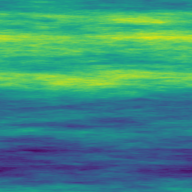
\includegraphics[interpolate=true,width=1.920000in,height=1.920000in]{random_field_anisoptropic-img0.png}}%
\end{pgfscope}%
\end{pgfpicture}%
\makeatother%
\endgroup%

    \caption{An anisotropic random field.}
    % \vspace{-10pt}
    \label{fig:ranom_field_anisotropic}
\end{wrapfigure}


% \begin{example}[White noise]
%     If the covariance is zero, we get white noise. If the covariance is one, the whole space has one degree of freedom so to speak and will have one random color.
% \end{example}
% We have a result by Loeve 
% \begin{theorem}[Loeve]
%     $k$ corresponds to the covariance of a Gaussian process if and only if $k$ is a positive semi-definite function, i.e.
%     \[
%         \sum_{i=0}^{n} \sum_{j=0}^{n} \alpha_{i} \alpha_{j} k(x_{i},x_{j}) \geq 0
%     \]
%     for all \( n \in \mathbb{N}, x_{i} \in \mathcal{X}, \alpha_{i} \in \mathbb{R} \).
% \end{theorem}

\begin{definition}[Strict Stationarity]\index{stationarity!strict}

    A stochastic process \( \{X(t)\}_{t \in T} \) is called \textit{strictly stationary} if for all \( k \geq 1 \), all \( (t_{1}, \dots t_{k}) \) in \( T^{k} \), the probability distribution of the random vector 
    \[
        (X(t_{1}+h), \dots, X(t_{k}+h))
    \]
    is independent of \( h \in T \), with \( h \in T \) such that \( t_{1}+h, \dots, t_{k}+h \in T\).
\end{definition}
%
\begin{definition}[Second Order Stochastic Process]\index{second order process}
    A measureable stochastic process \(\{X_{t}\}\) satisfying the condition
    \[
        \E\left[ \lvert X_{t} \rvert^2 \right] < \infty
    \]
    for all $t \in T$ is called a \textit{second order} stochastic process
\end{definition}
%
\begin{definition}[Weak Stationarity]\index{stationarity!weak}
    A second order stochastic process \(\{X_{t}\}\) with mean \(\mu_{X}(t)\) and covariance \( \Gamma_{X}(t,s) \) at \( t,s \in T \) is called \textit{weakly stationary}, if \( \mu_{X} \) is constant and \( \Gamma_{X}(t,s) \) is a function of \( t-s \) only.
\end{definition}

A process is called \textit{isotropic}\index{isotropy} if its covariance function \( \Gamma(t,s) \) is only a function of the distance \( \lvert t-s \rvert \). An example of when this condition is not met is shown in \cref{fig:ranom_field_anisotropic}

\begin{theorem}[Stationarity Equivalence]\index{stationarity!equivalence}
    For Gaussian processes on \( T = \mathbb{R}^{d} \), $d \in \mathbb{N}$ the concepts of weak and strict stationarity coincide.
\end{theorem}

\begin{proof}
    Strict stationarity implies weak stationarity trivially.
    For the other direction note that the mean and covariance functions completely characterize the finite dimensional distributions, since these are normal distributions.
\end{proof}
% (https://gpss.cc/gpss21/slides/Heinonen2021.pdf Page 10).
% \textcolor{red}{Do I want the following sentence?}
% In many physical domains random fields arise as sums of random waves. Their spacial interaction is understandably better characterized in the frequency domain. The following spectral theorem gives some insights into the connection between covariance functions and spectral densities. 
\begin{figure}[b]
    \centering
    %% Creator: Matplotlib, PGF backend
%%
%% To include the figure in your LaTeX document, write
%%   \input{<filename>.pgf}
%%
%% Make sure the required packages are loaded in your preamble
%%   \usepackage{pgf}
%%
%% Also ensure that all the required font packages are loaded; for instance,
%% the lmodern package is sometimes necessary when using math font.
%%   \usepackage{lmodern}
%%
%% Figures using additional raster images can only be included by \input if
%% they are in the same directory as the main LaTeX file. For loading figures
%% from other directories you can use the `import` package
%%   \usepackage{import}
%%
%% and then include the figures with
%%   \import{<path to file>}{<filename>.pgf}
%%
%% Matplotlib used the following preamble
%%   \def\mathdefault#1{#1}
%%   \everymath=\expandafter{\the\everymath\displaystyle}
%%   \usepackage[T1]{fontenc}
%%   \usepackage{siunitx}
%%   \usepackage{amssymb}
%%   \usepackage{amsmath}
%%   \makeatletter\@ifpackageloaded{underscore}{}{\usepackage[strings]{underscore}}\makeatother
%%
\begingroup%
\makeatletter%
\begin{pgfpicture}%
\pgfpathrectangle{\pgfpointorigin}{\pgfqpoint{1.736553in}{1.736553in}}%
\pgfusepath{use as bounding box, clip}%
\begin{pgfscope}%
\pgfsetbuttcap%
\pgfsetmiterjoin%
\definecolor{currentfill}{rgb}{1.000000,1.000000,1.000000}%
\pgfsetfillcolor{currentfill}%
\pgfsetlinewidth{0.000000pt}%
\definecolor{currentstroke}{rgb}{1.000000,1.000000,1.000000}%
\pgfsetstrokecolor{currentstroke}%
\pgfsetdash{}{0pt}%
\pgfpathmoveto{\pgfqpoint{0.000000in}{0.000000in}}%
\pgfpathlineto{\pgfqpoint{1.736553in}{0.000000in}}%
\pgfpathlineto{\pgfqpoint{1.736553in}{1.736553in}}%
\pgfpathlineto{\pgfqpoint{0.000000in}{1.736553in}}%
\pgfpathlineto{\pgfqpoint{0.000000in}{0.000000in}}%
\pgfpathclose%
\pgfusepath{fill}%
\end{pgfscope}%
\begin{pgfscope}%
\pgfsetbuttcap%
\pgfsetmiterjoin%
\definecolor{currentfill}{rgb}{1.000000,1.000000,1.000000}%
\pgfsetfillcolor{currentfill}%
\pgfsetlinewidth{0.000000pt}%
\definecolor{currentstroke}{rgb}{0.000000,0.000000,0.000000}%
\pgfsetstrokecolor{currentstroke}%
\pgfsetstrokeopacity{0.000000}%
\pgfsetdash{}{0pt}%
\pgfpathmoveto{\pgfqpoint{0.000000in}{0.000000in}}%
\pgfpathlineto{\pgfqpoint{1.736553in}{0.000000in}}%
\pgfpathlineto{\pgfqpoint{1.736553in}{1.736553in}}%
\pgfpathlineto{\pgfqpoint{0.000000in}{1.736553in}}%
\pgfpathlineto{\pgfqpoint{0.000000in}{0.000000in}}%
\pgfpathclose%
\pgfusepath{fill}%
\end{pgfscope}%
\begin{pgfscope}%
\pgfpathrectangle{\pgfqpoint{0.000000in}{0.000000in}}{\pgfqpoint{1.736553in}{1.736553in}}%
\pgfusepath{clip}%
\pgfsetrectcap%
\pgfsetroundjoin%
\pgfsetlinewidth{1.505625pt}%
\definecolor{currentstroke}{rgb}{1.000000,0.745098,0.043137}%
\pgfsetstrokecolor{currentstroke}%
\pgfsetdash{}{0pt}%
\pgfpathmoveto{\pgfqpoint{0.078934in}{0.597354in}}%
\pgfpathlineto{\pgfqpoint{0.094881in}{0.572819in}}%
\pgfpathlineto{\pgfqpoint{0.110827in}{0.523886in}}%
\pgfpathlineto{\pgfqpoint{0.126773in}{0.541530in}}%
\pgfpathlineto{\pgfqpoint{0.142719in}{0.555154in}}%
\pgfpathlineto{\pgfqpoint{0.158666in}{0.540930in}}%
\pgfpathlineto{\pgfqpoint{0.174612in}{0.423781in}}%
\pgfpathlineto{\pgfqpoint{0.190558in}{0.508756in}}%
\pgfpathlineto{\pgfqpoint{0.206505in}{0.383405in}}%
\pgfpathlineto{\pgfqpoint{0.222451in}{0.530588in}}%
\pgfpathlineto{\pgfqpoint{0.238397in}{0.507149in}}%
\pgfpathlineto{\pgfqpoint{0.254344in}{0.473371in}}%
\pgfpathlineto{\pgfqpoint{0.270290in}{0.447025in}}%
\pgfpathlineto{\pgfqpoint{0.286236in}{0.583090in}}%
\pgfpathlineto{\pgfqpoint{0.302183in}{0.540300in}}%
\pgfpathlineto{\pgfqpoint{0.318129in}{0.472239in}}%
\pgfpathlineto{\pgfqpoint{0.334075in}{0.466494in}}%
\pgfpathlineto{\pgfqpoint{0.350021in}{0.335508in}}%
\pgfpathlineto{\pgfqpoint{0.365968in}{0.372966in}}%
\pgfpathlineto{\pgfqpoint{0.381914in}{0.390692in}}%
\pgfpathlineto{\pgfqpoint{0.397860in}{0.388688in}}%
\pgfpathlineto{\pgfqpoint{0.413807in}{0.439716in}}%
\pgfpathlineto{\pgfqpoint{0.429753in}{0.443796in}}%
\pgfpathlineto{\pgfqpoint{0.445699in}{0.684593in}}%
\pgfpathlineto{\pgfqpoint{0.461646in}{0.677109in}}%
\pgfpathlineto{\pgfqpoint{0.477592in}{0.763308in}}%
\pgfpathlineto{\pgfqpoint{0.493538in}{0.803882in}}%
\pgfpathlineto{\pgfqpoint{0.509485in}{0.728573in}}%
\pgfpathlineto{\pgfqpoint{0.525431in}{0.658339in}}%
\pgfpathlineto{\pgfqpoint{0.541377in}{0.597465in}}%
\pgfpathlineto{\pgfqpoint{0.557323in}{0.678167in}}%
\pgfpathlineto{\pgfqpoint{0.573270in}{0.803808in}}%
\pgfpathlineto{\pgfqpoint{0.589216in}{0.957796in}}%
\pgfpathlineto{\pgfqpoint{0.605162in}{0.955543in}}%
\pgfpathlineto{\pgfqpoint{0.621109in}{0.944501in}}%
\pgfpathlineto{\pgfqpoint{0.637055in}{0.959784in}}%
\pgfpathlineto{\pgfqpoint{0.653001in}{0.858692in}}%
\pgfpathlineto{\pgfqpoint{0.668948in}{0.816514in}}%
\pgfpathlineto{\pgfqpoint{0.684894in}{0.743290in}}%
\pgfpathlineto{\pgfqpoint{0.700840in}{0.884732in}}%
\pgfpathlineto{\pgfqpoint{0.716787in}{0.910608in}}%
\pgfpathlineto{\pgfqpoint{0.732733in}{0.924974in}}%
\pgfpathlineto{\pgfqpoint{0.748679in}{0.981079in}}%
\pgfpathlineto{\pgfqpoint{0.764625in}{0.975342in}}%
\pgfpathlineto{\pgfqpoint{0.780572in}{1.054578in}}%
\pgfpathlineto{\pgfqpoint{0.796518in}{0.931943in}}%
\pgfpathlineto{\pgfqpoint{0.812464in}{0.987974in}}%
\pgfpathlineto{\pgfqpoint{0.828411in}{0.899395in}}%
\pgfpathlineto{\pgfqpoint{0.844357in}{0.884652in}}%
\pgfpathlineto{\pgfqpoint{0.860303in}{0.952260in}}%
\pgfpathlineto{\pgfqpoint{0.876250in}{0.921470in}}%
\pgfpathlineto{\pgfqpoint{0.892196in}{0.952062in}}%
\pgfpathlineto{\pgfqpoint{0.908142in}{0.876299in}}%
\pgfpathlineto{\pgfqpoint{0.924089in}{0.824040in}}%
\pgfpathlineto{\pgfqpoint{0.940035in}{0.824115in}}%
\pgfpathlineto{\pgfqpoint{0.955981in}{0.729242in}}%
\pgfpathlineto{\pgfqpoint{0.971928in}{0.680483in}}%
\pgfpathlineto{\pgfqpoint{0.987874in}{0.643527in}}%
\pgfpathlineto{\pgfqpoint{1.003820in}{0.773837in}}%
\pgfpathlineto{\pgfqpoint{1.019766in}{0.782563in}}%
\pgfpathlineto{\pgfqpoint{1.035713in}{0.707945in}}%
\pgfpathlineto{\pgfqpoint{1.051659in}{0.671844in}}%
\pgfpathlineto{\pgfqpoint{1.067605in}{0.678028in}}%
\pgfpathlineto{\pgfqpoint{1.083552in}{0.714294in}}%
\pgfpathlineto{\pgfqpoint{1.099498in}{0.709146in}}%
\pgfpathlineto{\pgfqpoint{1.115444in}{0.594807in}}%
\pgfpathlineto{\pgfqpoint{1.131391in}{0.443070in}}%
\pgfpathlineto{\pgfqpoint{1.147337in}{0.422680in}}%
\pgfpathlineto{\pgfqpoint{1.163283in}{0.605446in}}%
\pgfpathlineto{\pgfqpoint{1.179230in}{0.434094in}}%
\pgfpathlineto{\pgfqpoint{1.195176in}{0.236813in}}%
\pgfpathlineto{\pgfqpoint{1.211122in}{0.217593in}}%
\pgfpathlineto{\pgfqpoint{1.227068in}{0.157423in}}%
\pgfpathlineto{\pgfqpoint{1.243015in}{0.412849in}}%
\pgfpathlineto{\pgfqpoint{1.258961in}{0.500857in}}%
\pgfpathlineto{\pgfqpoint{1.274907in}{0.560561in}}%
\pgfpathlineto{\pgfqpoint{1.290854in}{0.502796in}}%
\pgfpathlineto{\pgfqpoint{1.306800in}{0.376484in}}%
\pgfpathlineto{\pgfqpoint{1.322746in}{0.258868in}}%
\pgfpathlineto{\pgfqpoint{1.338693in}{0.273022in}}%
\pgfpathlineto{\pgfqpoint{1.354639in}{0.466646in}}%
\pgfpathlineto{\pgfqpoint{1.370585in}{0.582374in}}%
\pgfpathlineto{\pgfqpoint{1.386532in}{0.645853in}}%
\pgfpathlineto{\pgfqpoint{1.402478in}{0.828005in}}%
\pgfpathlineto{\pgfqpoint{1.418424in}{0.858518in}}%
\pgfpathlineto{\pgfqpoint{1.434370in}{0.803388in}}%
\pgfpathlineto{\pgfqpoint{1.450317in}{0.779115in}}%
\pgfpathlineto{\pgfqpoint{1.466263in}{0.870217in}}%
\pgfpathlineto{\pgfqpoint{1.482209in}{0.876953in}}%
\pgfpathlineto{\pgfqpoint{1.498156in}{0.905919in}}%
\pgfpathlineto{\pgfqpoint{1.514102in}{0.872603in}}%
\pgfpathlineto{\pgfqpoint{1.530048in}{0.914796in}}%
\pgfpathlineto{\pgfqpoint{1.545995in}{1.115195in}}%
\pgfpathlineto{\pgfqpoint{1.561941in}{1.288556in}}%
\pgfpathlineto{\pgfqpoint{1.577887in}{1.138474in}}%
\pgfpathlineto{\pgfqpoint{1.593834in}{1.322962in}}%
\pgfpathlineto{\pgfqpoint{1.609780in}{1.409074in}}%
\pgfpathlineto{\pgfqpoint{1.625726in}{1.501723in}}%
\pgfpathlineto{\pgfqpoint{1.641672in}{1.508594in}}%
\pgfpathlineto{\pgfqpoint{1.657619in}{1.421900in}}%
\pgfusepath{stroke}%
\end{pgfscope}%
\begin{pgfscope}%
\pgfpathrectangle{\pgfqpoint{0.000000in}{0.000000in}}{\pgfqpoint{1.736553in}{1.736553in}}%
\pgfusepath{clip}%
\pgfsetrectcap%
\pgfsetroundjoin%
\pgfsetlinewidth{1.505625pt}%
\definecolor{currentstroke}{rgb}{0.984314,0.337255,0.027451}%
\pgfsetstrokecolor{currentstroke}%
\pgfsetdash{}{0pt}%
\pgfpathmoveto{\pgfqpoint{0.078934in}{0.798942in}}%
\pgfpathlineto{\pgfqpoint{0.094881in}{0.920122in}}%
\pgfpathlineto{\pgfqpoint{0.110827in}{0.833388in}}%
\pgfpathlineto{\pgfqpoint{0.126773in}{0.934435in}}%
\pgfpathlineto{\pgfqpoint{0.142719in}{0.927345in}}%
\pgfpathlineto{\pgfqpoint{0.158666in}{1.112003in}}%
\pgfpathlineto{\pgfqpoint{0.174612in}{1.191900in}}%
\pgfpathlineto{\pgfqpoint{0.190558in}{1.229548in}}%
\pgfpathlineto{\pgfqpoint{0.206505in}{1.180584in}}%
\pgfpathlineto{\pgfqpoint{0.222451in}{1.128798in}}%
\pgfpathlineto{\pgfqpoint{0.238397in}{1.305087in}}%
\pgfpathlineto{\pgfqpoint{0.254344in}{1.269954in}}%
\pgfpathlineto{\pgfqpoint{0.270290in}{1.185360in}}%
\pgfpathlineto{\pgfqpoint{0.286236in}{1.271441in}}%
\pgfpathlineto{\pgfqpoint{0.302183in}{1.088432in}}%
\pgfpathlineto{\pgfqpoint{0.318129in}{1.057050in}}%
\pgfpathlineto{\pgfqpoint{0.334075in}{0.915948in}}%
\pgfpathlineto{\pgfqpoint{0.350021in}{1.031808in}}%
\pgfpathlineto{\pgfqpoint{0.365968in}{0.972760in}}%
\pgfpathlineto{\pgfqpoint{0.381914in}{1.051939in}}%
\pgfpathlineto{\pgfqpoint{0.397860in}{1.097358in}}%
\pgfpathlineto{\pgfqpoint{0.413807in}{1.105391in}}%
\pgfpathlineto{\pgfqpoint{0.429753in}{0.911435in}}%
\pgfpathlineto{\pgfqpoint{0.445699in}{1.043790in}}%
\pgfpathlineto{\pgfqpoint{0.461646in}{0.987670in}}%
\pgfpathlineto{\pgfqpoint{0.477592in}{0.899375in}}%
\pgfpathlineto{\pgfqpoint{0.493538in}{0.765688in}}%
\pgfpathlineto{\pgfqpoint{0.509485in}{0.839864in}}%
\pgfpathlineto{\pgfqpoint{0.525431in}{0.876479in}}%
\pgfpathlineto{\pgfqpoint{0.541377in}{0.887176in}}%
\pgfpathlineto{\pgfqpoint{0.557323in}{0.841167in}}%
\pgfpathlineto{\pgfqpoint{0.573270in}{0.835870in}}%
\pgfpathlineto{\pgfqpoint{0.589216in}{0.821962in}}%
\pgfpathlineto{\pgfqpoint{0.605162in}{0.933747in}}%
\pgfpathlineto{\pgfqpoint{0.621109in}{1.034096in}}%
\pgfpathlineto{\pgfqpoint{0.637055in}{1.079633in}}%
\pgfpathlineto{\pgfqpoint{0.653001in}{1.063012in}}%
\pgfpathlineto{\pgfqpoint{0.668948in}{1.252042in}}%
\pgfpathlineto{\pgfqpoint{0.684894in}{1.219583in}}%
\pgfpathlineto{\pgfqpoint{0.700840in}{1.087553in}}%
\pgfpathlineto{\pgfqpoint{0.716787in}{0.986535in}}%
\pgfpathlineto{\pgfqpoint{0.732733in}{0.860421in}}%
\pgfpathlineto{\pgfqpoint{0.748679in}{0.699626in}}%
\pgfpathlineto{\pgfqpoint{0.764625in}{0.679939in}}%
\pgfpathlineto{\pgfqpoint{0.780572in}{0.564763in}}%
\pgfpathlineto{\pgfqpoint{0.796518in}{0.515891in}}%
\pgfpathlineto{\pgfqpoint{0.812464in}{0.499956in}}%
\pgfpathlineto{\pgfqpoint{0.828411in}{0.376758in}}%
\pgfpathlineto{\pgfqpoint{0.844357in}{0.236002in}}%
\pgfpathlineto{\pgfqpoint{0.860303in}{0.212152in}}%
\pgfpathlineto{\pgfqpoint{0.876250in}{0.129080in}}%
\pgfpathlineto{\pgfqpoint{0.892196in}{0.114616in}}%
\pgfpathlineto{\pgfqpoint{0.908142in}{0.146088in}}%
\pgfpathlineto{\pgfqpoint{0.924089in}{0.078934in}}%
\pgfpathlineto{\pgfqpoint{0.940035in}{0.102285in}}%
\pgfpathlineto{\pgfqpoint{0.955981in}{0.198688in}}%
\pgfpathlineto{\pgfqpoint{0.971928in}{0.226882in}}%
\pgfpathlineto{\pgfqpoint{0.987874in}{0.314157in}}%
\pgfpathlineto{\pgfqpoint{1.003820in}{0.242413in}}%
\pgfpathlineto{\pgfqpoint{1.019766in}{0.312075in}}%
\pgfpathlineto{\pgfqpoint{1.035713in}{0.315072in}}%
\pgfpathlineto{\pgfqpoint{1.051659in}{0.213218in}}%
\pgfpathlineto{\pgfqpoint{1.067605in}{0.125709in}}%
\pgfpathlineto{\pgfqpoint{1.083552in}{0.147907in}}%
\pgfpathlineto{\pgfqpoint{1.099498in}{0.352521in}}%
\pgfpathlineto{\pgfqpoint{1.115444in}{0.258638in}}%
\pgfpathlineto{\pgfqpoint{1.131391in}{0.284158in}}%
\pgfpathlineto{\pgfqpoint{1.147337in}{0.287550in}}%
\pgfpathlineto{\pgfqpoint{1.163283in}{0.329746in}}%
\pgfpathlineto{\pgfqpoint{1.179230in}{0.316850in}}%
\pgfpathlineto{\pgfqpoint{1.195176in}{0.387564in}}%
\pgfpathlineto{\pgfqpoint{1.211122in}{0.321173in}}%
\pgfpathlineto{\pgfqpoint{1.227068in}{0.394013in}}%
\pgfpathlineto{\pgfqpoint{1.243015in}{0.705268in}}%
\pgfpathlineto{\pgfqpoint{1.258961in}{0.623876in}}%
\pgfpathlineto{\pgfqpoint{1.274907in}{0.786438in}}%
\pgfpathlineto{\pgfqpoint{1.290854in}{0.804252in}}%
\pgfpathlineto{\pgfqpoint{1.306800in}{0.722137in}}%
\pgfpathlineto{\pgfqpoint{1.322746in}{0.778773in}}%
\pgfpathlineto{\pgfqpoint{1.338693in}{0.914040in}}%
\pgfpathlineto{\pgfqpoint{1.354639in}{1.023506in}}%
\pgfpathlineto{\pgfqpoint{1.370585in}{0.935107in}}%
\pgfpathlineto{\pgfqpoint{1.386532in}{0.875209in}}%
\pgfpathlineto{\pgfqpoint{1.402478in}{0.860306in}}%
\pgfpathlineto{\pgfqpoint{1.418424in}{0.902711in}}%
\pgfpathlineto{\pgfqpoint{1.434370in}{0.870994in}}%
\pgfpathlineto{\pgfqpoint{1.450317in}{0.773331in}}%
\pgfpathlineto{\pgfqpoint{1.466263in}{0.712112in}}%
\pgfpathlineto{\pgfqpoint{1.482209in}{0.834711in}}%
\pgfpathlineto{\pgfqpoint{1.498156in}{0.733362in}}%
\pgfpathlineto{\pgfqpoint{1.514102in}{0.589783in}}%
\pgfpathlineto{\pgfqpoint{1.530048in}{0.416617in}}%
\pgfpathlineto{\pgfqpoint{1.545995in}{0.529055in}}%
\pgfpathlineto{\pgfqpoint{1.561941in}{0.515840in}}%
\pgfpathlineto{\pgfqpoint{1.577887in}{0.540384in}}%
\pgfpathlineto{\pgfqpoint{1.593834in}{0.664321in}}%
\pgfpathlineto{\pgfqpoint{1.609780in}{0.726687in}}%
\pgfpathlineto{\pgfqpoint{1.625726in}{0.826325in}}%
\pgfpathlineto{\pgfqpoint{1.641672in}{0.798123in}}%
\pgfpathlineto{\pgfqpoint{1.657619in}{0.859115in}}%
\pgfusepath{stroke}%
\end{pgfscope}%
\begin{pgfscope}%
\pgfpathrectangle{\pgfqpoint{0.000000in}{0.000000in}}{\pgfqpoint{1.736553in}{1.736553in}}%
\pgfusepath{clip}%
\pgfsetrectcap%
\pgfsetroundjoin%
\pgfsetlinewidth{1.505625pt}%
\definecolor{currentstroke}{rgb}{1.000000,0.000000,0.431373}%
\pgfsetstrokecolor{currentstroke}%
\pgfsetdash{}{0pt}%
\pgfpathmoveto{\pgfqpoint{0.078934in}{0.914283in}}%
\pgfpathlineto{\pgfqpoint{0.094881in}{0.759890in}}%
\pgfpathlineto{\pgfqpoint{0.110827in}{0.762467in}}%
\pgfpathlineto{\pgfqpoint{0.126773in}{0.810402in}}%
\pgfpathlineto{\pgfqpoint{0.142719in}{0.804461in}}%
\pgfpathlineto{\pgfqpoint{0.158666in}{0.748231in}}%
\pgfpathlineto{\pgfqpoint{0.174612in}{0.752133in}}%
\pgfpathlineto{\pgfqpoint{0.190558in}{0.847007in}}%
\pgfpathlineto{\pgfqpoint{0.206505in}{0.795824in}}%
\pgfpathlineto{\pgfqpoint{0.222451in}{0.864590in}}%
\pgfpathlineto{\pgfqpoint{0.238397in}{0.845323in}}%
\pgfpathlineto{\pgfqpoint{0.254344in}{0.949608in}}%
\pgfpathlineto{\pgfqpoint{0.270290in}{1.050594in}}%
\pgfpathlineto{\pgfqpoint{0.286236in}{1.148055in}}%
\pgfpathlineto{\pgfqpoint{0.302183in}{1.091956in}}%
\pgfpathlineto{\pgfqpoint{0.318129in}{0.945966in}}%
\pgfpathlineto{\pgfqpoint{0.334075in}{1.035360in}}%
\pgfpathlineto{\pgfqpoint{0.350021in}{1.140232in}}%
\pgfpathlineto{\pgfqpoint{0.365968in}{1.142261in}}%
\pgfpathlineto{\pgfqpoint{0.381914in}{1.215936in}}%
\pgfpathlineto{\pgfqpoint{0.397860in}{1.238661in}}%
\pgfpathlineto{\pgfqpoint{0.413807in}{1.198636in}}%
\pgfpathlineto{\pgfqpoint{0.429753in}{1.184471in}}%
\pgfpathlineto{\pgfqpoint{0.445699in}{1.171784in}}%
\pgfpathlineto{\pgfqpoint{0.461646in}{1.144104in}}%
\pgfpathlineto{\pgfqpoint{0.477592in}{1.080395in}}%
\pgfpathlineto{\pgfqpoint{0.493538in}{1.028049in}}%
\pgfpathlineto{\pgfqpoint{0.509485in}{0.988106in}}%
\pgfpathlineto{\pgfqpoint{0.525431in}{1.019079in}}%
\pgfpathlineto{\pgfqpoint{0.541377in}{1.159316in}}%
\pgfpathlineto{\pgfqpoint{0.557323in}{1.164618in}}%
\pgfpathlineto{\pgfqpoint{0.573270in}{1.096027in}}%
\pgfpathlineto{\pgfqpoint{0.589216in}{1.062091in}}%
\pgfpathlineto{\pgfqpoint{0.605162in}{1.107313in}}%
\pgfpathlineto{\pgfqpoint{0.621109in}{1.260780in}}%
\pgfpathlineto{\pgfqpoint{0.637055in}{1.310391in}}%
\pgfpathlineto{\pgfqpoint{0.653001in}{1.255074in}}%
\pgfpathlineto{\pgfqpoint{0.668948in}{1.126837in}}%
\pgfpathlineto{\pgfqpoint{0.684894in}{1.130008in}}%
\pgfpathlineto{\pgfqpoint{0.700840in}{1.224745in}}%
\pgfpathlineto{\pgfqpoint{0.716787in}{1.250641in}}%
\pgfpathlineto{\pgfqpoint{0.732733in}{1.172528in}}%
\pgfpathlineto{\pgfqpoint{0.748679in}{1.260710in}}%
\pgfpathlineto{\pgfqpoint{0.764625in}{1.214870in}}%
\pgfpathlineto{\pgfqpoint{0.780572in}{1.330452in}}%
\pgfpathlineto{\pgfqpoint{0.796518in}{1.484145in}}%
\pgfpathlineto{\pgfqpoint{0.812464in}{1.324183in}}%
\pgfpathlineto{\pgfqpoint{0.828411in}{1.339245in}}%
\pgfpathlineto{\pgfqpoint{0.844357in}{1.317734in}}%
\pgfpathlineto{\pgfqpoint{0.860303in}{1.121460in}}%
\pgfpathlineto{\pgfqpoint{0.876250in}{1.185619in}}%
\pgfpathlineto{\pgfqpoint{0.892196in}{1.278935in}}%
\pgfpathlineto{\pgfqpoint{0.908142in}{1.331868in}}%
\pgfpathlineto{\pgfqpoint{0.924089in}{1.344835in}}%
\pgfpathlineto{\pgfqpoint{0.940035in}{1.307172in}}%
\pgfpathlineto{\pgfqpoint{0.955981in}{1.367194in}}%
\pgfpathlineto{\pgfqpoint{0.971928in}{1.267012in}}%
\pgfpathlineto{\pgfqpoint{0.987874in}{1.287025in}}%
\pgfpathlineto{\pgfqpoint{1.003820in}{1.158077in}}%
\pgfpathlineto{\pgfqpoint{1.019766in}{1.206715in}}%
\pgfpathlineto{\pgfqpoint{1.035713in}{1.106788in}}%
\pgfpathlineto{\pgfqpoint{1.051659in}{1.229908in}}%
\pgfpathlineto{\pgfqpoint{1.067605in}{1.312622in}}%
\pgfpathlineto{\pgfqpoint{1.083552in}{1.249083in}}%
\pgfpathlineto{\pgfqpoint{1.099498in}{1.299443in}}%
\pgfpathlineto{\pgfqpoint{1.115444in}{1.243921in}}%
\pgfpathlineto{\pgfqpoint{1.131391in}{1.229226in}}%
\pgfpathlineto{\pgfqpoint{1.147337in}{1.070590in}}%
\pgfpathlineto{\pgfqpoint{1.163283in}{1.002885in}}%
\pgfpathlineto{\pgfqpoint{1.179230in}{0.858755in}}%
\pgfpathlineto{\pgfqpoint{1.195176in}{0.885790in}}%
\pgfpathlineto{\pgfqpoint{1.211122in}{0.650841in}}%
\pgfpathlineto{\pgfqpoint{1.227068in}{0.780285in}}%
\pgfpathlineto{\pgfqpoint{1.243015in}{0.895476in}}%
\pgfpathlineto{\pgfqpoint{1.258961in}{0.701046in}}%
\pgfpathlineto{\pgfqpoint{1.274907in}{0.816009in}}%
\pgfpathlineto{\pgfqpoint{1.290854in}{0.850389in}}%
\pgfpathlineto{\pgfqpoint{1.306800in}{0.872423in}}%
\pgfpathlineto{\pgfqpoint{1.322746in}{0.862225in}}%
\pgfpathlineto{\pgfqpoint{1.338693in}{0.932260in}}%
\pgfpathlineto{\pgfqpoint{1.354639in}{0.837747in}}%
\pgfpathlineto{\pgfqpoint{1.370585in}{0.858652in}}%
\pgfpathlineto{\pgfqpoint{1.386532in}{0.689382in}}%
\pgfpathlineto{\pgfqpoint{1.402478in}{0.722323in}}%
\pgfpathlineto{\pgfqpoint{1.418424in}{0.744268in}}%
\pgfpathlineto{\pgfqpoint{1.434370in}{0.835945in}}%
\pgfpathlineto{\pgfqpoint{1.450317in}{0.933643in}}%
\pgfpathlineto{\pgfqpoint{1.466263in}{0.895979in}}%
\pgfpathlineto{\pgfqpoint{1.482209in}{0.907833in}}%
\pgfpathlineto{\pgfqpoint{1.498156in}{0.966746in}}%
\pgfpathlineto{\pgfqpoint{1.514102in}{0.954813in}}%
\pgfpathlineto{\pgfqpoint{1.530048in}{0.949608in}}%
\pgfpathlineto{\pgfqpoint{1.545995in}{1.022315in}}%
\pgfpathlineto{\pgfqpoint{1.561941in}{1.197833in}}%
\pgfpathlineto{\pgfqpoint{1.577887in}{1.105779in}}%
\pgfpathlineto{\pgfqpoint{1.593834in}{1.102393in}}%
\pgfpathlineto{\pgfqpoint{1.609780in}{1.181239in}}%
\pgfpathlineto{\pgfqpoint{1.625726in}{1.119112in}}%
\pgfpathlineto{\pgfqpoint{1.641672in}{1.345942in}}%
\pgfpathlineto{\pgfqpoint{1.657619in}{1.180953in}}%
\pgfusepath{stroke}%
\end{pgfscope}%
\begin{pgfscope}%
\pgfpathrectangle{\pgfqpoint{0.000000in}{0.000000in}}{\pgfqpoint{1.736553in}{1.736553in}}%
\pgfusepath{clip}%
\pgfsetrectcap%
\pgfsetroundjoin%
\pgfsetlinewidth{1.505625pt}%
\definecolor{currentstroke}{rgb}{0.513725,0.219608,0.925490}%
\pgfsetstrokecolor{currentstroke}%
\pgfsetdash{}{0pt}%
\pgfpathmoveto{\pgfqpoint{0.078934in}{0.801081in}}%
\pgfpathlineto{\pgfqpoint{0.094881in}{0.856508in}}%
\pgfpathlineto{\pgfqpoint{0.110827in}{0.703491in}}%
\pgfpathlineto{\pgfqpoint{0.126773in}{0.777527in}}%
\pgfpathlineto{\pgfqpoint{0.142719in}{0.880366in}}%
\pgfpathlineto{\pgfqpoint{0.158666in}{1.015537in}}%
\pgfpathlineto{\pgfqpoint{0.174612in}{1.029396in}}%
\pgfpathlineto{\pgfqpoint{0.190558in}{1.011373in}}%
\pgfpathlineto{\pgfqpoint{0.206505in}{1.126453in}}%
\pgfpathlineto{\pgfqpoint{0.222451in}{1.096157in}}%
\pgfpathlineto{\pgfqpoint{0.238397in}{1.200942in}}%
\pgfpathlineto{\pgfqpoint{0.254344in}{1.188402in}}%
\pgfpathlineto{\pgfqpoint{0.270290in}{1.174694in}}%
\pgfpathlineto{\pgfqpoint{0.286236in}{1.153127in}}%
\pgfpathlineto{\pgfqpoint{0.302183in}{1.042623in}}%
\pgfpathlineto{\pgfqpoint{0.318129in}{1.264589in}}%
\pgfpathlineto{\pgfqpoint{0.334075in}{1.161412in}}%
\pgfpathlineto{\pgfqpoint{0.350021in}{1.097906in}}%
\pgfpathlineto{\pgfqpoint{0.365968in}{0.887998in}}%
\pgfpathlineto{\pgfqpoint{0.381914in}{0.945005in}}%
\pgfpathlineto{\pgfqpoint{0.397860in}{1.015138in}}%
\pgfpathlineto{\pgfqpoint{0.413807in}{1.098870in}}%
\pgfpathlineto{\pgfqpoint{0.429753in}{1.008025in}}%
\pgfpathlineto{\pgfqpoint{0.445699in}{0.970493in}}%
\pgfpathlineto{\pgfqpoint{0.461646in}{0.803162in}}%
\pgfpathlineto{\pgfqpoint{0.477592in}{0.806862in}}%
\pgfpathlineto{\pgfqpoint{0.493538in}{0.755046in}}%
\pgfpathlineto{\pgfqpoint{0.509485in}{0.955592in}}%
\pgfpathlineto{\pgfqpoint{0.525431in}{0.919179in}}%
\pgfpathlineto{\pgfqpoint{0.541377in}{0.829906in}}%
\pgfpathlineto{\pgfqpoint{0.557323in}{0.771184in}}%
\pgfpathlineto{\pgfqpoint{0.573270in}{0.725325in}}%
\pgfpathlineto{\pgfqpoint{0.589216in}{0.609031in}}%
\pgfpathlineto{\pgfqpoint{0.605162in}{0.736792in}}%
\pgfpathlineto{\pgfqpoint{0.621109in}{0.849551in}}%
\pgfpathlineto{\pgfqpoint{0.637055in}{0.956293in}}%
\pgfpathlineto{\pgfqpoint{0.653001in}{0.983325in}}%
\pgfpathlineto{\pgfqpoint{0.668948in}{0.894786in}}%
\pgfpathlineto{\pgfqpoint{0.684894in}{0.976994in}}%
\pgfpathlineto{\pgfqpoint{0.700840in}{0.991664in}}%
\pgfpathlineto{\pgfqpoint{0.716787in}{1.137180in}}%
\pgfpathlineto{\pgfqpoint{0.732733in}{1.189801in}}%
\pgfpathlineto{\pgfqpoint{0.748679in}{1.252874in}}%
\pgfpathlineto{\pgfqpoint{0.764625in}{1.341866in}}%
\pgfpathlineto{\pgfqpoint{0.780572in}{1.403199in}}%
\pgfpathlineto{\pgfqpoint{0.796518in}{1.464474in}}%
\pgfpathlineto{\pgfqpoint{0.812464in}{1.401630in}}%
\pgfpathlineto{\pgfqpoint{0.828411in}{1.440726in}}%
\pgfpathlineto{\pgfqpoint{0.844357in}{1.356706in}}%
\pgfpathlineto{\pgfqpoint{0.860303in}{1.326471in}}%
\pgfpathlineto{\pgfqpoint{0.876250in}{1.329010in}}%
\pgfpathlineto{\pgfqpoint{0.892196in}{1.398592in}}%
\pgfpathlineto{\pgfqpoint{0.908142in}{1.397526in}}%
\pgfpathlineto{\pgfqpoint{0.924089in}{1.315933in}}%
\pgfpathlineto{\pgfqpoint{0.940035in}{1.387170in}}%
\pgfpathlineto{\pgfqpoint{0.955981in}{1.335719in}}%
\pgfpathlineto{\pgfqpoint{0.971928in}{1.408417in}}%
\pgfpathlineto{\pgfqpoint{0.987874in}{1.415123in}}%
\pgfpathlineto{\pgfqpoint{1.003820in}{1.529465in}}%
\pgfpathlineto{\pgfqpoint{1.019766in}{1.606603in}}%
\pgfpathlineto{\pgfqpoint{1.035713in}{1.438392in}}%
\pgfpathlineto{\pgfqpoint{1.051659in}{1.513729in}}%
\pgfpathlineto{\pgfqpoint{1.067605in}{1.617104in}}%
\pgfpathlineto{\pgfqpoint{1.083552in}{1.552834in}}%
\pgfpathlineto{\pgfqpoint{1.099498in}{1.477076in}}%
\pgfpathlineto{\pgfqpoint{1.115444in}{1.486820in}}%
\pgfpathlineto{\pgfqpoint{1.131391in}{1.530801in}}%
\pgfpathlineto{\pgfqpoint{1.147337in}{1.526768in}}%
\pgfpathlineto{\pgfqpoint{1.163283in}{1.451859in}}%
\pgfpathlineto{\pgfqpoint{1.179230in}{1.419316in}}%
\pgfpathlineto{\pgfqpoint{1.195176in}{1.470831in}}%
\pgfpathlineto{\pgfqpoint{1.211122in}{1.479916in}}%
\pgfpathlineto{\pgfqpoint{1.227068in}{1.481475in}}%
\pgfpathlineto{\pgfqpoint{1.243015in}{1.487022in}}%
\pgfpathlineto{\pgfqpoint{1.258961in}{1.469063in}}%
\pgfpathlineto{\pgfqpoint{1.274907in}{1.566939in}}%
\pgfpathlineto{\pgfqpoint{1.290854in}{1.657619in}}%
\pgfpathlineto{\pgfqpoint{1.306800in}{1.564765in}}%
\pgfpathlineto{\pgfqpoint{1.322746in}{1.520723in}}%
\pgfpathlineto{\pgfqpoint{1.338693in}{1.485344in}}%
\pgfpathlineto{\pgfqpoint{1.354639in}{1.414083in}}%
\pgfpathlineto{\pgfqpoint{1.370585in}{1.564525in}}%
\pgfpathlineto{\pgfqpoint{1.386532in}{1.531984in}}%
\pgfpathlineto{\pgfqpoint{1.402478in}{1.512745in}}%
\pgfpathlineto{\pgfqpoint{1.418424in}{1.360463in}}%
\pgfpathlineto{\pgfqpoint{1.434370in}{1.374369in}}%
\pgfpathlineto{\pgfqpoint{1.450317in}{1.528217in}}%
\pgfpathlineto{\pgfqpoint{1.466263in}{1.531270in}}%
\pgfpathlineto{\pgfqpoint{1.482209in}{1.618586in}}%
\pgfpathlineto{\pgfqpoint{1.498156in}{1.389914in}}%
\pgfpathlineto{\pgfqpoint{1.514102in}{1.428816in}}%
\pgfpathlineto{\pgfqpoint{1.530048in}{1.380128in}}%
\pgfpathlineto{\pgfqpoint{1.545995in}{1.396314in}}%
\pgfpathlineto{\pgfqpoint{1.561941in}{1.532668in}}%
\pgfpathlineto{\pgfqpoint{1.577887in}{1.532761in}}%
\pgfpathlineto{\pgfqpoint{1.593834in}{1.520029in}}%
\pgfpathlineto{\pgfqpoint{1.609780in}{1.418517in}}%
\pgfpathlineto{\pgfqpoint{1.625726in}{1.308956in}}%
\pgfpathlineto{\pgfqpoint{1.641672in}{1.325702in}}%
\pgfpathlineto{\pgfqpoint{1.657619in}{1.165301in}}%
\pgfusepath{stroke}%
\end{pgfscope}%
\end{pgfpicture}%
\makeatother%
\endgroup%

    %% Creator: Matplotlib, PGF backend
%%
%% To include the figure in your LaTeX document, write
%%   \input{<filename>.pgf}
%%
%% Make sure the required packages are loaded in your preamble
%%   \usepackage{pgf}
%%
%% Also ensure that all the required font packages are loaded; for instance,
%% the lmodern package is sometimes necessary when using math font.
%%   \usepackage{lmodern}
%%
%% Figures using additional raster images can only be included by \input if
%% they are in the same directory as the main LaTeX file. For loading figures
%% from other directories you can use the `import` package
%%   \usepackage{import}
%%
%% and then include the figures with
%%   \import{<path to file>}{<filename>.pgf}
%%
%% Matplotlib used the following preamble
%%   \def\mathdefault#1{#1}
%%   \everymath=\expandafter{\the\everymath\displaystyle}
%%   \usepackage[T1]{fontenc}
%%   \usepackage{siunitx}
%%   \usepackage{amssymb}
%%   \usepackage{amsmath}
%%   \makeatletter\@ifpackageloaded{underscore}{}{\usepackage[strings]{underscore}}\makeatother
%%
\begingroup%
\makeatletter%
\begin{pgfpicture}%
\pgfpathrectangle{\pgfpointorigin}{\pgfqpoint{1.736553in}{1.736553in}}%
\pgfusepath{use as bounding box, clip}%
\begin{pgfscope}%
\pgfsetbuttcap%
\pgfsetmiterjoin%
\definecolor{currentfill}{rgb}{1.000000,1.000000,1.000000}%
\pgfsetfillcolor{currentfill}%
\pgfsetlinewidth{0.000000pt}%
\definecolor{currentstroke}{rgb}{1.000000,1.000000,1.000000}%
\pgfsetstrokecolor{currentstroke}%
\pgfsetdash{}{0pt}%
\pgfpathmoveto{\pgfqpoint{0.000000in}{0.000000in}}%
\pgfpathlineto{\pgfqpoint{1.736553in}{0.000000in}}%
\pgfpathlineto{\pgfqpoint{1.736553in}{1.736553in}}%
\pgfpathlineto{\pgfqpoint{0.000000in}{1.736553in}}%
\pgfpathlineto{\pgfqpoint{0.000000in}{0.000000in}}%
\pgfpathclose%
\pgfusepath{fill}%
\end{pgfscope}%
\begin{pgfscope}%
\pgfsetbuttcap%
\pgfsetmiterjoin%
\definecolor{currentfill}{rgb}{1.000000,1.000000,1.000000}%
\pgfsetfillcolor{currentfill}%
\pgfsetlinewidth{0.000000pt}%
\definecolor{currentstroke}{rgb}{0.000000,0.000000,0.000000}%
\pgfsetstrokecolor{currentstroke}%
\pgfsetstrokeopacity{0.000000}%
\pgfsetdash{}{0pt}%
\pgfpathmoveto{\pgfqpoint{0.000000in}{0.000000in}}%
\pgfpathlineto{\pgfqpoint{1.736553in}{0.000000in}}%
\pgfpathlineto{\pgfqpoint{1.736553in}{1.736553in}}%
\pgfpathlineto{\pgfqpoint{0.000000in}{1.736553in}}%
\pgfpathlineto{\pgfqpoint{0.000000in}{0.000000in}}%
\pgfpathclose%
\pgfusepath{fill}%
\end{pgfscope}%
\begin{pgfscope}%
\pgfpathrectangle{\pgfqpoint{0.000000in}{0.000000in}}{\pgfqpoint{1.736553in}{1.736553in}}%
\pgfusepath{clip}%
\pgfsetrectcap%
\pgfsetroundjoin%
\pgfsetlinewidth{1.505625pt}%
\definecolor{currentstroke}{rgb}{1.000000,0.745098,0.043137}%
\pgfsetstrokecolor{currentstroke}%
\pgfsetdash{}{0pt}%
\pgfpathmoveto{\pgfqpoint{0.078934in}{0.179801in}}%
\pgfpathlineto{\pgfqpoint{0.094881in}{0.195062in}}%
\pgfpathlineto{\pgfqpoint{0.110827in}{0.216311in}}%
\pgfpathlineto{\pgfqpoint{0.126773in}{0.218788in}}%
\pgfpathlineto{\pgfqpoint{0.142719in}{0.220642in}}%
\pgfpathlineto{\pgfqpoint{0.158666in}{0.233616in}}%
\pgfpathlineto{\pgfqpoint{0.174612in}{0.261880in}}%
\pgfpathlineto{\pgfqpoint{0.190558in}{0.278933in}}%
\pgfpathlineto{\pgfqpoint{0.206505in}{0.307123in}}%
\pgfpathlineto{\pgfqpoint{0.222451in}{0.323073in}}%
\pgfpathlineto{\pgfqpoint{0.238397in}{0.329202in}}%
\pgfpathlineto{\pgfqpoint{0.254344in}{0.342146in}}%
\pgfpathlineto{\pgfqpoint{0.270290in}{0.357922in}}%
\pgfpathlineto{\pgfqpoint{0.286236in}{0.381775in}}%
\pgfpathlineto{\pgfqpoint{0.302183in}{0.427759in}}%
\pgfpathlineto{\pgfqpoint{0.318129in}{0.481641in}}%
\pgfpathlineto{\pgfqpoint{0.334075in}{0.542777in}}%
\pgfpathlineto{\pgfqpoint{0.350021in}{0.590136in}}%
\pgfpathlineto{\pgfqpoint{0.365968in}{0.638744in}}%
\pgfpathlineto{\pgfqpoint{0.381914in}{0.689035in}}%
\pgfpathlineto{\pgfqpoint{0.397860in}{0.737664in}}%
\pgfpathlineto{\pgfqpoint{0.413807in}{0.783782in}}%
\pgfpathlineto{\pgfqpoint{0.429753in}{0.821576in}}%
\pgfpathlineto{\pgfqpoint{0.445699in}{0.859017in}}%
\pgfpathlineto{\pgfqpoint{0.461646in}{0.901422in}}%
\pgfpathlineto{\pgfqpoint{0.477592in}{0.945314in}}%
\pgfpathlineto{\pgfqpoint{0.493538in}{0.974746in}}%
\pgfpathlineto{\pgfqpoint{0.509485in}{0.994201in}}%
\pgfpathlineto{\pgfqpoint{0.525431in}{1.011132in}}%
\pgfpathlineto{\pgfqpoint{0.541377in}{1.017027in}}%
\pgfpathlineto{\pgfqpoint{0.557323in}{1.017871in}}%
\pgfpathlineto{\pgfqpoint{0.573270in}{0.998538in}}%
\pgfpathlineto{\pgfqpoint{0.589216in}{0.974985in}}%
\pgfpathlineto{\pgfqpoint{0.605162in}{0.946474in}}%
\pgfpathlineto{\pgfqpoint{0.621109in}{0.921057in}}%
\pgfpathlineto{\pgfqpoint{0.637055in}{0.896902in}}%
\pgfpathlineto{\pgfqpoint{0.653001in}{0.873648in}}%
\pgfpathlineto{\pgfqpoint{0.668948in}{0.872780in}}%
\pgfpathlineto{\pgfqpoint{0.684894in}{0.882923in}}%
\pgfpathlineto{\pgfqpoint{0.700840in}{0.883539in}}%
\pgfpathlineto{\pgfqpoint{0.716787in}{0.849796in}}%
\pgfpathlineto{\pgfqpoint{0.732733in}{0.808608in}}%
\pgfpathlineto{\pgfqpoint{0.748679in}{0.781511in}}%
\pgfpathlineto{\pgfqpoint{0.764625in}{0.758436in}}%
\pgfpathlineto{\pgfqpoint{0.780572in}{0.732728in}}%
\pgfpathlineto{\pgfqpoint{0.796518in}{0.694780in}}%
\pgfpathlineto{\pgfqpoint{0.812464in}{0.663302in}}%
\pgfpathlineto{\pgfqpoint{0.828411in}{0.638683in}}%
\pgfpathlineto{\pgfqpoint{0.844357in}{0.615366in}}%
\pgfpathlineto{\pgfqpoint{0.860303in}{0.596340in}}%
\pgfpathlineto{\pgfqpoint{0.876250in}{0.576518in}}%
\pgfpathlineto{\pgfqpoint{0.892196in}{0.560638in}}%
\pgfpathlineto{\pgfqpoint{0.908142in}{0.530269in}}%
\pgfpathlineto{\pgfqpoint{0.924089in}{0.510159in}}%
\pgfpathlineto{\pgfqpoint{0.940035in}{0.501070in}}%
\pgfpathlineto{\pgfqpoint{0.955981in}{0.512202in}}%
\pgfpathlineto{\pgfqpoint{0.971928in}{0.548634in}}%
\pgfpathlineto{\pgfqpoint{0.987874in}{0.586252in}}%
\pgfpathlineto{\pgfqpoint{1.003820in}{0.618500in}}%
\pgfpathlineto{\pgfqpoint{1.019766in}{0.634759in}}%
\pgfpathlineto{\pgfqpoint{1.035713in}{0.640034in}}%
\pgfpathlineto{\pgfqpoint{1.051659in}{0.639701in}}%
\pgfpathlineto{\pgfqpoint{1.067605in}{0.635140in}}%
\pgfpathlineto{\pgfqpoint{1.083552in}{0.650594in}}%
\pgfpathlineto{\pgfqpoint{1.099498in}{0.668163in}}%
\pgfpathlineto{\pgfqpoint{1.115444in}{0.688527in}}%
\pgfpathlineto{\pgfqpoint{1.131391in}{0.718827in}}%
\pgfpathlineto{\pgfqpoint{1.147337in}{0.736970in}}%
\pgfpathlineto{\pgfqpoint{1.163283in}{0.735949in}}%
\pgfpathlineto{\pgfqpoint{1.179230in}{0.719714in}}%
\pgfpathlineto{\pgfqpoint{1.195176in}{0.694561in}}%
\pgfpathlineto{\pgfqpoint{1.211122in}{0.676688in}}%
\pgfpathlineto{\pgfqpoint{1.227068in}{0.675487in}}%
\pgfpathlineto{\pgfqpoint{1.243015in}{0.673974in}}%
\pgfpathlineto{\pgfqpoint{1.258961in}{0.664832in}}%
\pgfpathlineto{\pgfqpoint{1.274907in}{0.671301in}}%
\pgfpathlineto{\pgfqpoint{1.290854in}{0.695410in}}%
\pgfpathlineto{\pgfqpoint{1.306800in}{0.709175in}}%
\pgfpathlineto{\pgfqpoint{1.322746in}{0.718896in}}%
\pgfpathlineto{\pgfqpoint{1.338693in}{0.718850in}}%
\pgfpathlineto{\pgfqpoint{1.354639in}{0.732920in}}%
\pgfpathlineto{\pgfqpoint{1.370585in}{0.749168in}}%
\pgfpathlineto{\pgfqpoint{1.386532in}{0.761236in}}%
\pgfpathlineto{\pgfqpoint{1.402478in}{0.766442in}}%
\pgfpathlineto{\pgfqpoint{1.418424in}{0.756437in}}%
\pgfpathlineto{\pgfqpoint{1.434370in}{0.749881in}}%
\pgfpathlineto{\pgfqpoint{1.450317in}{0.749879in}}%
\pgfpathlineto{\pgfqpoint{1.466263in}{0.769714in}}%
\pgfpathlineto{\pgfqpoint{1.482209in}{0.807173in}}%
\pgfpathlineto{\pgfqpoint{1.498156in}{0.833229in}}%
\pgfpathlineto{\pgfqpoint{1.514102in}{0.862896in}}%
\pgfpathlineto{\pgfqpoint{1.530048in}{0.896423in}}%
\pgfpathlineto{\pgfqpoint{1.545995in}{0.924611in}}%
\pgfpathlineto{\pgfqpoint{1.561941in}{0.936381in}}%
\pgfpathlineto{\pgfqpoint{1.577887in}{0.946264in}}%
\pgfpathlineto{\pgfqpoint{1.593834in}{0.942364in}}%
\pgfpathlineto{\pgfqpoint{1.609780in}{0.952611in}}%
\pgfpathlineto{\pgfqpoint{1.625726in}{0.968834in}}%
\pgfpathlineto{\pgfqpoint{1.641672in}{0.987437in}}%
\pgfpathlineto{\pgfqpoint{1.657619in}{1.010578in}}%
\pgfusepath{stroke}%
\end{pgfscope}%
\begin{pgfscope}%
\pgfpathrectangle{\pgfqpoint{0.000000in}{0.000000in}}{\pgfqpoint{1.736553in}{1.736553in}}%
\pgfusepath{clip}%
\pgfsetrectcap%
\pgfsetroundjoin%
\pgfsetlinewidth{1.505625pt}%
\definecolor{currentstroke}{rgb}{0.984314,0.337255,0.027451}%
\pgfsetstrokecolor{currentstroke}%
\pgfsetdash{}{0pt}%
\pgfpathmoveto{\pgfqpoint{0.078934in}{1.367601in}}%
\pgfpathlineto{\pgfqpoint{0.094881in}{1.366046in}}%
\pgfpathlineto{\pgfqpoint{0.110827in}{1.347050in}}%
\pgfpathlineto{\pgfqpoint{0.126773in}{1.327716in}}%
\pgfpathlineto{\pgfqpoint{0.142719in}{1.296076in}}%
\pgfpathlineto{\pgfqpoint{0.158666in}{1.264609in}}%
\pgfpathlineto{\pgfqpoint{0.174612in}{1.225977in}}%
\pgfpathlineto{\pgfqpoint{0.190558in}{1.193966in}}%
\pgfpathlineto{\pgfqpoint{0.206505in}{1.181674in}}%
\pgfpathlineto{\pgfqpoint{0.222451in}{1.154274in}}%
\pgfpathlineto{\pgfqpoint{0.238397in}{1.134755in}}%
\pgfpathlineto{\pgfqpoint{0.254344in}{1.114302in}}%
\pgfpathlineto{\pgfqpoint{0.270290in}{1.094090in}}%
\pgfpathlineto{\pgfqpoint{0.286236in}{1.071192in}}%
\pgfpathlineto{\pgfqpoint{0.302183in}{1.049384in}}%
\pgfpathlineto{\pgfqpoint{0.318129in}{1.021917in}}%
\pgfpathlineto{\pgfqpoint{0.334075in}{1.000845in}}%
\pgfpathlineto{\pgfqpoint{0.350021in}{0.978375in}}%
\pgfpathlineto{\pgfqpoint{0.365968in}{0.950065in}}%
\pgfpathlineto{\pgfqpoint{0.381914in}{0.917077in}}%
\pgfpathlineto{\pgfqpoint{0.397860in}{0.904361in}}%
\pgfpathlineto{\pgfqpoint{0.413807in}{0.890873in}}%
\pgfpathlineto{\pgfqpoint{0.429753in}{0.887127in}}%
\pgfpathlineto{\pgfqpoint{0.445699in}{0.883035in}}%
\pgfpathlineto{\pgfqpoint{0.461646in}{0.899365in}}%
\pgfpathlineto{\pgfqpoint{0.477592in}{0.913025in}}%
\pgfpathlineto{\pgfqpoint{0.493538in}{0.919825in}}%
\pgfpathlineto{\pgfqpoint{0.509485in}{0.909752in}}%
\pgfpathlineto{\pgfqpoint{0.525431in}{0.892570in}}%
\pgfpathlineto{\pgfqpoint{0.541377in}{0.879121in}}%
\pgfpathlineto{\pgfqpoint{0.557323in}{0.877215in}}%
\pgfpathlineto{\pgfqpoint{0.573270in}{0.862105in}}%
\pgfpathlineto{\pgfqpoint{0.589216in}{0.835699in}}%
\pgfpathlineto{\pgfqpoint{0.605162in}{0.800945in}}%
\pgfpathlineto{\pgfqpoint{0.621109in}{0.761243in}}%
\pgfpathlineto{\pgfqpoint{0.637055in}{0.730163in}}%
\pgfpathlineto{\pgfqpoint{0.653001in}{0.718393in}}%
\pgfpathlineto{\pgfqpoint{0.668948in}{0.715635in}}%
\pgfpathlineto{\pgfqpoint{0.684894in}{0.726542in}}%
\pgfpathlineto{\pgfqpoint{0.700840in}{0.749394in}}%
\pgfpathlineto{\pgfqpoint{0.716787in}{0.778777in}}%
\pgfpathlineto{\pgfqpoint{0.732733in}{0.801661in}}%
\pgfpathlineto{\pgfqpoint{0.748679in}{0.825806in}}%
\pgfpathlineto{\pgfqpoint{0.764625in}{0.834578in}}%
\pgfpathlineto{\pgfqpoint{0.780572in}{0.835102in}}%
\pgfpathlineto{\pgfqpoint{0.796518in}{0.826714in}}%
\pgfpathlineto{\pgfqpoint{0.812464in}{0.805137in}}%
\pgfpathlineto{\pgfqpoint{0.828411in}{0.769395in}}%
\pgfpathlineto{\pgfqpoint{0.844357in}{0.712125in}}%
\pgfpathlineto{\pgfqpoint{0.860303in}{0.656477in}}%
\pgfpathlineto{\pgfqpoint{0.876250in}{0.606484in}}%
\pgfpathlineto{\pgfqpoint{0.892196in}{0.537858in}}%
\pgfpathlineto{\pgfqpoint{0.908142in}{0.467900in}}%
\pgfpathlineto{\pgfqpoint{0.924089in}{0.396893in}}%
\pgfpathlineto{\pgfqpoint{0.940035in}{0.315073in}}%
\pgfpathlineto{\pgfqpoint{0.955981in}{0.232422in}}%
\pgfpathlineto{\pgfqpoint{0.971928in}{0.170203in}}%
\pgfpathlineto{\pgfqpoint{0.987874in}{0.116933in}}%
\pgfpathlineto{\pgfqpoint{1.003820in}{0.081332in}}%
\pgfpathlineto{\pgfqpoint{1.019766in}{0.078934in}}%
\pgfpathlineto{\pgfqpoint{1.035713in}{0.091580in}}%
\pgfpathlineto{\pgfqpoint{1.051659in}{0.099708in}}%
\pgfpathlineto{\pgfqpoint{1.067605in}{0.111924in}}%
\pgfpathlineto{\pgfqpoint{1.083552in}{0.137701in}}%
\pgfpathlineto{\pgfqpoint{1.099498in}{0.154985in}}%
\pgfpathlineto{\pgfqpoint{1.115444in}{0.176152in}}%
\pgfpathlineto{\pgfqpoint{1.131391in}{0.209669in}}%
\pgfpathlineto{\pgfqpoint{1.147337in}{0.250187in}}%
\pgfpathlineto{\pgfqpoint{1.163283in}{0.293409in}}%
\pgfpathlineto{\pgfqpoint{1.179230in}{0.328647in}}%
\pgfpathlineto{\pgfqpoint{1.195176in}{0.356152in}}%
\pgfpathlineto{\pgfqpoint{1.211122in}{0.399705in}}%
\pgfpathlineto{\pgfqpoint{1.227068in}{0.430968in}}%
\pgfpathlineto{\pgfqpoint{1.243015in}{0.442173in}}%
\pgfpathlineto{\pgfqpoint{1.258961in}{0.453685in}}%
\pgfpathlineto{\pgfqpoint{1.274907in}{0.476591in}}%
\pgfpathlineto{\pgfqpoint{1.290854in}{0.521099in}}%
\pgfpathlineto{\pgfqpoint{1.306800in}{0.564920in}}%
\pgfpathlineto{\pgfqpoint{1.322746in}{0.591266in}}%
\pgfpathlineto{\pgfqpoint{1.338693in}{0.599306in}}%
\pgfpathlineto{\pgfqpoint{1.354639in}{0.628651in}}%
\pgfpathlineto{\pgfqpoint{1.370585in}{0.653382in}}%
\pgfpathlineto{\pgfqpoint{1.386532in}{0.671172in}}%
\pgfpathlineto{\pgfqpoint{1.402478in}{0.693540in}}%
\pgfpathlineto{\pgfqpoint{1.418424in}{0.714082in}}%
\pgfpathlineto{\pgfqpoint{1.434370in}{0.746604in}}%
\pgfpathlineto{\pgfqpoint{1.450317in}{0.763559in}}%
\pgfpathlineto{\pgfqpoint{1.466263in}{0.785037in}}%
\pgfpathlineto{\pgfqpoint{1.482209in}{0.798393in}}%
\pgfpathlineto{\pgfqpoint{1.498156in}{0.821651in}}%
\pgfpathlineto{\pgfqpoint{1.514102in}{0.852582in}}%
\pgfpathlineto{\pgfqpoint{1.530048in}{0.883829in}}%
\pgfpathlineto{\pgfqpoint{1.545995in}{0.915702in}}%
\pgfpathlineto{\pgfqpoint{1.561941in}{0.934256in}}%
\pgfpathlineto{\pgfqpoint{1.577887in}{0.942550in}}%
\pgfpathlineto{\pgfqpoint{1.593834in}{0.950371in}}%
\pgfpathlineto{\pgfqpoint{1.609780in}{0.949083in}}%
\pgfpathlineto{\pgfqpoint{1.625726in}{0.931185in}}%
\pgfpathlineto{\pgfqpoint{1.641672in}{0.911998in}}%
\pgfpathlineto{\pgfqpoint{1.657619in}{0.909010in}}%
\pgfusepath{stroke}%
\end{pgfscope}%
\begin{pgfscope}%
\pgfpathrectangle{\pgfqpoint{0.000000in}{0.000000in}}{\pgfqpoint{1.736553in}{1.736553in}}%
\pgfusepath{clip}%
\pgfsetrectcap%
\pgfsetroundjoin%
\pgfsetlinewidth{1.505625pt}%
\definecolor{currentstroke}{rgb}{1.000000,0.000000,0.431373}%
\pgfsetstrokecolor{currentstroke}%
\pgfsetdash{}{0pt}%
\pgfpathmoveto{\pgfqpoint{0.078934in}{0.611794in}}%
\pgfpathlineto{\pgfqpoint{0.094881in}{0.629812in}}%
\pgfpathlineto{\pgfqpoint{0.110827in}{0.657286in}}%
\pgfpathlineto{\pgfqpoint{0.126773in}{0.685823in}}%
\pgfpathlineto{\pgfqpoint{0.142719in}{0.726124in}}%
\pgfpathlineto{\pgfqpoint{0.158666in}{0.758230in}}%
\pgfpathlineto{\pgfqpoint{0.174612in}{0.787510in}}%
\pgfpathlineto{\pgfqpoint{0.190558in}{0.811008in}}%
\pgfpathlineto{\pgfqpoint{0.206505in}{0.843858in}}%
\pgfpathlineto{\pgfqpoint{0.222451in}{0.877637in}}%
\pgfpathlineto{\pgfqpoint{0.238397in}{0.902999in}}%
\pgfpathlineto{\pgfqpoint{0.254344in}{0.932990in}}%
\pgfpathlineto{\pgfqpoint{0.270290in}{0.963807in}}%
\pgfpathlineto{\pgfqpoint{0.286236in}{0.989352in}}%
\pgfpathlineto{\pgfqpoint{0.302183in}{1.018506in}}%
\pgfpathlineto{\pgfqpoint{0.318129in}{1.045469in}}%
\pgfpathlineto{\pgfqpoint{0.334075in}{1.065785in}}%
\pgfpathlineto{\pgfqpoint{0.350021in}{1.086783in}}%
\pgfpathlineto{\pgfqpoint{0.365968in}{1.115196in}}%
\pgfpathlineto{\pgfqpoint{0.381914in}{1.138257in}}%
\pgfpathlineto{\pgfqpoint{0.397860in}{1.156620in}}%
\pgfpathlineto{\pgfqpoint{0.413807in}{1.181462in}}%
\pgfpathlineto{\pgfqpoint{0.429753in}{1.197510in}}%
\pgfpathlineto{\pgfqpoint{0.445699in}{1.199777in}}%
\pgfpathlineto{\pgfqpoint{0.461646in}{1.220989in}}%
\pgfpathlineto{\pgfqpoint{0.477592in}{1.258085in}}%
\pgfpathlineto{\pgfqpoint{0.493538in}{1.285365in}}%
\pgfpathlineto{\pgfqpoint{0.509485in}{1.286063in}}%
\pgfpathlineto{\pgfqpoint{0.525431in}{1.269681in}}%
\pgfpathlineto{\pgfqpoint{0.541377in}{1.251596in}}%
\pgfpathlineto{\pgfqpoint{0.557323in}{1.227541in}}%
\pgfpathlineto{\pgfqpoint{0.573270in}{1.212020in}}%
\pgfpathlineto{\pgfqpoint{0.589216in}{1.201860in}}%
\pgfpathlineto{\pgfqpoint{0.605162in}{1.187684in}}%
\pgfpathlineto{\pgfqpoint{0.621109in}{1.176394in}}%
\pgfpathlineto{\pgfqpoint{0.637055in}{1.177806in}}%
\pgfpathlineto{\pgfqpoint{0.653001in}{1.186955in}}%
\pgfpathlineto{\pgfqpoint{0.668948in}{1.198525in}}%
\pgfpathlineto{\pgfqpoint{0.684894in}{1.204586in}}%
\pgfpathlineto{\pgfqpoint{0.700840in}{1.201945in}}%
\pgfpathlineto{\pgfqpoint{0.716787in}{1.197912in}}%
\pgfpathlineto{\pgfqpoint{0.732733in}{1.194168in}}%
\pgfpathlineto{\pgfqpoint{0.748679in}{1.201258in}}%
\pgfpathlineto{\pgfqpoint{0.764625in}{1.211671in}}%
\pgfpathlineto{\pgfqpoint{0.780572in}{1.203211in}}%
\pgfpathlineto{\pgfqpoint{0.796518in}{1.201471in}}%
\pgfpathlineto{\pgfqpoint{0.812464in}{1.213651in}}%
\pgfpathlineto{\pgfqpoint{0.828411in}{1.228566in}}%
\pgfpathlineto{\pgfqpoint{0.844357in}{1.227423in}}%
\pgfpathlineto{\pgfqpoint{0.860303in}{1.232012in}}%
\pgfpathlineto{\pgfqpoint{0.876250in}{1.226028in}}%
\pgfpathlineto{\pgfqpoint{0.892196in}{1.212242in}}%
\pgfpathlineto{\pgfqpoint{0.908142in}{1.219512in}}%
\pgfpathlineto{\pgfqpoint{0.924089in}{1.216666in}}%
\pgfpathlineto{\pgfqpoint{0.940035in}{1.218863in}}%
\pgfpathlineto{\pgfqpoint{0.955981in}{1.206937in}}%
\pgfpathlineto{\pgfqpoint{0.971928in}{1.189978in}}%
\pgfpathlineto{\pgfqpoint{0.987874in}{1.188761in}}%
\pgfpathlineto{\pgfqpoint{1.003820in}{1.200566in}}%
\pgfpathlineto{\pgfqpoint{1.019766in}{1.205627in}}%
\pgfpathlineto{\pgfqpoint{1.035713in}{1.205434in}}%
\pgfpathlineto{\pgfqpoint{1.051659in}{1.188530in}}%
\pgfpathlineto{\pgfqpoint{1.067605in}{1.171484in}}%
\pgfpathlineto{\pgfqpoint{1.083552in}{1.147724in}}%
\pgfpathlineto{\pgfqpoint{1.099498in}{1.113515in}}%
\pgfpathlineto{\pgfqpoint{1.115444in}{1.102207in}}%
\pgfpathlineto{\pgfqpoint{1.131391in}{1.095133in}}%
\pgfpathlineto{\pgfqpoint{1.147337in}{1.091019in}}%
\pgfpathlineto{\pgfqpoint{1.163283in}{1.091577in}}%
\pgfpathlineto{\pgfqpoint{1.179230in}{1.096841in}}%
\pgfpathlineto{\pgfqpoint{1.195176in}{1.100267in}}%
\pgfpathlineto{\pgfqpoint{1.211122in}{1.103747in}}%
\pgfpathlineto{\pgfqpoint{1.227068in}{1.079285in}}%
\pgfpathlineto{\pgfqpoint{1.243015in}{1.038601in}}%
\pgfpathlineto{\pgfqpoint{1.258961in}{0.992462in}}%
\pgfpathlineto{\pgfqpoint{1.274907in}{0.944820in}}%
\pgfpathlineto{\pgfqpoint{1.290854in}{0.906325in}}%
\pgfpathlineto{\pgfqpoint{1.306800in}{0.879263in}}%
\pgfpathlineto{\pgfqpoint{1.322746in}{0.865644in}}%
\pgfpathlineto{\pgfqpoint{1.338693in}{0.854452in}}%
\pgfpathlineto{\pgfqpoint{1.354639in}{0.856008in}}%
\pgfpathlineto{\pgfqpoint{1.370585in}{0.838766in}}%
\pgfpathlineto{\pgfqpoint{1.386532in}{0.831189in}}%
\pgfpathlineto{\pgfqpoint{1.402478in}{0.836482in}}%
\pgfpathlineto{\pgfqpoint{1.418424in}{0.846067in}}%
\pgfpathlineto{\pgfqpoint{1.434370in}{0.853424in}}%
\pgfpathlineto{\pgfqpoint{1.450317in}{0.863332in}}%
\pgfpathlineto{\pgfqpoint{1.466263in}{0.867991in}}%
\pgfpathlineto{\pgfqpoint{1.482209in}{0.883384in}}%
\pgfpathlineto{\pgfqpoint{1.498156in}{0.892436in}}%
\pgfpathlineto{\pgfqpoint{1.514102in}{0.897574in}}%
\pgfpathlineto{\pgfqpoint{1.530048in}{0.918888in}}%
\pgfpathlineto{\pgfqpoint{1.545995in}{0.936475in}}%
\pgfpathlineto{\pgfqpoint{1.561941in}{0.969164in}}%
\pgfpathlineto{\pgfqpoint{1.577887in}{0.987125in}}%
\pgfpathlineto{\pgfqpoint{1.593834in}{0.989798in}}%
\pgfpathlineto{\pgfqpoint{1.609780in}{1.011313in}}%
\pgfpathlineto{\pgfqpoint{1.625726in}{1.025262in}}%
\pgfpathlineto{\pgfqpoint{1.641672in}{1.032857in}}%
\pgfpathlineto{\pgfqpoint{1.657619in}{1.032529in}}%
\pgfusepath{stroke}%
\end{pgfscope}%
\begin{pgfscope}%
\pgfpathrectangle{\pgfqpoint{0.000000in}{0.000000in}}{\pgfqpoint{1.736553in}{1.736553in}}%
\pgfusepath{clip}%
\pgfsetrectcap%
\pgfsetroundjoin%
\pgfsetlinewidth{1.505625pt}%
\definecolor{currentstroke}{rgb}{0.513725,0.219608,0.925490}%
\pgfsetstrokecolor{currentstroke}%
\pgfsetdash{}{0pt}%
\pgfpathmoveto{\pgfqpoint{0.078934in}{0.763836in}}%
\pgfpathlineto{\pgfqpoint{0.094881in}{0.814465in}}%
\pgfpathlineto{\pgfqpoint{0.110827in}{0.840972in}}%
\pgfpathlineto{\pgfqpoint{0.126773in}{0.858709in}}%
\pgfpathlineto{\pgfqpoint{0.142719in}{0.859245in}}%
\pgfpathlineto{\pgfqpoint{0.158666in}{0.862598in}}%
\pgfpathlineto{\pgfqpoint{0.174612in}{0.878152in}}%
\pgfpathlineto{\pgfqpoint{0.190558in}{0.917849in}}%
\pgfpathlineto{\pgfqpoint{0.206505in}{0.961891in}}%
\pgfpathlineto{\pgfqpoint{0.222451in}{0.977928in}}%
\pgfpathlineto{\pgfqpoint{0.238397in}{0.998085in}}%
\pgfpathlineto{\pgfqpoint{0.254344in}{1.024471in}}%
\pgfpathlineto{\pgfqpoint{0.270290in}{1.051315in}}%
\pgfpathlineto{\pgfqpoint{0.286236in}{1.063917in}}%
\pgfpathlineto{\pgfqpoint{0.302183in}{1.066248in}}%
\pgfpathlineto{\pgfqpoint{0.318129in}{1.069877in}}%
\pgfpathlineto{\pgfqpoint{0.334075in}{1.068013in}}%
\pgfpathlineto{\pgfqpoint{0.350021in}{1.068409in}}%
\pgfpathlineto{\pgfqpoint{0.365968in}{1.078466in}}%
\pgfpathlineto{\pgfqpoint{0.381914in}{1.077020in}}%
\pgfpathlineto{\pgfqpoint{0.397860in}{1.070573in}}%
\pgfpathlineto{\pgfqpoint{0.413807in}{1.045115in}}%
\pgfpathlineto{\pgfqpoint{0.429753in}{1.031519in}}%
\pgfpathlineto{\pgfqpoint{0.445699in}{1.015739in}}%
\pgfpathlineto{\pgfqpoint{0.461646in}{1.005643in}}%
\pgfpathlineto{\pgfqpoint{0.477592in}{0.980077in}}%
\pgfpathlineto{\pgfqpoint{0.493538in}{0.968426in}}%
\pgfpathlineto{\pgfqpoint{0.509485in}{0.954885in}}%
\pgfpathlineto{\pgfqpoint{0.525431in}{0.943259in}}%
\pgfpathlineto{\pgfqpoint{0.541377in}{0.934114in}}%
\pgfpathlineto{\pgfqpoint{0.557323in}{0.927319in}}%
\pgfpathlineto{\pgfqpoint{0.573270in}{0.919580in}}%
\pgfpathlineto{\pgfqpoint{0.589216in}{0.912303in}}%
\pgfpathlineto{\pgfqpoint{0.605162in}{0.906697in}}%
\pgfpathlineto{\pgfqpoint{0.621109in}{0.906475in}}%
\pgfpathlineto{\pgfqpoint{0.637055in}{0.921572in}}%
\pgfpathlineto{\pgfqpoint{0.653001in}{0.942410in}}%
\pgfpathlineto{\pgfqpoint{0.668948in}{0.970635in}}%
\pgfpathlineto{\pgfqpoint{0.684894in}{1.002053in}}%
\pgfpathlineto{\pgfqpoint{0.700840in}{1.031166in}}%
\pgfpathlineto{\pgfqpoint{0.716787in}{1.061028in}}%
\pgfpathlineto{\pgfqpoint{0.732733in}{1.088644in}}%
\pgfpathlineto{\pgfqpoint{0.748679in}{1.126876in}}%
\pgfpathlineto{\pgfqpoint{0.764625in}{1.162704in}}%
\pgfpathlineto{\pgfqpoint{0.780572in}{1.192584in}}%
\pgfpathlineto{\pgfqpoint{0.796518in}{1.217734in}}%
\pgfpathlineto{\pgfqpoint{0.812464in}{1.242174in}}%
\pgfpathlineto{\pgfqpoint{0.828411in}{1.280519in}}%
\pgfpathlineto{\pgfqpoint{0.844357in}{1.309024in}}%
\pgfpathlineto{\pgfqpoint{0.860303in}{1.330837in}}%
\pgfpathlineto{\pgfqpoint{0.876250in}{1.345110in}}%
\pgfpathlineto{\pgfqpoint{0.892196in}{1.346886in}}%
\pgfpathlineto{\pgfqpoint{0.908142in}{1.349843in}}%
\pgfpathlineto{\pgfqpoint{0.924089in}{1.356315in}}%
\pgfpathlineto{\pgfqpoint{0.940035in}{1.372364in}}%
\pgfpathlineto{\pgfqpoint{0.955981in}{1.385071in}}%
\pgfpathlineto{\pgfqpoint{0.971928in}{1.383911in}}%
\pgfpathlineto{\pgfqpoint{0.987874in}{1.379014in}}%
\pgfpathlineto{\pgfqpoint{1.003820in}{1.388377in}}%
\pgfpathlineto{\pgfqpoint{1.019766in}{1.404975in}}%
\pgfpathlineto{\pgfqpoint{1.035713in}{1.424722in}}%
\pgfpathlineto{\pgfqpoint{1.051659in}{1.457722in}}%
\pgfpathlineto{\pgfqpoint{1.067605in}{1.492325in}}%
\pgfpathlineto{\pgfqpoint{1.083552in}{1.523676in}}%
\pgfpathlineto{\pgfqpoint{1.099498in}{1.538407in}}%
\pgfpathlineto{\pgfqpoint{1.115444in}{1.553254in}}%
\pgfpathlineto{\pgfqpoint{1.131391in}{1.571816in}}%
\pgfpathlineto{\pgfqpoint{1.147337in}{1.590743in}}%
\pgfpathlineto{\pgfqpoint{1.163283in}{1.625350in}}%
\pgfpathlineto{\pgfqpoint{1.179230in}{1.650968in}}%
\pgfpathlineto{\pgfqpoint{1.195176in}{1.657619in}}%
\pgfpathlineto{\pgfqpoint{1.211122in}{1.653695in}}%
\pgfpathlineto{\pgfqpoint{1.227068in}{1.643085in}}%
\pgfpathlineto{\pgfqpoint{1.243015in}{1.643113in}}%
\pgfpathlineto{\pgfqpoint{1.258961in}{1.646583in}}%
\pgfpathlineto{\pgfqpoint{1.274907in}{1.635313in}}%
\pgfpathlineto{\pgfqpoint{1.290854in}{1.628670in}}%
\pgfpathlineto{\pgfqpoint{1.306800in}{1.626706in}}%
\pgfpathlineto{\pgfqpoint{1.322746in}{1.639690in}}%
\pgfpathlineto{\pgfqpoint{1.338693in}{1.646323in}}%
\pgfpathlineto{\pgfqpoint{1.354639in}{1.629185in}}%
\pgfpathlineto{\pgfqpoint{1.370585in}{1.604082in}}%
\pgfpathlineto{\pgfqpoint{1.386532in}{1.574083in}}%
\pgfpathlineto{\pgfqpoint{1.402478in}{1.554205in}}%
\pgfpathlineto{\pgfqpoint{1.418424in}{1.529903in}}%
\pgfpathlineto{\pgfqpoint{1.434370in}{1.502909in}}%
\pgfpathlineto{\pgfqpoint{1.450317in}{1.472191in}}%
\pgfpathlineto{\pgfqpoint{1.466263in}{1.426599in}}%
\pgfpathlineto{\pgfqpoint{1.482209in}{1.388401in}}%
\pgfpathlineto{\pgfqpoint{1.498156in}{1.349568in}}%
\pgfpathlineto{\pgfqpoint{1.514102in}{1.323286in}}%
\pgfpathlineto{\pgfqpoint{1.530048in}{1.313766in}}%
\pgfpathlineto{\pgfqpoint{1.545995in}{1.296601in}}%
\pgfpathlineto{\pgfqpoint{1.561941in}{1.291179in}}%
\pgfpathlineto{\pgfqpoint{1.577887in}{1.282629in}}%
\pgfpathlineto{\pgfqpoint{1.593834in}{1.275477in}}%
\pgfpathlineto{\pgfqpoint{1.609780in}{1.277996in}}%
\pgfpathlineto{\pgfqpoint{1.625726in}{1.303655in}}%
\pgfpathlineto{\pgfqpoint{1.641672in}{1.329304in}}%
\pgfpathlineto{\pgfqpoint{1.657619in}{1.352149in}}%
\pgfusepath{stroke}%
\end{pgfscope}%
\end{pgfpicture}%
\makeatother%
\endgroup%

    %% Creator: Matplotlib, PGF backend
%%
%% To include the figure in your LaTeX document, write
%%   \input{<filename>.pgf}
%%
%% Make sure the required packages are loaded in your preamble
%%   \usepackage{pgf}
%%
%% Also ensure that all the required font packages are loaded; for instance,
%% the lmodern package is sometimes necessary when using math font.
%%   \usepackage{lmodern}
%%
%% Figures using additional raster images can only be included by \input if
%% they are in the same directory as the main LaTeX file. For loading figures
%% from other directories you can use the `import` package
%%   \usepackage{import}
%%
%% and then include the figures with
%%   \import{<path to file>}{<filename>.pgf}
%%
%% Matplotlib used the following preamble
%%   \def\mathdefault#1{#1}
%%   \everymath=\expandafter{\the\everymath\displaystyle}
%%   \usepackage[T1]{fontenc}
%%   \usepackage{siunitx}
%%   \usepackage{amssymb}
%%   \usepackage{amsmath}
%%   \makeatletter\@ifpackageloaded{underscore}{}{\usepackage[strings]{underscore}}\makeatother
%%
\begingroup%
\makeatletter%
\begin{pgfpicture}%
\pgfpathrectangle{\pgfpointorigin}{\pgfqpoint{1.736553in}{1.736553in}}%
\pgfusepath{use as bounding box, clip}%
\begin{pgfscope}%
\pgfsetbuttcap%
\pgfsetmiterjoin%
\definecolor{currentfill}{rgb}{1.000000,1.000000,1.000000}%
\pgfsetfillcolor{currentfill}%
\pgfsetlinewidth{0.000000pt}%
\definecolor{currentstroke}{rgb}{1.000000,1.000000,1.000000}%
\pgfsetstrokecolor{currentstroke}%
\pgfsetdash{}{0pt}%
\pgfpathmoveto{\pgfqpoint{0.000000in}{0.000000in}}%
\pgfpathlineto{\pgfqpoint{1.736553in}{0.000000in}}%
\pgfpathlineto{\pgfqpoint{1.736553in}{1.736553in}}%
\pgfpathlineto{\pgfqpoint{0.000000in}{1.736553in}}%
\pgfpathlineto{\pgfqpoint{0.000000in}{0.000000in}}%
\pgfpathclose%
\pgfusepath{fill}%
\end{pgfscope}%
\begin{pgfscope}%
\pgfsetbuttcap%
\pgfsetmiterjoin%
\definecolor{currentfill}{rgb}{1.000000,1.000000,1.000000}%
\pgfsetfillcolor{currentfill}%
\pgfsetlinewidth{0.000000pt}%
\definecolor{currentstroke}{rgb}{0.000000,0.000000,0.000000}%
\pgfsetstrokecolor{currentstroke}%
\pgfsetstrokeopacity{0.000000}%
\pgfsetdash{}{0pt}%
\pgfpathmoveto{\pgfqpoint{0.000000in}{0.000000in}}%
\pgfpathlineto{\pgfqpoint{1.736553in}{0.000000in}}%
\pgfpathlineto{\pgfqpoint{1.736553in}{1.736553in}}%
\pgfpathlineto{\pgfqpoint{0.000000in}{1.736553in}}%
\pgfpathlineto{\pgfqpoint{0.000000in}{0.000000in}}%
\pgfpathclose%
\pgfusepath{fill}%
\end{pgfscope}%
\begin{pgfscope}%
\pgfpathrectangle{\pgfqpoint{0.000000in}{0.000000in}}{\pgfqpoint{1.736553in}{1.736553in}}%
\pgfusepath{clip}%
\pgfsetrectcap%
\pgfsetroundjoin%
\pgfsetlinewidth{1.505625pt}%
\definecolor{currentstroke}{rgb}{1.000000,0.745098,0.043137}%
\pgfsetstrokecolor{currentstroke}%
\pgfsetdash{}{0pt}%
\pgfpathmoveto{\pgfqpoint{0.078934in}{0.159028in}}%
\pgfpathlineto{\pgfqpoint{0.094881in}{0.162223in}}%
\pgfpathlineto{\pgfqpoint{0.110827in}{0.167146in}}%
\pgfpathlineto{\pgfqpoint{0.126773in}{0.175640in}}%
\pgfpathlineto{\pgfqpoint{0.142719in}{0.187855in}}%
\pgfpathlineto{\pgfqpoint{0.158666in}{0.201449in}}%
\pgfpathlineto{\pgfqpoint{0.174612in}{0.217026in}}%
\pgfpathlineto{\pgfqpoint{0.190558in}{0.233149in}}%
\pgfpathlineto{\pgfqpoint{0.206505in}{0.251545in}}%
\pgfpathlineto{\pgfqpoint{0.222451in}{0.273555in}}%
\pgfpathlineto{\pgfqpoint{0.238397in}{0.299772in}}%
\pgfpathlineto{\pgfqpoint{0.254344in}{0.328266in}}%
\pgfpathlineto{\pgfqpoint{0.270290in}{0.359305in}}%
\pgfpathlineto{\pgfqpoint{0.286236in}{0.394781in}}%
\pgfpathlineto{\pgfqpoint{0.302183in}{0.433450in}}%
\pgfpathlineto{\pgfqpoint{0.318129in}{0.473731in}}%
\pgfpathlineto{\pgfqpoint{0.334075in}{0.517055in}}%
\pgfpathlineto{\pgfqpoint{0.350021in}{0.562775in}}%
\pgfpathlineto{\pgfqpoint{0.365968in}{0.611940in}}%
\pgfpathlineto{\pgfqpoint{0.381914in}{0.662082in}}%
\pgfpathlineto{\pgfqpoint{0.397860in}{0.708470in}}%
\pgfpathlineto{\pgfqpoint{0.413807in}{0.748892in}}%
\pgfpathlineto{\pgfqpoint{0.429753in}{0.784696in}}%
\pgfpathlineto{\pgfqpoint{0.445699in}{0.819359in}}%
\pgfpathlineto{\pgfqpoint{0.461646in}{0.854743in}}%
\pgfpathlineto{\pgfqpoint{0.477592in}{0.889579in}}%
\pgfpathlineto{\pgfqpoint{0.493538in}{0.919754in}}%
\pgfpathlineto{\pgfqpoint{0.509485in}{0.941960in}}%
\pgfpathlineto{\pgfqpoint{0.525431in}{0.954182in}}%
\pgfpathlineto{\pgfqpoint{0.541377in}{0.956377in}}%
\pgfpathlineto{\pgfqpoint{0.557323in}{0.951101in}}%
\pgfpathlineto{\pgfqpoint{0.573270in}{0.939753in}}%
\pgfpathlineto{\pgfqpoint{0.589216in}{0.925782in}}%
\pgfpathlineto{\pgfqpoint{0.605162in}{0.910064in}}%
\pgfpathlineto{\pgfqpoint{0.621109in}{0.893486in}}%
\pgfpathlineto{\pgfqpoint{0.637055in}{0.878156in}}%
\pgfpathlineto{\pgfqpoint{0.653001in}{0.865798in}}%
\pgfpathlineto{\pgfqpoint{0.668948in}{0.855339in}}%
\pgfpathlineto{\pgfqpoint{0.684894in}{0.842802in}}%
\pgfpathlineto{\pgfqpoint{0.700840in}{0.826588in}}%
\pgfpathlineto{\pgfqpoint{0.716787in}{0.805191in}}%
\pgfpathlineto{\pgfqpoint{0.732733in}{0.779740in}}%
\pgfpathlineto{\pgfqpoint{0.748679in}{0.752569in}}%
\pgfpathlineto{\pgfqpoint{0.764625in}{0.725590in}}%
\pgfpathlineto{\pgfqpoint{0.780572in}{0.699565in}}%
\pgfpathlineto{\pgfqpoint{0.796518in}{0.672779in}}%
\pgfpathlineto{\pgfqpoint{0.812464in}{0.645880in}}%
\pgfpathlineto{\pgfqpoint{0.828411in}{0.620184in}}%
\pgfpathlineto{\pgfqpoint{0.844357in}{0.596184in}}%
\pgfpathlineto{\pgfqpoint{0.860303in}{0.572781in}}%
\pgfpathlineto{\pgfqpoint{0.876250in}{0.549817in}}%
\pgfpathlineto{\pgfqpoint{0.892196in}{0.531799in}}%
\pgfpathlineto{\pgfqpoint{0.908142in}{0.521130in}}%
\pgfpathlineto{\pgfqpoint{0.924089in}{0.518426in}}%
\pgfpathlineto{\pgfqpoint{0.940035in}{0.520834in}}%
\pgfpathlineto{\pgfqpoint{0.955981in}{0.527414in}}%
\pgfpathlineto{\pgfqpoint{0.971928in}{0.537681in}}%
\pgfpathlineto{\pgfqpoint{0.987874in}{0.549526in}}%
\pgfpathlineto{\pgfqpoint{1.003820in}{0.561919in}}%
\pgfpathlineto{\pgfqpoint{1.019766in}{0.572547in}}%
\pgfpathlineto{\pgfqpoint{1.035713in}{0.582695in}}%
\pgfpathlineto{\pgfqpoint{1.051659in}{0.595406in}}%
\pgfpathlineto{\pgfqpoint{1.067605in}{0.608577in}}%
\pgfpathlineto{\pgfqpoint{1.083552in}{0.619935in}}%
\pgfpathlineto{\pgfqpoint{1.099498in}{0.628967in}}%
\pgfpathlineto{\pgfqpoint{1.115444in}{0.637516in}}%
\pgfpathlineto{\pgfqpoint{1.131391in}{0.646520in}}%
\pgfpathlineto{\pgfqpoint{1.147337in}{0.655628in}}%
\pgfpathlineto{\pgfqpoint{1.163283in}{0.664230in}}%
\pgfpathlineto{\pgfqpoint{1.179230in}{0.670587in}}%
\pgfpathlineto{\pgfqpoint{1.195176in}{0.674235in}}%
\pgfpathlineto{\pgfqpoint{1.211122in}{0.674159in}}%
\pgfpathlineto{\pgfqpoint{1.227068in}{0.668901in}}%
\pgfpathlineto{\pgfqpoint{1.243015in}{0.661727in}}%
\pgfpathlineto{\pgfqpoint{1.258961in}{0.657636in}}%
\pgfpathlineto{\pgfqpoint{1.274907in}{0.658247in}}%
\pgfpathlineto{\pgfqpoint{1.290854in}{0.664009in}}%
\pgfpathlineto{\pgfqpoint{1.306800in}{0.674527in}}%
\pgfpathlineto{\pgfqpoint{1.322746in}{0.687623in}}%
\pgfpathlineto{\pgfqpoint{1.338693in}{0.699071in}}%
\pgfpathlineto{\pgfqpoint{1.354639in}{0.709379in}}%
\pgfpathlineto{\pgfqpoint{1.370585in}{0.717985in}}%
\pgfpathlineto{\pgfqpoint{1.386532in}{0.725496in}}%
\pgfpathlineto{\pgfqpoint{1.402478in}{0.732607in}}%
\pgfpathlineto{\pgfqpoint{1.418424in}{0.738762in}}%
\pgfpathlineto{\pgfqpoint{1.434370in}{0.748265in}}%
\pgfpathlineto{\pgfqpoint{1.450317in}{0.763124in}}%
\pgfpathlineto{\pgfqpoint{1.466263in}{0.780765in}}%
\pgfpathlineto{\pgfqpoint{1.482209in}{0.799281in}}%
\pgfpathlineto{\pgfqpoint{1.498156in}{0.817158in}}%
\pgfpathlineto{\pgfqpoint{1.514102in}{0.834517in}}%
\pgfpathlineto{\pgfqpoint{1.530048in}{0.852001in}}%
\pgfpathlineto{\pgfqpoint{1.545995in}{0.870607in}}%
\pgfpathlineto{\pgfqpoint{1.561941in}{0.888994in}}%
\pgfpathlineto{\pgfqpoint{1.577887in}{0.907391in}}%
\pgfpathlineto{\pgfqpoint{1.593834in}{0.924865in}}%
\pgfpathlineto{\pgfqpoint{1.609780in}{0.942424in}}%
\pgfpathlineto{\pgfqpoint{1.625726in}{0.958819in}}%
\pgfpathlineto{\pgfqpoint{1.641672in}{0.972260in}}%
\pgfpathlineto{\pgfqpoint{1.657619in}{0.981883in}}%
\pgfusepath{stroke}%
\end{pgfscope}%
\begin{pgfscope}%
\pgfpathrectangle{\pgfqpoint{0.000000in}{0.000000in}}{\pgfqpoint{1.736553in}{1.736553in}}%
\pgfusepath{clip}%
\pgfsetrectcap%
\pgfsetroundjoin%
\pgfsetlinewidth{1.505625pt}%
\definecolor{currentstroke}{rgb}{0.984314,0.337255,0.027451}%
\pgfsetstrokecolor{currentstroke}%
\pgfsetdash{}{0pt}%
\pgfpathmoveto{\pgfqpoint{0.078934in}{1.356791in}}%
\pgfpathlineto{\pgfqpoint{0.094881in}{1.336284in}}%
\pgfpathlineto{\pgfqpoint{0.110827in}{1.315738in}}%
\pgfpathlineto{\pgfqpoint{0.126773in}{1.295246in}}%
\pgfpathlineto{\pgfqpoint{0.142719in}{1.273188in}}%
\pgfpathlineto{\pgfqpoint{0.158666in}{1.250991in}}%
\pgfpathlineto{\pgfqpoint{0.174612in}{1.226688in}}%
\pgfpathlineto{\pgfqpoint{0.190558in}{1.199866in}}%
\pgfpathlineto{\pgfqpoint{0.206505in}{1.172914in}}%
\pgfpathlineto{\pgfqpoint{0.222451in}{1.146657in}}%
\pgfpathlineto{\pgfqpoint{0.238397in}{1.123021in}}%
\pgfpathlineto{\pgfqpoint{0.254344in}{1.100733in}}%
\pgfpathlineto{\pgfqpoint{0.270290in}{1.080429in}}%
\pgfpathlineto{\pgfqpoint{0.286236in}{1.060622in}}%
\pgfpathlineto{\pgfqpoint{0.302183in}{1.039399in}}%
\pgfpathlineto{\pgfqpoint{0.318129in}{1.016205in}}%
\pgfpathlineto{\pgfqpoint{0.334075in}{0.992105in}}%
\pgfpathlineto{\pgfqpoint{0.350021in}{0.968458in}}%
\pgfpathlineto{\pgfqpoint{0.365968in}{0.948661in}}%
\pgfpathlineto{\pgfqpoint{0.381914in}{0.933210in}}%
\pgfpathlineto{\pgfqpoint{0.397860in}{0.921377in}}%
\pgfpathlineto{\pgfqpoint{0.413807in}{0.912073in}}%
\pgfpathlineto{\pgfqpoint{0.429753in}{0.905201in}}%
\pgfpathlineto{\pgfqpoint{0.445699in}{0.897447in}}%
\pgfpathlineto{\pgfqpoint{0.461646in}{0.891048in}}%
\pgfpathlineto{\pgfqpoint{0.477592in}{0.886222in}}%
\pgfpathlineto{\pgfqpoint{0.493538in}{0.881437in}}%
\pgfpathlineto{\pgfqpoint{0.509485in}{0.874604in}}%
\pgfpathlineto{\pgfqpoint{0.525431in}{0.865005in}}%
\pgfpathlineto{\pgfqpoint{0.541377in}{0.852183in}}%
\pgfpathlineto{\pgfqpoint{0.557323in}{0.838031in}}%
\pgfpathlineto{\pgfqpoint{0.573270in}{0.822143in}}%
\pgfpathlineto{\pgfqpoint{0.589216in}{0.803825in}}%
\pgfpathlineto{\pgfqpoint{0.605162in}{0.784722in}}%
\pgfpathlineto{\pgfqpoint{0.621109in}{0.767921in}}%
\pgfpathlineto{\pgfqpoint{0.637055in}{0.754463in}}%
\pgfpathlineto{\pgfqpoint{0.653001in}{0.744640in}}%
\pgfpathlineto{\pgfqpoint{0.668948in}{0.738828in}}%
\pgfpathlineto{\pgfqpoint{0.684894in}{0.737987in}}%
\pgfpathlineto{\pgfqpoint{0.700840in}{0.742295in}}%
\pgfpathlineto{\pgfqpoint{0.716787in}{0.750359in}}%
\pgfpathlineto{\pgfqpoint{0.732733in}{0.757677in}}%
\pgfpathlineto{\pgfqpoint{0.748679in}{0.760918in}}%
\pgfpathlineto{\pgfqpoint{0.764625in}{0.757540in}}%
\pgfpathlineto{\pgfqpoint{0.780572in}{0.747564in}}%
\pgfpathlineto{\pgfqpoint{0.796518in}{0.729162in}}%
\pgfpathlineto{\pgfqpoint{0.812464in}{0.701169in}}%
\pgfpathlineto{\pgfqpoint{0.828411in}{0.666516in}}%
\pgfpathlineto{\pgfqpoint{0.844357in}{0.627156in}}%
\pgfpathlineto{\pgfqpoint{0.860303in}{0.582694in}}%
\pgfpathlineto{\pgfqpoint{0.876250in}{0.532092in}}%
\pgfpathlineto{\pgfqpoint{0.892196in}{0.475013in}}%
\pgfpathlineto{\pgfqpoint{0.908142in}{0.412538in}}%
\pgfpathlineto{\pgfqpoint{0.924089in}{0.347177in}}%
\pgfpathlineto{\pgfqpoint{0.940035in}{0.284708in}}%
\pgfpathlineto{\pgfqpoint{0.955981in}{0.227589in}}%
\pgfpathlineto{\pgfqpoint{0.971928in}{0.177226in}}%
\pgfpathlineto{\pgfqpoint{0.987874in}{0.137535in}}%
\pgfpathlineto{\pgfqpoint{1.003820in}{0.109370in}}%
\pgfpathlineto{\pgfqpoint{1.019766in}{0.089458in}}%
\pgfpathlineto{\pgfqpoint{1.035713in}{0.078934in}}%
\pgfpathlineto{\pgfqpoint{1.051659in}{0.079369in}}%
\pgfpathlineto{\pgfqpoint{1.067605in}{0.087081in}}%
\pgfpathlineto{\pgfqpoint{1.083552in}{0.099748in}}%
\pgfpathlineto{\pgfqpoint{1.099498in}{0.116821in}}%
\pgfpathlineto{\pgfqpoint{1.115444in}{0.139242in}}%
\pgfpathlineto{\pgfqpoint{1.131391in}{0.166728in}}%
\pgfpathlineto{\pgfqpoint{1.147337in}{0.196375in}}%
\pgfpathlineto{\pgfqpoint{1.163283in}{0.225893in}}%
\pgfpathlineto{\pgfqpoint{1.179230in}{0.256079in}}%
\pgfpathlineto{\pgfqpoint{1.195176in}{0.287517in}}%
\pgfpathlineto{\pgfqpoint{1.211122in}{0.320161in}}%
\pgfpathlineto{\pgfqpoint{1.227068in}{0.352298in}}%
\pgfpathlineto{\pgfqpoint{1.243015in}{0.383388in}}%
\pgfpathlineto{\pgfqpoint{1.258961in}{0.413479in}}%
\pgfpathlineto{\pgfqpoint{1.274907in}{0.443694in}}%
\pgfpathlineto{\pgfqpoint{1.290854in}{0.475150in}}%
\pgfpathlineto{\pgfqpoint{1.306800in}{0.506002in}}%
\pgfpathlineto{\pgfqpoint{1.322746in}{0.536103in}}%
\pgfpathlineto{\pgfqpoint{1.338693in}{0.564407in}}%
\pgfpathlineto{\pgfqpoint{1.354639in}{0.591716in}}%
\pgfpathlineto{\pgfqpoint{1.370585in}{0.618576in}}%
\pgfpathlineto{\pgfqpoint{1.386532in}{0.645708in}}%
\pgfpathlineto{\pgfqpoint{1.402478in}{0.670351in}}%
\pgfpathlineto{\pgfqpoint{1.418424in}{0.691529in}}%
\pgfpathlineto{\pgfqpoint{1.434370in}{0.713802in}}%
\pgfpathlineto{\pgfqpoint{1.450317in}{0.736169in}}%
\pgfpathlineto{\pgfqpoint{1.466263in}{0.759231in}}%
\pgfpathlineto{\pgfqpoint{1.482209in}{0.782176in}}%
\pgfpathlineto{\pgfqpoint{1.498156in}{0.806388in}}%
\pgfpathlineto{\pgfqpoint{1.514102in}{0.832636in}}%
\pgfpathlineto{\pgfqpoint{1.530048in}{0.858038in}}%
\pgfpathlineto{\pgfqpoint{1.545995in}{0.879341in}}%
\pgfpathlineto{\pgfqpoint{1.561941in}{0.896914in}}%
\pgfpathlineto{\pgfqpoint{1.577887in}{0.912842in}}%
\pgfpathlineto{\pgfqpoint{1.593834in}{0.925546in}}%
\pgfpathlineto{\pgfqpoint{1.609780in}{0.932536in}}%
\pgfpathlineto{\pgfqpoint{1.625726in}{0.933740in}}%
\pgfpathlineto{\pgfqpoint{1.641672in}{0.929211in}}%
\pgfpathlineto{\pgfqpoint{1.657619in}{0.919452in}}%
\pgfusepath{stroke}%
\end{pgfscope}%
\begin{pgfscope}%
\pgfpathrectangle{\pgfqpoint{0.000000in}{0.000000in}}{\pgfqpoint{1.736553in}{1.736553in}}%
\pgfusepath{clip}%
\pgfsetrectcap%
\pgfsetroundjoin%
\pgfsetlinewidth{1.505625pt}%
\definecolor{currentstroke}{rgb}{1.000000,0.000000,0.431373}%
\pgfsetstrokecolor{currentstroke}%
\pgfsetdash{}{0pt}%
\pgfpathmoveto{\pgfqpoint{0.078934in}{0.594734in}}%
\pgfpathlineto{\pgfqpoint{0.094881in}{0.624201in}}%
\pgfpathlineto{\pgfqpoint{0.110827in}{0.655032in}}%
\pgfpathlineto{\pgfqpoint{0.126773in}{0.686189in}}%
\pgfpathlineto{\pgfqpoint{0.142719in}{0.717616in}}%
\pgfpathlineto{\pgfqpoint{0.158666in}{0.748350in}}%
\pgfpathlineto{\pgfqpoint{0.174612in}{0.779190in}}%
\pgfpathlineto{\pgfqpoint{0.190558in}{0.807681in}}%
\pgfpathlineto{\pgfqpoint{0.206505in}{0.833139in}}%
\pgfpathlineto{\pgfqpoint{0.222451in}{0.856470in}}%
\pgfpathlineto{\pgfqpoint{0.238397in}{0.879096in}}%
\pgfpathlineto{\pgfqpoint{0.254344in}{0.903313in}}%
\pgfpathlineto{\pgfqpoint{0.270290in}{0.930827in}}%
\pgfpathlineto{\pgfqpoint{0.286236in}{0.961169in}}%
\pgfpathlineto{\pgfqpoint{0.302183in}{0.992237in}}%
\pgfpathlineto{\pgfqpoint{0.318129in}{1.023046in}}%
\pgfpathlineto{\pgfqpoint{0.334075in}{1.052978in}}%
\pgfpathlineto{\pgfqpoint{0.350021in}{1.078969in}}%
\pgfpathlineto{\pgfqpoint{0.365968in}{1.100893in}}%
\pgfpathlineto{\pgfqpoint{0.381914in}{1.122396in}}%
\pgfpathlineto{\pgfqpoint{0.397860in}{1.144779in}}%
\pgfpathlineto{\pgfqpoint{0.413807in}{1.166015in}}%
\pgfpathlineto{\pgfqpoint{0.429753in}{1.184573in}}%
\pgfpathlineto{\pgfqpoint{0.445699in}{1.199758in}}%
\pgfpathlineto{\pgfqpoint{0.461646in}{1.210775in}}%
\pgfpathlineto{\pgfqpoint{0.477592in}{1.217853in}}%
\pgfpathlineto{\pgfqpoint{0.493538in}{1.222718in}}%
\pgfpathlineto{\pgfqpoint{0.509485in}{1.224049in}}%
\pgfpathlineto{\pgfqpoint{0.525431in}{1.221598in}}%
\pgfpathlineto{\pgfqpoint{0.541377in}{1.218202in}}%
\pgfpathlineto{\pgfqpoint{0.557323in}{1.214220in}}%
\pgfpathlineto{\pgfqpoint{0.573270in}{1.209869in}}%
\pgfpathlineto{\pgfqpoint{0.589216in}{1.206195in}}%
\pgfpathlineto{\pgfqpoint{0.605162in}{1.204162in}}%
\pgfpathlineto{\pgfqpoint{0.621109in}{1.202982in}}%
\pgfpathlineto{\pgfqpoint{0.637055in}{1.201147in}}%
\pgfpathlineto{\pgfqpoint{0.653001in}{1.199020in}}%
\pgfpathlineto{\pgfqpoint{0.668948in}{1.198456in}}%
\pgfpathlineto{\pgfqpoint{0.684894in}{1.198409in}}%
\pgfpathlineto{\pgfqpoint{0.700840in}{1.196949in}}%
\pgfpathlineto{\pgfqpoint{0.716787in}{1.195368in}}%
\pgfpathlineto{\pgfqpoint{0.732733in}{1.194606in}}%
\pgfpathlineto{\pgfqpoint{0.748679in}{1.194670in}}%
\pgfpathlineto{\pgfqpoint{0.764625in}{1.196298in}}%
\pgfpathlineto{\pgfqpoint{0.780572in}{1.199564in}}%
\pgfpathlineto{\pgfqpoint{0.796518in}{1.204044in}}%
\pgfpathlineto{\pgfqpoint{0.812464in}{1.209377in}}%
\pgfpathlineto{\pgfqpoint{0.828411in}{1.217012in}}%
\pgfpathlineto{\pgfqpoint{0.844357in}{1.224252in}}%
\pgfpathlineto{\pgfqpoint{0.860303in}{1.228573in}}%
\pgfpathlineto{\pgfqpoint{0.876250in}{1.228141in}}%
\pgfpathlineto{\pgfqpoint{0.892196in}{1.223390in}}%
\pgfpathlineto{\pgfqpoint{0.908142in}{1.215621in}}%
\pgfpathlineto{\pgfqpoint{0.924089in}{1.205142in}}%
\pgfpathlineto{\pgfqpoint{0.940035in}{1.196924in}}%
\pgfpathlineto{\pgfqpoint{0.955981in}{1.190822in}}%
\pgfpathlineto{\pgfqpoint{0.971928in}{1.186772in}}%
\pgfpathlineto{\pgfqpoint{0.987874in}{1.184219in}}%
\pgfpathlineto{\pgfqpoint{1.003820in}{1.180604in}}%
\pgfpathlineto{\pgfqpoint{1.019766in}{1.176196in}}%
\pgfpathlineto{\pgfqpoint{1.035713in}{1.172569in}}%
\pgfpathlineto{\pgfqpoint{1.051659in}{1.165878in}}%
\pgfpathlineto{\pgfqpoint{1.067605in}{1.155398in}}%
\pgfpathlineto{\pgfqpoint{1.083552in}{1.142018in}}%
\pgfpathlineto{\pgfqpoint{1.099498in}{1.126538in}}%
\pgfpathlineto{\pgfqpoint{1.115444in}{1.112986in}}%
\pgfpathlineto{\pgfqpoint{1.131391in}{1.101413in}}%
\pgfpathlineto{\pgfqpoint{1.147337in}{1.090077in}}%
\pgfpathlineto{\pgfqpoint{1.163283in}{1.077325in}}%
\pgfpathlineto{\pgfqpoint{1.179230in}{1.063245in}}%
\pgfpathlineto{\pgfqpoint{1.195176in}{1.048315in}}%
\pgfpathlineto{\pgfqpoint{1.211122in}{1.033318in}}%
\pgfpathlineto{\pgfqpoint{1.227068in}{1.016113in}}%
\pgfpathlineto{\pgfqpoint{1.243015in}{0.996272in}}%
\pgfpathlineto{\pgfqpoint{1.258961in}{0.973701in}}%
\pgfpathlineto{\pgfqpoint{1.274907in}{0.948693in}}%
\pgfpathlineto{\pgfqpoint{1.290854in}{0.923319in}}%
\pgfpathlineto{\pgfqpoint{1.306800in}{0.900436in}}%
\pgfpathlineto{\pgfqpoint{1.322746in}{0.881942in}}%
\pgfpathlineto{\pgfqpoint{1.338693in}{0.865914in}}%
\pgfpathlineto{\pgfqpoint{1.354639in}{0.852269in}}%
\pgfpathlineto{\pgfqpoint{1.370585in}{0.841098in}}%
\pgfpathlineto{\pgfqpoint{1.386532in}{0.835687in}}%
\pgfpathlineto{\pgfqpoint{1.402478in}{0.833797in}}%
\pgfpathlineto{\pgfqpoint{1.418424in}{0.831652in}}%
\pgfpathlineto{\pgfqpoint{1.434370in}{0.829333in}}%
\pgfpathlineto{\pgfqpoint{1.450317in}{0.829547in}}%
\pgfpathlineto{\pgfqpoint{1.466263in}{0.834284in}}%
\pgfpathlineto{\pgfqpoint{1.482209in}{0.845911in}}%
\pgfpathlineto{\pgfqpoint{1.498156in}{0.861300in}}%
\pgfpathlineto{\pgfqpoint{1.514102in}{0.878439in}}%
\pgfpathlineto{\pgfqpoint{1.530048in}{0.898353in}}%
\pgfpathlineto{\pgfqpoint{1.545995in}{0.916789in}}%
\pgfpathlineto{\pgfqpoint{1.561941in}{0.933729in}}%
\pgfpathlineto{\pgfqpoint{1.577887in}{0.949901in}}%
\pgfpathlineto{\pgfqpoint{1.593834in}{0.964637in}}%
\pgfpathlineto{\pgfqpoint{1.609780in}{0.977575in}}%
\pgfpathlineto{\pgfqpoint{1.625726in}{0.986883in}}%
\pgfpathlineto{\pgfqpoint{1.641672in}{0.994356in}}%
\pgfpathlineto{\pgfqpoint{1.657619in}{1.000476in}}%
\pgfusepath{stroke}%
\end{pgfscope}%
\begin{pgfscope}%
\pgfpathrectangle{\pgfqpoint{0.000000in}{0.000000in}}{\pgfqpoint{1.736553in}{1.736553in}}%
\pgfusepath{clip}%
\pgfsetrectcap%
\pgfsetroundjoin%
\pgfsetlinewidth{1.505625pt}%
\definecolor{currentstroke}{rgb}{0.513725,0.219608,0.925490}%
\pgfsetstrokecolor{currentstroke}%
\pgfsetdash{}{0pt}%
\pgfpathmoveto{\pgfqpoint{0.078934in}{0.783719in}}%
\pgfpathlineto{\pgfqpoint{0.094881in}{0.800598in}}%
\pgfpathlineto{\pgfqpoint{0.110827in}{0.818959in}}%
\pgfpathlineto{\pgfqpoint{0.126773in}{0.838508in}}%
\pgfpathlineto{\pgfqpoint{0.142719in}{0.858666in}}%
\pgfpathlineto{\pgfqpoint{0.158666in}{0.881978in}}%
\pgfpathlineto{\pgfqpoint{0.174612in}{0.905258in}}%
\pgfpathlineto{\pgfqpoint{0.190558in}{0.925265in}}%
\pgfpathlineto{\pgfqpoint{0.206505in}{0.942810in}}%
\pgfpathlineto{\pgfqpoint{0.222451in}{0.959246in}}%
\pgfpathlineto{\pgfqpoint{0.238397in}{0.975747in}}%
\pgfpathlineto{\pgfqpoint{0.254344in}{0.992154in}}%
\pgfpathlineto{\pgfqpoint{0.270290in}{1.009349in}}%
\pgfpathlineto{\pgfqpoint{0.286236in}{1.023262in}}%
\pgfpathlineto{\pgfqpoint{0.302183in}{1.030554in}}%
\pgfpathlineto{\pgfqpoint{0.318129in}{1.033194in}}%
\pgfpathlineto{\pgfqpoint{0.334075in}{1.033764in}}%
\pgfpathlineto{\pgfqpoint{0.350021in}{1.034004in}}%
\pgfpathlineto{\pgfqpoint{0.365968in}{1.033268in}}%
\pgfpathlineto{\pgfqpoint{0.381914in}{1.029423in}}%
\pgfpathlineto{\pgfqpoint{0.397860in}{1.023183in}}%
\pgfpathlineto{\pgfqpoint{0.413807in}{1.013274in}}%
\pgfpathlineto{\pgfqpoint{0.429753in}{1.000346in}}%
\pgfpathlineto{\pgfqpoint{0.445699in}{0.984724in}}%
\pgfpathlineto{\pgfqpoint{0.461646in}{0.969794in}}%
\pgfpathlineto{\pgfqpoint{0.477592in}{0.954956in}}%
\pgfpathlineto{\pgfqpoint{0.493538in}{0.941979in}}%
\pgfpathlineto{\pgfqpoint{0.509485in}{0.930841in}}%
\pgfpathlineto{\pgfqpoint{0.525431in}{0.922433in}}%
\pgfpathlineto{\pgfqpoint{0.541377in}{0.916388in}}%
\pgfpathlineto{\pgfqpoint{0.557323in}{0.912830in}}%
\pgfpathlineto{\pgfqpoint{0.573270in}{0.911980in}}%
\pgfpathlineto{\pgfqpoint{0.589216in}{0.913754in}}%
\pgfpathlineto{\pgfqpoint{0.605162in}{0.917972in}}%
\pgfpathlineto{\pgfqpoint{0.621109in}{0.925290in}}%
\pgfpathlineto{\pgfqpoint{0.637055in}{0.937493in}}%
\pgfpathlineto{\pgfqpoint{0.653001in}{0.954863in}}%
\pgfpathlineto{\pgfqpoint{0.668948in}{0.976746in}}%
\pgfpathlineto{\pgfqpoint{0.684894in}{1.000975in}}%
\pgfpathlineto{\pgfqpoint{0.700840in}{1.026395in}}%
\pgfpathlineto{\pgfqpoint{0.716787in}{1.053346in}}%
\pgfpathlineto{\pgfqpoint{0.732733in}{1.081522in}}%
\pgfpathlineto{\pgfqpoint{0.748679in}{1.111213in}}%
\pgfpathlineto{\pgfqpoint{0.764625in}{1.141237in}}%
\pgfpathlineto{\pgfqpoint{0.780572in}{1.171443in}}%
\pgfpathlineto{\pgfqpoint{0.796518in}{1.200931in}}%
\pgfpathlineto{\pgfqpoint{0.812464in}{1.228869in}}%
\pgfpathlineto{\pgfqpoint{0.828411in}{1.256839in}}%
\pgfpathlineto{\pgfqpoint{0.844357in}{1.283591in}}%
\pgfpathlineto{\pgfqpoint{0.860303in}{1.307386in}}%
\pgfpathlineto{\pgfqpoint{0.876250in}{1.326095in}}%
\pgfpathlineto{\pgfqpoint{0.892196in}{1.339999in}}%
\pgfpathlineto{\pgfqpoint{0.908142in}{1.351886in}}%
\pgfpathlineto{\pgfqpoint{0.924089in}{1.362188in}}%
\pgfpathlineto{\pgfqpoint{0.940035in}{1.371325in}}%
\pgfpathlineto{\pgfqpoint{0.955981in}{1.380646in}}%
\pgfpathlineto{\pgfqpoint{0.971928in}{1.391888in}}%
\pgfpathlineto{\pgfqpoint{0.987874in}{1.405352in}}%
\pgfpathlineto{\pgfqpoint{1.003820in}{1.421016in}}%
\pgfpathlineto{\pgfqpoint{1.019766in}{1.439187in}}%
\pgfpathlineto{\pgfqpoint{1.035713in}{1.459526in}}%
\pgfpathlineto{\pgfqpoint{1.051659in}{1.480347in}}%
\pgfpathlineto{\pgfqpoint{1.067605in}{1.501000in}}%
\pgfpathlineto{\pgfqpoint{1.083552in}{1.523751in}}%
\pgfpathlineto{\pgfqpoint{1.099498in}{1.547055in}}%
\pgfpathlineto{\pgfqpoint{1.115444in}{1.569342in}}%
\pgfpathlineto{\pgfqpoint{1.131391in}{1.590234in}}%
\pgfpathlineto{\pgfqpoint{1.147337in}{1.609047in}}%
\pgfpathlineto{\pgfqpoint{1.163283in}{1.624966in}}%
\pgfpathlineto{\pgfqpoint{1.179230in}{1.635007in}}%
\pgfpathlineto{\pgfqpoint{1.195176in}{1.639743in}}%
\pgfpathlineto{\pgfqpoint{1.211122in}{1.642953in}}%
\pgfpathlineto{\pgfqpoint{1.227068in}{1.647249in}}%
\pgfpathlineto{\pgfqpoint{1.243015in}{1.653396in}}%
\pgfpathlineto{\pgfqpoint{1.258961in}{1.657619in}}%
\pgfpathlineto{\pgfqpoint{1.274907in}{1.655712in}}%
\pgfpathlineto{\pgfqpoint{1.290854in}{1.649258in}}%
\pgfpathlineto{\pgfqpoint{1.306800in}{1.640483in}}%
\pgfpathlineto{\pgfqpoint{1.322746in}{1.633074in}}%
\pgfpathlineto{\pgfqpoint{1.338693in}{1.627456in}}%
\pgfpathlineto{\pgfqpoint{1.354639in}{1.619939in}}%
\pgfpathlineto{\pgfqpoint{1.370585in}{1.607014in}}%
\pgfpathlineto{\pgfqpoint{1.386532in}{1.586848in}}%
\pgfpathlineto{\pgfqpoint{1.402478in}{1.562041in}}%
\pgfpathlineto{\pgfqpoint{1.418424in}{1.533904in}}%
\pgfpathlineto{\pgfqpoint{1.434370in}{1.503887in}}%
\pgfpathlineto{\pgfqpoint{1.450317in}{1.473251in}}%
\pgfpathlineto{\pgfqpoint{1.466263in}{1.442564in}}%
\pgfpathlineto{\pgfqpoint{1.482209in}{1.414682in}}%
\pgfpathlineto{\pgfqpoint{1.498156in}{1.388419in}}%
\pgfpathlineto{\pgfqpoint{1.514102in}{1.363321in}}%
\pgfpathlineto{\pgfqpoint{1.530048in}{1.341060in}}%
\pgfpathlineto{\pgfqpoint{1.545995in}{1.321065in}}%
\pgfpathlineto{\pgfqpoint{1.561941in}{1.304349in}}%
\pgfpathlineto{\pgfqpoint{1.577887in}{1.290654in}}%
\pgfpathlineto{\pgfqpoint{1.593834in}{1.282197in}}%
\pgfpathlineto{\pgfqpoint{1.609780in}{1.279944in}}%
\pgfpathlineto{\pgfqpoint{1.625726in}{1.282346in}}%
\pgfpathlineto{\pgfqpoint{1.641672in}{1.285918in}}%
\pgfpathlineto{\pgfqpoint{1.657619in}{1.290302in}}%
\pgfusepath{stroke}%
\end{pgfscope}%
\end{pgfpicture}%
\makeatother%
\endgroup%

    \caption{Samples drawn from Matérn processes with different smoothness parameters.}
    \label{fig:samples_matern_gaussian_kernel}
\end{figure}



\begin{proposition}
    The Matérn covariance function with length parameter $\omega$ and smoothness parameter $\alpha$ is positive definite.
    Thereby it is a valid covariance function.
\end{proposition}
\begin{proof}
    We can use the Fourier transformation of the Matérn covariance function, which is given by \( \xi \mapsto \frac{1}{(\lvert \xi \rvert^2+\omega^2)^{\alpha}} \).
    For $n \in \mathbb{N}$ and $z_{1}, \dots ,z_{n} \in \mathbb{C}$ we have
\begin{align*}
    \sum_{j=1}^{n} \sum_{k=1}^{n} z_{j}\overline{z_{k}} C(t_{j} -t_{k}) &=
    \sum_{j=1}^{n} \sum_{k=1}^{n} z_{j}\overline{z_{k}} \int_{\mathbb{R}^{d}} e^{i \xi t_{j}} e^{-i \xi t_{j}} \frac{1}{(\lvert \xi \rvert^2+\omega^2)^{\alpha}}\dx[\xi]\\
    &=\int_{\mathbb{R}^{d}}  \sum_{j=1}^{n} \sum_{k=1}^{n} z_{j} e^{i \xi t_{j}} \overline{z_{k}e^{i \xi t_{j}}}\frac{1}{(\lvert \xi \rvert^2+\omega^2)^{\alpha}}\dx[\xi]
    \\
    &= \int_{\mathbb{R}^{d}} \left| \sum_{j=1}^{n}  z_{j} e^{i \xi t_{j}} \right|^2 \frac{1}{(\lvert \xi \rvert^2+\omega^2)^{\alpha}}\dx[\xi] \geq 0.
\end{align*}
Therefore the Matérn covariance function is positive definite and thereby a valid covariance function.
\end{proof}
% We will briefly mention a result ensuring the continuity of random fields in certain scenarios. 
% The following theorem is analogous to Kolmogorov's continuity theorem for one dimensional stochastic processes~\cite[Thm. 5.2.3]{bremaud2020probability}.
% \begin{theorem}[Random Field Continuity Theorem]
%     ~\cite[Thm. 2.8]{potthoff2009sample}
%     Let \( (T,d) \) be a well seperable metric space (i.e. \dots), and let \( \{X_{t}\}_{t \in T} \) be a random field, so that
%     \
%         \sum_{n=1}^{\infty} \lvert \pi_{n} \rvert q(\delta_{n}) < \infty
%     \]
%     and 
%     \[
%         \sum_{n=1}^{\infty} r(\delta_{n}) < \infty
%     \]
%     and for all \( s,t \in T \) with \( d(s,t) < \rho \)
%     \[
%         \Prob \left( \lvert X_{s}-X_{t} \rvert \geq r(d(s,t)) \right) \leq q(d(s,t)).
%     \]
%     Then \( \{ X_{t} \}_{t \in T} \) has a locally uniformly sample continuous modification. If in addition \( (T,d) \) is uniformly well seperable, the modification can be chosen such that it is uniformly sample continuous.
%     \textcolor{red}{There's a lot of explaining left to do here. Do I want this theorem or the one about Hölder continuity?}
% \end{theorem}
The smoothness of the Gaussian process $f$ is determined by the smoothness of the covariance function $C$.
A process $f$ is continuous in the mean square sense at $x^{*} \in T$, i.e. $\E[\lvert f(x^{*}) -f(x_{k}) \rvert^2] \to 0$ as $x_{k} \to x^{*}$, if and only if the covariance function $C(x,x')$ is continuous at the point $x=x'=x^{*}$ \cite{williams2006gaussian}.
If for a stationary processes $f$ the $2n$-th order partial derivative of the covariance function \( \partial^{2n}C(x)/\partial^{2}_{x_{i1}, \dots, x_{in}} \) exists and is finite at $x=0$, then the $n$-th order partial derivative \( \partial^{n} f(x)/ \partial_{x_{i1}, \dots, x_{in}} \) exists for all $x \in \mathbb{R}^{d}$ as a mean square limit \cite{williams2006gaussian}.
As we can see in \cref{fig:covariance_kernels_plot}, the Matérn covariance kernels for different parameters are not differentiable at the origin. But we still get Hölder continuity to varying degrees depending on the parameter $\nu$, as will be explored closer in \cref{chap:bound}.
\cref{fig:samples_matern_gaussian_kernel} shows samples drawn from Matérn processes with different smoothness parameters.
The bigger the parameter $\nu$, the smoother the random field. 
The limit $\nu \to \infty$ yields the squared exponential covariance function~\cite{porcu2023mat}.
Another result dealing with the continuity of random fields is the following proposition.
\begin{proposition}[Multiparameter Kolmogorov Continuity Theorem]
    Let \( X = \{  X_{t} \mid t \in [0,1]^{N} \} \) be a real-valued stochastic process. Suppose there exist positive constants $\beta,K$ and $\delta$ such that
    \[
        \E[\lvert X_{s} - X_{t} \rvert^{\beta}] \leq K \lVert s-t \rVert^{N+\delta}
    \]
    for all $s,t \in [0,1]^{N}$.
    Then $X$ has a modification which is uniformly Hölder continuous on $[0,1]^{N}$ of all orders $< \frac{\delta}{\beta}$ 
\end{proposition}
For a proof of this statement, we refer to \cite{xiao2010uniform}.    




%%%%%%%%%%%%%%%%%%%%%%%%%%%%%%%%%%%%%%%% Concentration %%%%%%%%%%%%%%%%%%%%%%%%%%%%%%%%%%%%%%%%%%%%
%%%%%%%%%%%%%%%%%%%%%%%%%%%%%%%%%%%%%%%%%%%%%%%%%%%%%%%%%%%%%%%%%%%%%%%%%%%%%%%%%%%%%%%%%%%%%%

\section{Concentration}






This section deals with the concentration\index{concentration} of stochastic processes around their mean.
We are looking to generalize the concept of concentration of measure for random variables introduced in \cref{sec:basics} to stochastic processes.
\begin{definition}[Sub-Gaussian Process]
    A  process \(\{X_{t}\}t \in T\) is \textit{sub-Gaussian}\index{sub-Gaussian!process} with respect to a metric\(d\) on \(T\) if
    \[
        \E\left[e^{\lambda(X_{t}X_{\tilde{t}})}\right] \leq e^{\frac{\lambda^2 d(t, \tilde{t})^2}{2}} 
    \]
    for all \(t, \tilde{t} \in T\) and \(\lambda \in \mathbb{R}\).    
\end{definition}
Similar to sub-Gaussian random variables, this statement is equivalent~\cite[p.134]{wainwright2019high}
to the tail bound
\[
    \Prob( \lvert X_{\theta} - X_{\tilde{\theta}} \rvert \geq t) \leq 2 \exp\left(-\frac{t^2}{2 d_{X}(\theta, \tilde{\theta})^2}\right).
\]
% \textcolor{red}{
% Here we can put some useful tools of sub-gaussian processes motivated by inequality before 8.44 in HDP Book on page 229 and the very last statement of that same proof.}
% 
% 
For the following theorem we need one property.
\begin{definition}[Separable Process]
    A stochastic process \( \{ X_{t} \}_{t \in T} \) is called \textit{separable} if there exists a countable subset \( T_{0} \subset T \) and a subset \( \Omega_{0} \subset \Omega \) with \( \Prob(\Omega_{0}) = 0 \), such that for all \( \omega \in \Omega_{0}\), \( t \in T \) and \( \varepsilon>0, \)
    \[
        X_{t}(\omega) \in \overline{\{ X_{s}(\omega) \mid s \in T_{0} \cap B_{d}(t,\varepsilon) \}},
    \]
    where \( B_{d}(t,\varepsilon) \) is the ball of radius \( \varepsilon \) around \( t \) with respect to the metric \( d \).
\end{definition}
% All stochastic processes we will work with are seperable \textcolor{red}{ because of the continuity of the covariance function? Because the index set is seperable?}
\begin{proposition}
    ~\label{prop:concentration_ineq}
    \cite[Prop. 2.1.12]{gine2021mathematical}
    A process \( \{ X_{t} \}_{t \in T} \) on \( (T,d_{X}) \), where \( d_{X}(s,t)^2 = \E\left[(X_{s}-X_{t})^2\right]\) is the canonical distance, has a seperable version if and only if the pseudo-metric space \( (T,d_{X}) \) is separable.
\end{proposition}
\begin{proposition}
    \cite[Thm. 2.1.20]{gine2021mathematical}
    Let \( \{ X_{t} \}_{t \in T} \) be a seperable centered Gaussian process such that
    \[
        \Prob(\sup_{t \in T} \lvert X(t) \rvert < \infty ) > 0.
    \]
    Let $\Psi$ be an even, convex, measurable function, nondecreasing on $[0,\infty)$. Let $g$ be $\mathcal{N}(0,1)$. 
    Then \(\sigma(X) \coloneqq \sup_{t \in T} \E[X_{t}^2]^{1/2} < \infty\) 
    and \( \E[\sup_{t \in T} \lvert X_{t} \rvert] < \infty \).
    Further, the following inequalites hold:
    \[
        \E\left[\Psi \left( \sup_{t \in T} \lvert X_{t}\rvert - \E \left[\sup_{t \in T} \lvert X_{t}\rvert\right] \right)\right] 
        \leq \E\left[ \Psi \left( \frac{\pi}{2} \sigma g \right) \right]
    \]
    and
    \[
        \Prob\left( \left\lvert\sup_{t \in T} \lvert X_{t}\rvert - \E \left[\sup_{t \in T} \lvert X_{t}\rvert\right]  \right\rvert > u \right)
        \leq 2 e^{-(Ku^2/2\sigma^2)},
    \]
    where \( K = \frac{1}{\pi^2} \).
    
\end{proposition}


% Another concentration result that requires almost sure continuity \textcolor{red}{Define?}
% \textcolor{red}{Leave out this second proposition?}
% \begin{proposition}
%     \cite[Prop. 3.19]{massart2007concentration}
%     Let \( \{ X_{t} \}_{t \in T} \) be an almost surely continous centered Gaussian process on the totally bounded \( (T,d) \), letting \( \sigma>0 \) be defined as
%     \[
%         \sigma^2 = \sup_{t \in T} \E[X_{t}^2]
%     \]
%     and $Z$ denote either
%     \( \sup_{t \in T} X_{t} \) or \( \sup_{t \in T} \lvert X_{t} \rvert \).
    
%     Then for every \( \lambda \in \mathbb{R} \)
%     \[
%         \E[\exp\left(\lambda \left( Z- \E[Z]t \right)\right)] \leq e^{\frac{\lambda^2 \sigma^2}{2}},
%     \]
%     leading to the tail bound
%     \[
%         \Prob(Z - \E[Z] \geq \sigma \sqrt{2x}) \leq e^{-x}
%     \]
%     and
%     \[
%         \Prob(\E[Z] - Z \geq \sigma \sqrt{2x}) \leq e^{-x}
%     \]
%     for all positive $x$.


    
    
% \end{proposition}



%%%%%%%%%%%%%%%%%%%%%%%%%%%%%%%%%%%%%%%% Chaining %%%%%%%%%%%%%%%%%%%%%%%%%%%%%%%%%%%%%%%%%%%%
%%%%%%%%%%%%%%%%%%%%%%%%%%%%%%%%%%%%%%%%%%%%%%%%%%%%%%%%%%%%%%%%%%%%%%%%%%%%%%%%%%%%%%%%%%%%%%



\section{Chaining}~\label{sec:chaining}
Another important characterization of a stochastic process is its magnitute
\[
    \E\left[\sup_{t \in T} X_{t}\right].
\]
We will derive bounds on this quantity by using a technique called chaining\index{chaining}.
Directly analyzing the stochastic process for uniform bounds can be challenging.
The process of chaining involves using information about the geometry of the space \((T,d_{X})\) to derive uniform bounds on the stochastic process, where 
\[ d_{X}(s,t) = \E\left[(X_{s}-X_{t})^2\right]^{1/2} \] 
is the \textit{canonical metric} induced by the stochastic process\index{canonical metric}.
We already briefly used this metric in the last section.
It is in general not a metric but only a pseudo-metric, since it is not necessarily positive definite.
The canonical metrix can also be reformulated in terms of covariances, for stationary processes in terms of the covariance function \(C\).
Take arbitrary \( s,t \in T \). Then
\begin{align*}
    d(s,t)^2 &= \Var(X_{s}-X_{t}) \\
    &= \Var(X_{s}) + \Var(X_{t}) - 2 \Cov(X_{s},X_{t}) \\
    &= 2(C(0)-C(\lvert s-t \rvert)).
\end{align*}

The process of chaining is usually done by constructing a sequence of finite sets \(T_n\) such that each set \(T_{n+1}\) refines the previous set \(T_n\). 
The elements of each set \(T_n\) are chosen such that they cover the index set \(T\) as closely as possible with respect to the metric \(d_{X}\).
As \(n\) increases, the set \(T_n\) becomes a better and better approximation of \(T\).
Once we have our sequence of chains \(T_n\), we can then study the behavior of the stochastic process over each chain and ultimately derive bounds of the process over the original index set \(T\).
%
\begin{definition}[Covering number]\index{chaining!covering number}
    A $\delta$-cover of a set $T$ with respect to a metric $d$ is a set \( \{ t_{1},\dots, t_{N} \} \subset T \), such that for each \( t \in T \), there exists some \( i \in \{ 1, \dots, N \} \) such that \( d(t,t_{i}) \leq \delta \). The $\delta$-covering number \( \mathcal{N}(T,d,\delta) \) is the cardinality of the smallest $\delta$-cover.
\end{definition}
%
With this first notion of geometric complexity established, we will get to an important result of the chaining technique, Dudley's integral inequality.
\begin{theorem}[Dudley's integral inequality]\label{thm:dudley_int_ineq}\index{chaining!Dudley's integral inequality}
    Let \((X_{t})_{t \in T}\) be a mean zero sub-Gaussian process with respect to the canonical distance \(d_{X}\).  
    Define \( D = \sup_{t,\widetilde{t}} d_{X}(t,\widetilde{t}) \).
    Then for any \( \delta \in (0,D] \), we have
    \[
        \E\left[\sup_{s,t \in T}(X_{s}-X_{t})\right] \leq 2 \E \Biggl[ \sup_{\substack{\gamma,\gamma' \in T \\ d_{X}(\gamma,\gamma') \leq \delta}} (X_{\gamma}- X_{\gamma'}) \Biggr] + 32 \int_{\delta/4}^{D} \sqrt{ \log \mathcal{N}(T,d_{X},u)} \dx[u]. 
    \]
    
\end{theorem}

\begin{proof}
We follow the proof outlined in~\cite[p. 140]{wainwright2019high}.
Let \( U = \{ t_{1}, \dots, t_{N} \} \) be a minimal $\delta$-covering set of $T$ and for each integer \( m=1,2, \dots, L \), let $U_{m}$ be a minimal \( \varepsilon_{m}= D 2^{-m} \) covering set of $U$ in the metric $d_{X}$, where we allow any element of $T$ to be used. Here we define $L$ as the smallest integer with \( U_{L}=U \).
For the chaining setup, define the projections \( \pi_{m} \colon U \to U_{m} \) by
\[
    \pi_{m}(t) = \argmin_{\beta \in U_{m}} d_{X}(t,\beta)
\]
for \( m=1, \dots, L \), so that \( \pi_{m}(t) \) is the best approximation of \( t \in U \) from the set \( U_{m} \).
We start from the finest covering $U_{L}=U$ and recursively construct a sequence with \( \gamma^{L} = t \) and \( \gamma^{m-1} = \pi_{m-1}(\gamma^{m}) \) for
\( m= L,L-1, \dots, 2 \).
This lets us construct the telescopic sum
\[
    X_{t}-X_{\gamma^{1}} = \sum_{m=2}^{L} (X_{y^{m}}- X_{\gamma^{m-1}}),
\]
therefore
\[
    \lvert X_{t}-X_{\gamma^{1}} \rvert \leq \sum_{m=2}^{L} \max_{\beta \in U_{m}} \lvert X_{\beta}- X_{\pi_{m-1}(\beta)} \rvert.
\]

Given any other $\widetilde{t}$, we can define the sequence \( \{ \widetilde{\gamma}^{1}, \dots, \widetilde{\gamma}^{L} \} \) and derive an analogous bound for \( \lvert X_{\widetilde{t}} - X_{\widetilde{\gamma}^{1}} \rvert \).
Combining the two, we have
\begin{align*}
    \lvert X_{t} - X_{\widetilde{t}} \rvert &= 
    \lvert X_{\gamma^{1}} - X_{\widetilde{\gamma}^{1}} + (X_{t} - X_{\gamma^{1}}) + (X_{\widetilde{\gamma}^{1}} - X_{\widetilde{t}}) \rvert \\
    &\leq \lvert X_{\gamma^{1}} - X_{\widetilde{\gamma}^{1}} \rvert + \lvert X_{t} - X_{\gamma^{1}} \rvert + \lvert X_{\widetilde{\gamma}^{1}} - X_{\widetilde{t}} \rvert.
\end{align*}
Taking maxima over all $\widetilde{t}$ and $t$ yields
\[
    \max_{t, \widetilde{t} \in U} \lvert X_{t} - X_{\widetilde{t}} \rvert \leq \max_{\gamma, \widetilde{\gamma} \in U_{1}} \lvert X_{\gamma}-X_{\widetilde{\gamma}}\rvert + 2 \sum_{m=2}^{L} \max_{\beta \in U_{m}} \lvert X_{\beta}- X_{\pi_{m-1}(\beta)} \rvert.
\]
We first upper bound the finite maximum over $U_{1}$ , which has \(N(\frac{D}{2}) \coloneqq \mathcal{N}(T,d_{X},\frac{D}{2}) \) elements. 
Because the process is sub-Gaussian, so are the increments \( X_{t} - X_{\widetilde{t}} \) with parameter at most \( d_{X}(t, \widetilde{t})  \leq D\). 
Now we can apply a known bound for the maxima of \( N(\frac{D}{2}) \) sub-Gaussian random variables~\cite[p. 53]{wainwright2019high}, namely
\[
    \E\left[ \max_{\gamma, \widetilde{\gamma} \in U_{1}} \lvert X_{\gamma} - X_{\widetilde{\gamma}} \rvert \right] \leq 2 D \sqrt{\log N(D/2)}.
\]
Similarly, for each \( m = 2,3, \dots, L \), the set \( U_{m} \) has \( N(D 2^{-m}) \) elements, and \( \max_{\beta \in U_{m}} d_{x}(\beta, \pi_{m-1}(\beta)) \leq D 2^{-(m-1)} \). Therefore
\[
    \E \left[ \max_{\beta \in U_{m}} \lvert X_{\beta}- X_{\pi_{m-1}(\beta)} \rvert \right] \leq 2 D 2^{-(m-1)} \sqrt{\log N(D 2^{-m})}.
\]
Combining the two pieces, we conclude
\[
    \E \left[ \max_{t, \widetilde{t} \in U} \lvert X_{t} - X_{\widetilde{t}} \rvert \right] \leq 4 \sum_{m=1}^{L} D 2^{-(m-1)} \sqrt{\log N(D 2^{-m})}.
\]
Since the covering number \( N(t) \) is non-increasing in \( t \), we have
\[
    D 2^{-(m-1)}\sqrt{\log N(D 2^{-m})} \leq 4 \int_{D 2^{-(m+1)}}^{D 2^{-m}} \sqrt{\log N(u)} \dx[u].
\]
Here we used the fact, that for non-increasing $f$, we have
\[
    \frac{x}{2} = \int_{x/2}^{x} 1 \dx[u]  \leq \int_{x/2}^{x} \frac{f(u)}{f(x)} \dx[u],
\]
implying
\[
    2x f(x) \leq 4 \int_{x/2}^{x} f(u) \dx[u].
\]
Therefore we can put the all integral boundaries together and get 
\begin{equation}\label{eq:dudley_bound_on_maxima_U}
    2 \E\left[\max_{t,\widetilde{t} \in U} \lvert X_{t} - X_{\widetilde{t}} \rvert\right] \leq 32 \int_{\delta/4}^{D}  \sqrt{\log \mathcal{N}(T,d_{X},u)} \dx[u].
\end{equation}
We are close to the desired result, but we still need to get rid of the restriction to the finite set $U$.
Because $U$ is a $\delta$-cover of $T$, we can find for any \( t \in T \) some $t_{i} \in U$, such that \( d(t,t_{i})  \leq \delta \). Therefore, fixing any $t_{1} \in U$,
\begin{align*}
    X_{t}-X_{t_{1}} &= (X_{t}-X_{t_{i}}) + (X_{t_{i}}-X_{t_{1}})\\
    &\leq \sup_{\substack{\gamma,\gamma' \in T \\ d(\gamma,\gamma')\leq \delta}} (X_{\gamma}-X_{\gamma'}) + \max_{i \in \{1, \dots, N\}} \lvert X_{t_{i}}-X_{t_{1}} \rvert\\
    &\leq \sup_{\substack{\gamma,\gamma' \in T \\ d(\gamma,\gamma')\leq \delta}} (X_{\gamma}-X_{\gamma'}) + \max_{t_{i}, t_{j} \in U} \lvert X_{t_{i}}-X_{t_{j}}\rvert.
\end{align*}
The same bound holds given any other $\tilde{t} \in T$. Adding together yields
\[
    \sup_{t, \tilde{t} \in T }(X_{t}-X_{\tilde{t}}) \leq 2 \sup_{\substack{\gamma,\gamma' \in T \\ d(\gamma,\gamma')\leq \delta}} (X_{\gamma}-X_{\gamma'}) + 2 \max_{t_{i}, t_{j} \in U} \lvert X_{t_{i}}-X_{t_{j}}\rvert.
\]
We can now take the expected value and plug in \eqref{eq:dudley_bound_on_maxima_U}. This concludes the proof.
\end{proof}

\begin{remark}
    The standard version of Dudley's inequality is stated in terms of the magnitute \( \E\left[\sup_{t \in T} X_{t}\right] \) instead of increments.
    It can be recovered from our version, noting that because of the mean zero assumption we can choose an arbitrary \( t_{0} \in T \) and write
    \[
        \E\left[\sup_{t \in T} X_{t}\right] = \E\left[ \sup_{t \in T}(X_{t}-X_{t_{0}})\right] \leq \E\left[\sup_{s,t \in T} (X_{t} - X_{s})\right] 
    \]
    Then we take the limit \( \delta \to 0 \) and get
    \[
        \E\left[\sup_{t \in T} X_{t}\right] \leq 32 \int_{0}^{\infty} \sqrt{\log \mathcal{N}(\varepsilon,T,d_{X})}\dx[\varepsilon].
    \] 
    The factor of 32 is not sharp and could be further improved by modifying the proof~\cite[p. 140]{wainwright2019high}.
    
\end{remark}








% As it turns out, Dudley's inequality is not sharp.
% Generic chaining can lead to a sharp inequality.

% \begin{theorem}[Generic chaining bound]\label{thm:generic_chaining_bound}
%     Theorem 8.5.3 in~\cite[p.221]{vershynin2020high}, extension of Theorem 8.1.4
%     Needs a definition of Talagrand's functional first \textcolor{red}{I think this is too much..}
% \end{theorem}
% \begin{proof}
%     This could be an exercise to understand how chaining works. \qedhere
% \end{proof}
% Named after Vapnik and Chervonenkis, VC classes allow \dots \textcolor{red}{can probably omit VC classes}
% \begin{definition}[VC Classes]
% \( \mathcal{C} \) is called a VC class of index \( v \) if it does not shatter any subset of \( \Omega \) of cardinality \( v + 1 \), but does shatter at least a subset of cardinality \( v \). \( \mathcal{C} \) shatters \( \{ x_{1}, \dots, x_{n} \} \) if given a subset $I$ of \( \{1, \dots, n \} \), we can find a \( C in \mathcal{C} \), such that \( x_{i} \in \mathcal{C} \) if and only if \( i \in I \).
% \end{definition}
The following is a lower bound counterpart to Dudley's inequality.
\begin{theorem}[Sudakov's minoration inequality]\index{chaining!Sudakov's minoration inequality}
    Let \((X_{t})_{t \in T}\) be a mean zero Gaussian process. Then for any \(\varepsilon \geq 0\), we have
    \[
        \E \sup_{t \in T} X_{t} \geq c \varepsilon \sqrt{\log \mathcal{N}( \varepsilon,T,d_{X})}
    \]
    where \(d_{X}\) is the canonical distance induced by the process and \(c\) is a constant.
\end{theorem}
The general idea of the proof is to compare the increments of the process \( \{ X_{t} \}_{t \in T} \) to the increments of a simpler Gaussian process \( \{ Y_{t} \}_{t \in T'} \)
defined by \( Y_{t} \coloneqq \frac{\varepsilon}{\sqrt{2}} g_{t} \), where $T'$ is a certain finite subset of $T$ and \( g_{t} \) are independent \( \mathcal{N}(0,1) \) random variables. And then apply the Sudakov-Fernique inequality.
For a proof of both Sudakov's minoration inequality and the Sudakov-Fernique inequality we refer the reader to~\cite{vershynin2020high}. 
\begin{theorem}[Sudakov-Fernique inequality]\index{Sudakov-Fernique inequality}
    Let \( (X_{t})_{t \in T} \) and \( (Y_{t})_{t \in T} \) be two mean zero Gaussian processes. Assume that for all \( t,s \in T \), we have
    \[
        \E\left[(X_{t}-X_{s})^2\right] \leq \E\left[(Y_{t}-Y_{s})^2\right].
    \]
    Then
    \[
        \E\left[\sup_{t \in T} X_{t}\right] \leq \E\left[\sup_{t \in T} Y_{t}\right].
    \]   
\end{theorem}
%
%
\begin{theorem}[Talagrand inequality]\index{chaining!Talagrand inequality}
    ~\label{thm:talagrand}
    \cite[Thm. 2.4]{talagrand1994sharper}
    Consider a Gaussian process \( \{ X_{t} \}_{t \in T} \). Let \( \sigma^2 = \sup_{t \in T} \E[X_{t}^2] \).
    Consider the canonical distance on $T$ given by \( d_{X}(s,t)^2 = \E\left[(X_{s}-X_{t})^2\right]\).
    Assume that for some constant \( A > \sigma \), some \( v > 0 \) and some \( 0 \leq \varepsilon_{0} \leq \sigma \) we have 
    \[
        \mathcal{N}(T,d,\varepsilon) \leq (A/\varepsilon)^{v}
    \]
    whenever \( \varepsilon < \varepsilon_{0} \).
    Then for \( u \geq \sigma^2[(1+\sqrt{v})/\varepsilon_{0}] \) we have
    \[
        \Prob \left( \sup_{t \in T} X_{t} \geq u \right) \leq \left( \frac{K A u}{\sqrt{v} \sigma^2} \right)^{v} \Phi(\frac{u}{\sigma})
        \leq  \left(\frac{K A u}{\sqrt{v} \sigma^2} \right)^{v} e^{\frac{-u^2}{2\sigma^2}},
    \]
    % \textcolor{red}{Factor \( \frac{\sigma}{u} \) missing from last inequality ?
    % We have \( \Phi(t) \leq \frac{1}{\sqrt{2\pi}}\frac{1}{t} e^{-t^2/2} \)}
    where $\Phi$ denotes the \textsc{cdf} of the standard normal distribution. If \( \varepsilon_{0} = \sigma \), the condition on $g$ is \( g \geq \sigma[1+\sqrt{v}] \).
     
\end{theorem}